\documentclass[twoside]{book}

% Packages required by doxygen
\usepackage{fixltx2e}
\usepackage{calc}
\usepackage{doxygen}
\usepackage{graphicx}
\usepackage[utf8]{inputenc}
\usepackage{makeidx}
\usepackage{multicol}
\usepackage{multirow}
\PassOptionsToPackage{warn}{textcomp}
\usepackage{textcomp}
\usepackage[nointegrals]{wasysym}
\usepackage[table]{xcolor}

% Font selection
\usepackage[T1]{fontenc}
\usepackage{mathptmx}
\usepackage[scaled=.90]{helvet}
\usepackage{courier}
\usepackage{amssymb}
\usepackage{sectsty}
\renewcommand{\familydefault}{\sfdefault}
\allsectionsfont{%
  \fontseries{bc}\selectfont%
  \color{darkgray}%
}
\renewcommand{\DoxyLabelFont}{%
  \fontseries{bc}\selectfont%
  \color{darkgray}%
}
\newcommand{\+}{\discretionary{\mbox{\scriptsize$\hookleftarrow$}}{}{}}

% Page & text layout
\usepackage{geometry}
\geometry{%
  a4paper,%
  top=2.5cm,%
  bottom=2.5cm,%
  left=2.5cm,%
  right=2.5cm%
}
\tolerance=750
\hfuzz=15pt
\hbadness=750
\setlength{\emergencystretch}{15pt}
\setlength{\parindent}{0cm}
\setlength{\parskip}{0.2cm}
\makeatletter
\renewcommand{\paragraph}{%
  \@startsection{paragraph}{4}{0ex}{-1.0ex}{1.0ex}{%
    \normalfont\normalsize\bfseries\SS@parafont%
  }%
}
\renewcommand{\subparagraph}{%
  \@startsection{subparagraph}{5}{0ex}{-1.0ex}{1.0ex}{%
    \normalfont\normalsize\bfseries\SS@subparafont%
  }%
}
\makeatother

% Headers & footers
\usepackage{fancyhdr}
\pagestyle{fancyplain}
\fancyhead[LE]{\fancyplain{}{\bfseries\thepage}}
\fancyhead[CE]{\fancyplain{}{}}
\fancyhead[RE]{\fancyplain{}{\bfseries\leftmark}}
\fancyhead[LO]{\fancyplain{}{\bfseries\rightmark}}
\fancyhead[CO]{\fancyplain{}{}}
\fancyhead[RO]{\fancyplain{}{\bfseries\thepage}}
\fancyfoot[LE]{\fancyplain{}{}}
\fancyfoot[CE]{\fancyplain{}{}}
\fancyfoot[RE]{\fancyplain{}{\bfseries\scriptsize Generated on Sun Nov 23 2014 20\+:33\+:43 for D\+S\+G by Doxygen }}
\fancyfoot[LO]{\fancyplain{}{\bfseries\scriptsize Generated on Sun Nov 23 2014 20\+:33\+:43 for D\+S\+G by Doxygen }}
\fancyfoot[CO]{\fancyplain{}{}}
\fancyfoot[RO]{\fancyplain{}{}}
\renewcommand{\footrulewidth}{0.4pt}
\renewcommand{\chaptermark}[1]{%
  \markboth{#1}{}%
}
\renewcommand{\sectionmark}[1]{%
  \markright{\thesection\ #1}%
}

% Indices & bibliography
\usepackage{natbib}
\usepackage[titles]{tocloft}
\setcounter{tocdepth}{3}
\setcounter{secnumdepth}{5}
\makeindex

% Hyperlinks (required, but should be loaded last)
\usepackage{ifpdf}
\ifpdf
  \usepackage[pdftex,pagebackref=true]{hyperref}
\else
  \usepackage[ps2pdf,pagebackref=true]{hyperref}
\fi
\hypersetup{%
  colorlinks=true,%
  linkcolor=blue,%
  citecolor=blue,%
  unicode%
}

% Custom commands
\newcommand{\clearemptydoublepage}{%
  \newpage{\pagestyle{empty}\cleardoublepage}%
}


%===== C O N T E N T S =====

\begin{document}

% Titlepage & ToC
\hypersetup{pageanchor=false,
             bookmarks=true,
             bookmarksnumbered=true,
             pdfencoding=unicode
            }
\pagenumbering{roman}
\begin{titlepage}
\vspace*{7cm}
\begin{center}%
{\Large D\+S\+G }\\
\vspace*{1cm}
{\large Generated by Doxygen 1.8.8}\\
\vspace*{0.5cm}
{\small Sun Nov 23 2014 20:33:43}\\
\end{center}
\end{titlepage}
\clearemptydoublepage
\tableofcontents
\clearemptydoublepage
\pagenumbering{arabic}
\hypersetup{pageanchor=true}

%--- Begin generated contents ---
\chapter{Todo List}
\label{todo}
\hypertarget{todo}{}

\begin{DoxyRefList}
\item[\label{todo__todo000001}%
\hypertarget{todo__todo000001}{}%
Class \hyperlink{class_d_s_g_1_1_b_l_i_t_1_1_blit}{D\+S\+G\+:\+:B\+L\+I\+T\+:\+:Blit} ]Re-\/write \hyperlink{class_d_s_g_1_1_b_l_i_t_1_1_blit}{D\+S\+G\+::\+B\+L\+I\+T\+::\+Blit} algorithm  
\item[\label{todo__todo000002}%
\hypertarget{todo__todo000002}{}%
Class \hyperlink{class_d_s_g_1_1_b_l_i_t_1_1_blit_saw}{D\+S\+G\+:\+:B\+L\+I\+T\+:\+:Blit\+Saw} ]Re-\/write \hyperlink{class_d_s_g_1_1_b_l_i_t_1_1_blit_saw}{D\+S\+G\+::\+B\+L\+I\+T\+::\+Blit\+Saw} algorithm  
\item[\label{todo__todo000003}%
\hypertarget{todo__todo000003}{}%
Class \hyperlink{class_d_s_g_1_1_b_l_i_t_1_1_blit_square}{D\+S\+G\+:\+:B\+L\+I\+T\+:\+:Blit\+Square} ]Write \hyperlink{class_d_s_g_1_1_b_l_i_t_1_1_blit_square}{D\+S\+G\+::\+B\+L\+I\+T\+::\+Blit\+Square} algorithm  
\item[\label{todo__todo000004}%
\hypertarget{todo__todo000004}{}%
Class \hyperlink{class_d_s_g_1_1_b_l_i_t_1_1_blit_triangle}{D\+S\+G\+:\+:B\+L\+I\+T\+:\+:Blit\+Triangle} ]Write \hyperlink{class_d_s_g_1_1_b_l_i_t_1_1_blit_triangle}{D\+S\+G\+::\+B\+L\+I\+T\+::\+Blit\+Triangle} algorithm  
\item[\label{todo__todo000005}%
\hypertarget{todo__todo000005}{}%
Class \hyperlink{class_d_s_g_1_1_d_p_w_1_1_d_p_w___differentiator}{D\+S\+G\+:\+:D\+P\+W\+:\+:D\+P\+W\+\_\+\+Differentiator$<$ order $>$} ]Fix \hyperlink{class_d_s_g_1_1_d_p_w_1_1_d_p_w___differentiator}{D\+S\+G\+::\+D\+P\+W\+::\+D\+P\+W\+\_\+\+Differentiator} algorithms for orders 4-\/6  
\item[\label{todo__todo000006}%
\hypertarget{todo__todo000006}{}%
Class \hyperlink{class_d_s_g_1_1_e_p_t_r_1_1_e_p_t_r_saw}{D\+S\+G\+:\+:E\+P\+T\+R\+:\+:E\+P\+T\+R\+Saw} ]Test and Possibly Re-\/\+Write \hyperlink{class_d_s_g_1_1_e_p_t_r_1_1_e_p_t_r_saw}{D\+S\+G\+::\+E\+P\+T\+R\+::\+E\+P\+T\+R\+Saw} algorithm 
\end{DoxyRefList}
\chapter{Namespace Index}
\section{Namespace List}
Here is a list of all documented namespaces with brief descriptions\+:\begin{DoxyCompactList}
\item\contentsline{section}{\hyperlink{namespace_d_s_g_1_1_analog}{D\+S\+G\+::\+Analog} \\*\hyperlink{namespace_d_s_g_1_1_analog}{D\+S\+G\+::\+Analog} -\/ Namespace Containing \hyperlink{namespace_d_s_g_1_1_analog}{Analog} Style Oscillators }{\pageref{namespace_d_s_g_1_1_analog}}{}
\item\contentsline{section}{\hyperlink{namespace_d_s_g_1_1_b_l_i_t}{D\+S\+G\+::\+B\+L\+I\+T} \\*\hyperlink{namespace_d_s_g_1_1_b_l_i_t}{D\+S\+G\+::\+B\+L\+I\+T} -\/ Namespace Containing \hyperlink{namespace_d_s_g_1_1_b_l_i_t}{B\+L\+I\+T} Based Oscillators }{\pageref{namespace_d_s_g_1_1_b_l_i_t}}{}
\item\contentsline{section}{\hyperlink{namespace_d_s_g_1_1_fourier}{D\+S\+G\+::\+Fourier} \\*\hyperlink{namespace_d_s_g_1_1_fourier}{D\+S\+G\+::\+Fourier} -\/ Namespace Containing \hyperlink{namespace_d_s_g_1_1_fourier}{Fourier} Series Based Oscillators }{\pageref{namespace_d_s_g_1_1_fourier}}{}
\end{DoxyCompactList}

\chapter{Hierarchical Index}
\section{Class Hierarchy}
This inheritance list is sorted roughly, but not completely, alphabetically\+:\begin{DoxyCompactList}
\item \contentsline{section}{D\+S\+G\+:\+:Audio\+Settings}{\pageref{class_d_s_g_1_1_audio_settings}}{}
\item \contentsline{section}{D\+S\+G\+:\+:Buffer}{\pageref{class_d_s_g_1_1_buffer}}{}
\begin{DoxyCompactList}
\item \contentsline{section}{D\+S\+G\+:\+:Ring\+Buffer}{\pageref{class_d_s_g_1_1_ring_buffer}}{}
\end{DoxyCompactList}
\item \contentsline{section}{D\+S\+G\+:\+:L\+U\+T$<$ element, size $>$}{\pageref{class_d_s_g_1_1_l_u_t}}{}
\begin{DoxyCompactList}
\item \contentsline{section}{D\+S\+G\+:\+:Sine\+L\+U\+T$<$ element, size $>$}{\pageref{class_d_s_g_1_1_sine_l_u_t}}{}
\item \contentsline{section}{D\+S\+G\+:\+:Small\+Sine\+L\+U\+T$<$ element, size $>$}{\pageref{class_d_s_g_1_1_small_sine_l_u_t}}{}
\end{DoxyCompactList}
\item \contentsline{section}{D\+S\+G\+:\+:L\+U\+T$<$ int32\+\_\+t, size $>$}{\pageref{class_d_s_g_1_1_l_u_t}}{}
\begin{DoxyCompactList}
\item \contentsline{section}{D\+S\+G\+:\+:Small\+Sine\+L\+U\+T$<$ int32\+\_\+t, size $>$}{\pageref{class_d_s_g_1_1_small_sine_l_u_t_3_01int32__t_00_01size_01_4}}{}
\end{DoxyCompactList}
\item \contentsline{section}{D\+S\+G\+:\+:Signal\+Process}{\pageref{class_d_s_g_1_1_signal_process}}{}
\begin{DoxyCompactList}
\item \contentsline{section}{D\+S\+G\+:\+:Signal\+Generator}{\pageref{class_d_s_g_1_1_signal_generator}}{}
\begin{DoxyCompactList}
\item \contentsline{section}{D\+S\+G\+:\+:Analog\+:\+:Analog\+Saw}{\pageref{class_d_s_g_1_1_analog_1_1_analog_saw}}{}
\item \contentsline{section}{D\+S\+G\+:\+:Analog\+:\+:Analog\+Square}{\pageref{class_d_s_g_1_1_analog_1_1_analog_square}}{}
\item \contentsline{section}{D\+S\+G\+:\+:Analog\+:\+:Analog\+Triangle}{\pageref{class_d_s_g_1_1_analog_1_1_analog_triangle}}{}
\item \contentsline{section}{D\+S\+G\+:\+:B\+L\+I\+T\+:\+:Blit}{\pageref{class_d_s_g_1_1_b_l_i_t_1_1_blit}}{}
\begin{DoxyCompactList}
\item \contentsline{section}{D\+S\+G\+:\+:B\+L\+I\+T\+:\+:Blit\+Saw}{\pageref{class_d_s_g_1_1_b_l_i_t_1_1_blit_saw}}{}
\end{DoxyCompactList}
\item \contentsline{section}{D\+S\+G\+:\+:Fourier\+:\+:Fourier\+Saw}{\pageref{class_d_s_g_1_1_fourier_1_1_fourier_saw}}{}
\item \contentsline{section}{D\+S\+G\+:\+:Fourier\+:\+:Fourier\+Square}{\pageref{class_d_s_g_1_1_fourier_1_1_fourier_square}}{}
\item \contentsline{section}{D\+S\+G\+:\+:Fourier\+:\+:Fourier\+Triangle}{\pageref{class_d_s_g_1_1_fourier_1_1_fourier_triangle}}{}
\end{DoxyCompactList}
\end{DoxyCompactList}
\end{DoxyCompactList}

\chapter{Class Index}
\section{Class List}
Here are the classes, structs, unions and interfaces with brief descriptions\+:\begin{DoxyCompactList}
\item\contentsline{section}{\hyperlink{class_d_s_g_1_1_analog_1_1_analog_saw}{D\+S\+G\+::\+Analog\+::\+Analog\+Saw} \\*\hyperlink{class_d_s_g_1_1_analog_1_1_analog_saw}{D\+S\+G\+::\+Analog\+::\+Analog\+Saw} -\/ \hyperlink{namespace_d_s_g_1_1_analog}{Analog} Syle Saw Wave Generator }{\pageref{class_d_s_g_1_1_analog_1_1_analog_saw}}{}
\item\contentsline{section}{\hyperlink{class_d_s_g_1_1_analog_1_1_analog_square}{D\+S\+G\+::\+Analog\+::\+Analog\+Square} \\*\hyperlink{class_d_s_g_1_1_analog_1_1_analog_square}{D\+S\+G\+::\+Analog\+::\+Analog\+Square} -\/ \hyperlink{namespace_d_s_g_1_1_analog}{Analog} Syle Square Wave Generator }{\pageref{class_d_s_g_1_1_analog_1_1_analog_square}}{}
\item\contentsline{section}{\hyperlink{class_d_s_g_1_1_analog_1_1_analog_triangle}{D\+S\+G\+::\+Analog\+::\+Analog\+Triangle} \\*\hyperlink{class_d_s_g_1_1_analog_1_1_analog_triangle}{D\+S\+G\+::\+Analog\+::\+Analog\+Triangle} -\/ \hyperlink{namespace_d_s_g_1_1_analog}{Analog} Syle Triangle Wave Generator }{\pageref{class_d_s_g_1_1_analog_1_1_analog_triangle}}{}
\item\contentsline{section}{\hyperlink{class_d_s_g_1_1_audio_settings}{D\+S\+G\+::\+Audio\+Settings} \\*\hyperlink{class_d_s_g_1_1_audio_settings}{D\+S\+G\+::\+Audio\+Settings} -\/ Global Storage For Audio Settings Such As Sample Rate }{\pageref{class_d_s_g_1_1_audio_settings}}{}
\item\contentsline{section}{\hyperlink{class_d_s_g_1_1_b_l_i_t_1_1_blit}{D\+S\+G\+::\+B\+L\+I\+T\+::\+Blit} \\*\hyperlink{class_d_s_g_1_1_b_l_i_t_1_1_blit}{D\+S\+G\+::\+B\+L\+I\+T\+::\+Blit} -\/ Band-\/\+Limited Impulse Train Generator }{\pageref{class_d_s_g_1_1_b_l_i_t_1_1_blit}}{}
\item\contentsline{section}{\hyperlink{class_d_s_g_1_1_b_l_i_t_1_1_blit_saw}{D\+S\+G\+::\+B\+L\+I\+T\+::\+Blit\+Saw} \\*\hyperlink{class_d_s_g_1_1_b_l_i_t_1_1_blit_saw}{D\+S\+G\+::\+B\+L\+I\+T\+::\+Blit\+Saw} -\/ Saw Wave Generator Based on \hyperlink{namespace_d_s_g_1_1_b_l_i_t}{B\+L\+I\+T} Algorithm }{\pageref{class_d_s_g_1_1_b_l_i_t_1_1_blit_saw}}{}
\item\contentsline{section}{\hyperlink{class_d_s_g_1_1_b_l_i_t_1_1_blit_square}{D\+S\+G\+::\+B\+L\+I\+T\+::\+Blit\+Square} }{\pageref{class_d_s_g_1_1_b_l_i_t_1_1_blit_square}}{}
\item\contentsline{section}{\hyperlink{class_d_s_g_1_1_b_l_i_t_1_1_blit_triangle}{D\+S\+G\+::\+B\+L\+I\+T\+::\+Blit\+Triangle} }{\pageref{class_d_s_g_1_1_b_l_i_t_1_1_blit_triangle}}{}
\item\contentsline{section}{\hyperlink{class_d_s_g_1_1_buffer}{D\+S\+G\+::\+Buffer} \\*\hyperlink{class_d_s_g_1_1_buffer}{D\+S\+G\+::\+Buffer} -\/ Base Class For \hyperlink{class_d_s_g_1_1_ring_buffer}{D\+S\+G\+::\+Ring\+Buffer}. Not For Direct Use }{\pageref{class_d_s_g_1_1_buffer}}{}
\item\contentsline{section}{\hyperlink{class_d_s_g_1_1_filter_1_1_d_c_blocker}{D\+S\+G\+::\+Filter\+::\+D\+C\+Blocker} \\*\hyperlink{class_d_s_g_1_1_filter_1_1_d_c_blocker}{D\+S\+G\+::\+Filter\+::\+D\+C\+Blocker} -\/ D\+C blocking filter }{\pageref{class_d_s_g_1_1_filter_1_1_d_c_blocker}}{}
\item\contentsline{section}{\hyperlink{class_d_s_g_1_1_delay}{D\+S\+G\+::\+Delay$<$ max\+Length $>$} \\*\hyperlink{class_d_s_g_1_1_delay}{D\+S\+G\+::\+Delay} -\/ General purpose delay line }{\pageref{class_d_s_g_1_1_delay}}{}
\item\contentsline{section}{\hyperlink{class_d_s_g_1_1_d_p_w_1_1_d_p_w___differentiator}{D\+S\+G\+::\+D\+P\+W\+::\+D\+P\+W\+\_\+\+Differentiator$<$ order $>$} \\*\hyperlink{class_d_s_g_1_1_d_p_w_1_1_d_p_w___differentiator}{D\+S\+G\+::\+D\+P\+W\+::\+D\+P\+W\+\_\+\+Differentiator} -\/ Class Performing Differentiation for the \hyperlink{namespace_d_s_g_1_1_d_p_w}{D\+P\+W} Algorithm }{\pageref{class_d_s_g_1_1_d_p_w_1_1_d_p_w___differentiator}}{}
\item\contentsline{section}{\hyperlink{class_d_s_g_1_1_d_p_w_1_1_d_p_w___differentiator_3_011_01_4}{D\+S\+G\+::\+D\+P\+W\+::\+D\+P\+W\+\_\+\+Differentiator$<$ 1 $>$} \\*\hyperlink{class_d_s_g_1_1_d_p_w_1_1_d_p_w___differentiator}{D\+S\+G\+::\+D\+P\+W\+::\+D\+P\+W\+\_\+\+Differentiator} -\/ Class Performing Differentiation for the 1st order \hyperlink{namespace_d_s_g_1_1_d_p_w}{D\+P\+W} Algorithm }{\pageref{class_d_s_g_1_1_d_p_w_1_1_d_p_w___differentiator_3_011_01_4}}{}
\item\contentsline{section}{\hyperlink{class_d_s_g_1_1_d_p_w_1_1_d_p_w___differentiator_3_012_01_4}{D\+S\+G\+::\+D\+P\+W\+::\+D\+P\+W\+\_\+\+Differentiator$<$ 2 $>$} \\*\hyperlink{class_d_s_g_1_1_d_p_w_1_1_d_p_w___differentiator}{D\+S\+G\+::\+D\+P\+W\+::\+D\+P\+W\+\_\+\+Differentiator} -\/ Class Performing Differentiation for the 2nd order \hyperlink{namespace_d_s_g_1_1_d_p_w}{D\+P\+W} Algorithm }{\pageref{class_d_s_g_1_1_d_p_w_1_1_d_p_w___differentiator_3_012_01_4}}{}
\item\contentsline{section}{\hyperlink{class_d_s_g_1_1_d_p_w_1_1_d_p_w___differentiator_3_013_01_4}{D\+S\+G\+::\+D\+P\+W\+::\+D\+P\+W\+\_\+\+Differentiator$<$ 3 $>$} \\*\hyperlink{class_d_s_g_1_1_d_p_w_1_1_d_p_w___differentiator}{D\+S\+G\+::\+D\+P\+W\+::\+D\+P\+W\+\_\+\+Differentiator} -\/ Class Performing Differentiation for the 3rd order \hyperlink{namespace_d_s_g_1_1_d_p_w}{D\+P\+W} Algorithm }{\pageref{class_d_s_g_1_1_d_p_w_1_1_d_p_w___differentiator_3_013_01_4}}{}
\item\contentsline{section}{\hyperlink{class_d_s_g_1_1_d_p_w_1_1_d_p_w___differentiator_3_014_01_4}{D\+S\+G\+::\+D\+P\+W\+::\+D\+P\+W\+\_\+\+Differentiator$<$ 4 $>$} \\*\hyperlink{class_d_s_g_1_1_d_p_w_1_1_d_p_w___differentiator}{D\+S\+G\+::\+D\+P\+W\+::\+D\+P\+W\+\_\+\+Differentiator} -\/ Class Performing Differentiation for the 4th order \hyperlink{namespace_d_s_g_1_1_d_p_w}{D\+P\+W} Algorithm }{\pageref{class_d_s_g_1_1_d_p_w_1_1_d_p_w___differentiator_3_014_01_4}}{}
\item\contentsline{section}{\hyperlink{class_d_s_g_1_1_d_p_w_1_1_d_p_w___differentiator_3_015_01_4}{D\+S\+G\+::\+D\+P\+W\+::\+D\+P\+W\+\_\+\+Differentiator$<$ 5 $>$} \\*\hyperlink{class_d_s_g_1_1_d_p_w_1_1_d_p_w___differentiator}{D\+S\+G\+::\+D\+P\+W\+::\+D\+P\+W\+\_\+\+Differentiator} -\/ Class Performing Differentiation for the 5th order \hyperlink{namespace_d_s_g_1_1_d_p_w}{D\+P\+W} Algorithm }{\pageref{class_d_s_g_1_1_d_p_w_1_1_d_p_w___differentiator_3_015_01_4}}{}
\item\contentsline{section}{\hyperlink{class_d_s_g_1_1_d_p_w_1_1_d_p_w___differentiator_3_016_01_4}{D\+S\+G\+::\+D\+P\+W\+::\+D\+P\+W\+\_\+\+Differentiator$<$ 6 $>$} \\*\hyperlink{class_d_s_g_1_1_d_p_w_1_1_d_p_w___differentiator}{D\+S\+G\+::\+D\+P\+W\+::\+D\+P\+W\+\_\+\+Differentiator} -\/ Class Performing Differentiation for the 6th order \hyperlink{namespace_d_s_g_1_1_d_p_w}{D\+P\+W} Algorithm }{\pageref{class_d_s_g_1_1_d_p_w_1_1_d_p_w___differentiator_3_016_01_4}}{}
\item\contentsline{section}{\hyperlink{class_d_s_g_1_1_d_p_w_1_1_d_p_w_saw}{D\+S\+G\+::\+D\+P\+W\+::\+D\+P\+W\+Saw$<$ order $>$} \\*\hyperlink{class_d_s_g_1_1_d_p_w_1_1_d_p_w_saw}{D\+S\+G\+::\+D\+P\+W\+::\+D\+P\+W\+Saw} -\/ Sawtooth Generator using the Nth Order \hyperlink{namespace_d_s_g_1_1_d_p_w}{D\+P\+W} algorithm }{\pageref{class_d_s_g_1_1_d_p_w_1_1_d_p_w_saw}}{}
\item\contentsline{section}{\hyperlink{class_d_s_g_1_1_e_p_t_r_1_1_e_p_t_r_saw}{D\+S\+G\+::\+E\+P\+T\+R\+::\+E\+P\+T\+R\+Saw} \\*\hyperlink{class_d_s_g_1_1_e_p_t_r_1_1_e_p_t_r_saw}{D\+S\+G\+::\+E\+P\+T\+R\+::\+E\+P\+T\+R\+Saw}-\/\+Sawtooth Wave Generator Using The Efficienct Polynomial Transfer Region Algorithm }{\pageref{class_d_s_g_1_1_e_p_t_r_1_1_e_p_t_r_saw}}{}
\item\contentsline{section}{\hyperlink{struct_d_s_g_1_1_factorial}{D\+S\+G\+::\+Factorial$<$ N $>$} \\*\hyperlink{struct_d_s_g_1_1_factorial}{D\+S\+G\+::\+Factorial} -\/ Compute integer factorial }{\pageref{struct_d_s_g_1_1_factorial}}{}
\item\contentsline{section}{\hyperlink{struct_d_s_g_1_1_factorial_3_010_01_4}{D\+S\+G\+::\+Factorial$<$ 0 $>$} \\*\hyperlink{struct_d_s_g_1_1_factorial}{D\+S\+G\+::\+Factorial} -\/ Compute integer factorial }{\pageref{struct_d_s_g_1_1_factorial_3_010_01_4}}{}
\item\contentsline{section}{\hyperlink{class_d_s_g_1_1_filter_1_1_filter_base}{D\+S\+G\+::\+Filter\+::\+Filter\+Base} \\*\hyperlink{class_d_s_g_1_1_filter_1_1_filter_base}{D\+S\+G\+::\+Filter\+::\+Filter\+Base} -\/ \hyperlink{namespace_d_s_g_1_1_filter}{Filter} Base Class, implements interface for cutoff frequency }{\pageref{class_d_s_g_1_1_filter_1_1_filter_base}}{}
\item\contentsline{section}{\hyperlink{class_d_s_g_1_1_fourier_1_1_fourier_saw}{D\+S\+G\+::\+Fourier\+::\+Fourier\+Saw} \\*\hyperlink{class_d_s_g_1_1_fourier_1_1_fourier_saw}{D\+S\+G\+::\+Fourier\+::\+Fourier\+Saw} -\/ \hyperlink{namespace_d_s_g_1_1_fourier}{Fourier} Series Sawtooth Wave Generator }{\pageref{class_d_s_g_1_1_fourier_1_1_fourier_saw}}{}
\item\contentsline{section}{\hyperlink{class_d_s_g_1_1_fourier_1_1_fourier_series_generator}{D\+S\+G\+::\+Fourier\+::\+Fourier\+Series\+Generator} \\*\hyperlink{class_d_s_g_1_1_fourier_1_1_fourier_series_generator}{D\+S\+G\+::\+Fourier\+::\+Fourier\+Series\+Generator} -\/ Generates a wave form using a user specified \hyperlink{namespace_d_s_g_1_1_fourier}{Fourier} Series }{\pageref{class_d_s_g_1_1_fourier_1_1_fourier_series_generator}}{}
\item\contentsline{section}{\hyperlink{class_d_s_g_1_1_fourier_1_1_fourier_square}{D\+S\+G\+::\+Fourier\+::\+Fourier\+Square} \\*\hyperlink{class_d_s_g_1_1_fourier_1_1_fourier_square}{D\+S\+G\+::\+Fourier\+::\+Fourier\+Square} -\/ \hyperlink{namespace_d_s_g_1_1_fourier}{Fourier} Series Square Wave Generator }{\pageref{class_d_s_g_1_1_fourier_1_1_fourier_square}}{}
\item\contentsline{section}{\hyperlink{class_d_s_g_1_1_fourier_1_1_fourier_triangle}{D\+S\+G\+::\+Fourier\+::\+Fourier\+Triangle} \\*\hyperlink{class_d_s_g_1_1_fourier_1_1_fourier_triangle}{D\+S\+G\+::\+Fourier\+::\+Fourier\+Triangle} -\/ \hyperlink{namespace_d_s_g_1_1_fourier}{Fourier} Series Triangle Wave Generator }{\pageref{class_d_s_g_1_1_fourier_1_1_fourier_triangle}}{}
\item\contentsline{section}{\hyperlink{class_d_s_g_1_1_generic_generator}{D\+S\+G\+::\+Generic\+Generator} \\*\hyperlink{class_d_s_g_1_1_generic_generator}{D\+S\+G\+::\+Generic\+Generator} -\/ Generator designed to use a stateless generator function such as \hyperlink{namespace_d_s_g_aad63d316081c7d13a551acf346ee2749}{D\+S\+G\+::\+Sin()} }{\pageref{class_d_s_g_1_1_generic_generator}}{}
\item\contentsline{section}{\hyperlink{class_d_s_g_1_1_fourier_1_1_harmonic}{D\+S\+G\+::\+Fourier\+::\+Harmonic} \\*\hyperlink{class_d_s_g_1_1_fourier_1_1_harmonic}{D\+S\+G\+::\+Fourier\+::\+Harmonic} -\/ Represents a single harmonic in a \hyperlink{namespace_d_s_g_1_1_fourier}{Fourier} Series }{\pageref{class_d_s_g_1_1_fourier_1_1_harmonic}}{}
\item\contentsline{section}{\hyperlink{class_d_s_g_1_1_filter_1_1_leaky_integrator}{D\+S\+G\+::\+Filter\+::\+Leaky\+Integrator} \\*\hyperlink{class_d_s_g_1_1_filter_1_1_leaky_integrator}{D\+S\+G\+::\+Filter\+::\+Leaky\+Integrator} -\/ Leaky integrator }{\pageref{class_d_s_g_1_1_filter_1_1_leaky_integrator}}{}
\item\contentsline{section}{\hyperlink{class_d_s_g_1_1_l_u_t}{D\+S\+G\+::\+L\+U\+T$<$ element, size $>$} \\*\hyperlink{class_d_s_g_1_1_l_u_t}{D\+S\+G\+::\+L\+U\+T} -\/ Look Up Table }{\pageref{class_d_s_g_1_1_l_u_t}}{}
\item\contentsline{section}{\hyperlink{class_d_s_g_1_1_noise_generator}{D\+S\+G\+::\+Noise\+Generator} \\*\hyperlink{class_d_s_g_1_1_noise_generator}{D\+S\+G\+::\+Noise\+Generator} -\/ Generator that uses noise functions such as \hyperlink{namespace_d_s_g_1_1_noise_a0d1c4b4522d2e56b1aa604e45ab92066}{D\+S\+G\+::\+White()} to generate signal }{\pageref{class_d_s_g_1_1_noise_generator}}{}
\item\contentsline{section}{\hyperlink{class_d_s_g_1_1_ring_buffer}{D\+S\+G\+::\+Ring\+Buffer} \\*\hyperlink{class_d_s_g_1_1_ring_buffer}{D\+S\+G\+::\+Ring\+Buffer} -\/ Circular \hyperlink{class_d_s_g_1_1_buffer}{Buffer} of Audio }{\pageref{class_d_s_g_1_1_ring_buffer}}{}
\item\contentsline{section}{\hyperlink{class_d_s_g_1_1_signal_generator}{D\+S\+G\+::\+Signal\+Generator} \\*\hyperlink{class_d_s_g_1_1_signal_generator}{D\+S\+G\+::\+Signal\+Generator} -\/ Extends D\+S\+G\+::\+Signal Process With Tools For Signal Generation }{\pageref{class_d_s_g_1_1_signal_generator}}{}
\item\contentsline{section}{\hyperlink{class_d_s_g_1_1_signal_process}{D\+S\+G\+::\+Signal\+Process} \\*\hyperlink{class_d_s_g_1_1_signal_process}{D\+S\+G\+::\+Signal\+Process} -\/ Defines Base Interface For Audio Processing }{\pageref{class_d_s_g_1_1_signal_process}}{}
\end{DoxyCompactList}

\chapter{File Index}
\section{File List}
Here is a list of all files with brief descriptions\+:\begin{DoxyCompactList}
\item\contentsline{section}{\hyperlink{_analog_saw_8cpp}{Analog\+Saw.\+cpp} }{\pageref{_analog_saw_8cpp}}{}
\item\contentsline{section}{\hyperlink{_analog_saw_8h}{Analog\+Saw.\+h} }{\pageref{_analog_saw_8h}}{}
\item\contentsline{section}{\hyperlink{_analog_square_8cpp}{Analog\+Square.\+cpp} }{\pageref{_analog_square_8cpp}}{}
\item\contentsline{section}{\hyperlink{_analog_square_8h}{Analog\+Square.\+h} }{\pageref{_analog_square_8h}}{}
\item\contentsline{section}{\hyperlink{_analog_triangle_8cpp}{Analog\+Triangle.\+cpp} }{\pageref{_analog_triangle_8cpp}}{}
\item\contentsline{section}{\hyperlink{_analog_triangle_8h}{Analog\+Triangle.\+h} }{\pageref{_analog_triangle_8h}}{}
\item\contentsline{section}{\hyperlink{_audio_settings_8cpp}{Audio\+Settings.\+cpp} }{\pageref{_audio_settings_8cpp}}{}
\item\contentsline{section}{\hyperlink{_audio_settings_8h}{Audio\+Settings.\+h} }{\pageref{_audio_settings_8h}}{}
\item\contentsline{section}{\hyperlink{_blackman_8h}{Blackman.\+h} }{\pageref{_blackman_8h}}{}
\item\contentsline{section}{\hyperlink{_b_l_i_t_8cpp}{B\+L\+I\+T.\+cpp} }{\pageref{_b_l_i_t_8cpp}}{}
\item\contentsline{section}{\hyperlink{_b_l_i_t_8h}{B\+L\+I\+T.\+h} }{\pageref{_b_l_i_t_8h}}{}
\item\contentsline{section}{\hyperlink{_b_l_i_t_saw_8cpp}{B\+L\+I\+T\+Saw.\+cpp} }{\pageref{_b_l_i_t_saw_8cpp}}{}
\item\contentsline{section}{\hyperlink{_b_l_i_t_saw_8h}{B\+L\+I\+T\+Saw.\+h} }{\pageref{_b_l_i_t_saw_8h}}{}
\item\contentsline{section}{\hyperlink{_b_l_i_t_square_8cpp}{B\+L\+I\+T\+Square.\+cpp} }{\pageref{_b_l_i_t_square_8cpp}}{}
\item\contentsline{section}{\hyperlink{_b_l_i_t_square_8h}{B\+L\+I\+T\+Square.\+h} }{\pageref{_b_l_i_t_square_8h}}{}
\item\contentsline{section}{\hyperlink{_b_l_i_t_triangle_8cpp}{B\+L\+I\+T\+Triangle.\+cpp} }{\pageref{_b_l_i_t_triangle_8cpp}}{}
\item\contentsline{section}{\hyperlink{_b_l_i_t_triangle_8h}{B\+L\+I\+T\+Triangle.\+h} }{\pageref{_b_l_i_t_triangle_8h}}{}
\item\contentsline{section}{\hyperlink{_bounds_8h}{Bounds.\+h} }{\pageref{_bounds_8h}}{}
\item\contentsline{section}{\hyperlink{_buffer_8cpp}{Buffer.\+cpp} }{\pageref{_buffer_8cpp}}{}
\item\contentsline{section}{\hyperlink{_buffer_8h}{Buffer.\+h} }{\pageref{_buffer_8h}}{}
\item\contentsline{section}{\hyperlink{_buffer_conversion_8h}{Buffer\+Conversion.\+h} }{\pageref{_buffer_conversion_8h}}{}
\item\contentsline{section}{\hyperlink{_d_c_blocker_8cpp}{D\+C\+Blocker.\+cpp} }{\pageref{_d_c_blocker_8cpp}}{}
\item\contentsline{section}{\hyperlink{_d_c_blocker_8h}{D\+C\+Blocker.\+h} }{\pageref{_d_c_blocker_8h}}{}
\item\contentsline{section}{\hyperlink{_delay_8h}{Delay.\+h} }{\pageref{_delay_8h}}{}
\item\contentsline{section}{\hyperlink{_denormal_8h}{Denormal.\+h} }{\pageref{_denormal_8h}}{}
\item\contentsline{section}{\hyperlink{_d_p_w_8h}{D\+P\+W.\+h} }{\pageref{_d_p_w_8h}}{}
\item\contentsline{section}{\hyperlink{_d_p_w_saw_8h}{D\+P\+W\+Saw.\+h} }{\pageref{_d_p_w_saw_8h}}{}
\item\contentsline{section}{\hyperlink{_driver_8cpp}{Driver.\+cpp} }{\pageref{_driver_8cpp}}{}
\item\contentsline{section}{\hyperlink{_driver_8h}{Driver.\+h} }{\pageref{_driver_8h}}{}
\item\contentsline{section}{\hyperlink{_d_s_f_8h}{D\+S\+F.\+h} }{\pageref{_d_s_f_8h}}{}
\item\contentsline{section}{\hyperlink{_d_s_g_8h}{D\+S\+G.\+h} }{\pageref{_d_s_g_8h}}{}
\item\contentsline{section}{\hyperlink{_d_s_g_math_8h}{D\+S\+G\+Math.\+h} }{\pageref{_d_s_g_math_8h}}{}
\item\contentsline{section}{\hyperlink{_d_s_g_types_8h}{D\+S\+G\+Types.\+h} }{\pageref{_d_s_g_types_8h}}{}
\item\contentsline{section}{\hyperlink{_e_p_t_r_saw_8cpp}{E\+P\+T\+R\+Saw.\+cpp} }{\pageref{_e_p_t_r_saw_8cpp}}{}
\item\contentsline{section}{\hyperlink{_e_p_t_r_saw_8h}{E\+P\+T\+R\+Saw.\+h} }{\pageref{_e_p_t_r_saw_8h}}{}
\item\contentsline{section}{\hyperlink{_filter_8cpp}{Filter.\+cpp} }{\pageref{_filter_8cpp}}{}
\item\contentsline{section}{\hyperlink{_filter_8h}{Filter.\+h} }{\pageref{_filter_8h}}{}
\item\contentsline{section}{\hyperlink{_fourier_saw_8cpp}{Fourier\+Saw.\+cpp} }{\pageref{_fourier_saw_8cpp}}{}
\item\contentsline{section}{\hyperlink{_fourier_saw_8h}{Fourier\+Saw.\+h} }{\pageref{_fourier_saw_8h}}{}
\item\contentsline{section}{\hyperlink{_fourier_series_8cpp}{Fourier\+Series.\+cpp} }{\pageref{_fourier_series_8cpp}}{}
\item\contentsline{section}{\hyperlink{_fourier_series_8h}{Fourier\+Series.\+h} }{\pageref{_fourier_series_8h}}{}
\item\contentsline{section}{\hyperlink{_fourier_square_8cpp}{Fourier\+Square.\+cpp} }{\pageref{_fourier_square_8cpp}}{}
\item\contentsline{section}{\hyperlink{_fourier_square_8h}{Fourier\+Square.\+h} }{\pageref{_fourier_square_8h}}{}
\item\contentsline{section}{\hyperlink{_fourier_triangle_8cpp}{Fourier\+Triangle.\+cpp} }{\pageref{_fourier_triangle_8cpp}}{}
\item\contentsline{section}{\hyperlink{_fourier_triangle_8h}{Fourier\+Triangle.\+h} }{\pageref{_fourier_triangle_8h}}{}
\item\contentsline{section}{\hyperlink{_gaussian_8h}{Gaussian.\+h} }{\pageref{_gaussian_8h}}{}
\item\contentsline{section}{\hyperlink{_generic_generator_8cpp}{Generic\+Generator.\+cpp} }{\pageref{_generic_generator_8cpp}}{}
\item\contentsline{section}{\hyperlink{_generic_generator_8h}{Generic\+Generator.\+h} }{\pageref{_generic_generator_8h}}{}
\item\contentsline{section}{\hyperlink{_interpolate_8h}{Interpolate.\+h} }{\pageref{_interpolate_8h}}{}
\item\contentsline{section}{\hyperlink{_leaky_8cpp}{Leaky.\+cpp} }{\pageref{_leaky_8cpp}}{}
\item\contentsline{section}{\hyperlink{_leaky_8h}{Leaky.\+h} }{\pageref{_leaky_8h}}{}
\item\contentsline{section}{\hyperlink{_l_u_t_8h}{L\+U\+T.\+h} }{\pageref{_l_u_t_8h}}{}
\item\contentsline{section}{\hyperlink{_m_t_o_f_8cpp}{M\+T\+O\+F.\+cpp} }{\pageref{_m_t_o_f_8cpp}}{}
\item\contentsline{section}{\hyperlink{_m_t_o_f_8h}{M\+T\+O\+F.\+h} }{\pageref{_m_t_o_f_8h}}{}
\item\contentsline{section}{\hyperlink{_noise_8h}{Noise.\+h} }{\pageref{_noise_8h}}{}
\item\contentsline{section}{\hyperlink{_noise_generator_8cpp}{Noise\+Generator.\+cpp} }{\pageref{_noise_generator_8cpp}}{}
\item\contentsline{section}{\hyperlink{_noise_generator_8h}{Noise\+Generator.\+h} }{\pageref{_noise_generator_8h}}{}
\item\contentsline{section}{\hyperlink{_phasor_8cpp}{Phasor.\+cpp} }{\pageref{_phasor_8cpp}}{}
\item\contentsline{section}{\hyperlink{_phasor_8h}{Phasor.\+h} }{\pageref{_phasor_8h}}{}
\item\contentsline{section}{\hyperlink{_p_i_8h}{P\+I.\+h} }{\pageref{_p_i_8h}}{}
\item\contentsline{section}{\hyperlink{_pink_8h}{Pink.\+h} }{\pageref{_pink_8h}}{}
\item\contentsline{section}{\hyperlink{_random_8h}{Random.\+h} }{\pageref{_random_8h}}{}
\item\contentsline{section}{\hyperlink{_ring_buffer_8cpp}{Ring\+Buffer.\+cpp} }{\pageref{_ring_buffer_8cpp}}{}
\item\contentsline{section}{\hyperlink{_ring_buffer_8h}{Ring\+Buffer.\+h} }{\pageref{_ring_buffer_8h}}{}
\item\contentsline{section}{\hyperlink{_signal_generator_8cpp}{Signal\+Generator.\+cpp} }{\pageref{_signal_generator_8cpp}}{}
\item\contentsline{section}{\hyperlink{_signal_generator_8h}{Signal\+Generator.\+h} }{\pageref{_signal_generator_8h}}{}
\item\contentsline{section}{\hyperlink{_signal_process_8cpp}{Signal\+Process.\+cpp} }{\pageref{_signal_process_8cpp}}{}
\item\contentsline{section}{\hyperlink{_signal_process_8h}{Signal\+Process.\+h} }{\pageref{_signal_process_8h}}{}
\item\contentsline{section}{\hyperlink{_sinc_8h}{Sinc.\+h} }{\pageref{_sinc_8h}}{}
\item\contentsline{section}{\hyperlink{_sine_8h}{Sine.\+h} }{\pageref{_sine_8h}}{}
\item\contentsline{section}{\hyperlink{_sleep_8h}{Sleep.\+h} }{\pageref{_sleep_8h}}{}
\item\contentsline{section}{\hyperlink{_white_8h}{White.\+h} }{\pageref{_white_8h}}{}
\item\contentsline{section}{\hyperlink{_window_8h}{Window.\+h} }{\pageref{_window_8h}}{}
\end{DoxyCompactList}

\chapter{Namespace Documentation}
\hypertarget{namespace_d_s_g}{\section{D\+S\+G Namespace Reference}
\label{namespace_d_s_g}\index{D\+S\+G@{D\+S\+G}}
}


\hyperlink{namespace_d_s_g}{D\+S\+G} -\/ A Collection of tools for Digital Signal Generation.  


\subsection*{Namespaces}
\begin{DoxyCompactItemize}
\item 
 \hyperlink{namespace_d_s_g_1_1_analog}{Analog}
\begin{DoxyCompactList}\small\item\em \hyperlink{namespace_d_s_g_1_1_analog}{D\+S\+G\+::\+Analog} -\/ Namespace Containing \hyperlink{namespace_d_s_g_1_1_analog}{Analog} Style Oscillators. \end{DoxyCompactList}\item 
 \hyperlink{namespace_d_s_g_1_1_b_l_i_t}{B\+L\+I\+T}
\begin{DoxyCompactList}\small\item\em \hyperlink{namespace_d_s_g_1_1_b_l_i_t}{D\+S\+G\+::\+B\+L\+I\+T} -\/ Namespace Containing \hyperlink{namespace_d_s_g_1_1_b_l_i_t}{B\+L\+I\+T} Based Oscillators. \end{DoxyCompactList}\item 
 \hyperlink{namespace_d_s_g_1_1_d_p_w}{D\+P\+W}
\begin{DoxyCompactList}\small\item\em \hyperlink{namespace_d_s_g_1_1_d_p_w}{D\+S\+G\+::\+D\+P\+W} -\/ Generators using the \hyperlink{namespace_d_s_g_1_1_d_p_w}{D\+P\+W} method. \end{DoxyCompactList}\item 
 \hyperlink{namespace_d_s_g_1_1_e_p_t_r}{E\+P\+T\+R}
\begin{DoxyCompactList}\small\item\em \hyperlink{namespace_d_s_g_1_1_e_p_t_r}{D\+S\+G\+::\+E\+P\+T\+R} -\/ Generators Based On The Efficienct Polynomial Transfer Region Algorithm. \end{DoxyCompactList}\item 
 \hyperlink{namespace_d_s_g_1_1_filter}{Filter}
\begin{DoxyCompactList}\small\item\em \hyperlink{namespace_d_s_g_1_1_filter}{D\+S\+G\+::\+Filter} -\/ Filters. \end{DoxyCompactList}\item 
 \hyperlink{namespace_d_s_g_1_1_fourier}{Fourier}
\begin{DoxyCompactList}\small\item\em \hyperlink{namespace_d_s_g_1_1_fourier}{D\+S\+G\+::\+Fourier} -\/ Namespace Containing \hyperlink{namespace_d_s_g_1_1_fourier}{Fourier} Series Based Oscillators. \end{DoxyCompactList}\item 
 \hyperlink{namespace_d_s_g_1_1_m_i_d_i}{M\+I\+D\+I}
\begin{DoxyCompactList}\small\item\em \hyperlink{namespace_d_s_g_1_1_m_i_d_i}{D\+S\+G\+::\+M\+I\+D\+I} -\/ Namespace enclosing \hyperlink{namespace_d_s_g_1_1_m_i_d_i}{M\+I\+D\+I} processing tools. \end{DoxyCompactList}\item 
 \hyperlink{namespace_d_s_g_1_1_noise}{Noise}
\begin{DoxyCompactList}\small\item\em \hyperlink{namespace_d_s_g_1_1_noise}{D\+S\+G\+::\+Noise} -\/ \hyperlink{namespace_d_s_g_1_1_noise}{Noise} Generators. \end{DoxyCompactList}\item 
 \hyperlink{namespace_d_s_g_1_1_window}{Window}
\begin{DoxyCompactList}\small\item\em \hyperlink{namespace_d_s_g_1_1_window}{D\+S\+G\+::\+Window} -\/ \hyperlink{namespace_d_s_g_1_1_window}{Window} functions and utilities. \end{DoxyCompactList}\end{DoxyCompactItemize}
\subsection*{Classes}
\begin{DoxyCompactItemize}
\item 
class \hyperlink{class_d_s_g_1_1_audio_settings}{Audio\+Settings}
\begin{DoxyCompactList}\small\item\em \hyperlink{class_d_s_g_1_1_audio_settings}{D\+S\+G\+::\+Audio\+Settings} -\/ Global Storage For Audio Settings Such As Sample Rate. \end{DoxyCompactList}\item 
class \hyperlink{class_d_s_g_1_1_buffer}{Buffer}
\begin{DoxyCompactList}\small\item\em \hyperlink{class_d_s_g_1_1_buffer}{D\+S\+G\+::\+Buffer} -\/ Base Class For \hyperlink{class_d_s_g_1_1_ring_buffer}{D\+S\+G\+::\+Ring\+Buffer}. Not For Direct Use. \end{DoxyCompactList}\item 
class \hyperlink{class_d_s_g_1_1_delay}{Delay}
\begin{DoxyCompactList}\small\item\em \hyperlink{class_d_s_g_1_1_delay}{D\+S\+G\+::\+Delay} -\/ General purpose delay line. \end{DoxyCompactList}\item 
struct \hyperlink{struct_d_s_g_1_1_factorial}{Factorial}
\begin{DoxyCompactList}\small\item\em \hyperlink{struct_d_s_g_1_1_factorial}{D\+S\+G\+::\+Factorial} -\/ Compute integer factorial. \end{DoxyCompactList}\item 
struct \hyperlink{struct_d_s_g_1_1_factorial_3_010_01_4}{Factorial$<$ 0 $>$}
\begin{DoxyCompactList}\small\item\em \hyperlink{struct_d_s_g_1_1_factorial}{D\+S\+G\+::\+Factorial} -\/ Compute integer factorial. \end{DoxyCompactList}\item 
class \hyperlink{class_d_s_g_1_1_generic_generator}{Generic\+Generator}
\begin{DoxyCompactList}\small\item\em \hyperlink{class_d_s_g_1_1_generic_generator}{D\+S\+G\+::\+Generic\+Generator} -\/ Generator designed to use a stateless generator function such as \hyperlink{namespace_d_s_g_aad63d316081c7d13a551acf346ee2749}{D\+S\+G\+::\+Sin()} \end{DoxyCompactList}\item 
class \hyperlink{class_d_s_g_1_1_l_u_t}{L\+U\+T}
\begin{DoxyCompactList}\small\item\em \hyperlink{class_d_s_g_1_1_l_u_t}{D\+S\+G\+::\+L\+U\+T} -\/ Look Up Table. \end{DoxyCompactList}\item 
class \hyperlink{class_d_s_g_1_1_noise_generator}{Noise\+Generator}
\begin{DoxyCompactList}\small\item\em \hyperlink{class_d_s_g_1_1_noise_generator}{D\+S\+G\+::\+Noise\+Generator} -\/ Generator that uses noise functions such as \hyperlink{namespace_d_s_g_1_1_noise_a0d1c4b4522d2e56b1aa604e45ab92066}{D\+S\+G\+::\+White()} to generate signal. \end{DoxyCompactList}\item 
class \hyperlink{class_d_s_g_1_1_phasor}{Phasor}
\begin{DoxyCompactList}\small\item\em \hyperlink{class_d_s_g_1_1_phasor}{D\+S\+G\+::\+Phasor} -\/ Linear Phase Generator. \end{DoxyCompactList}\item 
class \hyperlink{class_d_s_g_1_1_ring_buffer}{Ring\+Buffer}
\begin{DoxyCompactList}\small\item\em \hyperlink{class_d_s_g_1_1_ring_buffer}{D\+S\+G\+::\+Ring\+Buffer} -\/ Circular \hyperlink{class_d_s_g_1_1_buffer}{Buffer} of Audio. \end{DoxyCompactList}\item 
class \hyperlink{class_d_s_g_1_1_signal_generator}{Signal\+Generator}
\begin{DoxyCompactList}\small\item\em \hyperlink{class_d_s_g_1_1_signal_generator}{D\+S\+G\+::\+Signal\+Generator} -\/ Extends D\+S\+G\+::\+Signal Process With Tools For Signal Generation. \end{DoxyCompactList}\item 
class \hyperlink{class_d_s_g_1_1_signal_process}{Signal\+Process}
\begin{DoxyCompactList}\small\item\em \hyperlink{class_d_s_g_1_1_signal_process}{D\+S\+G\+::\+Signal\+Process} -\/ Defines Base Interface For Audio Processing. \end{DoxyCompactList}\end{DoxyCompactItemize}
\subsection*{Typedefs}
\begin{DoxyCompactItemize}
\item 
typedef float \hyperlink{namespace_d_s_g_a4315a061386fa1014fda09b15d3a6973}{D\+S\+G\+Frequency}
\item 
typedef float \hyperlink{namespace_d_s_g_a44431ce1eb0a7300efdd207bc879e52c}{D\+S\+G\+Phase}
\item 
typedef float \hyperlink{namespace_d_s_g_ac39a94cd27ebcd9c1e7502d0c624894a}{D\+S\+G\+Sample}
\end{DoxyCompactItemize}
\subsection*{Functions}
\begin{DoxyCompactItemize}
\item 
\hyperlink{namespace_d_s_g_a4315a061386fa1014fda09b15d3a6973}{D\+S\+G\+::\+D\+S\+G\+Frequency} const \& \hyperlink{namespace_d_s_g_a72df05177db0412c3590070923f62819}{Sample\+Rate} ()
\begin{DoxyCompactList}\small\item\em \hyperlink{namespace_d_s_g_a72df05177db0412c3590070923f62819}{D\+S\+G\+::\+Sample\+Rate} -\/ Get Global Sample Rate. \end{DoxyCompactList}\item 
\hyperlink{namespace_d_s_g_a4315a061386fa1014fda09b15d3a6973}{D\+S\+G\+::\+D\+S\+G\+Frequency} const \& \hyperlink{namespace_d_s_g_a66a464f016da1a099abea61a27a84d18}{Sample\+Rate} (\hyperlink{namespace_d_s_g_a4315a061386fa1014fda09b15d3a6973}{D\+S\+G\+::\+D\+S\+G\+Frequency} const \&value)
\begin{DoxyCompactList}\small\item\em \hyperlink{namespace_d_s_g_a72df05177db0412c3590070923f62819}{D\+S\+G\+::\+Sample\+Rate} -\/ Set Global Sample Rate. \end{DoxyCompactList}\item 
\hyperlink{namespace_d_s_g_a4315a061386fa1014fda09b15d3a6973}{D\+S\+G\+::\+D\+S\+G\+Frequency} \hyperlink{namespace_d_s_g_acb23c320b74d21f203081a25e1b5d134}{Nyquist} ()
\begin{DoxyCompactList}\small\item\em \hyperlink{namespace_d_s_g_acb23c320b74d21f203081a25e1b5d134}{D\+S\+G\+::\+Nyquist()} -\/ Pre-\/\+Calculated Nyquist Limit. Use instead of calculating each time needed. This value will be updated whenever the sample rate changes. \end{DoxyCompactList}\item 
bool \hyperlink{namespace_d_s_g_a66af6119635fe556dc5f840bf78dec56}{Add\+Sample\+Rate\+Listener} (\hyperlink{class_d_s_g_1_1_signal_process}{D\+S\+G\+::\+Signal\+Process} $\ast$listner)
\begin{DoxyCompactList}\small\item\em \hyperlink{namespace_d_s_g_a66af6119635fe556dc5f840bf78dec56}{D\+S\+G\+::\+Add\+Sample\+Rate\+Listener()} -\/ Allows Generators to be notified if the sample rate changes. \end{DoxyCompactList}\item 
void \hyperlink{namespace_d_s_g_a0749755eb0ed01894adc60fab768dfa5}{Verify\+Sample\+Rate\+Set} ()
\begin{DoxyCompactList}\small\item\em \hyperlink{namespace_d_s_g_a0749755eb0ed01894adc60fab768dfa5}{D\+S\+G\+::\+Verify\+Sample\+Rate\+Set()} -\/ Allows a Generator to ask if a valid sample rate has been set. \end{DoxyCompactList}\item 
{\footnotesize template$<$int lower, int upper, typename decimal $>$ }\\decimal \hyperlink{namespace_d_s_g_a8bc6af8f213f4f713bd634ec8545491c}{Enforce\+Bounds} (decimal const \&value)
\begin{DoxyCompactList}\small\item\em \hyperlink{namespace_d_s_g_a8bc6af8f213f4f713bd634ec8545491c}{D\+S\+G\+::\+Enforce\+Bounds} -\/ Clip value to set bounds. \end{DoxyCompactList}\item 
{\footnotesize template$<$int lower, int upper, int value$>$ }\\void \hyperlink{namespace_d_s_g_a3fa12557d889e704f2e33d88929ec67a}{Static\+Assert\+Bounds} ()
\begin{DoxyCompactList}\small\item\em \hyperlink{namespace_d_s_g_a3fa12557d889e704f2e33d88929ec67a}{D\+S\+G\+::\+Static\+Assert\+Bounds} -\/ Fails on compile time if value is not within bounds. \end{DoxyCompactList}\item 
{\footnotesize template$<$int lower, int upper, typename T $>$ }\\void \hyperlink{namespace_d_s_g_a386b0133be9f4c7cb1ba014170ce294d}{Assert\+Bounds} (T const \&value)
\begin{DoxyCompactList}\small\item\em \hyperlink{namespace_d_s_g_a386b0133be9f4c7cb1ba014170ce294d}{D\+S\+G\+::\+Assert\+Bounds} -\/ Fails on runtime if value is not within bounds. \end{DoxyCompactList}\item 
bool \hyperlink{namespace_d_s_g_a4049a445d7cb9ee4f9140bdfdbd5e11c}{Ring\+To\+Array} (\hyperlink{class_d_s_g_1_1_ring_buffer}{D\+S\+G\+::\+Ring\+Buffer} \&ring, \hyperlink{namespace_d_s_g_ac39a94cd27ebcd9c1e7502d0c624894a}{D\+S\+G\+::\+D\+S\+G\+Sample} $\ast$array, unsigned long length)
\begin{DoxyCompactList}\small\item\em \hyperlink{namespace_d_s_g_a4049a445d7cb9ee4f9140bdfdbd5e11c}{D\+S\+G\+::\+Ring\+To\+Array} -\/ Move Ring \hyperlink{class_d_s_g_1_1_buffer}{Buffer} data to an array. \end{DoxyCompactList}\item 
bool \hyperlink{namespace_d_s_g_a608643638b3a678c17b14c406d7edc85}{Array\+To\+Ring} (\hyperlink{class_d_s_g_1_1_ring_buffer}{D\+S\+G\+::\+Ring\+Buffer} \&ring, \hyperlink{namespace_d_s_g_ac39a94cd27ebcd9c1e7502d0c624894a}{D\+S\+G\+::\+D\+S\+G\+Sample} $\ast$array, unsigned long length)
\begin{DoxyCompactList}\small\item\em \hyperlink{namespace_d_s_g_a608643638b3a678c17b14c406d7edc85}{D\+S\+G\+::\+Array\+To\+Ring} -\/ Move array data to a Ring \hyperlink{class_d_s_g_1_1_buffer}{Buffer}. \end{DoxyCompactList}\item 
{\footnotesize template$<$typename T $>$ }\\bool \hyperlink{namespace_d_s_g_a9eee3c39a1f45d42f0b4fa7201d3ba3d}{Is\+Denormal} (T const \&value)
\begin{DoxyCompactList}\small\item\em \hyperlink{namespace_d_s_g_a9eee3c39a1f45d42f0b4fa7201d3ba3d}{D\+S\+G\+::\+Is\+Denormal} -\/ Returns True if number is Denormal. \end{DoxyCompactList}\item 
{\footnotesize template$<$typename decimal  = D\+S\+G\+::\+D\+S\+G\+Sample$>$ }\\decimal \hyperlink{namespace_d_s_g_aac6959add6359f512191ddcd17fd6373}{D\+S\+F} (decimal const \&beta, decimal const \&theta, decimal const \&N, decimal const \&a)
\item 
{\footnotesize template$<$typename T $>$ }\\T \hyperlink{namespace_d_s_g_a0af03bade7e25e8da80e3022af0e45a7}{Abs} (T const \&value)
\begin{DoxyCompactList}\small\item\em \hyperlink{namespace_d_s_g_a0af03bade7e25e8da80e3022af0e45a7}{D\+S\+G\+::\+Abs} -\/ Calculate absolute value. \end{DoxyCompactList}\item 
{\footnotesize template$<$unsigned exponent, class T $>$ }\\T constexpr \hyperlink{namespace_d_s_g_a34372a42acb2d6d62d18effc379857bc}{Pow} (T const base)
\begin{DoxyCompactList}\small\item\em \hyperlink{namespace_d_s_g_a34372a42acb2d6d62d18effc379857bc}{D\+S\+G\+::\+Pow} -\/ Any type to an integer power, i.\+e. N $^\wedge$ I. \end{DoxyCompactList}\item 
{\footnotesize template$<$typename decimal $>$ }\\decimal \hyperlink{namespace_d_s_g_af4448472776648fb65623fd29eed262f}{Linear\+Interpolate} (decimal const \&y1, decimal const \&y2, decimal const \&mu)
\begin{DoxyCompactList}\small\item\em \hyperlink{namespace_d_s_g_af4448472776648fb65623fd29eed262f}{D\+S\+G\+::\+Linear\+Interpolate} -\/ Linear Interpolation. \end{DoxyCompactList}\item 
{\footnotesize template$<$typename decimal $>$ }\\decimal \hyperlink{namespace_d_s_g_a293229b6a440ddf9cc87e9a76d322d43}{Cosine\+Interpolate} (decimal y1, decimal y2, decimal mu)
\begin{DoxyCompactList}\small\item\em \hyperlink{namespace_d_s_g_a293229b6a440ddf9cc87e9a76d322d43}{D\+S\+G\+::\+Cosine\+Interpolate} -\/ Cosine Interpolation. \end{DoxyCompactList}\item 
{\footnotesize template$<$typename decimal $>$ }\\decimal \hyperlink{namespace_d_s_g_a7c61e97fb15300de270eb32d51cdc849}{Cubic\+Interpolate} (decimal const \&y0, decimal const \&y1, decimal const \&y2, decimal const \&y3, decimal const \&mu)
\begin{DoxyCompactList}\small\item\em \hyperlink{namespace_d_s_g_a7c61e97fb15300de270eb32d51cdc849}{D\+S\+G\+::\+Cubic\+Interpolate} -\/ Cubic Interpolation. \end{DoxyCompactList}\item 
{\footnotesize template$<$typename decimal $>$ }\\decimal \hyperlink{namespace_d_s_g_ae1b0502c523a1a123bdde9aa33ebbb77}{Hermite\+Interpolate} (decimal const \&y0, decimal const \&y1, decimal const \&y2, decimal const \&y3, decimal const \&mu, decimal const \&tension, decimal const \&bias)
\begin{DoxyCompactList}\small\item\em \hyperlink{namespace_d_s_g_ae1b0502c523a1a123bdde9aa33ebbb77}{D\+S\+G\+::\+Hermite\+Interpolate} -\/ Hermite Interpolation. \end{DoxyCompactList}\item 
unsigned long \hyperlink{namespace_d_s_g_ab5c4eea42ea10b69cfc32afb83ff1d0d}{Max\+Harms} (\hyperlink{namespace_d_s_g_a4315a061386fa1014fda09b15d3a6973}{D\+S\+G\+::\+D\+S\+G\+Frequency} const \&frequency)
\item 
{\footnotesize template$<$typename decimal $>$ }\\decimal \hyperlink{namespace_d_s_g_a6a99a1c242cddf18f4387f51ec8606b4}{Sinc} (decimal const \&x)
\begin{DoxyCompactList}\small\item\em \hyperlink{namespace_d_s_g_a6a99a1c242cddf18f4387f51ec8606b4}{D\+S\+G\+::\+Sinc} -\/ Implements the \hyperlink{namespace_d_s_g_a6a99a1c242cddf18f4387f51ec8606b4}{Sinc()} function (sin(\+P\+I$\ast$x)/\+P\+I$\ast$x) \end{DoxyCompactList}\item 
double \hyperlink{namespace_d_s_g_aad63d316081c7d13a551acf346ee2749}{Sin} (double const \&x)
\begin{DoxyCompactList}\small\item\em \hyperlink{namespace_d_s_g_aad63d316081c7d13a551acf346ee2749}{D\+S\+G\+::\+Sin()} -\/ General Purpose Sin Function, double precision. \end{DoxyCompactList}\item 
float \hyperlink{namespace_d_s_g_aa2f9baa8896fff266c5e7ee73fb5c3d5}{Sin} (float const \&x)
\begin{DoxyCompactList}\small\item\em \hyperlink{namespace_d_s_g_aad63d316081c7d13a551acf346ee2749}{D\+S\+G\+::\+Sin()} -\/ General Purpose Sin Function, single precision. \end{DoxyCompactList}\item 
double \hyperlink{namespace_d_s_g_ade303ad15c77f534429305c3cbd90191}{Cos} (double const \&x)
\begin{DoxyCompactList}\small\item\em \hyperlink{namespace_d_s_g_ade303ad15c77f534429305c3cbd90191}{D\+S\+G\+::\+Cos()} -\/ General Purpose Cos Function, double precision. \end{DoxyCompactList}\item 
float \hyperlink{namespace_d_s_g_a214b00c1735dd1976757f284dfe6fb1f}{Cos} (float const \&x)
\begin{DoxyCompactList}\small\item\em \hyperlink{namespace_d_s_g_ade303ad15c77f534429305c3cbd90191}{D\+S\+G\+::\+Cos()} -\/ General Purpose Cos Function, single precision. \end{DoxyCompactList}\item 
{\footnotesize template$<$typename integer $>$ }\\void \hyperlink{namespace_d_s_g_a012c968132bda114752f8ae012a1f441}{Sleep} (integer const \&milliseconds)
\begin{DoxyCompactList}\small\item\em \hyperlink{namespace_d_s_g_a012c968132bda114752f8ae012a1f441}{D\+S\+G\+::\+Sleep} -\/ Millisecond Sleep Function. \end{DoxyCompactList}\end{DoxyCompactItemize}


\subsection{Detailed Description}
\hyperlink{namespace_d_s_g}{D\+S\+G} -\/ A Collection of tools for Digital Signal Generation. 

\begin{DoxyCopyright}{Copyright}
Lesser G\+N\+U Public License 
\end{DoxyCopyright}
\begin{DoxyRefDesc}{Todo}
\item[\hyperlink{todo__todo000006}{Todo}]Increase documentation level. Add documentation for every variable, parameter... \end{DoxyRefDesc}


\subsection{Typedef Documentation}
\hypertarget{namespace_d_s_g_a4315a061386fa1014fda09b15d3a6973}{\index{D\+S\+G@{D\+S\+G}!D\+S\+G\+Frequency@{D\+S\+G\+Frequency}}
\index{D\+S\+G\+Frequency@{D\+S\+G\+Frequency}!D\+S\+G@{D\+S\+G}}
\subsubsection[{D\+S\+G\+Frequency}]{\setlength{\rightskip}{0pt plus 5cm}typedef float {\bf D\+S\+G\+::\+D\+S\+G\+Frequency}}}\label{namespace_d_s_g_a4315a061386fa1014fda09b15d3a6973}


Definition at line \hyperlink{_d_s_g_types_8h_source_l00029}{29} of file \hyperlink{_d_s_g_types_8h_source}{D\+S\+G\+Types.\+h}.

\hypertarget{namespace_d_s_g_a44431ce1eb0a7300efdd207bc879e52c}{\index{D\+S\+G@{D\+S\+G}!D\+S\+G\+Phase@{D\+S\+G\+Phase}}
\index{D\+S\+G\+Phase@{D\+S\+G\+Phase}!D\+S\+G@{D\+S\+G}}
\subsubsection[{D\+S\+G\+Phase}]{\setlength{\rightskip}{0pt plus 5cm}typedef float {\bf D\+S\+G\+::\+D\+S\+G\+Phase}}}\label{namespace_d_s_g_a44431ce1eb0a7300efdd207bc879e52c}


Definition at line \hyperlink{_d_s_g_types_8h_source_l00032}{32} of file \hyperlink{_d_s_g_types_8h_source}{D\+S\+G\+Types.\+h}.

\hypertarget{namespace_d_s_g_ac39a94cd27ebcd9c1e7502d0c624894a}{\index{D\+S\+G@{D\+S\+G}!D\+S\+G\+Sample@{D\+S\+G\+Sample}}
\index{D\+S\+G\+Sample@{D\+S\+G\+Sample}!D\+S\+G@{D\+S\+G}}
\subsubsection[{D\+S\+G\+Sample}]{\setlength{\rightskip}{0pt plus 5cm}typedef float {\bf D\+S\+G\+::\+D\+S\+G\+Sample}}}\label{namespace_d_s_g_ac39a94cd27ebcd9c1e7502d0c624894a}


Definition at line \hyperlink{_d_s_g_types_8h_source_l00035}{35} of file \hyperlink{_d_s_g_types_8h_source}{D\+S\+G\+Types.\+h}.



\subsection{Function Documentation}
\hypertarget{namespace_d_s_g_a0af03bade7e25e8da80e3022af0e45a7}{\index{D\+S\+G@{D\+S\+G}!Abs@{Abs}}
\index{Abs@{Abs}!D\+S\+G@{D\+S\+G}}
\subsubsection[{Abs}]{\setlength{\rightskip}{0pt plus 5cm}template$<$typename T $>$ T D\+S\+G\+::\+Abs (
\begin{DoxyParamCaption}
\item[{T const \&}]{value}
\end{DoxyParamCaption}
)\hspace{0.3cm}{\ttfamily [inline]}}}\label{namespace_d_s_g_a0af03bade7e25e8da80e3022af0e45a7}


\hyperlink{namespace_d_s_g_a0af03bade7e25e8da80e3022af0e45a7}{D\+S\+G\+::\+Abs} -\/ Calculate absolute value. 



Definition at line \hyperlink{_d_s_g_math_8h_source_l00031}{31} of file \hyperlink{_d_s_g_math_8h_source}{D\+S\+G\+Math.\+h}.


\begin{DoxyCode}
00031                                 \{
00032         \textcolor{keywordflow}{return} value < 0.0 ? -1.0 * value : value;
00033     \}
\end{DoxyCode}
\hypertarget{namespace_d_s_g_a66af6119635fe556dc5f840bf78dec56}{\index{D\+S\+G@{D\+S\+G}!Add\+Sample\+Rate\+Listener@{Add\+Sample\+Rate\+Listener}}
\index{Add\+Sample\+Rate\+Listener@{Add\+Sample\+Rate\+Listener}!D\+S\+G@{D\+S\+G}}
\subsubsection[{Add\+Sample\+Rate\+Listener}]{\setlength{\rightskip}{0pt plus 5cm}bool D\+S\+G\+::\+Add\+Sample\+Rate\+Listener (
\begin{DoxyParamCaption}
\item[{{\bf D\+S\+G\+::\+Signal\+Process} $\ast$}]{listner}
\end{DoxyParamCaption}
)\hspace{0.3cm}{\ttfamily [inline]}}}\label{namespace_d_s_g_a66af6119635fe556dc5f840bf78dec56}


\hyperlink{namespace_d_s_g_a66af6119635fe556dc5f840bf78dec56}{D\+S\+G\+::\+Add\+Sample\+Rate\+Listener()} -\/ Allows Generators to be notified if the sample rate changes. 



Definition at line \hyperlink{_audio_settings_8h_source_l00061}{61} of file \hyperlink{_audio_settings_8h_source}{Audio\+Settings.\+h}.


\begin{DoxyCode}
00061                                                                 \{
00062         \textcolor{keywordflow}{return} \hyperlink{namespace_d_s_g_a66af6119635fe556dc5f840bf78dec56}{AudioSettings::AddSampleRateListener}(listner);
00063     \}
\end{DoxyCode}
\hypertarget{namespace_d_s_g_a608643638b3a678c17b14c406d7edc85}{\index{D\+S\+G@{D\+S\+G}!Array\+To\+Ring@{Array\+To\+Ring}}
\index{Array\+To\+Ring@{Array\+To\+Ring}!D\+S\+G@{D\+S\+G}}
\subsubsection[{Array\+To\+Ring}]{\setlength{\rightskip}{0pt plus 5cm}bool D\+S\+G\+::\+Array\+To\+Ring (
\begin{DoxyParamCaption}
\item[{{\bf D\+S\+G\+::\+Ring\+Buffer} \&}]{ring, }
\item[{{\bf D\+S\+G\+::\+D\+S\+G\+Sample} $\ast$}]{array, }
\item[{unsigned long}]{length}
\end{DoxyParamCaption}
)\hspace{0.3cm}{\ttfamily [inline]}}}\label{namespace_d_s_g_a608643638b3a678c17b14c406d7edc85}


\hyperlink{namespace_d_s_g_a608643638b3a678c17b14c406d7edc85}{D\+S\+G\+::\+Array\+To\+Ring} -\/ Move array data to a Ring \hyperlink{class_d_s_g_1_1_buffer}{Buffer}. 



Definition at line \hyperlink{_buffer_conversion_8h_source_l00037}{37} of file \hyperlink{_buffer_conversion_8h_source}{Buffer\+Conversion.\+h}.


\begin{DoxyCode}
00037                                                                                           \{
00038         \textcolor{keywordtype}{int} i=0;
00039         ring.\hyperlink{class_d_s_g_1_1_ring_buffer_ab23c8003d2857809a816068eeb209d60}{Flush}();
00040         \textcolor{keywordflow}{while} (!ring.\hyperlink{class_d_s_g_1_1_ring_buffer_a53ddb04ffcbb5470a8d2b0a3c65b70cb}{Full}()) \{
00041             ring.\hyperlink{class_d_s_g_1_1_ring_buffer_aa5dd2caa0a270173251faee40a43d692}{Write}(array[i]);
00042             ++i;
00043         \}\textcolor{keywordflow}{return} \textcolor{keyword}{true};
00044     \}
\end{DoxyCode}
\hypertarget{namespace_d_s_g_a386b0133be9f4c7cb1ba014170ce294d}{\index{D\+S\+G@{D\+S\+G}!Assert\+Bounds@{Assert\+Bounds}}
\index{Assert\+Bounds@{Assert\+Bounds}!D\+S\+G@{D\+S\+G}}
\subsubsection[{Assert\+Bounds}]{\setlength{\rightskip}{0pt plus 5cm}template$<$int lower, int upper, typename T $>$ void D\+S\+G\+::\+Assert\+Bounds (
\begin{DoxyParamCaption}
\item[{T const \&}]{value}
\end{DoxyParamCaption}
)}}\label{namespace_d_s_g_a386b0133be9f4c7cb1ba014170ce294d}


\hyperlink{namespace_d_s_g_a386b0133be9f4c7cb1ba014170ce294d}{D\+S\+G\+::\+Assert\+Bounds} -\/ Fails on runtime if value is not within bounds. 



Definition at line \hyperlink{_bounds_8h_source_l00044}{44} of file \hyperlink{_bounds_8h_source}{Bounds.\+h}.


\begin{DoxyCode}
00044                                      \{
00045         assert(value>=lower && value<=upper);
00046     \}
\end{DoxyCode}
\hypertarget{namespace_d_s_g_ade303ad15c77f534429305c3cbd90191}{\index{D\+S\+G@{D\+S\+G}!Cos@{Cos}}
\index{Cos@{Cos}!D\+S\+G@{D\+S\+G}}
\subsubsection[{Cos}]{\setlength{\rightskip}{0pt plus 5cm}double D\+S\+G\+::\+Cos (
\begin{DoxyParamCaption}
\item[{double const \&}]{x}
\end{DoxyParamCaption}
)\hspace{0.3cm}{\ttfamily [inline]}}}\label{namespace_d_s_g_ade303ad15c77f534429305c3cbd90191}


\hyperlink{namespace_d_s_g_ade303ad15c77f534429305c3cbd90191}{D\+S\+G\+::\+Cos()} -\/ General Purpose Cos Function, double precision. 

\begin{DoxyRefDesc}{Todo}
\item[\hyperlink{todo__todo000010}{Todo}]Implement Taylor Series implementation of Cos Function \end{DoxyRefDesc}


Definition at line \hyperlink{_sine_8h_source_l00078}{78} of file \hyperlink{_sine_8h_source}{Sine.\+h}.


\begin{DoxyCode}
00078                                       \{
00079         \textcolor{keywordflow}{return} \textcolor{keyword}{static\_cast<}\textcolor{keywordtype}{double}\textcolor{keyword}{>}(Cos<Sine\_Default>(x));\textcolor{comment}{//wrap default implementation as non template}
00080     \}
\end{DoxyCode}
\hypertarget{namespace_d_s_g_a214b00c1735dd1976757f284dfe6fb1f}{\index{D\+S\+G@{D\+S\+G}!Cos@{Cos}}
\index{Cos@{Cos}!D\+S\+G@{D\+S\+G}}
\subsubsection[{Cos}]{\setlength{\rightskip}{0pt plus 5cm}float D\+S\+G\+::\+Cos (
\begin{DoxyParamCaption}
\item[{float const \&}]{x}
\end{DoxyParamCaption}
)\hspace{0.3cm}{\ttfamily [inline]}}}\label{namespace_d_s_g_a214b00c1735dd1976757f284dfe6fb1f}


\hyperlink{namespace_d_s_g_ade303ad15c77f534429305c3cbd90191}{D\+S\+G\+::\+Cos()} -\/ General Purpose Cos Function, single precision. 



Definition at line \hyperlink{_sine_8h_source_l00083}{83} of file \hyperlink{_sine_8h_source}{Sine.\+h}.


\begin{DoxyCode}
00083                                     \{
00084         \textcolor{keywordflow}{return} \textcolor{keyword}{static\_cast<}\textcolor{keywordtype}{float}\textcolor{keyword}{>}(Cos<Sine\_Default>(x));
00085     \}
\end{DoxyCode}
\hypertarget{namespace_d_s_g_a293229b6a440ddf9cc87e9a76d322d43}{\index{D\+S\+G@{D\+S\+G}!Cosine\+Interpolate@{Cosine\+Interpolate}}
\index{Cosine\+Interpolate@{Cosine\+Interpolate}!D\+S\+G@{D\+S\+G}}
\subsubsection[{Cosine\+Interpolate}]{\setlength{\rightskip}{0pt plus 5cm}template$<$typename decimal $>$ decimal D\+S\+G\+::\+Cosine\+Interpolate (
\begin{DoxyParamCaption}
\item[{decimal}]{y1, }
\item[{decimal}]{y2, }
\item[{decimal}]{mu}
\end{DoxyParamCaption}
)}}\label{namespace_d_s_g_a293229b6a440ddf9cc87e9a76d322d43}


\hyperlink{namespace_d_s_g_a293229b6a440ddf9cc87e9a76d322d43}{D\+S\+G\+::\+Cosine\+Interpolate} -\/ Cosine Interpolation. 



Definition at line \hyperlink{_interpolate_8h_source_l00039}{39} of file \hyperlink{_interpolate_8h_source}{Interpolate.\+h}.


\begin{DoxyCode}
00042     \{
00043         decimal mu2;
00044         mu2 = (1-cos(mu*\hyperlink{_p_i_8h_a598a3330b3c21701223ee0ca14316eca}{PI}))/2.0;
00045         \textcolor{keywordflow}{return}(y1*(1-mu2)+y2*mu2);
00046     \}
\end{DoxyCode}
\hypertarget{namespace_d_s_g_a7c61e97fb15300de270eb32d51cdc849}{\index{D\+S\+G@{D\+S\+G}!Cubic\+Interpolate@{Cubic\+Interpolate}}
\index{Cubic\+Interpolate@{Cubic\+Interpolate}!D\+S\+G@{D\+S\+G}}
\subsubsection[{Cubic\+Interpolate}]{\setlength{\rightskip}{0pt plus 5cm}template$<$typename decimal $>$ decimal D\+S\+G\+::\+Cubic\+Interpolate (
\begin{DoxyParamCaption}
\item[{decimal const \&}]{y0, }
\item[{decimal const \&}]{y1, }
\item[{decimal const \&}]{y2, }
\item[{decimal const \&}]{y3, }
\item[{decimal const \&}]{mu}
\end{DoxyParamCaption}
)}}\label{namespace_d_s_g_a7c61e97fb15300de270eb32d51cdc849}


\hyperlink{namespace_d_s_g_a7c61e97fb15300de270eb32d51cdc849}{D\+S\+G\+::\+Cubic\+Interpolate} -\/ Cubic Interpolation. 



Definition at line \hyperlink{_interpolate_8h_source_l00049}{49} of file \hyperlink{_interpolate_8h_source}{Interpolate.\+h}.


\begin{DoxyCode}
00052     \{
00053         decimal a0,a1,a2,a3,mu2;
00054         mu2 = mu*mu;
00055         a0 = y3 - y2 - y0 + y1;
00056         a1 = y0 - y1 - a0;
00057         a2 = y2 - y0;
00058         a3 = y1;
00059         \textcolor{keywordflow}{return}(a0*mu*mu2+a1*mu2+a2*mu+a3);
00060     \}
\end{DoxyCode}
\hypertarget{namespace_d_s_g_aac6959add6359f512191ddcd17fd6373}{\index{D\+S\+G@{D\+S\+G}!D\+S\+F@{D\+S\+F}}
\index{D\+S\+F@{D\+S\+F}!D\+S\+G@{D\+S\+G}}
\subsubsection[{D\+S\+F}]{\setlength{\rightskip}{0pt plus 5cm}template$<$typename decimal  = D\+S\+G\+::\+D\+S\+G\+Sample$>$ decimal D\+S\+G\+::\+D\+S\+F (
\begin{DoxyParamCaption}
\item[{decimal const \&}]{beta, }
\item[{decimal const \&}]{theta, }
\item[{decimal const \&}]{N, }
\item[{decimal const \&}]{a}
\end{DoxyParamCaption}
)}}\label{namespace_d_s_g_aac6959add6359f512191ddcd17fd6373}


Definition at line \hyperlink{_d_s_f_8h_source_l00030}{30} of file \hyperlink{_d_s_f_8h_source}{D\+S\+F.\+h}.


\begin{DoxyCode}
00030                                                                                            \{
00031 \textcolor{preprocessor}{#ifdef \_\_APPLE\_\_}
00032 \textcolor{preprocessor}{#warning Untested DSG::DSF()}
00033 \textcolor{preprocessor}{#endif}
00034         decimal denominator = 1 + DSG::Pow<2>(a) - (2.0*a*cos(beta));
00035         decimal numerator = sin(theta) - a * sin(theta-beta) - pow(a, N+1) * (sin(theta + (N+1)*beta) - a*
      sin(theta + (N*beta)));
00036         \textcolor{keywordflow}{return} numerator/denominator;
00037     \}
\end{DoxyCode}
\hypertarget{namespace_d_s_g_a8bc6af8f213f4f713bd634ec8545491c}{\index{D\+S\+G@{D\+S\+G}!Enforce\+Bounds@{Enforce\+Bounds}}
\index{Enforce\+Bounds@{Enforce\+Bounds}!D\+S\+G@{D\+S\+G}}
\subsubsection[{Enforce\+Bounds}]{\setlength{\rightskip}{0pt plus 5cm}template$<$int lower, int upper, typename decimal $>$ decimal D\+S\+G\+::\+Enforce\+Bounds (
\begin{DoxyParamCaption}
\item[{decimal const \&}]{value}
\end{DoxyParamCaption}
)}}\label{namespace_d_s_g_a8bc6af8f213f4f713bd634ec8545491c}


\hyperlink{namespace_d_s_g_a8bc6af8f213f4f713bd634ec8545491c}{D\+S\+G\+::\+Enforce\+Bounds} -\/ Clip value to set bounds. 



Definition at line \hyperlink{_bounds_8h_source_l00030}{30} of file \hyperlink{_bounds_8h_source}{Bounds.\+h}.


\begin{DoxyCode}
00030                                                \{
00031         \textcolor{keywordflow}{if} (value<lower) \{
00032             \textcolor{keywordflow}{return} lower;
00033         \}\textcolor{keywordflow}{else} \textcolor{keywordflow}{if}(value> upper)\{
00034             \textcolor{keywordflow}{return} upper;
00035         \}\textcolor{keywordflow}{else} \textcolor{keywordflow}{return} value;
00036     \}
\end{DoxyCode}
\hypertarget{namespace_d_s_g_ae1b0502c523a1a123bdde9aa33ebbb77}{\index{D\+S\+G@{D\+S\+G}!Hermite\+Interpolate@{Hermite\+Interpolate}}
\index{Hermite\+Interpolate@{Hermite\+Interpolate}!D\+S\+G@{D\+S\+G}}
\subsubsection[{Hermite\+Interpolate}]{\setlength{\rightskip}{0pt plus 5cm}template$<$typename decimal $>$ decimal D\+S\+G\+::\+Hermite\+Interpolate (
\begin{DoxyParamCaption}
\item[{decimal const \&}]{y0, }
\item[{decimal const \&}]{y1, }
\item[{decimal const \&}]{y2, }
\item[{decimal const \&}]{y3, }
\item[{decimal const \&}]{mu, }
\item[{decimal const \&}]{tension, }
\item[{decimal const \&}]{bias}
\end{DoxyParamCaption}
)}}\label{namespace_d_s_g_ae1b0502c523a1a123bdde9aa33ebbb77}


\hyperlink{namespace_d_s_g_ae1b0502c523a1a123bdde9aa33ebbb77}{D\+S\+G\+::\+Hermite\+Interpolate} -\/ Hermite Interpolation. 



Definition at line \hyperlink{_interpolate_8h_source_l00063}{63} of file \hyperlink{_interpolate_8h_source}{Interpolate.\+h}.


\begin{DoxyCode}
00068     \{
00069         \textcolor{comment}{/*}
00070 \textcolor{comment}{         Tension: 1 is high, 0 normal, -1 is low}
00071 \textcolor{comment}{         Bias: 0 is even,}
00072 \textcolor{comment}{         positive is towards first segment,}
00073 \textcolor{comment}{         negative towards the other}
00074 \textcolor{comment}{         */}
00075         decimal m0,m1,mu2,mu3;
00076         decimal a0,a1,a2,a3;
00077         mu2 = mu * mu;
00078         mu3 = mu2 * mu;
00079         m0  = (y1-y0)*(1+bias)*(1-tension)/2.0;
00080         m0 += (y2-y1)*(1-bias)*(1-tension)/2.0;
00081         m1  = (y2-y1)*(1+bias)*(1-tension)/2.0;
00082         m1 += (y3-y2)*(1-bias)*(1-tension)/2.0;
00083         a0 =  2*mu3 - 3*mu2 + 1;
00084         a1 =    mu3 - 2*mu2 + mu;
00085         a2 =    mu3 -   mu2;
00086         a3 = -2*mu3 + 3*mu2;
00087         \textcolor{keywordflow}{return}(a0*y1+a1*m0+a2*m1+a3*y2);
00088     \}
\end{DoxyCode}
\hypertarget{namespace_d_s_g_a9eee3c39a1f45d42f0b4fa7201d3ba3d}{\index{D\+S\+G@{D\+S\+G}!Is\+Denormal@{Is\+Denormal}}
\index{Is\+Denormal@{Is\+Denormal}!D\+S\+G@{D\+S\+G}}
\subsubsection[{Is\+Denormal}]{\setlength{\rightskip}{0pt plus 5cm}template$<$typename T $>$ bool D\+S\+G\+::\+Is\+Denormal (
\begin{DoxyParamCaption}
\item[{T const \&}]{value}
\end{DoxyParamCaption}
)\hspace{0.3cm}{\ttfamily [inline]}}}\label{namespace_d_s_g_a9eee3c39a1f45d42f0b4fa7201d3ba3d}


\hyperlink{namespace_d_s_g_a9eee3c39a1f45d42f0b4fa7201d3ba3d}{D\+S\+G\+::\+Is\+Denormal} -\/ Returns True if number is Denormal. 



Definition at line \hyperlink{_denormal_8h_source_l00031}{31} of file \hyperlink{_denormal_8h_source}{Denormal.\+h}.


\begin{DoxyCode}
00031                                           \{
00032         \textcolor{keywordflow}{return} \hyperlink{namespace_d_s_g_a0af03bade7e25e8da80e3022af0e45a7}{DSG::Abs}(value)<=std::numeric\_limits<T>::epsilon();\textcolor{comment}{//return true if number is
       denormal}
00033     \}
\end{DoxyCode}
\hypertarget{namespace_d_s_g_af4448472776648fb65623fd29eed262f}{\index{D\+S\+G@{D\+S\+G}!Linear\+Interpolate@{Linear\+Interpolate}}
\index{Linear\+Interpolate@{Linear\+Interpolate}!D\+S\+G@{D\+S\+G}}
\subsubsection[{Linear\+Interpolate}]{\setlength{\rightskip}{0pt plus 5cm}template$<$typename decimal $>$ decimal D\+S\+G\+::\+Linear\+Interpolate (
\begin{DoxyParamCaption}
\item[{decimal const \&}]{y1, }
\item[{decimal const \&}]{y2, }
\item[{decimal const \&}]{mu}
\end{DoxyParamCaption}
)}}\label{namespace_d_s_g_af4448472776648fb65623fd29eed262f}


\hyperlink{namespace_d_s_g_af4448472776648fb65623fd29eed262f}{D\+S\+G\+::\+Linear\+Interpolate} -\/ Linear Interpolation. 



Definition at line \hyperlink{_interpolate_8h_source_l00034}{34} of file \hyperlink{_interpolate_8h_source}{Interpolate.\+h}.


\begin{DoxyCode}
00034                                                                                     \{
00035         \textcolor{keywordflow}{return}(y1*(1-mu)+y2*mu);
00036     \}
\end{DoxyCode}
\hypertarget{namespace_d_s_g_ab5c4eea42ea10b69cfc32afb83ff1d0d}{\index{D\+S\+G@{D\+S\+G}!Max\+Harms@{Max\+Harms}}
\index{Max\+Harms@{Max\+Harms}!D\+S\+G@{D\+S\+G}}
\subsubsection[{Max\+Harms}]{\setlength{\rightskip}{0pt plus 5cm}unsigned long D\+S\+G\+::\+Max\+Harms (
\begin{DoxyParamCaption}
\item[{{\bf D\+S\+G\+::\+D\+S\+G\+Frequency} const \&}]{frequency}
\end{DoxyParamCaption}
)\hspace{0.3cm}{\ttfamily [inline]}}}\label{namespace_d_s_g_ab5c4eea42ea10b69cfc32afb83ff1d0d}


Definition at line \hyperlink{_signal_generator_8h_source_l00043}{43} of file \hyperlink{_signal_generator_8h_source}{Signal\+Generator.\+h}.


\begin{DoxyCode}
00043                                                                    \{
00044         \textcolor{keywordtype}{double} \_s = \hyperlink{namespace_d_s_g_a72df05177db0412c3590070923f62819}{DSG::SampleRate}()*  20000.0/\hyperlink{namespace_d_s_g_a72df05177db0412c3590070923f62819}{DSG::SampleRate}();
00045         \_s/=frequency;
00046         \textcolor{keywordflow}{return} \_s;
00047     \}
\end{DoxyCode}
\hypertarget{namespace_d_s_g_acb23c320b74d21f203081a25e1b5d134}{\index{D\+S\+G@{D\+S\+G}!Nyquist@{Nyquist}}
\index{Nyquist@{Nyquist}!D\+S\+G@{D\+S\+G}}
\subsubsection[{Nyquist}]{\setlength{\rightskip}{0pt plus 5cm}{\bf D\+S\+G\+::\+D\+S\+G\+Frequency} D\+S\+G\+::\+Nyquist (
\begin{DoxyParamCaption}
{}
\end{DoxyParamCaption}
)\hspace{0.3cm}{\ttfamily [inline]}}}\label{namespace_d_s_g_acb23c320b74d21f203081a25e1b5d134}


\hyperlink{namespace_d_s_g_acb23c320b74d21f203081a25e1b5d134}{D\+S\+G\+::\+Nyquist()} -\/ Pre-\/\+Calculated Nyquist Limit. Use instead of calculating each time needed. This value will be updated whenever the sample rate changes. 



Definition at line \hyperlink{_audio_settings_8h_source_l00057}{57} of file \hyperlink{_audio_settings_8h_source}{Audio\+Settings.\+h}.


\begin{DoxyCode}
00057                                     \{
00058         \textcolor{keywordflow}{return} \hyperlink{class_d_s_g_1_1_audio_settings_a8cb4afd7b58e927300ff46fbeb71bec7}{DSG::AudioSettings::Nyquist}();
00059     \}
\end{DoxyCode}
\hypertarget{namespace_d_s_g_a34372a42acb2d6d62d18effc379857bc}{\index{D\+S\+G@{D\+S\+G}!Pow@{Pow}}
\index{Pow@{Pow}!D\+S\+G@{D\+S\+G}}
\subsubsection[{Pow}]{\setlength{\rightskip}{0pt plus 5cm}template$<$unsigned exponent, class T $>$ T constexpr D\+S\+G\+::\+Pow (
\begin{DoxyParamCaption}
\item[{T const}]{base}
\end{DoxyParamCaption}
)}}\label{namespace_d_s_g_a34372a42acb2d6d62d18effc379857bc}


\hyperlink{namespace_d_s_g_a34372a42acb2d6d62d18effc379857bc}{D\+S\+G\+::\+Pow} -\/ Any type to an integer power, i.\+e. N $^\wedge$ I. 



Definition at line \hyperlink{_d_s_g_math_8h_source_l00060}{60} of file \hyperlink{_d_s_g_math_8h_source}{D\+S\+G\+Math.\+h}.


\begin{DoxyCode}
00060                                  \{
00061         \textcolor{keywordflow}{return} power<T, exponent>::value(base);
00062     \}
\end{DoxyCode}
\hypertarget{namespace_d_s_g_a4049a445d7cb9ee4f9140bdfdbd5e11c}{\index{D\+S\+G@{D\+S\+G}!Ring\+To\+Array@{Ring\+To\+Array}}
\index{Ring\+To\+Array@{Ring\+To\+Array}!D\+S\+G@{D\+S\+G}}
\subsubsection[{Ring\+To\+Array}]{\setlength{\rightskip}{0pt plus 5cm}bool D\+S\+G\+::\+Ring\+To\+Array (
\begin{DoxyParamCaption}
\item[{{\bf D\+S\+G\+::\+Ring\+Buffer} \&}]{ring, }
\item[{{\bf D\+S\+G\+::\+D\+S\+G\+Sample} $\ast$}]{array, }
\item[{unsigned long}]{length}
\end{DoxyParamCaption}
)\hspace{0.3cm}{\ttfamily [inline]}}}\label{namespace_d_s_g_a4049a445d7cb9ee4f9140bdfdbd5e11c}


\hyperlink{namespace_d_s_g_a4049a445d7cb9ee4f9140bdfdbd5e11c}{D\+S\+G\+::\+Ring\+To\+Array} -\/ Move Ring \hyperlink{class_d_s_g_1_1_buffer}{Buffer} data to an array. 



Definition at line \hyperlink{_buffer_conversion_8h_source_l00029}{29} of file \hyperlink{_buffer_conversion_8h_source}{Buffer\+Conversion.\+h}.


\begin{DoxyCode}
00029                                                                                          \{
00030         \textcolor{keywordflow}{for} (\textcolor{keywordtype}{int} i=0; i<length; ++i) \{
00031             \textcolor{keywordflow}{if} (!ring.\hyperlink{class_d_s_g_1_1_ring_buffer_ac1346f5842d08b988a5297abe4089b96}{Empty}()) \{
00032                 ring.\hyperlink{class_d_s_g_1_1_ring_buffer_a6b2848a64f15c7b0c320779582fa0fbe}{Read}(array[i]);
00033             \}
00034         \}\textcolor{keywordflow}{return} \textcolor{keyword}{true};
00035     \}
\end{DoxyCode}
\hypertarget{namespace_d_s_g_a72df05177db0412c3590070923f62819}{\index{D\+S\+G@{D\+S\+G}!Sample\+Rate@{Sample\+Rate}}
\index{Sample\+Rate@{Sample\+Rate}!D\+S\+G@{D\+S\+G}}
\subsubsection[{Sample\+Rate}]{\setlength{\rightskip}{0pt plus 5cm}{\bf D\+S\+G\+::\+D\+S\+G\+Frequency} const\& D\+S\+G\+::\+Sample\+Rate (
\begin{DoxyParamCaption}
{}
\end{DoxyParamCaption}
)\hspace{0.3cm}{\ttfamily [inline]}}}\label{namespace_d_s_g_a72df05177db0412c3590070923f62819}


\hyperlink{namespace_d_s_g_a72df05177db0412c3590070923f62819}{D\+S\+G\+::\+Sample\+Rate} -\/ Get Global Sample Rate. 



Definition at line \hyperlink{_audio_settings_8h_source_l00049}{49} of file \hyperlink{_audio_settings_8h_source}{Audio\+Settings.\+h}.


\begin{DoxyCode}
00049                                               \{
00050         \textcolor{keywordflow}{return} \hyperlink{class_d_s_g_1_1_audio_settings_a4f459c389b10c11828e2f2f00c012c49}{DSG::AudioSettings::SampleRate}();
00051     \}
\end{DoxyCode}
\hypertarget{namespace_d_s_g_a66a464f016da1a099abea61a27a84d18}{\index{D\+S\+G@{D\+S\+G}!Sample\+Rate@{Sample\+Rate}}
\index{Sample\+Rate@{Sample\+Rate}!D\+S\+G@{D\+S\+G}}
\subsubsection[{Sample\+Rate}]{\setlength{\rightskip}{0pt plus 5cm}{\bf D\+S\+G\+::\+D\+S\+G\+Frequency} const\& D\+S\+G\+::\+Sample\+Rate (
\begin{DoxyParamCaption}
\item[{{\bf D\+S\+G\+::\+D\+S\+G\+Frequency} const \&}]{value}
\end{DoxyParamCaption}
)\hspace{0.3cm}{\ttfamily [inline]}}}\label{namespace_d_s_g_a66a464f016da1a099abea61a27a84d18}


\hyperlink{namespace_d_s_g_a72df05177db0412c3590070923f62819}{D\+S\+G\+::\+Sample\+Rate} -\/ Set Global Sample Rate. 



Definition at line \hyperlink{_audio_settings_8h_source_l00053}{53} of file \hyperlink{_audio_settings_8h_source}{Audio\+Settings.\+h}.


\begin{DoxyCode}
00053                                                                           \{
00054         \textcolor{keywordflow}{return} \hyperlink{class_d_s_g_1_1_audio_settings_a4f459c389b10c11828e2f2f00c012c49}{DSG::AudioSettings::SampleRate}(value);
00055     \}
\end{DoxyCode}
\hypertarget{namespace_d_s_g_aad63d316081c7d13a551acf346ee2749}{\index{D\+S\+G@{D\+S\+G}!Sin@{Sin}}
\index{Sin@{Sin}!D\+S\+G@{D\+S\+G}}
\subsubsection[{Sin}]{\setlength{\rightskip}{0pt plus 5cm}double D\+S\+G\+::\+Sin (
\begin{DoxyParamCaption}
\item[{double const \&}]{x}
\end{DoxyParamCaption}
)\hspace{0.3cm}{\ttfamily [inline]}}}\label{namespace_d_s_g_aad63d316081c7d13a551acf346ee2749}


\hyperlink{namespace_d_s_g_aad63d316081c7d13a551acf346ee2749}{D\+S\+G\+::\+Sin()} -\/ General Purpose Sin Function, double precision. 

\begin{DoxyRefDesc}{Todo}
\item[\hyperlink{todo__todo000009}{Todo}]Implement Taylor Series implementation of Sin Function \end{DoxyRefDesc}


Definition at line \hyperlink{_sine_8h_source_l00067}{67} of file \hyperlink{_sine_8h_source}{Sine.\+h}.


\begin{DoxyCode}
00067                                       \{
00068         \textcolor{keywordflow}{return} \textcolor{keyword}{static\_cast<}\textcolor{keywordtype}{double}\textcolor{keyword}{>}(Sin<Sine\_Default>(x));\textcolor{comment}{//wrap default implementation as non template}
00069     \}
\end{DoxyCode}
\hypertarget{namespace_d_s_g_aa2f9baa8896fff266c5e7ee73fb5c3d5}{\index{D\+S\+G@{D\+S\+G}!Sin@{Sin}}
\index{Sin@{Sin}!D\+S\+G@{D\+S\+G}}
\subsubsection[{Sin}]{\setlength{\rightskip}{0pt plus 5cm}float D\+S\+G\+::\+Sin (
\begin{DoxyParamCaption}
\item[{float const \&}]{x}
\end{DoxyParamCaption}
)\hspace{0.3cm}{\ttfamily [inline]}}}\label{namespace_d_s_g_aa2f9baa8896fff266c5e7ee73fb5c3d5}


\hyperlink{namespace_d_s_g_aad63d316081c7d13a551acf346ee2749}{D\+S\+G\+::\+Sin()} -\/ General Purpose Sin Function, single precision. 



Definition at line \hyperlink{_sine_8h_source_l00072}{72} of file \hyperlink{_sine_8h_source}{Sine.\+h}.


\begin{DoxyCode}
00072                                     \{
00073         \textcolor{keywordflow}{return} \textcolor{keyword}{static\_cast<}\textcolor{keywordtype}{float}\textcolor{keyword}{>}(Sin<Sine\_Default>(x));
00074     \}
\end{DoxyCode}
\hypertarget{namespace_d_s_g_a6a99a1c242cddf18f4387f51ec8606b4}{\index{D\+S\+G@{D\+S\+G}!Sinc@{Sinc}}
\index{Sinc@{Sinc}!D\+S\+G@{D\+S\+G}}
\subsubsection[{Sinc}]{\setlength{\rightskip}{0pt plus 5cm}template$<$typename decimal $>$ decimal D\+S\+G\+::\+Sinc (
\begin{DoxyParamCaption}
\item[{decimal const \&}]{x}
\end{DoxyParamCaption}
)\hspace{0.3cm}{\ttfamily [inline]}}}\label{namespace_d_s_g_a6a99a1c242cddf18f4387f51ec8606b4}


\hyperlink{namespace_d_s_g_a6a99a1c242cddf18f4387f51ec8606b4}{D\+S\+G\+::\+Sinc} -\/ Implements the \hyperlink{namespace_d_s_g_a6a99a1c242cddf18f4387f51ec8606b4}{Sinc()} function (sin(\+P\+I$\ast$x)/\+P\+I$\ast$x) 



Definition at line \hyperlink{_sinc_8h_source_l00034}{34} of file \hyperlink{_sinc_8h_source}{Sinc.\+h}.


\begin{DoxyCode}
00034                                           \{
00035         static\_assert(std::is\_floating\_point<decimal>::value==\textcolor{keyword}{true},\textcolor{stringliteral}{"DSG::Sinc Function Requires Floating
       Point Type"});
00036         decimal pix;
00037         \textcolor{keywordflow}{if} (\hyperlink{namespace_d_s_g_a9eee3c39a1f45d42f0b4fa7201d3ba3d}{DSG::IsDenormal}(x)) \{
00038             \textcolor{keywordflow}{return} 1.0;
00039         \}\textcolor{keywordflow}{else}\{
00040             pix = \hyperlink{_p_i_8h_a598a3330b3c21701223ee0ca14316eca}{PI}*x;
00041             \textcolor{keywordflow}{return} \hyperlink{namespace_d_s_g_aad63d316081c7d13a551acf346ee2749}{DSG::Sin}(pix)/pix;
00042         \}
00043     \}
\end{DoxyCode}
\hypertarget{namespace_d_s_g_a012c968132bda114752f8ae012a1f441}{\index{D\+S\+G@{D\+S\+G}!Sleep@{Sleep}}
\index{Sleep@{Sleep}!D\+S\+G@{D\+S\+G}}
\subsubsection[{Sleep}]{\setlength{\rightskip}{0pt plus 5cm}template$<$typename integer $>$ void D\+S\+G\+::\+Sleep (
\begin{DoxyParamCaption}
\item[{integer const \&}]{milliseconds}
\end{DoxyParamCaption}
)}}\label{namespace_d_s_g_a012c968132bda114752f8ae012a1f441}


\hyperlink{namespace_d_s_g_a012c968132bda114752f8ae012a1f441}{D\+S\+G\+::\+Sleep} -\/ Millisecond Sleep Function. 



Definition at line \hyperlink{_sleep_8h_source_l00031}{31} of file \hyperlink{_sleep_8h_source}{Sleep.\+h}.


\begin{DoxyCode}
00031                                            \{
00032         std::this\_thread::sleep\_for(std::chrono::milliseconds(milliseconds));
00033     \}
\end{DoxyCode}
\hypertarget{namespace_d_s_g_a3fa12557d889e704f2e33d88929ec67a}{\index{D\+S\+G@{D\+S\+G}!Static\+Assert\+Bounds@{Static\+Assert\+Bounds}}
\index{Static\+Assert\+Bounds@{Static\+Assert\+Bounds}!D\+S\+G@{D\+S\+G}}
\subsubsection[{Static\+Assert\+Bounds}]{\setlength{\rightskip}{0pt plus 5cm}template$<$int lower, int upper, int value$>$ void D\+S\+G\+::\+Static\+Assert\+Bounds (
\begin{DoxyParamCaption}
{}
\end{DoxyParamCaption}
)}}\label{namespace_d_s_g_a3fa12557d889e704f2e33d88929ec67a}


\hyperlink{namespace_d_s_g_a3fa12557d889e704f2e33d88929ec67a}{D\+S\+G\+::\+Static\+Assert\+Bounds} -\/ Fails on compile time if value is not within bounds. 



Definition at line \hyperlink{_bounds_8h_source_l00039}{39} of file \hyperlink{_bounds_8h_source}{Bounds.\+h}.


\begin{DoxyCode}
00039                              \{
00040         static\_assert(value>=lower && value<=upper,\textcolor{stringliteral}{"Failed Static Bounds Assert"});
00041     \}
\end{DoxyCode}
\hypertarget{namespace_d_s_g_a0749755eb0ed01894adc60fab768dfa5}{\index{D\+S\+G@{D\+S\+G}!Verify\+Sample\+Rate\+Set@{Verify\+Sample\+Rate\+Set}}
\index{Verify\+Sample\+Rate\+Set@{Verify\+Sample\+Rate\+Set}!D\+S\+G@{D\+S\+G}}
\subsubsection[{Verify\+Sample\+Rate\+Set}]{\setlength{\rightskip}{0pt plus 5cm}void D\+S\+G\+::\+Verify\+Sample\+Rate\+Set (
\begin{DoxyParamCaption}
{}
\end{DoxyParamCaption}
)\hspace{0.3cm}{\ttfamily [inline]}}}\label{namespace_d_s_g_a0749755eb0ed01894adc60fab768dfa5}


\hyperlink{namespace_d_s_g_a0749755eb0ed01894adc60fab768dfa5}{D\+S\+G\+::\+Verify\+Sample\+Rate\+Set()} -\/ Allows a Generator to ask if a valid sample rate has been set. 



Definition at line \hyperlink{_audio_settings_8h_source_l00065}{65} of file \hyperlink{_audio_settings_8h_source}{Audio\+Settings.\+h}.


\begin{DoxyCode}
00065                                      \{
00066         \textcolor{keywordflow}{if} (!\hyperlink{class_d_s_g_1_1_audio_settings_a5ff952756264670e4f3ca3661b4f9144}{DSG::AudioSettings::IsSampleRateSet}()) \{
00067             \hyperlink{namespace_d_s_g_a66a464f016da1a099abea61a27a84d18}{SampleRate}(\hyperlink{_audio_settings_8h_ad9d89453f9b7b69bd9beb58946863dd4}{SampleRateDefault});
00068         \}
00069     \}
\end{DoxyCode}

\hypertarget{namespace_d_s_g_1_1_analog}{\section{D\+S\+G\+:\+:Analog Namespace Reference}
\label{namespace_d_s_g_1_1_analog}\index{D\+S\+G\+::\+Analog@{D\+S\+G\+::\+Analog}}
}


\hyperlink{namespace_d_s_g_1_1_analog}{D\+S\+G\+::\+Analog} -\/ Namespace Containing \hyperlink{namespace_d_s_g_1_1_analog}{Analog} Style Oscillators.  


\subsection*{Classes}
\begin{DoxyCompactItemize}
\item 
class \hyperlink{class_d_s_g_1_1_analog_1_1_analog_saw}{Analog\+Saw}
\begin{DoxyCompactList}\small\item\em D\+S\+G\+::\+Analog\+Saw -\/ \hyperlink{namespace_d_s_g_1_1_analog}{Analog} Syle Saw Wave Generator. \end{DoxyCompactList}\item 
class \hyperlink{class_d_s_g_1_1_analog_1_1_analog_square}{Analog\+Square}
\begin{DoxyCompactList}\small\item\em D\+S\+G\+::\+Analog\+Square -\/ \hyperlink{namespace_d_s_g_1_1_analog}{Analog} Syle Square Wave Generator. \end{DoxyCompactList}\item 
class \hyperlink{class_d_s_g_1_1_analog_1_1_analog_triangle}{Analog\+Triangle}
\begin{DoxyCompactList}\small\item\em D\+S\+G\+::\+Analog\+Triangle -\/ \hyperlink{namespace_d_s_g_1_1_analog}{Analog} Syle Triangle Wave Generator. \end{DoxyCompactList}\end{DoxyCompactItemize}


\subsection{Detailed Description}
\hyperlink{namespace_d_s_g_1_1_analog}{D\+S\+G\+::\+Analog} -\/ Namespace Containing \hyperlink{namespace_d_s_g_1_1_analog}{Analog} Style Oscillators. 
\hypertarget{namespace_d_s_g_1_1_b_l_i_t}{\section{D\+S\+G\+:\+:B\+L\+I\+T Namespace Reference}
\label{namespace_d_s_g_1_1_b_l_i_t}\index{D\+S\+G\+::\+B\+L\+I\+T@{D\+S\+G\+::\+B\+L\+I\+T}}
}


\hyperlink{namespace_d_s_g_1_1_b_l_i_t}{D\+S\+G\+::\+B\+L\+I\+T} -\/ Namespace Containing \hyperlink{namespace_d_s_g_1_1_b_l_i_t}{B\+L\+I\+T} Based Oscillators.  


\subsection*{Classes}
\begin{DoxyCompactItemize}
\item 
class \hyperlink{class_d_s_g_1_1_b_l_i_t_1_1_blit}{Blit}
\begin{DoxyCompactList}\small\item\em \hyperlink{class_d_s_g_1_1_b_l_i_t_1_1_blit}{D\+S\+G\+::\+B\+L\+I\+T\+::\+Blit} -\/ Band-\/\+Limited Impulse Train Generator. \end{DoxyCompactList}\item 
class \hyperlink{class_d_s_g_1_1_b_l_i_t_1_1_blit_saw}{Blit\+Saw}
\begin{DoxyCompactList}\small\item\em \hyperlink{class_d_s_g_1_1_b_l_i_t_1_1_blit_saw}{D\+S\+G\+::\+B\+L\+I\+T\+::\+Blit\+Saw} -\/ Saw Wave Generator Based on \hyperlink{namespace_d_s_g_1_1_b_l_i_t}{B\+L\+I\+T} Algorithm. \end{DoxyCompactList}\end{DoxyCompactItemize}


\subsection{Detailed Description}
\hyperlink{namespace_d_s_g_1_1_b_l_i_t}{D\+S\+G\+::\+B\+L\+I\+T} -\/ Namespace Containing \hyperlink{namespace_d_s_g_1_1_b_l_i_t}{B\+L\+I\+T} Based Oscillators. 
\hypertarget{namespace_d_s_g_1_1_d_p_w}{\section{D\+S\+G\+:\+:D\+P\+W Namespace Reference}
\label{namespace_d_s_g_1_1_d_p_w}\index{D\+S\+G\+::\+D\+P\+W@{D\+S\+G\+::\+D\+P\+W}}
}


\hyperlink{namespace_d_s_g_1_1_d_p_w}{D\+S\+G\+::\+D\+P\+W} -\/ Generators using the \hyperlink{namespace_d_s_g_1_1_d_p_w}{D\+P\+W} method.  


\subsection*{Classes}
\begin{DoxyCompactItemize}
\item 
class \hyperlink{class_d_s_g_1_1_d_p_w_1_1_d_p_w___differentiator}{D\+P\+W\+\_\+\+Differentiator}
\begin{DoxyCompactList}\small\item\em \hyperlink{class_d_s_g_1_1_d_p_w_1_1_d_p_w___differentiator}{D\+S\+G\+::\+D\+P\+W\+::\+D\+P\+W\+\_\+\+Differentiator} -\/ Class Performing Differentiation for the \hyperlink{namespace_d_s_g_1_1_d_p_w}{D\+P\+W} Algorithm. \end{DoxyCompactList}\item 
class \hyperlink{class_d_s_g_1_1_d_p_w_1_1_d_p_w___differentiator_3_011_01_4}{D\+P\+W\+\_\+\+Differentiator$<$ 1 $>$}
\begin{DoxyCompactList}\small\item\em \hyperlink{class_d_s_g_1_1_d_p_w_1_1_d_p_w___differentiator}{D\+S\+G\+::\+D\+P\+W\+::\+D\+P\+W\+\_\+\+Differentiator} -\/ Class Performing Differentiation for the 1st order \hyperlink{namespace_d_s_g_1_1_d_p_w}{D\+P\+W} Algorithm. \end{DoxyCompactList}\item 
class \hyperlink{class_d_s_g_1_1_d_p_w_1_1_d_p_w___differentiator_3_012_01_4}{D\+P\+W\+\_\+\+Differentiator$<$ 2 $>$}
\begin{DoxyCompactList}\small\item\em \hyperlink{class_d_s_g_1_1_d_p_w_1_1_d_p_w___differentiator}{D\+S\+G\+::\+D\+P\+W\+::\+D\+P\+W\+\_\+\+Differentiator} -\/ Class Performing Differentiation for the 2nd order \hyperlink{namespace_d_s_g_1_1_d_p_w}{D\+P\+W} Algorithm. \end{DoxyCompactList}\item 
class \hyperlink{class_d_s_g_1_1_d_p_w_1_1_d_p_w___differentiator_3_013_01_4}{D\+P\+W\+\_\+\+Differentiator$<$ 3 $>$}
\begin{DoxyCompactList}\small\item\em \hyperlink{class_d_s_g_1_1_d_p_w_1_1_d_p_w___differentiator}{D\+S\+G\+::\+D\+P\+W\+::\+D\+P\+W\+\_\+\+Differentiator} -\/ Class Performing Differentiation for the 3rd order \hyperlink{namespace_d_s_g_1_1_d_p_w}{D\+P\+W} Algorithm. \end{DoxyCompactList}\item 
class \hyperlink{class_d_s_g_1_1_d_p_w_1_1_d_p_w___differentiator_3_014_01_4}{D\+P\+W\+\_\+\+Differentiator$<$ 4 $>$}
\begin{DoxyCompactList}\small\item\em \hyperlink{class_d_s_g_1_1_d_p_w_1_1_d_p_w___differentiator}{D\+S\+G\+::\+D\+P\+W\+::\+D\+P\+W\+\_\+\+Differentiator} -\/ Class Performing Differentiation for the 4th order \hyperlink{namespace_d_s_g_1_1_d_p_w}{D\+P\+W} Algorithm. \end{DoxyCompactList}\item 
class \hyperlink{class_d_s_g_1_1_d_p_w_1_1_d_p_w___differentiator_3_015_01_4}{D\+P\+W\+\_\+\+Differentiator$<$ 5 $>$}
\begin{DoxyCompactList}\small\item\em \hyperlink{class_d_s_g_1_1_d_p_w_1_1_d_p_w___differentiator}{D\+S\+G\+::\+D\+P\+W\+::\+D\+P\+W\+\_\+\+Differentiator} -\/ Class Performing Differentiation for the 5th order \hyperlink{namespace_d_s_g_1_1_d_p_w}{D\+P\+W} Algorithm. \end{DoxyCompactList}\item 
class \hyperlink{class_d_s_g_1_1_d_p_w_1_1_d_p_w___differentiator_3_016_01_4}{D\+P\+W\+\_\+\+Differentiator$<$ 6 $>$}
\begin{DoxyCompactList}\small\item\em \hyperlink{class_d_s_g_1_1_d_p_w_1_1_d_p_w___differentiator}{D\+S\+G\+::\+D\+P\+W\+::\+D\+P\+W\+\_\+\+Differentiator} -\/ Class Performing Differentiation for the 6th order \hyperlink{namespace_d_s_g_1_1_d_p_w}{D\+P\+W} Algorithm. \end{DoxyCompactList}\item 
class \hyperlink{class_d_s_g_1_1_d_p_w_1_1_d_p_w_saw}{D\+P\+W\+Saw}
\begin{DoxyCompactList}\small\item\em \hyperlink{class_d_s_g_1_1_d_p_w_1_1_d_p_w_saw}{D\+S\+G\+::\+D\+P\+W\+::\+D\+P\+W\+Saw} -\/ Sawtooth Generator using the Nth Order \hyperlink{namespace_d_s_g_1_1_d_p_w}{D\+P\+W} algorithm. \end{DoxyCompactList}\end{DoxyCompactItemize}
\subsection*{Functions}
\begin{DoxyCompactItemize}
\item 
{\footnotesize template$<$unsigned order$>$ }\\\hyperlink{namespace_d_s_g_ac39a94cd27ebcd9c1e7502d0c624894a}{D\+S\+G\+::\+D\+S\+G\+Sample} \hyperlink{namespace_d_s_g_1_1_d_p_w_a1677c6fedac376f3e9b284bc9a4a227c}{D\+P\+W\+\_\+\+Polynomial} (\hyperlink{namespace_d_s_g_ac39a94cd27ebcd9c1e7502d0c624894a}{D\+S\+G\+::\+D\+S\+G\+Sample} const \&value)
\begin{DoxyCompactList}\small\item\em \hyperlink{namespace_d_s_g_1_1_d_p_w_a1677c6fedac376f3e9b284bc9a4a227c}{D\+S\+G\+::\+D\+P\+W\+::\+D\+P\+W\+\_\+\+Polynomial} -\/ Polynoimal used in \hyperlink{namespace_d_s_g_1_1_d_p_w}{D\+P\+W} Algorithm. \end{DoxyCompactList}\item 
{\footnotesize template$<$$>$ }\\\hyperlink{namespace_d_s_g_ac39a94cd27ebcd9c1e7502d0c624894a}{D\+S\+G\+::\+D\+S\+G\+Sample} \hyperlink{namespace_d_s_g_1_1_d_p_w_a8330d5b0b7bdf2247cdd357f9707eaaf}{D\+P\+W\+\_\+\+Polynomial$<$ 1 $>$} (\hyperlink{namespace_d_s_g_ac39a94cd27ebcd9c1e7502d0c624894a}{D\+S\+G\+::\+D\+S\+G\+Sample} const \&value)
\begin{DoxyCompactList}\small\item\em \hyperlink{namespace_d_s_g_1_1_d_p_w_a1677c6fedac376f3e9b284bc9a4a227c}{D\+S\+G\+::\+D\+P\+W\+::\+D\+P\+W\+\_\+\+Polynomial} -\/ 1st Order Polynoimal used in \hyperlink{namespace_d_s_g_1_1_d_p_w}{D\+P\+W} Algorithm. \end{DoxyCompactList}\item 
{\footnotesize template$<$$>$ }\\\hyperlink{namespace_d_s_g_ac39a94cd27ebcd9c1e7502d0c624894a}{D\+S\+G\+::\+D\+S\+G\+Sample} \hyperlink{namespace_d_s_g_1_1_d_p_w_a140753401d8518aa64bbcd7496a65b45}{D\+P\+W\+\_\+\+Polynomial$<$ 2 $>$} (\hyperlink{namespace_d_s_g_ac39a94cd27ebcd9c1e7502d0c624894a}{D\+S\+G\+::\+D\+S\+G\+Sample} const \&value)
\begin{DoxyCompactList}\small\item\em \hyperlink{namespace_d_s_g_1_1_d_p_w_a1677c6fedac376f3e9b284bc9a4a227c}{D\+S\+G\+::\+D\+P\+W\+::\+D\+P\+W\+\_\+\+Polynomial} -\/ 2nd order Polynoimal used in \hyperlink{namespace_d_s_g_1_1_d_p_w}{D\+P\+W} Algorithm. \end{DoxyCompactList}\item 
{\footnotesize template$<$$>$ }\\\hyperlink{namespace_d_s_g_ac39a94cd27ebcd9c1e7502d0c624894a}{D\+S\+G\+::\+D\+S\+G\+Sample} \hyperlink{namespace_d_s_g_1_1_d_p_w_a6f20dd7808a5e5bf3df682ce92eeb520}{D\+P\+W\+\_\+\+Polynomial$<$ 3 $>$} (\hyperlink{namespace_d_s_g_ac39a94cd27ebcd9c1e7502d0c624894a}{D\+S\+G\+::\+D\+S\+G\+Sample} const \&value)
\begin{DoxyCompactList}\small\item\em \hyperlink{namespace_d_s_g_1_1_d_p_w_a1677c6fedac376f3e9b284bc9a4a227c}{D\+S\+G\+::\+D\+P\+W\+::\+D\+P\+W\+\_\+\+Polynomial} -\/ 3rd order Polynoimal used in \hyperlink{namespace_d_s_g_1_1_d_p_w}{D\+P\+W} Algorithm. \end{DoxyCompactList}\item 
{\footnotesize template$<$$>$ }\\\hyperlink{namespace_d_s_g_ac39a94cd27ebcd9c1e7502d0c624894a}{D\+S\+G\+::\+D\+S\+G\+Sample} \hyperlink{namespace_d_s_g_1_1_d_p_w_a56e019e6b80abdc8d0d9d63e69b65da0}{D\+P\+W\+\_\+\+Polynomial$<$ 4 $>$} (\hyperlink{namespace_d_s_g_ac39a94cd27ebcd9c1e7502d0c624894a}{D\+S\+G\+::\+D\+S\+G\+Sample} const \&value)
\begin{DoxyCompactList}\small\item\em \hyperlink{namespace_d_s_g_1_1_d_p_w_a1677c6fedac376f3e9b284bc9a4a227c}{D\+S\+G\+::\+D\+P\+W\+::\+D\+P\+W\+\_\+\+Polynomial} -\/ 4th order Polynoimal used in \hyperlink{namespace_d_s_g_1_1_d_p_w}{D\+P\+W} Algorithm. \end{DoxyCompactList}\item 
{\footnotesize template$<$$>$ }\\\hyperlink{namespace_d_s_g_ac39a94cd27ebcd9c1e7502d0c624894a}{D\+S\+G\+::\+D\+S\+G\+Sample} \hyperlink{namespace_d_s_g_1_1_d_p_w_a1b04cfea475babd2006c84ba118c1909}{D\+P\+W\+\_\+\+Polynomial$<$ 5 $>$} (\hyperlink{namespace_d_s_g_ac39a94cd27ebcd9c1e7502d0c624894a}{D\+S\+G\+::\+D\+S\+G\+Sample} const \&value)
\begin{DoxyCompactList}\small\item\em \hyperlink{namespace_d_s_g_1_1_d_p_w_a1677c6fedac376f3e9b284bc9a4a227c}{D\+S\+G\+::\+D\+P\+W\+::\+D\+P\+W\+\_\+\+Polynomial} -\/ 5th order Polynoimal used in \hyperlink{namespace_d_s_g_1_1_d_p_w}{D\+P\+W} Algorithm. \end{DoxyCompactList}\item 
{\footnotesize template$<$$>$ }\\\hyperlink{namespace_d_s_g_ac39a94cd27ebcd9c1e7502d0c624894a}{D\+S\+G\+::\+D\+S\+G\+Sample} \hyperlink{namespace_d_s_g_1_1_d_p_w_a0c0f87dd5176cd98f69c5ec46db50369}{D\+P\+W\+\_\+\+Polynomial$<$ 6 $>$} (\hyperlink{namespace_d_s_g_ac39a94cd27ebcd9c1e7502d0c624894a}{D\+S\+G\+::\+D\+S\+G\+Sample} const \&value)
\begin{DoxyCompactList}\small\item\em \hyperlink{namespace_d_s_g_1_1_d_p_w_a1677c6fedac376f3e9b284bc9a4a227c}{D\+S\+G\+::\+D\+P\+W\+::\+D\+P\+W\+\_\+\+Polynomial} -\/ 6th order Polynoimal used in \hyperlink{namespace_d_s_g_1_1_d_p_w}{D\+P\+W} Algorithm. \end{DoxyCompactList}\end{DoxyCompactItemize}


\subsection{Detailed Description}
\hyperlink{namespace_d_s_g_1_1_d_p_w}{D\+S\+G\+::\+D\+P\+W} -\/ Generators using the \hyperlink{namespace_d_s_g_1_1_d_p_w}{D\+P\+W} method. 

\subsection{Function Documentation}
\hypertarget{namespace_d_s_g_1_1_d_p_w_a1677c6fedac376f3e9b284bc9a4a227c}{\index{D\+S\+G\+::\+D\+P\+W@{D\+S\+G\+::\+D\+P\+W}!D\+P\+W\+\_\+\+Polynomial@{D\+P\+W\+\_\+\+Polynomial}}
\index{D\+P\+W\+\_\+\+Polynomial@{D\+P\+W\+\_\+\+Polynomial}!D\+S\+G\+::\+D\+P\+W@{D\+S\+G\+::\+D\+P\+W}}
\subsubsection[{D\+P\+W\+\_\+\+Polynomial}]{\setlength{\rightskip}{0pt plus 5cm}template$<$unsigned order$>$ {\bf D\+S\+G\+::\+D\+S\+G\+Sample} D\+S\+G\+::\+D\+P\+W\+::\+D\+P\+W\+\_\+\+Polynomial (
\begin{DoxyParamCaption}
\item[{{\bf D\+S\+G\+::\+D\+S\+G\+Sample} const \&}]{value}
\end{DoxyParamCaption}
)\hspace{0.3cm}{\ttfamily [inline]}}}\label{namespace_d_s_g_1_1_d_p_w_a1677c6fedac376f3e9b284bc9a4a227c}


\hyperlink{namespace_d_s_g_1_1_d_p_w_a1677c6fedac376f3e9b284bc9a4a227c}{D\+S\+G\+::\+D\+P\+W\+::\+D\+P\+W\+\_\+\+Polynomial} -\/ Polynoimal used in \hyperlink{namespace_d_s_g_1_1_d_p_w}{D\+P\+W} Algorithm. 



Definition at line \hyperlink{_d_p_w_8h_source_l00022}{22} of file \hyperlink{_d_p_w_8h_source}{D\+P\+W.\+h}.


\begin{DoxyCode}
00022                                                                      \{
00023             DSG::StaticAssertBounds<1,6,order>();\textcolor{comment}{//must be 1-6 order}
00024             \textcolor{keywordflow}{return} value;
00025         \}
\end{DoxyCode}
\hypertarget{namespace_d_s_g_1_1_d_p_w_a8330d5b0b7bdf2247cdd357f9707eaaf}{\index{D\+S\+G\+::\+D\+P\+W@{D\+S\+G\+::\+D\+P\+W}!D\+P\+W\+\_\+\+Polynomial$<$ 1 $>$@{D\+P\+W\+\_\+\+Polynomial$<$ 1 $>$}}
\index{D\+P\+W\+\_\+\+Polynomial$<$ 1 $>$@{D\+P\+W\+\_\+\+Polynomial$<$ 1 $>$}!D\+S\+G\+::\+D\+P\+W@{D\+S\+G\+::\+D\+P\+W}}
\subsubsection[{D\+P\+W\+\_\+\+Polynomial$<$ 1 $>$}]{\setlength{\rightskip}{0pt plus 5cm}template$<$$>$ {\bf D\+S\+G\+::\+D\+S\+G\+Sample} {\bf D\+S\+G\+::\+D\+P\+W\+::\+D\+P\+W\+\_\+\+Polynomial}$<$ 1 $>$ (
\begin{DoxyParamCaption}
\item[{{\bf D\+S\+G\+::\+D\+S\+G\+Sample} const \&}]{value}
\end{DoxyParamCaption}
)\hspace{0.3cm}{\ttfamily [inline]}}}\label{namespace_d_s_g_1_1_d_p_w_a8330d5b0b7bdf2247cdd357f9707eaaf}


\hyperlink{namespace_d_s_g_1_1_d_p_w_a1677c6fedac376f3e9b284bc9a4a227c}{D\+S\+G\+::\+D\+P\+W\+::\+D\+P\+W\+\_\+\+Polynomial} -\/ 1st Order Polynoimal used in \hyperlink{namespace_d_s_g_1_1_d_p_w}{D\+P\+W} Algorithm. 



Definition at line \hyperlink{_d_p_w_8h_source_l00028}{28} of file \hyperlink{_d_p_w_8h_source}{D\+P\+W.\+h}.


\begin{DoxyCode}
00028                                                                         \{
00029             \textcolor{keywordflow}{return} value;
00030         \}
\end{DoxyCode}
\hypertarget{namespace_d_s_g_1_1_d_p_w_a140753401d8518aa64bbcd7496a65b45}{\index{D\+S\+G\+::\+D\+P\+W@{D\+S\+G\+::\+D\+P\+W}!D\+P\+W\+\_\+\+Polynomial$<$ 2 $>$@{D\+P\+W\+\_\+\+Polynomial$<$ 2 $>$}}
\index{D\+P\+W\+\_\+\+Polynomial$<$ 2 $>$@{D\+P\+W\+\_\+\+Polynomial$<$ 2 $>$}!D\+S\+G\+::\+D\+P\+W@{D\+S\+G\+::\+D\+P\+W}}
\subsubsection[{D\+P\+W\+\_\+\+Polynomial$<$ 2 $>$}]{\setlength{\rightskip}{0pt plus 5cm}template$<$$>$ {\bf D\+S\+G\+::\+D\+S\+G\+Sample} {\bf D\+S\+G\+::\+D\+P\+W\+::\+D\+P\+W\+\_\+\+Polynomial}$<$ 2 $>$ (
\begin{DoxyParamCaption}
\item[{{\bf D\+S\+G\+::\+D\+S\+G\+Sample} const \&}]{value}
\end{DoxyParamCaption}
)\hspace{0.3cm}{\ttfamily [inline]}}}\label{namespace_d_s_g_1_1_d_p_w_a140753401d8518aa64bbcd7496a65b45}


\hyperlink{namespace_d_s_g_1_1_d_p_w_a1677c6fedac376f3e9b284bc9a4a227c}{D\+S\+G\+::\+D\+P\+W\+::\+D\+P\+W\+\_\+\+Polynomial} -\/ 2nd order Polynoimal used in \hyperlink{namespace_d_s_g_1_1_d_p_w}{D\+P\+W} Algorithm. 



Definition at line \hyperlink{_d_p_w_8h_source_l00033}{33} of file \hyperlink{_d_p_w_8h_source}{D\+P\+W.\+h}.


\begin{DoxyCode}
00033                                                                         \{
00034             \textcolor{keywordflow}{return} DSG::Pow<2>(value);
00035         \}
\end{DoxyCode}
\hypertarget{namespace_d_s_g_1_1_d_p_w_a6f20dd7808a5e5bf3df682ce92eeb520}{\index{D\+S\+G\+::\+D\+P\+W@{D\+S\+G\+::\+D\+P\+W}!D\+P\+W\+\_\+\+Polynomial$<$ 3 $>$@{D\+P\+W\+\_\+\+Polynomial$<$ 3 $>$}}
\index{D\+P\+W\+\_\+\+Polynomial$<$ 3 $>$@{D\+P\+W\+\_\+\+Polynomial$<$ 3 $>$}!D\+S\+G\+::\+D\+P\+W@{D\+S\+G\+::\+D\+P\+W}}
\subsubsection[{D\+P\+W\+\_\+\+Polynomial$<$ 3 $>$}]{\setlength{\rightskip}{0pt plus 5cm}template$<$$>$ {\bf D\+S\+G\+::\+D\+S\+G\+Sample} {\bf D\+S\+G\+::\+D\+P\+W\+::\+D\+P\+W\+\_\+\+Polynomial}$<$ 3 $>$ (
\begin{DoxyParamCaption}
\item[{{\bf D\+S\+G\+::\+D\+S\+G\+Sample} const \&}]{value}
\end{DoxyParamCaption}
)\hspace{0.3cm}{\ttfamily [inline]}}}\label{namespace_d_s_g_1_1_d_p_w_a6f20dd7808a5e5bf3df682ce92eeb520}


\hyperlink{namespace_d_s_g_1_1_d_p_w_a1677c6fedac376f3e9b284bc9a4a227c}{D\+S\+G\+::\+D\+P\+W\+::\+D\+P\+W\+\_\+\+Polynomial} -\/ 3rd order Polynoimal used in \hyperlink{namespace_d_s_g_1_1_d_p_w}{D\+P\+W} Algorithm. 



Definition at line \hyperlink{_d_p_w_8h_source_l00038}{38} of file \hyperlink{_d_p_w_8h_source}{D\+P\+W.\+h}.


\begin{DoxyCode}
00038                                                                         \{
00039             \textcolor{keywordflow}{return} DSG::Pow<3>(value)-value;
00040         \}
\end{DoxyCode}
\hypertarget{namespace_d_s_g_1_1_d_p_w_a56e019e6b80abdc8d0d9d63e69b65da0}{\index{D\+S\+G\+::\+D\+P\+W@{D\+S\+G\+::\+D\+P\+W}!D\+P\+W\+\_\+\+Polynomial$<$ 4 $>$@{D\+P\+W\+\_\+\+Polynomial$<$ 4 $>$}}
\index{D\+P\+W\+\_\+\+Polynomial$<$ 4 $>$@{D\+P\+W\+\_\+\+Polynomial$<$ 4 $>$}!D\+S\+G\+::\+D\+P\+W@{D\+S\+G\+::\+D\+P\+W}}
\subsubsection[{D\+P\+W\+\_\+\+Polynomial$<$ 4 $>$}]{\setlength{\rightskip}{0pt plus 5cm}template$<$$>$ {\bf D\+S\+G\+::\+D\+S\+G\+Sample} {\bf D\+S\+G\+::\+D\+P\+W\+::\+D\+P\+W\+\_\+\+Polynomial}$<$ 4 $>$ (
\begin{DoxyParamCaption}
\item[{{\bf D\+S\+G\+::\+D\+S\+G\+Sample} const \&}]{value}
\end{DoxyParamCaption}
)\hspace{0.3cm}{\ttfamily [inline]}}}\label{namespace_d_s_g_1_1_d_p_w_a56e019e6b80abdc8d0d9d63e69b65da0}


\hyperlink{namespace_d_s_g_1_1_d_p_w_a1677c6fedac376f3e9b284bc9a4a227c}{D\+S\+G\+::\+D\+P\+W\+::\+D\+P\+W\+\_\+\+Polynomial} -\/ 4th order Polynoimal used in \hyperlink{namespace_d_s_g_1_1_d_p_w}{D\+P\+W} Algorithm. 



Definition at line \hyperlink{_d_p_w_8h_source_l00043}{43} of file \hyperlink{_d_p_w_8h_source}{D\+P\+W.\+h}.


\begin{DoxyCode}
00043                                                                         \{
00044             \textcolor{keywordflow}{return} DSG::Pow<2>(value) * (DSG::Pow<2>(value) - 2.0);
00045         \}
\end{DoxyCode}
\hypertarget{namespace_d_s_g_1_1_d_p_w_a1b04cfea475babd2006c84ba118c1909}{\index{D\+S\+G\+::\+D\+P\+W@{D\+S\+G\+::\+D\+P\+W}!D\+P\+W\+\_\+\+Polynomial$<$ 5 $>$@{D\+P\+W\+\_\+\+Polynomial$<$ 5 $>$}}
\index{D\+P\+W\+\_\+\+Polynomial$<$ 5 $>$@{D\+P\+W\+\_\+\+Polynomial$<$ 5 $>$}!D\+S\+G\+::\+D\+P\+W@{D\+S\+G\+::\+D\+P\+W}}
\subsubsection[{D\+P\+W\+\_\+\+Polynomial$<$ 5 $>$}]{\setlength{\rightskip}{0pt plus 5cm}template$<$$>$ {\bf D\+S\+G\+::\+D\+S\+G\+Sample} {\bf D\+S\+G\+::\+D\+P\+W\+::\+D\+P\+W\+\_\+\+Polynomial}$<$ 5 $>$ (
\begin{DoxyParamCaption}
\item[{{\bf D\+S\+G\+::\+D\+S\+G\+Sample} const \&}]{value}
\end{DoxyParamCaption}
)\hspace{0.3cm}{\ttfamily [inline]}}}\label{namespace_d_s_g_1_1_d_p_w_a1b04cfea475babd2006c84ba118c1909}


\hyperlink{namespace_d_s_g_1_1_d_p_w_a1677c6fedac376f3e9b284bc9a4a227c}{D\+S\+G\+::\+D\+P\+W\+::\+D\+P\+W\+\_\+\+Polynomial} -\/ 5th order Polynoimal used in \hyperlink{namespace_d_s_g_1_1_d_p_w}{D\+P\+W} Algorithm. 



Definition at line \hyperlink{_d_p_w_8h_source_l00048}{48} of file \hyperlink{_d_p_w_8h_source}{D\+P\+W.\+h}.


\begin{DoxyCode}
00048                                                                         \{
00049             \textcolor{keywordflow}{return} DSG::Pow<5>(value) - DSG::Pow<3>(value) * 10.0/3.0 + value * 7.0/3.0;
00050         \}
\end{DoxyCode}
\hypertarget{namespace_d_s_g_1_1_d_p_w_a0c0f87dd5176cd98f69c5ec46db50369}{\index{D\+S\+G\+::\+D\+P\+W@{D\+S\+G\+::\+D\+P\+W}!D\+P\+W\+\_\+\+Polynomial$<$ 6 $>$@{D\+P\+W\+\_\+\+Polynomial$<$ 6 $>$}}
\index{D\+P\+W\+\_\+\+Polynomial$<$ 6 $>$@{D\+P\+W\+\_\+\+Polynomial$<$ 6 $>$}!D\+S\+G\+::\+D\+P\+W@{D\+S\+G\+::\+D\+P\+W}}
\subsubsection[{D\+P\+W\+\_\+\+Polynomial$<$ 6 $>$}]{\setlength{\rightskip}{0pt plus 5cm}template$<$$>$ {\bf D\+S\+G\+::\+D\+S\+G\+Sample} {\bf D\+S\+G\+::\+D\+P\+W\+::\+D\+P\+W\+\_\+\+Polynomial}$<$ 6 $>$ (
\begin{DoxyParamCaption}
\item[{{\bf D\+S\+G\+::\+D\+S\+G\+Sample} const \&}]{value}
\end{DoxyParamCaption}
)\hspace{0.3cm}{\ttfamily [inline]}}}\label{namespace_d_s_g_1_1_d_p_w_a0c0f87dd5176cd98f69c5ec46db50369}


\hyperlink{namespace_d_s_g_1_1_d_p_w_a1677c6fedac376f3e9b284bc9a4a227c}{D\+S\+G\+::\+D\+P\+W\+::\+D\+P\+W\+\_\+\+Polynomial} -\/ 6th order Polynoimal used in \hyperlink{namespace_d_s_g_1_1_d_p_w}{D\+P\+W} Algorithm. 



Definition at line \hyperlink{_d_p_w_8h_source_l00053}{53} of file \hyperlink{_d_p_w_8h_source}{D\+P\+W.\+h}.


\begin{DoxyCode}
00053                                                                         \{
00054             \textcolor{keywordflow}{return} DSG::Pow<6>(value) - 5.0 * DSG::Pow<4>(value) + 7.0 * 
      \hyperlink{namespace_d_s_g_1_1_d_p_w_a140753401d8518aa64bbcd7496a65b45}{DPW\_Polynomial<2>}(value);
00055         \}
\end{DoxyCode}

\hypertarget{namespace_d_s_g_1_1_e_p_t_r}{\section{D\+S\+G\+:\+:E\+P\+T\+R Namespace Reference}
\label{namespace_d_s_g_1_1_e_p_t_r}\index{D\+S\+G\+::\+E\+P\+T\+R@{D\+S\+G\+::\+E\+P\+T\+R}}
}


\hyperlink{namespace_d_s_g_1_1_e_p_t_r}{D\+S\+G\+::\+E\+P\+T\+R} -\/ Generators Based On The Efficienct Polynomial Transfer Region Algorithm.  


\subsection*{Classes}
\begin{DoxyCompactItemize}
\item 
class \hyperlink{class_d_s_g_1_1_e_p_t_r_1_1_e_p_t_r_saw}{E\+P\+T\+R\+Saw}
\begin{DoxyCompactList}\small\item\em \hyperlink{class_d_s_g_1_1_e_p_t_r_1_1_e_p_t_r_saw}{D\+S\+G\+::\+E\+P\+T\+R\+::\+E\+P\+T\+R\+Saw}-\/\+Sawtooth Wave Generator Using The Efficienct Polynomial Transfer Region Algorithm. \end{DoxyCompactList}\end{DoxyCompactItemize}


\subsection{Detailed Description}
\hyperlink{namespace_d_s_g_1_1_e_p_t_r}{D\+S\+G\+::\+E\+P\+T\+R} -\/ Generators Based On The Efficienct Polynomial Transfer Region Algorithm. 
\hypertarget{namespace_d_s_g_1_1_filter}{\section{D\+S\+G\+:\+:Filter Namespace Reference}
\label{namespace_d_s_g_1_1_filter}\index{D\+S\+G\+::\+Filter@{D\+S\+G\+::\+Filter}}
}


\hyperlink{namespace_d_s_g_1_1_filter}{D\+S\+G\+::\+Filter} -\/ Filters.  


\subsection*{Classes}
\begin{DoxyCompactItemize}
\item 
class \hyperlink{class_d_s_g_1_1_filter_1_1_d_c_blocker}{D\+C\+Blocker}
\begin{DoxyCompactList}\small\item\em \hyperlink{class_d_s_g_1_1_filter_1_1_d_c_blocker}{D\+S\+G\+::\+Filter\+::\+D\+C\+Blocker} -\/ D\+C blocking filter. \end{DoxyCompactList}\item 
class \hyperlink{class_d_s_g_1_1_filter_1_1_filter_base}{Filter\+Base}
\begin{DoxyCompactList}\small\item\em \hyperlink{class_d_s_g_1_1_filter_1_1_filter_base}{D\+S\+G\+::\+Filter\+::\+Filter\+Base} -\/ \hyperlink{namespace_d_s_g_1_1_filter}{Filter} Base Class, implements interface for cutoff frequency. \end{DoxyCompactList}\item 
class \hyperlink{class_d_s_g_1_1_filter_1_1_leaky_integrator}{Leaky\+Integrator}
\begin{DoxyCompactList}\small\item\em \hyperlink{class_d_s_g_1_1_filter_1_1_leaky_integrator}{D\+S\+G\+::\+Filter\+::\+Leaky\+Integrator} -\/ Leaky integrator. \end{DoxyCompactList}\end{DoxyCompactItemize}


\subsection{Detailed Description}
\hyperlink{namespace_d_s_g_1_1_filter}{D\+S\+G\+::\+Filter} -\/ Filters. 
\hypertarget{namespace_d_s_g_1_1_fourier}{\section{D\+S\+G\+:\+:Fourier Namespace Reference}
\label{namespace_d_s_g_1_1_fourier}\index{D\+S\+G\+::\+Fourier@{D\+S\+G\+::\+Fourier}}
}


\hyperlink{namespace_d_s_g_1_1_fourier}{D\+S\+G\+::\+Fourier} -\/ Namespace Containing \hyperlink{namespace_d_s_g_1_1_fourier}{Fourier} Series Based Oscillators.  


\subsection*{Classes}
\begin{DoxyCompactItemize}
\item 
class \hyperlink{class_d_s_g_1_1_fourier_1_1_fourier_saw}{Fourier\+Saw}
\begin{DoxyCompactList}\small\item\em \hyperlink{class_d_s_g_1_1_fourier_1_1_fourier_saw}{D\+S\+G\+::\+Fourier\+::\+Fourier\+Saw} -\/ \hyperlink{namespace_d_s_g_1_1_fourier}{Fourier} Series Sawtooth Wave Generator. \end{DoxyCompactList}\item 
class \hyperlink{class_d_s_g_1_1_fourier_1_1_fourier_series_generator}{Fourier\+Series\+Generator}
\begin{DoxyCompactList}\small\item\em \hyperlink{class_d_s_g_1_1_fourier_1_1_fourier_series_generator}{D\+S\+G\+::\+Fourier\+::\+Fourier\+Series\+Generator} -\/ Generates a wave form using a user specified \hyperlink{namespace_d_s_g_1_1_fourier}{Fourier} Series. \end{DoxyCompactList}\item 
class \hyperlink{class_d_s_g_1_1_fourier_1_1_fourier_square}{Fourier\+Square}
\begin{DoxyCompactList}\small\item\em \hyperlink{class_d_s_g_1_1_fourier_1_1_fourier_square}{D\+S\+G\+::\+Fourier\+::\+Fourier\+Square} -\/ \hyperlink{namespace_d_s_g_1_1_fourier}{Fourier} Series Square Wave Generator. \end{DoxyCompactList}\item 
class \hyperlink{class_d_s_g_1_1_fourier_1_1_fourier_triangle}{Fourier\+Triangle}
\begin{DoxyCompactList}\small\item\em \hyperlink{class_d_s_g_1_1_fourier_1_1_fourier_triangle}{D\+S\+G\+::\+Fourier\+::\+Fourier\+Triangle} -\/ \hyperlink{namespace_d_s_g_1_1_fourier}{Fourier} Series Triangle Wave Generator. \end{DoxyCompactList}\item 
class \hyperlink{class_d_s_g_1_1_fourier_1_1_harmonic}{Harmonic}
\begin{DoxyCompactList}\small\item\em \hyperlink{class_d_s_g_1_1_fourier_1_1_harmonic}{D\+S\+G\+::\+Fourier\+::\+Harmonic} -\/ Represents a single harmonic in a \hyperlink{namespace_d_s_g_1_1_fourier}{Fourier} Series. \end{DoxyCompactList}\end{DoxyCompactItemize}


\subsection{Detailed Description}
\hyperlink{namespace_d_s_g_1_1_fourier}{D\+S\+G\+::\+Fourier} -\/ Namespace Containing \hyperlink{namespace_d_s_g_1_1_fourier}{Fourier} Series Based Oscillators. 
\hypertarget{namespace_d_s_g_1_1_noise}{\section{D\+S\+G\+:\+:Noise Namespace Reference}
\label{namespace_d_s_g_1_1_noise}\index{D\+S\+G\+::\+Noise@{D\+S\+G\+::\+Noise}}
}


\hyperlink{namespace_d_s_g_1_1_noise}{D\+S\+G\+::\+Noise} -\/ \hyperlink{namespace_d_s_g_1_1_noise}{Noise} Generators.  


\subsection*{Functions}
\begin{DoxyCompactItemize}
\item 
{\footnotesize template$<$typename decimal  = D\+S\+G\+::\+D\+S\+G\+Sample$>$ }\\decimal \hyperlink{namespace_d_s_g_1_1_noise_a87c4bcd92a902d32df1d7f1d5acffcd4}{Gaussian} (decimal=0.\+0)
\begin{DoxyCompactList}\small\item\em \hyperlink{namespace_d_s_g_1_1_noise_a87c4bcd92a902d32df1d7f1d5acffcd4}{D\+S\+G\+::\+Noise\+::\+Gaussian} -\/ Gaussian \hyperlink{namespace_d_s_g_1_1_noise}{Noise} Generator Function. \end{DoxyCompactList}\item 
{\footnotesize template$<$typename decimal  = D\+S\+G\+::\+D\+S\+G\+Sample$>$ }\\decimal \hyperlink{namespace_d_s_g_1_1_noise_a9f0bab677a7602a8e0d40e040de8c8b2}{Pink} (decimal=0.\+0)
\begin{DoxyCompactList}\small\item\em \hyperlink{namespace_d_s_g_1_1_noise_a9f0bab677a7602a8e0d40e040de8c8b2}{D\+S\+G\+::\+Noise\+::\+Pink} -\/ Pink \hyperlink{namespace_d_s_g_1_1_noise}{Noise} Generator Function. \end{DoxyCompactList}\item 
{\footnotesize template$<$typename decimal  = D\+S\+G\+::\+D\+S\+G\+Sample$>$ }\\decimal \hyperlink{namespace_d_s_g_1_1_noise_af210d83913fada9e9474410caff25bc1}{Random} (decimal=0.\+0)
\begin{DoxyCompactList}\small\item\em \hyperlink{namespace_d_s_g_1_1_noise_af210d83913fada9e9474410caff25bc1}{D\+S\+G\+::\+Noise\+::\+Random} -\/ Random Number Function. \end{DoxyCompactList}\item 
{\footnotesize template$<$typename decimal  = D\+S\+G\+::\+D\+S\+G\+Sample$>$ }\\decimal \hyperlink{namespace_d_s_g_1_1_noise_a0d1c4b4522d2e56b1aa604e45ab92066}{White} (decimal=0.\+0)
\begin{DoxyCompactList}\small\item\em \hyperlink{namespace_d_s_g_1_1_noise_a0d1c4b4522d2e56b1aa604e45ab92066}{D\+S\+G\+::\+Noise\+::\+White} -\/ White \hyperlink{namespace_d_s_g_1_1_noise}{Noise} Generator Function. \end{DoxyCompactList}\end{DoxyCompactItemize}


\subsection{Detailed Description}
\hyperlink{namespace_d_s_g_1_1_noise}{D\+S\+G\+::\+Noise} -\/ \hyperlink{namespace_d_s_g_1_1_noise}{Noise} Generators. 

\subsection{Function Documentation}
\hypertarget{namespace_d_s_g_1_1_noise_a87c4bcd92a902d32df1d7f1d5acffcd4}{\index{D\+S\+G\+::\+Noise@{D\+S\+G\+::\+Noise}!Gaussian@{Gaussian}}
\index{Gaussian@{Gaussian}!D\+S\+G\+::\+Noise@{D\+S\+G\+::\+Noise}}
\subsubsection[{Gaussian}]{\setlength{\rightskip}{0pt plus 5cm}template$<$typename decimal  = D\+S\+G\+::\+D\+S\+G\+Sample$>$ decimal D\+S\+G\+::\+Noise\+::\+Gaussian (
\begin{DoxyParamCaption}
\item[{decimal}]{ = {\ttfamily 0.0}}
\end{DoxyParamCaption}
)}}\label{namespace_d_s_g_1_1_noise_a87c4bcd92a902d32df1d7f1d5acffcd4}


\hyperlink{namespace_d_s_g_1_1_noise_a87c4bcd92a902d32df1d7f1d5acffcd4}{D\+S\+G\+::\+Noise\+::\+Gaussian} -\/ Gaussian \hyperlink{namespace_d_s_g_1_1_noise}{Noise} Generator Function. 



Definition at line \hyperlink{_gaussian_8h_source_l00019}{19} of file \hyperlink{_gaussian_8h_source}{Gaussian.\+h}.


\begin{DoxyCode}
00019                                      \{
00020             \textcolor{keyword}{static} decimal normalizer=1;\textcolor{comment}{//variable used to actively normalize the output}
00021             \textcolor{comment}{//to enforce compatability with DSG::LUT a dummy parameter is applied}
00022             \textcolor{comment}{//this parameter is useless except for compatability reasons}
00023             decimal R1 = \hyperlink{namespace_d_s_g_1_1_noise_a0d1c4b4522d2e56b1aa604e45ab92066}{DSG::Noise::White}();
00024             decimal R2 = \hyperlink{namespace_d_s_g_1_1_noise_a0d1c4b4522d2e56b1aa604e45ab92066}{DSG::Noise::White}();
00025             decimal x= (decimal)sqrt(-2.0f * log(R1))*\hyperlink{namespace_d_s_g_ade303ad15c77f534429305c3cbd90191}{DSG::Cos}(R2);
00026             \textcolor{keywordflow}{if} (\hyperlink{namespace_d_s_g_a0af03bade7e25e8da80e3022af0e45a7}{DSG::Abs}(x)>normalizer) \{
00027                 \textcolor{comment}{//store highest output}
00028                 normalizer=\hyperlink{namespace_d_s_g_a0af03bade7e25e8da80e3022af0e45a7}{DSG::Abs}(x);
00029             \}
00030             x/=normalizer;\textcolor{comment}{//normalize}
00031             \textcolor{keywordflow}{return} x;
00032         \}
\end{DoxyCode}
\hypertarget{namespace_d_s_g_1_1_noise_a9f0bab677a7602a8e0d40e040de8c8b2}{\index{D\+S\+G\+::\+Noise@{D\+S\+G\+::\+Noise}!Pink@{Pink}}
\index{Pink@{Pink}!D\+S\+G\+::\+Noise@{D\+S\+G\+::\+Noise}}
\subsubsection[{Pink}]{\setlength{\rightskip}{0pt plus 5cm}template$<$typename decimal  = D\+S\+G\+::\+D\+S\+G\+Sample$>$ decimal D\+S\+G\+::\+Noise\+::\+Pink (
\begin{DoxyParamCaption}
\item[{decimal}]{ = {\ttfamily 0.0}}
\end{DoxyParamCaption}
)}}\label{namespace_d_s_g_1_1_noise_a9f0bab677a7602a8e0d40e040de8c8b2}


\hyperlink{namespace_d_s_g_1_1_noise_a9f0bab677a7602a8e0d40e040de8c8b2}{D\+S\+G\+::\+Noise\+::\+Pink} -\/ Pink \hyperlink{namespace_d_s_g_1_1_noise}{Noise} Generator Function. 



Definition at line \hyperlink{_pink_8h_source_l00019}{19} of file \hyperlink{_pink_8h_source}{Pink.\+h}.


\begin{DoxyCode}
00019                                  \{
00020             \textcolor{comment}{//routine: Get white or gaussian, filter, return}
00021             \textcolor{keyword}{static} decimal b0,b1,b2,b3,b4,b5,b6;
00022             \textcolor{keyword}{static} decimal normalizer=1;\textcolor{comment}{//variable used to actively normalize the output}
00023             \textcolor{keyword}{static} DSG::DCBlocker \_block;
00024             decimal white = \hyperlink{namespace_d_s_g_1_1_noise_a87c4bcd92a902d32df1d7f1d5acffcd4}{DSG::Noise::Gaussian}();
00025             decimal pink;
00026             \textcolor{comment}{//pinking filter}
00027             b0 = 0.99886 * b0 + white * 0.0555179;
00028             b1 = 0.99332 * b1 + white * 0.0750759;
00029             b2 = 0.96900 * b2 + white * 0.1538520;
00030             b3 = 0.86650 * b3 + white * 0.3104856;
00031             b4 = 0.55000 * b4 + white * 0.5329522;
00032             b5 = -0.7616 * b5 - white * 0.0168980;
00033             pink = b0 + b1 + b2 + b3 + b4 + b5 + b6 + white * 0.5362;
00034             b6 = white * 0.115926;
00035             \textcolor{keywordflow}{if} (\hyperlink{namespace_d_s_g_a0af03bade7e25e8da80e3022af0e45a7}{DSG::Abs}(pink)>normalizer) \{
00036                 \textcolor{comment}{//store highest output}
00037                 normalizer=\hyperlink{namespace_d_s_g_a0af03bade7e25e8da80e3022af0e45a7}{DSG::Abs}(pink);
00038             \}
00039             pink/=normalizer;
00040             \_block.Perform(pink);
00041             \textcolor{keywordflow}{return} pink;
00042         \}
\end{DoxyCode}
\hypertarget{namespace_d_s_g_1_1_noise_af210d83913fada9e9474410caff25bc1}{\index{D\+S\+G\+::\+Noise@{D\+S\+G\+::\+Noise}!Random@{Random}}
\index{Random@{Random}!D\+S\+G\+::\+Noise@{D\+S\+G\+::\+Noise}}
\subsubsection[{Random}]{\setlength{\rightskip}{0pt plus 5cm}template$<$typename decimal  = D\+S\+G\+::\+D\+S\+G\+Sample$>$ decimal D\+S\+G\+::\+Noise\+::\+Random (
\begin{DoxyParamCaption}
\item[{decimal}]{ = {\ttfamily 0.0}}
\end{DoxyParamCaption}
)\hspace{0.3cm}{\ttfamily [inline]}}}\label{namespace_d_s_g_1_1_noise_af210d83913fada9e9474410caff25bc1}


\hyperlink{namespace_d_s_g_1_1_noise_af210d83913fada9e9474410caff25bc1}{D\+S\+G\+::\+Noise\+::\+Random} -\/ Random Number Function. 



Definition at line \hyperlink{_random_8h_source_l00034}{34} of file \hyperlink{_random_8h_source}{Random.\+h}.


\begin{DoxyCode}
00034                                           \{
00035             \textcolor{keyword}{static} DSG::Noise::random\_helper<decimal> \_rand\{\};
00036             \textcolor{keywordflow}{return} \_rand.next();
00037         \}
\end{DoxyCode}
\hypertarget{namespace_d_s_g_1_1_noise_a0d1c4b4522d2e56b1aa604e45ab92066}{\index{D\+S\+G\+::\+Noise@{D\+S\+G\+::\+Noise}!White@{White}}
\index{White@{White}!D\+S\+G\+::\+Noise@{D\+S\+G\+::\+Noise}}
\subsubsection[{White}]{\setlength{\rightskip}{0pt plus 5cm}template$<$typename decimal  = D\+S\+G\+::\+D\+S\+G\+Sample$>$ decimal D\+S\+G\+::\+Noise\+::\+White (
\begin{DoxyParamCaption}
\item[{decimal}]{ = {\ttfamily 0.0}}
\end{DoxyParamCaption}
)\hspace{0.3cm}{\ttfamily [inline]}}}\label{namespace_d_s_g_1_1_noise_a0d1c4b4522d2e56b1aa604e45ab92066}


\hyperlink{namespace_d_s_g_1_1_noise_a0d1c4b4522d2e56b1aa604e45ab92066}{D\+S\+G\+::\+Noise\+::\+White} -\/ White \hyperlink{namespace_d_s_g_1_1_noise}{Noise} Generator Function. 



Definition at line \hyperlink{_white_8h_source_l00019}{19} of file \hyperlink{_white_8h_source}{White.\+h}.


\begin{DoxyCode}
00019                                          \{
00020             \textcolor{keywordflow}{return} DSG::Random<decimal>();
00021         \}
\end{DoxyCode}

\hypertarget{namespace_d_s_g_1_1_window}{\section{D\+S\+G\+:\+:Window Namespace Reference}
\label{namespace_d_s_g_1_1_window}\index{D\+S\+G\+::\+Window@{D\+S\+G\+::\+Window}}
}


\hyperlink{namespace_d_s_g_1_1_window}{D\+S\+G\+::\+Window} -\/ \hyperlink{namespace_d_s_g_1_1_window}{Window} functions and utilities.  


\subsection*{Functions}
\begin{DoxyCompactItemize}
\item 
{\footnotesize template$<$typename decimal $>$ }\\decimal \hyperlink{namespace_d_s_g_1_1_window_a0800636ec7008aa75ff987feef5aafdf}{Blackman} (decimal const \&x)
\begin{DoxyCompactList}\small\item\em \hyperlink{namespace_d_s_g_1_1_window_a0800636ec7008aa75ff987feef5aafdf}{D\+S\+G\+::\+Window\+::\+Blackman} -\/ Blackman \hyperlink{namespace_d_s_g_1_1_window}{Window} Function. \end{DoxyCompactList}\item 
{\footnotesize template$<$typename decimal , unsigned long lutsize$>$ }\\void \hyperlink{namespace_d_s_g_1_1_window_ab3ab521b2e0d85dc752ccc42e642b203}{Apply\+Window} (\hyperlink{class_d_s_g_1_1_l_u_t}{D\+S\+G\+::\+L\+U\+T}$<$ decimal, lutsize $>$ \&lut, decimal(\&window\+Function)(decimal const \&), decimal range=1.\+0)
\begin{DoxyCompactList}\small\item\em \hyperlink{namespace_d_s_g_1_1_window_ab3ab521b2e0d85dc752ccc42e642b203}{D\+S\+G\+::\+Window\+::\+Apply\+Window} -\/ Apply a window function to a \hyperlink{class_d_s_g_1_1_l_u_t}{L\+U\+T}. \end{DoxyCompactList}\item 
{\footnotesize template$<$typename decimal , unsigned long lutsize$>$ }\\void \hyperlink{namespace_d_s_g_1_1_window_a5e559a3fa00e81c4210043fea59d8dae}{Apply\+Window} (\hyperlink{class_d_s_g_1_1_l_u_t}{D\+S\+G\+::\+L\+U\+T}$<$ decimal, lutsize $>$ \&lut, decimal(\&window\+Function)(decimal), decimal range=1.\+0)
\begin{DoxyCompactList}\small\item\em \hyperlink{namespace_d_s_g_1_1_window_ab3ab521b2e0d85dc752ccc42e642b203}{D\+S\+G\+::\+Window\+::\+Apply\+Window} -\/ Apply a window function to a \hyperlink{class_d_s_g_1_1_l_u_t}{L\+U\+T}. \end{DoxyCompactList}\end{DoxyCompactItemize}


\subsection{Detailed Description}
\hyperlink{namespace_d_s_g_1_1_window}{D\+S\+G\+::\+Window} -\/ \hyperlink{namespace_d_s_g_1_1_window}{Window} functions and utilities. 

\subsection{Function Documentation}
\hypertarget{namespace_d_s_g_1_1_window_ab3ab521b2e0d85dc752ccc42e642b203}{\index{D\+S\+G\+::\+Window@{D\+S\+G\+::\+Window}!Apply\+Window@{Apply\+Window}}
\index{Apply\+Window@{Apply\+Window}!D\+S\+G\+::\+Window@{D\+S\+G\+::\+Window}}
\subsubsection[{Apply\+Window}]{\setlength{\rightskip}{0pt plus 5cm}template$<$typename decimal , unsigned long lutsize$>$ void D\+S\+G\+::\+Window\+::\+Apply\+Window (
\begin{DoxyParamCaption}
\item[{{\bf D\+S\+G\+::\+L\+U\+T}$<$ decimal, lutsize $>$ \&}]{lut, }
\item[{decimal(\&)(decimal const \&)}]{window\+Function, }
\item[{decimal}]{range = {\ttfamily 1.0}}
\end{DoxyParamCaption}
)}}\label{namespace_d_s_g_1_1_window_ab3ab521b2e0d85dc752ccc42e642b203}


\hyperlink{namespace_d_s_g_1_1_window_ab3ab521b2e0d85dc752ccc42e642b203}{D\+S\+G\+::\+Window\+::\+Apply\+Window} -\/ Apply a window function to a \hyperlink{class_d_s_g_1_1_l_u_t}{L\+U\+T}. 



Definition at line \hyperlink{_window_8h_source_l00019}{19} of file \hyperlink{_window_8h_source}{Window.\+h}.


\begin{DoxyCode}
00019                                                                                                            
               \{
00020             decimal step = range/(decimal)lut.\hyperlink{class_d_s_g_1_1_l_u_t_a2d1a2112f9e960c7b70882a19d670ff9}{Size}();
00021             decimal phs=0;
00022             \textcolor{keywordflow}{for} (\textcolor{keywordtype}{int} i=0; i<lut.\hyperlink{class_d_s_g_1_1_l_u_t_a2d1a2112f9e960c7b70882a19d670ff9}{Size}(); ++i) \{
00023                 lut[i]*=windowFunction(phs);
00024                 phs+=step;
00025             \}
00026         \}
\end{DoxyCode}
\hypertarget{namespace_d_s_g_1_1_window_a5e559a3fa00e81c4210043fea59d8dae}{\index{D\+S\+G\+::\+Window@{D\+S\+G\+::\+Window}!Apply\+Window@{Apply\+Window}}
\index{Apply\+Window@{Apply\+Window}!D\+S\+G\+::\+Window@{D\+S\+G\+::\+Window}}
\subsubsection[{Apply\+Window}]{\setlength{\rightskip}{0pt plus 5cm}template$<$typename decimal , unsigned long lutsize$>$ void D\+S\+G\+::\+Window\+::\+Apply\+Window (
\begin{DoxyParamCaption}
\item[{{\bf D\+S\+G\+::\+L\+U\+T}$<$ decimal, lutsize $>$ \&}]{lut, }
\item[{decimal(\&)(decimal)}]{window\+Function, }
\item[{decimal}]{range = {\ttfamily 1.0}}
\end{DoxyParamCaption}
)}}\label{namespace_d_s_g_1_1_window_a5e559a3fa00e81c4210043fea59d8dae}


\hyperlink{namespace_d_s_g_1_1_window_ab3ab521b2e0d85dc752ccc42e642b203}{D\+S\+G\+::\+Window\+::\+Apply\+Window} -\/ Apply a window function to a \hyperlink{class_d_s_g_1_1_l_u_t}{L\+U\+T}. 



Definition at line \hyperlink{_window_8h_source_l00029}{29} of file \hyperlink{_window_8h_source}{Window.\+h}.


\begin{DoxyCode}
00029                                                                                                            
        \{
00030             decimal step = range/(decimal)lut.\hyperlink{class_d_s_g_1_1_l_u_t_a2d1a2112f9e960c7b70882a19d670ff9}{Size}();
00031             decimal phs=0;
00032             \textcolor{keywordflow}{for} (\textcolor{keywordtype}{int} i=0; i<lut.\hyperlink{class_d_s_g_1_1_l_u_t_a2d1a2112f9e960c7b70882a19d670ff9}{Size}(); ++i) \{
00033                 lut[i]*=windowFunction(phs);
00034                 phs+=step;
00035             \}
00036         \}
\end{DoxyCode}
\hypertarget{namespace_d_s_g_1_1_window_a0800636ec7008aa75ff987feef5aafdf}{\index{D\+S\+G\+::\+Window@{D\+S\+G\+::\+Window}!Blackman@{Blackman}}
\index{Blackman@{Blackman}!D\+S\+G\+::\+Window@{D\+S\+G\+::\+Window}}
\subsubsection[{Blackman}]{\setlength{\rightskip}{0pt plus 5cm}template$<$typename decimal $>$ decimal D\+S\+G\+::\+Window\+::\+Blackman (
\begin{DoxyParamCaption}
\item[{decimal const \&}]{x}
\end{DoxyParamCaption}
)\hspace{0.3cm}{\ttfamily [inline]}}}\label{namespace_d_s_g_1_1_window_a0800636ec7008aa75ff987feef5aafdf}


\hyperlink{namespace_d_s_g_1_1_window_a0800636ec7008aa75ff987feef5aafdf}{D\+S\+G\+::\+Window\+::\+Blackman} -\/ Blackman \hyperlink{namespace_d_s_g_1_1_window}{Window} Function. 



Definition at line \hyperlink{_blackman_8h_source_l00020}{20} of file \hyperlink{_blackman_8h_source}{Blackman.\+h}.


\begin{DoxyCode}
00020                                                  \{
00021             \textcolor{comment}{// Generate Blackman Window}
00022             \textcolor{comment}{/*}
00023 \textcolor{comment}{             Blackman(x) = 0.42f - (0.5f * cos(2pi*x)) + (0.08f * cos(2pi*2.0*x));}
00024 \textcolor{comment}{             \}*/}
00025             static\_assert(std::is\_floating\_point<decimal>::value==\textcolor{keyword}{true},\textcolor{stringliteral}{"DSG::Blackman Function Requires
       Floating Point Type"});
00026             \textcolor{comment}{//we will implement the blackman window as a function as if it were sin(x)}
00027             \textcolor{comment}{//cos input domain 0-1 not 0-2pi}
00028             \textcolor{comment}{//range checking is handles within DSG::Cos}
00029             decimal phs=x;
00030             \textcolor{keywordflow}{while} (phs>1.0) \{
00031                 phs-=1.0;
00032             \}
00033             \textcolor{keywordflow}{return} 0.42 - (0.5 * \hyperlink{namespace_d_s_g_ade303ad15c77f534429305c3cbd90191}{DSG::Cos}(phs))+(0.08 * \hyperlink{namespace_d_s_g_ade303ad15c77f534429305c3cbd90191}{DSG::Cos}(2.0*phs));
00034         \}
\end{DoxyCode}

\chapter{Class Documentation}
\hypertarget{class_d_s_g_1_1_analog_1_1_analog_saw}{\section{D\+S\+G\+:\+:Analog\+:\+:Analog\+Saw Class Reference}
\label{class_d_s_g_1_1_analog_1_1_analog_saw}\index{D\+S\+G\+::\+Analog\+::\+Analog\+Saw@{D\+S\+G\+::\+Analog\+::\+Analog\+Saw}}
}


\hyperlink{class_d_s_g_1_1_analog_1_1_analog_saw}{D\+S\+G\+::\+Analog\+::\+Analog\+Saw} -\/ \hyperlink{namespace_d_s_g_1_1_analog}{Analog} Syle Saw Wave Generator.  




{\ttfamily \#include $<$Analog\+Saw.\+h$>$}

Inheritance diagram for D\+S\+G\+:\+:Analog\+:\+:Analog\+Saw\+:\begin{figure}[H]
\begin{center}
\leavevmode
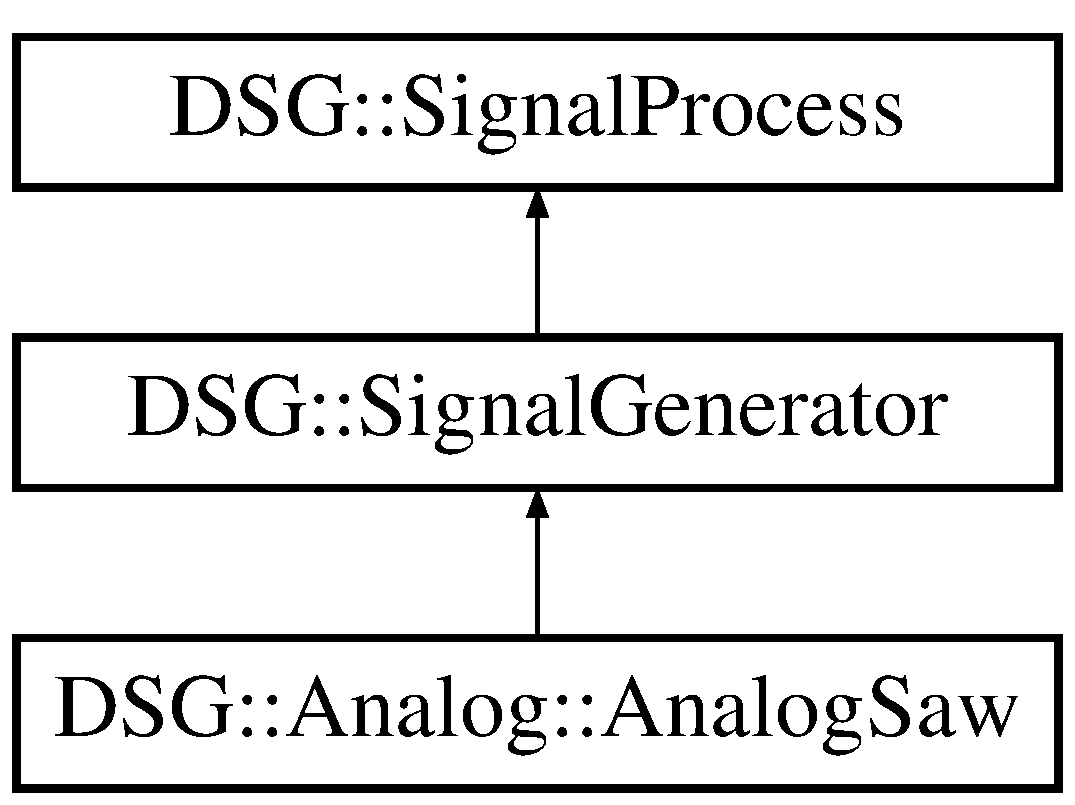
\includegraphics[height=3.000000cm]{class_d_s_g_1_1_analog_1_1_analog_saw}
\end{center}
\end{figure}
\subsection*{Public Member Functions}
\begin{DoxyCompactItemize}
\item 
\hyperlink{class_d_s_g_1_1_analog_1_1_analog_saw_abcb0b997be32413da0d14b93aeeb9c17}{Analog\+Saw} ()
\item 
\hyperlink{class_d_s_g_1_1_analog_1_1_analog_saw_ad110da0b337948fb70ecdfad7dbb5ddf}{Analog\+Saw} (\hyperlink{namespace_d_s_g_a4315a061386fa1014fda09b15d3a6973}{D\+S\+G\+::\+D\+S\+G\+Frequency} const \&frequency, \hyperlink{namespace_d_s_g_a44431ce1eb0a7300efdd207bc879e52c}{D\+S\+G\+::\+D\+S\+G\+Phase} const \&offset)
\item 
virtual \hyperlink{class_d_s_g_1_1_analog_1_1_analog_saw_a42a5fe22e0c3b9d1bd3996fe5bbd24ba}{$\sim$\+Analog\+Saw} ()
\item 
virtual bool \hyperlink{class_d_s_g_1_1_analog_1_1_analog_saw_a8d36e77c09ba84128e786c7bb14cddda}{Perform} (\hyperlink{namespace_d_s_g_ac39a94cd27ebcd9c1e7502d0c624894a}{D\+S\+G\+::\+D\+S\+G\+Sample} \&signal)
\item 
virtual bool \hyperlink{class_d_s_g_1_1_analog_1_1_analog_saw_a38f091059d924c9141fee3e27522e7e1}{Perform} (\hyperlink{class_d_s_g_1_1_ring_buffer}{D\+S\+G\+::\+Ring\+Buffer} \&signal)
\end{DoxyCompactItemize}
\subsection*{Protected Attributes}
\begin{DoxyCompactItemize}
\item 
\hyperlink{namespace_d_s_g_ac39a94cd27ebcd9c1e7502d0c624894a}{D\+S\+G\+::\+D\+S\+G\+Sample} \hyperlink{class_d_s_g_1_1_analog_1_1_analog_saw_a81a923800bb8ba0f788d3567d2965d2a}{\+\_\+stor}
\end{DoxyCompactItemize}
\subsection*{Additional Inherited Members}


\subsection{Detailed Description}
\hyperlink{class_d_s_g_1_1_analog_1_1_analog_saw}{D\+S\+G\+::\+Analog\+::\+Analog\+Saw} -\/ \hyperlink{namespace_d_s_g_1_1_analog}{Analog} Syle Saw Wave Generator. 

Definition at line \hyperlink{_analog_saw_8h_source_l00034}{34} of file \hyperlink{_analog_saw_8h_source}{Analog\+Saw.\+h}.



\subsection{Constructor \& Destructor Documentation}
\hypertarget{class_d_s_g_1_1_analog_1_1_analog_saw_abcb0b997be32413da0d14b93aeeb9c17}{\index{D\+S\+G\+::\+Analog\+::\+Analog\+Saw@{D\+S\+G\+::\+Analog\+::\+Analog\+Saw}!Analog\+Saw@{Analog\+Saw}}
\index{Analog\+Saw@{Analog\+Saw}!D\+S\+G\+::\+Analog\+::\+Analog\+Saw@{D\+S\+G\+::\+Analog\+::\+Analog\+Saw}}
\subsubsection[{Analog\+Saw}]{\setlength{\rightskip}{0pt plus 5cm}D\+S\+G\+::\+Analog\+::\+Analog\+Saw\+::\+Analog\+Saw (
\begin{DoxyParamCaption}
{}
\end{DoxyParamCaption}
)}}\label{class_d_s_g_1_1_analog_1_1_analog_saw_abcb0b997be32413da0d14b93aeeb9c17}


Definition at line \hyperlink{_analog_saw_8cpp_source_l00025}{25} of file \hyperlink{_analog_saw_8cpp_source}{Analog\+Saw.\+cpp}.


\begin{DoxyCode}
00025 :\hyperlink{class_d_s_g_1_1_signal_generator}{DSG::SignalGenerator}()\{\}
\end{DoxyCode}
\hypertarget{class_d_s_g_1_1_analog_1_1_analog_saw_ad110da0b337948fb70ecdfad7dbb5ddf}{\index{D\+S\+G\+::\+Analog\+::\+Analog\+Saw@{D\+S\+G\+::\+Analog\+::\+Analog\+Saw}!Analog\+Saw@{Analog\+Saw}}
\index{Analog\+Saw@{Analog\+Saw}!D\+S\+G\+::\+Analog\+::\+Analog\+Saw@{D\+S\+G\+::\+Analog\+::\+Analog\+Saw}}
\subsubsection[{Analog\+Saw}]{\setlength{\rightskip}{0pt plus 5cm}D\+S\+G\+::\+Analog\+::\+Analog\+Saw\+::\+Analog\+Saw (
\begin{DoxyParamCaption}
\item[{{\bf D\+S\+G\+::\+D\+S\+G\+Frequency} const \&}]{frequency, }
\item[{{\bf D\+S\+G\+::\+D\+S\+G\+Phase} const \&}]{offset}
\end{DoxyParamCaption}
)}}\label{class_d_s_g_1_1_analog_1_1_analog_saw_ad110da0b337948fb70ecdfad7dbb5ddf}


Definition at line \hyperlink{_analog_saw_8cpp_source_l00026}{26} of file \hyperlink{_analog_saw_8cpp_source}{Analog\+Saw.\+cpp}.


\begin{DoxyCode}
00026 :\hyperlink{class_d_s_g_1_1_signal_generator}{DSG::SignalGenerator}(frequency,offset)\{\}
\end{DoxyCode}
\hypertarget{class_d_s_g_1_1_analog_1_1_analog_saw_a42a5fe22e0c3b9d1bd3996fe5bbd24ba}{\index{D\+S\+G\+::\+Analog\+::\+Analog\+Saw@{D\+S\+G\+::\+Analog\+::\+Analog\+Saw}!````~Analog\+Saw@{$\sim$\+Analog\+Saw}}
\index{````~Analog\+Saw@{$\sim$\+Analog\+Saw}!D\+S\+G\+::\+Analog\+::\+Analog\+Saw@{D\+S\+G\+::\+Analog\+::\+Analog\+Saw}}
\subsubsection[{$\sim$\+Analog\+Saw}]{\setlength{\rightskip}{0pt plus 5cm}D\+S\+G\+::\+Analog\+::\+Analog\+Saw\+::$\sim$\+Analog\+Saw (
\begin{DoxyParamCaption}
{}
\end{DoxyParamCaption}
)\hspace{0.3cm}{\ttfamily [virtual]}}}\label{class_d_s_g_1_1_analog_1_1_analog_saw_a42a5fe22e0c3b9d1bd3996fe5bbd24ba}


Definition at line \hyperlink{_analog_saw_8cpp_source_l00027}{27} of file \hyperlink{_analog_saw_8cpp_source}{Analog\+Saw.\+cpp}.


\begin{DoxyCode}
00027 \{\}\end{DoxyCode}


\subsection{Member Function Documentation}
\hypertarget{class_d_s_g_1_1_analog_1_1_analog_saw_a8d36e77c09ba84128e786c7bb14cddda}{\index{D\+S\+G\+::\+Analog\+::\+Analog\+Saw@{D\+S\+G\+::\+Analog\+::\+Analog\+Saw}!Perform@{Perform}}
\index{Perform@{Perform}!D\+S\+G\+::\+Analog\+::\+Analog\+Saw@{D\+S\+G\+::\+Analog\+::\+Analog\+Saw}}
\subsubsection[{Perform}]{\setlength{\rightskip}{0pt plus 5cm}bool D\+S\+G\+::\+Analog\+::\+Analog\+Saw\+::\+Perform (
\begin{DoxyParamCaption}
\item[{{\bf D\+S\+G\+::\+D\+S\+G\+Sample} \&}]{signal}
\end{DoxyParamCaption}
)\hspace{0.3cm}{\ttfamily [inline]}, {\ttfamily [virtual]}}}\label{class_d_s_g_1_1_analog_1_1_analog_saw_a8d36e77c09ba84128e786c7bb14cddda}


Reimplemented from \hyperlink{class_d_s_g_1_1_signal_generator_a46fe75a81a242e191c5049d33ddf4155}{D\+S\+G\+::\+Signal\+Generator}.



Definition at line \hyperlink{_analog_saw_8h_source_l00044}{44} of file \hyperlink{_analog_saw_8h_source}{Analog\+Saw.\+h}.


\begin{DoxyCode}
00044                                                                    \{
00045             \hyperlink{class_d_s_g_1_1_analog_1_1_analog_saw_a81a923800bb8ba0f788d3567d2965d2a}{\_stor}=\hyperlink{class_d_s_g_1_1_phasor_a82c148d71128cfc518fc8e7e131c3a38}{\_phasor};
00046             \hyperlink{class_d_s_g_1_1_analog_1_1_analog_saw_a81a923800bb8ba0f788d3567d2965d2a}{\_stor}+=0.5;
00047             \textcolor{keywordflow}{if} (\hyperlink{class_d_s_g_1_1_analog_1_1_analog_saw_a81a923800bb8ba0f788d3567d2965d2a}{\_stor}>1.0) \{
00048                 --\hyperlink{class_d_s_g_1_1_analog_1_1_analog_saw_a81a923800bb8ba0f788d3567d2965d2a}{\_stor};
00049             \}
00050             \hyperlink{class_d_s_g_1_1_analog_1_1_analog_saw_a81a923800bb8ba0f788d3567d2965d2a}{\_stor}-=0.5;
00051             \hyperlink{class_d_s_g_1_1_analog_1_1_analog_saw_a81a923800bb8ba0f788d3567d2965d2a}{\_stor}*=2.0;
00052             signal=\hyperlink{class_d_s_g_1_1_analog_1_1_analog_saw_a81a923800bb8ba0f788d3567d2965d2a}{\_stor};
00053             \hyperlink{class_d_s_g_1_1_phasor_a6a088b29e506fb5e99d73f4f0160c583}{step}();
00054             \textcolor{keywordflow}{return} \textcolor{keyword}{true};
00055         \}
\end{DoxyCode}
\hypertarget{class_d_s_g_1_1_analog_1_1_analog_saw_a38f091059d924c9141fee3e27522e7e1}{\index{D\+S\+G\+::\+Analog\+::\+Analog\+Saw@{D\+S\+G\+::\+Analog\+::\+Analog\+Saw}!Perform@{Perform}}
\index{Perform@{Perform}!D\+S\+G\+::\+Analog\+::\+Analog\+Saw@{D\+S\+G\+::\+Analog\+::\+Analog\+Saw}}
\subsubsection[{Perform}]{\setlength{\rightskip}{0pt plus 5cm}bool D\+S\+G\+::\+Analog\+::\+Analog\+Saw\+::\+Perform (
\begin{DoxyParamCaption}
\item[{{\bf D\+S\+G\+::\+Ring\+Buffer} \&}]{signal}
\end{DoxyParamCaption}
)\hspace{0.3cm}{\ttfamily [inline]}, {\ttfamily [virtual]}}}\label{class_d_s_g_1_1_analog_1_1_analog_saw_a38f091059d924c9141fee3e27522e7e1}


Reimplemented from \hyperlink{class_d_s_g_1_1_signal_generator_ab050f80e84e6c8b3e354b56930d6a02b}{D\+S\+G\+::\+Signal\+Generator}.



Definition at line \hyperlink{_analog_saw_8h_source_l00056}{56} of file \hyperlink{_analog_saw_8h_source}{Analog\+Saw.\+h}.


\begin{DoxyCode}
00056                                                                     \{
00057             signal.\hyperlink{class_d_s_g_1_1_ring_buffer_ab23c8003d2857809a816068eeb209d60}{Flush}();
00058             \textcolor{keywordflow}{while} (!signal.\hyperlink{class_d_s_g_1_1_ring_buffer_a53ddb04ffcbb5470a8d2b0a3c65b70cb}{Full}()) \{
00059                 \textcolor{keywordflow}{if} (\hyperlink{class_d_s_g_1_1_analog_1_1_analog_saw_a8d36e77c09ba84128e786c7bb14cddda}{Perform}(\hyperlink{class_d_s_g_1_1_signal_generator_a28a9b47a1aa0783029f11a19ba0363f2}{\_storage})) \{
00060                     \textcolor{keywordflow}{if}(signal.\hyperlink{class_d_s_g_1_1_ring_buffer_aa5dd2caa0a270173251faee40a43d692}{Write}(\hyperlink{class_d_s_g_1_1_signal_generator_a28a9b47a1aa0783029f11a19ba0363f2}{\_storage}))\{
00061                     \}\textcolor{keywordflow}{else} \textcolor{keywordflow}{return} \textcolor{keyword}{false};
00062                 \}\textcolor{keywordflow}{else} \textcolor{keywordflow}{return} \textcolor{keyword}{false};
00063             \}\textcolor{keywordflow}{return} \textcolor{keyword}{true};
00064         \}
\end{DoxyCode}


\subsection{Member Data Documentation}
\hypertarget{class_d_s_g_1_1_analog_1_1_analog_saw_a81a923800bb8ba0f788d3567d2965d2a}{\index{D\+S\+G\+::\+Analog\+::\+Analog\+Saw@{D\+S\+G\+::\+Analog\+::\+Analog\+Saw}!\+\_\+stor@{\+\_\+stor}}
\index{\+\_\+stor@{\+\_\+stor}!D\+S\+G\+::\+Analog\+::\+Analog\+Saw@{D\+S\+G\+::\+Analog\+::\+Analog\+Saw}}
\subsubsection[{\+\_\+stor}]{\setlength{\rightskip}{0pt plus 5cm}{\bf D\+S\+G\+::\+D\+S\+G\+Sample} D\+S\+G\+::\+Analog\+::\+Analog\+Saw\+::\+\_\+stor\hspace{0.3cm}{\ttfamily [protected]}}}\label{class_d_s_g_1_1_analog_1_1_analog_saw_a81a923800bb8ba0f788d3567d2965d2a}


Definition at line \hyperlink{_analog_saw_8h_source_l00042}{42} of file \hyperlink{_analog_saw_8h_source}{Analog\+Saw.\+h}.



The documentation for this class was generated from the following files\+:\begin{DoxyCompactItemize}
\item 
\hyperlink{_analog_saw_8h}{Analog\+Saw.\+h}\item 
\hyperlink{_analog_saw_8cpp}{Analog\+Saw.\+cpp}\end{DoxyCompactItemize}

\hypertarget{class_d_s_g_1_1_analog_1_1_analog_square}{\section{D\+S\+G\+:\+:Analog\+:\+:Analog\+Square Class Reference}
\label{class_d_s_g_1_1_analog_1_1_analog_square}\index{D\+S\+G\+::\+Analog\+::\+Analog\+Square@{D\+S\+G\+::\+Analog\+::\+Analog\+Square}}
}


D\+S\+G\+::\+Analog\+Square -\/ \hyperlink{namespace_d_s_g_1_1_analog}{Analog} Syle Square Wave Generator.  




{\ttfamily \#include $<$Analog\+Square.\+h$>$}

Inheritance diagram for D\+S\+G\+:\+:Analog\+:\+:Analog\+Square\+:\begin{figure}[H]
\begin{center}
\leavevmode
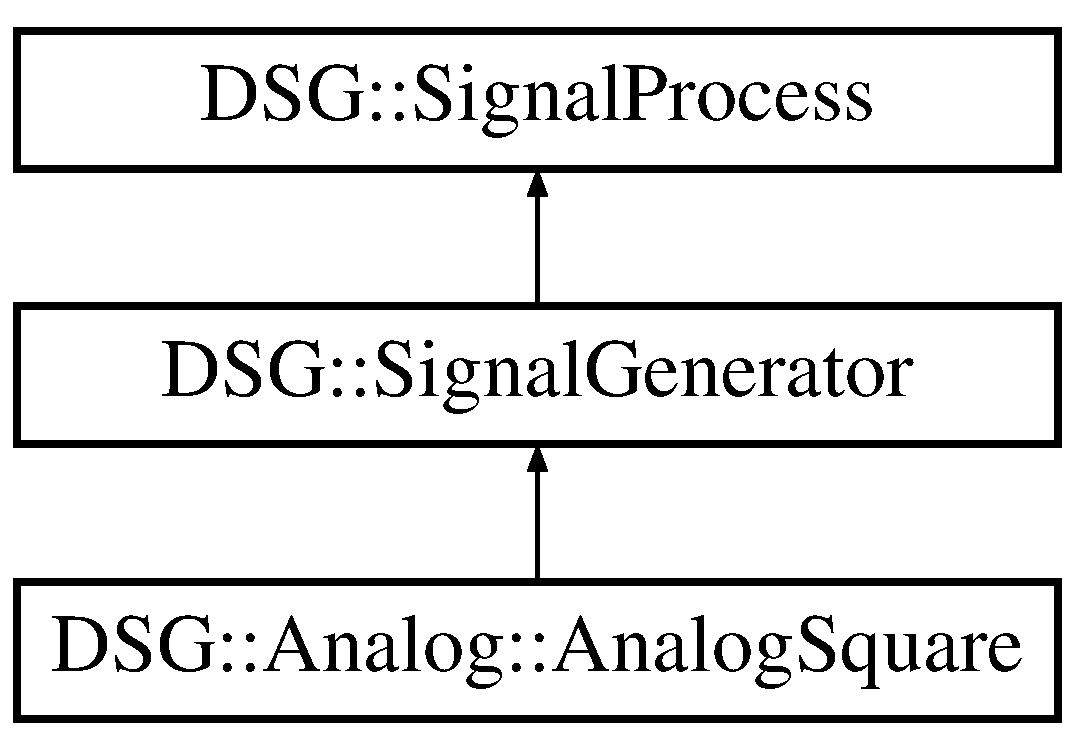
\includegraphics[height=3.000000cm]{class_d_s_g_1_1_analog_1_1_analog_square}
\end{center}
\end{figure}
\subsection*{Public Member Functions}
\begin{DoxyCompactItemize}
\item 
\hypertarget{class_d_s_g_1_1_analog_1_1_analog_square_a886eb67edded43efca895741559a55f4}{{\bfseries Analog\+Square} (D\+S\+G\+::\+D\+S\+G\+Frequency const \&frequency, D\+S\+G\+::\+D\+S\+G\+Phase const \&offset)}\label{class_d_s_g_1_1_analog_1_1_analog_square_a886eb67edded43efca895741559a55f4}

\item 
\hypertarget{class_d_s_g_1_1_analog_1_1_analog_square_a784aa17d266704647789b972cf880e9f}{virtual bool {\bfseries Perform} (D\+S\+G\+::\+D\+S\+G\+Sample \&signal)}\label{class_d_s_g_1_1_analog_1_1_analog_square_a784aa17d266704647789b972cf880e9f}

\item 
\hypertarget{class_d_s_g_1_1_analog_1_1_analog_square_af4d41d5894ae02e920c61e06cf041c60}{virtual bool {\bfseries Perform} (\hyperlink{class_d_s_g_1_1_ring_buffer}{D\+S\+G\+::\+Ring\+Buffer} \&signal)}\label{class_d_s_g_1_1_analog_1_1_analog_square_af4d41d5894ae02e920c61e06cf041c60}

\end{DoxyCompactItemize}
\subsection*{Additional Inherited Members}


\subsection{Detailed Description}
D\+S\+G\+::\+Analog\+Square -\/ \hyperlink{namespace_d_s_g_1_1_analog}{Analog} Syle Square Wave Generator. 

The documentation for this class was generated from the following files\+:\begin{DoxyCompactItemize}
\item 
/\+Users/alexanderzywicki/\+Documents/\+D\+S\+G/src/Analog\+Square.\+h\item 
/\+Users/alexanderzywicki/\+Documents/\+D\+S\+G/src/Analog\+Square.\+cpp\end{DoxyCompactItemize}

\hypertarget{class_d_s_g_1_1_analog_1_1_analog_triangle}{\section{D\+S\+G\+:\+:Analog\+:\+:Analog\+Triangle Class Reference}
\label{class_d_s_g_1_1_analog_1_1_analog_triangle}\index{D\+S\+G\+::\+Analog\+::\+Analog\+Triangle@{D\+S\+G\+::\+Analog\+::\+Analog\+Triangle}}
}


\hyperlink{class_d_s_g_1_1_analog_1_1_analog_triangle}{D\+S\+G\+::\+Analog\+::\+Analog\+Triangle} -\/ \hyperlink{namespace_d_s_g_1_1_analog}{Analog} Syle Triangle Wave Generator.  




{\ttfamily \#include $<$Analog\+Triangle.\+h$>$}

Inheritance diagram for D\+S\+G\+:\+:Analog\+:\+:Analog\+Triangle\+:\begin{figure}[H]
\begin{center}
\leavevmode
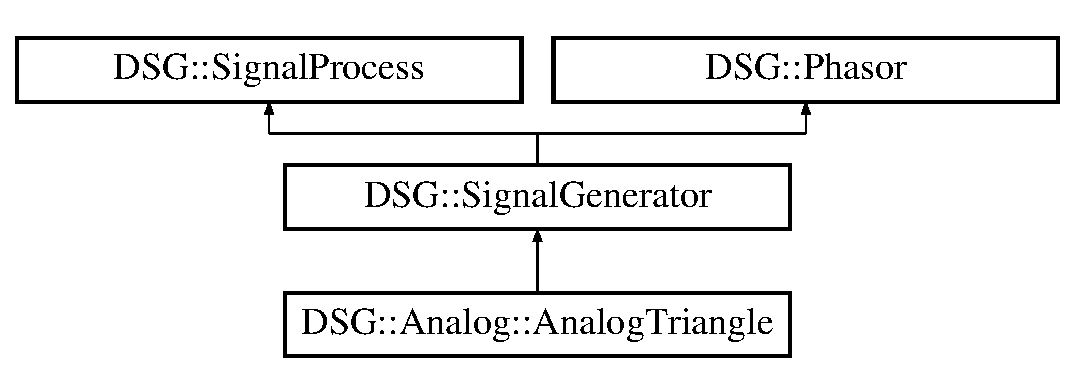
\includegraphics[height=3.000000cm]{class_d_s_g_1_1_analog_1_1_analog_triangle}
\end{center}
\end{figure}
\subsection*{Public Member Functions}
\begin{DoxyCompactItemize}
\item 
\hyperlink{class_d_s_g_1_1_analog_1_1_analog_triangle_a2fe1a7a29eb9472323a2a1c0d0696e55}{Analog\+Triangle} ()
\item 
\hyperlink{class_d_s_g_1_1_analog_1_1_analog_triangle_a75c0a8b20e1843b35de3944da11c75ed}{Analog\+Triangle} (\hyperlink{namespace_d_s_g_a4315a061386fa1014fda09b15d3a6973}{D\+S\+G\+::\+D\+S\+G\+Frequency} const \&frequency, \hyperlink{namespace_d_s_g_a44431ce1eb0a7300efdd207bc879e52c}{D\+S\+G\+::\+D\+S\+G\+Phase} const \&offset)
\item 
virtual \hyperlink{class_d_s_g_1_1_analog_1_1_analog_triangle_af6e127d2fb623afad9b172e7c8b3c656}{$\sim$\+Analog\+Triangle} ()
\item 
virtual bool \hyperlink{class_d_s_g_1_1_analog_1_1_analog_triangle_a9b2484f3eb4c4ad545cb88b8833be124}{Perform} (\hyperlink{namespace_d_s_g_ac39a94cd27ebcd9c1e7502d0c624894a}{D\+S\+G\+::\+D\+S\+G\+Sample} \&signal)
\item 
virtual bool \hyperlink{class_d_s_g_1_1_analog_1_1_analog_triangle_a568c994e0f83f6a01d813357259a8f37}{Perform} (\hyperlink{class_d_s_g_1_1_ring_buffer}{D\+S\+G\+::\+Ring\+Buffer} \&signal)
\end{DoxyCompactItemize}
\subsection*{Protected Attributes}
\begin{DoxyCompactItemize}
\item 
\hyperlink{namespace_d_s_g_ac39a94cd27ebcd9c1e7502d0c624894a}{D\+S\+G\+::\+D\+S\+G\+Sample} \hyperlink{class_d_s_g_1_1_analog_1_1_analog_triangle_ac93bccb7e366491f45ea9c3af04072ae}{\+\_\+stor}
\end{DoxyCompactItemize}
\subsection*{Additional Inherited Members}


\subsection{Detailed Description}
\hyperlink{class_d_s_g_1_1_analog_1_1_analog_triangle}{D\+S\+G\+::\+Analog\+::\+Analog\+Triangle} -\/ \hyperlink{namespace_d_s_g_1_1_analog}{Analog} Syle Triangle Wave Generator. 

Definition at line \hyperlink{_analog_triangle_8h_source_l00034}{34} of file \hyperlink{_analog_triangle_8h_source}{Analog\+Triangle.\+h}.



\subsection{Constructor \& Destructor Documentation}
\hypertarget{class_d_s_g_1_1_analog_1_1_analog_triangle_a2fe1a7a29eb9472323a2a1c0d0696e55}{\index{D\+S\+G\+::\+Analog\+::\+Analog\+Triangle@{D\+S\+G\+::\+Analog\+::\+Analog\+Triangle}!Analog\+Triangle@{Analog\+Triangle}}
\index{Analog\+Triangle@{Analog\+Triangle}!D\+S\+G\+::\+Analog\+::\+Analog\+Triangle@{D\+S\+G\+::\+Analog\+::\+Analog\+Triangle}}
\subsubsection[{Analog\+Triangle}]{\setlength{\rightskip}{0pt plus 5cm}D\+S\+G\+::\+Analog\+::\+Analog\+Triangle\+::\+Analog\+Triangle (
\begin{DoxyParamCaption}
{}
\end{DoxyParamCaption}
)}}\label{class_d_s_g_1_1_analog_1_1_analog_triangle_a2fe1a7a29eb9472323a2a1c0d0696e55}


Definition at line \hyperlink{_analog_triangle_8cpp_source_l00025}{25} of file \hyperlink{_analog_triangle_8cpp_source}{Analog\+Triangle.\+cpp}.


\begin{DoxyCode}
00025 :\hyperlink{class_d_s_g_1_1_signal_generator}{DSG::SignalGenerator}()\{\}
\end{DoxyCode}
\hypertarget{class_d_s_g_1_1_analog_1_1_analog_triangle_a75c0a8b20e1843b35de3944da11c75ed}{\index{D\+S\+G\+::\+Analog\+::\+Analog\+Triangle@{D\+S\+G\+::\+Analog\+::\+Analog\+Triangle}!Analog\+Triangle@{Analog\+Triangle}}
\index{Analog\+Triangle@{Analog\+Triangle}!D\+S\+G\+::\+Analog\+::\+Analog\+Triangle@{D\+S\+G\+::\+Analog\+::\+Analog\+Triangle}}
\subsubsection[{Analog\+Triangle}]{\setlength{\rightskip}{0pt plus 5cm}D\+S\+G\+::\+Analog\+::\+Analog\+Triangle\+::\+Analog\+Triangle (
\begin{DoxyParamCaption}
\item[{{\bf D\+S\+G\+::\+D\+S\+G\+Frequency} const \&}]{frequency, }
\item[{{\bf D\+S\+G\+::\+D\+S\+G\+Phase} const \&}]{offset}
\end{DoxyParamCaption}
)}}\label{class_d_s_g_1_1_analog_1_1_analog_triangle_a75c0a8b20e1843b35de3944da11c75ed}


Definition at line \hyperlink{_analog_triangle_8cpp_source_l00026}{26} of file \hyperlink{_analog_triangle_8cpp_source}{Analog\+Triangle.\+cpp}.


\begin{DoxyCode}
00026 :\hyperlink{class_d_s_g_1_1_signal_generator}{DSG::SignalGenerator}(frequency,offset)\{\}
\end{DoxyCode}
\hypertarget{class_d_s_g_1_1_analog_1_1_analog_triangle_af6e127d2fb623afad9b172e7c8b3c656}{\index{D\+S\+G\+::\+Analog\+::\+Analog\+Triangle@{D\+S\+G\+::\+Analog\+::\+Analog\+Triangle}!````~Analog\+Triangle@{$\sim$\+Analog\+Triangle}}
\index{````~Analog\+Triangle@{$\sim$\+Analog\+Triangle}!D\+S\+G\+::\+Analog\+::\+Analog\+Triangle@{D\+S\+G\+::\+Analog\+::\+Analog\+Triangle}}
\subsubsection[{$\sim$\+Analog\+Triangle}]{\setlength{\rightskip}{0pt plus 5cm}D\+S\+G\+::\+Analog\+::\+Analog\+Triangle\+::$\sim$\+Analog\+Triangle (
\begin{DoxyParamCaption}
{}
\end{DoxyParamCaption}
)\hspace{0.3cm}{\ttfamily [virtual]}}}\label{class_d_s_g_1_1_analog_1_1_analog_triangle_af6e127d2fb623afad9b172e7c8b3c656}


Definition at line \hyperlink{_analog_triangle_8cpp_source_l00027}{27} of file \hyperlink{_analog_triangle_8cpp_source}{Analog\+Triangle.\+cpp}.


\begin{DoxyCode}
00027 \{\}\end{DoxyCode}


\subsection{Member Function Documentation}
\hypertarget{class_d_s_g_1_1_analog_1_1_analog_triangle_a9b2484f3eb4c4ad545cb88b8833be124}{\index{D\+S\+G\+::\+Analog\+::\+Analog\+Triangle@{D\+S\+G\+::\+Analog\+::\+Analog\+Triangle}!Perform@{Perform}}
\index{Perform@{Perform}!D\+S\+G\+::\+Analog\+::\+Analog\+Triangle@{D\+S\+G\+::\+Analog\+::\+Analog\+Triangle}}
\subsubsection[{Perform}]{\setlength{\rightskip}{0pt plus 5cm}bool D\+S\+G\+::\+Analog\+::\+Analog\+Triangle\+::\+Perform (
\begin{DoxyParamCaption}
\item[{{\bf D\+S\+G\+::\+D\+S\+G\+Sample} \&}]{signal}
\end{DoxyParamCaption}
)\hspace{0.3cm}{\ttfamily [inline]}, {\ttfamily [virtual]}}}\label{class_d_s_g_1_1_analog_1_1_analog_triangle_a9b2484f3eb4c4ad545cb88b8833be124}


Reimplemented from \hyperlink{class_d_s_g_1_1_signal_generator_a46fe75a81a242e191c5049d33ddf4155}{D\+S\+G\+::\+Signal\+Generator}.



Definition at line \hyperlink{_analog_triangle_8h_source_l00044}{44} of file \hyperlink{_analog_triangle_8h_source}{Analog\+Triangle.\+h}.


\begin{DoxyCode}
00044                                                                         \{
00045             \hyperlink{class_d_s_g_1_1_analog_1_1_analog_triangle_ac93bccb7e366491f45ea9c3af04072ae}{\_stor} = \hyperlink{class_d_s_g_1_1_phasor_a82c148d71128cfc518fc8e7e131c3a38}{\_phasor};
00046             \hyperlink{class_d_s_g_1_1_analog_1_1_analog_triangle_ac93bccb7e366491f45ea9c3af04072ae}{\_stor}+=0.25;
00047             \textcolor{keywordflow}{while} (\hyperlink{class_d_s_g_1_1_analog_1_1_analog_triangle_ac93bccb7e366491f45ea9c3af04072ae}{\_stor}>1.0) \{
00048                 \hyperlink{class_d_s_g_1_1_analog_1_1_analog_triangle_ac93bccb7e366491f45ea9c3af04072ae}{\_stor}-=1.0;
00049             \}
00050             \hyperlink{class_d_s_g_1_1_analog_1_1_analog_triangle_ac93bccb7e366491f45ea9c3af04072ae}{\_stor}-=0.5;
00051             \textcolor{keywordflow}{if} (\hyperlink{class_d_s_g_1_1_analog_1_1_analog_triangle_ac93bccb7e366491f45ea9c3af04072ae}{\_stor}<0) \{
00052                 \hyperlink{class_d_s_g_1_1_analog_1_1_analog_triangle_ac93bccb7e366491f45ea9c3af04072ae}{\_stor}*=-1.0;
00053             \}
00054             \hyperlink{class_d_s_g_1_1_analog_1_1_analog_triangle_ac93bccb7e366491f45ea9c3af04072ae}{\_stor}-=0.25;
00055             \hyperlink{class_d_s_g_1_1_analog_1_1_analog_triangle_ac93bccb7e366491f45ea9c3af04072ae}{\_stor}*=-4.0;
00056             signal = \hyperlink{class_d_s_g_1_1_analog_1_1_analog_triangle_ac93bccb7e366491f45ea9c3af04072ae}{\_stor};
00057             \hyperlink{class_d_s_g_1_1_phasor_a6a088b29e506fb5e99d73f4f0160c583}{step}();\textcolor{comment}{//always last}
00058             \textcolor{keywordflow}{return} \textcolor{keyword}{true};
00059         \}
\end{DoxyCode}
\hypertarget{class_d_s_g_1_1_analog_1_1_analog_triangle_a568c994e0f83f6a01d813357259a8f37}{\index{D\+S\+G\+::\+Analog\+::\+Analog\+Triangle@{D\+S\+G\+::\+Analog\+::\+Analog\+Triangle}!Perform@{Perform}}
\index{Perform@{Perform}!D\+S\+G\+::\+Analog\+::\+Analog\+Triangle@{D\+S\+G\+::\+Analog\+::\+Analog\+Triangle}}
\subsubsection[{Perform}]{\setlength{\rightskip}{0pt plus 5cm}bool D\+S\+G\+::\+Analog\+::\+Analog\+Triangle\+::\+Perform (
\begin{DoxyParamCaption}
\item[{{\bf D\+S\+G\+::\+Ring\+Buffer} \&}]{signal}
\end{DoxyParamCaption}
)\hspace{0.3cm}{\ttfamily [inline]}, {\ttfamily [virtual]}}}\label{class_d_s_g_1_1_analog_1_1_analog_triangle_a568c994e0f83f6a01d813357259a8f37}


Reimplemented from \hyperlink{class_d_s_g_1_1_signal_generator_ab050f80e84e6c8b3e354b56930d6a02b}{D\+S\+G\+::\+Signal\+Generator}.



Definition at line \hyperlink{_analog_triangle_8h_source_l00060}{60} of file \hyperlink{_analog_triangle_8h_source}{Analog\+Triangle.\+h}.


\begin{DoxyCode}
00060                                                                          \{
00061             signal.\hyperlink{class_d_s_g_1_1_ring_buffer_ab23c8003d2857809a816068eeb209d60}{Flush}();
00062             \textcolor{keywordflow}{while} (!signal.\hyperlink{class_d_s_g_1_1_ring_buffer_a53ddb04ffcbb5470a8d2b0a3c65b70cb}{Full}()) \{
00063                 \textcolor{keywordflow}{if} (\hyperlink{class_d_s_g_1_1_analog_1_1_analog_triangle_a9b2484f3eb4c4ad545cb88b8833be124}{Perform}(\hyperlink{class_d_s_g_1_1_signal_generator_a28a9b47a1aa0783029f11a19ba0363f2}{\_storage})) \{
00064                     \textcolor{keywordflow}{if}(signal.\hyperlink{class_d_s_g_1_1_ring_buffer_aa5dd2caa0a270173251faee40a43d692}{Write}(\hyperlink{class_d_s_g_1_1_signal_generator_a28a9b47a1aa0783029f11a19ba0363f2}{\_storage}))\{
00065                     \}\textcolor{keywordflow}{else} \textcolor{keywordflow}{return} \textcolor{keyword}{false};
00066                 \}\textcolor{keywordflow}{else} \textcolor{keywordflow}{return} \textcolor{keyword}{false};
00067             \}\textcolor{keywordflow}{return} \textcolor{keyword}{true};
00068         \}
\end{DoxyCode}


\subsection{Member Data Documentation}
\hypertarget{class_d_s_g_1_1_analog_1_1_analog_triangle_ac93bccb7e366491f45ea9c3af04072ae}{\index{D\+S\+G\+::\+Analog\+::\+Analog\+Triangle@{D\+S\+G\+::\+Analog\+::\+Analog\+Triangle}!\+\_\+stor@{\+\_\+stor}}
\index{\+\_\+stor@{\+\_\+stor}!D\+S\+G\+::\+Analog\+::\+Analog\+Triangle@{D\+S\+G\+::\+Analog\+::\+Analog\+Triangle}}
\subsubsection[{\+\_\+stor}]{\setlength{\rightskip}{0pt plus 5cm}{\bf D\+S\+G\+::\+D\+S\+G\+Sample} D\+S\+G\+::\+Analog\+::\+Analog\+Triangle\+::\+\_\+stor\hspace{0.3cm}{\ttfamily [protected]}}}\label{class_d_s_g_1_1_analog_1_1_analog_triangle_ac93bccb7e366491f45ea9c3af04072ae}


Definition at line \hyperlink{_analog_triangle_8h_source_l00042}{42} of file \hyperlink{_analog_triangle_8h_source}{Analog\+Triangle.\+h}.



The documentation for this class was generated from the following files\+:\begin{DoxyCompactItemize}
\item 
\hyperlink{_analog_triangle_8h}{Analog\+Triangle.\+h}\item 
\hyperlink{_analog_triangle_8cpp}{Analog\+Triangle.\+cpp}\end{DoxyCompactItemize}

\hypertarget{class_d_s_g_1_1_audio_settings}{\section{D\+S\+G\+:\+:Audio\+Settings Class Reference}
\label{class_d_s_g_1_1_audio_settings}\index{D\+S\+G\+::\+Audio\+Settings@{D\+S\+G\+::\+Audio\+Settings}}
}


\hyperlink{class_d_s_g_1_1_audio_settings}{D\+S\+G\+::\+Audio\+Settings} -\/ Global Storage For Audio Settings Such As Sample Rate.  




{\ttfamily \#include $<$Audio\+Settings.\+h$>$}

\subsection*{Static Public Member Functions}
\begin{DoxyCompactItemize}
\item 
static \hyperlink{namespace_d_s_g_a4315a061386fa1014fda09b15d3a6973}{D\+S\+G\+::\+D\+S\+G\+Frequency} const \& \hyperlink{class_d_s_g_1_1_audio_settings_a4f459c389b10c11828e2f2f00c012c49}{Sample\+Rate} ()
\item 
static \hyperlink{namespace_d_s_g_a4315a061386fa1014fda09b15d3a6973}{D\+S\+G\+::\+D\+S\+G\+Frequency} const \& \hyperlink{class_d_s_g_1_1_audio_settings_a9c5640e47b6eaa4331a0e5053abb1314}{Sample\+Rate} (\hyperlink{namespace_d_s_g_a4315a061386fa1014fda09b15d3a6973}{D\+S\+G\+::\+D\+S\+G\+Frequency} const \&value)
\item 
static \hyperlink{namespace_d_s_g_a4315a061386fa1014fda09b15d3a6973}{D\+S\+G\+::\+D\+S\+G\+Frequency} const \& \hyperlink{class_d_s_g_1_1_audio_settings_a8cb4afd7b58e927300ff46fbeb71bec7}{Nyquist} ()
\end{DoxyCompactItemize}
\subsection*{Static Protected Attributes}
\begin{DoxyCompactItemize}
\item 
static \hyperlink{namespace_d_s_g_a4315a061386fa1014fda09b15d3a6973}{D\+S\+G\+::\+D\+S\+G\+Frequency} \hyperlink{class_d_s_g_1_1_audio_settings_a56869b51933f102b197f54001c8a1d27}{\+\_\+sample\+Rate}
\item 
static \hyperlink{namespace_d_s_g_a4315a061386fa1014fda09b15d3a6973}{D\+S\+G\+::\+D\+S\+G\+Frequency} \hyperlink{class_d_s_g_1_1_audio_settings_af3c7cbd15390d9bcbe39983c069390b5}{\+\_\+nyquist}
\end{DoxyCompactItemize}


\subsection{Detailed Description}
\hyperlink{class_d_s_g_1_1_audio_settings}{D\+S\+G\+::\+Audio\+Settings} -\/ Global Storage For Audio Settings Such As Sample Rate. 

Definition at line \hyperlink{_audio_settings_8h_source_l00014}{14} of file \hyperlink{_audio_settings_8h_source}{Audio\+Settings.\+h}.



\subsection{Member Function Documentation}
\hypertarget{class_d_s_g_1_1_audio_settings_a8cb4afd7b58e927300ff46fbeb71bec7}{\index{D\+S\+G\+::\+Audio\+Settings@{D\+S\+G\+::\+Audio\+Settings}!Nyquist@{Nyquist}}
\index{Nyquist@{Nyquist}!D\+S\+G\+::\+Audio\+Settings@{D\+S\+G\+::\+Audio\+Settings}}
\subsubsection[{Nyquist}]{\setlength{\rightskip}{0pt plus 5cm}{\bf D\+S\+G\+::\+D\+S\+G\+Frequency} const \& D\+S\+G\+::\+Audio\+Settings\+::\+Nyquist (
\begin{DoxyParamCaption}
{}
\end{DoxyParamCaption}
)\hspace{0.3cm}{\ttfamily [static]}}}\label{class_d_s_g_1_1_audio_settings_a8cb4afd7b58e927300ff46fbeb71bec7}


Definition at line \hyperlink{_audio_settings_8cpp_source_l00019}{19} of file \hyperlink{_audio_settings_8cpp_source}{Audio\+Settings.\+cpp}.


\begin{DoxyCode}
00019                                                 \{
00020     \textcolor{keywordflow}{return} \hyperlink{class_d_s_g_1_1_audio_settings_af3c7cbd15390d9bcbe39983c069390b5}{\_nyquist};
00021 \}\end{DoxyCode}
\hypertarget{class_d_s_g_1_1_audio_settings_a4f459c389b10c11828e2f2f00c012c49}{\index{D\+S\+G\+::\+Audio\+Settings@{D\+S\+G\+::\+Audio\+Settings}!Sample\+Rate@{Sample\+Rate}}
\index{Sample\+Rate@{Sample\+Rate}!D\+S\+G\+::\+Audio\+Settings@{D\+S\+G\+::\+Audio\+Settings}}
\subsubsection[{Sample\+Rate}]{\setlength{\rightskip}{0pt plus 5cm}{\bf D\+S\+G\+::\+D\+S\+G\+Frequency} const \& D\+S\+G\+::\+Audio\+Settings\+::\+Sample\+Rate (
\begin{DoxyParamCaption}
{}
\end{DoxyParamCaption}
)\hspace{0.3cm}{\ttfamily [static]}}}\label{class_d_s_g_1_1_audio_settings_a4f459c389b10c11828e2f2f00c012c49}


Definition at line \hyperlink{_audio_settings_8cpp_source_l00011}{11} of file \hyperlink{_audio_settings_8cpp_source}{Audio\+Settings.\+cpp}.


\begin{DoxyCode}
00011                                                    \{
00012     \textcolor{keywordflow}{return} \hyperlink{class_d_s_g_1_1_audio_settings_a56869b51933f102b197f54001c8a1d27}{\_sampleRate};
00013 \}
\end{DoxyCode}
\hypertarget{class_d_s_g_1_1_audio_settings_a9c5640e47b6eaa4331a0e5053abb1314}{\index{D\+S\+G\+::\+Audio\+Settings@{D\+S\+G\+::\+Audio\+Settings}!Sample\+Rate@{Sample\+Rate}}
\index{Sample\+Rate@{Sample\+Rate}!D\+S\+G\+::\+Audio\+Settings@{D\+S\+G\+::\+Audio\+Settings}}
\subsubsection[{Sample\+Rate}]{\setlength{\rightskip}{0pt plus 5cm}{\bf D\+S\+G\+::\+D\+S\+G\+Frequency} const \& D\+S\+G\+::\+Audio\+Settings\+::\+Sample\+Rate (
\begin{DoxyParamCaption}
\item[{{\bf D\+S\+G\+::\+D\+S\+G\+Frequency} const \&}]{value}
\end{DoxyParamCaption}
)\hspace{0.3cm}{\ttfamily [static]}}}\label{class_d_s_g_1_1_audio_settings_a9c5640e47b6eaa4331a0e5053abb1314}


Definition at line \hyperlink{_audio_settings_8cpp_source_l00014}{14} of file \hyperlink{_audio_settings_8cpp_source}{Audio\+Settings.\+cpp}.


\begin{DoxyCode}
00014                                                                                \{
00015     \hyperlink{class_d_s_g_1_1_audio_settings_a56869b51933f102b197f54001c8a1d27}{\_sampleRate} = value;
00016     \hyperlink{class_d_s_g_1_1_audio_settings_af3c7cbd15390d9bcbe39983c069390b5}{\_nyquist} = \hyperlink{class_d_s_g_1_1_audio_settings_a56869b51933f102b197f54001c8a1d27}{\_sampleRate}*0.5;
00017     \textcolor{keywordflow}{return} \hyperlink{class_d_s_g_1_1_audio_settings_a56869b51933f102b197f54001c8a1d27}{\_sampleRate};
00018 \}
\end{DoxyCode}


\subsection{Member Data Documentation}
\hypertarget{class_d_s_g_1_1_audio_settings_af3c7cbd15390d9bcbe39983c069390b5}{\index{D\+S\+G\+::\+Audio\+Settings@{D\+S\+G\+::\+Audio\+Settings}!\+\_\+nyquist@{\+\_\+nyquist}}
\index{\+\_\+nyquist@{\+\_\+nyquist}!D\+S\+G\+::\+Audio\+Settings@{D\+S\+G\+::\+Audio\+Settings}}
\subsubsection[{\+\_\+nyquist}]{\setlength{\rightskip}{0pt plus 5cm}{\bf D\+S\+G\+::\+D\+S\+G\+Frequency} D\+S\+G\+::\+Audio\+Settings\+::\+\_\+nyquist\hspace{0.3cm}{\ttfamily [static]}, {\ttfamily [protected]}}}\label{class_d_s_g_1_1_audio_settings_af3c7cbd15390d9bcbe39983c069390b5}


Definition at line \hyperlink{_audio_settings_8h_source_l00021}{21} of file \hyperlink{_audio_settings_8h_source}{Audio\+Settings.\+h}.

\hypertarget{class_d_s_g_1_1_audio_settings_a56869b51933f102b197f54001c8a1d27}{\index{D\+S\+G\+::\+Audio\+Settings@{D\+S\+G\+::\+Audio\+Settings}!\+\_\+sample\+Rate@{\+\_\+sample\+Rate}}
\index{\+\_\+sample\+Rate@{\+\_\+sample\+Rate}!D\+S\+G\+::\+Audio\+Settings@{D\+S\+G\+::\+Audio\+Settings}}
\subsubsection[{\+\_\+sample\+Rate}]{\setlength{\rightskip}{0pt plus 5cm}{\bf D\+S\+G\+::\+D\+S\+G\+Frequency} D\+S\+G\+::\+Audio\+Settings\+::\+\_\+sample\+Rate\hspace{0.3cm}{\ttfamily [static]}, {\ttfamily [protected]}}}\label{class_d_s_g_1_1_audio_settings_a56869b51933f102b197f54001c8a1d27}


Definition at line \hyperlink{_audio_settings_8h_source_l00020}{20} of file \hyperlink{_audio_settings_8h_source}{Audio\+Settings.\+h}.



The documentation for this class was generated from the following files\+:\begin{DoxyCompactItemize}
\item 
/\+Users/alexanderzywicki/\+Documents/\+D\+S\+G/src/\hyperlink{_audio_settings_8h}{Audio\+Settings.\+h}\item 
/\+Users/alexanderzywicki/\+Documents/\+D\+S\+G/src/\hyperlink{_audio_settings_8cpp}{Audio\+Settings.\+cpp}\end{DoxyCompactItemize}

\hypertarget{class_d_s_g_1_1_b_l_i_t_1_1_blit}{\section{D\+S\+G\+:\+:B\+L\+I\+T\+:\+:Blit Class Reference}
\label{class_d_s_g_1_1_b_l_i_t_1_1_blit}\index{D\+S\+G\+::\+B\+L\+I\+T\+::\+Blit@{D\+S\+G\+::\+B\+L\+I\+T\+::\+Blit}}
}


\hyperlink{class_d_s_g_1_1_b_l_i_t_1_1_blit}{D\+S\+G\+::\+B\+L\+I\+T\+::\+Blit} -\/ Band-\/\+Limited Impulse Train Generator.  




{\ttfamily \#include $<$B\+L\+I\+T.\+h$>$}

Inheritance diagram for D\+S\+G\+:\+:B\+L\+I\+T\+:\+:Blit\+:\begin{figure}[H]
\begin{center}
\leavevmode
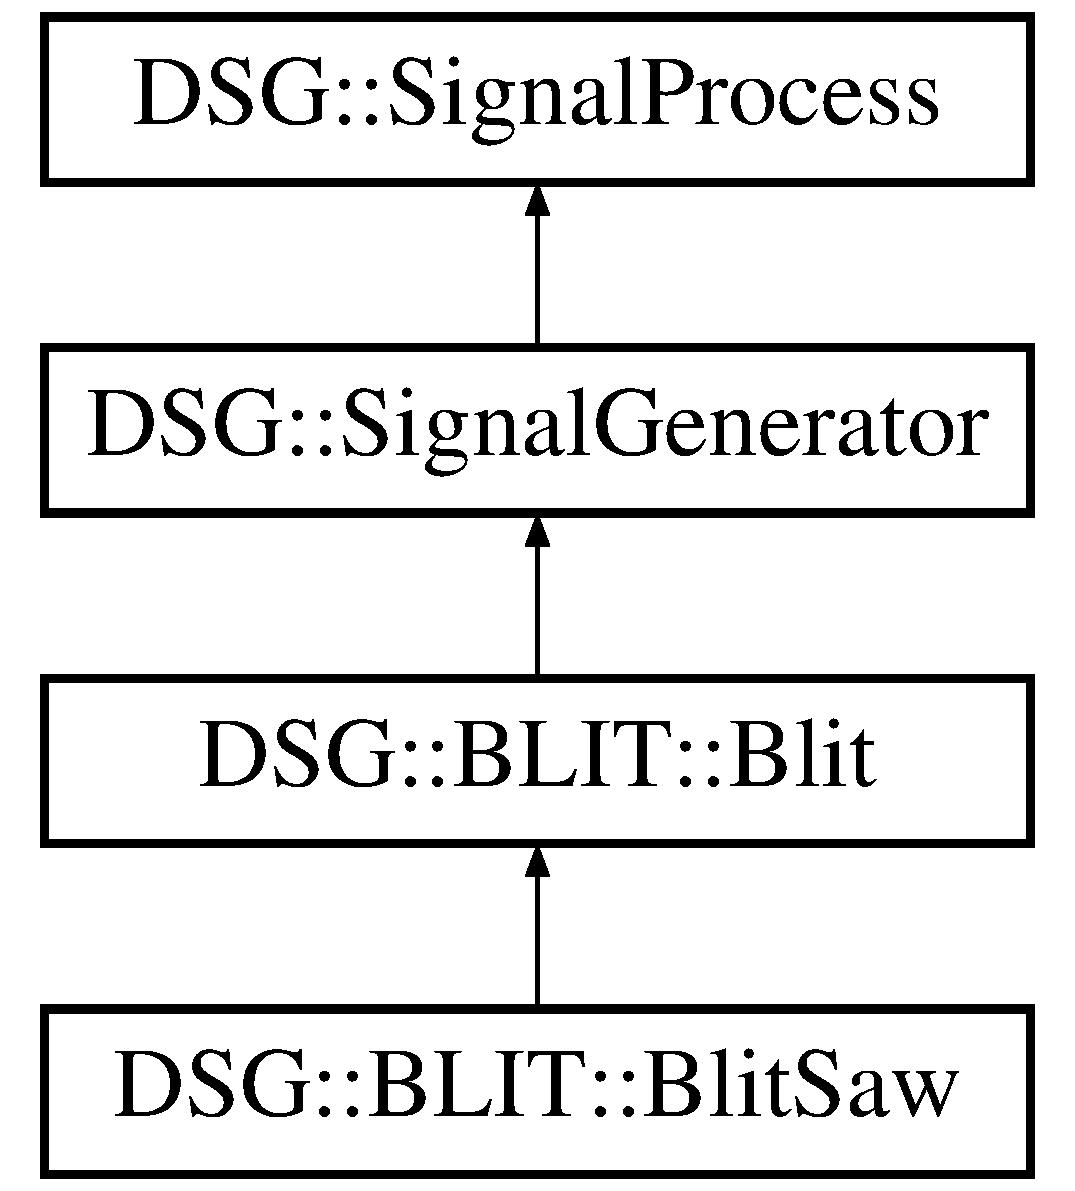
\includegraphics[height=4.000000cm]{class_d_s_g_1_1_b_l_i_t_1_1_blit}
\end{center}
\end{figure}
\subsection*{Public Member Functions}
\begin{DoxyCompactItemize}
\item 
\hyperlink{class_d_s_g_1_1_b_l_i_t_1_1_blit_a1d9bed6285a8b3c0e073f3e3662716af}{Blit} ()
\item 
\hyperlink{class_d_s_g_1_1_b_l_i_t_1_1_blit_a8ab0fb1b908d641527bb86a81d1722ba}{Blit} (\hyperlink{namespace_d_s_g_a4315a061386fa1014fda09b15d3a6973}{D\+S\+G\+::\+D\+S\+G\+Frequency} const \&frequency, \hyperlink{namespace_d_s_g_a44431ce1eb0a7300efdd207bc879e52c}{D\+S\+G\+::\+D\+S\+G\+Phase} const \&offset)
\item 
virtual \hyperlink{class_d_s_g_1_1_b_l_i_t_1_1_blit_a92da2e1763735b3e17f7b9a24377f988}{$\sim$\+Blit} ()
\item 
virtual bool \hyperlink{class_d_s_g_1_1_b_l_i_t_1_1_blit_adfd7c8891b4c4dbd0530a2780781b2bd}{Perform} (\hyperlink{namespace_d_s_g_ac39a94cd27ebcd9c1e7502d0c624894a}{D\+S\+G\+::\+D\+S\+G\+Sample} \&signal)
\item 
virtual bool \hyperlink{class_d_s_g_1_1_b_l_i_t_1_1_blit_aab7c67ff8f059c8367ba316cf8cd5436}{Perform} (\hyperlink{class_d_s_g_1_1_ring_buffer}{D\+S\+G\+::\+Ring\+Buffer} \&signal)
\item 
virtual \hyperlink{namespace_d_s_g_a4315a061386fa1014fda09b15d3a6973}{D\+S\+G\+::\+D\+S\+G\+Frequency} const \& \hyperlink{class_d_s_g_1_1_b_l_i_t_1_1_blit_a933f8f9f324a4fde4f9e2b69473d88ed}{Frequency} (\hyperlink{namespace_d_s_g_a4315a061386fa1014fda09b15d3a6973}{D\+S\+G\+::\+D\+S\+G\+Frequency} const \&\hyperlink{class_d_s_g_1_1_b_l_i_t_1_1_blit_ac8fb9d4fb45d0697bf364bb5d6b570ce}{value})
\end{DoxyCompactItemize}
\subsection*{Protected Attributes}
\begin{DoxyCompactItemize}
\item 
unsigned long \hyperlink{class_d_s_g_1_1_b_l_i_t_1_1_blit_a04d7d6b22a386428e5c25668e1587794}{p\+\_\+}
\item 
unsigned long \hyperlink{class_d_s_g_1_1_b_l_i_t_1_1_blit_afa6e4d46efdbfa032762610601ed42a0}{m\+\_\+}
\item 
unsigned long \hyperlink{class_d_s_g_1_1_b_l_i_t_1_1_blit_a632c6f070187969b90c70b65668b82bc}{\+\_\+h}
\item 
double \hyperlink{class_d_s_g_1_1_b_l_i_t_1_1_blit_a66e2a97840ad0772daaaa9aea63b77b4}{a\+\_\+}
\item 
\hyperlink{namespace_d_s_g_ac39a94cd27ebcd9c1e7502d0c624894a}{D\+S\+G\+::\+D\+S\+G\+Sample} \hyperlink{class_d_s_g_1_1_b_l_i_t_1_1_blit_a6de89a5a240f226c940aef97661c9cee}{denominator}
\item 
\hyperlink{namespace_d_s_g_ac39a94cd27ebcd9c1e7502d0c624894a}{D\+S\+G\+::\+D\+S\+G\+Sample} \hyperlink{class_d_s_g_1_1_b_l_i_t_1_1_blit_ac8fb9d4fb45d0697bf364bb5d6b570ce}{value}
\end{DoxyCompactItemize}
\subsection*{Additional Inherited Members}


\subsection{Detailed Description}
\hyperlink{class_d_s_g_1_1_b_l_i_t_1_1_blit}{D\+S\+G\+::\+B\+L\+I\+T\+::\+Blit} -\/ Band-\/\+Limited Impulse Train Generator. 

\begin{DoxyRefDesc}{Todo}
\item[\hyperlink{todo__todo000001}{Todo}]Re-\/write \hyperlink{class_d_s_g_1_1_b_l_i_t_1_1_blit}{D\+S\+G\+::\+B\+L\+I\+T\+::\+Blit} algorithm \end{DoxyRefDesc}


Definition at line \hyperlink{_b_l_i_t_8h_source_l00039}{39} of file \hyperlink{_b_l_i_t_8h_source}{B\+L\+I\+T.\+h}.



\subsection{Constructor \& Destructor Documentation}
\hypertarget{class_d_s_g_1_1_b_l_i_t_1_1_blit_a1d9bed6285a8b3c0e073f3e3662716af}{\index{D\+S\+G\+::\+B\+L\+I\+T\+::\+Blit@{D\+S\+G\+::\+B\+L\+I\+T\+::\+Blit}!Blit@{Blit}}
\index{Blit@{Blit}!D\+S\+G\+::\+B\+L\+I\+T\+::\+Blit@{D\+S\+G\+::\+B\+L\+I\+T\+::\+Blit}}
\subsubsection[{Blit}]{\setlength{\rightskip}{0pt plus 5cm}D\+S\+G\+::\+B\+L\+I\+T\+::\+Blit\+::\+Blit (
\begin{DoxyParamCaption}
{}
\end{DoxyParamCaption}
)}}\label{class_d_s_g_1_1_b_l_i_t_1_1_blit_a1d9bed6285a8b3c0e073f3e3662716af}


Definition at line \hyperlink{_b_l_i_t_8cpp_source_l00025}{25} of file \hyperlink{_b_l_i_t_8cpp_source}{B\+L\+I\+T.\+cpp}.


\begin{DoxyCode}
00025                  :\hyperlink{class_d_s_g_1_1_signal_generator}{DSG::SignalGenerator}()\{
00026     \hyperlink{class_d_s_g_1_1_phasor_a6bdec1d2722e2fa5c7173ac5f7adf682}{Frequency}(0);
00027 \}
\end{DoxyCode}
\hypertarget{class_d_s_g_1_1_b_l_i_t_1_1_blit_a8ab0fb1b908d641527bb86a81d1722ba}{\index{D\+S\+G\+::\+B\+L\+I\+T\+::\+Blit@{D\+S\+G\+::\+B\+L\+I\+T\+::\+Blit}!Blit@{Blit}}
\index{Blit@{Blit}!D\+S\+G\+::\+B\+L\+I\+T\+::\+Blit@{D\+S\+G\+::\+B\+L\+I\+T\+::\+Blit}}
\subsubsection[{Blit}]{\setlength{\rightskip}{0pt plus 5cm}D\+S\+G\+::\+B\+L\+I\+T\+::\+Blit\+::\+Blit (
\begin{DoxyParamCaption}
\item[{{\bf D\+S\+G\+::\+D\+S\+G\+Frequency} const \&}]{frequency, }
\item[{{\bf D\+S\+G\+::\+D\+S\+G\+Phase} const \&}]{offset}
\end{DoxyParamCaption}
)}}\label{class_d_s_g_1_1_b_l_i_t_1_1_blit_a8ab0fb1b908d641527bb86a81d1722ba}


Definition at line \hyperlink{_b_l_i_t_8cpp_source_l00028}{28} of file \hyperlink{_b_l_i_t_8cpp_source}{B\+L\+I\+T.\+cpp}.


\begin{DoxyCode}
00028                                                                            :
      \hyperlink{class_d_s_g_1_1_signal_generator}{DSG::SignalGenerator}(frequency,offset)\{
00029     \hyperlink{class_d_s_g_1_1_phasor_a6bdec1d2722e2fa5c7173ac5f7adf682}{Frequency}(frequency);
00030 \}
\end{DoxyCode}
\hypertarget{class_d_s_g_1_1_b_l_i_t_1_1_blit_a92da2e1763735b3e17f7b9a24377f988}{\index{D\+S\+G\+::\+B\+L\+I\+T\+::\+Blit@{D\+S\+G\+::\+B\+L\+I\+T\+::\+Blit}!````~Blit@{$\sim$\+Blit}}
\index{````~Blit@{$\sim$\+Blit}!D\+S\+G\+::\+B\+L\+I\+T\+::\+Blit@{D\+S\+G\+::\+B\+L\+I\+T\+::\+Blit}}
\subsubsection[{$\sim$\+Blit}]{\setlength{\rightskip}{0pt plus 5cm}D\+S\+G\+::\+B\+L\+I\+T\+::\+Blit\+::$\sim$\+Blit (
\begin{DoxyParamCaption}
{}
\end{DoxyParamCaption}
)\hspace{0.3cm}{\ttfamily [virtual]}}}\label{class_d_s_g_1_1_b_l_i_t_1_1_blit_a92da2e1763735b3e17f7b9a24377f988}


Definition at line \hyperlink{_b_l_i_t_8cpp_source_l00031}{31} of file \hyperlink{_b_l_i_t_8cpp_source}{B\+L\+I\+T.\+cpp}.


\begin{DoxyCode}
00031 \{\}\end{DoxyCode}


\subsection{Member Function Documentation}
\hypertarget{class_d_s_g_1_1_b_l_i_t_1_1_blit_a933f8f9f324a4fde4f9e2b69473d88ed}{\index{D\+S\+G\+::\+B\+L\+I\+T\+::\+Blit@{D\+S\+G\+::\+B\+L\+I\+T\+::\+Blit}!Frequency@{Frequency}}
\index{Frequency@{Frequency}!D\+S\+G\+::\+B\+L\+I\+T\+::\+Blit@{D\+S\+G\+::\+B\+L\+I\+T\+::\+Blit}}
\subsubsection[{Frequency}]{\setlength{\rightskip}{0pt plus 5cm}{\bf D\+S\+G\+::\+D\+S\+G\+Frequency} const \& D\+S\+G\+::\+B\+L\+I\+T\+::\+Blit\+::\+Frequency (
\begin{DoxyParamCaption}
\item[{{\bf D\+S\+G\+::\+D\+S\+G\+Frequency} const \&}]{value}
\end{DoxyParamCaption}
)\hspace{0.3cm}{\ttfamily [inline]}, {\ttfamily [virtual]}}}\label{class_d_s_g_1_1_b_l_i_t_1_1_blit_a933f8f9f324a4fde4f9e2b69473d88ed}


Reimplemented from \hyperlink{class_d_s_g_1_1_phasor_a8162456ae44291008159acd89bfa7b1b}{D\+S\+G\+::\+Phasor}.



Reimplemented in \hyperlink{class_d_s_g_1_1_b_l_i_t_1_1_blit_saw_a290d01796efca84b73eb61a3bc419ebb}{D\+S\+G\+::\+B\+L\+I\+T\+::\+Blit\+Saw}.



Definition at line \hyperlink{_b_l_i_t_8h_source_l00078}{78} of file \hyperlink{_b_l_i_t_8h_source}{B\+L\+I\+T.\+h}.


\begin{DoxyCode}
00078                                                                                         \{
00079             this->\hyperlink{class_d_s_g_1_1_phasor_a6bdec1d2722e2fa5c7173ac5f7adf682}{SignalGenerator::Frequency}(\hyperlink{class_d_s_g_1_1_b_l_i_t_1_1_blit_ac8fb9d4fb45d0697bf364bb5d6b570ce}{value});
00080             \hyperlink{class_d_s_g_1_1_b_l_i_t_1_1_blit_a04d7d6b22a386428e5c25668e1587794}{p\_} = \hyperlink{namespace_d_s_g_a72df05177db0412c3590070923f62819}{DSG::SampleRate}()/\hyperlink{class_d_s_g_1_1_phasor_a85a00065d4445c33fef69eae0ce926df}{\_frequency};
00081             \hyperlink{class_d_s_g_1_1_b_l_i_t_1_1_blit_a632c6f070187969b90c70b65668b82bc}{\_h} = (unsigned)floor(\hyperlink{class_d_s_g_1_1_b_l_i_t_1_1_blit_a04d7d6b22a386428e5c25668e1587794}{p\_}*0.5);
00082             \hyperlink{class_d_s_g_1_1_b_l_i_t_1_1_blit_afa6e4d46efdbfa032762610601ed42a0}{m\_} = 2 * (\hyperlink{class_d_s_g_1_1_b_l_i_t_1_1_blit_a632c6f070187969b90c70b65668b82bc}{\_h})+1;
00083             \hyperlink{class_d_s_g_1_1_b_l_i_t_1_1_blit_a66e2a97840ad0772daaaa9aea63b77b4}{a\_} = \hyperlink{class_d_s_g_1_1_b_l_i_t_1_1_blit_afa6e4d46efdbfa032762610601ed42a0}{m\_}/(double)\hyperlink{class_d_s_g_1_1_b_l_i_t_1_1_blit_a04d7d6b22a386428e5c25668e1587794}{p\_};
00084             \textcolor{keywordflow}{return} \hyperlink{class_d_s_g_1_1_phasor_a85a00065d4445c33fef69eae0ce926df}{\_frequency};
00085         \}
\end{DoxyCode}
\hypertarget{class_d_s_g_1_1_b_l_i_t_1_1_blit_adfd7c8891b4c4dbd0530a2780781b2bd}{\index{D\+S\+G\+::\+B\+L\+I\+T\+::\+Blit@{D\+S\+G\+::\+B\+L\+I\+T\+::\+Blit}!Perform@{Perform}}
\index{Perform@{Perform}!D\+S\+G\+::\+B\+L\+I\+T\+::\+Blit@{D\+S\+G\+::\+B\+L\+I\+T\+::\+Blit}}
\subsubsection[{Perform}]{\setlength{\rightskip}{0pt plus 5cm}bool D\+S\+G\+::\+B\+L\+I\+T\+::\+Blit\+::\+Perform (
\begin{DoxyParamCaption}
\item[{{\bf D\+S\+G\+::\+D\+S\+G\+Sample} \&}]{signal}
\end{DoxyParamCaption}
)\hspace{0.3cm}{\ttfamily [inline]}, {\ttfamily [virtual]}}}\label{class_d_s_g_1_1_b_l_i_t_1_1_blit_adfd7c8891b4c4dbd0530a2780781b2bd}


Reimplemented from \hyperlink{class_d_s_g_1_1_signal_generator_a46fe75a81a242e191c5049d33ddf4155}{D\+S\+G\+::\+Signal\+Generator}.



Reimplemented in \hyperlink{class_d_s_g_1_1_b_l_i_t_1_1_blit_saw_ae24821c51b23b9fe9220a620e558af04}{D\+S\+G\+::\+B\+L\+I\+T\+::\+Blit\+Saw}.



Definition at line \hyperlink{_b_l_i_t_8h_source_l00055}{55} of file \hyperlink{_b_l_i_t_8h_source}{B\+L\+I\+T.\+h}.


\begin{DoxyCode}
00055                                                             \{
00056             \textcolor{comment}{//found better results in this case with built in sine function. not performance wise but
       algorithmically}
00057             \hyperlink{class_d_s_g_1_1_b_l_i_t_1_1_blit_a6de89a5a240f226c940aef97661c9cee}{denominator} = \hyperlink{class_d_s_g_1_1_b_l_i_t_1_1_blit_afa6e4d46efdbfa032762610601ed42a0}{m\_} * sin(\hyperlink{class_d_s_g_1_1_phasor_a82c148d71128cfc518fc8e7e131c3a38}{\_phasor});
00058             \textcolor{keywordflow}{if} (\hyperlink{namespace_d_s_g_a9eee3c39a1f45d42f0b4fa7201d3ba3d}{DSG::IsDenormal}(\hyperlink{class_d_s_g_1_1_b_l_i_t_1_1_blit_a6de89a5a240f226c940aef97661c9cee}{denominator})) \{
00059                 signal = \hyperlink{class_d_s_g_1_1_b_l_i_t_1_1_blit_a66e2a97840ad0772daaaa9aea63b77b4}{a\_};
00060             \}\textcolor{keywordflow}{else}\{
00061                 \hyperlink{class_d_s_g_1_1_b_l_i_t_1_1_blit_ac8fb9d4fb45d0697bf364bb5d6b570ce}{value} = sin(\hyperlink{_p_i_8h_a598a3330b3c21701223ee0ca14316eca}{PI}*\hyperlink{class_d_s_g_1_1_phasor_a82c148d71128cfc518fc8e7e131c3a38}{\_phasor} * \hyperlink{class_d_s_g_1_1_b_l_i_t_1_1_blit_afa6e4d46efdbfa032762610601ed42a0}{m\_});
00062                 \hyperlink{class_d_s_g_1_1_b_l_i_t_1_1_blit_ac8fb9d4fb45d0697bf364bb5d6b570ce}{value}/=\hyperlink{class_d_s_g_1_1_b_l_i_t_1_1_blit_a6de89a5a240f226c940aef97661c9cee}{denominator};
00063                 \hyperlink{class_d_s_g_1_1_b_l_i_t_1_1_blit_ac8fb9d4fb45d0697bf364bb5d6b570ce}{value}*=\hyperlink{class_d_s_g_1_1_b_l_i_t_1_1_blit_a66e2a97840ad0772daaaa9aea63b77b4}{a\_};
00064                 signal = \hyperlink{class_d_s_g_1_1_b_l_i_t_1_1_blit_ac8fb9d4fb45d0697bf364bb5d6b570ce}{value};
00065             \}
00066             \hyperlink{class_d_s_g_1_1_phasor_a6a088b29e506fb5e99d73f4f0160c583}{step}();
00067             \textcolor{keywordflow}{return} \textcolor{keyword}{true};
00068         \}
\end{DoxyCode}
\hypertarget{class_d_s_g_1_1_b_l_i_t_1_1_blit_aab7c67ff8f059c8367ba316cf8cd5436}{\index{D\+S\+G\+::\+B\+L\+I\+T\+::\+Blit@{D\+S\+G\+::\+B\+L\+I\+T\+::\+Blit}!Perform@{Perform}}
\index{Perform@{Perform}!D\+S\+G\+::\+B\+L\+I\+T\+::\+Blit@{D\+S\+G\+::\+B\+L\+I\+T\+::\+Blit}}
\subsubsection[{Perform}]{\setlength{\rightskip}{0pt plus 5cm}bool D\+S\+G\+::\+B\+L\+I\+T\+::\+Blit\+::\+Perform (
\begin{DoxyParamCaption}
\item[{{\bf D\+S\+G\+::\+Ring\+Buffer} \&}]{signal}
\end{DoxyParamCaption}
)\hspace{0.3cm}{\ttfamily [inline]}, {\ttfamily [virtual]}}}\label{class_d_s_g_1_1_b_l_i_t_1_1_blit_aab7c67ff8f059c8367ba316cf8cd5436}


Reimplemented from \hyperlink{class_d_s_g_1_1_signal_generator_ab050f80e84e6c8b3e354b56930d6a02b}{D\+S\+G\+::\+Signal\+Generator}.



Reimplemented in \hyperlink{class_d_s_g_1_1_b_l_i_t_1_1_blit_saw_ad2edba8ed83558e76afed6ec1d5cf4d6}{D\+S\+G\+::\+B\+L\+I\+T\+::\+Blit\+Saw}.



Definition at line \hyperlink{_b_l_i_t_8h_source_l00069}{69} of file \hyperlink{_b_l_i_t_8h_source}{B\+L\+I\+T.\+h}.


\begin{DoxyCode}
00069                                                              \{
00070             signal.\hyperlink{class_d_s_g_1_1_ring_buffer_ab23c8003d2857809a816068eeb209d60}{Flush}();
00071             \textcolor{keywordflow}{while} (!signal.\hyperlink{class_d_s_g_1_1_ring_buffer_a53ddb04ffcbb5470a8d2b0a3c65b70cb}{Full}()) \{
00072                 \textcolor{keywordflow}{if} (\hyperlink{class_d_s_g_1_1_b_l_i_t_1_1_blit_adfd7c8891b4c4dbd0530a2780781b2bd}{Perform}(\hyperlink{class_d_s_g_1_1_signal_generator_a28a9b47a1aa0783029f11a19ba0363f2}{\_storage})) \{
00073                     \textcolor{keywordflow}{if}(signal.\hyperlink{class_d_s_g_1_1_ring_buffer_aa5dd2caa0a270173251faee40a43d692}{Write}(\hyperlink{class_d_s_g_1_1_signal_generator_a28a9b47a1aa0783029f11a19ba0363f2}{\_storage}))\{
00074                     \}\textcolor{keywordflow}{else} \textcolor{keywordflow}{return} \textcolor{keyword}{false};
00075                 \}\textcolor{keywordflow}{else} \textcolor{keywordflow}{return} \textcolor{keyword}{false};
00076             \}\textcolor{keywordflow}{return} \textcolor{keyword}{true};
00077         \}
\end{DoxyCode}


\subsection{Member Data Documentation}
\hypertarget{class_d_s_g_1_1_b_l_i_t_1_1_blit_a632c6f070187969b90c70b65668b82bc}{\index{D\+S\+G\+::\+B\+L\+I\+T\+::\+Blit@{D\+S\+G\+::\+B\+L\+I\+T\+::\+Blit}!\+\_\+h@{\+\_\+h}}
\index{\+\_\+h@{\+\_\+h}!D\+S\+G\+::\+B\+L\+I\+T\+::\+Blit@{D\+S\+G\+::\+B\+L\+I\+T\+::\+Blit}}
\subsubsection[{\+\_\+h}]{\setlength{\rightskip}{0pt plus 5cm}unsigned long D\+S\+G\+::\+B\+L\+I\+T\+::\+Blit\+::\+\_\+h\hspace{0.3cm}{\ttfamily [protected]}}}\label{class_d_s_g_1_1_b_l_i_t_1_1_blit_a632c6f070187969b90c70b65668b82bc}


Definition at line \hyperlink{_b_l_i_t_8h_source_l00050}{50} of file \hyperlink{_b_l_i_t_8h_source}{B\+L\+I\+T.\+h}.

\hypertarget{class_d_s_g_1_1_b_l_i_t_1_1_blit_a66e2a97840ad0772daaaa9aea63b77b4}{\index{D\+S\+G\+::\+B\+L\+I\+T\+::\+Blit@{D\+S\+G\+::\+B\+L\+I\+T\+::\+Blit}!a\+\_\+@{a\+\_\+}}
\index{a\+\_\+@{a\+\_\+}!D\+S\+G\+::\+B\+L\+I\+T\+::\+Blit@{D\+S\+G\+::\+B\+L\+I\+T\+::\+Blit}}
\subsubsection[{a\+\_\+}]{\setlength{\rightskip}{0pt plus 5cm}double D\+S\+G\+::\+B\+L\+I\+T\+::\+Blit\+::a\+\_\+\hspace{0.3cm}{\ttfamily [protected]}}}\label{class_d_s_g_1_1_b_l_i_t_1_1_blit_a66e2a97840ad0772daaaa9aea63b77b4}


Definition at line \hyperlink{_b_l_i_t_8h_source_l00051}{51} of file \hyperlink{_b_l_i_t_8h_source}{B\+L\+I\+T.\+h}.

\hypertarget{class_d_s_g_1_1_b_l_i_t_1_1_blit_a6de89a5a240f226c940aef97661c9cee}{\index{D\+S\+G\+::\+B\+L\+I\+T\+::\+Blit@{D\+S\+G\+::\+B\+L\+I\+T\+::\+Blit}!denominator@{denominator}}
\index{denominator@{denominator}!D\+S\+G\+::\+B\+L\+I\+T\+::\+Blit@{D\+S\+G\+::\+B\+L\+I\+T\+::\+Blit}}
\subsubsection[{denominator}]{\setlength{\rightskip}{0pt plus 5cm}{\bf D\+S\+G\+::\+D\+S\+G\+Sample} D\+S\+G\+::\+B\+L\+I\+T\+::\+Blit\+::denominator\hspace{0.3cm}{\ttfamily [protected]}}}\label{class_d_s_g_1_1_b_l_i_t_1_1_blit_a6de89a5a240f226c940aef97661c9cee}


Definition at line \hyperlink{_b_l_i_t_8h_source_l00052}{52} of file \hyperlink{_b_l_i_t_8h_source}{B\+L\+I\+T.\+h}.

\hypertarget{class_d_s_g_1_1_b_l_i_t_1_1_blit_afa6e4d46efdbfa032762610601ed42a0}{\index{D\+S\+G\+::\+B\+L\+I\+T\+::\+Blit@{D\+S\+G\+::\+B\+L\+I\+T\+::\+Blit}!m\+\_\+@{m\+\_\+}}
\index{m\+\_\+@{m\+\_\+}!D\+S\+G\+::\+B\+L\+I\+T\+::\+Blit@{D\+S\+G\+::\+B\+L\+I\+T\+::\+Blit}}
\subsubsection[{m\+\_\+}]{\setlength{\rightskip}{0pt plus 5cm}unsigned long D\+S\+G\+::\+B\+L\+I\+T\+::\+Blit\+::m\+\_\+\hspace{0.3cm}{\ttfamily [protected]}}}\label{class_d_s_g_1_1_b_l_i_t_1_1_blit_afa6e4d46efdbfa032762610601ed42a0}


Definition at line \hyperlink{_b_l_i_t_8h_source_l00049}{49} of file \hyperlink{_b_l_i_t_8h_source}{B\+L\+I\+T.\+h}.

\hypertarget{class_d_s_g_1_1_b_l_i_t_1_1_blit_a04d7d6b22a386428e5c25668e1587794}{\index{D\+S\+G\+::\+B\+L\+I\+T\+::\+Blit@{D\+S\+G\+::\+B\+L\+I\+T\+::\+Blit}!p\+\_\+@{p\+\_\+}}
\index{p\+\_\+@{p\+\_\+}!D\+S\+G\+::\+B\+L\+I\+T\+::\+Blit@{D\+S\+G\+::\+B\+L\+I\+T\+::\+Blit}}
\subsubsection[{p\+\_\+}]{\setlength{\rightskip}{0pt plus 5cm}unsigned long D\+S\+G\+::\+B\+L\+I\+T\+::\+Blit\+::p\+\_\+\hspace{0.3cm}{\ttfamily [protected]}}}\label{class_d_s_g_1_1_b_l_i_t_1_1_blit_a04d7d6b22a386428e5c25668e1587794}


Definition at line \hyperlink{_b_l_i_t_8h_source_l00048}{48} of file \hyperlink{_b_l_i_t_8h_source}{B\+L\+I\+T.\+h}.

\hypertarget{class_d_s_g_1_1_b_l_i_t_1_1_blit_ac8fb9d4fb45d0697bf364bb5d6b570ce}{\index{D\+S\+G\+::\+B\+L\+I\+T\+::\+Blit@{D\+S\+G\+::\+B\+L\+I\+T\+::\+Blit}!value@{value}}
\index{value@{value}!D\+S\+G\+::\+B\+L\+I\+T\+::\+Blit@{D\+S\+G\+::\+B\+L\+I\+T\+::\+Blit}}
\subsubsection[{value}]{\setlength{\rightskip}{0pt plus 5cm}{\bf D\+S\+G\+::\+D\+S\+G\+Sample} D\+S\+G\+::\+B\+L\+I\+T\+::\+Blit\+::value\hspace{0.3cm}{\ttfamily [protected]}}}\label{class_d_s_g_1_1_b_l_i_t_1_1_blit_ac8fb9d4fb45d0697bf364bb5d6b570ce}


Definition at line \hyperlink{_b_l_i_t_8h_source_l00053}{53} of file \hyperlink{_b_l_i_t_8h_source}{B\+L\+I\+T.\+h}.



The documentation for this class was generated from the following files\+:\begin{DoxyCompactItemize}
\item 
\hyperlink{_b_l_i_t_8h}{B\+L\+I\+T.\+h}\item 
\hyperlink{_b_l_i_t_8cpp}{B\+L\+I\+T.\+cpp}\end{DoxyCompactItemize}

\hypertarget{class_d_s_g_1_1_b_l_i_t_1_1_blit_saw}{\section{D\+S\+G\+:\+:B\+L\+I\+T\+:\+:Blit\+Saw Class Reference}
\label{class_d_s_g_1_1_b_l_i_t_1_1_blit_saw}\index{D\+S\+G\+::\+B\+L\+I\+T\+::\+Blit\+Saw@{D\+S\+G\+::\+B\+L\+I\+T\+::\+Blit\+Saw}}
}


\hyperlink{class_d_s_g_1_1_b_l_i_t_1_1_blit_saw}{D\+S\+G\+::\+B\+L\+I\+T\+::\+Blit\+Saw} -\/ Saw Wave Generator Based on \hyperlink{namespace_d_s_g_1_1_b_l_i_t}{B\+L\+I\+T} Algorithm.  




{\ttfamily \#include $<$B\+L\+I\+T\+Saw.\+h$>$}

Inheritance diagram for D\+S\+G\+:\+:B\+L\+I\+T\+:\+:Blit\+Saw\+:\begin{figure}[H]
\begin{center}
\leavevmode
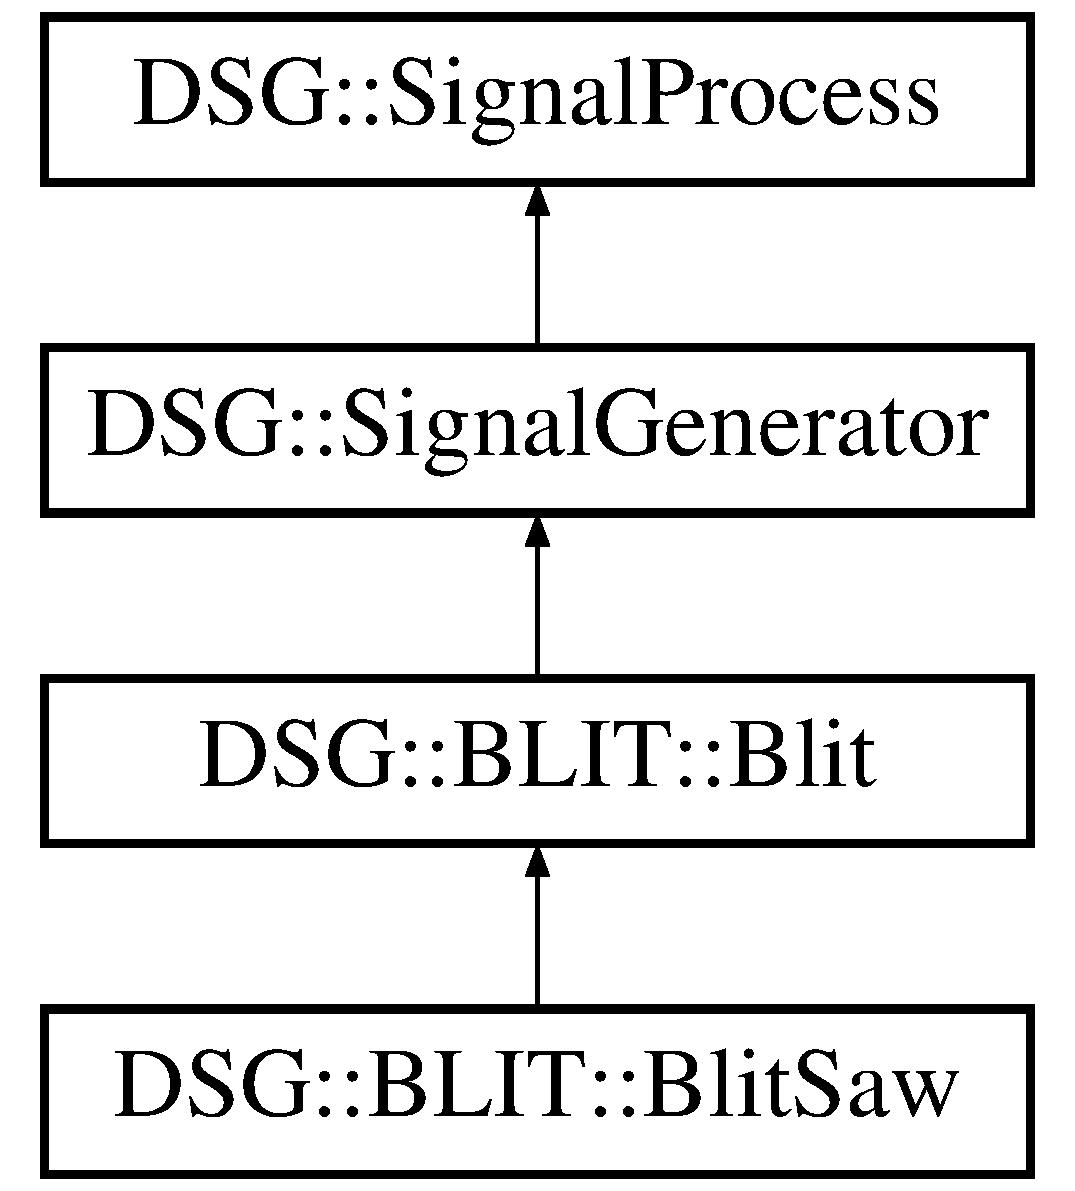
\includegraphics[height=4.000000cm]{class_d_s_g_1_1_b_l_i_t_1_1_blit_saw}
\end{center}
\end{figure}
\subsection*{Public Member Functions}
\begin{DoxyCompactItemize}
\item 
\hyperlink{class_d_s_g_1_1_b_l_i_t_1_1_blit_saw_a5c73a4aeb4df74da4db4896edeb15059}{Blit\+Saw} ()
\item 
\hyperlink{class_d_s_g_1_1_b_l_i_t_1_1_blit_saw_a3d7e4379c00970fa89085ed2c945a2b7}{Blit\+Saw} (\hyperlink{namespace_d_s_g_a4315a061386fa1014fda09b15d3a6973}{D\+S\+G\+::\+D\+S\+G\+Frequency} const \&frequency, \hyperlink{namespace_d_s_g_a44431ce1eb0a7300efdd207bc879e52c}{D\+S\+G\+::\+D\+S\+G\+Phase} const \&offset)
\item 
virtual \hyperlink{class_d_s_g_1_1_b_l_i_t_1_1_blit_saw_a4744c63b29aee896823f19965e11e515}{$\sim$\+Blit\+Saw} ()
\item 
virtual bool \hyperlink{class_d_s_g_1_1_b_l_i_t_1_1_blit_saw_ae24821c51b23b9fe9220a620e558af04}{Perform} (\hyperlink{namespace_d_s_g_ac39a94cd27ebcd9c1e7502d0c624894a}{D\+S\+G\+::\+D\+S\+G\+Sample} \&signal)
\item 
virtual bool \hyperlink{class_d_s_g_1_1_b_l_i_t_1_1_blit_saw_ad2edba8ed83558e76afed6ec1d5cf4d6}{Perform} (\hyperlink{class_d_s_g_1_1_ring_buffer}{D\+S\+G\+::\+Ring\+Buffer} \&signal)
\item 
virtual \hyperlink{namespace_d_s_g_a4315a061386fa1014fda09b15d3a6973}{D\+S\+G\+::\+D\+S\+G\+Frequency} const \& \hyperlink{class_d_s_g_1_1_b_l_i_t_1_1_blit_saw_a290d01796efca84b73eb61a3bc419ebb}{Frequency} (\hyperlink{namespace_d_s_g_a4315a061386fa1014fda09b15d3a6973}{D\+S\+G\+::\+D\+S\+G\+Frequency} const \&\hyperlink{class_d_s_g_1_1_b_l_i_t_1_1_blit_ac8fb9d4fb45d0697bf364bb5d6b570ce}{value})
\end{DoxyCompactItemize}
\subsection*{Protected Attributes}
\begin{DoxyCompactItemize}
\item 
\hyperlink{namespace_d_s_g_ac39a94cd27ebcd9c1e7502d0c624894a}{D\+S\+G\+::\+D\+S\+G\+Sample} \hyperlink{class_d_s_g_1_1_b_l_i_t_1_1_blit_saw_a39ff301ab1f690c070b2045d4a2c40bf}{C2\+\_\+}
\item 
\hyperlink{namespace_d_s_g_ac39a94cd27ebcd9c1e7502d0c624894a}{D\+S\+G\+::\+D\+S\+G\+Sample} \hyperlink{class_d_s_g_1_1_b_l_i_t_1_1_blit_saw_a15da9acffc369dd3c5233c05d37ee488}{Register\+\_\+}
\end{DoxyCompactItemize}
\subsection*{Additional Inherited Members}


\subsection{Detailed Description}
\hyperlink{class_d_s_g_1_1_b_l_i_t_1_1_blit_saw}{D\+S\+G\+::\+B\+L\+I\+T\+::\+Blit\+Saw} -\/ Saw Wave Generator Based on \hyperlink{namespace_d_s_g_1_1_b_l_i_t}{B\+L\+I\+T} Algorithm. 

\begin{DoxyRefDesc}{Todo}
\item[\hyperlink{todo__todo000002}{Todo}]Re-\/write \hyperlink{class_d_s_g_1_1_b_l_i_t_1_1_blit_saw}{D\+S\+G\+::\+B\+L\+I\+T\+::\+Blit\+Saw} algorithm \end{DoxyRefDesc}


Definition at line \hyperlink{_b_l_i_t_saw_8h_source_l00034}{34} of file \hyperlink{_b_l_i_t_saw_8h_source}{B\+L\+I\+T\+Saw.\+h}.



\subsection{Constructor \& Destructor Documentation}
\hypertarget{class_d_s_g_1_1_b_l_i_t_1_1_blit_saw_a5c73a4aeb4df74da4db4896edeb15059}{\index{D\+S\+G\+::\+B\+L\+I\+T\+::\+Blit\+Saw@{D\+S\+G\+::\+B\+L\+I\+T\+::\+Blit\+Saw}!Blit\+Saw@{Blit\+Saw}}
\index{Blit\+Saw@{Blit\+Saw}!D\+S\+G\+::\+B\+L\+I\+T\+::\+Blit\+Saw@{D\+S\+G\+::\+B\+L\+I\+T\+::\+Blit\+Saw}}
\subsubsection[{Blit\+Saw}]{\setlength{\rightskip}{0pt plus 5cm}D\+S\+G\+::\+B\+L\+I\+T\+::\+Blit\+Saw\+::\+Blit\+Saw (
\begin{DoxyParamCaption}
{}
\end{DoxyParamCaption}
)}}\label{class_d_s_g_1_1_b_l_i_t_1_1_blit_saw_a5c73a4aeb4df74da4db4896edeb15059}


Definition at line \hyperlink{_b_l_i_t_saw_8cpp_source_l00025}{25} of file \hyperlink{_b_l_i_t_saw_8cpp_source}{B\+L\+I\+T\+Saw.\+cpp}.


\begin{DoxyCode}
00025                        :\hyperlink{class_d_s_g_1_1_b_l_i_t_1_1_blit}{DSG::BLIT::Blit}(),\hyperlink{class_d_s_g_1_1_b_l_i_t_1_1_blit_saw_a15da9acffc369dd3c5233c05d37ee488}{Register\_}(0)\{
00026     \hyperlink{class_d_s_g_1_1_phasor_a6bdec1d2722e2fa5c7173ac5f7adf682}{Frequency}(0);
00027 \}
\end{DoxyCode}
\hypertarget{class_d_s_g_1_1_b_l_i_t_1_1_blit_saw_a3d7e4379c00970fa89085ed2c945a2b7}{\index{D\+S\+G\+::\+B\+L\+I\+T\+::\+Blit\+Saw@{D\+S\+G\+::\+B\+L\+I\+T\+::\+Blit\+Saw}!Blit\+Saw@{Blit\+Saw}}
\index{Blit\+Saw@{Blit\+Saw}!D\+S\+G\+::\+B\+L\+I\+T\+::\+Blit\+Saw@{D\+S\+G\+::\+B\+L\+I\+T\+::\+Blit\+Saw}}
\subsubsection[{Blit\+Saw}]{\setlength{\rightskip}{0pt plus 5cm}D\+S\+G\+::\+B\+L\+I\+T\+::\+Blit\+Saw\+::\+Blit\+Saw (
\begin{DoxyParamCaption}
\item[{{\bf D\+S\+G\+::\+D\+S\+G\+Frequency} const \&}]{frequency, }
\item[{{\bf D\+S\+G\+::\+D\+S\+G\+Phase} const \&}]{offset}
\end{DoxyParamCaption}
)}}\label{class_d_s_g_1_1_b_l_i_t_1_1_blit_saw_a3d7e4379c00970fa89085ed2c945a2b7}


Definition at line \hyperlink{_b_l_i_t_saw_8cpp_source_l00028}{28} of file \hyperlink{_b_l_i_t_saw_8cpp_source}{B\+L\+I\+T\+Saw.\+cpp}.


\begin{DoxyCode}
00028                                                                                  :
      \hyperlink{class_d_s_g_1_1_b_l_i_t_1_1_blit}{DSG::BLIT::Blit}(frequency,offset),\hyperlink{class_d_s_g_1_1_b_l_i_t_1_1_blit_saw_a15da9acffc369dd3c5233c05d37ee488}{Register\_}(0)\{
00029     \hyperlink{class_d_s_g_1_1_phasor_a6bdec1d2722e2fa5c7173ac5f7adf682}{Frequency}(frequency);
00030 \}
\end{DoxyCode}
\hypertarget{class_d_s_g_1_1_b_l_i_t_1_1_blit_saw_a4744c63b29aee896823f19965e11e515}{\index{D\+S\+G\+::\+B\+L\+I\+T\+::\+Blit\+Saw@{D\+S\+G\+::\+B\+L\+I\+T\+::\+Blit\+Saw}!````~Blit\+Saw@{$\sim$\+Blit\+Saw}}
\index{````~Blit\+Saw@{$\sim$\+Blit\+Saw}!D\+S\+G\+::\+B\+L\+I\+T\+::\+Blit\+Saw@{D\+S\+G\+::\+B\+L\+I\+T\+::\+Blit\+Saw}}
\subsubsection[{$\sim$\+Blit\+Saw}]{\setlength{\rightskip}{0pt plus 5cm}D\+S\+G\+::\+B\+L\+I\+T\+::\+Blit\+Saw\+::$\sim$\+Blit\+Saw (
\begin{DoxyParamCaption}
{}
\end{DoxyParamCaption}
)\hspace{0.3cm}{\ttfamily [virtual]}}}\label{class_d_s_g_1_1_b_l_i_t_1_1_blit_saw_a4744c63b29aee896823f19965e11e515}


Definition at line \hyperlink{_b_l_i_t_saw_8cpp_source_l00031}{31} of file \hyperlink{_b_l_i_t_saw_8cpp_source}{B\+L\+I\+T\+Saw.\+cpp}.


\begin{DoxyCode}
00031 \{\}\end{DoxyCode}


\subsection{Member Function Documentation}
\hypertarget{class_d_s_g_1_1_b_l_i_t_1_1_blit_saw_a290d01796efca84b73eb61a3bc419ebb}{\index{D\+S\+G\+::\+B\+L\+I\+T\+::\+Blit\+Saw@{D\+S\+G\+::\+B\+L\+I\+T\+::\+Blit\+Saw}!Frequency@{Frequency}}
\index{Frequency@{Frequency}!D\+S\+G\+::\+B\+L\+I\+T\+::\+Blit\+Saw@{D\+S\+G\+::\+B\+L\+I\+T\+::\+Blit\+Saw}}
\subsubsection[{Frequency}]{\setlength{\rightskip}{0pt plus 5cm}{\bf D\+S\+G\+::\+D\+S\+G\+Frequency} const \& D\+S\+G\+::\+B\+L\+I\+T\+::\+Blit\+Saw\+::\+Frequency (
\begin{DoxyParamCaption}
\item[{{\bf D\+S\+G\+::\+D\+S\+G\+Frequency} const \&}]{value}
\end{DoxyParamCaption}
)\hspace{0.3cm}{\ttfamily [inline]}, {\ttfamily [virtual]}}}\label{class_d_s_g_1_1_b_l_i_t_1_1_blit_saw_a290d01796efca84b73eb61a3bc419ebb}


Reimplemented from \hyperlink{class_d_s_g_1_1_b_l_i_t_1_1_blit_a933f8f9f324a4fde4f9e2b69473d88ed}{D\+S\+G\+::\+B\+L\+I\+T\+::\+Blit}.



Definition at line \hyperlink{_b_l_i_t_saw_8h_source_l00072}{72} of file \hyperlink{_b_l_i_t_saw_8h_source}{B\+L\+I\+T\+Saw.\+h}.


\begin{DoxyCode}
00072                                                                                            \{
00073             this->\hyperlink{class_d_s_g_1_1_phasor_a6bdec1d2722e2fa5c7173ac5f7adf682}{SignalGenerator::Frequency}(\hyperlink{class_d_s_g_1_1_b_l_i_t_1_1_blit_ac8fb9d4fb45d0697bf364bb5d6b570ce}{value});
00074             \hyperlink{class_d_s_g_1_1_b_l_i_t_1_1_blit_a04d7d6b22a386428e5c25668e1587794}{p\_} = \hyperlink{namespace_d_s_g_a72df05177db0412c3590070923f62819}{DSG::SampleRate}()/\hyperlink{class_d_s_g_1_1_phasor_a85a00065d4445c33fef69eae0ce926df}{\_frequency};
00075             \hyperlink{class_d_s_g_1_1_b_l_i_t_1_1_blit_a632c6f070187969b90c70b65668b82bc}{\_h} = (unsigned)floor(\hyperlink{class_d_s_g_1_1_b_l_i_t_1_1_blit_a04d7d6b22a386428e5c25668e1587794}{p\_}*0.5);
00076             \hyperlink{class_d_s_g_1_1_b_l_i_t_1_1_blit_afa6e4d46efdbfa032762610601ed42a0}{m\_} = 2 * (\hyperlink{class_d_s_g_1_1_b_l_i_t_1_1_blit_a632c6f070187969b90c70b65668b82bc}{\_h})+1;
00077             \hyperlink{class_d_s_g_1_1_b_l_i_t_1_1_blit_a66e2a97840ad0772daaaa9aea63b77b4}{a\_} = \hyperlink{class_d_s_g_1_1_b_l_i_t_1_1_blit_afa6e4d46efdbfa032762610601ed42a0}{m\_}/(double)\hyperlink{class_d_s_g_1_1_b_l_i_t_1_1_blit_a04d7d6b22a386428e5c25668e1587794}{p\_};
00078             \hyperlink{class_d_s_g_1_1_b_l_i_t_1_1_blit_saw_a39ff301ab1f690c070b2045d4a2c40bf}{C2\_} = 1.0/(double)\hyperlink{class_d_s_g_1_1_b_l_i_t_1_1_blit_a04d7d6b22a386428e5c25668e1587794}{p\_};
00079             \textcolor{keywordflow}{return} \hyperlink{class_d_s_g_1_1_phasor_a85a00065d4445c33fef69eae0ce926df}{\_frequency};
00080         \}
\end{DoxyCode}
\hypertarget{class_d_s_g_1_1_b_l_i_t_1_1_blit_saw_ae24821c51b23b9fe9220a620e558af04}{\index{D\+S\+G\+::\+B\+L\+I\+T\+::\+Blit\+Saw@{D\+S\+G\+::\+B\+L\+I\+T\+::\+Blit\+Saw}!Perform@{Perform}}
\index{Perform@{Perform}!D\+S\+G\+::\+B\+L\+I\+T\+::\+Blit\+Saw@{D\+S\+G\+::\+B\+L\+I\+T\+::\+Blit\+Saw}}
\subsubsection[{Perform}]{\setlength{\rightskip}{0pt plus 5cm}bool D\+S\+G\+::\+B\+L\+I\+T\+::\+Blit\+Saw\+::\+Perform (
\begin{DoxyParamCaption}
\item[{{\bf D\+S\+G\+::\+D\+S\+G\+Sample} \&}]{signal}
\end{DoxyParamCaption}
)\hspace{0.3cm}{\ttfamily [inline]}, {\ttfamily [virtual]}}}\label{class_d_s_g_1_1_b_l_i_t_1_1_blit_saw_ae24821c51b23b9fe9220a620e558af04}


Reimplemented from \hyperlink{class_d_s_g_1_1_b_l_i_t_1_1_blit_adfd7c8891b4c4dbd0530a2780781b2bd}{D\+S\+G\+::\+B\+L\+I\+T\+::\+Blit}.



Definition at line \hyperlink{_b_l_i_t_saw_8h_source_l00046}{46} of file \hyperlink{_b_l_i_t_saw_8h_source}{B\+L\+I\+T\+Saw.\+h}.


\begin{DoxyCode}
00046                                                                \{
00047             \hyperlink{class_d_s_g_1_1_b_l_i_t_1_1_blit_a6de89a5a240f226c940aef97661c9cee}{denominator} = \hyperlink{class_d_s_g_1_1_b_l_i_t_1_1_blit_afa6e4d46efdbfa032762610601ed42a0}{m\_} * sin(\hyperlink{_p_i_8h_a598a3330b3c21701223ee0ca14316eca}{PI}*\hyperlink{class_d_s_g_1_1_phasor_a82c148d71128cfc518fc8e7e131c3a38}{\_phasor});
00048             \textcolor{keywordflow}{if} (\hyperlink{namespace_d_s_g_a9eee3c39a1f45d42f0b4fa7201d3ba3d}{DSG::IsDenormal}(\hyperlink{class_d_s_g_1_1_b_l_i_t_1_1_blit_a6de89a5a240f226c940aef97661c9cee}{denominator})) \{
00049                 signal = \hyperlink{class_d_s_g_1_1_b_l_i_t_1_1_blit_a66e2a97840ad0772daaaa9aea63b77b4}{a\_};
00050             \}\textcolor{keywordflow}{else}\{
00051                 \hyperlink{class_d_s_g_1_1_b_l_i_t_1_1_blit_ac8fb9d4fb45d0697bf364bb5d6b570ce}{value} = sin(\hyperlink{_p_i_8h_a598a3330b3c21701223ee0ca14316eca}{PI}*\hyperlink{class_d_s_g_1_1_phasor_a82c148d71128cfc518fc8e7e131c3a38}{\_phasor} * \hyperlink{class_d_s_g_1_1_b_l_i_t_1_1_blit_afa6e4d46efdbfa032762610601ed42a0}{m\_});
00052                 \hyperlink{class_d_s_g_1_1_b_l_i_t_1_1_blit_ac8fb9d4fb45d0697bf364bb5d6b570ce}{value}/=\hyperlink{class_d_s_g_1_1_b_l_i_t_1_1_blit_a6de89a5a240f226c940aef97661c9cee}{denominator};
00053                 \hyperlink{class_d_s_g_1_1_b_l_i_t_1_1_blit_ac8fb9d4fb45d0697bf364bb5d6b570ce}{value}*=\hyperlink{class_d_s_g_1_1_b_l_i_t_1_1_blit_a66e2a97840ad0772daaaa9aea63b77b4}{a\_};
00054                 signal = \hyperlink{class_d_s_g_1_1_b_l_i_t_1_1_blit_ac8fb9d4fb45d0697bf364bb5d6b570ce}{value};
00055             \}
00056             \hyperlink{class_d_s_g_1_1_phasor_a6a088b29e506fb5e99d73f4f0160c583}{step}();
00057             signal += (\hyperlink{class_d_s_g_1_1_b_l_i_t_1_1_blit_saw_a15da9acffc369dd3c5233c05d37ee488}{Register\_} - \hyperlink{class_d_s_g_1_1_b_l_i_t_1_1_blit_saw_a39ff301ab1f690c070b2045d4a2c40bf}{C2\_});
00058             \hyperlink{class_d_s_g_1_1_b_l_i_t_1_1_blit_saw_a15da9acffc369dd3c5233c05d37ee488}{Register\_} = signal * 0.995;
00059             \hyperlink{class_d_s_g_1_1_b_l_i_t_1_1_blit_saw_a39ff301ab1f690c070b2045d4a2c40bf}{C2\_}+=signal;
00060             \hyperlink{class_d_s_g_1_1_b_l_i_t_1_1_blit_saw_a39ff301ab1f690c070b2045d4a2c40bf}{C2\_}*=0.5;
00061             \textcolor{keywordflow}{return} \textcolor{keyword}{true};
00062         \}
\end{DoxyCode}
\hypertarget{class_d_s_g_1_1_b_l_i_t_1_1_blit_saw_ad2edba8ed83558e76afed6ec1d5cf4d6}{\index{D\+S\+G\+::\+B\+L\+I\+T\+::\+Blit\+Saw@{D\+S\+G\+::\+B\+L\+I\+T\+::\+Blit\+Saw}!Perform@{Perform}}
\index{Perform@{Perform}!D\+S\+G\+::\+B\+L\+I\+T\+::\+Blit\+Saw@{D\+S\+G\+::\+B\+L\+I\+T\+::\+Blit\+Saw}}
\subsubsection[{Perform}]{\setlength{\rightskip}{0pt plus 5cm}bool D\+S\+G\+::\+B\+L\+I\+T\+::\+Blit\+Saw\+::\+Perform (
\begin{DoxyParamCaption}
\item[{{\bf D\+S\+G\+::\+Ring\+Buffer} \&}]{signal}
\end{DoxyParamCaption}
)\hspace{0.3cm}{\ttfamily [inline]}, {\ttfamily [virtual]}}}\label{class_d_s_g_1_1_b_l_i_t_1_1_blit_saw_ad2edba8ed83558e76afed6ec1d5cf4d6}


Reimplemented from \hyperlink{class_d_s_g_1_1_b_l_i_t_1_1_blit_aab7c67ff8f059c8367ba316cf8cd5436}{D\+S\+G\+::\+B\+L\+I\+T\+::\+Blit}.



Definition at line \hyperlink{_b_l_i_t_saw_8h_source_l00063}{63} of file \hyperlink{_b_l_i_t_saw_8h_source}{B\+L\+I\+T\+Saw.\+h}.


\begin{DoxyCode}
00063                                                                 \{
00064             signal.\hyperlink{class_d_s_g_1_1_ring_buffer_ab23c8003d2857809a816068eeb209d60}{Flush}();
00065             \textcolor{keywordflow}{while} (!signal.\hyperlink{class_d_s_g_1_1_ring_buffer_a53ddb04ffcbb5470a8d2b0a3c65b70cb}{Full}()) \{
00066                 \textcolor{keywordflow}{if} (\hyperlink{class_d_s_g_1_1_b_l_i_t_1_1_blit_saw_ae24821c51b23b9fe9220a620e558af04}{Perform}(\hyperlink{class_d_s_g_1_1_signal_generator_a28a9b47a1aa0783029f11a19ba0363f2}{\_storage})) \{
00067                     \textcolor{keywordflow}{if}(signal.\hyperlink{class_d_s_g_1_1_ring_buffer_aa5dd2caa0a270173251faee40a43d692}{Write}(\hyperlink{class_d_s_g_1_1_signal_generator_a28a9b47a1aa0783029f11a19ba0363f2}{\_storage}))\{
00068                     \}\textcolor{keywordflow}{else} \textcolor{keywordflow}{return} \textcolor{keyword}{false};
00069                 \}\textcolor{keywordflow}{else} \textcolor{keywordflow}{return} \textcolor{keyword}{false};
00070             \}\textcolor{keywordflow}{return} \textcolor{keyword}{true};
00071         \}
\end{DoxyCode}


\subsection{Member Data Documentation}
\hypertarget{class_d_s_g_1_1_b_l_i_t_1_1_blit_saw_a39ff301ab1f690c070b2045d4a2c40bf}{\index{D\+S\+G\+::\+B\+L\+I\+T\+::\+Blit\+Saw@{D\+S\+G\+::\+B\+L\+I\+T\+::\+Blit\+Saw}!C2\+\_\+@{C2\+\_\+}}
\index{C2\+\_\+@{C2\+\_\+}!D\+S\+G\+::\+B\+L\+I\+T\+::\+Blit\+Saw@{D\+S\+G\+::\+B\+L\+I\+T\+::\+Blit\+Saw}}
\subsubsection[{C2\+\_\+}]{\setlength{\rightskip}{0pt plus 5cm}{\bf D\+S\+G\+::\+D\+S\+G\+Sample} D\+S\+G\+::\+B\+L\+I\+T\+::\+Blit\+Saw\+::\+C2\+\_\+\hspace{0.3cm}{\ttfamily [protected]}}}\label{class_d_s_g_1_1_b_l_i_t_1_1_blit_saw_a39ff301ab1f690c070b2045d4a2c40bf}


Definition at line \hyperlink{_b_l_i_t_saw_8h_source_l00043}{43} of file \hyperlink{_b_l_i_t_saw_8h_source}{B\+L\+I\+T\+Saw.\+h}.

\hypertarget{class_d_s_g_1_1_b_l_i_t_1_1_blit_saw_a15da9acffc369dd3c5233c05d37ee488}{\index{D\+S\+G\+::\+B\+L\+I\+T\+::\+Blit\+Saw@{D\+S\+G\+::\+B\+L\+I\+T\+::\+Blit\+Saw}!Register\+\_\+@{Register\+\_\+}}
\index{Register\+\_\+@{Register\+\_\+}!D\+S\+G\+::\+B\+L\+I\+T\+::\+Blit\+Saw@{D\+S\+G\+::\+B\+L\+I\+T\+::\+Blit\+Saw}}
\subsubsection[{Register\+\_\+}]{\setlength{\rightskip}{0pt plus 5cm}{\bf D\+S\+G\+::\+D\+S\+G\+Sample} D\+S\+G\+::\+B\+L\+I\+T\+::\+Blit\+Saw\+::\+Register\+\_\+\hspace{0.3cm}{\ttfamily [protected]}}}\label{class_d_s_g_1_1_b_l_i_t_1_1_blit_saw_a15da9acffc369dd3c5233c05d37ee488}


Definition at line \hyperlink{_b_l_i_t_saw_8h_source_l00044}{44} of file \hyperlink{_b_l_i_t_saw_8h_source}{B\+L\+I\+T\+Saw.\+h}.



The documentation for this class was generated from the following files\+:\begin{DoxyCompactItemize}
\item 
\hyperlink{_b_l_i_t_saw_8h}{B\+L\+I\+T\+Saw.\+h}\item 
\hyperlink{_b_l_i_t_saw_8cpp}{B\+L\+I\+T\+Saw.\+cpp}\end{DoxyCompactItemize}

\hypertarget{class_d_s_g_1_1_b_l_i_t_1_1_blit_square}{\section{D\+S\+G\+:\+:B\+L\+I\+T\+:\+:Blit\+Square Class Reference}
\label{class_d_s_g_1_1_b_l_i_t_1_1_blit_square}\index{D\+S\+G\+::\+B\+L\+I\+T\+::\+Blit\+Square@{D\+S\+G\+::\+B\+L\+I\+T\+::\+Blit\+Square}}
}


{\ttfamily \#include $<$B\+L\+I\+T\+Square.\+h$>$}

Inheritance diagram for D\+S\+G\+:\+:B\+L\+I\+T\+:\+:Blit\+Square\+:\begin{figure}[H]
\begin{center}
\leavevmode
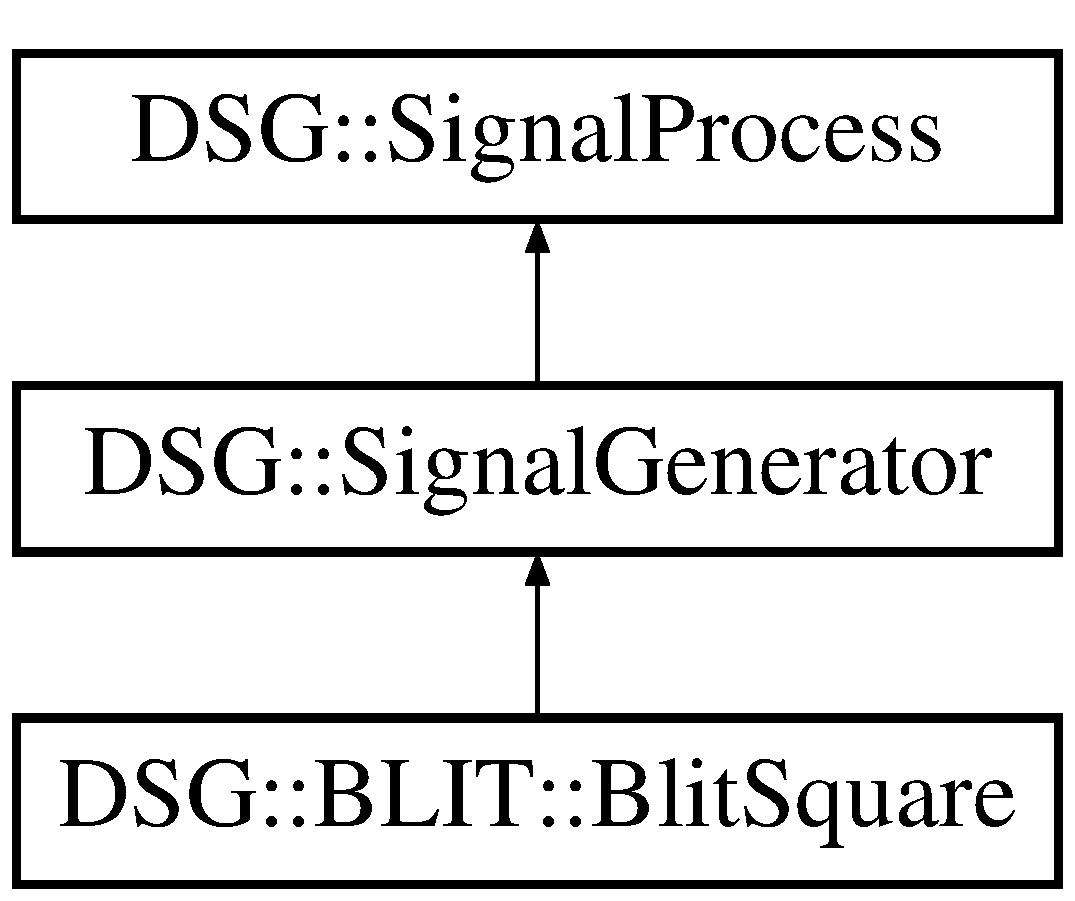
\includegraphics[height=3.000000cm]{class_d_s_g_1_1_b_l_i_t_1_1_blit_square}
\end{center}
\end{figure}
\subsection*{Additional Inherited Members}


\subsection{Detailed Description}
\begin{DoxyRefDesc}{Todo}
\item[\hyperlink{todo__todo000003}{Todo}]Write \hyperlink{class_d_s_g_1_1_b_l_i_t_1_1_blit_square}{D\+S\+G\+::\+B\+L\+I\+T\+::\+Blit\+Square} algorithm \end{DoxyRefDesc}


Definition at line \hyperlink{_b_l_i_t_square_8h_source_l00033}{33} of file \hyperlink{_b_l_i_t_square_8h_source}{B\+L\+I\+T\+Square.\+h}.



The documentation for this class was generated from the following file\+:\begin{DoxyCompactItemize}
\item 
\hyperlink{_b_l_i_t_square_8h}{B\+L\+I\+T\+Square.\+h}\end{DoxyCompactItemize}

\hypertarget{class_d_s_g_1_1_b_l_i_t_1_1_blit_triangle}{\section{D\+S\+G\+:\+:B\+L\+I\+T\+:\+:Blit\+Triangle Class Reference}
\label{class_d_s_g_1_1_b_l_i_t_1_1_blit_triangle}\index{D\+S\+G\+::\+B\+L\+I\+T\+::\+Blit\+Triangle@{D\+S\+G\+::\+B\+L\+I\+T\+::\+Blit\+Triangle}}
}


{\ttfamily \#include $<$B\+L\+I\+T\+Triangle.\+h$>$}

Inheritance diagram for D\+S\+G\+:\+:B\+L\+I\+T\+:\+:Blit\+Triangle\+:\begin{figure}[H]
\begin{center}
\leavevmode
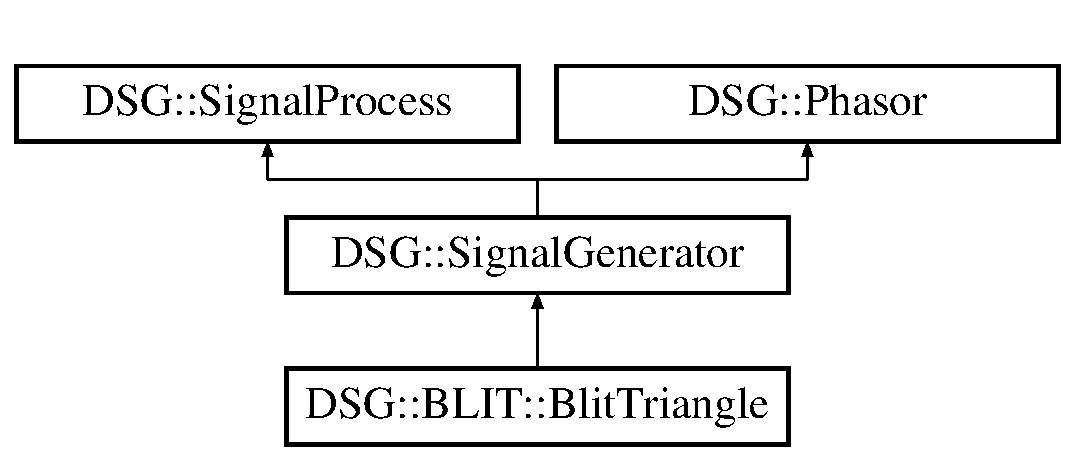
\includegraphics[height=3.000000cm]{class_d_s_g_1_1_b_l_i_t_1_1_blit_triangle}
\end{center}
\end{figure}
\subsection*{Additional Inherited Members}


\subsection{Detailed Description}
\begin{DoxyRefDesc}{Todo}
\item[\hyperlink{todo__todo000004}{Todo}]Write \hyperlink{class_d_s_g_1_1_b_l_i_t_1_1_blit_triangle}{D\+S\+G\+::\+B\+L\+I\+T\+::\+Blit\+Triangle} algorithm \end{DoxyRefDesc}


Definition at line \hyperlink{_b_l_i_t_triangle_8h_source_l00034}{34} of file \hyperlink{_b_l_i_t_triangle_8h_source}{B\+L\+I\+T\+Triangle.\+h}.



The documentation for this class was generated from the following file\+:\begin{DoxyCompactItemize}
\item 
\hyperlink{_b_l_i_t_triangle_8h}{B\+L\+I\+T\+Triangle.\+h}\end{DoxyCompactItemize}

\hypertarget{class_d_s_g_1_1_buffer}{\section{D\+S\+G\+:\+:Buffer Class Reference}
\label{class_d_s_g_1_1_buffer}\index{D\+S\+G\+::\+Buffer@{D\+S\+G\+::\+Buffer}}
}


\hyperlink{class_d_s_g_1_1_buffer}{D\+S\+G\+::\+Buffer} -\/ Base Class For \hyperlink{class_d_s_g_1_1_ring_buffer}{D\+S\+G\+::\+Ring\+Buffer}. Not For Direct Use.  




{\ttfamily \#include $<$Buffer.\+h$>$}

Inheritance diagram for D\+S\+G\+:\+:Buffer\+:\begin{figure}[H]
\begin{center}
\leavevmode
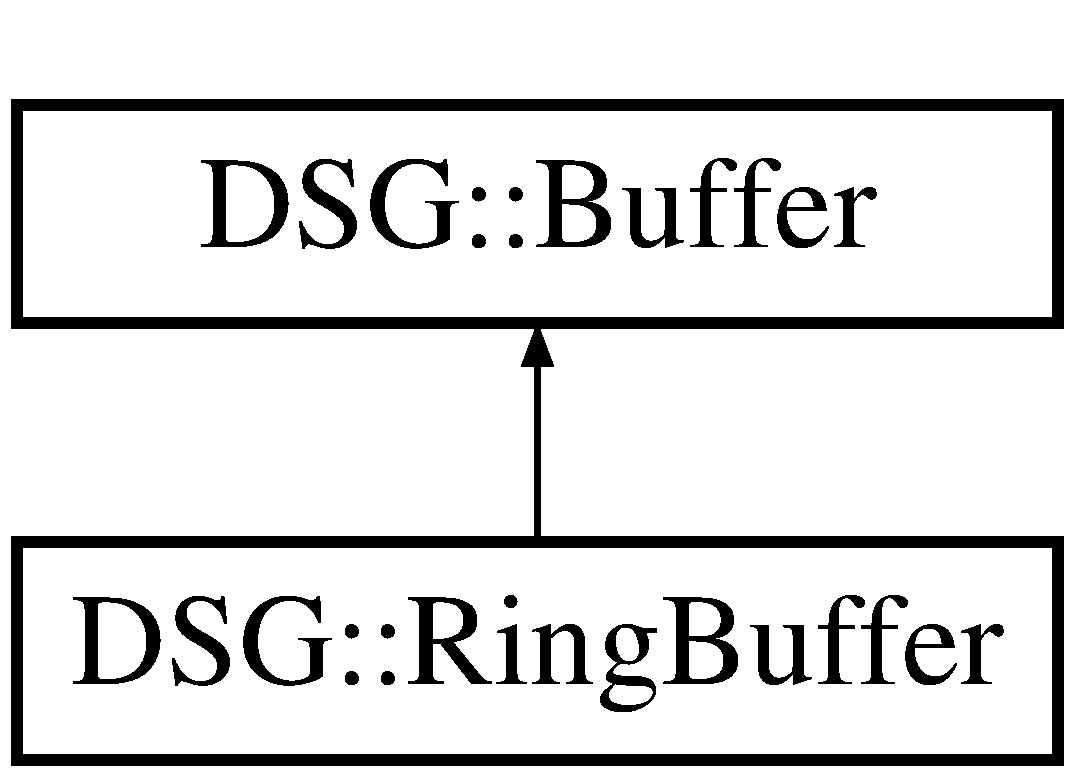
\includegraphics[height=2.000000cm]{class_d_s_g_1_1_buffer}
\end{center}
\end{figure}
\subsection*{Public Member Functions}
\begin{DoxyCompactItemize}
\item 
\hyperlink{class_d_s_g_1_1_buffer_aa764dd8c389dcff51de08cb81fafeb86}{Buffer} ()
\item 
\hyperlink{class_d_s_g_1_1_buffer_a0e6502fd61833043744f9df94e8d5111}{Buffer} (size\+\_\+t size)
\item 
\hyperlink{class_d_s_g_1_1_buffer_a468a65d70553dfb773e4592b4b077683}{Buffer} (\hyperlink{class_d_s_g_1_1_buffer}{Buffer} const \&other)
\item 
\hyperlink{class_d_s_g_1_1_buffer}{Buffer} \& \hyperlink{class_d_s_g_1_1_buffer_a977d572a7d402ff6bf991d7c5c0cc6a7}{operator=} (\hyperlink{class_d_s_g_1_1_buffer}{Buffer} const \&other)
\item 
virtual \hyperlink{class_d_s_g_1_1_buffer_a619fc41bf263a419da1a19254e194101}{$\sim$\+Buffer} ()
\item 
\hyperlink{namespace_d_s_g_ac39a94cd27ebcd9c1e7502d0c624894a}{D\+S\+G\+::\+D\+S\+G\+Sample} \& \hyperlink{class_d_s_g_1_1_buffer_a5358d81096cd0801e4fce7851809b3ef}{operator\mbox{[}$\,$\mbox{]}} (size\+\_\+t const \&index)
\item 
size\+\_\+t const \& \hyperlink{class_d_s_g_1_1_buffer_a4acea659d9cd0be652ec55d21e5b0262}{Size} () const 
\end{DoxyCompactItemize}
\subsection*{Protected Attributes}
\begin{DoxyCompactItemize}
\item 
\hyperlink{namespace_d_s_g_ac39a94cd27ebcd9c1e7502d0c624894a}{D\+S\+G\+::\+D\+S\+G\+Sample} $\ast$ \hyperlink{class_d_s_g_1_1_buffer_ae4a4db8fe44b62db18d6a7855b5773f9}{\+\_\+buffer}
\item 
size\+\_\+t \hyperlink{class_d_s_g_1_1_buffer_a4e2fef9ed617af2554b25c999def8f71}{\+\_\+size}
\end{DoxyCompactItemize}


\subsection{Detailed Description}
\hyperlink{class_d_s_g_1_1_buffer}{D\+S\+G\+::\+Buffer} -\/ Base Class For \hyperlink{class_d_s_g_1_1_ring_buffer}{D\+S\+G\+::\+Ring\+Buffer}. Not For Direct Use. 

Definition at line \hyperlink{_buffer_8h_source_l00018}{18} of file \hyperlink{_buffer_8h_source}{Buffer.\+h}.



\subsection{Constructor \& Destructor Documentation}
\hypertarget{class_d_s_g_1_1_buffer_aa764dd8c389dcff51de08cb81fafeb86}{\index{D\+S\+G\+::\+Buffer@{D\+S\+G\+::\+Buffer}!Buffer@{Buffer}}
\index{Buffer@{Buffer}!D\+S\+G\+::\+Buffer@{D\+S\+G\+::\+Buffer}}
\subsubsection[{Buffer}]{\setlength{\rightskip}{0pt plus 5cm}D\+S\+G\+::\+Buffer\+::\+Buffer (
\begin{DoxyParamCaption}
{}
\end{DoxyParamCaption}
)}}\label{class_d_s_g_1_1_buffer_aa764dd8c389dcff51de08cb81fafeb86}


Definition at line \hyperlink{_buffer_8cpp_source_l00009}{9} of file \hyperlink{_buffer_8cpp_source}{Buffer.\+cpp}.


\begin{DoxyCode}
00009 :\hyperlink{class_d_s_g_1_1_buffer_a4e2fef9ed617af2554b25c999def8f71}{\_size}(0),\hyperlink{class_d_s_g_1_1_buffer_ae4a4db8fe44b62db18d6a7855b5773f9}{\_buffer}(\textcolor{keyword}{nullptr})\{\}
\end{DoxyCode}
\hypertarget{class_d_s_g_1_1_buffer_a0e6502fd61833043744f9df94e8d5111}{\index{D\+S\+G\+::\+Buffer@{D\+S\+G\+::\+Buffer}!Buffer@{Buffer}}
\index{Buffer@{Buffer}!D\+S\+G\+::\+Buffer@{D\+S\+G\+::\+Buffer}}
\subsubsection[{Buffer}]{\setlength{\rightskip}{0pt plus 5cm}D\+S\+G\+::\+Buffer\+::\+Buffer (
\begin{DoxyParamCaption}
\item[{size\+\_\+t}]{size}
\end{DoxyParamCaption}
)}}\label{class_d_s_g_1_1_buffer_a0e6502fd61833043744f9df94e8d5111}


Definition at line \hyperlink{_buffer_8cpp_source_l00010}{10} of file \hyperlink{_buffer_8cpp_source}{Buffer.\+cpp}.


\begin{DoxyCode}
00010 :\hyperlink{class_d_s_g_1_1_buffer_a4e2fef9ed617af2554b25c999def8f71}{\_size}(size),\hyperlink{class_d_s_g_1_1_buffer_ae4a4db8fe44b62db18d6a7855b5773f9}{\_buffer}(\textcolor{keyword}{new} \hyperlink{namespace_d_s_g_ac39a94cd27ebcd9c1e7502d0c624894a}{DSG::DSGSample}[size])\{\}
\end{DoxyCode}
\hypertarget{class_d_s_g_1_1_buffer_a468a65d70553dfb773e4592b4b077683}{\index{D\+S\+G\+::\+Buffer@{D\+S\+G\+::\+Buffer}!Buffer@{Buffer}}
\index{Buffer@{Buffer}!D\+S\+G\+::\+Buffer@{D\+S\+G\+::\+Buffer}}
\subsubsection[{Buffer}]{\setlength{\rightskip}{0pt plus 5cm}D\+S\+G\+::\+Buffer\+::\+Buffer (
\begin{DoxyParamCaption}
\item[{{\bf Buffer} const \&}]{other}
\end{DoxyParamCaption}
)}}\label{class_d_s_g_1_1_buffer_a468a65d70553dfb773e4592b4b077683}


Definition at line \hyperlink{_buffer_8cpp_source_l00011}{11} of file \hyperlink{_buffer_8cpp_source}{Buffer.\+cpp}.


\begin{DoxyCode}
00011                                      \{
00012     \hyperlink{class_d_s_g_1_1_buffer_ae4a4db8fe44b62db18d6a7855b5773f9}{\_buffer} = \textcolor{keyword}{new}  \hyperlink{namespace_d_s_g_ac39a94cd27ebcd9c1e7502d0c624894a}{DSG::DSGSample}[\hyperlink{class_d_s_g_1_1_buffer_a4e2fef9ed617af2554b25c999def8f71}{\_size}];
00013     \hyperlink{class_d_s_g_1_1_buffer_a4e2fef9ed617af2554b25c999def8f71}{\_size} = other.\_size;
00014     *\textcolor{keyword}{this} = other;
00015 \}
\end{DoxyCode}
\hypertarget{class_d_s_g_1_1_buffer_a619fc41bf263a419da1a19254e194101}{\index{D\+S\+G\+::\+Buffer@{D\+S\+G\+::\+Buffer}!````~Buffer@{$\sim$\+Buffer}}
\index{````~Buffer@{$\sim$\+Buffer}!D\+S\+G\+::\+Buffer@{D\+S\+G\+::\+Buffer}}
\subsubsection[{$\sim$\+Buffer}]{\setlength{\rightskip}{0pt plus 5cm}D\+S\+G\+::\+Buffer\+::$\sim$\+Buffer (
\begin{DoxyParamCaption}
{}
\end{DoxyParamCaption}
)\hspace{0.3cm}{\ttfamily [virtual]}}}\label{class_d_s_g_1_1_buffer_a619fc41bf263a419da1a19254e194101}


Definition at line \hyperlink{_buffer_8cpp_source_l00029}{29} of file \hyperlink{_buffer_8cpp_source}{Buffer.\+cpp}.


\begin{DoxyCode}
00029                   \{
00030     \textcolor{keywordflow}{if} (\hyperlink{class_d_s_g_1_1_buffer_ae4a4db8fe44b62db18d6a7855b5773f9}{\_buffer}!=\textcolor{keyword}{nullptr}) \{
00031         \textcolor{keyword}{delete} [] \hyperlink{class_d_s_g_1_1_buffer_ae4a4db8fe44b62db18d6a7855b5773f9}{\_buffer};
00032     \}
00033 \}
\end{DoxyCode}


\subsection{Member Function Documentation}
\hypertarget{class_d_s_g_1_1_buffer_a977d572a7d402ff6bf991d7c5c0cc6a7}{\index{D\+S\+G\+::\+Buffer@{D\+S\+G\+::\+Buffer}!operator=@{operator=}}
\index{operator=@{operator=}!D\+S\+G\+::\+Buffer@{D\+S\+G\+::\+Buffer}}
\subsubsection[{operator=}]{\setlength{\rightskip}{0pt plus 5cm}{\bf D\+S\+G\+::\+Buffer} \& D\+S\+G\+::\+Buffer\+::operator= (
\begin{DoxyParamCaption}
\item[{{\bf Buffer} const \&}]{other}
\end{DoxyParamCaption}
)}}\label{class_d_s_g_1_1_buffer_a977d572a7d402ff6bf991d7c5c0cc6a7}


Definition at line \hyperlink{_buffer_8cpp_source_l00016}{16} of file \hyperlink{_buffer_8cpp_source}{Buffer.\+cpp}.


\begin{DoxyCode}
00016                                                   \{
00017     \textcolor{keywordflow}{if} (\hyperlink{class_d_s_g_1_1_buffer_a4e2fef9ed617af2554b25c999def8f71}{\_size}!=other.\_size) \{
00018         \textcolor{keywordflow}{if} (\hyperlink{class_d_s_g_1_1_buffer_ae4a4db8fe44b62db18d6a7855b5773f9}{\_buffer}!=\textcolor{keyword}{nullptr}) \{
00019             \textcolor{keyword}{delete} [] \hyperlink{class_d_s_g_1_1_buffer_ae4a4db8fe44b62db18d6a7855b5773f9}{\_buffer};
00020         \}
00021         \hyperlink{class_d_s_g_1_1_buffer_a4e2fef9ed617af2554b25c999def8f71}{\_size} = other.\_size;
00022         \hyperlink{class_d_s_g_1_1_buffer_ae4a4db8fe44b62db18d6a7855b5773f9}{\_buffer} = \textcolor{keyword}{new}  \hyperlink{namespace_d_s_g_ac39a94cd27ebcd9c1e7502d0c624894a}{DSG::DSGSample}[\hyperlink{class_d_s_g_1_1_buffer_a4e2fef9ed617af2554b25c999def8f71}{\_size}];
00023     \}
00024     \textcolor{keywordflow}{for} (\textcolor{keywordtype}{int} i=0; i<\hyperlink{class_d_s_g_1_1_buffer_a4e2fef9ed617af2554b25c999def8f71}{\_size}; ++i) \{
00025         \hyperlink{class_d_s_g_1_1_buffer_ae4a4db8fe44b62db18d6a7855b5773f9}{\_buffer}[i] = other.\_buffer[i];
00026     \}
00027     \textcolor{keywordflow}{return} *\textcolor{keyword}{this};
00028 \}
\end{DoxyCode}
\hypertarget{class_d_s_g_1_1_buffer_a5358d81096cd0801e4fce7851809b3ef}{\index{D\+S\+G\+::\+Buffer@{D\+S\+G\+::\+Buffer}!operator\mbox{[}$\,$\mbox{]}@{operator[]}}
\index{operator\mbox{[}$\,$\mbox{]}@{operator[]}!D\+S\+G\+::\+Buffer@{D\+S\+G\+::\+Buffer}}
\subsubsection[{operator[]}]{\setlength{\rightskip}{0pt plus 5cm}{\bf D\+S\+G\+::\+D\+S\+G\+Sample} \& D\+S\+G\+::\+Buffer\+::operator\mbox{[}$\,$\mbox{]} (
\begin{DoxyParamCaption}
\item[{size\+\_\+t const \&}]{index}
\end{DoxyParamCaption}
)}}\label{class_d_s_g_1_1_buffer_a5358d81096cd0801e4fce7851809b3ef}


Definition at line \hyperlink{_buffer_8cpp_source_l00034}{34} of file \hyperlink{_buffer_8cpp_source}{Buffer.\+cpp}.


\begin{DoxyCode}
00034                                                       \{
00035 \textcolor{preprocessor}{#ifdef DEBUG}
00036     assert(index<\hyperlink{class_d_s_g_1_1_buffer_a4e2fef9ed617af2554b25c999def8f71}{\_size});
00037 \textcolor{preprocessor}{#endif}
00038     \textcolor{keywordflow}{return} \hyperlink{class_d_s_g_1_1_buffer_ae4a4db8fe44b62db18d6a7855b5773f9}{\_buffer}[index];
00039 \}\end{DoxyCode}
\hypertarget{class_d_s_g_1_1_buffer_a4acea659d9cd0be652ec55d21e5b0262}{\index{D\+S\+G\+::\+Buffer@{D\+S\+G\+::\+Buffer}!Size@{Size}}
\index{Size@{Size}!D\+S\+G\+::\+Buffer@{D\+S\+G\+::\+Buffer}}
\subsubsection[{Size}]{\setlength{\rightskip}{0pt plus 5cm}size\+\_\+t const \& D\+S\+G\+::\+Buffer\+::\+Size (
\begin{DoxyParamCaption}
{}
\end{DoxyParamCaption}
) const\hspace{0.3cm}{\ttfamily [inline]}}}\label{class_d_s_g_1_1_buffer_a4acea659d9cd0be652ec55d21e5b0262}


Definition at line \hyperlink{_buffer_8h_source_l00031}{31} of file \hyperlink{_buffer_8h_source}{Buffer.\+h}.


\begin{DoxyCode}
00031                                              \{
00032         \textcolor{keywordflow}{return} \hyperlink{class_d_s_g_1_1_buffer_a4e2fef9ed617af2554b25c999def8f71}{\_size};
00033     \}
\end{DoxyCode}


\subsection{Member Data Documentation}
\hypertarget{class_d_s_g_1_1_buffer_ae4a4db8fe44b62db18d6a7855b5773f9}{\index{D\+S\+G\+::\+Buffer@{D\+S\+G\+::\+Buffer}!\+\_\+buffer@{\+\_\+buffer}}
\index{\+\_\+buffer@{\+\_\+buffer}!D\+S\+G\+::\+Buffer@{D\+S\+G\+::\+Buffer}}
\subsubsection[{\+\_\+buffer}]{\setlength{\rightskip}{0pt plus 5cm}{\bf D\+S\+G\+::\+D\+S\+G\+Sample}$\ast$ D\+S\+G\+::\+Buffer\+::\+\_\+buffer\hspace{0.3cm}{\ttfamily [protected]}}}\label{class_d_s_g_1_1_buffer_ae4a4db8fe44b62db18d6a7855b5773f9}


Definition at line \hyperlink{_buffer_8h_source_l00028}{28} of file \hyperlink{_buffer_8h_source}{Buffer.\+h}.

\hypertarget{class_d_s_g_1_1_buffer_a4e2fef9ed617af2554b25c999def8f71}{\index{D\+S\+G\+::\+Buffer@{D\+S\+G\+::\+Buffer}!\+\_\+size@{\+\_\+size}}
\index{\+\_\+size@{\+\_\+size}!D\+S\+G\+::\+Buffer@{D\+S\+G\+::\+Buffer}}
\subsubsection[{\+\_\+size}]{\setlength{\rightskip}{0pt plus 5cm}size\+\_\+t D\+S\+G\+::\+Buffer\+::\+\_\+size\hspace{0.3cm}{\ttfamily [protected]}}}\label{class_d_s_g_1_1_buffer_a4e2fef9ed617af2554b25c999def8f71}


Definition at line \hyperlink{_buffer_8h_source_l00029}{29} of file \hyperlink{_buffer_8h_source}{Buffer.\+h}.



The documentation for this class was generated from the following files\+:\begin{DoxyCompactItemize}
\item 
/\+Users/alexanderzywicki/\+Documents/\+D\+S\+G/src/\hyperlink{_buffer_8h}{Buffer.\+h}\item 
/\+Users/alexanderzywicki/\+Documents/\+D\+S\+G/src/\hyperlink{_buffer_8cpp}{Buffer.\+cpp}\end{DoxyCompactItemize}

\hypertarget{class_d_s_g_1_1_filter_1_1_d_c_blocker}{\section{D\+S\+G\+:\+:Filter\+:\+:D\+C\+Blocker Class Reference}
\label{class_d_s_g_1_1_filter_1_1_d_c_blocker}\index{D\+S\+G\+::\+Filter\+::\+D\+C\+Blocker@{D\+S\+G\+::\+Filter\+::\+D\+C\+Blocker}}
}


\hyperlink{class_d_s_g_1_1_filter_1_1_d_c_blocker}{D\+S\+G\+::\+Filter\+::\+D\+C\+Blocker} -\/ D\+C blocking filter.  




{\ttfamily \#include $<$D\+C\+Blocker.\+h$>$}

Inheritance diagram for D\+S\+G\+:\+:Filter\+:\+:D\+C\+Blocker\+:\begin{figure}[H]
\begin{center}
\leavevmode
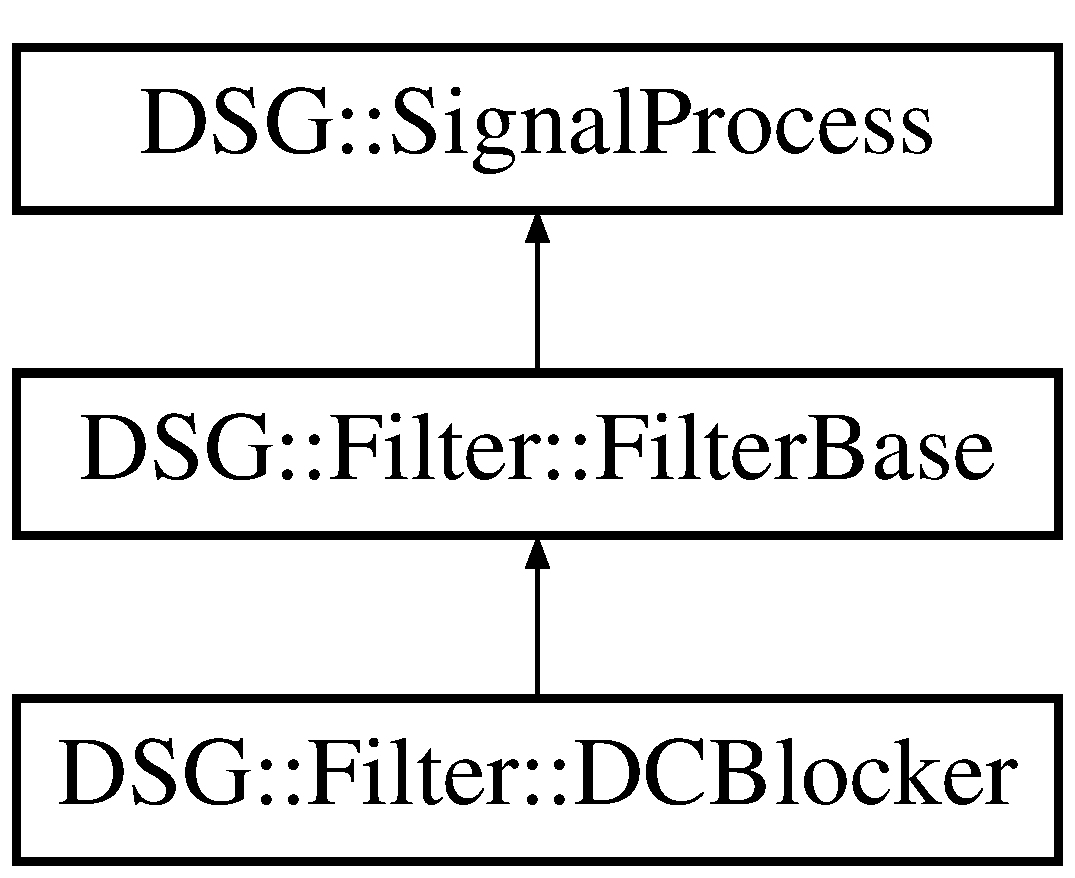
\includegraphics[height=3.000000cm]{class_d_s_g_1_1_filter_1_1_d_c_blocker}
\end{center}
\end{figure}
\subsection*{Public Member Functions}
\begin{DoxyCompactItemize}
\item 
\hyperlink{class_d_s_g_1_1_filter_1_1_d_c_blocker_a71cb7abe6fca10f64402971d8b4a6eb3}{D\+C\+Blocker} ()
\item 
virtual \hyperlink{class_d_s_g_1_1_filter_1_1_d_c_blocker_a5393dac29a226f5912f6d1705b69eecf}{$\sim$\+D\+C\+Blocker} ()
\item 
virtual bool \hyperlink{class_d_s_g_1_1_filter_1_1_d_c_blocker_a9757794b5f9b7789132e5eaa44e07cef}{Perform} (\hyperlink{namespace_d_s_g_ac39a94cd27ebcd9c1e7502d0c624894a}{D\+S\+G\+::\+D\+S\+G\+Sample} \&signal)
\item 
virtual bool \hyperlink{class_d_s_g_1_1_filter_1_1_d_c_blocker_a690b2fdc8fdb749d9832d8d744b8cb2f}{Perform} (\hyperlink{class_d_s_g_1_1_ring_buffer}{D\+S\+G\+::\+Ring\+Buffer} \&signal)
\end{DoxyCompactItemize}
\subsection*{Protected Attributes}
\begin{DoxyCompactItemize}
\item 
unsigned long \hyperlink{class_d_s_g_1_1_filter_1_1_d_c_blocker_a2a045707b5b79e7a4330c87156f7b344}{count}
\item 
\hyperlink{namespace_d_s_g_ac39a94cd27ebcd9c1e7502d0c624894a}{D\+S\+G\+::\+D\+S\+G\+Sample} \hyperlink{class_d_s_g_1_1_filter_1_1_d_c_blocker_a4a698e11be27e8613f5b5146df9c4599}{\+\_\+temp}
\item 
\hyperlink{namespace_d_s_g_ac39a94cd27ebcd9c1e7502d0c624894a}{D\+S\+G\+::\+D\+S\+G\+Sample} \hyperlink{class_d_s_g_1_1_filter_1_1_d_c_blocker_aace7bdafac8d0b4acf9d09bb368f6486}{xm1}
\item 
\hyperlink{namespace_d_s_g_ac39a94cd27ebcd9c1e7502d0c624894a}{D\+S\+G\+::\+D\+S\+G\+Sample} \hyperlink{class_d_s_g_1_1_filter_1_1_d_c_blocker_a61689c80d7fb0f25144fc84996396d71}{ym1}
\item 
\hyperlink{namespace_d_s_g_ac39a94cd27ebcd9c1e7502d0c624894a}{D\+S\+G\+::\+D\+S\+G\+Sample} \hyperlink{class_d_s_g_1_1_filter_1_1_d_c_blocker_aacb82cec9c34b8afe19fe2c7830eb05a}{x}
\item 
\hyperlink{namespace_d_s_g_ac39a94cd27ebcd9c1e7502d0c624894a}{D\+S\+G\+::\+D\+S\+G\+Sample} \hyperlink{class_d_s_g_1_1_filter_1_1_d_c_blocker_ac048fff815764f3ad6d73b27553234c8}{\+\_\+a}
\end{DoxyCompactItemize}


\subsection{Detailed Description}
\hyperlink{class_d_s_g_1_1_filter_1_1_d_c_blocker}{D\+S\+G\+::\+Filter\+::\+D\+C\+Blocker} -\/ D\+C blocking filter. 

Definition at line \hyperlink{_d_c_blocker_8h_source_l00033}{33} of file \hyperlink{_d_c_blocker_8h_source}{D\+C\+Blocker.\+h}.



\subsection{Constructor \& Destructor Documentation}
\hypertarget{class_d_s_g_1_1_filter_1_1_d_c_blocker_a71cb7abe6fca10f64402971d8b4a6eb3}{\index{D\+S\+G\+::\+Filter\+::\+D\+C\+Blocker@{D\+S\+G\+::\+Filter\+::\+D\+C\+Blocker}!D\+C\+Blocker@{D\+C\+Blocker}}
\index{D\+C\+Blocker@{D\+C\+Blocker}!D\+S\+G\+::\+Filter\+::\+D\+C\+Blocker@{D\+S\+G\+::\+Filter\+::\+D\+C\+Blocker}}
\subsubsection[{D\+C\+Blocker}]{\setlength{\rightskip}{0pt plus 5cm}D\+S\+G\+::\+Filter\+::\+D\+C\+Blocker\+::\+D\+C\+Blocker (
\begin{DoxyParamCaption}
{}
\end{DoxyParamCaption}
)}}\label{class_d_s_g_1_1_filter_1_1_d_c_blocker_a71cb7abe6fca10f64402971d8b4a6eb3}


Definition at line \hyperlink{_d_c_blocker_8cpp_source_l00025}{25} of file \hyperlink{_d_c_blocker_8cpp_source}{D\+C\+Blocker.\+cpp}.


\begin{DoxyCode}
00025 :\hyperlink{class_d_s_g_1_1_filter_1_1_filter_base}{DSG::Filter::FilterBase}(),\hyperlink{class_d_s_g_1_1_filter_1_1_d_c_blocker_ac048fff815764f3ad6d73b27553234c8}{\_a}(0.995),\hyperlink{class_d_s_g_1_1_filter_1_1_d_c_blocker_aace7bdafac8d0b4acf9d09bb368f6486}{xm1}(0),\hyperlink{class_d_s_g_1_1_filter_1_1_d_c_blocker_a61689c80d7fb0f25144fc84996396d71}{ym1}(0),
      \hyperlink{class_d_s_g_1_1_filter_1_1_d_c_blocker_aacb82cec9c34b8afe19fe2c7830eb05a}{x}(0),\hyperlink{class_d_s_g_1_1_filter_1_1_d_c_blocker_a4a698e11be27e8613f5b5146df9c4599}{\_temp}(0)\{\}
\end{DoxyCode}
\hypertarget{class_d_s_g_1_1_filter_1_1_d_c_blocker_a5393dac29a226f5912f6d1705b69eecf}{\index{D\+S\+G\+::\+Filter\+::\+D\+C\+Blocker@{D\+S\+G\+::\+Filter\+::\+D\+C\+Blocker}!````~D\+C\+Blocker@{$\sim$\+D\+C\+Blocker}}
\index{````~D\+C\+Blocker@{$\sim$\+D\+C\+Blocker}!D\+S\+G\+::\+Filter\+::\+D\+C\+Blocker@{D\+S\+G\+::\+Filter\+::\+D\+C\+Blocker}}
\subsubsection[{$\sim$\+D\+C\+Blocker}]{\setlength{\rightskip}{0pt plus 5cm}D\+S\+G\+::\+Filter\+::\+D\+C\+Blocker\+::$\sim$\+D\+C\+Blocker (
\begin{DoxyParamCaption}
{}
\end{DoxyParamCaption}
)\hspace{0.3cm}{\ttfamily [virtual]}}}\label{class_d_s_g_1_1_filter_1_1_d_c_blocker_a5393dac29a226f5912f6d1705b69eecf}


Definition at line \hyperlink{_d_c_blocker_8cpp_source_l00026}{26} of file \hyperlink{_d_c_blocker_8cpp_source}{D\+C\+Blocker.\+cpp}.


\begin{DoxyCode}
00026 \{\}\end{DoxyCode}


\subsection{Member Function Documentation}
\hypertarget{class_d_s_g_1_1_filter_1_1_d_c_blocker_a9757794b5f9b7789132e5eaa44e07cef}{\index{D\+S\+G\+::\+Filter\+::\+D\+C\+Blocker@{D\+S\+G\+::\+Filter\+::\+D\+C\+Blocker}!Perform@{Perform}}
\index{Perform@{Perform}!D\+S\+G\+::\+Filter\+::\+D\+C\+Blocker@{D\+S\+G\+::\+Filter\+::\+D\+C\+Blocker}}
\subsubsection[{Perform}]{\setlength{\rightskip}{0pt plus 5cm}bool D\+S\+G\+::\+Filter\+::\+D\+C\+Blocker\+::\+Perform (
\begin{DoxyParamCaption}
\item[{{\bf D\+S\+G\+::\+D\+S\+G\+Sample} \&}]{signal}
\end{DoxyParamCaption}
)\hspace{0.3cm}{\ttfamily [inline]}, {\ttfamily [virtual]}}}\label{class_d_s_g_1_1_filter_1_1_d_c_blocker_a9757794b5f9b7789132e5eaa44e07cef}


Reimplemented from \hyperlink{class_d_s_g_1_1_filter_1_1_filter_base_ae7b6f59f5408ecab3ccd6c4e723c70b4}{D\+S\+G\+::\+Filter\+::\+Filter\+Base}.



Definition at line \hyperlink{_d_c_blocker_8h_source_l00047}{47} of file \hyperlink{_d_c_blocker_8h_source}{D\+C\+Blocker.\+h}.


\begin{DoxyCode}
00047                                                                    \{
00048             \hyperlink{class_d_s_g_1_1_filter_1_1_d_c_blocker_aacb82cec9c34b8afe19fe2c7830eb05a}{x} = signal;
00049             signal= \hyperlink{class_d_s_g_1_1_filter_1_1_d_c_blocker_aacb82cec9c34b8afe19fe2c7830eb05a}{x} - \hyperlink{class_d_s_g_1_1_filter_1_1_d_c_blocker_aace7bdafac8d0b4acf9d09bb368f6486}{xm1}+ (\hyperlink{class_d_s_g_1_1_filter_1_1_d_c_blocker_ac048fff815764f3ad6d73b27553234c8}{\_a} * \hyperlink{class_d_s_g_1_1_filter_1_1_d_c_blocker_a61689c80d7fb0f25144fc84996396d71}{ym1});
00050             \hyperlink{class_d_s_g_1_1_filter_1_1_d_c_blocker_aace7bdafac8d0b4acf9d09bb368f6486}{xm1} = \hyperlink{class_d_s_g_1_1_filter_1_1_d_c_blocker_aacb82cec9c34b8afe19fe2c7830eb05a}{x};
00051             \hyperlink{class_d_s_g_1_1_filter_1_1_d_c_blocker_a61689c80d7fb0f25144fc84996396d71}{ym1}=signal;
00052             \textcolor{keywordflow}{return} \textcolor{keyword}{true};
00053         \}
\end{DoxyCode}
\hypertarget{class_d_s_g_1_1_filter_1_1_d_c_blocker_a690b2fdc8fdb749d9832d8d744b8cb2f}{\index{D\+S\+G\+::\+Filter\+::\+D\+C\+Blocker@{D\+S\+G\+::\+Filter\+::\+D\+C\+Blocker}!Perform@{Perform}}
\index{Perform@{Perform}!D\+S\+G\+::\+Filter\+::\+D\+C\+Blocker@{D\+S\+G\+::\+Filter\+::\+D\+C\+Blocker}}
\subsubsection[{Perform}]{\setlength{\rightskip}{0pt plus 5cm}bool D\+S\+G\+::\+Filter\+::\+D\+C\+Blocker\+::\+Perform (
\begin{DoxyParamCaption}
\item[{{\bf D\+S\+G\+::\+Ring\+Buffer} \&}]{signal}
\end{DoxyParamCaption}
)\hspace{0.3cm}{\ttfamily [inline]}, {\ttfamily [virtual]}}}\label{class_d_s_g_1_1_filter_1_1_d_c_blocker_a690b2fdc8fdb749d9832d8d744b8cb2f}


Reimplemented from \hyperlink{class_d_s_g_1_1_filter_1_1_filter_base_aef58742a1362b7ef94574a16036b7109}{D\+S\+G\+::\+Filter\+::\+Filter\+Base}.



Definition at line \hyperlink{_d_c_blocker_8h_source_l00054}{54} of file \hyperlink{_d_c_blocker_8h_source}{D\+C\+Blocker.\+h}.


\begin{DoxyCode}
00054                                                                     \{
00055             \textcolor{keywordflow}{if} (!signal.\hyperlink{class_d_s_g_1_1_ring_buffer_ac1346f5842d08b988a5297abe4089b96}{Empty}()) \{
00056                 \hyperlink{class_d_s_g_1_1_filter_1_1_d_c_blocker_a2a045707b5b79e7a4330c87156f7b344}{count} = signal.\hyperlink{class_d_s_g_1_1_ring_buffer_a9bd79b0a6dff618b205e396c101ee070}{Count}();
00057                 \textcolor{keywordflow}{while} (\hyperlink{class_d_s_g_1_1_filter_1_1_d_c_blocker_a2a045707b5b79e7a4330c87156f7b344}{count}-- > 0) \{
00058                     \textcolor{keywordflow}{if}(signal.\hyperlink{class_d_s_g_1_1_ring_buffer_a6b2848a64f15c7b0c320779582fa0fbe}{Read}(\hyperlink{class_d_s_g_1_1_filter_1_1_d_c_blocker_a4a698e11be27e8613f5b5146df9c4599}{\_temp}))\{
00059                         \textcolor{keywordflow}{if} (\hyperlink{class_d_s_g_1_1_filter_1_1_d_c_blocker_a9757794b5f9b7789132e5eaa44e07cef}{Perform}(\hyperlink{class_d_s_g_1_1_filter_1_1_d_c_blocker_a4a698e11be27e8613f5b5146df9c4599}{\_temp})) \{
00060                             signal.\hyperlink{class_d_s_g_1_1_ring_buffer_aa5dd2caa0a270173251faee40a43d692}{Write}(\hyperlink{class_d_s_g_1_1_filter_1_1_d_c_blocker_a4a698e11be27e8613f5b5146df9c4599}{\_temp});
00061                         \}\textcolor{keywordflow}{else} \textcolor{keywordflow}{return} \textcolor{keyword}{false};
00062                     \}\textcolor{keywordflow}{else} \textcolor{keywordflow}{return} \textcolor{keyword}{false};
00063                 \}\textcolor{keywordflow}{return} \textcolor{keyword}{true};
00064             \}\textcolor{keywordflow}{else} \textcolor{keywordflow}{return} \textcolor{keyword}{false};
00065         \}
\end{DoxyCode}


\subsection{Member Data Documentation}
\hypertarget{class_d_s_g_1_1_filter_1_1_d_c_blocker_ac048fff815764f3ad6d73b27553234c8}{\index{D\+S\+G\+::\+Filter\+::\+D\+C\+Blocker@{D\+S\+G\+::\+Filter\+::\+D\+C\+Blocker}!\+\_\+a@{\+\_\+a}}
\index{\+\_\+a@{\+\_\+a}!D\+S\+G\+::\+Filter\+::\+D\+C\+Blocker@{D\+S\+G\+::\+Filter\+::\+D\+C\+Blocker}}
\subsubsection[{\+\_\+a}]{\setlength{\rightskip}{0pt plus 5cm}{\bf D\+S\+G\+::\+D\+S\+G\+Sample} D\+S\+G\+::\+Filter\+::\+D\+C\+Blocker\+::\+\_\+a\hspace{0.3cm}{\ttfamily [protected]}}}\label{class_d_s_g_1_1_filter_1_1_d_c_blocker_ac048fff815764f3ad6d73b27553234c8}


Definition at line \hyperlink{_d_c_blocker_8h_source_l00045}{45} of file \hyperlink{_d_c_blocker_8h_source}{D\+C\+Blocker.\+h}.

\hypertarget{class_d_s_g_1_1_filter_1_1_d_c_blocker_a4a698e11be27e8613f5b5146df9c4599}{\index{D\+S\+G\+::\+Filter\+::\+D\+C\+Blocker@{D\+S\+G\+::\+Filter\+::\+D\+C\+Blocker}!\+\_\+temp@{\+\_\+temp}}
\index{\+\_\+temp@{\+\_\+temp}!D\+S\+G\+::\+Filter\+::\+D\+C\+Blocker@{D\+S\+G\+::\+Filter\+::\+D\+C\+Blocker}}
\subsubsection[{\+\_\+temp}]{\setlength{\rightskip}{0pt plus 5cm}{\bf D\+S\+G\+::\+D\+S\+G\+Sample} D\+S\+G\+::\+Filter\+::\+D\+C\+Blocker\+::\+\_\+temp\hspace{0.3cm}{\ttfamily [protected]}}}\label{class_d_s_g_1_1_filter_1_1_d_c_blocker_a4a698e11be27e8613f5b5146df9c4599}


Definition at line \hyperlink{_d_c_blocker_8h_source_l00041}{41} of file \hyperlink{_d_c_blocker_8h_source}{D\+C\+Blocker.\+h}.

\hypertarget{class_d_s_g_1_1_filter_1_1_d_c_blocker_a2a045707b5b79e7a4330c87156f7b344}{\index{D\+S\+G\+::\+Filter\+::\+D\+C\+Blocker@{D\+S\+G\+::\+Filter\+::\+D\+C\+Blocker}!count@{count}}
\index{count@{count}!D\+S\+G\+::\+Filter\+::\+D\+C\+Blocker@{D\+S\+G\+::\+Filter\+::\+D\+C\+Blocker}}
\subsubsection[{count}]{\setlength{\rightskip}{0pt plus 5cm}unsigned long D\+S\+G\+::\+Filter\+::\+D\+C\+Blocker\+::count\hspace{0.3cm}{\ttfamily [protected]}}}\label{class_d_s_g_1_1_filter_1_1_d_c_blocker_a2a045707b5b79e7a4330c87156f7b344}


Definition at line \hyperlink{_d_c_blocker_8h_source_l00040}{40} of file \hyperlink{_d_c_blocker_8h_source}{D\+C\+Blocker.\+h}.

\hypertarget{class_d_s_g_1_1_filter_1_1_d_c_blocker_aacb82cec9c34b8afe19fe2c7830eb05a}{\index{D\+S\+G\+::\+Filter\+::\+D\+C\+Blocker@{D\+S\+G\+::\+Filter\+::\+D\+C\+Blocker}!x@{x}}
\index{x@{x}!D\+S\+G\+::\+Filter\+::\+D\+C\+Blocker@{D\+S\+G\+::\+Filter\+::\+D\+C\+Blocker}}
\subsubsection[{x}]{\setlength{\rightskip}{0pt plus 5cm}{\bf D\+S\+G\+::\+D\+S\+G\+Sample} D\+S\+G\+::\+Filter\+::\+D\+C\+Blocker\+::x\hspace{0.3cm}{\ttfamily [protected]}}}\label{class_d_s_g_1_1_filter_1_1_d_c_blocker_aacb82cec9c34b8afe19fe2c7830eb05a}


Definition at line \hyperlink{_d_c_blocker_8h_source_l00044}{44} of file \hyperlink{_d_c_blocker_8h_source}{D\+C\+Blocker.\+h}.

\hypertarget{class_d_s_g_1_1_filter_1_1_d_c_blocker_aace7bdafac8d0b4acf9d09bb368f6486}{\index{D\+S\+G\+::\+Filter\+::\+D\+C\+Blocker@{D\+S\+G\+::\+Filter\+::\+D\+C\+Blocker}!xm1@{xm1}}
\index{xm1@{xm1}!D\+S\+G\+::\+Filter\+::\+D\+C\+Blocker@{D\+S\+G\+::\+Filter\+::\+D\+C\+Blocker}}
\subsubsection[{xm1}]{\setlength{\rightskip}{0pt plus 5cm}{\bf D\+S\+G\+::\+D\+S\+G\+Sample} D\+S\+G\+::\+Filter\+::\+D\+C\+Blocker\+::xm1\hspace{0.3cm}{\ttfamily [protected]}}}\label{class_d_s_g_1_1_filter_1_1_d_c_blocker_aace7bdafac8d0b4acf9d09bb368f6486}


Definition at line \hyperlink{_d_c_blocker_8h_source_l00042}{42} of file \hyperlink{_d_c_blocker_8h_source}{D\+C\+Blocker.\+h}.

\hypertarget{class_d_s_g_1_1_filter_1_1_d_c_blocker_a61689c80d7fb0f25144fc84996396d71}{\index{D\+S\+G\+::\+Filter\+::\+D\+C\+Blocker@{D\+S\+G\+::\+Filter\+::\+D\+C\+Blocker}!ym1@{ym1}}
\index{ym1@{ym1}!D\+S\+G\+::\+Filter\+::\+D\+C\+Blocker@{D\+S\+G\+::\+Filter\+::\+D\+C\+Blocker}}
\subsubsection[{ym1}]{\setlength{\rightskip}{0pt plus 5cm}{\bf D\+S\+G\+::\+D\+S\+G\+Sample} D\+S\+G\+::\+Filter\+::\+D\+C\+Blocker\+::ym1\hspace{0.3cm}{\ttfamily [protected]}}}\label{class_d_s_g_1_1_filter_1_1_d_c_blocker_a61689c80d7fb0f25144fc84996396d71}


Definition at line \hyperlink{_d_c_blocker_8h_source_l00043}{43} of file \hyperlink{_d_c_blocker_8h_source}{D\+C\+Blocker.\+h}.



The documentation for this class was generated from the following files\+:\begin{DoxyCompactItemize}
\item 
\hyperlink{_d_c_blocker_8h}{D\+C\+Blocker.\+h}\item 
\hyperlink{_d_c_blocker_8cpp}{D\+C\+Blocker.\+cpp}\end{DoxyCompactItemize}

\hypertarget{class_d_s_g_1_1_delay}{\section{D\+S\+G\+:\+:Delay$<$ max\+Length $>$ Class Template Reference}
\label{class_d_s_g_1_1_delay}\index{D\+S\+G\+::\+Delay$<$ max\+Length $>$@{D\+S\+G\+::\+Delay$<$ max\+Length $>$}}
}


\hyperlink{class_d_s_g_1_1_delay}{D\+S\+G\+::\+Delay} -\/ General purpose delay line.  




{\ttfamily \#include $<$Delay.\+h$>$}

Inheritance diagram for D\+S\+G\+:\+:Delay$<$ max\+Length $>$\+:\begin{figure}[H]
\begin{center}
\leavevmode
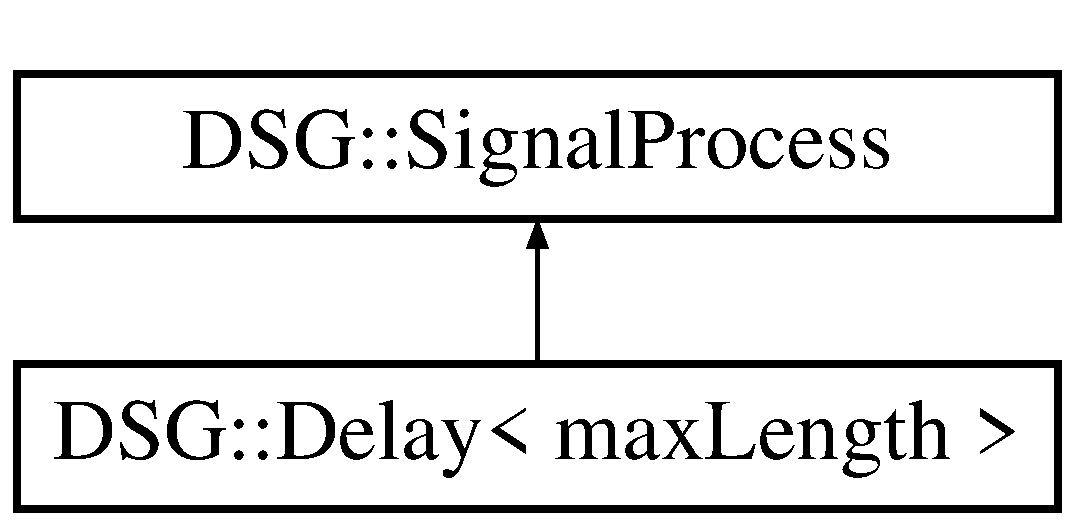
\includegraphics[height=2.000000cm]{class_d_s_g_1_1_delay}
\end{center}
\end{figure}
\subsection*{Public Member Functions}
\begin{DoxyCompactItemize}
\item 
\hyperlink{class_d_s_g_1_1_delay_a20fb108695dac24156aeb2143a88555a}{Delay} ()
\item 
\hyperlink{class_d_s_g_1_1_delay_aecfa312690df905bbeaa8888d1bb702f}{Delay} (double const \&samples)
\item 
virtual \hyperlink{class_d_s_g_1_1_delay_ac2df9a0120744cc8efa15556e4293a2c}{$\sim$\+Delay} ()
\item 
virtual unsigned long const \& \hyperlink{class_d_s_g_1_1_delay_abf8bfbd184f1e733d1b5aae0bfa408d7}{Length} () const 
\item 
virtual unsigned long const \& \hyperlink{class_d_s_g_1_1_delay_a7081f684727044ff1765ab6284385359}{Length} (unsigned long const \&samples)
\item 
virtual bool \hyperlink{class_d_s_g_1_1_delay_afe853b73a1d7d1e5720277e5d956b209}{Perform} (\hyperlink{namespace_d_s_g_ac39a94cd27ebcd9c1e7502d0c624894a}{D\+S\+G\+::\+D\+S\+G\+Sample} \&signal)
\item 
virtual bool \hyperlink{class_d_s_g_1_1_delay_a205bd6fc25ea951395943eae51128e66}{Perform} (\hyperlink{class_d_s_g_1_1_ring_buffer}{D\+S\+G\+::\+Ring\+Buffer} \&signal)
\end{DoxyCompactItemize}
\subsection*{Protected Member Functions}
\begin{DoxyCompactItemize}
\item 
virtual void \hyperlink{class_d_s_g_1_1_delay_a4c800f6ce87a75d964aab53617d12664}{increment} ()
\end{DoxyCompactItemize}
\subsection*{Protected Attributes}
\begin{DoxyCompactItemize}
\item 
unsigned long \hyperlink{class_d_s_g_1_1_delay_a1d54836950db9724434880d859d1e3ea}{count}
\item 
unsigned long \hyperlink{class_d_s_g_1_1_delay_aad8790118689ae46c7f434b790358e3f}{\+\_\+delay}
\item 
unsigned long \hyperlink{class_d_s_g_1_1_delay_ac39e72226786a3c43b231b69752431ec}{\+\_\+index}
\item 
const unsigned long \hyperlink{class_d_s_g_1_1_delay_a1751998677ff85f6580c383e17347d9c}{\+\_\+max}
\item 
\hyperlink{namespace_d_s_g_ac39a94cd27ebcd9c1e7502d0c624894a}{D\+S\+G\+::\+D\+S\+G\+Sample} \hyperlink{class_d_s_g_1_1_delay_a8c86e03e9656476371f98d049ae1c5c9}{\+\_\+buffer} \mbox{[}max\+Length\mbox{]}
\item 
\hyperlink{namespace_d_s_g_ac39a94cd27ebcd9c1e7502d0c624894a}{D\+S\+G\+::\+D\+S\+G\+Sample} \hyperlink{class_d_s_g_1_1_delay_af026ee90120c5cea6a935aef6cab6624}{\+\_\+swap}
\item 
\hyperlink{namespace_d_s_g_ac39a94cd27ebcd9c1e7502d0c624894a}{D\+S\+G\+::\+D\+S\+G\+Sample} \hyperlink{class_d_s_g_1_1_delay_a039bb7a3a39aff5841b9e808cacc1a6e}{\+\_\+temp}
\end{DoxyCompactItemize}


\subsection{Detailed Description}
\subsubsection*{template$<$unsigned long max\+Length$>$class D\+S\+G\+::\+Delay$<$ max\+Length $>$}

\hyperlink{class_d_s_g_1_1_delay}{D\+S\+G\+::\+Delay} -\/ General purpose delay line. 

Definition at line \hyperlink{_delay_8h_source_l00017}{17} of file \hyperlink{_delay_8h_source}{Delay.\+h}.



\subsection{Constructor \& Destructor Documentation}
\hypertarget{class_d_s_g_1_1_delay_a20fb108695dac24156aeb2143a88555a}{\index{D\+S\+G\+::\+Delay@{D\+S\+G\+::\+Delay}!Delay@{Delay}}
\index{Delay@{Delay}!D\+S\+G\+::\+Delay@{D\+S\+G\+::\+Delay}}
\subsubsection[{Delay}]{\setlength{\rightskip}{0pt plus 5cm}template$<$unsigned long max\+Length$>$ {\bf D\+S\+G\+::\+Delay}$<$ max\+Length $>$\+::{\bf Delay} (
\begin{DoxyParamCaption}
{}
\end{DoxyParamCaption}
)\hspace{0.3cm}{\ttfamily [inline]}}}\label{class_d_s_g_1_1_delay_a20fb108695dac24156aeb2143a88555a}


Definition at line \hyperlink{_delay_8h_source_l00019}{19} of file \hyperlink{_delay_8h_source}{Delay.\+h}.


\begin{DoxyCode}
00019                :\hyperlink{class_d_s_g_1_1_signal_process}{DSG::SignalProcess}(),\hyperlink{class_d_s_g_1_1_delay_a1751998677ff85f6580c383e17347d9c}{\_max}(maxLength),\hyperlink{class_d_s_g_1_1_delay_af026ee90120c5cea6a935aef6cab6624}{\_swap}(0),
      \hyperlink{class_d_s_g_1_1_delay_a039bb7a3a39aff5841b9e808cacc1a6e}{\_temp}(0),\hyperlink{class_d_s_g_1_1_delay_a1d54836950db9724434880d859d1e3ea}{count}(0),\hyperlink{class_d_s_g_1_1_delay_ac39e72226786a3c43b231b69752431ec}{\_index}(0),\hyperlink{class_d_s_g_1_1_delay_aad8790118689ae46c7f434b790358e3f}{\_delay}(0)\{
00020             \textcolor{keywordflow}{for} (\textcolor{keywordtype}{int} i=0; i<\hyperlink{class_d_s_g_1_1_delay_a1751998677ff85f6580c383e17347d9c}{\_max}; ++i) \{
00021                 \hyperlink{class_d_s_g_1_1_delay_a8c86e03e9656476371f98d049ae1c5c9}{\_buffer}[i]=0;
00022             \}
00023         \}
\end{DoxyCode}
\hypertarget{class_d_s_g_1_1_delay_aecfa312690df905bbeaa8888d1bb702f}{\index{D\+S\+G\+::\+Delay@{D\+S\+G\+::\+Delay}!Delay@{Delay}}
\index{Delay@{Delay}!D\+S\+G\+::\+Delay@{D\+S\+G\+::\+Delay}}
\subsubsection[{Delay}]{\setlength{\rightskip}{0pt plus 5cm}template$<$unsigned long max\+Length$>$ {\bf D\+S\+G\+::\+Delay}$<$ max\+Length $>$\+::{\bf Delay} (
\begin{DoxyParamCaption}
\item[{double const \&}]{samples}
\end{DoxyParamCaption}
)\hspace{0.3cm}{\ttfamily [inline]}}}\label{class_d_s_g_1_1_delay_aecfa312690df905bbeaa8888d1bb702f}


Definition at line \hyperlink{_delay_8h_source_l00024}{24} of file \hyperlink{_delay_8h_source}{Delay.\+h}.


\begin{DoxyCode}
00024                                     :\hyperlink{class_d_s_g_1_1_signal_process}{DSG::SignalProcess}(),\hyperlink{class_d_s_g_1_1_delay_a1751998677ff85f6580c383e17347d9c}{\_max}(maxLength),
      \hyperlink{class_d_s_g_1_1_delay_af026ee90120c5cea6a935aef6cab6624}{\_swap}(0),\hyperlink{class_d_s_g_1_1_delay_a039bb7a3a39aff5841b9e808cacc1a6e}{\_temp}(0),\hyperlink{class_d_s_g_1_1_delay_a1d54836950db9724434880d859d1e3ea}{count}(0),\hyperlink{class_d_s_g_1_1_delay_ac39e72226786a3c43b231b69752431ec}{\_index}(0),\hyperlink{class_d_s_g_1_1_delay_aad8790118689ae46c7f434b790358e3f}{\_delay}(0)\{
00025             \textcolor{keywordflow}{for} (\textcolor{keywordtype}{int} i=0; i<\hyperlink{class_d_s_g_1_1_delay_a1751998677ff85f6580c383e17347d9c}{\_max}; ++i) \{
00026                 \hyperlink{class_d_s_g_1_1_delay_a8c86e03e9656476371f98d049ae1c5c9}{\_buffer}[i]=0;
00027             \}
00028             \textcolor{keywordflow}{if} (samples>maxLength) \{
00029                 \hyperlink{class_d_s_g_1_1_delay_aad8790118689ae46c7f434b790358e3f}{\_delay} = maxLength;
00030             \}\textcolor{keywordflow}{else}\{
00031                 \hyperlink{class_d_s_g_1_1_delay_aad8790118689ae46c7f434b790358e3f}{\_delay} = samples;
00032             \}
00033         \}
\end{DoxyCode}
\hypertarget{class_d_s_g_1_1_delay_ac2df9a0120744cc8efa15556e4293a2c}{\index{D\+S\+G\+::\+Delay@{D\+S\+G\+::\+Delay}!````~Delay@{$\sim$\+Delay}}
\index{````~Delay@{$\sim$\+Delay}!D\+S\+G\+::\+Delay@{D\+S\+G\+::\+Delay}}
\subsubsection[{$\sim$\+Delay}]{\setlength{\rightskip}{0pt plus 5cm}template$<$unsigned long max\+Length$>$ virtual {\bf D\+S\+G\+::\+Delay}$<$ max\+Length $>$\+::$\sim${\bf Delay} (
\begin{DoxyParamCaption}
{}
\end{DoxyParamCaption}
)\hspace{0.3cm}{\ttfamily [inline]}, {\ttfamily [virtual]}}}\label{class_d_s_g_1_1_delay_ac2df9a0120744cc8efa15556e4293a2c}


Definition at line \hyperlink{_delay_8h_source_l00034}{34} of file \hyperlink{_delay_8h_source}{Delay.\+h}.


\begin{DoxyCode}
00034 \{\}
\end{DoxyCode}


\subsection{Member Function Documentation}
\hypertarget{class_d_s_g_1_1_delay_a4c800f6ce87a75d964aab53617d12664}{\index{D\+S\+G\+::\+Delay@{D\+S\+G\+::\+Delay}!increment@{increment}}
\index{increment@{increment}!D\+S\+G\+::\+Delay@{D\+S\+G\+::\+Delay}}
\subsubsection[{increment}]{\setlength{\rightskip}{0pt plus 5cm}template$<$unsigned long max\+Length$>$ virtual void {\bf D\+S\+G\+::\+Delay}$<$ max\+Length $>$\+::increment (
\begin{DoxyParamCaption}
{}
\end{DoxyParamCaption}
)\hspace{0.3cm}{\ttfamily [inline]}, {\ttfamily [protected]}, {\ttfamily [virtual]}}}\label{class_d_s_g_1_1_delay_a4c800f6ce87a75d964aab53617d12664}


Definition at line \hyperlink{_delay_8h_source_l00056}{56} of file \hyperlink{_delay_8h_source}{Delay.\+h}.


\begin{DoxyCode}
00056                                        \{
00057             ++\hyperlink{class_d_s_g_1_1_delay_ac39e72226786a3c43b231b69752431ec}{\_index};
00058             \textcolor{keywordflow}{if} (\hyperlink{class_d_s_g_1_1_delay_ac39e72226786a3c43b231b69752431ec}{\_index}>\hyperlink{class_d_s_g_1_1_delay_aad8790118689ae46c7f434b790358e3f}{\_delay}) \{
00059                 \hyperlink{class_d_s_g_1_1_delay_ac39e72226786a3c43b231b69752431ec}{\_index}-=\hyperlink{class_d_s_g_1_1_delay_aad8790118689ae46c7f434b790358e3f}{\_delay};
00060             \}
00061         \}
\end{DoxyCode}
\hypertarget{class_d_s_g_1_1_delay_abf8bfbd184f1e733d1b5aae0bfa408d7}{\index{D\+S\+G\+::\+Delay@{D\+S\+G\+::\+Delay}!Length@{Length}}
\index{Length@{Length}!D\+S\+G\+::\+Delay@{D\+S\+G\+::\+Delay}}
\subsubsection[{Length}]{\setlength{\rightskip}{0pt plus 5cm}template$<$unsigned long max\+Length$>$ virtual unsigned long const\& {\bf D\+S\+G\+::\+Delay}$<$ max\+Length $>$\+::Length (
\begin{DoxyParamCaption}
{}
\end{DoxyParamCaption}
) const\hspace{0.3cm}{\ttfamily [inline]}, {\ttfamily [virtual]}}}\label{class_d_s_g_1_1_delay_abf8bfbd184f1e733d1b5aae0bfa408d7}


Definition at line \hyperlink{_delay_8h_source_l00035}{35} of file \hyperlink{_delay_8h_source}{Delay.\+h}.


\begin{DoxyCode}
00035                                                          \{
00036             \textcolor{keywordflow}{return} \hyperlink{class_d_s_g_1_1_delay_aad8790118689ae46c7f434b790358e3f}{\_delay};
00037         \}
\end{DoxyCode}
\hypertarget{class_d_s_g_1_1_delay_a7081f684727044ff1765ab6284385359}{\index{D\+S\+G\+::\+Delay@{D\+S\+G\+::\+Delay}!Length@{Length}}
\index{Length@{Length}!D\+S\+G\+::\+Delay@{D\+S\+G\+::\+Delay}}
\subsubsection[{Length}]{\setlength{\rightskip}{0pt plus 5cm}template$<$unsigned long max\+Length$>$ virtual unsigned long const\& {\bf D\+S\+G\+::\+Delay}$<$ max\+Length $>$\+::Length (
\begin{DoxyParamCaption}
\item[{unsigned long const \&}]{samples}
\end{DoxyParamCaption}
)\hspace{0.3cm}{\ttfamily [inline]}, {\ttfamily [virtual]}}}\label{class_d_s_g_1_1_delay_a7081f684727044ff1765ab6284385359}


Definition at line \hyperlink{_delay_8h_source_l00038}{38} of file \hyperlink{_delay_8h_source}{Delay.\+h}.


\begin{DoxyCode}
00038                                                                                 \{
00039             \textcolor{keywordflow}{if} (samples>maxLength) \{
00040                 \hyperlink{class_d_s_g_1_1_delay_aad8790118689ae46c7f434b790358e3f}{\_delay} = maxLength;
00041             \}\textcolor{keywordflow}{else}\{
00042                 \hyperlink{class_d_s_g_1_1_delay_aad8790118689ae46c7f434b790358e3f}{\_delay} = samples;
00043             \}
00044             \textcolor{keywordflow}{return} \hyperlink{class_d_s_g_1_1_delay_aad8790118689ae46c7f434b790358e3f}{\_delay};
00045         \}
\end{DoxyCode}
\hypertarget{class_d_s_g_1_1_delay_afe853b73a1d7d1e5720277e5d956b209}{\index{D\+S\+G\+::\+Delay@{D\+S\+G\+::\+Delay}!Perform@{Perform}}
\index{Perform@{Perform}!D\+S\+G\+::\+Delay@{D\+S\+G\+::\+Delay}}
\subsubsection[{Perform}]{\setlength{\rightskip}{0pt plus 5cm}template$<$unsigned long max\+Length$>$ bool {\bf D\+S\+G\+::\+Delay}$<$ max\+Length $>$\+::Perform (
\begin{DoxyParamCaption}
\item[{{\bf D\+S\+G\+::\+D\+S\+G\+Sample} \&}]{signal}
\end{DoxyParamCaption}
)\hspace{0.3cm}{\ttfamily [inline]}, {\ttfamily [virtual]}}}\label{class_d_s_g_1_1_delay_afe853b73a1d7d1e5720277e5d956b209}


Implements \hyperlink{class_d_s_g_1_1_signal_process_af73d246c460915db7a9be7e3ef36844d}{D\+S\+G\+::\+Signal\+Process}.



Definition at line \hyperlink{_delay_8h_source_l00064}{64} of file \hyperlink{_delay_8h_source}{Delay.\+h}.


\begin{DoxyCode}
00064                                                                 \{
00065         \hyperlink{class_d_s_g_1_1_delay_af026ee90120c5cea6a935aef6cab6624}{\_swap} = \hyperlink{class_d_s_g_1_1_delay_a8c86e03e9656476371f98d049ae1c5c9}{\_buffer}[\hyperlink{class_d_s_g_1_1_delay_ac39e72226786a3c43b231b69752431ec}{\_index}-1];
00066         \hyperlink{class_d_s_g_1_1_delay_a8c86e03e9656476371f98d049ae1c5c9}{\_buffer}[\hyperlink{class_d_s_g_1_1_delay_ac39e72226786a3c43b231b69752431ec}{\_index}-1]=signal;
00067         signal = \hyperlink{class_d_s_g_1_1_delay_af026ee90120c5cea6a935aef6cab6624}{\_swap};
00068         \hyperlink{class_d_s_g_1_1_delay_a4c800f6ce87a75d964aab53617d12664}{increment}();
00069         \textcolor{keywordflow}{return} \textcolor{keyword}{true};
00070     \}
\end{DoxyCode}
\hypertarget{class_d_s_g_1_1_delay_a205bd6fc25ea951395943eae51128e66}{\index{D\+S\+G\+::\+Delay@{D\+S\+G\+::\+Delay}!Perform@{Perform}}
\index{Perform@{Perform}!D\+S\+G\+::\+Delay@{D\+S\+G\+::\+Delay}}
\subsubsection[{Perform}]{\setlength{\rightskip}{0pt plus 5cm}template$<$unsigned long max\+Length$>$ bool {\bf D\+S\+G\+::\+Delay}$<$ max\+Length $>$\+::Perform (
\begin{DoxyParamCaption}
\item[{{\bf D\+S\+G\+::\+Ring\+Buffer} \&}]{signal}
\end{DoxyParamCaption}
)\hspace{0.3cm}{\ttfamily [inline]}, {\ttfamily [virtual]}}}\label{class_d_s_g_1_1_delay_a205bd6fc25ea951395943eae51128e66}


Implements \hyperlink{class_d_s_g_1_1_signal_process_a2c8ff3487d9c43f9eace1d9192d4a37e}{D\+S\+G\+::\+Signal\+Process}.



Definition at line \hyperlink{_delay_8h_source_l00072}{72} of file \hyperlink{_delay_8h_source}{Delay.\+h}.


\begin{DoxyCode}
00072                                                                  \{
00073         \textcolor{keywordflow}{if} (!signal.\hyperlink{class_d_s_g_1_1_ring_buffer_ac1346f5842d08b988a5297abe4089b96}{Empty}()) \{
00074             \hyperlink{class_d_s_g_1_1_delay_a1d54836950db9724434880d859d1e3ea}{count} = signal.\hyperlink{class_d_s_g_1_1_ring_buffer_a9bd79b0a6dff618b205e396c101ee070}{Count}();
00075             \textcolor{keywordflow}{while} (\hyperlink{class_d_s_g_1_1_delay_a1d54836950db9724434880d859d1e3ea}{count}-- > 0) \{
00076                 \textcolor{keywordflow}{if}(signal.\hyperlink{class_d_s_g_1_1_ring_buffer_a6b2848a64f15c7b0c320779582fa0fbe}{Read}(\hyperlink{class_d_s_g_1_1_delay_a039bb7a3a39aff5841b9e808cacc1a6e}{\_temp}))\{
00077                     \textcolor{keywordflow}{if} (\hyperlink{class_d_s_g_1_1_delay_afe853b73a1d7d1e5720277e5d956b209}{Perform}(\hyperlink{class_d_s_g_1_1_delay_a039bb7a3a39aff5841b9e808cacc1a6e}{\_temp})) \{
00078                         signal.\hyperlink{class_d_s_g_1_1_ring_buffer_aa5dd2caa0a270173251faee40a43d692}{Write}(\hyperlink{class_d_s_g_1_1_delay_a039bb7a3a39aff5841b9e808cacc1a6e}{\_temp});
00079                     \}\textcolor{keywordflow}{else} \textcolor{keywordflow}{return} \textcolor{keyword}{false};
00080                 \}\textcolor{keywordflow}{else} \textcolor{keywordflow}{return} \textcolor{keyword}{false};
00081             \}\textcolor{keywordflow}{return} \textcolor{keyword}{true};
00082         \}\textcolor{keywordflow}{else} \textcolor{keywordflow}{return} \textcolor{keyword}{false};
00083     \}
\end{DoxyCode}


\subsection{Member Data Documentation}
\hypertarget{class_d_s_g_1_1_delay_a8c86e03e9656476371f98d049ae1c5c9}{\index{D\+S\+G\+::\+Delay@{D\+S\+G\+::\+Delay}!\+\_\+buffer@{\+\_\+buffer}}
\index{\+\_\+buffer@{\+\_\+buffer}!D\+S\+G\+::\+Delay@{D\+S\+G\+::\+Delay}}
\subsubsection[{\+\_\+buffer}]{\setlength{\rightskip}{0pt plus 5cm}template$<$unsigned long max\+Length$>$ {\bf D\+S\+G\+::\+D\+S\+G\+Sample} {\bf D\+S\+G\+::\+Delay}$<$ max\+Length $>$\+::\+\_\+buffer\mbox{[}max\+Length\mbox{]}\hspace{0.3cm}{\ttfamily [protected]}}}\label{class_d_s_g_1_1_delay_a8c86e03e9656476371f98d049ae1c5c9}


Definition at line \hyperlink{_delay_8h_source_l00053}{53} of file \hyperlink{_delay_8h_source}{Delay.\+h}.

\hypertarget{class_d_s_g_1_1_delay_aad8790118689ae46c7f434b790358e3f}{\index{D\+S\+G\+::\+Delay@{D\+S\+G\+::\+Delay}!\+\_\+delay@{\+\_\+delay}}
\index{\+\_\+delay@{\+\_\+delay}!D\+S\+G\+::\+Delay@{D\+S\+G\+::\+Delay}}
\subsubsection[{\+\_\+delay}]{\setlength{\rightskip}{0pt plus 5cm}template$<$unsigned long max\+Length$>$ unsigned long {\bf D\+S\+G\+::\+Delay}$<$ max\+Length $>$\+::\+\_\+delay\hspace{0.3cm}{\ttfamily [protected]}}}\label{class_d_s_g_1_1_delay_aad8790118689ae46c7f434b790358e3f}


Definition at line \hyperlink{_delay_8h_source_l00050}{50} of file \hyperlink{_delay_8h_source}{Delay.\+h}.

\hypertarget{class_d_s_g_1_1_delay_ac39e72226786a3c43b231b69752431ec}{\index{D\+S\+G\+::\+Delay@{D\+S\+G\+::\+Delay}!\+\_\+index@{\+\_\+index}}
\index{\+\_\+index@{\+\_\+index}!D\+S\+G\+::\+Delay@{D\+S\+G\+::\+Delay}}
\subsubsection[{\+\_\+index}]{\setlength{\rightskip}{0pt plus 5cm}template$<$unsigned long max\+Length$>$ unsigned long {\bf D\+S\+G\+::\+Delay}$<$ max\+Length $>$\+::\+\_\+index\hspace{0.3cm}{\ttfamily [protected]}}}\label{class_d_s_g_1_1_delay_ac39e72226786a3c43b231b69752431ec}


Definition at line \hyperlink{_delay_8h_source_l00051}{51} of file \hyperlink{_delay_8h_source}{Delay.\+h}.

\hypertarget{class_d_s_g_1_1_delay_a1751998677ff85f6580c383e17347d9c}{\index{D\+S\+G\+::\+Delay@{D\+S\+G\+::\+Delay}!\+\_\+max@{\+\_\+max}}
\index{\+\_\+max@{\+\_\+max}!D\+S\+G\+::\+Delay@{D\+S\+G\+::\+Delay}}
\subsubsection[{\+\_\+max}]{\setlength{\rightskip}{0pt plus 5cm}template$<$unsigned long max\+Length$>$ const unsigned long {\bf D\+S\+G\+::\+Delay}$<$ max\+Length $>$\+::\+\_\+max\hspace{0.3cm}{\ttfamily [protected]}}}\label{class_d_s_g_1_1_delay_a1751998677ff85f6580c383e17347d9c}


Definition at line \hyperlink{_delay_8h_source_l00052}{52} of file \hyperlink{_delay_8h_source}{Delay.\+h}.

\hypertarget{class_d_s_g_1_1_delay_af026ee90120c5cea6a935aef6cab6624}{\index{D\+S\+G\+::\+Delay@{D\+S\+G\+::\+Delay}!\+\_\+swap@{\+\_\+swap}}
\index{\+\_\+swap@{\+\_\+swap}!D\+S\+G\+::\+Delay@{D\+S\+G\+::\+Delay}}
\subsubsection[{\+\_\+swap}]{\setlength{\rightskip}{0pt plus 5cm}template$<$unsigned long max\+Length$>$ {\bf D\+S\+G\+::\+D\+S\+G\+Sample} {\bf D\+S\+G\+::\+Delay}$<$ max\+Length $>$\+::\+\_\+swap\hspace{0.3cm}{\ttfamily [protected]}}}\label{class_d_s_g_1_1_delay_af026ee90120c5cea6a935aef6cab6624}


Definition at line \hyperlink{_delay_8h_source_l00054}{54} of file \hyperlink{_delay_8h_source}{Delay.\+h}.

\hypertarget{class_d_s_g_1_1_delay_a039bb7a3a39aff5841b9e808cacc1a6e}{\index{D\+S\+G\+::\+Delay@{D\+S\+G\+::\+Delay}!\+\_\+temp@{\+\_\+temp}}
\index{\+\_\+temp@{\+\_\+temp}!D\+S\+G\+::\+Delay@{D\+S\+G\+::\+Delay}}
\subsubsection[{\+\_\+temp}]{\setlength{\rightskip}{0pt plus 5cm}template$<$unsigned long max\+Length$>$ {\bf D\+S\+G\+::\+D\+S\+G\+Sample} {\bf D\+S\+G\+::\+Delay}$<$ max\+Length $>$\+::\+\_\+temp\hspace{0.3cm}{\ttfamily [protected]}}}\label{class_d_s_g_1_1_delay_a039bb7a3a39aff5841b9e808cacc1a6e}


Definition at line \hyperlink{_delay_8h_source_l00055}{55} of file \hyperlink{_delay_8h_source}{Delay.\+h}.

\hypertarget{class_d_s_g_1_1_delay_a1d54836950db9724434880d859d1e3ea}{\index{D\+S\+G\+::\+Delay@{D\+S\+G\+::\+Delay}!count@{count}}
\index{count@{count}!D\+S\+G\+::\+Delay@{D\+S\+G\+::\+Delay}}
\subsubsection[{count}]{\setlength{\rightskip}{0pt plus 5cm}template$<$unsigned long max\+Length$>$ unsigned long {\bf D\+S\+G\+::\+Delay}$<$ max\+Length $>$\+::count\hspace{0.3cm}{\ttfamily [protected]}}}\label{class_d_s_g_1_1_delay_a1d54836950db9724434880d859d1e3ea}


Definition at line \hyperlink{_delay_8h_source_l00049}{49} of file \hyperlink{_delay_8h_source}{Delay.\+h}.



The documentation for this class was generated from the following file\+:\begin{DoxyCompactItemize}
\item 
/\+Users/alexanderzywicki/\+Documents/\+D\+S\+G/src/\hyperlink{_delay_8h}{Delay.\+h}\end{DoxyCompactItemize}

\hypertarget{class_d_s_g_1_1_d_p_w_1_1_d_p_w___differentiator}{\section{D\+S\+G\+:\+:D\+P\+W\+:\+:D\+P\+W\+\_\+\+Differentiator$<$ order $>$ Class Template Reference}
\label{class_d_s_g_1_1_d_p_w_1_1_d_p_w___differentiator}\index{D\+S\+G\+::\+D\+P\+W\+::\+D\+P\+W\+\_\+\+Differentiator$<$ order $>$@{D\+S\+G\+::\+D\+P\+W\+::\+D\+P\+W\+\_\+\+Differentiator$<$ order $>$}}
}


\hyperlink{class_d_s_g_1_1_d_p_w_1_1_d_p_w___differentiator}{D\+S\+G\+::\+D\+P\+W\+::\+D\+P\+W\+\_\+\+Differentiator} -\/ Class Performing Differentiation for the \hyperlink{namespace_d_s_g_1_1_d_p_w}{D\+P\+W} Algorithm.  




{\ttfamily \#include $<$D\+P\+W.\+h$>$}

\subsection*{Public Member Functions}
\begin{DoxyCompactItemize}
\item 
\hyperlink{class_d_s_g_1_1_d_p_w_1_1_d_p_w___differentiator_acff6769e1c7555fea5e74f1e15bdecd9}{D\+P\+W\+\_\+\+Differentiator} ()
\end{DoxyCompactItemize}


\subsection{Detailed Description}
\subsubsection*{template$<$unsigned order$>$class D\+S\+G\+::\+D\+P\+W\+::\+D\+P\+W\+\_\+\+Differentiator$<$ order $>$}

\hyperlink{class_d_s_g_1_1_d_p_w_1_1_d_p_w___differentiator}{D\+S\+G\+::\+D\+P\+W\+::\+D\+P\+W\+\_\+\+Differentiator} -\/ Class Performing Differentiation for the \hyperlink{namespace_d_s_g_1_1_d_p_w}{D\+P\+W} Algorithm. 

\begin{DoxyRefDesc}{Todo}
\item[\hyperlink{todo__todo000005}{Todo}]Fix \hyperlink{class_d_s_g_1_1_d_p_w_1_1_d_p_w___differentiator}{D\+S\+G\+::\+D\+P\+W\+::\+D\+P\+W\+\_\+\+Differentiator} algorithms for orders 3-\/6 \end{DoxyRefDesc}


Definition at line \hyperlink{_d_p_w_8h_source_l00079}{79} of file \hyperlink{_d_p_w_8h_source}{D\+P\+W.\+h}.



\subsection{Constructor \& Destructor Documentation}
\hypertarget{class_d_s_g_1_1_d_p_w_1_1_d_p_w___differentiator_acff6769e1c7555fea5e74f1e15bdecd9}{\index{D\+S\+G\+::\+D\+P\+W\+::\+D\+P\+W\+\_\+\+Differentiator@{D\+S\+G\+::\+D\+P\+W\+::\+D\+P\+W\+\_\+\+Differentiator}!D\+P\+W\+\_\+\+Differentiator@{D\+P\+W\+\_\+\+Differentiator}}
\index{D\+P\+W\+\_\+\+Differentiator@{D\+P\+W\+\_\+\+Differentiator}!D\+S\+G\+::\+D\+P\+W\+::\+D\+P\+W\+\_\+\+Differentiator@{D\+S\+G\+::\+D\+P\+W\+::\+D\+P\+W\+\_\+\+Differentiator}}
\subsubsection[{D\+P\+W\+\_\+\+Differentiator}]{\setlength{\rightskip}{0pt plus 5cm}template$<$unsigned order$>$ {\bf D\+S\+G\+::\+D\+P\+W\+::\+D\+P\+W\+\_\+\+Differentiator}$<$ order $>$\+::{\bf D\+P\+W\+\_\+\+Differentiator} (
\begin{DoxyParamCaption}
{}
\end{DoxyParamCaption}
)\hspace{0.3cm}{\ttfamily [inline]}}}\label{class_d_s_g_1_1_d_p_w_1_1_d_p_w___differentiator_acff6769e1c7555fea5e74f1e15bdecd9}


Definition at line \hyperlink{_d_p_w_8h_source_l00081}{81} of file \hyperlink{_d_p_w_8h_source}{D\+P\+W.\+h}.


\begin{DoxyCode}
00081                                 \{
00082                 DSG::StaticAssertBounds<1, 6,order>();\textcolor{comment}{//order must be 1-6}
00083             \}
\end{DoxyCode}


The documentation for this class was generated from the following file\+:\begin{DoxyCompactItemize}
\item 
\hyperlink{_d_p_w_8h}{D\+P\+W.\+h}\end{DoxyCompactItemize}

\hypertarget{class_d_s_g_1_1_d_p_w_1_1_d_p_w___differentiator_3_011_01_4}{\section{D\+S\+G\+:\+:D\+P\+W\+:\+:D\+P\+W\+\_\+\+Differentiator$<$ 1 $>$ Class Template Reference}
\label{class_d_s_g_1_1_d_p_w_1_1_d_p_w___differentiator_3_011_01_4}\index{D\+S\+G\+::\+D\+P\+W\+::\+D\+P\+W\+\_\+\+Differentiator$<$ 1 $>$@{D\+S\+G\+::\+D\+P\+W\+::\+D\+P\+W\+\_\+\+Differentiator$<$ 1 $>$}}
}


\hyperlink{class_d_s_g_1_1_d_p_w_1_1_d_p_w___differentiator}{D\+S\+G\+::\+D\+P\+W\+::\+D\+P\+W\+\_\+\+Differentiator} -\/ Class Performing Differentiation for the 1st order \hyperlink{namespace_d_s_g_1_1_d_p_w}{D\+P\+W} Algorithm.  




{\ttfamily \#include $<$D\+P\+W.\+h$>$}

\subsection*{Public Member Functions}
\begin{DoxyCompactItemize}
\item 
\hyperlink{namespace_d_s_g_ac39a94cd27ebcd9c1e7502d0c624894a}{D\+S\+G\+::\+D\+S\+G\+Sample} \hyperlink{class_d_s_g_1_1_d_p_w_1_1_d_p_w___differentiator_3_011_01_4_a17a8d0b7f400a776fafaa5639b8a0ef2}{operator()} (\hyperlink{namespace_d_s_g_ac39a94cd27ebcd9c1e7502d0c624894a}{D\+S\+G\+::\+D\+S\+G\+Sample} const \&signal, \hyperlink{namespace_d_s_g_ac39a94cd27ebcd9c1e7502d0c624894a}{D\+S\+G\+::\+D\+S\+G\+Sample} const \&dt)
\end{DoxyCompactItemize}


\subsection{Detailed Description}
\subsubsection*{template$<$$>$class D\+S\+G\+::\+D\+P\+W\+::\+D\+P\+W\+\_\+\+Differentiator$<$ 1 $>$}

\hyperlink{class_d_s_g_1_1_d_p_w_1_1_d_p_w___differentiator}{D\+S\+G\+::\+D\+P\+W\+::\+D\+P\+W\+\_\+\+Differentiator} -\/ Class Performing Differentiation for the 1st order \hyperlink{namespace_d_s_g_1_1_d_p_w}{D\+P\+W} Algorithm. 

Definition at line \hyperlink{_d_p_w_8h_source_l00069}{69} of file \hyperlink{_d_p_w_8h_source}{D\+P\+W.\+h}.



\subsection{Member Function Documentation}
\hypertarget{class_d_s_g_1_1_d_p_w_1_1_d_p_w___differentiator_3_011_01_4_a17a8d0b7f400a776fafaa5639b8a0ef2}{\index{D\+S\+G\+::\+D\+P\+W\+::\+D\+P\+W\+\_\+\+Differentiator$<$ 1 $>$@{D\+S\+G\+::\+D\+P\+W\+::\+D\+P\+W\+\_\+\+Differentiator$<$ 1 $>$}!operator()@{operator()}}
\index{operator()@{operator()}!D\+S\+G\+::\+D\+P\+W\+::\+D\+P\+W\+\_\+\+Differentiator$<$ 1 $>$@{D\+S\+G\+::\+D\+P\+W\+::\+D\+P\+W\+\_\+\+Differentiator$<$ 1 $>$}}
\subsubsection[{operator()}]{\setlength{\rightskip}{0pt plus 5cm}{\bf D\+S\+G\+::\+D\+S\+G\+Sample} {\bf D\+S\+G\+::\+D\+P\+W\+::\+D\+P\+W\+\_\+\+Differentiator}$<$ 1 $>$\+::operator() (
\begin{DoxyParamCaption}
\item[{{\bf D\+S\+G\+::\+D\+S\+G\+Sample} const \&}]{signal, }
\item[{{\bf D\+S\+G\+::\+D\+S\+G\+Sample} const \&}]{dt}
\end{DoxyParamCaption}
)\hspace{0.3cm}{\ttfamily [inline]}}}\label{class_d_s_g_1_1_d_p_w_1_1_d_p_w___differentiator_3_011_01_4_a17a8d0b7f400a776fafaa5639b8a0ef2}


Definition at line \hyperlink{_d_p_w_8h_source_l00071}{71} of file \hyperlink{_d_p_w_8h_source}{D\+P\+W.\+h}.


\begin{DoxyCode}
00071                                                                                              \{
00072                 \textcolor{keywordflow}{return} signal;
00073             \}
\end{DoxyCode}


The documentation for this class was generated from the following file\+:\begin{DoxyCompactItemize}
\item 
/\+Users/alexanderzywicki/\+Documents/\+D\+S\+G/src/\hyperlink{_d_p_w_8h}{D\+P\+W.\+h}\end{DoxyCompactItemize}

\hypertarget{class_d_s_g_1_1_d_p_w_1_1_d_p_w___differentiator_3_012_01_4}{\section{D\+S\+G\+:\+:D\+P\+W\+:\+:D\+P\+W\+\_\+\+Differentiator$<$ 2 $>$ Class Template Reference}
\label{class_d_s_g_1_1_d_p_w_1_1_d_p_w___differentiator_3_012_01_4}\index{D\+S\+G\+::\+D\+P\+W\+::\+D\+P\+W\+\_\+\+Differentiator$<$ 2 $>$@{D\+S\+G\+::\+D\+P\+W\+::\+D\+P\+W\+\_\+\+Differentiator$<$ 2 $>$}}
}


\hyperlink{class_d_s_g_1_1_d_p_w_1_1_d_p_w___differentiator}{D\+S\+G\+::\+D\+P\+W\+::\+D\+P\+W\+\_\+\+Differentiator} -\/ Class Performing Differentiation for the 2nd order \hyperlink{namespace_d_s_g_1_1_d_p_w}{D\+P\+W} Algorithm.  




{\ttfamily \#include $<$D\+P\+W.\+h$>$}

\subsection*{Public Member Functions}
\begin{DoxyCompactItemize}
\item 
\hyperlink{namespace_d_s_g_ac39a94cd27ebcd9c1e7502d0c624894a}{D\+S\+G\+::\+D\+S\+G\+Sample} \hyperlink{class_d_s_g_1_1_d_p_w_1_1_d_p_w___differentiator_3_012_01_4_a061a606ab224b1b0904e617454a36daa}{operator()} (\hyperlink{namespace_d_s_g_ac39a94cd27ebcd9c1e7502d0c624894a}{D\+S\+G\+::\+D\+S\+G\+Sample} const \&signal, \hyperlink{namespace_d_s_g_ac39a94cd27ebcd9c1e7502d0c624894a}{D\+S\+G\+::\+D\+S\+G\+Sample} const \&dt)
\end{DoxyCompactItemize}
\subsection*{Protected Attributes}
\begin{DoxyCompactItemize}
\item 
\hyperlink{namespace_d_s_g_ac39a94cd27ebcd9c1e7502d0c624894a}{D\+S\+G\+::\+D\+S\+G\+Sample} \hyperlink{class_d_s_g_1_1_d_p_w_1_1_d_p_w___differentiator_3_012_01_4_a44f6c656f15cea65b622fe333dba14e8}{output}
\item 
\hyperlink{namespace_d_s_g_ac39a94cd27ebcd9c1e7502d0c624894a}{D\+S\+G\+::\+D\+S\+G\+Sample} \hyperlink{class_d_s_g_1_1_d_p_w_1_1_d_p_w___differentiator_3_012_01_4_a80ecadb399d776c9d38babbeb3d84332}{\+\_\+delay}
\end{DoxyCompactItemize}


\subsection{Detailed Description}
\subsubsection*{template$<$$>$class D\+S\+G\+::\+D\+P\+W\+::\+D\+P\+W\+\_\+\+Differentiator$<$ 2 $>$}

\hyperlink{class_d_s_g_1_1_d_p_w_1_1_d_p_w___differentiator}{D\+S\+G\+::\+D\+P\+W\+::\+D\+P\+W\+\_\+\+Differentiator} -\/ Class Performing Differentiation for the 2nd order \hyperlink{namespace_d_s_g_1_1_d_p_w}{D\+P\+W} Algorithm. 

Definition at line \hyperlink{_d_p_w_8h_source_l00095}{95} of file \hyperlink{_d_p_w_8h_source}{D\+P\+W.\+h}.



\subsection{Member Function Documentation}
\hypertarget{class_d_s_g_1_1_d_p_w_1_1_d_p_w___differentiator_3_012_01_4_a061a606ab224b1b0904e617454a36daa}{\index{D\+S\+G\+::\+D\+P\+W\+::\+D\+P\+W\+\_\+\+Differentiator$<$ 2 $>$@{D\+S\+G\+::\+D\+P\+W\+::\+D\+P\+W\+\_\+\+Differentiator$<$ 2 $>$}!operator()@{operator()}}
\index{operator()@{operator()}!D\+S\+G\+::\+D\+P\+W\+::\+D\+P\+W\+\_\+\+Differentiator$<$ 2 $>$@{D\+S\+G\+::\+D\+P\+W\+::\+D\+P\+W\+\_\+\+Differentiator$<$ 2 $>$}}
\subsubsection[{operator()}]{\setlength{\rightskip}{0pt plus 5cm}{\bf D\+S\+G\+::\+D\+S\+G\+Sample} {\bf D\+S\+G\+::\+D\+P\+W\+::\+D\+P\+W\+\_\+\+Differentiator}$<$ 2 $>$\+::operator() (
\begin{DoxyParamCaption}
\item[{{\bf D\+S\+G\+::\+D\+S\+G\+Sample} const \&}]{signal, }
\item[{{\bf D\+S\+G\+::\+D\+S\+G\+Sample} const \&}]{dt}
\end{DoxyParamCaption}
)\hspace{0.3cm}{\ttfamily [inline]}}}\label{class_d_s_g_1_1_d_p_w_1_1_d_p_w___differentiator_3_012_01_4_a061a606ab224b1b0904e617454a36daa}


Definition at line \hyperlink{_d_p_w_8h_source_l00097}{97} of file \hyperlink{_d_p_w_8h_source}{D\+P\+W.\+h}.


\begin{DoxyCode}
00097                                                                                              \{
00098                 \hyperlink{class_d_s_g_1_1_d_p_w_1_1_d_p_w___differentiator_3_012_01_4_a44f6c656f15cea65b622fe333dba14e8}{output} = (signal - \hyperlink{class_d_s_g_1_1_d_p_w_1_1_d_p_w___differentiator_3_012_01_4_a80ecadb399d776c9d38babbeb3d84332}{\_delay})/(4.0 * dt);
00099                 \hyperlink{class_d_s_g_1_1_d_p_w_1_1_d_p_w___differentiator_3_012_01_4_a80ecadb399d776c9d38babbeb3d84332}{\_delay} = signal;
00100                 \textcolor{keywordflow}{return} \hyperlink{class_d_s_g_1_1_d_p_w_1_1_d_p_w___differentiator_3_012_01_4_a44f6c656f15cea65b622fe333dba14e8}{output};
00101             \}
\end{DoxyCode}


\subsection{Member Data Documentation}
\hypertarget{class_d_s_g_1_1_d_p_w_1_1_d_p_w___differentiator_3_012_01_4_a80ecadb399d776c9d38babbeb3d84332}{\index{D\+S\+G\+::\+D\+P\+W\+::\+D\+P\+W\+\_\+\+Differentiator$<$ 2 $>$@{D\+S\+G\+::\+D\+P\+W\+::\+D\+P\+W\+\_\+\+Differentiator$<$ 2 $>$}!\+\_\+delay@{\+\_\+delay}}
\index{\+\_\+delay@{\+\_\+delay}!D\+S\+G\+::\+D\+P\+W\+::\+D\+P\+W\+\_\+\+Differentiator$<$ 2 $>$@{D\+S\+G\+::\+D\+P\+W\+::\+D\+P\+W\+\_\+\+Differentiator$<$ 2 $>$}}
\subsubsection[{\+\_\+delay}]{\setlength{\rightskip}{0pt plus 5cm}{\bf D\+S\+G\+::\+D\+S\+G\+Sample} {\bf D\+S\+G\+::\+D\+P\+W\+::\+D\+P\+W\+\_\+\+Differentiator}$<$ 2 $>$\+::\+\_\+delay\hspace{0.3cm}{\ttfamily [protected]}}}\label{class_d_s_g_1_1_d_p_w_1_1_d_p_w___differentiator_3_012_01_4_a80ecadb399d776c9d38babbeb3d84332}


Definition at line \hyperlink{_d_p_w_8h_source_l00104}{104} of file \hyperlink{_d_p_w_8h_source}{D\+P\+W.\+h}.

\hypertarget{class_d_s_g_1_1_d_p_w_1_1_d_p_w___differentiator_3_012_01_4_a44f6c656f15cea65b622fe333dba14e8}{\index{D\+S\+G\+::\+D\+P\+W\+::\+D\+P\+W\+\_\+\+Differentiator$<$ 2 $>$@{D\+S\+G\+::\+D\+P\+W\+::\+D\+P\+W\+\_\+\+Differentiator$<$ 2 $>$}!output@{output}}
\index{output@{output}!D\+S\+G\+::\+D\+P\+W\+::\+D\+P\+W\+\_\+\+Differentiator$<$ 2 $>$@{D\+S\+G\+::\+D\+P\+W\+::\+D\+P\+W\+\_\+\+Differentiator$<$ 2 $>$}}
\subsubsection[{output}]{\setlength{\rightskip}{0pt plus 5cm}{\bf D\+S\+G\+::\+D\+S\+G\+Sample} {\bf D\+S\+G\+::\+D\+P\+W\+::\+D\+P\+W\+\_\+\+Differentiator}$<$ 2 $>$\+::output\hspace{0.3cm}{\ttfamily [protected]}}}\label{class_d_s_g_1_1_d_p_w_1_1_d_p_w___differentiator_3_012_01_4_a44f6c656f15cea65b622fe333dba14e8}


Definition at line \hyperlink{_d_p_w_8h_source_l00103}{103} of file \hyperlink{_d_p_w_8h_source}{D\+P\+W.\+h}.



The documentation for this class was generated from the following file\+:\begin{DoxyCompactItemize}
\item 
\hyperlink{_d_p_w_8h}{D\+P\+W.\+h}\end{DoxyCompactItemize}

\hypertarget{class_d_s_g_1_1_d_p_w_1_1_d_p_w___differentiator_3_013_01_4}{\section{D\+S\+G\+:\+:D\+P\+W\+:\+:D\+P\+W\+\_\+\+Differentiator$<$ 3 $>$ Class Template Reference}
\label{class_d_s_g_1_1_d_p_w_1_1_d_p_w___differentiator_3_013_01_4}\index{D\+S\+G\+::\+D\+P\+W\+::\+D\+P\+W\+\_\+\+Differentiator$<$ 3 $>$@{D\+S\+G\+::\+D\+P\+W\+::\+D\+P\+W\+\_\+\+Differentiator$<$ 3 $>$}}
}


\hyperlink{class_d_s_g_1_1_d_p_w_1_1_d_p_w___differentiator}{D\+S\+G\+::\+D\+P\+W\+::\+D\+P\+W\+\_\+\+Differentiator} -\/ Class Performing Differentiation for the 3rd order \hyperlink{namespace_d_s_g_1_1_d_p_w}{D\+P\+W} Algorithm.  




{\ttfamily \#include $<$D\+P\+W.\+h$>$}

\subsection*{Public Member Functions}
\begin{DoxyCompactItemize}
\item 
\hyperlink{namespace_d_s_g_ac39a94cd27ebcd9c1e7502d0c624894a}{D\+S\+G\+::\+D\+S\+G\+Sample} \hyperlink{class_d_s_g_1_1_d_p_w_1_1_d_p_w___differentiator_3_013_01_4_af17617ff237bf4d56161ffb5ee4e320b}{operator()} (\hyperlink{namespace_d_s_g_ac39a94cd27ebcd9c1e7502d0c624894a}{D\+S\+G\+::\+D\+S\+G\+Sample} const \&signal, \hyperlink{namespace_d_s_g_ac39a94cd27ebcd9c1e7502d0c624894a}{D\+S\+G\+::\+D\+S\+G\+Sample} const \&dt)
\end{DoxyCompactItemize}
\subsection*{Protected Attributes}
\begin{DoxyCompactItemize}
\item 
\hyperlink{namespace_d_s_g_ac39a94cd27ebcd9c1e7502d0c624894a}{D\+S\+G\+::\+D\+S\+G\+Sample} \hyperlink{class_d_s_g_1_1_d_p_w_1_1_d_p_w___differentiator_3_013_01_4_a09eeb701309aa1f1034964921417a904}{output}
\item 
\hyperlink{namespace_d_s_g_ac39a94cd27ebcd9c1e7502d0c624894a}{D\+S\+G\+::\+D\+S\+G\+Sample} \hyperlink{class_d_s_g_1_1_d_p_w_1_1_d_p_w___differentiator_3_013_01_4_a65e5486785a5007e15837e0891e24d81}{\+\_\+delay} \mbox{[}2\mbox{]}
\end{DoxyCompactItemize}


\subsection{Detailed Description}
\subsubsection*{template$<$$>$class D\+S\+G\+::\+D\+P\+W\+::\+D\+P\+W\+\_\+\+Differentiator$<$ 3 $>$}

\hyperlink{class_d_s_g_1_1_d_p_w_1_1_d_p_w___differentiator}{D\+S\+G\+::\+D\+P\+W\+::\+D\+P\+W\+\_\+\+Differentiator} -\/ Class Performing Differentiation for the 3rd order \hyperlink{namespace_d_s_g_1_1_d_p_w}{D\+P\+W} Algorithm. 

Definition at line \hyperlink{_d_p_w_8h_source_l00090}{90} of file \hyperlink{_d_p_w_8h_source}{D\+P\+W.\+h}.



\subsection{Member Function Documentation}
\hypertarget{class_d_s_g_1_1_d_p_w_1_1_d_p_w___differentiator_3_013_01_4_af17617ff237bf4d56161ffb5ee4e320b}{\index{D\+S\+G\+::\+D\+P\+W\+::\+D\+P\+W\+\_\+\+Differentiator$<$ 3 $>$@{D\+S\+G\+::\+D\+P\+W\+::\+D\+P\+W\+\_\+\+Differentiator$<$ 3 $>$}!operator()@{operator()}}
\index{operator()@{operator()}!D\+S\+G\+::\+D\+P\+W\+::\+D\+P\+W\+\_\+\+Differentiator$<$ 3 $>$@{D\+S\+G\+::\+D\+P\+W\+::\+D\+P\+W\+\_\+\+Differentiator$<$ 3 $>$}}
\subsubsection[{operator()}]{\setlength{\rightskip}{0pt plus 5cm}{\bf D\+S\+G\+::\+D\+S\+G\+Sample} {\bf D\+S\+G\+::\+D\+P\+W\+::\+D\+P\+W\+\_\+\+Differentiator}$<$ 3 $>$\+::operator() (
\begin{DoxyParamCaption}
\item[{{\bf D\+S\+G\+::\+D\+S\+G\+Sample} const \&}]{signal, }
\item[{{\bf D\+S\+G\+::\+D\+S\+G\+Sample} const \&}]{dt}
\end{DoxyParamCaption}
)\hspace{0.3cm}{\ttfamily [inline]}}}\label{class_d_s_g_1_1_d_p_w_1_1_d_p_w___differentiator_3_013_01_4_af17617ff237bf4d56161ffb5ee4e320b}


Definition at line \hyperlink{_d_p_w_8h_source_l00092}{92} of file \hyperlink{_d_p_w_8h_source}{D\+P\+W.\+h}.


\begin{DoxyCode}
00092                                                                                              \{
00093                 \hyperlink{class_d_s_g_1_1_d_p_w_1_1_d_p_w___differentiator_3_013_01_4_a09eeb701309aa1f1034964921417a904}{output}  = (signal - \hyperlink{class_d_s_g_1_1_d_p_w_1_1_d_p_w___differentiator_3_013_01_4_a65e5486785a5007e15837e0891e24d81}{\_delay}[0]);
00094                 \hyperlink{class_d_s_g_1_1_d_p_w_1_1_d_p_w___differentiator_3_013_01_4_a09eeb701309aa1f1034964921417a904}{output} -= (\hyperlink{class_d_s_g_1_1_d_p_w_1_1_d_p_w___differentiator_3_013_01_4_a65e5486785a5007e15837e0891e24d81}{\_delay}[0] - \hyperlink{class_d_s_g_1_1_d_p_w_1_1_d_p_w___differentiator_3_013_01_4_a65e5486785a5007e15837e0891e24d81}{\_delay}[1]);
00095                 \hyperlink{class_d_s_g_1_1_d_p_w_1_1_d_p_w___differentiator_3_013_01_4_a09eeb701309aa1f1034964921417a904}{output} /= (24.*DSG::Pow<2>(dt));
00096                 \hyperlink{class_d_s_g_1_1_d_p_w_1_1_d_p_w___differentiator_3_013_01_4_a65e5486785a5007e15837e0891e24d81}{\_delay}[1]=\hyperlink{class_d_s_g_1_1_d_p_w_1_1_d_p_w___differentiator_3_013_01_4_a65e5486785a5007e15837e0891e24d81}{\_delay}[0];
00097                 \hyperlink{class_d_s_g_1_1_d_p_w_1_1_d_p_w___differentiator_3_013_01_4_a65e5486785a5007e15837e0891e24d81}{\_delay}[0]=signal;
00098                 \textcolor{keywordflow}{return} \hyperlink{class_d_s_g_1_1_d_p_w_1_1_d_p_w___differentiator_3_013_01_4_a09eeb701309aa1f1034964921417a904}{output};
00099             \}
\end{DoxyCode}


\subsection{Member Data Documentation}
\hypertarget{class_d_s_g_1_1_d_p_w_1_1_d_p_w___differentiator_3_013_01_4_a65e5486785a5007e15837e0891e24d81}{\index{D\+S\+G\+::\+D\+P\+W\+::\+D\+P\+W\+\_\+\+Differentiator$<$ 3 $>$@{D\+S\+G\+::\+D\+P\+W\+::\+D\+P\+W\+\_\+\+Differentiator$<$ 3 $>$}!\+\_\+delay@{\+\_\+delay}}
\index{\+\_\+delay@{\+\_\+delay}!D\+S\+G\+::\+D\+P\+W\+::\+D\+P\+W\+\_\+\+Differentiator$<$ 3 $>$@{D\+S\+G\+::\+D\+P\+W\+::\+D\+P\+W\+\_\+\+Differentiator$<$ 3 $>$}}
\subsubsection[{\+\_\+delay}]{\setlength{\rightskip}{0pt plus 5cm}{\bf D\+S\+G\+::\+D\+S\+G\+Sample} {\bf D\+S\+G\+::\+D\+P\+W\+::\+D\+P\+W\+\_\+\+Differentiator}$<$ 3 $>$\+::\+\_\+delay\mbox{[}2\mbox{]}\hspace{0.3cm}{\ttfamily [protected]}}}\label{class_d_s_g_1_1_d_p_w_1_1_d_p_w___differentiator_3_013_01_4_a65e5486785a5007e15837e0891e24d81}


Definition at line \hyperlink{_d_p_w_8h_source_l00102}{102} of file \hyperlink{_d_p_w_8h_source}{D\+P\+W.\+h}.

\hypertarget{class_d_s_g_1_1_d_p_w_1_1_d_p_w___differentiator_3_013_01_4_a09eeb701309aa1f1034964921417a904}{\index{D\+S\+G\+::\+D\+P\+W\+::\+D\+P\+W\+\_\+\+Differentiator$<$ 3 $>$@{D\+S\+G\+::\+D\+P\+W\+::\+D\+P\+W\+\_\+\+Differentiator$<$ 3 $>$}!output@{output}}
\index{output@{output}!D\+S\+G\+::\+D\+P\+W\+::\+D\+P\+W\+\_\+\+Differentiator$<$ 3 $>$@{D\+S\+G\+::\+D\+P\+W\+::\+D\+P\+W\+\_\+\+Differentiator$<$ 3 $>$}}
\subsubsection[{output}]{\setlength{\rightskip}{0pt plus 5cm}{\bf D\+S\+G\+::\+D\+S\+G\+Sample} {\bf D\+S\+G\+::\+D\+P\+W\+::\+D\+P\+W\+\_\+\+Differentiator}$<$ 3 $>$\+::output\hspace{0.3cm}{\ttfamily [protected]}}}\label{class_d_s_g_1_1_d_p_w_1_1_d_p_w___differentiator_3_013_01_4_a09eeb701309aa1f1034964921417a904}


Definition at line \hyperlink{_d_p_w_8h_source_l00101}{101} of file \hyperlink{_d_p_w_8h_source}{D\+P\+W.\+h}.



The documentation for this class was generated from the following file\+:\begin{DoxyCompactItemize}
\item 
/\+Users/alexanderzywicki/\+Documents/\+D\+S\+G/src/\hyperlink{_d_p_w_8h}{D\+P\+W.\+h}\end{DoxyCompactItemize}

\hypertarget{class_d_s_g_1_1_d_p_w_1_1_d_p_w___differentiator_3_014_01_4}{\section{D\+S\+G\+:\+:D\+P\+W\+:\+:D\+P\+W\+\_\+\+Differentiator$<$ 4 $>$ Class Template Reference}
\label{class_d_s_g_1_1_d_p_w_1_1_d_p_w___differentiator_3_014_01_4}\index{D\+S\+G\+::\+D\+P\+W\+::\+D\+P\+W\+\_\+\+Differentiator$<$ 4 $>$@{D\+S\+G\+::\+D\+P\+W\+::\+D\+P\+W\+\_\+\+Differentiator$<$ 4 $>$}}
}


\hyperlink{class_d_s_g_1_1_d_p_w_1_1_d_p_w___differentiator}{D\+S\+G\+::\+D\+P\+W\+::\+D\+P\+W\+\_\+\+Differentiator} -\/ Class Performing Differentiation for the 4th order \hyperlink{namespace_d_s_g_1_1_d_p_w}{D\+P\+W} Algorithm.  




{\ttfamily \#include $<$D\+P\+W.\+h$>$}

\subsection*{Public Member Functions}
\begin{DoxyCompactItemize}
\item 
\hyperlink{namespace_d_s_g_ac39a94cd27ebcd9c1e7502d0c624894a}{D\+S\+G\+::\+D\+S\+G\+Sample} \hyperlink{class_d_s_g_1_1_d_p_w_1_1_d_p_w___differentiator_3_014_01_4_aa86877ca4c21091864246dd825575f7c}{operator()} (\hyperlink{namespace_d_s_g_ac39a94cd27ebcd9c1e7502d0c624894a}{D\+S\+G\+::\+D\+S\+G\+Sample} const \&signal, \hyperlink{namespace_d_s_g_ac39a94cd27ebcd9c1e7502d0c624894a}{D\+S\+G\+::\+D\+S\+G\+Sample} const \&dt)
\end{DoxyCompactItemize}
\subsection*{Protected Attributes}
\begin{DoxyCompactItemize}
\item 
\hyperlink{namespace_d_s_g_ac39a94cd27ebcd9c1e7502d0c624894a}{D\+S\+G\+::\+D\+S\+G\+Sample} \hyperlink{class_d_s_g_1_1_d_p_w_1_1_d_p_w___differentiator_3_014_01_4_a5fd7e2dc19c470cacb8e23942c1afdbb}{output}
\item 
\hyperlink{namespace_d_s_g_ac39a94cd27ebcd9c1e7502d0c624894a}{D\+S\+G\+::\+D\+S\+G\+Sample} \hyperlink{class_d_s_g_1_1_d_p_w_1_1_d_p_w___differentiator_3_014_01_4_aacd153f49201708823a05aad2506ede9}{\+\_\+delay} \mbox{[}3\mbox{]}
\end{DoxyCompactItemize}


\subsection{Detailed Description}
\subsubsection*{template$<$$>$class D\+S\+G\+::\+D\+P\+W\+::\+D\+P\+W\+\_\+\+Differentiator$<$ 4 $>$}

\hyperlink{class_d_s_g_1_1_d_p_w_1_1_d_p_w___differentiator}{D\+S\+G\+::\+D\+P\+W\+::\+D\+P\+W\+\_\+\+Differentiator} -\/ Class Performing Differentiation for the 4th order \hyperlink{namespace_d_s_g_1_1_d_p_w}{D\+P\+W} Algorithm. 

Definition at line \hyperlink{_d_p_w_8h_source_l00124}{124} of file \hyperlink{_d_p_w_8h_source}{D\+P\+W.\+h}.



\subsection{Member Function Documentation}
\hypertarget{class_d_s_g_1_1_d_p_w_1_1_d_p_w___differentiator_3_014_01_4_aa86877ca4c21091864246dd825575f7c}{\index{D\+S\+G\+::\+D\+P\+W\+::\+D\+P\+W\+\_\+\+Differentiator$<$ 4 $>$@{D\+S\+G\+::\+D\+P\+W\+::\+D\+P\+W\+\_\+\+Differentiator$<$ 4 $>$}!operator()@{operator()}}
\index{operator()@{operator()}!D\+S\+G\+::\+D\+P\+W\+::\+D\+P\+W\+\_\+\+Differentiator$<$ 4 $>$@{D\+S\+G\+::\+D\+P\+W\+::\+D\+P\+W\+\_\+\+Differentiator$<$ 4 $>$}}
\subsubsection[{operator()}]{\setlength{\rightskip}{0pt plus 5cm}{\bf D\+S\+G\+::\+D\+S\+G\+Sample} {\bf D\+S\+G\+::\+D\+P\+W\+::\+D\+P\+W\+\_\+\+Differentiator}$<$ 4 $>$\+::operator() (
\begin{DoxyParamCaption}
\item[{{\bf D\+S\+G\+::\+D\+S\+G\+Sample} const \&}]{signal, }
\item[{{\bf D\+S\+G\+::\+D\+S\+G\+Sample} const \&}]{dt}
\end{DoxyParamCaption}
)\hspace{0.3cm}{\ttfamily [inline]}}}\label{class_d_s_g_1_1_d_p_w_1_1_d_p_w___differentiator_3_014_01_4_aa86877ca4c21091864246dd825575f7c}


Definition at line \hyperlink{_d_p_w_8h_source_l00126}{126} of file \hyperlink{_d_p_w_8h_source}{D\+P\+W.\+h}.


\begin{DoxyCode}
00126                                                                                              \{
00127                 \hyperlink{class_d_s_g_1_1_d_p_w_1_1_d_p_w___differentiator_3_014_01_4_a5fd7e2dc19c470cacb8e23942c1afdbb}{output}  = (signal - \hyperlink{class_d_s_g_1_1_d_p_w_1_1_d_p_w___differentiator_3_014_01_4_aacd153f49201708823a05aad2506ede9}{\_delay}[0]);
00128                 \hyperlink{class_d_s_g_1_1_d_p_w_1_1_d_p_w___differentiator_3_014_01_4_a5fd7e2dc19c470cacb8e23942c1afdbb}{output} -= (\hyperlink{class_d_s_g_1_1_d_p_w_1_1_d_p_w___differentiator_3_014_01_4_aacd153f49201708823a05aad2506ede9}{\_delay}[0] - \hyperlink{class_d_s_g_1_1_d_p_w_1_1_d_p_w___differentiator_3_014_01_4_aacd153f49201708823a05aad2506ede9}{\_delay}[1]);
00129                 \hyperlink{class_d_s_g_1_1_d_p_w_1_1_d_p_w___differentiator_3_014_01_4_a5fd7e2dc19c470cacb8e23942c1afdbb}{output} -= (\hyperlink{class_d_s_g_1_1_d_p_w_1_1_d_p_w___differentiator_3_014_01_4_aacd153f49201708823a05aad2506ede9}{\_delay}[1] - \hyperlink{class_d_s_g_1_1_d_p_w_1_1_d_p_w___differentiator_3_014_01_4_aacd153f49201708823a05aad2506ede9}{\_delay}[2]);
00130                 \hyperlink{class_d_s_g_1_1_d_p_w_1_1_d_p_w___differentiator_3_014_01_4_a5fd7e2dc19c470cacb8e23942c1afdbb}{output} /= 144*DSG::Pow<3>(dt);
00131                 \hyperlink{class_d_s_g_1_1_d_p_w_1_1_d_p_w___differentiator_3_014_01_4_aacd153f49201708823a05aad2506ede9}{\_delay}[2]=\_delay[1];
00132                 \_delay[1]=\_delay[0];
00133                 \_delay[0]=signal;
00134                 \textcolor{keywordflow}{return} \hyperlink{class_d_s_g_1_1_d_p_w_1_1_d_p_w___differentiator_3_014_01_4_a5fd7e2dc19c470cacb8e23942c1afdbb}{output};
00135             \}
\end{DoxyCode}


\subsection{Member Data Documentation}
\hypertarget{class_d_s_g_1_1_d_p_w_1_1_d_p_w___differentiator_3_014_01_4_aacd153f49201708823a05aad2506ede9}{\index{D\+S\+G\+::\+D\+P\+W\+::\+D\+P\+W\+\_\+\+Differentiator$<$ 4 $>$@{D\+S\+G\+::\+D\+P\+W\+::\+D\+P\+W\+\_\+\+Differentiator$<$ 4 $>$}!\+\_\+delay@{\+\_\+delay}}
\index{\+\_\+delay@{\+\_\+delay}!D\+S\+G\+::\+D\+P\+W\+::\+D\+P\+W\+\_\+\+Differentiator$<$ 4 $>$@{D\+S\+G\+::\+D\+P\+W\+::\+D\+P\+W\+\_\+\+Differentiator$<$ 4 $>$}}
\subsubsection[{\+\_\+delay}]{\setlength{\rightskip}{0pt plus 5cm}{\bf D\+S\+G\+::\+D\+S\+G\+Sample} {\bf D\+S\+G\+::\+D\+P\+W\+::\+D\+P\+W\+\_\+\+Differentiator}$<$ 4 $>$\+::\+\_\+delay\mbox{[}3\mbox{]}\hspace{0.3cm}{\ttfamily [protected]}}}\label{class_d_s_g_1_1_d_p_w_1_1_d_p_w___differentiator_3_014_01_4_aacd153f49201708823a05aad2506ede9}


Definition at line \hyperlink{_d_p_w_8h_source_l00138}{138} of file \hyperlink{_d_p_w_8h_source}{D\+P\+W.\+h}.

\hypertarget{class_d_s_g_1_1_d_p_w_1_1_d_p_w___differentiator_3_014_01_4_a5fd7e2dc19c470cacb8e23942c1afdbb}{\index{D\+S\+G\+::\+D\+P\+W\+::\+D\+P\+W\+\_\+\+Differentiator$<$ 4 $>$@{D\+S\+G\+::\+D\+P\+W\+::\+D\+P\+W\+\_\+\+Differentiator$<$ 4 $>$}!output@{output}}
\index{output@{output}!D\+S\+G\+::\+D\+P\+W\+::\+D\+P\+W\+\_\+\+Differentiator$<$ 4 $>$@{D\+S\+G\+::\+D\+P\+W\+::\+D\+P\+W\+\_\+\+Differentiator$<$ 4 $>$}}
\subsubsection[{output}]{\setlength{\rightskip}{0pt plus 5cm}{\bf D\+S\+G\+::\+D\+S\+G\+Sample} {\bf D\+S\+G\+::\+D\+P\+W\+::\+D\+P\+W\+\_\+\+Differentiator}$<$ 4 $>$\+::output\hspace{0.3cm}{\ttfamily [protected]}}}\label{class_d_s_g_1_1_d_p_w_1_1_d_p_w___differentiator_3_014_01_4_a5fd7e2dc19c470cacb8e23942c1afdbb}


Definition at line \hyperlink{_d_p_w_8h_source_l00137}{137} of file \hyperlink{_d_p_w_8h_source}{D\+P\+W.\+h}.



The documentation for this class was generated from the following file\+:\begin{DoxyCompactItemize}
\item 
\hyperlink{_d_p_w_8h}{D\+P\+W.\+h}\end{DoxyCompactItemize}

\hypertarget{class_d_s_g_1_1_d_p_w_1_1_d_p_w___differentiator_3_015_01_4}{\section{D\+S\+G\+:\+:D\+P\+W\+:\+:D\+P\+W\+\_\+\+Differentiator$<$ 5 $>$ Class Template Reference}
\label{class_d_s_g_1_1_d_p_w_1_1_d_p_w___differentiator_3_015_01_4}\index{D\+S\+G\+::\+D\+P\+W\+::\+D\+P\+W\+\_\+\+Differentiator$<$ 5 $>$@{D\+S\+G\+::\+D\+P\+W\+::\+D\+P\+W\+\_\+\+Differentiator$<$ 5 $>$}}
}


\hyperlink{class_d_s_g_1_1_d_p_w_1_1_d_p_w___differentiator}{D\+S\+G\+::\+D\+P\+W\+::\+D\+P\+W\+\_\+\+Differentiator} -\/ Class Performing Differentiation for the 5th order \hyperlink{namespace_d_s_g_1_1_d_p_w}{D\+P\+W} Algorithm.  




{\ttfamily \#include $<$D\+P\+W.\+h$>$}

\subsection*{Public Member Functions}
\begin{DoxyCompactItemize}
\item 
\hyperlink{namespace_d_s_g_ac39a94cd27ebcd9c1e7502d0c624894a}{D\+S\+G\+::\+D\+S\+G\+Sample} \hyperlink{class_d_s_g_1_1_d_p_w_1_1_d_p_w___differentiator_3_015_01_4_a58aa0475d87f841e656f725f7206fe1c}{operator()} (\hyperlink{namespace_d_s_g_ac39a94cd27ebcd9c1e7502d0c624894a}{D\+S\+G\+::\+D\+S\+G\+Sample} const \&signal, \hyperlink{namespace_d_s_g_ac39a94cd27ebcd9c1e7502d0c624894a}{D\+S\+G\+::\+D\+S\+G\+Sample} const \&dt)
\end{DoxyCompactItemize}
\subsection*{Protected Attributes}
\begin{DoxyCompactItemize}
\item 
\hyperlink{namespace_d_s_g_ac39a94cd27ebcd9c1e7502d0c624894a}{D\+S\+G\+::\+D\+S\+G\+Sample} \hyperlink{class_d_s_g_1_1_d_p_w_1_1_d_p_w___differentiator_3_015_01_4_ae69bdfd7eb71c3c44691bda6067bda0c}{output}
\item 
\hyperlink{namespace_d_s_g_ac39a94cd27ebcd9c1e7502d0c624894a}{D\+S\+G\+::\+D\+S\+G\+Sample} \hyperlink{class_d_s_g_1_1_d_p_w_1_1_d_p_w___differentiator_3_015_01_4_afc272a1eb4f3240b4148a64c7c9ccfc1}{\+\_\+delay} \mbox{[}4\mbox{]}
\end{DoxyCompactItemize}


\subsection{Detailed Description}
\subsubsection*{template$<$$>$class D\+S\+G\+::\+D\+P\+W\+::\+D\+P\+W\+\_\+\+Differentiator$<$ 5 $>$}

\hyperlink{class_d_s_g_1_1_d_p_w_1_1_d_p_w___differentiator}{D\+S\+G\+::\+D\+P\+W\+::\+D\+P\+W\+\_\+\+Differentiator} -\/ Class Performing Differentiation for the 5th order \hyperlink{namespace_d_s_g_1_1_d_p_w}{D\+P\+W} Algorithm. 

\begin{DoxyRefDesc}{Bug}
\item[\hyperlink{bug__bug000002}{Bug}]Causes major clipping \end{DoxyRefDesc}


Definition at line \hyperlink{_d_p_w_8h_source_l00146}{146} of file \hyperlink{_d_p_w_8h_source}{D\+P\+W.\+h}.



\subsection{Member Function Documentation}
\hypertarget{class_d_s_g_1_1_d_p_w_1_1_d_p_w___differentiator_3_015_01_4_a58aa0475d87f841e656f725f7206fe1c}{\index{D\+S\+G\+::\+D\+P\+W\+::\+D\+P\+W\+\_\+\+Differentiator$<$ 5 $>$@{D\+S\+G\+::\+D\+P\+W\+::\+D\+P\+W\+\_\+\+Differentiator$<$ 5 $>$}!operator()@{operator()}}
\index{operator()@{operator()}!D\+S\+G\+::\+D\+P\+W\+::\+D\+P\+W\+\_\+\+Differentiator$<$ 5 $>$@{D\+S\+G\+::\+D\+P\+W\+::\+D\+P\+W\+\_\+\+Differentiator$<$ 5 $>$}}
\subsubsection[{operator()}]{\setlength{\rightskip}{0pt plus 5cm}{\bf D\+S\+G\+::\+D\+S\+G\+Sample} {\bf D\+S\+G\+::\+D\+P\+W\+::\+D\+P\+W\+\_\+\+Differentiator}$<$ 5 $>$\+::operator() (
\begin{DoxyParamCaption}
\item[{{\bf D\+S\+G\+::\+D\+S\+G\+Sample} const \&}]{signal, }
\item[{{\bf D\+S\+G\+::\+D\+S\+G\+Sample} const \&}]{dt}
\end{DoxyParamCaption}
)\hspace{0.3cm}{\ttfamily [inline]}}}\label{class_d_s_g_1_1_d_p_w_1_1_d_p_w___differentiator_3_015_01_4_a58aa0475d87f841e656f725f7206fe1c}


Definition at line \hyperlink{_d_p_w_8h_source_l00148}{148} of file \hyperlink{_d_p_w_8h_source}{D\+P\+W.\+h}.


\begin{DoxyCode}
00148                                                                                              \{
00149                 \hyperlink{class_d_s_g_1_1_d_p_w_1_1_d_p_w___differentiator_3_015_01_4_ae69bdfd7eb71c3c44691bda6067bda0c}{output}  = (signal - \hyperlink{class_d_s_g_1_1_d_p_w_1_1_d_p_w___differentiator_3_015_01_4_afc272a1eb4f3240b4148a64c7c9ccfc1}{\_delay}[0]);
00150                 \hyperlink{class_d_s_g_1_1_d_p_w_1_1_d_p_w___differentiator_3_015_01_4_ae69bdfd7eb71c3c44691bda6067bda0c}{output} -= (\hyperlink{class_d_s_g_1_1_d_p_w_1_1_d_p_w___differentiator_3_015_01_4_afc272a1eb4f3240b4148a64c7c9ccfc1}{\_delay}[0] - \hyperlink{class_d_s_g_1_1_d_p_w_1_1_d_p_w___differentiator_3_015_01_4_afc272a1eb4f3240b4148a64c7c9ccfc1}{\_delay}[1]);
00151                 \hyperlink{class_d_s_g_1_1_d_p_w_1_1_d_p_w___differentiator_3_015_01_4_ae69bdfd7eb71c3c44691bda6067bda0c}{output} -= (\hyperlink{class_d_s_g_1_1_d_p_w_1_1_d_p_w___differentiator_3_015_01_4_afc272a1eb4f3240b4148a64c7c9ccfc1}{\_delay}[1] - \hyperlink{class_d_s_g_1_1_d_p_w_1_1_d_p_w___differentiator_3_015_01_4_afc272a1eb4f3240b4148a64c7c9ccfc1}{\_delay}[2]);
00152                 \hyperlink{class_d_s_g_1_1_d_p_w_1_1_d_p_w___differentiator_3_015_01_4_ae69bdfd7eb71c3c44691bda6067bda0c}{output} -= (\hyperlink{class_d_s_g_1_1_d_p_w_1_1_d_p_w___differentiator_3_015_01_4_afc272a1eb4f3240b4148a64c7c9ccfc1}{\_delay}[2] - \hyperlink{class_d_s_g_1_1_d_p_w_1_1_d_p_w___differentiator_3_015_01_4_afc272a1eb4f3240b4148a64c7c9ccfc1}{\_delay}[3]);
00153                 \hyperlink{class_d_s_g_1_1_d_p_w_1_1_d_p_w___differentiator_3_015_01_4_ae69bdfd7eb71c3c44691bda6067bda0c}{output} /= 960*DSG::Pow<4>(dt);
00154                 \hyperlink{class_d_s_g_1_1_d_p_w_1_1_d_p_w___differentiator_3_015_01_4_afc272a1eb4f3240b4148a64c7c9ccfc1}{\_delay}[3]=\_delay[2];
00155                 \_delay[2]=\_delay[1];
00156                 \_delay[1]=\_delay[0];
00157                 \_delay[0]=signal;
00158                 \textcolor{keywordflow}{return} \hyperlink{class_d_s_g_1_1_d_p_w_1_1_d_p_w___differentiator_3_015_01_4_ae69bdfd7eb71c3c44691bda6067bda0c}{output};
00159             \}
\end{DoxyCode}


\subsection{Member Data Documentation}
\hypertarget{class_d_s_g_1_1_d_p_w_1_1_d_p_w___differentiator_3_015_01_4_afc272a1eb4f3240b4148a64c7c9ccfc1}{\index{D\+S\+G\+::\+D\+P\+W\+::\+D\+P\+W\+\_\+\+Differentiator$<$ 5 $>$@{D\+S\+G\+::\+D\+P\+W\+::\+D\+P\+W\+\_\+\+Differentiator$<$ 5 $>$}!\+\_\+delay@{\+\_\+delay}}
\index{\+\_\+delay@{\+\_\+delay}!D\+S\+G\+::\+D\+P\+W\+::\+D\+P\+W\+\_\+\+Differentiator$<$ 5 $>$@{D\+S\+G\+::\+D\+P\+W\+::\+D\+P\+W\+\_\+\+Differentiator$<$ 5 $>$}}
\subsubsection[{\+\_\+delay}]{\setlength{\rightskip}{0pt plus 5cm}{\bf D\+S\+G\+::\+D\+S\+G\+Sample} {\bf D\+S\+G\+::\+D\+P\+W\+::\+D\+P\+W\+\_\+\+Differentiator}$<$ 5 $>$\+::\+\_\+delay\mbox{[}4\mbox{]}\hspace{0.3cm}{\ttfamily [protected]}}}\label{class_d_s_g_1_1_d_p_w_1_1_d_p_w___differentiator_3_015_01_4_afc272a1eb4f3240b4148a64c7c9ccfc1}


Definition at line \hyperlink{_d_p_w_8h_source_l00162}{162} of file \hyperlink{_d_p_w_8h_source}{D\+P\+W.\+h}.

\hypertarget{class_d_s_g_1_1_d_p_w_1_1_d_p_w___differentiator_3_015_01_4_ae69bdfd7eb71c3c44691bda6067bda0c}{\index{D\+S\+G\+::\+D\+P\+W\+::\+D\+P\+W\+\_\+\+Differentiator$<$ 5 $>$@{D\+S\+G\+::\+D\+P\+W\+::\+D\+P\+W\+\_\+\+Differentiator$<$ 5 $>$}!output@{output}}
\index{output@{output}!D\+S\+G\+::\+D\+P\+W\+::\+D\+P\+W\+\_\+\+Differentiator$<$ 5 $>$@{D\+S\+G\+::\+D\+P\+W\+::\+D\+P\+W\+\_\+\+Differentiator$<$ 5 $>$}}
\subsubsection[{output}]{\setlength{\rightskip}{0pt plus 5cm}{\bf D\+S\+G\+::\+D\+S\+G\+Sample} {\bf D\+S\+G\+::\+D\+P\+W\+::\+D\+P\+W\+\_\+\+Differentiator}$<$ 5 $>$\+::output\hspace{0.3cm}{\ttfamily [protected]}}}\label{class_d_s_g_1_1_d_p_w_1_1_d_p_w___differentiator_3_015_01_4_ae69bdfd7eb71c3c44691bda6067bda0c}


Definition at line \hyperlink{_d_p_w_8h_source_l00161}{161} of file \hyperlink{_d_p_w_8h_source}{D\+P\+W.\+h}.



The documentation for this class was generated from the following file\+:\begin{DoxyCompactItemize}
\item 
\hyperlink{_d_p_w_8h}{D\+P\+W.\+h}\end{DoxyCompactItemize}

\hypertarget{class_d_s_g_1_1_d_p_w_1_1_d_p_w___differentiator_3_016_01_4}{\section{D\+S\+G\+:\+:D\+P\+W\+:\+:D\+P\+W\+\_\+\+Differentiator$<$ 6 $>$ Class Template Reference}
\label{class_d_s_g_1_1_d_p_w_1_1_d_p_w___differentiator_3_016_01_4}\index{D\+S\+G\+::\+D\+P\+W\+::\+D\+P\+W\+\_\+\+Differentiator$<$ 6 $>$@{D\+S\+G\+::\+D\+P\+W\+::\+D\+P\+W\+\_\+\+Differentiator$<$ 6 $>$}}
}


\hyperlink{class_d_s_g_1_1_d_p_w_1_1_d_p_w___differentiator}{D\+S\+G\+::\+D\+P\+W\+::\+D\+P\+W\+\_\+\+Differentiator} -\/ Class Performing Differentiation for the 6th order \hyperlink{namespace_d_s_g_1_1_d_p_w}{D\+P\+W} Algorithm.  




{\ttfamily \#include $<$D\+P\+W.\+h$>$}

\subsection*{Public Member Functions}
\begin{DoxyCompactItemize}
\item 
\hyperlink{namespace_d_s_g_ac39a94cd27ebcd9c1e7502d0c624894a}{D\+S\+G\+::\+D\+S\+G\+Sample} \hyperlink{class_d_s_g_1_1_d_p_w_1_1_d_p_w___differentiator_3_016_01_4_a82356846abaeef0ed76e9803a7863f3c}{operator()} (\hyperlink{namespace_d_s_g_ac39a94cd27ebcd9c1e7502d0c624894a}{D\+S\+G\+::\+D\+S\+G\+Sample} const \&signal, \hyperlink{namespace_d_s_g_ac39a94cd27ebcd9c1e7502d0c624894a}{D\+S\+G\+::\+D\+S\+G\+Sample} const \&dt)
\end{DoxyCompactItemize}
\subsection*{Protected Attributes}
\begin{DoxyCompactItemize}
\item 
\hyperlink{namespace_d_s_g_ac39a94cd27ebcd9c1e7502d0c624894a}{D\+S\+G\+::\+D\+S\+G\+Sample} \hyperlink{class_d_s_g_1_1_d_p_w_1_1_d_p_w___differentiator_3_016_01_4_a6939d53801d66571b5935bcd5561548a}{output}
\item 
\hyperlink{namespace_d_s_g_ac39a94cd27ebcd9c1e7502d0c624894a}{D\+S\+G\+::\+D\+S\+G\+Sample} \hyperlink{class_d_s_g_1_1_d_p_w_1_1_d_p_w___differentiator_3_016_01_4_a8f3e45aa44791b711f6e71aff92505ca}{\+\_\+delay} \mbox{[}5\mbox{]}
\end{DoxyCompactItemize}


\subsection{Detailed Description}
\subsubsection*{template$<$$>$class D\+S\+G\+::\+D\+P\+W\+::\+D\+P\+W\+\_\+\+Differentiator$<$ 6 $>$}

\hyperlink{class_d_s_g_1_1_d_p_w_1_1_d_p_w___differentiator}{D\+S\+G\+::\+D\+P\+W\+::\+D\+P\+W\+\_\+\+Differentiator} -\/ Class Performing Differentiation for the 6th order \hyperlink{namespace_d_s_g_1_1_d_p_w}{D\+P\+W} Algorithm. 

\begin{DoxyRefDesc}{Bug}
\item[\hyperlink{bug__bug000003}{Bug}]Causes major clipping \end{DoxyRefDesc}


Definition at line \hyperlink{_d_p_w_8h_source_l00168}{168} of file \hyperlink{_d_p_w_8h_source}{D\+P\+W.\+h}.



\subsection{Member Function Documentation}
\hypertarget{class_d_s_g_1_1_d_p_w_1_1_d_p_w___differentiator_3_016_01_4_a82356846abaeef0ed76e9803a7863f3c}{\index{D\+S\+G\+::\+D\+P\+W\+::\+D\+P\+W\+\_\+\+Differentiator$<$ 6 $>$@{D\+S\+G\+::\+D\+P\+W\+::\+D\+P\+W\+\_\+\+Differentiator$<$ 6 $>$}!operator()@{operator()}}
\index{operator()@{operator()}!D\+S\+G\+::\+D\+P\+W\+::\+D\+P\+W\+\_\+\+Differentiator$<$ 6 $>$@{D\+S\+G\+::\+D\+P\+W\+::\+D\+P\+W\+\_\+\+Differentiator$<$ 6 $>$}}
\subsubsection[{operator()}]{\setlength{\rightskip}{0pt plus 5cm}{\bf D\+S\+G\+::\+D\+S\+G\+Sample} {\bf D\+S\+G\+::\+D\+P\+W\+::\+D\+P\+W\+\_\+\+Differentiator}$<$ 6 $>$\+::operator() (
\begin{DoxyParamCaption}
\item[{{\bf D\+S\+G\+::\+D\+S\+G\+Sample} const \&}]{signal, }
\item[{{\bf D\+S\+G\+::\+D\+S\+G\+Sample} const \&}]{dt}
\end{DoxyParamCaption}
)\hspace{0.3cm}{\ttfamily [inline]}}}\label{class_d_s_g_1_1_d_p_w_1_1_d_p_w___differentiator_3_016_01_4_a82356846abaeef0ed76e9803a7863f3c}


Definition at line \hyperlink{_d_p_w_8h_source_l00170}{170} of file \hyperlink{_d_p_w_8h_source}{D\+P\+W.\+h}.


\begin{DoxyCode}
00170                                                                                              \{
00171                 \hyperlink{class_d_s_g_1_1_d_p_w_1_1_d_p_w___differentiator_3_016_01_4_a6939d53801d66571b5935bcd5561548a}{output}  = (signal - \hyperlink{class_d_s_g_1_1_d_p_w_1_1_d_p_w___differentiator_3_016_01_4_a8f3e45aa44791b711f6e71aff92505ca}{\_delay}[0]);
00172                 \hyperlink{class_d_s_g_1_1_d_p_w_1_1_d_p_w___differentiator_3_016_01_4_a6939d53801d66571b5935bcd5561548a}{output} -= (\hyperlink{class_d_s_g_1_1_d_p_w_1_1_d_p_w___differentiator_3_016_01_4_a8f3e45aa44791b711f6e71aff92505ca}{\_delay}[0] - \hyperlink{class_d_s_g_1_1_d_p_w_1_1_d_p_w___differentiator_3_016_01_4_a8f3e45aa44791b711f6e71aff92505ca}{\_delay}[1]);
00173                 \hyperlink{class_d_s_g_1_1_d_p_w_1_1_d_p_w___differentiator_3_016_01_4_a6939d53801d66571b5935bcd5561548a}{output} -= (\hyperlink{class_d_s_g_1_1_d_p_w_1_1_d_p_w___differentiator_3_016_01_4_a8f3e45aa44791b711f6e71aff92505ca}{\_delay}[1] - \hyperlink{class_d_s_g_1_1_d_p_w_1_1_d_p_w___differentiator_3_016_01_4_a8f3e45aa44791b711f6e71aff92505ca}{\_delay}[2]);
00174                 \hyperlink{class_d_s_g_1_1_d_p_w_1_1_d_p_w___differentiator_3_016_01_4_a6939d53801d66571b5935bcd5561548a}{output} -= (\hyperlink{class_d_s_g_1_1_d_p_w_1_1_d_p_w___differentiator_3_016_01_4_a8f3e45aa44791b711f6e71aff92505ca}{\_delay}[2] - \hyperlink{class_d_s_g_1_1_d_p_w_1_1_d_p_w___differentiator_3_016_01_4_a8f3e45aa44791b711f6e71aff92505ca}{\_delay}[3]);
00175                 \hyperlink{class_d_s_g_1_1_d_p_w_1_1_d_p_w___differentiator_3_016_01_4_a6939d53801d66571b5935bcd5561548a}{output} -= (\hyperlink{class_d_s_g_1_1_d_p_w_1_1_d_p_w___differentiator_3_016_01_4_a8f3e45aa44791b711f6e71aff92505ca}{\_delay}[3] - \hyperlink{class_d_s_g_1_1_d_p_w_1_1_d_p_w___differentiator_3_016_01_4_a8f3e45aa44791b711f6e71aff92505ca}{\_delay}[4]);
00176                 \hyperlink{class_d_s_g_1_1_d_p_w_1_1_d_p_w___differentiator_3_016_01_4_a6939d53801d66571b5935bcd5561548a}{output} /= 7200*DSG::Pow<5>(dt);
00177                 \hyperlink{class_d_s_g_1_1_d_p_w_1_1_d_p_w___differentiator_3_016_01_4_a8f3e45aa44791b711f6e71aff92505ca}{\_delay}[4]=\_delay[3];
00178                 \_delay[3]=\_delay[2];
00179                 \_delay[2]=\_delay[1];
00180                 \_delay[1]=\_delay[0];
00181                 \_delay[0]=signal;
00182                 \textcolor{keywordflow}{return} \hyperlink{class_d_s_g_1_1_d_p_w_1_1_d_p_w___differentiator_3_016_01_4_a6939d53801d66571b5935bcd5561548a}{output};
00183             \}
\end{DoxyCode}


\subsection{Member Data Documentation}
\hypertarget{class_d_s_g_1_1_d_p_w_1_1_d_p_w___differentiator_3_016_01_4_a8f3e45aa44791b711f6e71aff92505ca}{\index{D\+S\+G\+::\+D\+P\+W\+::\+D\+P\+W\+\_\+\+Differentiator$<$ 6 $>$@{D\+S\+G\+::\+D\+P\+W\+::\+D\+P\+W\+\_\+\+Differentiator$<$ 6 $>$}!\+\_\+delay@{\+\_\+delay}}
\index{\+\_\+delay@{\+\_\+delay}!D\+S\+G\+::\+D\+P\+W\+::\+D\+P\+W\+\_\+\+Differentiator$<$ 6 $>$@{D\+S\+G\+::\+D\+P\+W\+::\+D\+P\+W\+\_\+\+Differentiator$<$ 6 $>$}}
\subsubsection[{\+\_\+delay}]{\setlength{\rightskip}{0pt plus 5cm}{\bf D\+S\+G\+::\+D\+S\+G\+Sample} {\bf D\+S\+G\+::\+D\+P\+W\+::\+D\+P\+W\+\_\+\+Differentiator}$<$ 6 $>$\+::\+\_\+delay\mbox{[}5\mbox{]}\hspace{0.3cm}{\ttfamily [protected]}}}\label{class_d_s_g_1_1_d_p_w_1_1_d_p_w___differentiator_3_016_01_4_a8f3e45aa44791b711f6e71aff92505ca}


Definition at line \hyperlink{_d_p_w_8h_source_l00186}{186} of file \hyperlink{_d_p_w_8h_source}{D\+P\+W.\+h}.

\hypertarget{class_d_s_g_1_1_d_p_w_1_1_d_p_w___differentiator_3_016_01_4_a6939d53801d66571b5935bcd5561548a}{\index{D\+S\+G\+::\+D\+P\+W\+::\+D\+P\+W\+\_\+\+Differentiator$<$ 6 $>$@{D\+S\+G\+::\+D\+P\+W\+::\+D\+P\+W\+\_\+\+Differentiator$<$ 6 $>$}!output@{output}}
\index{output@{output}!D\+S\+G\+::\+D\+P\+W\+::\+D\+P\+W\+\_\+\+Differentiator$<$ 6 $>$@{D\+S\+G\+::\+D\+P\+W\+::\+D\+P\+W\+\_\+\+Differentiator$<$ 6 $>$}}
\subsubsection[{output}]{\setlength{\rightskip}{0pt plus 5cm}{\bf D\+S\+G\+::\+D\+S\+G\+Sample} {\bf D\+S\+G\+::\+D\+P\+W\+::\+D\+P\+W\+\_\+\+Differentiator}$<$ 6 $>$\+::output\hspace{0.3cm}{\ttfamily [protected]}}}\label{class_d_s_g_1_1_d_p_w_1_1_d_p_w___differentiator_3_016_01_4_a6939d53801d66571b5935bcd5561548a}


Definition at line \hyperlink{_d_p_w_8h_source_l00185}{185} of file \hyperlink{_d_p_w_8h_source}{D\+P\+W.\+h}.



The documentation for this class was generated from the following file\+:\begin{DoxyCompactItemize}
\item 
\hyperlink{_d_p_w_8h}{D\+P\+W.\+h}\end{DoxyCompactItemize}

\hypertarget{class_d_s_g_1_1_d_p_w_1_1_d_p_w_saw}{\section{D\+S\+G\+:\+:D\+P\+W\+:\+:D\+P\+W\+Saw$<$ order $>$ Class Template Reference}
\label{class_d_s_g_1_1_d_p_w_1_1_d_p_w_saw}\index{D\+S\+G\+::\+D\+P\+W\+::\+D\+P\+W\+Saw$<$ order $>$@{D\+S\+G\+::\+D\+P\+W\+::\+D\+P\+W\+Saw$<$ order $>$}}
}


\hyperlink{class_d_s_g_1_1_d_p_w_1_1_d_p_w_saw}{D\+S\+G\+::\+D\+P\+W\+::\+D\+P\+W\+Saw} -\/ Sawtooth Generator using the Nth Order \hyperlink{namespace_d_s_g_1_1_d_p_w}{D\+P\+W} algorithm.  




{\ttfamily \#include $<$D\+P\+W\+Saw.\+h$>$}

Inheritance diagram for D\+S\+G\+:\+:D\+P\+W\+:\+:D\+P\+W\+Saw$<$ order $>$\+:\begin{figure}[H]
\begin{center}
\leavevmode
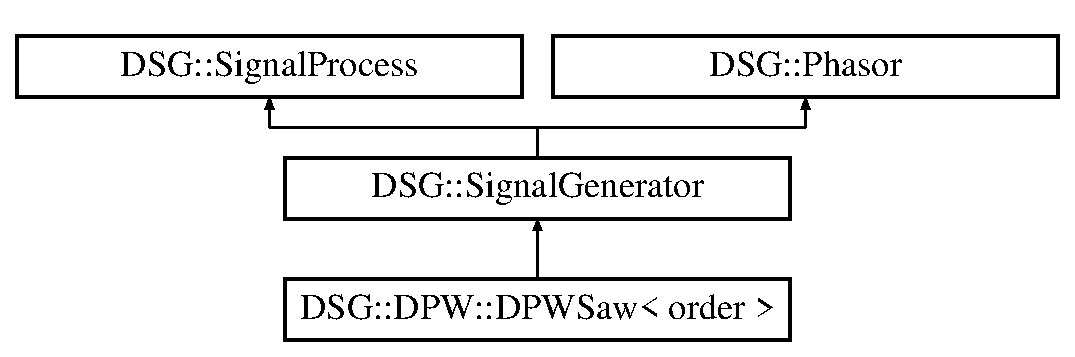
\includegraphics[height=3.000000cm]{class_d_s_g_1_1_d_p_w_1_1_d_p_w_saw}
\end{center}
\end{figure}
\subsection*{Public Member Functions}
\begin{DoxyCompactItemize}
\item 
\hyperlink{class_d_s_g_1_1_d_p_w_1_1_d_p_w_saw_ae9409342bec9d28c6e3e5235619f0c17}{D\+P\+W\+Saw} ()
\item 
\hyperlink{class_d_s_g_1_1_d_p_w_1_1_d_p_w_saw_a750142d70e22ccfb961edc73b13386f6}{D\+P\+W\+Saw} (\hyperlink{namespace_d_s_g_a4315a061386fa1014fda09b15d3a6973}{D\+S\+G\+::\+D\+S\+G\+Frequency} const \&frequency, \hyperlink{namespace_d_s_g_a44431ce1eb0a7300efdd207bc879e52c}{D\+S\+G\+::\+D\+S\+G\+Phase} const \&offset)
\item 
virtual \hyperlink{class_d_s_g_1_1_d_p_w_1_1_d_p_w_saw_afc78ee5a1353dec65adf963a677e95fe}{$\sim$\+D\+P\+W\+Saw} ()
\item 
virtual bool \hyperlink{class_d_s_g_1_1_d_p_w_1_1_d_p_w_saw_a8d0bffad58e9bce19fe737302de749ed}{Perform} (\hyperlink{namespace_d_s_g_ac39a94cd27ebcd9c1e7502d0c624894a}{D\+S\+G\+::\+D\+S\+G\+Sample} \&signal)
\item 
virtual bool \hyperlink{class_d_s_g_1_1_d_p_w_1_1_d_p_w_saw_a03548019c5ec057f5980a4bd99a0d3f0}{Perform} (\hyperlink{class_d_s_g_1_1_ring_buffer}{D\+S\+G\+::\+Ring\+Buffer} \&signal)
\end{DoxyCompactItemize}
\subsection*{Protected Attributes}
\begin{DoxyCompactItemize}
\item 
\hyperlink{namespace_d_s_g_ac39a94cd27ebcd9c1e7502d0c624894a}{D\+S\+G\+::\+D\+S\+G\+Sample} \hyperlink{class_d_s_g_1_1_d_p_w_1_1_d_p_w_saw_a5b9fcbe7361f56358afd2728c5de4014}{\+\_\+register}
\item 
\hyperlink{class_d_s_g_1_1_d_p_w_1_1_d_p_w___differentiator}{D\+S\+G\+::\+D\+P\+W\+::\+D\+P\+W\+\_\+\+Differentiator}\\*
$<$ order $>$ \hyperlink{class_d_s_g_1_1_d_p_w_1_1_d_p_w_saw_af1ded15ce266aa7bd1594de38bba6890}{\+\_\+diff}
\end{DoxyCompactItemize}
\subsection*{Additional Inherited Members}


\subsection{Detailed Description}
\subsubsection*{template$<$unsigned order$>$class D\+S\+G\+::\+D\+P\+W\+::\+D\+P\+W\+Saw$<$ order $>$}

\hyperlink{class_d_s_g_1_1_d_p_w_1_1_d_p_w_saw}{D\+S\+G\+::\+D\+P\+W\+::\+D\+P\+W\+Saw} -\/ Sawtooth Generator using the Nth Order \hyperlink{namespace_d_s_g_1_1_d_p_w}{D\+P\+W} algorithm. 

Definition at line \hyperlink{_d_p_w_saw_8h_source_l00034}{34} of file \hyperlink{_d_p_w_saw_8h_source}{D\+P\+W\+Saw.\+h}.



\subsection{Constructor \& Destructor Documentation}
\hypertarget{class_d_s_g_1_1_d_p_w_1_1_d_p_w_saw_ae9409342bec9d28c6e3e5235619f0c17}{\index{D\+S\+G\+::\+D\+P\+W\+::\+D\+P\+W\+Saw@{D\+S\+G\+::\+D\+P\+W\+::\+D\+P\+W\+Saw}!D\+P\+W\+Saw@{D\+P\+W\+Saw}}
\index{D\+P\+W\+Saw@{D\+P\+W\+Saw}!D\+S\+G\+::\+D\+P\+W\+::\+D\+P\+W\+Saw@{D\+S\+G\+::\+D\+P\+W\+::\+D\+P\+W\+Saw}}
\subsubsection[{D\+P\+W\+Saw}]{\setlength{\rightskip}{0pt plus 5cm}template$<$unsigned order$>$ {\bf D\+S\+G\+::\+D\+P\+W\+::\+D\+P\+W\+Saw}$<$ order $>$\+::{\bf D\+P\+W\+Saw} (
\begin{DoxyParamCaption}
{}
\end{DoxyParamCaption}
)\hspace{0.3cm}{\ttfamily [inline]}}}\label{class_d_s_g_1_1_d_p_w_1_1_d_p_w_saw_ae9409342bec9d28c6e3e5235619f0c17}


Definition at line \hyperlink{_d_p_w_saw_8h_source_l00036}{36} of file \hyperlink{_d_p_w_saw_8h_source}{D\+P\+W\+Saw.\+h}.


\begin{DoxyCode}
00036                     :\hyperlink{class_d_s_g_1_1_signal_generator}{DSG::SignalGenerator}(),\hyperlink{class_d_s_g_1_1_d_p_w_1_1_d_p_w_saw_a5b9fcbe7361f56358afd2728c5de4014}{\_register}(0)\{
00037                 DSG::StaticAssertBounds<1, 6,order>();
00038             \}
\end{DoxyCode}
\hypertarget{class_d_s_g_1_1_d_p_w_1_1_d_p_w_saw_a750142d70e22ccfb961edc73b13386f6}{\index{D\+S\+G\+::\+D\+P\+W\+::\+D\+P\+W\+Saw@{D\+S\+G\+::\+D\+P\+W\+::\+D\+P\+W\+Saw}!D\+P\+W\+Saw@{D\+P\+W\+Saw}}
\index{D\+P\+W\+Saw@{D\+P\+W\+Saw}!D\+S\+G\+::\+D\+P\+W\+::\+D\+P\+W\+Saw@{D\+S\+G\+::\+D\+P\+W\+::\+D\+P\+W\+Saw}}
\subsubsection[{D\+P\+W\+Saw}]{\setlength{\rightskip}{0pt plus 5cm}template$<$unsigned order$>$ {\bf D\+S\+G\+::\+D\+P\+W\+::\+D\+P\+W\+Saw}$<$ order $>$\+::{\bf D\+P\+W\+Saw} (
\begin{DoxyParamCaption}
\item[{{\bf D\+S\+G\+::\+D\+S\+G\+Frequency} const \&}]{frequency, }
\item[{{\bf D\+S\+G\+::\+D\+S\+G\+Phase} const \&}]{offset}
\end{DoxyParamCaption}
)\hspace{0.3cm}{\ttfamily [inline]}}}\label{class_d_s_g_1_1_d_p_w_1_1_d_p_w_saw_a750142d70e22ccfb961edc73b13386f6}


Definition at line \hyperlink{_d_p_w_saw_8h_source_l00039}{39} of file \hyperlink{_d_p_w_saw_8h_source}{D\+P\+W\+Saw.\+h}.


\begin{DoxyCode}
00039 :\hyperlink{class_d_s_g_1_1_signal_generator}{DSG::SignalGenerator}(frequency,offset),\hyperlink{class_d_s_g_1_1_d_p_w_1_1_d_p_w_saw_a5b9fcbe7361f56358afd2728c5de4014}{\_register}(0)\{
      DSG::StaticAssertBounds<1, 6,order>();\}
\end{DoxyCode}
\hypertarget{class_d_s_g_1_1_d_p_w_1_1_d_p_w_saw_afc78ee5a1353dec65adf963a677e95fe}{\index{D\+S\+G\+::\+D\+P\+W\+::\+D\+P\+W\+Saw@{D\+S\+G\+::\+D\+P\+W\+::\+D\+P\+W\+Saw}!````~D\+P\+W\+Saw@{$\sim$\+D\+P\+W\+Saw}}
\index{````~D\+P\+W\+Saw@{$\sim$\+D\+P\+W\+Saw}!D\+S\+G\+::\+D\+P\+W\+::\+D\+P\+W\+Saw@{D\+S\+G\+::\+D\+P\+W\+::\+D\+P\+W\+Saw}}
\subsubsection[{$\sim$\+D\+P\+W\+Saw}]{\setlength{\rightskip}{0pt plus 5cm}template$<$unsigned order$>$ virtual {\bf D\+S\+G\+::\+D\+P\+W\+::\+D\+P\+W\+Saw}$<$ order $>$\+::$\sim${\bf D\+P\+W\+Saw} (
\begin{DoxyParamCaption}
{}
\end{DoxyParamCaption}
)\hspace{0.3cm}{\ttfamily [inline]}, {\ttfamily [virtual]}}}\label{class_d_s_g_1_1_d_p_w_1_1_d_p_w_saw_afc78ee5a1353dec65adf963a677e95fe}


Definition at line \hyperlink{_d_p_w_saw_8h_source_l00040}{40} of file \hyperlink{_d_p_w_saw_8h_source}{D\+P\+W\+Saw.\+h}.


\begin{DoxyCode}
00040 \{\}
\end{DoxyCode}


\subsection{Member Function Documentation}
\hypertarget{class_d_s_g_1_1_d_p_w_1_1_d_p_w_saw_a8d0bffad58e9bce19fe737302de749ed}{\index{D\+S\+G\+::\+D\+P\+W\+::\+D\+P\+W\+Saw@{D\+S\+G\+::\+D\+P\+W\+::\+D\+P\+W\+Saw}!Perform@{Perform}}
\index{Perform@{Perform}!D\+S\+G\+::\+D\+P\+W\+::\+D\+P\+W\+Saw@{D\+S\+G\+::\+D\+P\+W\+::\+D\+P\+W\+Saw}}
\subsubsection[{Perform}]{\setlength{\rightskip}{0pt plus 5cm}template$<$unsigned order$>$ virtual bool {\bf D\+S\+G\+::\+D\+P\+W\+::\+D\+P\+W\+Saw}$<$ order $>$\+::Perform (
\begin{DoxyParamCaption}
\item[{{\bf D\+S\+G\+::\+D\+S\+G\+Sample} \&}]{signal}
\end{DoxyParamCaption}
)\hspace{0.3cm}{\ttfamily [inline]}, {\ttfamily [virtual]}}}\label{class_d_s_g_1_1_d_p_w_1_1_d_p_w_saw_a8d0bffad58e9bce19fe737302de749ed}


Reimplemented from \hyperlink{class_d_s_g_1_1_signal_generator_a46fe75a81a242e191c5049d33ddf4155}{D\+S\+G\+::\+Signal\+Generator}.



Definition at line \hyperlink{_d_p_w_saw_8h_source_l00041}{41} of file \hyperlink{_d_p_w_saw_8h_source}{D\+P\+W\+Saw.\+h}.


\begin{DoxyCode}
00041                                                              \{
00042                 \textcolor{comment}{//trivial saw ramping from -1 to 1}
00043                 \hyperlink{class_d_s_g_1_1_d_p_w_1_1_d_p_w_saw_a5b9fcbe7361f56358afd2728c5de4014}{\_register} = \hyperlink{class_d_s_g_1_1_signal_generator_a1e23eb94e204b11db75fca030b951065}{\_phasor};
00044                 \hyperlink{class_d_s_g_1_1_d_p_w_1_1_d_p_w_saw_a5b9fcbe7361f56358afd2728c5de4014}{\_register}-=0.5;
00045                 \hyperlink{class_d_s_g_1_1_d_p_w_1_1_d_p_w_saw_a5b9fcbe7361f56358afd2728c5de4014}{\_register}*=2.0;
00046                 \textcolor{comment}{/*-------------------------*/}
00047                 \textcolor{comment}{//DPW algorithm}
00048                 \textcolor{comment}{//polynomial shaping}
00049                 \hyperlink{class_d_s_g_1_1_d_p_w_1_1_d_p_w_saw_a5b9fcbe7361f56358afd2728c5de4014}{\_register}=DSG::DPW::DPW\_Polynomial<order>(\hyperlink{class_d_s_g_1_1_d_p_w_1_1_d_p_w_saw_a5b9fcbe7361f56358afd2728c5de4014}{\_register});
00050                 \textcolor{comment}{//differentiating}
00051                 signal = \hyperlink{class_d_s_g_1_1_d_p_w_1_1_d_p_w_saw_af1ded15ce266aa7bd1594de38bba6890}{\_diff}(\hyperlink{class_d_s_g_1_1_d_p_w_1_1_d_p_w_saw_a5b9fcbe7361f56358afd2728c5de4014}{\_register},\hyperlink{class_d_s_g_1_1_signal_generator_a01c046bb52bbb74afd789fdce7978f65}{\_dt});
00052                 \textcolor{comment}{/*-------------------------*/}
00053                 \textcolor{comment}{//signal = DSG::EnforceBounds<-1, 1>(signal);}
00054                 \textcolor{comment}{//advance phase}
00055                 \hyperlink{class_d_s_g_1_1_signal_generator_a4c034c5b9ef3dc7548839288355643d5}{step}();
00056                 \textcolor{keywordflow}{return} \textcolor{keyword}{true};
00057             \}
\end{DoxyCode}
\hypertarget{class_d_s_g_1_1_d_p_w_1_1_d_p_w_saw_a03548019c5ec057f5980a4bd99a0d3f0}{\index{D\+S\+G\+::\+D\+P\+W\+::\+D\+P\+W\+Saw@{D\+S\+G\+::\+D\+P\+W\+::\+D\+P\+W\+Saw}!Perform@{Perform}}
\index{Perform@{Perform}!D\+S\+G\+::\+D\+P\+W\+::\+D\+P\+W\+Saw@{D\+S\+G\+::\+D\+P\+W\+::\+D\+P\+W\+Saw}}
\subsubsection[{Perform}]{\setlength{\rightskip}{0pt plus 5cm}template$<$unsigned order$>$ virtual bool {\bf D\+S\+G\+::\+D\+P\+W\+::\+D\+P\+W\+Saw}$<$ order $>$\+::Perform (
\begin{DoxyParamCaption}
\item[{{\bf D\+S\+G\+::\+Ring\+Buffer} \&}]{signal}
\end{DoxyParamCaption}
)\hspace{0.3cm}{\ttfamily [inline]}, {\ttfamily [virtual]}}}\label{class_d_s_g_1_1_d_p_w_1_1_d_p_w_saw_a03548019c5ec057f5980a4bd99a0d3f0}


Reimplemented from \hyperlink{class_d_s_g_1_1_signal_generator_ab050f80e84e6c8b3e354b56930d6a02b}{D\+S\+G\+::\+Signal\+Generator}.



Definition at line \hyperlink{_d_p_w_saw_8h_source_l00058}{58} of file \hyperlink{_d_p_w_saw_8h_source}{D\+P\+W\+Saw.\+h}.


\begin{DoxyCode}
00058                                                               \{
00059                 signal.\hyperlink{class_d_s_g_1_1_ring_buffer_ab23c8003d2857809a816068eeb209d60}{Flush}();
00060                 \textcolor{keywordflow}{while} (!signal.\hyperlink{class_d_s_g_1_1_ring_buffer_a53ddb04ffcbb5470a8d2b0a3c65b70cb}{Full}()) \{
00061                     \textcolor{keywordflow}{if} (\hyperlink{class_d_s_g_1_1_d_p_w_1_1_d_p_w_saw_a8d0bffad58e9bce19fe737302de749ed}{Perform}(\hyperlink{class_d_s_g_1_1_signal_generator_a28a9b47a1aa0783029f11a19ba0363f2}{\_storage})) \{
00062                         \textcolor{keywordflow}{if}(signal.\hyperlink{class_d_s_g_1_1_ring_buffer_aa5dd2caa0a270173251faee40a43d692}{Write}(\hyperlink{class_d_s_g_1_1_signal_generator_a28a9b47a1aa0783029f11a19ba0363f2}{\_storage}))\{
00063                         \}\textcolor{keywordflow}{else} \textcolor{keywordflow}{return} \textcolor{keyword}{false};
00064                     \}\textcolor{keywordflow}{else} \textcolor{keywordflow}{return} \textcolor{keyword}{false};
00065                 \}\textcolor{keywordflow}{return} \textcolor{keyword}{true};
00066             \}
\end{DoxyCode}


\subsection{Member Data Documentation}
\hypertarget{class_d_s_g_1_1_d_p_w_1_1_d_p_w_saw_af1ded15ce266aa7bd1594de38bba6890}{\index{D\+S\+G\+::\+D\+P\+W\+::\+D\+P\+W\+Saw@{D\+S\+G\+::\+D\+P\+W\+::\+D\+P\+W\+Saw}!\+\_\+diff@{\+\_\+diff}}
\index{\+\_\+diff@{\+\_\+diff}!D\+S\+G\+::\+D\+P\+W\+::\+D\+P\+W\+Saw@{D\+S\+G\+::\+D\+P\+W\+::\+D\+P\+W\+Saw}}
\subsubsection[{\+\_\+diff}]{\setlength{\rightskip}{0pt plus 5cm}template$<$unsigned order$>$ {\bf D\+S\+G\+::\+D\+P\+W\+::\+D\+P\+W\+\_\+\+Differentiator}$<$order$>$ {\bf D\+S\+G\+::\+D\+P\+W\+::\+D\+P\+W\+Saw}$<$ order $>$\+::\+\_\+diff\hspace{0.3cm}{\ttfamily [protected]}}}\label{class_d_s_g_1_1_d_p_w_1_1_d_p_w_saw_af1ded15ce266aa7bd1594de38bba6890}


Definition at line \hyperlink{_d_p_w_saw_8h_source_l00069}{69} of file \hyperlink{_d_p_w_saw_8h_source}{D\+P\+W\+Saw.\+h}.

\hypertarget{class_d_s_g_1_1_d_p_w_1_1_d_p_w_saw_a5b9fcbe7361f56358afd2728c5de4014}{\index{D\+S\+G\+::\+D\+P\+W\+::\+D\+P\+W\+Saw@{D\+S\+G\+::\+D\+P\+W\+::\+D\+P\+W\+Saw}!\+\_\+register@{\+\_\+register}}
\index{\+\_\+register@{\+\_\+register}!D\+S\+G\+::\+D\+P\+W\+::\+D\+P\+W\+Saw@{D\+S\+G\+::\+D\+P\+W\+::\+D\+P\+W\+Saw}}
\subsubsection[{\+\_\+register}]{\setlength{\rightskip}{0pt plus 5cm}template$<$unsigned order$>$ {\bf D\+S\+G\+::\+D\+S\+G\+Sample} {\bf D\+S\+G\+::\+D\+P\+W\+::\+D\+P\+W\+Saw}$<$ order $>$\+::\+\_\+register\hspace{0.3cm}{\ttfamily [protected]}}}\label{class_d_s_g_1_1_d_p_w_1_1_d_p_w_saw_a5b9fcbe7361f56358afd2728c5de4014}


Definition at line \hyperlink{_d_p_w_saw_8h_source_l00068}{68} of file \hyperlink{_d_p_w_saw_8h_source}{D\+P\+W\+Saw.\+h}.



The documentation for this class was generated from the following file\+:\begin{DoxyCompactItemize}
\item 
\hyperlink{_d_p_w_saw_8h}{D\+P\+W\+Saw.\+h}\end{DoxyCompactItemize}

\hypertarget{class_d_s_g_1_1_e_p_t_r_1_1_e_p_t_r_saw}{\section{D\+S\+G\+:\+:E\+P\+T\+R\+:\+:E\+P\+T\+R\+Saw Class Reference}
\label{class_d_s_g_1_1_e_p_t_r_1_1_e_p_t_r_saw}\index{D\+S\+G\+::\+E\+P\+T\+R\+::\+E\+P\+T\+R\+Saw@{D\+S\+G\+::\+E\+P\+T\+R\+::\+E\+P\+T\+R\+Saw}}
}


\hyperlink{class_d_s_g_1_1_e_p_t_r_1_1_e_p_t_r_saw}{D\+S\+G\+::\+E\+P\+T\+R\+::\+E\+P\+T\+R\+Saw}-\/\+Sawtooth Wave Generator Using The Efficienct Polynomial Transfer Region Algorithm.  




{\ttfamily \#include $<$E\+P\+T\+R\+Saw.\+h$>$}

Inheritance diagram for D\+S\+G\+:\+:E\+P\+T\+R\+:\+:E\+P\+T\+R\+Saw\+:\begin{figure}[H]
\begin{center}
\leavevmode
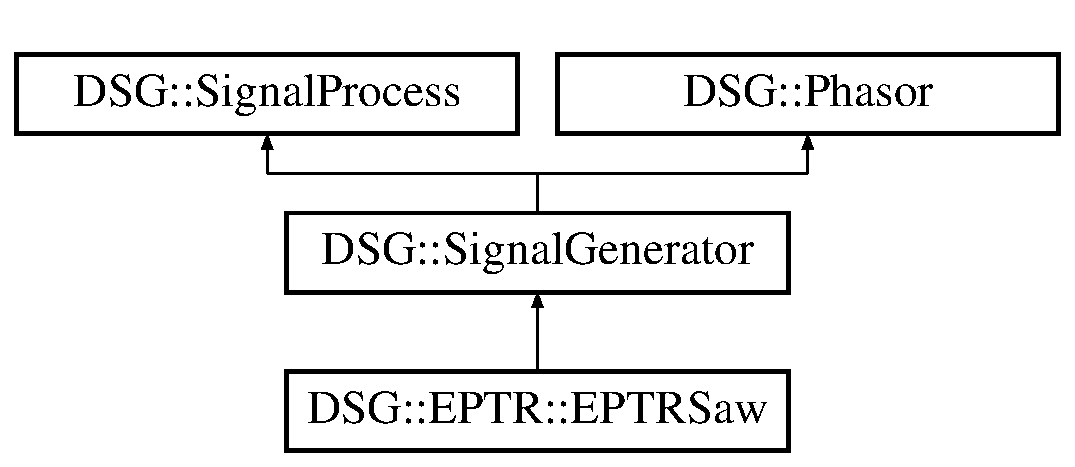
\includegraphics[height=3.000000cm]{class_d_s_g_1_1_e_p_t_r_1_1_e_p_t_r_saw}
\end{center}
\end{figure}
\subsection*{Public Member Functions}
\begin{DoxyCompactItemize}
\item 
\hyperlink{class_d_s_g_1_1_e_p_t_r_1_1_e_p_t_r_saw_a65c2009548fb7f946d48ea794c830501}{E\+P\+T\+R\+Saw} ()
\item 
\hyperlink{class_d_s_g_1_1_e_p_t_r_1_1_e_p_t_r_saw_a3a571a16f3ef0e230db2daa0cd249855}{E\+P\+T\+R\+Saw} (\hyperlink{namespace_d_s_g_a4315a061386fa1014fda09b15d3a6973}{D\+S\+G\+::\+D\+S\+G\+Frequency} const \&frequency, \hyperlink{namespace_d_s_g_a44431ce1eb0a7300efdd207bc879e52c}{D\+S\+G\+::\+D\+S\+G\+Phase} const \&offset)
\item 
virtual \hyperlink{class_d_s_g_1_1_e_p_t_r_1_1_e_p_t_r_saw_a932fb8ef2df61ed06e6cca5cdc622884}{$\sim$\+E\+P\+T\+R\+Saw} ()
\item 
virtual bool \hyperlink{class_d_s_g_1_1_e_p_t_r_1_1_e_p_t_r_saw_aa253efa41cca56f334ccb0fd32c2cd56}{Perform} (\hyperlink{namespace_d_s_g_ac39a94cd27ebcd9c1e7502d0c624894a}{D\+S\+G\+::\+D\+S\+G\+Sample} \&signal)
\item 
virtual bool \hyperlink{class_d_s_g_1_1_e_p_t_r_1_1_e_p_t_r_saw_a9dbefaeeb74e30e722bb5d8ea767cdca}{Perform} (\hyperlink{class_d_s_g_1_1_ring_buffer}{D\+S\+G\+::\+Ring\+Buffer} \&signal)
\end{DoxyCompactItemize}
\subsection*{Protected Attributes}
\begin{DoxyCompactItemize}
\item 
\hyperlink{namespace_d_s_g_ac39a94cd27ebcd9c1e7502d0c624894a}{D\+S\+G\+::\+D\+S\+G\+Sample} \hyperlink{class_d_s_g_1_1_e_p_t_r_1_1_e_p_t_r_saw_a38d89a4557f487e0e447e1da6acf7e5f}{\+\_\+register}
\end{DoxyCompactItemize}
\subsection*{Additional Inherited Members}


\subsection{Detailed Description}
\hyperlink{class_d_s_g_1_1_e_p_t_r_1_1_e_p_t_r_saw}{D\+S\+G\+::\+E\+P\+T\+R\+::\+E\+P\+T\+R\+Saw}-\/\+Sawtooth Wave Generator Using The Efficienct Polynomial Transfer Region Algorithm. 

\begin{DoxyRefDesc}{Todo}
\item[\hyperlink{todo__todo000006}{Todo}]Test and Possibly Re-\/\+Write \hyperlink{class_d_s_g_1_1_e_p_t_r_1_1_e_p_t_r_saw}{D\+S\+G\+::\+E\+P\+T\+R\+::\+E\+P\+T\+R\+Saw} algorithm \end{DoxyRefDesc}


Definition at line \hyperlink{_e_p_t_r_saw_8h_source_l00035}{35} of file \hyperlink{_e_p_t_r_saw_8h_source}{E\+P\+T\+R\+Saw.\+h}.



\subsection{Constructor \& Destructor Documentation}
\hypertarget{class_d_s_g_1_1_e_p_t_r_1_1_e_p_t_r_saw_a65c2009548fb7f946d48ea794c830501}{\index{D\+S\+G\+::\+E\+P\+T\+R\+::\+E\+P\+T\+R\+Saw@{D\+S\+G\+::\+E\+P\+T\+R\+::\+E\+P\+T\+R\+Saw}!E\+P\+T\+R\+Saw@{E\+P\+T\+R\+Saw}}
\index{E\+P\+T\+R\+Saw@{E\+P\+T\+R\+Saw}!D\+S\+G\+::\+E\+P\+T\+R\+::\+E\+P\+T\+R\+Saw@{D\+S\+G\+::\+E\+P\+T\+R\+::\+E\+P\+T\+R\+Saw}}
\subsubsection[{E\+P\+T\+R\+Saw}]{\setlength{\rightskip}{0pt plus 5cm}D\+S\+G\+::\+E\+P\+T\+R\+::\+E\+P\+T\+R\+Saw\+::\+E\+P\+T\+R\+Saw (
\begin{DoxyParamCaption}
{}
\end{DoxyParamCaption}
)}}\label{class_d_s_g_1_1_e_p_t_r_1_1_e_p_t_r_saw_a65c2009548fb7f946d48ea794c830501}


Definition at line \hyperlink{_e_p_t_r_saw_8cpp_source_l00025}{25} of file \hyperlink{_e_p_t_r_saw_8cpp_source}{E\+P\+T\+R\+Saw.\+cpp}.


\begin{DoxyCode}
00025 :\hyperlink{class_d_s_g_1_1_signal_generator}{DSG::SignalGenerator}()\{\}
\end{DoxyCode}
\hypertarget{class_d_s_g_1_1_e_p_t_r_1_1_e_p_t_r_saw_a3a571a16f3ef0e230db2daa0cd249855}{\index{D\+S\+G\+::\+E\+P\+T\+R\+::\+E\+P\+T\+R\+Saw@{D\+S\+G\+::\+E\+P\+T\+R\+::\+E\+P\+T\+R\+Saw}!E\+P\+T\+R\+Saw@{E\+P\+T\+R\+Saw}}
\index{E\+P\+T\+R\+Saw@{E\+P\+T\+R\+Saw}!D\+S\+G\+::\+E\+P\+T\+R\+::\+E\+P\+T\+R\+Saw@{D\+S\+G\+::\+E\+P\+T\+R\+::\+E\+P\+T\+R\+Saw}}
\subsubsection[{E\+P\+T\+R\+Saw}]{\setlength{\rightskip}{0pt plus 5cm}D\+S\+G\+::\+E\+P\+T\+R\+::\+E\+P\+T\+R\+Saw\+::\+E\+P\+T\+R\+Saw (
\begin{DoxyParamCaption}
\item[{{\bf D\+S\+G\+::\+D\+S\+G\+Frequency} const \&}]{frequency, }
\item[{{\bf D\+S\+G\+::\+D\+S\+G\+Phase} const \&}]{offset}
\end{DoxyParamCaption}
)}}\label{class_d_s_g_1_1_e_p_t_r_1_1_e_p_t_r_saw_a3a571a16f3ef0e230db2daa0cd249855}


Definition at line \hyperlink{_e_p_t_r_saw_8cpp_source_l00026}{26} of file \hyperlink{_e_p_t_r_saw_8cpp_source}{E\+P\+T\+R\+Saw.\+cpp}.


\begin{DoxyCode}
00026 :\hyperlink{class_d_s_g_1_1_signal_generator}{DSG::SignalGenerator}(frequency,offset)\{\}
\end{DoxyCode}
\hypertarget{class_d_s_g_1_1_e_p_t_r_1_1_e_p_t_r_saw_a932fb8ef2df61ed06e6cca5cdc622884}{\index{D\+S\+G\+::\+E\+P\+T\+R\+::\+E\+P\+T\+R\+Saw@{D\+S\+G\+::\+E\+P\+T\+R\+::\+E\+P\+T\+R\+Saw}!````~E\+P\+T\+R\+Saw@{$\sim$\+E\+P\+T\+R\+Saw}}
\index{````~E\+P\+T\+R\+Saw@{$\sim$\+E\+P\+T\+R\+Saw}!D\+S\+G\+::\+E\+P\+T\+R\+::\+E\+P\+T\+R\+Saw@{D\+S\+G\+::\+E\+P\+T\+R\+::\+E\+P\+T\+R\+Saw}}
\subsubsection[{$\sim$\+E\+P\+T\+R\+Saw}]{\setlength{\rightskip}{0pt plus 5cm}D\+S\+G\+::\+E\+P\+T\+R\+::\+E\+P\+T\+R\+Saw\+::$\sim$\+E\+P\+T\+R\+Saw (
\begin{DoxyParamCaption}
{}
\end{DoxyParamCaption}
)\hspace{0.3cm}{\ttfamily [virtual]}}}\label{class_d_s_g_1_1_e_p_t_r_1_1_e_p_t_r_saw_a932fb8ef2df61ed06e6cca5cdc622884}


Definition at line \hyperlink{_e_p_t_r_saw_8cpp_source_l00027}{27} of file \hyperlink{_e_p_t_r_saw_8cpp_source}{E\+P\+T\+R\+Saw.\+cpp}.


\begin{DoxyCode}
00027 \{\}\end{DoxyCode}


\subsection{Member Function Documentation}
\hypertarget{class_d_s_g_1_1_e_p_t_r_1_1_e_p_t_r_saw_aa253efa41cca56f334ccb0fd32c2cd56}{\index{D\+S\+G\+::\+E\+P\+T\+R\+::\+E\+P\+T\+R\+Saw@{D\+S\+G\+::\+E\+P\+T\+R\+::\+E\+P\+T\+R\+Saw}!Perform@{Perform}}
\index{Perform@{Perform}!D\+S\+G\+::\+E\+P\+T\+R\+::\+E\+P\+T\+R\+Saw@{D\+S\+G\+::\+E\+P\+T\+R\+::\+E\+P\+T\+R\+Saw}}
\subsubsection[{Perform}]{\setlength{\rightskip}{0pt plus 5cm}bool D\+S\+G\+::\+E\+P\+T\+R\+::\+E\+P\+T\+R\+Saw\+::\+Perform (
\begin{DoxyParamCaption}
\item[{{\bf D\+S\+G\+::\+D\+S\+G\+Sample} \&}]{signal}
\end{DoxyParamCaption}
)\hspace{0.3cm}{\ttfamily [inline]}, {\ttfamily [virtual]}}}\label{class_d_s_g_1_1_e_p_t_r_1_1_e_p_t_r_saw_aa253efa41cca56f334ccb0fd32c2cd56}


Reimplemented from \hyperlink{class_d_s_g_1_1_signal_generator_a46fe75a81a242e191c5049d33ddf4155}{D\+S\+G\+::\+Signal\+Generator}.



Definition at line \hyperlink{_e_p_t_r_saw_8h_source_l00045}{45} of file \hyperlink{_e_p_t_r_saw_8h_source}{E\+P\+T\+R\+Saw.\+h}.


\begin{DoxyCode}
00045                                                                \{
00046 \textcolor{preprocessor}{#ifdef \_\_APPLE\_\_}
00047 \textcolor{preprocessor}{#warning Untested For Aliasing DSG::EPTR::EPTRSaw::Perform()}
00048 \textcolor{preprocessor}{#endif}
00049             \textcolor{comment}{//generate trivial saw}
00050             \hyperlink{class_d_s_g_1_1_e_p_t_r_1_1_e_p_t_r_saw_a38d89a4557f487e0e447e1da6acf7e5f}{\_register} = \hyperlink{class_d_s_g_1_1_phasor_a82c148d71128cfc518fc8e7e131c3a38}{\_phasor};
00051             \hyperlink{class_d_s_g_1_1_e_p_t_r_1_1_e_p_t_r_saw_a38d89a4557f487e0e447e1da6acf7e5f}{\_register}+=0.5;
00052             \textcolor{keywordflow}{if} (\hyperlink{class_d_s_g_1_1_e_p_t_r_1_1_e_p_t_r_saw_a38d89a4557f487e0e447e1da6acf7e5f}{\_register}>1.0) \{
00053                 --\hyperlink{class_d_s_g_1_1_e_p_t_r_1_1_e_p_t_r_saw_a38d89a4557f487e0e447e1da6acf7e5f}{\_register};
00054             \}
00055             \hyperlink{class_d_s_g_1_1_e_p_t_r_1_1_e_p_t_r_saw_a38d89a4557f487e0e447e1da6acf7e5f}{\_register}-=0.5;
00056             \hyperlink{class_d_s_g_1_1_e_p_t_r_1_1_e_p_t_r_saw_a38d89a4557f487e0e447e1da6acf7e5f}{\_register}*=2.0;
00057             \textcolor{keywordflow}{if} (\hyperlink{class_d_s_g_1_1_e_p_t_r_1_1_e_p_t_r_saw_a38d89a4557f487e0e447e1da6acf7e5f}{\_register} > 1.0-\hyperlink{class_d_s_g_1_1_phasor_afaaa3559b6cd84535c10ff896148c6bd}{\_dt}) \{
00058                 \textcolor{comment}{//transition region detected}
00059                 \textcolor{comment}{//apply eptr correction}
00060                 signal = \hyperlink{class_d_s_g_1_1_e_p_t_r_1_1_e_p_t_r_saw_a38d89a4557f487e0e447e1da6acf7e5f}{\_register} - (\hyperlink{class_d_s_g_1_1_e_p_t_r_1_1_e_p_t_r_saw_a38d89a4557f487e0e447e1da6acf7e5f}{\_register}/\hyperlink{class_d_s_g_1_1_phasor_afaaa3559b6cd84535c10ff896148c6bd}{\_dt}) + (1.0/
      \hyperlink{class_d_s_g_1_1_phasor_afaaa3559b6cd84535c10ff896148c6bd}{\_dt}) -1;
00061             \}\textcolor{keywordflow}{else}\{
00062                 signal = \hyperlink{class_d_s_g_1_1_e_p_t_r_1_1_e_p_t_r_saw_a38d89a4557f487e0e447e1da6acf7e5f}{\_register};
00063             \}
00064             \hyperlink{class_d_s_g_1_1_phasor_a6a088b29e506fb5e99d73f4f0160c583}{step}();\textcolor{comment}{//avance phase}
00065             \textcolor{keywordflow}{return} \textcolor{keyword}{true};
00066         \}
\end{DoxyCode}
\hypertarget{class_d_s_g_1_1_e_p_t_r_1_1_e_p_t_r_saw_a9dbefaeeb74e30e722bb5d8ea767cdca}{\index{D\+S\+G\+::\+E\+P\+T\+R\+::\+E\+P\+T\+R\+Saw@{D\+S\+G\+::\+E\+P\+T\+R\+::\+E\+P\+T\+R\+Saw}!Perform@{Perform}}
\index{Perform@{Perform}!D\+S\+G\+::\+E\+P\+T\+R\+::\+E\+P\+T\+R\+Saw@{D\+S\+G\+::\+E\+P\+T\+R\+::\+E\+P\+T\+R\+Saw}}
\subsubsection[{Perform}]{\setlength{\rightskip}{0pt plus 5cm}bool D\+S\+G\+::\+E\+P\+T\+R\+::\+E\+P\+T\+R\+Saw\+::\+Perform (
\begin{DoxyParamCaption}
\item[{{\bf D\+S\+G\+::\+Ring\+Buffer} \&}]{signal}
\end{DoxyParamCaption}
)\hspace{0.3cm}{\ttfamily [inline]}, {\ttfamily [virtual]}}}\label{class_d_s_g_1_1_e_p_t_r_1_1_e_p_t_r_saw_a9dbefaeeb74e30e722bb5d8ea767cdca}


Reimplemented from \hyperlink{class_d_s_g_1_1_signal_generator_ab050f80e84e6c8b3e354b56930d6a02b}{D\+S\+G\+::\+Signal\+Generator}.



Definition at line \hyperlink{_e_p_t_r_saw_8h_source_l00067}{67} of file \hyperlink{_e_p_t_r_saw_8h_source}{E\+P\+T\+R\+Saw.\+h}.


\begin{DoxyCode}
00067                                                                 \{
00068             signal.\hyperlink{class_d_s_g_1_1_ring_buffer_ab23c8003d2857809a816068eeb209d60}{Flush}();
00069             \textcolor{keywordflow}{while} (!signal.\hyperlink{class_d_s_g_1_1_ring_buffer_a53ddb04ffcbb5470a8d2b0a3c65b70cb}{Full}()) \{
00070                 \textcolor{keywordflow}{if} (\hyperlink{class_d_s_g_1_1_e_p_t_r_1_1_e_p_t_r_saw_aa253efa41cca56f334ccb0fd32c2cd56}{Perform}(\hyperlink{class_d_s_g_1_1_signal_generator_a28a9b47a1aa0783029f11a19ba0363f2}{\_storage})) \{
00071                     \textcolor{keywordflow}{if}(signal.\hyperlink{class_d_s_g_1_1_ring_buffer_aa5dd2caa0a270173251faee40a43d692}{Write}(\hyperlink{class_d_s_g_1_1_signal_generator_a28a9b47a1aa0783029f11a19ba0363f2}{\_storage}))\{
00072                     \}\textcolor{keywordflow}{else} \textcolor{keywordflow}{return} \textcolor{keyword}{false};
00073                 \}\textcolor{keywordflow}{else} \textcolor{keywordflow}{return} \textcolor{keyword}{false};
00074             \}\textcolor{keywordflow}{return} \textcolor{keyword}{true};
00075         \}
\end{DoxyCode}


\subsection{Member Data Documentation}
\hypertarget{class_d_s_g_1_1_e_p_t_r_1_1_e_p_t_r_saw_a38d89a4557f487e0e447e1da6acf7e5f}{\index{D\+S\+G\+::\+E\+P\+T\+R\+::\+E\+P\+T\+R\+Saw@{D\+S\+G\+::\+E\+P\+T\+R\+::\+E\+P\+T\+R\+Saw}!\+\_\+register@{\+\_\+register}}
\index{\+\_\+register@{\+\_\+register}!D\+S\+G\+::\+E\+P\+T\+R\+::\+E\+P\+T\+R\+Saw@{D\+S\+G\+::\+E\+P\+T\+R\+::\+E\+P\+T\+R\+Saw}}
\subsubsection[{\+\_\+register}]{\setlength{\rightskip}{0pt plus 5cm}{\bf D\+S\+G\+::\+D\+S\+G\+Sample} D\+S\+G\+::\+E\+P\+T\+R\+::\+E\+P\+T\+R\+Saw\+::\+\_\+register\hspace{0.3cm}{\ttfamily [protected]}}}\label{class_d_s_g_1_1_e_p_t_r_1_1_e_p_t_r_saw_a38d89a4557f487e0e447e1da6acf7e5f}


Definition at line \hyperlink{_e_p_t_r_saw_8h_source_l00043}{43} of file \hyperlink{_e_p_t_r_saw_8h_source}{E\+P\+T\+R\+Saw.\+h}.



The documentation for this class was generated from the following files\+:\begin{DoxyCompactItemize}
\item 
\hyperlink{_e_p_t_r_saw_8h}{E\+P\+T\+R\+Saw.\+h}\item 
\hyperlink{_e_p_t_r_saw_8cpp}{E\+P\+T\+R\+Saw.\+cpp}\end{DoxyCompactItemize}

\hypertarget{struct_d_s_g_1_1_factorial}{\section{D\+S\+G\+:\+:Factorial$<$ N $>$ Struct Template Reference}
\label{struct_d_s_g_1_1_factorial}\index{D\+S\+G\+::\+Factorial$<$ N $>$@{D\+S\+G\+::\+Factorial$<$ N $>$}}
}


\hyperlink{struct_d_s_g_1_1_factorial}{D\+S\+G\+::\+Factorial} -\/ Compute integer factorial.  




{\ttfamily \#include $<$D\+S\+G\+Math.\+h$>$}

\subsection*{Public Types}
\begin{DoxyCompactItemize}
\item 
enum \{ \hyperlink{struct_d_s_g_1_1_factorial_a2443a477420ba8fc5494b186a58dcaccaebc078d57d6fc1fbd5953d284c9cde04}{value} = N $\ast$ Factorial$<$N-\/1$>$\+:\+:value
 \}
\end{DoxyCompactItemize}


\subsection{Detailed Description}
\subsubsection*{template$<$unsigned long N$>$struct D\+S\+G\+::\+Factorial$<$ N $>$}

\hyperlink{struct_d_s_g_1_1_factorial}{D\+S\+G\+::\+Factorial} -\/ Compute integer factorial. 

Definition at line \hyperlink{_d_s_g_math_8h_source_l00020}{20} of file \hyperlink{_d_s_g_math_8h_source}{D\+S\+G\+Math.\+h}.



\subsection{Member Enumeration Documentation}
\hypertarget{struct_d_s_g_1_1_factorial_a2443a477420ba8fc5494b186a58dcacc}{\subsubsection[{anonymous enum}]{\setlength{\rightskip}{0pt plus 5cm}template$<$unsigned long N$>$ anonymous enum}}\label{struct_d_s_g_1_1_factorial_a2443a477420ba8fc5494b186a58dcacc}
\begin{Desc}
\item[Enumerator]\par
\begin{description}
\index{value@{value}!D\+S\+G\+::\+Factorial@{D\+S\+G\+::\+Factorial}}\index{D\+S\+G\+::\+Factorial@{D\+S\+G\+::\+Factorial}!value@{value}}\item[{\em 
\hypertarget{struct_d_s_g_1_1_factorial_a2443a477420ba8fc5494b186a58dcaccaebc078d57d6fc1fbd5953d284c9cde04}{value}\label{struct_d_s_g_1_1_factorial_a2443a477420ba8fc5494b186a58dcaccaebc078d57d6fc1fbd5953d284c9cde04}
}]\end{description}
\end{Desc}


Definition at line \hyperlink{_d_s_g_math_8h_source_l00021}{21} of file \hyperlink{_d_s_g_math_8h_source}{D\+S\+G\+Math.\+h}.


\begin{DoxyCode}
00021 \{\hyperlink{struct_d_s_g_1_1_factorial_a2443a477420ba8fc5494b186a58dcaccaebc078d57d6fc1fbd5953d284c9cde04}{value} = N * Factorial<N-1>\hyperlink{struct_d_s_g_1_1_factorial_a2443a477420ba8fc5494b186a58dcaccaebc078d57d6fc1fbd5953d284c9cde04}{::value}\};
\end{DoxyCode}


The documentation for this struct was generated from the following file\+:\begin{DoxyCompactItemize}
\item 
/\+Users/alexanderzywicki/\+Documents/\+D\+S\+G/src/\hyperlink{_d_s_g_math_8h}{D\+S\+G\+Math.\+h}\end{DoxyCompactItemize}

\hypertarget{struct_d_s_g_1_1_factorial_3_010_01_4}{\section{D\+S\+G\+:\+:Factorial$<$ 0 $>$ Struct Template Reference}
\label{struct_d_s_g_1_1_factorial_3_010_01_4}\index{D\+S\+G\+::\+Factorial$<$ 0 $>$@{D\+S\+G\+::\+Factorial$<$ 0 $>$}}
}


\hyperlink{struct_d_s_g_1_1_factorial}{D\+S\+G\+::\+Factorial} -\/ Compute integer factorial.  




{\ttfamily \#include $<$D\+S\+G\+Math.\+h$>$}

\subsection*{Public Types}
\begin{DoxyCompactItemize}
\item 
enum \{ \hyperlink{struct_d_s_g_1_1_factorial_3_010_01_4_a6bfe1b9c1bfc0bdeaceb03842acb1927abba93a0ae84b21f3c62dd8baa14039eb}{value} = 1
 \}
\end{DoxyCompactItemize}


\subsection{Detailed Description}
\subsubsection*{template$<$$>$struct D\+S\+G\+::\+Factorial$<$ 0 $>$}

\hyperlink{struct_d_s_g_1_1_factorial}{D\+S\+G\+::\+Factorial} -\/ Compute integer factorial. 

Definition at line \hyperlink{_d_s_g_math_8h_source_l00041}{41} of file \hyperlink{_d_s_g_math_8h_source}{D\+S\+G\+Math.\+h}.



\subsection{Member Enumeration Documentation}
\hypertarget{struct_d_s_g_1_1_factorial_3_010_01_4_a6bfe1b9c1bfc0bdeaceb03842acb1927}{\subsubsection[{anonymous enum}]{\setlength{\rightskip}{0pt plus 5cm}anonymous enum}}\label{struct_d_s_g_1_1_factorial_3_010_01_4_a6bfe1b9c1bfc0bdeaceb03842acb1927}
\begin{Desc}
\item[Enumerator]\par
\begin{description}
\index{value@{value}!D\+S\+G\+::\+Factorial$<$ 0 $>$@{D\+S\+G\+::\+Factorial$<$ 0 $>$}}\index{D\+S\+G\+::\+Factorial$<$ 0 $>$@{D\+S\+G\+::\+Factorial$<$ 0 $>$}!value@{value}}\item[{\em 
\hypertarget{struct_d_s_g_1_1_factorial_3_010_01_4_a6bfe1b9c1bfc0bdeaceb03842acb1927abba93a0ae84b21f3c62dd8baa14039eb}{value}\label{struct_d_s_g_1_1_factorial_3_010_01_4_a6bfe1b9c1bfc0bdeaceb03842acb1927abba93a0ae84b21f3c62dd8baa14039eb}
}]\end{description}
\end{Desc}


Definition at line \hyperlink{_d_s_g_math_8h_source_l00042}{42} of file \hyperlink{_d_s_g_math_8h_source}{D\+S\+G\+Math.\+h}.


\begin{DoxyCode}
00042 \{ \hyperlink{struct_d_s_g_1_1_factorial_3_010_01_4_a6bfe1b9c1bfc0bdeaceb03842acb1927abba93a0ae84b21f3c62dd8baa14039eb}{value} = 1 \};
\end{DoxyCode}


The documentation for this struct was generated from the following file\+:\begin{DoxyCompactItemize}
\item 
\hyperlink{_d_s_g_math_8h}{D\+S\+G\+Math.\+h}\end{DoxyCompactItemize}

\hypertarget{class_d_s_g_1_1_filter_1_1_filter_base}{\section{D\+S\+G\+:\+:Filter\+:\+:Filter\+Base Class Reference}
\label{class_d_s_g_1_1_filter_1_1_filter_base}\index{D\+S\+G\+::\+Filter\+::\+Filter\+Base@{D\+S\+G\+::\+Filter\+::\+Filter\+Base}}
}


\hyperlink{class_d_s_g_1_1_filter_1_1_filter_base}{D\+S\+G\+::\+Filter\+::\+Filter\+Base} -\/ \hyperlink{namespace_d_s_g_1_1_filter}{Filter} Base Class, implements interface for cutoff frequency.  




{\ttfamily \#include $<$Filter.\+h$>$}

Inheritance diagram for D\+S\+G\+:\+:Filter\+:\+:Filter\+Base\+:\begin{figure}[H]
\begin{center}
\leavevmode
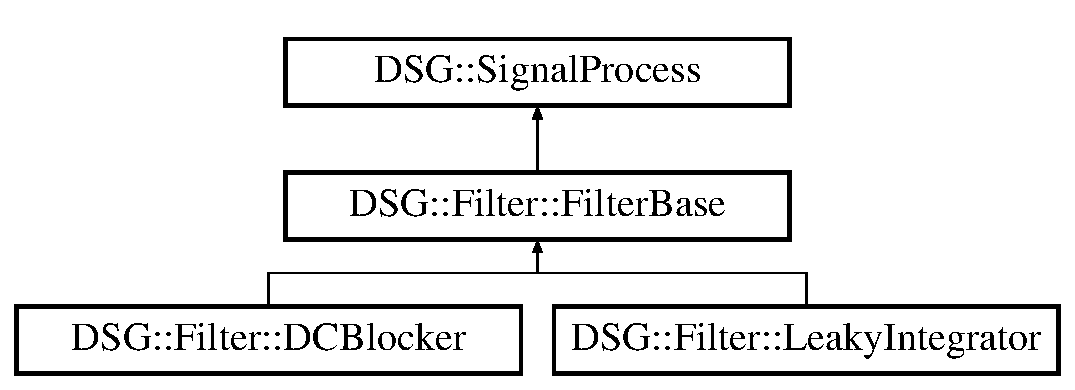
\includegraphics[height=3.000000cm]{class_d_s_g_1_1_filter_1_1_filter_base}
\end{center}
\end{figure}
\subsection*{Public Member Functions}
\begin{DoxyCompactItemize}
\item 
\hyperlink{class_d_s_g_1_1_filter_1_1_filter_base_accc0a6729e252abaa24ad7f72b2f351d}{Filter\+Base} ()
\item 
virtual \hyperlink{class_d_s_g_1_1_filter_1_1_filter_base_a1e220c7fe383eba4822f3896d8b2c2b2}{$\sim$\+Filter\+Base} ()
\item 
virtual bool \hyperlink{class_d_s_g_1_1_filter_1_1_filter_base_ae7b6f59f5408ecab3ccd6c4e723c70b4}{Perform} (\hyperlink{namespace_d_s_g_ac39a94cd27ebcd9c1e7502d0c624894a}{D\+S\+G\+::\+D\+S\+G\+Sample} \&signal)
\item 
virtual bool \hyperlink{class_d_s_g_1_1_filter_1_1_filter_base_aef58742a1362b7ef94574a16036b7109}{Perform} (\hyperlink{class_d_s_g_1_1_ring_buffer}{D\+S\+G\+::\+Ring\+Buffer} \&signal)
\item 
virtual bool \hyperlink{class_d_s_g_1_1_filter_1_1_filter_base_a1bf981bd2ca2151791d91b80dda827fe}{Cutoff} (\hyperlink{namespace_d_s_g_a4315a061386fa1014fda09b15d3a6973}{D\+S\+G\+::\+D\+S\+G\+Frequency} const \&cutoff)
\end{DoxyCompactItemize}
\subsection*{Protected Attributes}
\begin{DoxyCompactItemize}
\item 
\hyperlink{namespace_d_s_g_ac39a94cd27ebcd9c1e7502d0c624894a}{D\+S\+G\+::\+D\+S\+G\+Sample} \hyperlink{class_d_s_g_1_1_filter_1_1_filter_base_a9e21e909fa2989adb88eedcb194e0150}{\+\_\+temp}
\item 
unsigned long \hyperlink{class_d_s_g_1_1_filter_1_1_filter_base_a74068413169f9acb3fcf8276074e3b1d}{count}
\end{DoxyCompactItemize}


\subsection{Detailed Description}
\hyperlink{class_d_s_g_1_1_filter_1_1_filter_base}{D\+S\+G\+::\+Filter\+::\+Filter\+Base} -\/ \hyperlink{namespace_d_s_g_1_1_filter}{Filter} Base Class, implements interface for cutoff frequency. 

Definition at line \hyperlink{_filter_8h_source_l00034}{34} of file \hyperlink{_filter_8h_source}{Filter.\+h}.



\subsection{Constructor \& Destructor Documentation}
\hypertarget{class_d_s_g_1_1_filter_1_1_filter_base_accc0a6729e252abaa24ad7f72b2f351d}{\index{D\+S\+G\+::\+Filter\+::\+Filter\+Base@{D\+S\+G\+::\+Filter\+::\+Filter\+Base}!Filter\+Base@{Filter\+Base}}
\index{Filter\+Base@{Filter\+Base}!D\+S\+G\+::\+Filter\+::\+Filter\+Base@{D\+S\+G\+::\+Filter\+::\+Filter\+Base}}
\subsubsection[{Filter\+Base}]{\setlength{\rightskip}{0pt plus 5cm}D\+S\+G\+::\+Filter\+::\+Filter\+Base\+::\+Filter\+Base (
\begin{DoxyParamCaption}
{}
\end{DoxyParamCaption}
)}}\label{class_d_s_g_1_1_filter_1_1_filter_base_accc0a6729e252abaa24ad7f72b2f351d}


Definition at line \hyperlink{_filter_8cpp_source_l00025}{25} of file \hyperlink{_filter_8cpp_source}{Filter.\+cpp}.


\begin{DoxyCode}
00025 :\hyperlink{class_d_s_g_1_1_filter_1_1_filter_base_a9e21e909fa2989adb88eedcb194e0150}{\_temp}(0),\hyperlink{class_d_s_g_1_1_filter_1_1_filter_base_a74068413169f9acb3fcf8276074e3b1d}{count}(0)\{\}
\end{DoxyCode}
\hypertarget{class_d_s_g_1_1_filter_1_1_filter_base_a1e220c7fe383eba4822f3896d8b2c2b2}{\index{D\+S\+G\+::\+Filter\+::\+Filter\+Base@{D\+S\+G\+::\+Filter\+::\+Filter\+Base}!````~Filter\+Base@{$\sim$\+Filter\+Base}}
\index{````~Filter\+Base@{$\sim$\+Filter\+Base}!D\+S\+G\+::\+Filter\+::\+Filter\+Base@{D\+S\+G\+::\+Filter\+::\+Filter\+Base}}
\subsubsection[{$\sim$\+Filter\+Base}]{\setlength{\rightskip}{0pt plus 5cm}D\+S\+G\+::\+Filter\+::\+Filter\+Base\+::$\sim$\+Filter\+Base (
\begin{DoxyParamCaption}
{}
\end{DoxyParamCaption}
)\hspace{0.3cm}{\ttfamily [virtual]}}}\label{class_d_s_g_1_1_filter_1_1_filter_base_a1e220c7fe383eba4822f3896d8b2c2b2}


Definition at line \hyperlink{_filter_8cpp_source_l00026}{26} of file \hyperlink{_filter_8cpp_source}{Filter.\+cpp}.


\begin{DoxyCode}
00026 \{\}\end{DoxyCode}


\subsection{Member Function Documentation}
\hypertarget{class_d_s_g_1_1_filter_1_1_filter_base_a1bf981bd2ca2151791d91b80dda827fe}{\index{D\+S\+G\+::\+Filter\+::\+Filter\+Base@{D\+S\+G\+::\+Filter\+::\+Filter\+Base}!Cutoff@{Cutoff}}
\index{Cutoff@{Cutoff}!D\+S\+G\+::\+Filter\+::\+Filter\+Base@{D\+S\+G\+::\+Filter\+::\+Filter\+Base}}
\subsubsection[{Cutoff}]{\setlength{\rightskip}{0pt plus 5cm}bool D\+S\+G\+::\+Filter\+::\+Filter\+Base\+::\+Cutoff (
\begin{DoxyParamCaption}
\item[{{\bf D\+S\+G\+::\+D\+S\+G\+Frequency} const \&}]{cutoff}
\end{DoxyParamCaption}
)\hspace{0.3cm}{\ttfamily [inline]}, {\ttfamily [virtual]}}}\label{class_d_s_g_1_1_filter_1_1_filter_base_a1bf981bd2ca2151791d91b80dda827fe}


Reimplemented in \hyperlink{class_d_s_g_1_1_filter_1_1_leaky_integrator_a5f326faae2d72a6550b2e0593b00eea6}{D\+S\+G\+::\+Filter\+::\+Leaky\+Integrator}.



Definition at line \hyperlink{_filter_8h_source_l00060}{60} of file \hyperlink{_filter_8h_source}{Filter.\+h}.


\begin{DoxyCode}
00060                                                                             \{
00061             \textcolor{keywordflow}{return} \textcolor{keyword}{false};
00062         \}
\end{DoxyCode}
\hypertarget{class_d_s_g_1_1_filter_1_1_filter_base_ae7b6f59f5408ecab3ccd6c4e723c70b4}{\index{D\+S\+G\+::\+Filter\+::\+Filter\+Base@{D\+S\+G\+::\+Filter\+::\+Filter\+Base}!Perform@{Perform}}
\index{Perform@{Perform}!D\+S\+G\+::\+Filter\+::\+Filter\+Base@{D\+S\+G\+::\+Filter\+::\+Filter\+Base}}
\subsubsection[{Perform}]{\setlength{\rightskip}{0pt plus 5cm}bool D\+S\+G\+::\+Filter\+::\+Filter\+Base\+::\+Perform (
\begin{DoxyParamCaption}
\item[{{\bf D\+S\+G\+::\+D\+S\+G\+Sample} \&}]{signal}
\end{DoxyParamCaption}
)\hspace{0.3cm}{\ttfamily [inline]}, {\ttfamily [virtual]}}}\label{class_d_s_g_1_1_filter_1_1_filter_base_ae7b6f59f5408ecab3ccd6c4e723c70b4}


Implements \hyperlink{class_d_s_g_1_1_signal_process_af73d246c460915db7a9be7e3ef36844d}{D\+S\+G\+::\+Signal\+Process}.



Reimplemented in \hyperlink{class_d_s_g_1_1_filter_1_1_leaky_integrator_a14ffd2f68de0cb9941d3295307ef13f0}{D\+S\+G\+::\+Filter\+::\+Leaky\+Integrator}, and \hyperlink{class_d_s_g_1_1_filter_1_1_d_c_blocker_a9757794b5f9b7789132e5eaa44e07cef}{D\+S\+G\+::\+Filter\+::\+D\+C\+Blocker}.



Definition at line \hyperlink{_filter_8h_source_l00045}{45} of file \hyperlink{_filter_8h_source}{Filter.\+h}.


\begin{DoxyCode}
00045                                                                     \{
00046             \textcolor{keywordflow}{return} \textcolor{keyword}{true};
00047         \}
\end{DoxyCode}
\hypertarget{class_d_s_g_1_1_filter_1_1_filter_base_aef58742a1362b7ef94574a16036b7109}{\index{D\+S\+G\+::\+Filter\+::\+Filter\+Base@{D\+S\+G\+::\+Filter\+::\+Filter\+Base}!Perform@{Perform}}
\index{Perform@{Perform}!D\+S\+G\+::\+Filter\+::\+Filter\+Base@{D\+S\+G\+::\+Filter\+::\+Filter\+Base}}
\subsubsection[{Perform}]{\setlength{\rightskip}{0pt plus 5cm}bool D\+S\+G\+::\+Filter\+::\+Filter\+Base\+::\+Perform (
\begin{DoxyParamCaption}
\item[{{\bf D\+S\+G\+::\+Ring\+Buffer} \&}]{signal}
\end{DoxyParamCaption}
)\hspace{0.3cm}{\ttfamily [inline]}, {\ttfamily [virtual]}}}\label{class_d_s_g_1_1_filter_1_1_filter_base_aef58742a1362b7ef94574a16036b7109}


Implements \hyperlink{class_d_s_g_1_1_signal_process_a2c8ff3487d9c43f9eace1d9192d4a37e}{D\+S\+G\+::\+Signal\+Process}.



Reimplemented in \hyperlink{class_d_s_g_1_1_filter_1_1_leaky_integrator_a7f094493387222422b9f283ec199dfd0}{D\+S\+G\+::\+Filter\+::\+Leaky\+Integrator}, and \hyperlink{class_d_s_g_1_1_filter_1_1_d_c_blocker_a690b2fdc8fdb749d9832d8d744b8cb2f}{D\+S\+G\+::\+Filter\+::\+D\+C\+Blocker}.



Definition at line \hyperlink{_filter_8h_source_l00048}{48} of file \hyperlink{_filter_8h_source}{Filter.\+h}.


\begin{DoxyCode}
00048                                                                      \{
00049             \textcolor{keywordflow}{if} (!signal.\hyperlink{class_d_s_g_1_1_ring_buffer_ac1346f5842d08b988a5297abe4089b96}{Empty}()) \{
00050                 \hyperlink{class_d_s_g_1_1_filter_1_1_filter_base_a74068413169f9acb3fcf8276074e3b1d}{count} = signal.\hyperlink{class_d_s_g_1_1_ring_buffer_a9bd79b0a6dff618b205e396c101ee070}{Count}();
00051                 \textcolor{keywordflow}{while} (\hyperlink{class_d_s_g_1_1_filter_1_1_filter_base_a74068413169f9acb3fcf8276074e3b1d}{count}-- > 0) \{
00052                     \textcolor{keywordflow}{if}(signal.\hyperlink{class_d_s_g_1_1_ring_buffer_a6b2848a64f15c7b0c320779582fa0fbe}{Read}(\hyperlink{class_d_s_g_1_1_filter_1_1_filter_base_a9e21e909fa2989adb88eedcb194e0150}{\_temp}))\{
00053                         \textcolor{keywordflow}{if} (\hyperlink{class_d_s_g_1_1_filter_1_1_filter_base_ae7b6f59f5408ecab3ccd6c4e723c70b4}{Perform}(\hyperlink{class_d_s_g_1_1_filter_1_1_filter_base_a9e21e909fa2989adb88eedcb194e0150}{\_temp})) \{
00054                             signal.\hyperlink{class_d_s_g_1_1_ring_buffer_aa5dd2caa0a270173251faee40a43d692}{Write}(\hyperlink{class_d_s_g_1_1_filter_1_1_filter_base_a9e21e909fa2989adb88eedcb194e0150}{\_temp});
00055                         \}\textcolor{keywordflow}{else} \textcolor{keywordflow}{return} \textcolor{keyword}{false};
00056                     \}\textcolor{keywordflow}{else} \textcolor{keywordflow}{return} \textcolor{keyword}{false};
00057                 \}\textcolor{keywordflow}{return} \textcolor{keyword}{true};
00058             \}\textcolor{keywordflow}{else} \textcolor{keywordflow}{return} \textcolor{keyword}{false};
00059         \}
\end{DoxyCode}


\subsection{Member Data Documentation}
\hypertarget{class_d_s_g_1_1_filter_1_1_filter_base_a9e21e909fa2989adb88eedcb194e0150}{\index{D\+S\+G\+::\+Filter\+::\+Filter\+Base@{D\+S\+G\+::\+Filter\+::\+Filter\+Base}!\+\_\+temp@{\+\_\+temp}}
\index{\+\_\+temp@{\+\_\+temp}!D\+S\+G\+::\+Filter\+::\+Filter\+Base@{D\+S\+G\+::\+Filter\+::\+Filter\+Base}}
\subsubsection[{\+\_\+temp}]{\setlength{\rightskip}{0pt plus 5cm}{\bf D\+S\+G\+::\+D\+S\+G\+Sample} D\+S\+G\+::\+Filter\+::\+Filter\+Base\+::\+\_\+temp\hspace{0.3cm}{\ttfamily [protected]}}}\label{class_d_s_g_1_1_filter_1_1_filter_base_a9e21e909fa2989adb88eedcb194e0150}


Definition at line \hyperlink{_filter_8h_source_l00042}{42} of file \hyperlink{_filter_8h_source}{Filter.\+h}.

\hypertarget{class_d_s_g_1_1_filter_1_1_filter_base_a74068413169f9acb3fcf8276074e3b1d}{\index{D\+S\+G\+::\+Filter\+::\+Filter\+Base@{D\+S\+G\+::\+Filter\+::\+Filter\+Base}!count@{count}}
\index{count@{count}!D\+S\+G\+::\+Filter\+::\+Filter\+Base@{D\+S\+G\+::\+Filter\+::\+Filter\+Base}}
\subsubsection[{count}]{\setlength{\rightskip}{0pt plus 5cm}unsigned long D\+S\+G\+::\+Filter\+::\+Filter\+Base\+::count\hspace{0.3cm}{\ttfamily [protected]}}}\label{class_d_s_g_1_1_filter_1_1_filter_base_a74068413169f9acb3fcf8276074e3b1d}


Definition at line \hyperlink{_filter_8h_source_l00043}{43} of file \hyperlink{_filter_8h_source}{Filter.\+h}.



The documentation for this class was generated from the following files\+:\begin{DoxyCompactItemize}
\item 
\hyperlink{_filter_8h}{Filter.\+h}\item 
\hyperlink{_filter_8cpp}{Filter.\+cpp}\end{DoxyCompactItemize}

\hypertarget{class_d_s_g_1_1_fourier_1_1_fourier_saw}{\section{D\+S\+G\+:\+:Fourier\+:\+:Fourier\+Saw Class Reference}
\label{class_d_s_g_1_1_fourier_1_1_fourier_saw}\index{D\+S\+G\+::\+Fourier\+::\+Fourier\+Saw@{D\+S\+G\+::\+Fourier\+::\+Fourier\+Saw}}
}


\hyperlink{class_d_s_g_1_1_fourier_1_1_fourier_saw}{D\+S\+G\+::\+Fourier\+::\+Fourier\+Saw} -\/ \hyperlink{namespace_d_s_g_1_1_fourier}{Fourier} Series Sawtooth Wave Generator.  




{\ttfamily \#include $<$Fourier\+Saw.\+h$>$}

Inheritance diagram for D\+S\+G\+:\+:Fourier\+:\+:Fourier\+Saw\+:\begin{figure}[H]
\begin{center}
\leavevmode
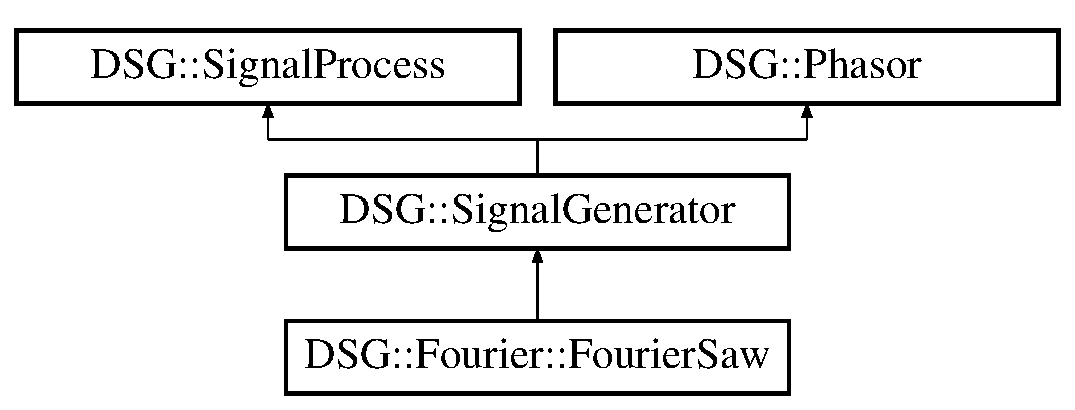
\includegraphics[height=3.000000cm]{class_d_s_g_1_1_fourier_1_1_fourier_saw}
\end{center}
\end{figure}
\subsection*{Public Member Functions}
\begin{DoxyCompactItemize}
\item 
\hyperlink{class_d_s_g_1_1_fourier_1_1_fourier_saw_acfef03c4384ef656110c51102e346c49}{Fourier\+Saw} ()
\item 
\hyperlink{class_d_s_g_1_1_fourier_1_1_fourier_saw_a6062c388900f32e1cfd6df95b9760065}{Fourier\+Saw} (\hyperlink{namespace_d_s_g_a4315a061386fa1014fda09b15d3a6973}{D\+S\+G\+::\+D\+S\+G\+Frequency} const \&frequency, \hyperlink{namespace_d_s_g_a44431ce1eb0a7300efdd207bc879e52c}{D\+S\+G\+::\+D\+S\+G\+Phase} const \&offset)
\item 
virtual \hyperlink{class_d_s_g_1_1_fourier_1_1_fourier_saw_acd28c4942553271ed9f39e8f05b8db6d}{$\sim$\+Fourier\+Saw} ()
\item 
virtual bool \hyperlink{class_d_s_g_1_1_fourier_1_1_fourier_saw_a33061612ff24180f12e9a2c29dfaa116}{Perform} (\hyperlink{namespace_d_s_g_ac39a94cd27ebcd9c1e7502d0c624894a}{D\+S\+G\+::\+D\+S\+G\+Sample} \&signal)
\item 
virtual bool \hyperlink{class_d_s_g_1_1_fourier_1_1_fourier_saw_ac890d9f0af523b63b96b07e6696a32b7}{Perform} (\hyperlink{class_d_s_g_1_1_ring_buffer}{D\+S\+G\+::\+Ring\+Buffer} \&signal)
\item 
virtual \hyperlink{namespace_d_s_g_a4315a061386fa1014fda09b15d3a6973}{D\+S\+G\+::\+D\+S\+G\+Frequency} const \& \hyperlink{class_d_s_g_1_1_fourier_1_1_fourier_saw_afa3d86f404be3665f10c74fe9286ef10}{Frequency} (\hyperlink{namespace_d_s_g_a4315a061386fa1014fda09b15d3a6973}{D\+S\+G\+::\+D\+S\+G\+Frequency} const \&\hyperlink{class_d_s_g_1_1_fourier_1_1_fourier_saw_a97d69a0c03cfb66b1cf6e13fe7073c12}{value})
\end{DoxyCompactItemize}
\subsection*{Protected Attributes}
\begin{DoxyCompactItemize}
\item 
unsigned long \hyperlink{class_d_s_g_1_1_fourier_1_1_fourier_saw_a78d30240b7eb99fcb249b5aafe3d55b2}{\+\_\+h}
\item 
const double \hyperlink{class_d_s_g_1_1_fourier_1_1_fourier_saw_a54895160b61b8d84dc967e7815d07869}{\+\_\+a}
\item 
double \hyperlink{class_d_s_g_1_1_fourier_1_1_fourier_saw_a5df3e5b00224924e106ffdc1d0b6a3cc}{phs}
\item 
double \hyperlink{class_d_s_g_1_1_fourier_1_1_fourier_saw_a97d69a0c03cfb66b1cf6e13fe7073c12}{value}
\item 
int \hyperlink{class_d_s_g_1_1_fourier_1_1_fourier_saw_a261b19d0082558b6e1bb128d267c400d}{i}
\end{DoxyCompactItemize}
\subsection*{Additional Inherited Members}


\subsection{Detailed Description}
\hyperlink{class_d_s_g_1_1_fourier_1_1_fourier_saw}{D\+S\+G\+::\+Fourier\+::\+Fourier\+Saw} -\/ \hyperlink{namespace_d_s_g_1_1_fourier}{Fourier} Series Sawtooth Wave Generator. 

Definition at line \hyperlink{_fourier_saw_8h_source_l00018}{18} of file \hyperlink{_fourier_saw_8h_source}{Fourier\+Saw.\+h}.



\subsection{Constructor \& Destructor Documentation}
\hypertarget{class_d_s_g_1_1_fourier_1_1_fourier_saw_acfef03c4384ef656110c51102e346c49}{\index{D\+S\+G\+::\+Fourier\+::\+Fourier\+Saw@{D\+S\+G\+::\+Fourier\+::\+Fourier\+Saw}!Fourier\+Saw@{Fourier\+Saw}}
\index{Fourier\+Saw@{Fourier\+Saw}!D\+S\+G\+::\+Fourier\+::\+Fourier\+Saw@{D\+S\+G\+::\+Fourier\+::\+Fourier\+Saw}}
\subsubsection[{Fourier\+Saw}]{\setlength{\rightskip}{0pt plus 5cm}D\+S\+G\+::\+Fourier\+::\+Fourier\+Saw\+::\+Fourier\+Saw (
\begin{DoxyParamCaption}
{}
\end{DoxyParamCaption}
)}}\label{class_d_s_g_1_1_fourier_1_1_fourier_saw_acfef03c4384ef656110c51102e346c49}


Definition at line \hyperlink{_fourier_saw_8cpp_source_l00009}{9} of file \hyperlink{_fourier_saw_8cpp_source}{Fourier\+Saw.\+cpp}.


\begin{DoxyCode}
00009 :\hyperlink{class_d_s_g_1_1_signal_generator}{DSG::SignalGenerator}(),\hyperlink{class_d_s_g_1_1_fourier_1_1_fourier_saw_a54895160b61b8d84dc967e7815d07869}{\_a}(1.7/\hyperlink{_p_i_8h_a598a3330b3c21701223ee0ca14316eca}{PI}),\hyperlink{class_d_s_g_1_1_fourier_1_1_fourier_saw_a5df3e5b00224924e106ffdc1d0b6a3cc}{phs}(0),\hyperlink{class_d_s_g_1_1_fourier_1_1_fourier_saw_a97d69a0c03cfb66b1cf6e13fe7073c12}{value}(0),
      \hyperlink{class_d_s_g_1_1_fourier_1_1_fourier_saw_a261b19d0082558b6e1bb128d267c400d}{i}(0)\{\}
\end{DoxyCode}
\hypertarget{class_d_s_g_1_1_fourier_1_1_fourier_saw_a6062c388900f32e1cfd6df95b9760065}{\index{D\+S\+G\+::\+Fourier\+::\+Fourier\+Saw@{D\+S\+G\+::\+Fourier\+::\+Fourier\+Saw}!Fourier\+Saw@{Fourier\+Saw}}
\index{Fourier\+Saw@{Fourier\+Saw}!D\+S\+G\+::\+Fourier\+::\+Fourier\+Saw@{D\+S\+G\+::\+Fourier\+::\+Fourier\+Saw}}
\subsubsection[{Fourier\+Saw}]{\setlength{\rightskip}{0pt plus 5cm}D\+S\+G\+::\+Fourier\+::\+Fourier\+Saw\+::\+Fourier\+Saw (
\begin{DoxyParamCaption}
\item[{{\bf D\+S\+G\+::\+D\+S\+G\+Frequency} const \&}]{frequency, }
\item[{{\bf D\+S\+G\+::\+D\+S\+G\+Phase} const \&}]{offset}
\end{DoxyParamCaption}
)}}\label{class_d_s_g_1_1_fourier_1_1_fourier_saw_a6062c388900f32e1cfd6df95b9760065}


Definition at line \hyperlink{_fourier_saw_8cpp_source_l00010}{10} of file \hyperlink{_fourier_saw_8cpp_source}{Fourier\+Saw.\+cpp}.


\begin{DoxyCode}
00010                                                                                           :
      \hyperlink{class_d_s_g_1_1_signal_generator}{DSG::SignalGenerator}(frequency,offset),\hyperlink{class_d_s_g_1_1_fourier_1_1_fourier_saw_a54895160b61b8d84dc967e7815d07869}{\_a}(1.7/\hyperlink{_p_i_8h_a598a3330b3c21701223ee0ca14316eca}{PI}),\hyperlink{class_d_s_g_1_1_fourier_1_1_fourier_saw_a5df3e5b00224924e106ffdc1d0b6a3cc}{phs}(0),
      \hyperlink{class_d_s_g_1_1_fourier_1_1_fourier_saw_a97d69a0c03cfb66b1cf6e13fe7073c12}{value}(0),\hyperlink{class_d_s_g_1_1_fourier_1_1_fourier_saw_a261b19d0082558b6e1bb128d267c400d}{i}(0)\{
00011     \hyperlink{class_d_s_g_1_1_fourier_1_1_fourier_saw_a78d30240b7eb99fcb249b5aafe3d55b2}{\_h} = \hyperlink{namespace_d_s_g_ab5c4eea42ea10b69cfc32afb83ff1d0d}{MaxHarms}(\hyperlink{class_d_s_g_1_1_signal_generator_a335e7ef058848eca368be51d8544d143}{\_frequency})+1;
00012 \}
\end{DoxyCode}
\hypertarget{class_d_s_g_1_1_fourier_1_1_fourier_saw_acd28c4942553271ed9f39e8f05b8db6d}{\index{D\+S\+G\+::\+Fourier\+::\+Fourier\+Saw@{D\+S\+G\+::\+Fourier\+::\+Fourier\+Saw}!````~Fourier\+Saw@{$\sim$\+Fourier\+Saw}}
\index{````~Fourier\+Saw@{$\sim$\+Fourier\+Saw}!D\+S\+G\+::\+Fourier\+::\+Fourier\+Saw@{D\+S\+G\+::\+Fourier\+::\+Fourier\+Saw}}
\subsubsection[{$\sim$\+Fourier\+Saw}]{\setlength{\rightskip}{0pt plus 5cm}D\+S\+G\+::\+Fourier\+::\+Fourier\+Saw\+::$\sim$\+Fourier\+Saw (
\begin{DoxyParamCaption}
{}
\end{DoxyParamCaption}
)\hspace{0.3cm}{\ttfamily [virtual]}}}\label{class_d_s_g_1_1_fourier_1_1_fourier_saw_acd28c4942553271ed9f39e8f05b8db6d}


Definition at line \hyperlink{_fourier_saw_8cpp_source_l00013}{13} of file \hyperlink{_fourier_saw_8cpp_source}{Fourier\+Saw.\+cpp}.


\begin{DoxyCode}
00013 \{\}\end{DoxyCode}


\subsection{Member Function Documentation}
\hypertarget{class_d_s_g_1_1_fourier_1_1_fourier_saw_afa3d86f404be3665f10c74fe9286ef10}{\index{D\+S\+G\+::\+Fourier\+::\+Fourier\+Saw@{D\+S\+G\+::\+Fourier\+::\+Fourier\+Saw}!Frequency@{Frequency}}
\index{Frequency@{Frequency}!D\+S\+G\+::\+Fourier\+::\+Fourier\+Saw@{D\+S\+G\+::\+Fourier\+::\+Fourier\+Saw}}
\subsubsection[{Frequency}]{\setlength{\rightskip}{0pt plus 5cm}{\bf D\+S\+G\+::\+D\+S\+G\+Frequency} const \& D\+S\+G\+::\+Fourier\+::\+Fourier\+Saw\+::\+Frequency (
\begin{DoxyParamCaption}
\item[{{\bf D\+S\+G\+::\+D\+S\+G\+Frequency} const \&}]{value}
\end{DoxyParamCaption}
)\hspace{0.3cm}{\ttfamily [inline]}, {\ttfamily [virtual]}}}\label{class_d_s_g_1_1_fourier_1_1_fourier_saw_afa3d86f404be3665f10c74fe9286ef10}


Reimplemented from \hyperlink{class_d_s_g_1_1_signal_generator_a30a79888f209d692df3d38f53fc58dfe}{D\+S\+G\+::\+Signal\+Generator}.



Definition at line \hyperlink{_fourier_saw_8h_source_l00053}{53} of file \hyperlink{_fourier_saw_8h_source}{Fourier\+Saw.\+h}.


\begin{DoxyCode}
00053                                                                                                  \{
00054             \hyperlink{class_d_s_g_1_1_signal_generator_a335e7ef058848eca368be51d8544d143}{\_frequency} = \hyperlink{class_d_s_g_1_1_fourier_1_1_fourier_saw_a97d69a0c03cfb66b1cf6e13fe7073c12}{value};
00055             \hyperlink{class_d_s_g_1_1_signal_generator_a01c046bb52bbb74afd789fdce7978f65}{\_dt} = \hyperlink{class_d_s_g_1_1_signal_generator_a335e7ef058848eca368be51d8544d143}{\_frequency}/\hyperlink{namespace_d_s_g_a72df05177db0412c3590070923f62819}{DSG::SampleRate}();
00056             \hyperlink{class_d_s_g_1_1_fourier_1_1_fourier_saw_a78d30240b7eb99fcb249b5aafe3d55b2}{\_h} = \hyperlink{namespace_d_s_g_ab5c4eea42ea10b69cfc32afb83ff1d0d}{MaxHarms}(\hyperlink{class_d_s_g_1_1_signal_generator_a335e7ef058848eca368be51d8544d143}{\_frequency});
00057             \textcolor{keywordflow}{return} \hyperlink{class_d_s_g_1_1_signal_generator_a335e7ef058848eca368be51d8544d143}{\_frequency};
00058         \}
\end{DoxyCode}
\hypertarget{class_d_s_g_1_1_fourier_1_1_fourier_saw_a33061612ff24180f12e9a2c29dfaa116}{\index{D\+S\+G\+::\+Fourier\+::\+Fourier\+Saw@{D\+S\+G\+::\+Fourier\+::\+Fourier\+Saw}!Perform@{Perform}}
\index{Perform@{Perform}!D\+S\+G\+::\+Fourier\+::\+Fourier\+Saw@{D\+S\+G\+::\+Fourier\+::\+Fourier\+Saw}}
\subsubsection[{Perform}]{\setlength{\rightskip}{0pt plus 5cm}bool D\+S\+G\+::\+Fourier\+::\+Fourier\+Saw\+::\+Perform (
\begin{DoxyParamCaption}
\item[{{\bf D\+S\+G\+::\+D\+S\+G\+Sample} \&}]{signal}
\end{DoxyParamCaption}
)\hspace{0.3cm}{\ttfamily [inline]}, {\ttfamily [virtual]}}}\label{class_d_s_g_1_1_fourier_1_1_fourier_saw_a33061612ff24180f12e9a2c29dfaa116}


Reimplemented from \hyperlink{class_d_s_g_1_1_signal_generator_a46fe75a81a242e191c5049d33ddf4155}{D\+S\+G\+::\+Signal\+Generator}.



Definition at line \hyperlink{_fourier_saw_8h_source_l00033}{33} of file \hyperlink{_fourier_saw_8h_source}{Fourier\+Saw.\+h}.


\begin{DoxyCode}
00033                                                                      \{
00034             \textcolor{comment}{//\_h Sine Calls Per Sample where \_h  is theoretically nyquist / frequency}
00035             \hyperlink{class_d_s_g_1_1_fourier_1_1_fourier_saw_a97d69a0c03cfb66b1cf6e13fe7073c12}{value}=\hyperlink{namespace_d_s_g_aad63d316081c7d13a551acf346ee2749}{DSG::Sin}(\hyperlink{class_d_s_g_1_1_signal_generator_a1e23eb94e204b11db75fca030b951065}{\_phasor});
00036             \textcolor{keywordflow}{for} (\hyperlink{class_d_s_g_1_1_fourier_1_1_fourier_saw_a261b19d0082558b6e1bb128d267c400d}{i}=2; \hyperlink{class_d_s_g_1_1_fourier_1_1_fourier_saw_a261b19d0082558b6e1bb128d267c400d}{i}<\hyperlink{class_d_s_g_1_1_fourier_1_1_fourier_saw_a78d30240b7eb99fcb249b5aafe3d55b2}{\_h}; ++\hyperlink{class_d_s_g_1_1_fourier_1_1_fourier_saw_a261b19d0082558b6e1bb128d267c400d}{i}) \{
00037                 \hyperlink{class_d_s_g_1_1_fourier_1_1_fourier_saw_a97d69a0c03cfb66b1cf6e13fe7073c12}{value} += (1.0/\hyperlink{class_d_s_g_1_1_fourier_1_1_fourier_saw_a261b19d0082558b6e1bb128d267c400d}{i}) * \hyperlink{namespace_d_s_g_aad63d316081c7d13a551acf346ee2749}{DSG::Sin}(\hyperlink{class_d_s_g_1_1_signal_generator_a1e23eb94e204b11db75fca030b951065}{\_phasor}*\hyperlink{class_d_s_g_1_1_fourier_1_1_fourier_saw_a261b19d0082558b6e1bb128d267c400d}{i});
00038             \}
00039             \hyperlink{class_d_s_g_1_1_fourier_1_1_fourier_saw_a97d69a0c03cfb66b1cf6e13fe7073c12}{value}*=\hyperlink{class_d_s_g_1_1_fourier_1_1_fourier_saw_a54895160b61b8d84dc967e7815d07869}{\_a};
00040             signal = \hyperlink{class_d_s_g_1_1_fourier_1_1_fourier_saw_a97d69a0c03cfb66b1cf6e13fe7073c12}{value};
00041             \hyperlink{class_d_s_g_1_1_signal_generator_a4c034c5b9ef3dc7548839288355643d5}{step}();
00042             \textcolor{keywordflow}{return} \textcolor{keyword}{true};
00043         \}
\end{DoxyCode}
\hypertarget{class_d_s_g_1_1_fourier_1_1_fourier_saw_ac890d9f0af523b63b96b07e6696a32b7}{\index{D\+S\+G\+::\+Fourier\+::\+Fourier\+Saw@{D\+S\+G\+::\+Fourier\+::\+Fourier\+Saw}!Perform@{Perform}}
\index{Perform@{Perform}!D\+S\+G\+::\+Fourier\+::\+Fourier\+Saw@{D\+S\+G\+::\+Fourier\+::\+Fourier\+Saw}}
\subsubsection[{Perform}]{\setlength{\rightskip}{0pt plus 5cm}bool D\+S\+G\+::\+Fourier\+::\+Fourier\+Saw\+::\+Perform (
\begin{DoxyParamCaption}
\item[{{\bf D\+S\+G\+::\+Ring\+Buffer} \&}]{signal}
\end{DoxyParamCaption}
)\hspace{0.3cm}{\ttfamily [inline]}, {\ttfamily [virtual]}}}\label{class_d_s_g_1_1_fourier_1_1_fourier_saw_ac890d9f0af523b63b96b07e6696a32b7}


Reimplemented from \hyperlink{class_d_s_g_1_1_signal_generator_ab050f80e84e6c8b3e354b56930d6a02b}{D\+S\+G\+::\+Signal\+Generator}.



Definition at line \hyperlink{_fourier_saw_8h_source_l00044}{44} of file \hyperlink{_fourier_saw_8h_source}{Fourier\+Saw.\+h}.


\begin{DoxyCode}
00044                                                                       \{
00045             signal.\hyperlink{class_d_s_g_1_1_ring_buffer_ab23c8003d2857809a816068eeb209d60}{Flush}();
00046             \textcolor{keywordflow}{while} (!signal.\hyperlink{class_d_s_g_1_1_ring_buffer_a53ddb04ffcbb5470a8d2b0a3c65b70cb}{Full}()) \{
00047                 \textcolor{keywordflow}{if} (\hyperlink{class_d_s_g_1_1_fourier_1_1_fourier_saw_a33061612ff24180f12e9a2c29dfaa116}{Perform}(\hyperlink{class_d_s_g_1_1_signal_generator_a28a9b47a1aa0783029f11a19ba0363f2}{\_storage})) \{
00048                     \textcolor{keywordflow}{if}(signal.\hyperlink{class_d_s_g_1_1_ring_buffer_aa5dd2caa0a270173251faee40a43d692}{Write}(\hyperlink{class_d_s_g_1_1_signal_generator_a28a9b47a1aa0783029f11a19ba0363f2}{\_storage}))\{
00049                     \}\textcolor{keywordflow}{else} \textcolor{keywordflow}{return} \textcolor{keyword}{false};
00050                 \}\textcolor{keywordflow}{else} \textcolor{keywordflow}{return} \textcolor{keyword}{false};
00051             \}\textcolor{keywordflow}{return} \textcolor{keyword}{true};
00052         \}
\end{DoxyCode}


\subsection{Member Data Documentation}
\hypertarget{class_d_s_g_1_1_fourier_1_1_fourier_saw_a54895160b61b8d84dc967e7815d07869}{\index{D\+S\+G\+::\+Fourier\+::\+Fourier\+Saw@{D\+S\+G\+::\+Fourier\+::\+Fourier\+Saw}!\+\_\+a@{\+\_\+a}}
\index{\+\_\+a@{\+\_\+a}!D\+S\+G\+::\+Fourier\+::\+Fourier\+Saw@{D\+S\+G\+::\+Fourier\+::\+Fourier\+Saw}}
\subsubsection[{\+\_\+a}]{\setlength{\rightskip}{0pt plus 5cm}const double D\+S\+G\+::\+Fourier\+::\+Fourier\+Saw\+::\+\_\+a\hspace{0.3cm}{\ttfamily [protected]}}}\label{class_d_s_g_1_1_fourier_1_1_fourier_saw_a54895160b61b8d84dc967e7815d07869}


Definition at line \hyperlink{_fourier_saw_8h_source_l00028}{28} of file \hyperlink{_fourier_saw_8h_source}{Fourier\+Saw.\+h}.

\hypertarget{class_d_s_g_1_1_fourier_1_1_fourier_saw_a78d30240b7eb99fcb249b5aafe3d55b2}{\index{D\+S\+G\+::\+Fourier\+::\+Fourier\+Saw@{D\+S\+G\+::\+Fourier\+::\+Fourier\+Saw}!\+\_\+h@{\+\_\+h}}
\index{\+\_\+h@{\+\_\+h}!D\+S\+G\+::\+Fourier\+::\+Fourier\+Saw@{D\+S\+G\+::\+Fourier\+::\+Fourier\+Saw}}
\subsubsection[{\+\_\+h}]{\setlength{\rightskip}{0pt plus 5cm}unsigned long D\+S\+G\+::\+Fourier\+::\+Fourier\+Saw\+::\+\_\+h\hspace{0.3cm}{\ttfamily [protected]}}}\label{class_d_s_g_1_1_fourier_1_1_fourier_saw_a78d30240b7eb99fcb249b5aafe3d55b2}


Definition at line \hyperlink{_fourier_saw_8h_source_l00027}{27} of file \hyperlink{_fourier_saw_8h_source}{Fourier\+Saw.\+h}.

\hypertarget{class_d_s_g_1_1_fourier_1_1_fourier_saw_a261b19d0082558b6e1bb128d267c400d}{\index{D\+S\+G\+::\+Fourier\+::\+Fourier\+Saw@{D\+S\+G\+::\+Fourier\+::\+Fourier\+Saw}!i@{i}}
\index{i@{i}!D\+S\+G\+::\+Fourier\+::\+Fourier\+Saw@{D\+S\+G\+::\+Fourier\+::\+Fourier\+Saw}}
\subsubsection[{i}]{\setlength{\rightskip}{0pt plus 5cm}int D\+S\+G\+::\+Fourier\+::\+Fourier\+Saw\+::i\hspace{0.3cm}{\ttfamily [protected]}}}\label{class_d_s_g_1_1_fourier_1_1_fourier_saw_a261b19d0082558b6e1bb128d267c400d}


Definition at line \hyperlink{_fourier_saw_8h_source_l00031}{31} of file \hyperlink{_fourier_saw_8h_source}{Fourier\+Saw.\+h}.

\hypertarget{class_d_s_g_1_1_fourier_1_1_fourier_saw_a5df3e5b00224924e106ffdc1d0b6a3cc}{\index{D\+S\+G\+::\+Fourier\+::\+Fourier\+Saw@{D\+S\+G\+::\+Fourier\+::\+Fourier\+Saw}!phs@{phs}}
\index{phs@{phs}!D\+S\+G\+::\+Fourier\+::\+Fourier\+Saw@{D\+S\+G\+::\+Fourier\+::\+Fourier\+Saw}}
\subsubsection[{phs}]{\setlength{\rightskip}{0pt plus 5cm}double D\+S\+G\+::\+Fourier\+::\+Fourier\+Saw\+::phs\hspace{0.3cm}{\ttfamily [protected]}}}\label{class_d_s_g_1_1_fourier_1_1_fourier_saw_a5df3e5b00224924e106ffdc1d0b6a3cc}


Definition at line \hyperlink{_fourier_saw_8h_source_l00029}{29} of file \hyperlink{_fourier_saw_8h_source}{Fourier\+Saw.\+h}.

\hypertarget{class_d_s_g_1_1_fourier_1_1_fourier_saw_a97d69a0c03cfb66b1cf6e13fe7073c12}{\index{D\+S\+G\+::\+Fourier\+::\+Fourier\+Saw@{D\+S\+G\+::\+Fourier\+::\+Fourier\+Saw}!value@{value}}
\index{value@{value}!D\+S\+G\+::\+Fourier\+::\+Fourier\+Saw@{D\+S\+G\+::\+Fourier\+::\+Fourier\+Saw}}
\subsubsection[{value}]{\setlength{\rightskip}{0pt plus 5cm}double D\+S\+G\+::\+Fourier\+::\+Fourier\+Saw\+::value\hspace{0.3cm}{\ttfamily [protected]}}}\label{class_d_s_g_1_1_fourier_1_1_fourier_saw_a97d69a0c03cfb66b1cf6e13fe7073c12}


Definition at line \hyperlink{_fourier_saw_8h_source_l00030}{30} of file \hyperlink{_fourier_saw_8h_source}{Fourier\+Saw.\+h}.



The documentation for this class was generated from the following files\+:\begin{DoxyCompactItemize}
\item 
/\+Users/alexanderzywicki/\+Documents/\+D\+S\+G/src/\hyperlink{_fourier_saw_8h}{Fourier\+Saw.\+h}\item 
/\+Users/alexanderzywicki/\+Documents/\+D\+S\+G/src/\hyperlink{_fourier_saw_8cpp}{Fourier\+Saw.\+cpp}\end{DoxyCompactItemize}

\hypertarget{class_d_s_g_1_1_fourier_1_1_fourier_series_generator}{\section{D\+S\+G\+:\+:Fourier\+:\+:Fourier\+Series\+Generator Class Reference}
\label{class_d_s_g_1_1_fourier_1_1_fourier_series_generator}\index{D\+S\+G\+::\+Fourier\+::\+Fourier\+Series\+Generator@{D\+S\+G\+::\+Fourier\+::\+Fourier\+Series\+Generator}}
}


\hyperlink{class_d_s_g_1_1_fourier_1_1_fourier_series_generator}{D\+S\+G\+::\+Fourier\+::\+Fourier\+Series\+Generator} -\/ Generates a wave form using a user specified \hyperlink{namespace_d_s_g_1_1_fourier}{Fourier} Series.  




{\ttfamily \#include $<$Fourier\+Series.\+h$>$}

Inheritance diagram for D\+S\+G\+:\+:Fourier\+:\+:Fourier\+Series\+Generator\+:\begin{figure}[H]
\begin{center}
\leavevmode
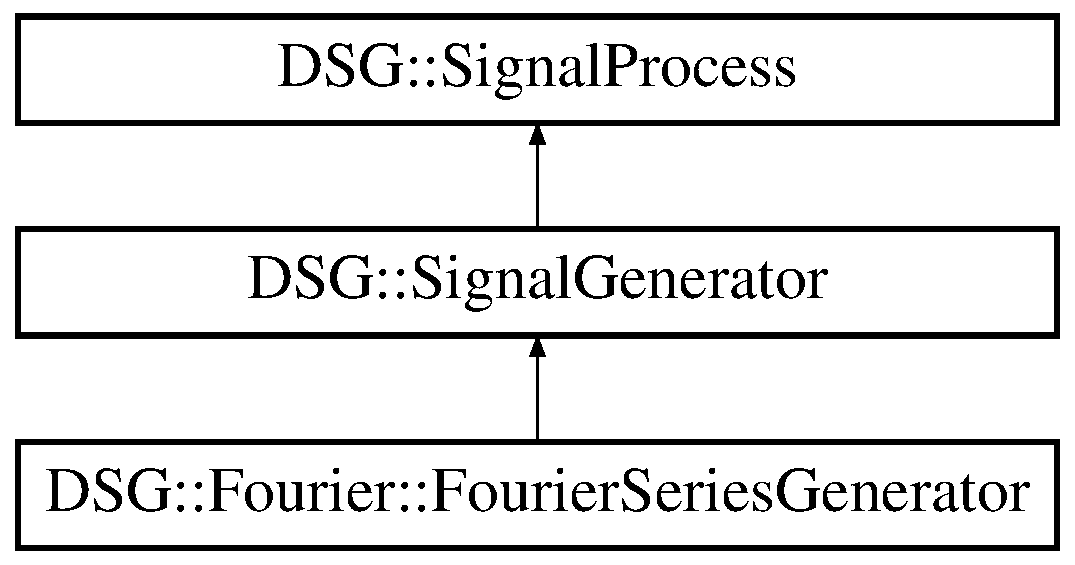
\includegraphics[height=3.000000cm]{class_d_s_g_1_1_fourier_1_1_fourier_series_generator}
\end{center}
\end{figure}
\subsection*{Public Types}
\begin{DoxyCompactItemize}
\item 
typedef std\+::vector$<$ \hyperlink{class_d_s_g_1_1_fourier_1_1_harmonic}{Harmonic} $>$ \hyperlink{class_d_s_g_1_1_fourier_1_1_fourier_series_generator_a32ffe02b67ac07db92ad41e3ee366c94}{Fourier\+Series}
\end{DoxyCompactItemize}
\subsection*{Public Member Functions}
\begin{DoxyCompactItemize}
\item 
\hyperlink{class_d_s_g_1_1_fourier_1_1_fourier_series_generator_a0b73d1fc587d7d22464294b6276c2ec7}{Fourier\+Series\+Generator} ()
\item 
\hyperlink{class_d_s_g_1_1_fourier_1_1_fourier_series_generator_a9227438eb78f40b656ae4f6880fba7d8}{Fourier\+Series\+Generator} (\hyperlink{namespace_d_s_g_a4315a061386fa1014fda09b15d3a6973}{D\+S\+G\+::\+D\+S\+G\+Frequency} const \&frequency, \hyperlink{namespace_d_s_g_a44431ce1eb0a7300efdd207bc879e52c}{D\+S\+G\+::\+D\+S\+G\+Phase} const \&offset)
\item 
virtual \hyperlink{class_d_s_g_1_1_fourier_1_1_fourier_series_generator_a6e5b0a582b040035a47a0855456d71c1}{$\sim$\+Fourier\+Series\+Generator} ()
\item 
virtual bool \hyperlink{class_d_s_g_1_1_fourier_1_1_fourier_series_generator_aa4768d44397b5fab5a30cb86068e161a}{Perform} (\hyperlink{namespace_d_s_g_ac39a94cd27ebcd9c1e7502d0c624894a}{D\+S\+G\+::\+D\+S\+G\+Sample} \&signal)
\item 
virtual bool \hyperlink{class_d_s_g_1_1_fourier_1_1_fourier_series_generator_adce79a239104570f8a6565e708fb70a7}{Perform} (\hyperlink{class_d_s_g_1_1_ring_buffer}{D\+S\+G\+::\+Ring\+Buffer} \&signal)
\item 
void \hyperlink{class_d_s_g_1_1_fourier_1_1_fourier_series_generator_a69b6556f53c7241e37144f5d88381fb7}{Series} (\hyperlink{class_d_s_g_1_1_fourier_1_1_fourier_series_generator_a32ffe02b67ac07db92ad41e3ee366c94}{Fourier\+Series} const \&series)
\item 
\hyperlink{class_d_s_g_1_1_fourier_1_1_fourier_series_generator_a32ffe02b67ac07db92ad41e3ee366c94}{Fourier\+Series} \& \hyperlink{class_d_s_g_1_1_fourier_1_1_fourier_series_generator_a4ed12eb61fe931ceceaeb59a2986a147}{Series} ()
\end{DoxyCompactItemize}
\subsection*{Protected Attributes}
\begin{DoxyCompactItemize}
\item 
\hyperlink{class_d_s_g_1_1_fourier_1_1_fourier_series_generator_a32ffe02b67ac07db92ad41e3ee366c94}{Fourier\+Series} \hyperlink{class_d_s_g_1_1_fourier_1_1_fourier_series_generator_ac66c0907c6daa57f0e33f6b82cc7131d}{\+\_\+series}
\item 
\hyperlink{namespace_d_s_g_ac39a94cd27ebcd9c1e7502d0c624894a}{D\+S\+G\+::\+D\+S\+G\+Sample} \hyperlink{class_d_s_g_1_1_fourier_1_1_fourier_series_generator_a1785e78e21decfc65f650a5e3a435ed8}{value}
\end{DoxyCompactItemize}
\subsection*{Additional Inherited Members}


\subsection{Detailed Description}
\hyperlink{class_d_s_g_1_1_fourier_1_1_fourier_series_generator}{D\+S\+G\+::\+Fourier\+::\+Fourier\+Series\+Generator} -\/ Generates a wave form using a user specified \hyperlink{namespace_d_s_g_1_1_fourier}{Fourier} Series. 

Definition at line \hyperlink{_fourier_series_8h_source_l00032}{32} of file \hyperlink{_fourier_series_8h_source}{Fourier\+Series.\+h}.



\subsection{Member Typedef Documentation}
\hypertarget{class_d_s_g_1_1_fourier_1_1_fourier_series_generator_a32ffe02b67ac07db92ad41e3ee366c94}{\index{D\+S\+G\+::\+Fourier\+::\+Fourier\+Series\+Generator@{D\+S\+G\+::\+Fourier\+::\+Fourier\+Series\+Generator}!Fourier\+Series@{Fourier\+Series}}
\index{Fourier\+Series@{Fourier\+Series}!D\+S\+G\+::\+Fourier\+::\+Fourier\+Series\+Generator@{D\+S\+G\+::\+Fourier\+::\+Fourier\+Series\+Generator}}
\subsubsection[{Fourier\+Series}]{\setlength{\rightskip}{0pt plus 5cm}typedef std\+::vector$<${\bf Harmonic}$>$ {\bf D\+S\+G\+::\+Fourier\+::\+Fourier\+Series\+Generator\+::\+Fourier\+Series}}}\label{class_d_s_g_1_1_fourier_1_1_fourier_series_generator_a32ffe02b67ac07db92ad41e3ee366c94}


Definition at line \hyperlink{_fourier_series_8h_source_l00034}{34} of file \hyperlink{_fourier_series_8h_source}{Fourier\+Series.\+h}.



\subsection{Constructor \& Destructor Documentation}
\hypertarget{class_d_s_g_1_1_fourier_1_1_fourier_series_generator_a0b73d1fc587d7d22464294b6276c2ec7}{\index{D\+S\+G\+::\+Fourier\+::\+Fourier\+Series\+Generator@{D\+S\+G\+::\+Fourier\+::\+Fourier\+Series\+Generator}!Fourier\+Series\+Generator@{Fourier\+Series\+Generator}}
\index{Fourier\+Series\+Generator@{Fourier\+Series\+Generator}!D\+S\+G\+::\+Fourier\+::\+Fourier\+Series\+Generator@{D\+S\+G\+::\+Fourier\+::\+Fourier\+Series\+Generator}}
\subsubsection[{Fourier\+Series\+Generator}]{\setlength{\rightskip}{0pt plus 5cm}D\+S\+G\+::\+Fourier\+::\+Fourier\+Series\+Generator\+::\+Fourier\+Series\+Generator (
\begin{DoxyParamCaption}
{}
\end{DoxyParamCaption}
)}}\label{class_d_s_g_1_1_fourier_1_1_fourier_series_generator_a0b73d1fc587d7d22464294b6276c2ec7}


Definition at line \hyperlink{_fourier_series_8cpp_source_l00029}{29} of file \hyperlink{_fourier_series_8cpp_source}{Fourier\+Series.\+cpp}.


\begin{DoxyCode}
00029 :\hyperlink{class_d_s_g_1_1_signal_generator}{DSG::SignalGenerator}()\{\}
\end{DoxyCode}
\hypertarget{class_d_s_g_1_1_fourier_1_1_fourier_series_generator_a9227438eb78f40b656ae4f6880fba7d8}{\index{D\+S\+G\+::\+Fourier\+::\+Fourier\+Series\+Generator@{D\+S\+G\+::\+Fourier\+::\+Fourier\+Series\+Generator}!Fourier\+Series\+Generator@{Fourier\+Series\+Generator}}
\index{Fourier\+Series\+Generator@{Fourier\+Series\+Generator}!D\+S\+G\+::\+Fourier\+::\+Fourier\+Series\+Generator@{D\+S\+G\+::\+Fourier\+::\+Fourier\+Series\+Generator}}
\subsubsection[{Fourier\+Series\+Generator}]{\setlength{\rightskip}{0pt plus 5cm}D\+S\+G\+::\+Fourier\+::\+Fourier\+Series\+Generator\+::\+Fourier\+Series\+Generator (
\begin{DoxyParamCaption}
\item[{{\bf D\+S\+G\+::\+D\+S\+G\+Frequency} const \&}]{frequency, }
\item[{{\bf D\+S\+G\+::\+D\+S\+G\+Phase} const \&}]{offset}
\end{DoxyParamCaption}
)}}\label{class_d_s_g_1_1_fourier_1_1_fourier_series_generator_a9227438eb78f40b656ae4f6880fba7d8}


Definition at line \hyperlink{_fourier_series_8cpp_source_l00030}{30} of file \hyperlink{_fourier_series_8cpp_source}{Fourier\+Series.\+cpp}.


\begin{DoxyCode}
00030 :\hyperlink{class_d_s_g_1_1_signal_generator}{DSG::SignalGenerator}(frequency,offset)\{\}
\end{DoxyCode}
\hypertarget{class_d_s_g_1_1_fourier_1_1_fourier_series_generator_a6e5b0a582b040035a47a0855456d71c1}{\index{D\+S\+G\+::\+Fourier\+::\+Fourier\+Series\+Generator@{D\+S\+G\+::\+Fourier\+::\+Fourier\+Series\+Generator}!````~Fourier\+Series\+Generator@{$\sim$\+Fourier\+Series\+Generator}}
\index{````~Fourier\+Series\+Generator@{$\sim$\+Fourier\+Series\+Generator}!D\+S\+G\+::\+Fourier\+::\+Fourier\+Series\+Generator@{D\+S\+G\+::\+Fourier\+::\+Fourier\+Series\+Generator}}
\subsubsection[{$\sim$\+Fourier\+Series\+Generator}]{\setlength{\rightskip}{0pt plus 5cm}D\+S\+G\+::\+Fourier\+::\+Fourier\+Series\+Generator\+::$\sim$\+Fourier\+Series\+Generator (
\begin{DoxyParamCaption}
{}
\end{DoxyParamCaption}
)\hspace{0.3cm}{\ttfamily [virtual]}}}\label{class_d_s_g_1_1_fourier_1_1_fourier_series_generator_a6e5b0a582b040035a47a0855456d71c1}


Definition at line \hyperlink{_fourier_series_8cpp_source_l00031}{31} of file \hyperlink{_fourier_series_8cpp_source}{Fourier\+Series.\+cpp}.


\begin{DoxyCode}
00031 \{\}\end{DoxyCode}


\subsection{Member Function Documentation}
\hypertarget{class_d_s_g_1_1_fourier_1_1_fourier_series_generator_aa4768d44397b5fab5a30cb86068e161a}{\index{D\+S\+G\+::\+Fourier\+::\+Fourier\+Series\+Generator@{D\+S\+G\+::\+Fourier\+::\+Fourier\+Series\+Generator}!Perform@{Perform}}
\index{Perform@{Perform}!D\+S\+G\+::\+Fourier\+::\+Fourier\+Series\+Generator@{D\+S\+G\+::\+Fourier\+::\+Fourier\+Series\+Generator}}
\subsubsection[{Perform}]{\setlength{\rightskip}{0pt plus 5cm}bool D\+S\+G\+::\+Fourier\+::\+Fourier\+Series\+Generator\+::\+Perform (
\begin{DoxyParamCaption}
\item[{{\bf D\+S\+G\+::\+D\+S\+G\+Sample} \&}]{signal}
\end{DoxyParamCaption}
)\hspace{0.3cm}{\ttfamily [inline]}, {\ttfamily [virtual]}}}\label{class_d_s_g_1_1_fourier_1_1_fourier_series_generator_aa4768d44397b5fab5a30cb86068e161a}


Reimplemented from \hyperlink{class_d_s_g_1_1_signal_generator_a46fe75a81a242e191c5049d33ddf4155}{D\+S\+G\+::\+Signal\+Generator}.



Definition at line \hyperlink{_fourier_series_8h_source_l00046}{46} of file \hyperlink{_fourier_series_8h_source}{Fourier\+Series.\+h}.


\begin{DoxyCode}
00046                                                                                  \{
00047             \hyperlink{class_d_s_g_1_1_fourier_1_1_fourier_series_generator_a1785e78e21decfc65f650a5e3a435ed8}{value} = \hyperlink{class_d_s_g_1_1_signal_generator_a1e23eb94e204b11db75fca030b951065}{\_phasor};
00048             signal=0;
00049             \textcolor{keywordflow}{for} (\textcolor{keyword}{auto} i = \hyperlink{class_d_s_g_1_1_fourier_1_1_fourier_series_generator_ac66c0907c6daa57f0e33f6b82cc7131d}{\_series}.begin(); i!=\hyperlink{class_d_s_g_1_1_fourier_1_1_fourier_series_generator_ac66c0907c6daa57f0e33f6b82cc7131d}{\_series}.end(); ++i) \{
00050                 signal += \hyperlink{namespace_d_s_g_aad63d316081c7d13a551acf346ee2749}{DSG::Sin}(\hyperlink{class_d_s_g_1_1_signal_generator_a1e23eb94e204b11db75fca030b951065}{\_phasor} * i->Ratio())*i->Amplitude();
00051             \}
00052             \hyperlink{class_d_s_g_1_1_signal_generator_a4c034c5b9ef3dc7548839288355643d5}{step}();
00053             \textcolor{keywordflow}{return} \textcolor{keyword}{true};
00054         \}
\end{DoxyCode}
\hypertarget{class_d_s_g_1_1_fourier_1_1_fourier_series_generator_adce79a239104570f8a6565e708fb70a7}{\index{D\+S\+G\+::\+Fourier\+::\+Fourier\+Series\+Generator@{D\+S\+G\+::\+Fourier\+::\+Fourier\+Series\+Generator}!Perform@{Perform}}
\index{Perform@{Perform}!D\+S\+G\+::\+Fourier\+::\+Fourier\+Series\+Generator@{D\+S\+G\+::\+Fourier\+::\+Fourier\+Series\+Generator}}
\subsubsection[{Perform}]{\setlength{\rightskip}{0pt plus 5cm}bool D\+S\+G\+::\+Fourier\+::\+Fourier\+Series\+Generator\+::\+Perform (
\begin{DoxyParamCaption}
\item[{{\bf D\+S\+G\+::\+Ring\+Buffer} \&}]{signal}
\end{DoxyParamCaption}
)\hspace{0.3cm}{\ttfamily [inline]}, {\ttfamily [virtual]}}}\label{class_d_s_g_1_1_fourier_1_1_fourier_series_generator_adce79a239104570f8a6565e708fb70a7}


Reimplemented from \hyperlink{class_d_s_g_1_1_signal_generator_ab050f80e84e6c8b3e354b56930d6a02b}{D\+S\+G\+::\+Signal\+Generator}.



Definition at line \hyperlink{_fourier_series_8h_source_l00055}{55} of file \hyperlink{_fourier_series_8h_source}{Fourier\+Series.\+h}.


\begin{DoxyCode}
00055                                                                                   \{
00056             signal.\hyperlink{class_d_s_g_1_1_ring_buffer_ab23c8003d2857809a816068eeb209d60}{Flush}();
00057             \textcolor{keywordflow}{while} (!signal.\hyperlink{class_d_s_g_1_1_ring_buffer_a53ddb04ffcbb5470a8d2b0a3c65b70cb}{Full}()) \{
00058                 \textcolor{keywordflow}{if} (\hyperlink{class_d_s_g_1_1_fourier_1_1_fourier_series_generator_aa4768d44397b5fab5a30cb86068e161a}{Perform}(\hyperlink{class_d_s_g_1_1_signal_generator_a28a9b47a1aa0783029f11a19ba0363f2}{\_storage})) \{
00059                     \textcolor{keywordflow}{if}(signal.\hyperlink{class_d_s_g_1_1_ring_buffer_aa5dd2caa0a270173251faee40a43d692}{Write}(\hyperlink{class_d_s_g_1_1_signal_generator_a28a9b47a1aa0783029f11a19ba0363f2}{\_storage}))\{
00060                     \}\textcolor{keywordflow}{else} \textcolor{keywordflow}{return} \textcolor{keyword}{false};
00061                 \}\textcolor{keywordflow}{else} \textcolor{keywordflow}{return} \textcolor{keyword}{false};
00062             \}\textcolor{keywordflow}{return} \textcolor{keyword}{true};
00063         \}
\end{DoxyCode}
\hypertarget{class_d_s_g_1_1_fourier_1_1_fourier_series_generator_a69b6556f53c7241e37144f5d88381fb7}{\index{D\+S\+G\+::\+Fourier\+::\+Fourier\+Series\+Generator@{D\+S\+G\+::\+Fourier\+::\+Fourier\+Series\+Generator}!Series@{Series}}
\index{Series@{Series}!D\+S\+G\+::\+Fourier\+::\+Fourier\+Series\+Generator@{D\+S\+G\+::\+Fourier\+::\+Fourier\+Series\+Generator}}
\subsubsection[{Series}]{\setlength{\rightskip}{0pt plus 5cm}void D\+S\+G\+::\+Fourier\+::\+Fourier\+Series\+Generator\+::\+Series (
\begin{DoxyParamCaption}
\item[{{\bf Fourier\+Series} const \&}]{series}
\end{DoxyParamCaption}
)\hspace{0.3cm}{\ttfamily [inline]}}}\label{class_d_s_g_1_1_fourier_1_1_fourier_series_generator_a69b6556f53c7241e37144f5d88381fb7}


Definition at line \hyperlink{_fourier_series_8h_source_l00064}{64} of file \hyperlink{_fourier_series_8h_source}{Fourier\+Series.\+h}.


\begin{DoxyCode}
00064                                                                                                            
                  \{
00065             \hyperlink{class_d_s_g_1_1_fourier_1_1_fourier_series_generator_ac66c0907c6daa57f0e33f6b82cc7131d}{\_series} = series;
00066         \}
\end{DoxyCode}
\hypertarget{class_d_s_g_1_1_fourier_1_1_fourier_series_generator_a4ed12eb61fe931ceceaeb59a2986a147}{\index{D\+S\+G\+::\+Fourier\+::\+Fourier\+Series\+Generator@{D\+S\+G\+::\+Fourier\+::\+Fourier\+Series\+Generator}!Series@{Series}}
\index{Series@{Series}!D\+S\+G\+::\+Fourier\+::\+Fourier\+Series\+Generator@{D\+S\+G\+::\+Fourier\+::\+Fourier\+Series\+Generator}}
\subsubsection[{Series}]{\setlength{\rightskip}{0pt plus 5cm}{\bf D\+S\+G\+::\+Fourier\+::\+Fourier\+Series\+Generator\+::\+Fourier\+Series} \& D\+S\+G\+::\+Fourier\+::\+Fourier\+Series\+Generator\+::\+Series (
\begin{DoxyParamCaption}
{}
\end{DoxyParamCaption}
)\hspace{0.3cm}{\ttfamily [inline]}}}\label{class_d_s_g_1_1_fourier_1_1_fourier_series_generator_a4ed12eb61fe931ceceaeb59a2986a147}


Definition at line \hyperlink{_fourier_series_8h_source_l00067}{67} of file \hyperlink{_fourier_series_8h_source}{Fourier\+Series.\+h}.


\begin{DoxyCode}
00067                                                                                                       \{
00068             \textcolor{keywordflow}{return} \hyperlink{class_d_s_g_1_1_fourier_1_1_fourier_series_generator_ac66c0907c6daa57f0e33f6b82cc7131d}{\_series};
00069         \}
\end{DoxyCode}


\subsection{Member Data Documentation}
\hypertarget{class_d_s_g_1_1_fourier_1_1_fourier_series_generator_ac66c0907c6daa57f0e33f6b82cc7131d}{\index{D\+S\+G\+::\+Fourier\+::\+Fourier\+Series\+Generator@{D\+S\+G\+::\+Fourier\+::\+Fourier\+Series\+Generator}!\+\_\+series@{\+\_\+series}}
\index{\+\_\+series@{\+\_\+series}!D\+S\+G\+::\+Fourier\+::\+Fourier\+Series\+Generator@{D\+S\+G\+::\+Fourier\+::\+Fourier\+Series\+Generator}}
\subsubsection[{\+\_\+series}]{\setlength{\rightskip}{0pt plus 5cm}{\bf Fourier\+Series} D\+S\+G\+::\+Fourier\+::\+Fourier\+Series\+Generator\+::\+\_\+series\hspace{0.3cm}{\ttfamily [protected]}}}\label{class_d_s_g_1_1_fourier_1_1_fourier_series_generator_ac66c0907c6daa57f0e33f6b82cc7131d}


Definition at line \hyperlink{_fourier_series_8h_source_l00043}{43} of file \hyperlink{_fourier_series_8h_source}{Fourier\+Series.\+h}.

\hypertarget{class_d_s_g_1_1_fourier_1_1_fourier_series_generator_a1785e78e21decfc65f650a5e3a435ed8}{\index{D\+S\+G\+::\+Fourier\+::\+Fourier\+Series\+Generator@{D\+S\+G\+::\+Fourier\+::\+Fourier\+Series\+Generator}!value@{value}}
\index{value@{value}!D\+S\+G\+::\+Fourier\+::\+Fourier\+Series\+Generator@{D\+S\+G\+::\+Fourier\+::\+Fourier\+Series\+Generator}}
\subsubsection[{value}]{\setlength{\rightskip}{0pt plus 5cm}{\bf D\+S\+G\+::\+D\+S\+G\+Sample} D\+S\+G\+::\+Fourier\+::\+Fourier\+Series\+Generator\+::value\hspace{0.3cm}{\ttfamily [protected]}}}\label{class_d_s_g_1_1_fourier_1_1_fourier_series_generator_a1785e78e21decfc65f650a5e3a435ed8}


Definition at line \hyperlink{_fourier_series_8h_source_l00044}{44} of file \hyperlink{_fourier_series_8h_source}{Fourier\+Series.\+h}.



The documentation for this class was generated from the following files\+:\begin{DoxyCompactItemize}
\item 
/\+Users/alexanderzywicki/\+Documents/\+D\+S\+G/src/\hyperlink{_fourier_series_8h}{Fourier\+Series.\+h}\item 
/\+Users/alexanderzywicki/\+Documents/\+D\+S\+G/src/\hyperlink{_fourier_series_8cpp}{Fourier\+Series.\+cpp}\end{DoxyCompactItemize}

\hypertarget{class_d_s_g_1_1_fourier_1_1_fourier_square}{\section{D\+S\+G\+:\+:Fourier\+:\+:Fourier\+Square Class Reference}
\label{class_d_s_g_1_1_fourier_1_1_fourier_square}\index{D\+S\+G\+::\+Fourier\+::\+Fourier\+Square@{D\+S\+G\+::\+Fourier\+::\+Fourier\+Square}}
}


\hyperlink{class_d_s_g_1_1_fourier_1_1_fourier_square}{D\+S\+G\+::\+Fourier\+::\+Fourier\+Square} -\/ \hyperlink{namespace_d_s_g_1_1_fourier}{Fourier} Series Square Wave Generator.  




{\ttfamily \#include $<$Fourier\+Square.\+h$>$}

Inheritance diagram for D\+S\+G\+:\+:Fourier\+:\+:Fourier\+Square\+:\begin{figure}[H]
\begin{center}
\leavevmode
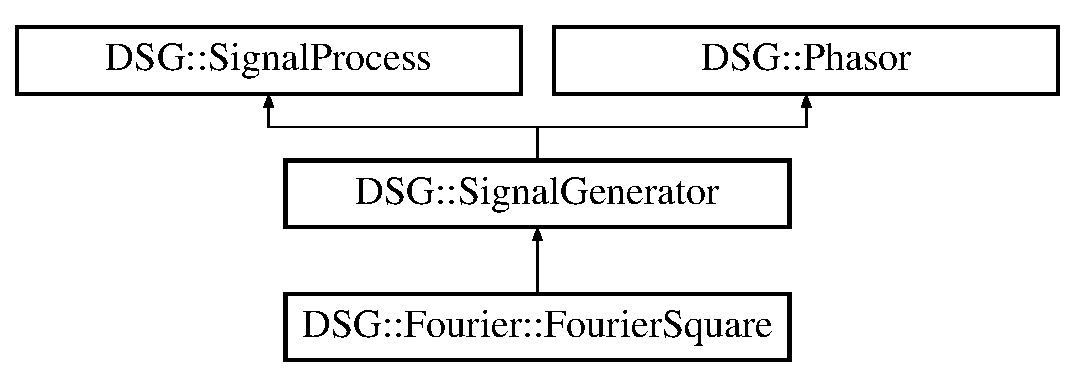
\includegraphics[height=3.000000cm]{class_d_s_g_1_1_fourier_1_1_fourier_square}
\end{center}
\end{figure}
\subsection*{Public Member Functions}
\begin{DoxyCompactItemize}
\item 
\hyperlink{class_d_s_g_1_1_fourier_1_1_fourier_square_a48fa53b8b5ea77013e1bbb2b2467d15e}{Fourier\+Square} ()
\item 
\hyperlink{class_d_s_g_1_1_fourier_1_1_fourier_square_a277316295ca15354a6e507a71cb5f0db}{Fourier\+Square} (\hyperlink{namespace_d_s_g_a4315a061386fa1014fda09b15d3a6973}{D\+S\+G\+::\+D\+S\+G\+Frequency} const \&frequency, \hyperlink{namespace_d_s_g_a44431ce1eb0a7300efdd207bc879e52c}{D\+S\+G\+::\+D\+S\+G\+Phase} const \&offset)
\item 
virtual \hyperlink{class_d_s_g_1_1_fourier_1_1_fourier_square_af78565a799ebfd4be03cc0294dff1f85}{$\sim$\+Fourier\+Square} ()
\item 
virtual bool \hyperlink{class_d_s_g_1_1_fourier_1_1_fourier_square_a05bd0cd3e76ca22e1cede5afb47fbbc4}{Perform} (\hyperlink{namespace_d_s_g_ac39a94cd27ebcd9c1e7502d0c624894a}{D\+S\+G\+::\+D\+S\+G\+Sample} \&signal)
\item 
virtual bool \hyperlink{class_d_s_g_1_1_fourier_1_1_fourier_square_a46028a3615f26876f9c613f983141362}{Perform} (\hyperlink{class_d_s_g_1_1_ring_buffer}{D\+S\+G\+::\+Ring\+Buffer} \&signal)
\item 
virtual \hyperlink{namespace_d_s_g_a4315a061386fa1014fda09b15d3a6973}{D\+S\+G\+::\+D\+S\+G\+Frequency} const \& \hyperlink{class_d_s_g_1_1_fourier_1_1_fourier_square_a120cbb563a518c9412190eaa36cb269f}{Frequency} (\hyperlink{namespace_d_s_g_a4315a061386fa1014fda09b15d3a6973}{D\+S\+G\+::\+D\+S\+G\+Frequency} const \&\hyperlink{class_d_s_g_1_1_fourier_1_1_fourier_square_a5817c7b9b793af6a76278065a67acd9c}{value})
\end{DoxyCompactItemize}
\subsection*{Protected Attributes}
\begin{DoxyCompactItemize}
\item 
unsigned long \hyperlink{class_d_s_g_1_1_fourier_1_1_fourier_square_ac482ccc644bac01f3491503a755b453c}{\+\_\+h}
\item 
const double \hyperlink{class_d_s_g_1_1_fourier_1_1_fourier_square_a974287b077bd7bff2b028dd1af75e3d0}{\+\_\+a}
\item 
double \hyperlink{class_d_s_g_1_1_fourier_1_1_fourier_square_a6e20ab344501c18d79d594ec83f34164}{phs}
\item 
double \hyperlink{class_d_s_g_1_1_fourier_1_1_fourier_square_a5817c7b9b793af6a76278065a67acd9c}{value}
\item 
int \hyperlink{class_d_s_g_1_1_fourier_1_1_fourier_square_ad52c23216a09d1933e5b3289f2d54db2}{i}
\end{DoxyCompactItemize}
\subsection*{Additional Inherited Members}


\subsection{Detailed Description}
\hyperlink{class_d_s_g_1_1_fourier_1_1_fourier_square}{D\+S\+G\+::\+Fourier\+::\+Fourier\+Square} -\/ \hyperlink{namespace_d_s_g_1_1_fourier}{Fourier} Series Square Wave Generator. 

Definition at line \hyperlink{_fourier_square_8h_source_l00034}{34} of file \hyperlink{_fourier_square_8h_source}{Fourier\+Square.\+h}.



\subsection{Constructor \& Destructor Documentation}
\hypertarget{class_d_s_g_1_1_fourier_1_1_fourier_square_a48fa53b8b5ea77013e1bbb2b2467d15e}{\index{D\+S\+G\+::\+Fourier\+::\+Fourier\+Square@{D\+S\+G\+::\+Fourier\+::\+Fourier\+Square}!Fourier\+Square@{Fourier\+Square}}
\index{Fourier\+Square@{Fourier\+Square}!D\+S\+G\+::\+Fourier\+::\+Fourier\+Square@{D\+S\+G\+::\+Fourier\+::\+Fourier\+Square}}
\subsubsection[{Fourier\+Square}]{\setlength{\rightskip}{0pt plus 5cm}D\+S\+G\+::\+Fourier\+::\+Fourier\+Square\+::\+Fourier\+Square (
\begin{DoxyParamCaption}
{}
\end{DoxyParamCaption}
)}}\label{class_d_s_g_1_1_fourier_1_1_fourier_square_a48fa53b8b5ea77013e1bbb2b2467d15e}


Definition at line \hyperlink{_fourier_square_8cpp_source_l00025}{25} of file \hyperlink{_fourier_square_8cpp_source}{Fourier\+Square.\+cpp}.


\begin{DoxyCode}
00025 :\hyperlink{class_d_s_g_1_1_signal_generator}{DSG::SignalGenerator}(),\hyperlink{class_d_s_g_1_1_fourier_1_1_fourier_square_a974287b077bd7bff2b028dd1af75e3d0}{\_a}(3.6/\hyperlink{_p_i_8h_a598a3330b3c21701223ee0ca14316eca}{PI}),\hyperlink{class_d_s_g_1_1_fourier_1_1_fourier_square_a6e20ab344501c18d79d594ec83f34164}{phs}(0),\hyperlink{class_d_s_g_1_1_fourier_1_1_fourier_square_a5817c7b9b793af6a76278065a67acd9c}{value}(0),
      \hyperlink{class_d_s_g_1_1_fourier_1_1_fourier_square_ad52c23216a09d1933e5b3289f2d54db2}{i}(0)\{\}
\end{DoxyCode}
\hypertarget{class_d_s_g_1_1_fourier_1_1_fourier_square_a277316295ca15354a6e507a71cb5f0db}{\index{D\+S\+G\+::\+Fourier\+::\+Fourier\+Square@{D\+S\+G\+::\+Fourier\+::\+Fourier\+Square}!Fourier\+Square@{Fourier\+Square}}
\index{Fourier\+Square@{Fourier\+Square}!D\+S\+G\+::\+Fourier\+::\+Fourier\+Square@{D\+S\+G\+::\+Fourier\+::\+Fourier\+Square}}
\subsubsection[{Fourier\+Square}]{\setlength{\rightskip}{0pt plus 5cm}D\+S\+G\+::\+Fourier\+::\+Fourier\+Square\+::\+Fourier\+Square (
\begin{DoxyParamCaption}
\item[{{\bf D\+S\+G\+::\+D\+S\+G\+Frequency} const \&}]{frequency, }
\item[{{\bf D\+S\+G\+::\+D\+S\+G\+Phase} const \&}]{offset}
\end{DoxyParamCaption}
)}}\label{class_d_s_g_1_1_fourier_1_1_fourier_square_a277316295ca15354a6e507a71cb5f0db}


Definition at line \hyperlink{_fourier_square_8cpp_source_l00026}{26} of file \hyperlink{_fourier_square_8cpp_source}{Fourier\+Square.\+cpp}.


\begin{DoxyCode}
00026                                                                                                 :
      \hyperlink{class_d_s_g_1_1_signal_generator}{DSG::SignalGenerator}(frequency,offset),\hyperlink{class_d_s_g_1_1_fourier_1_1_fourier_square_a974287b077bd7bff2b028dd1af75e3d0}{\_a}(3.6/\hyperlink{_p_i_8h_a598a3330b3c21701223ee0ca14316eca}{PI}),\hyperlink{class_d_s_g_1_1_fourier_1_1_fourier_square_a6e20ab344501c18d79d594ec83f34164}{phs}(0),
      \hyperlink{class_d_s_g_1_1_fourier_1_1_fourier_square_a5817c7b9b793af6a76278065a67acd9c}{value}(0),\hyperlink{class_d_s_g_1_1_fourier_1_1_fourier_square_ad52c23216a09d1933e5b3289f2d54db2}{i}(0)\{
00027     \hyperlink{class_d_s_g_1_1_fourier_1_1_fourier_square_ac482ccc644bac01f3491503a755b453c}{\_h} = \hyperlink{namespace_d_s_g_ab5c4eea42ea10b69cfc32afb83ff1d0d}{MaxHarms}(\hyperlink{class_d_s_g_1_1_signal_generator_a335e7ef058848eca368be51d8544d143}{\_frequency})+1;
00028 \}
\end{DoxyCode}
\hypertarget{class_d_s_g_1_1_fourier_1_1_fourier_square_af78565a799ebfd4be03cc0294dff1f85}{\index{D\+S\+G\+::\+Fourier\+::\+Fourier\+Square@{D\+S\+G\+::\+Fourier\+::\+Fourier\+Square}!````~Fourier\+Square@{$\sim$\+Fourier\+Square}}
\index{````~Fourier\+Square@{$\sim$\+Fourier\+Square}!D\+S\+G\+::\+Fourier\+::\+Fourier\+Square@{D\+S\+G\+::\+Fourier\+::\+Fourier\+Square}}
\subsubsection[{$\sim$\+Fourier\+Square}]{\setlength{\rightskip}{0pt plus 5cm}D\+S\+G\+::\+Fourier\+::\+Fourier\+Square\+::$\sim$\+Fourier\+Square (
\begin{DoxyParamCaption}
{}
\end{DoxyParamCaption}
)\hspace{0.3cm}{\ttfamily [virtual]}}}\label{class_d_s_g_1_1_fourier_1_1_fourier_square_af78565a799ebfd4be03cc0294dff1f85}


Definition at line \hyperlink{_fourier_square_8cpp_source_l00029}{29} of file \hyperlink{_fourier_square_8cpp_source}{Fourier\+Square.\+cpp}.


\begin{DoxyCode}
00029 \{\}\end{DoxyCode}


\subsection{Member Function Documentation}
\hypertarget{class_d_s_g_1_1_fourier_1_1_fourier_square_a120cbb563a518c9412190eaa36cb269f}{\index{D\+S\+G\+::\+Fourier\+::\+Fourier\+Square@{D\+S\+G\+::\+Fourier\+::\+Fourier\+Square}!Frequency@{Frequency}}
\index{Frequency@{Frequency}!D\+S\+G\+::\+Fourier\+::\+Fourier\+Square@{D\+S\+G\+::\+Fourier\+::\+Fourier\+Square}}
\subsubsection[{Frequency}]{\setlength{\rightskip}{0pt plus 5cm}{\bf D\+S\+G\+::\+D\+S\+G\+Frequency} const \& D\+S\+G\+::\+Fourier\+::\+Fourier\+Square\+::\+Frequency (
\begin{DoxyParamCaption}
\item[{{\bf D\+S\+G\+::\+D\+S\+G\+Frequency} const \&}]{value}
\end{DoxyParamCaption}
)\hspace{0.3cm}{\ttfamily [inline]}, {\ttfamily [virtual]}}}\label{class_d_s_g_1_1_fourier_1_1_fourier_square_a120cbb563a518c9412190eaa36cb269f}


Reimplemented from \hyperlink{class_d_s_g_1_1_signal_generator_a30a79888f209d692df3d38f53fc58dfe}{D\+S\+G\+::\+Signal\+Generator}.



Definition at line \hyperlink{_fourier_square_8h_source_l00069}{69} of file \hyperlink{_fourier_square_8h_source}{Fourier\+Square.\+h}.


\begin{DoxyCode}
00069                                                                                                     \{
00070             \hyperlink{class_d_s_g_1_1_signal_generator_a335e7ef058848eca368be51d8544d143}{\_frequency} = \hyperlink{class_d_s_g_1_1_fourier_1_1_fourier_square_a5817c7b9b793af6a76278065a67acd9c}{value};
00071             \hyperlink{class_d_s_g_1_1_signal_generator_a01c046bb52bbb74afd789fdce7978f65}{\_dt} = \hyperlink{class_d_s_g_1_1_signal_generator_a335e7ef058848eca368be51d8544d143}{\_frequency}/\hyperlink{namespace_d_s_g_a72df05177db0412c3590070923f62819}{DSG::SampleRate}();
00072             \hyperlink{class_d_s_g_1_1_fourier_1_1_fourier_square_ac482ccc644bac01f3491503a755b453c}{\_h} = \hyperlink{namespace_d_s_g_ab5c4eea42ea10b69cfc32afb83ff1d0d}{MaxHarms}(\hyperlink{class_d_s_g_1_1_signal_generator_a335e7ef058848eca368be51d8544d143}{\_frequency});
00073             \textcolor{keywordflow}{return} \hyperlink{class_d_s_g_1_1_signal_generator_a335e7ef058848eca368be51d8544d143}{\_frequency};
00074         \}
\end{DoxyCode}
\hypertarget{class_d_s_g_1_1_fourier_1_1_fourier_square_a05bd0cd3e76ca22e1cede5afb47fbbc4}{\index{D\+S\+G\+::\+Fourier\+::\+Fourier\+Square@{D\+S\+G\+::\+Fourier\+::\+Fourier\+Square}!Perform@{Perform}}
\index{Perform@{Perform}!D\+S\+G\+::\+Fourier\+::\+Fourier\+Square@{D\+S\+G\+::\+Fourier\+::\+Fourier\+Square}}
\subsubsection[{Perform}]{\setlength{\rightskip}{0pt plus 5cm}bool D\+S\+G\+::\+Fourier\+::\+Fourier\+Square\+::\+Perform (
\begin{DoxyParamCaption}
\item[{{\bf D\+S\+G\+::\+D\+S\+G\+Sample} \&}]{signal}
\end{DoxyParamCaption}
)\hspace{0.3cm}{\ttfamily [inline]}, {\ttfamily [virtual]}}}\label{class_d_s_g_1_1_fourier_1_1_fourier_square_a05bd0cd3e76ca22e1cede5afb47fbbc4}


Reimplemented from \hyperlink{class_d_s_g_1_1_signal_generator_a46fe75a81a242e191c5049d33ddf4155}{D\+S\+G\+::\+Signal\+Generator}.



Definition at line \hyperlink{_fourier_square_8h_source_l00049}{49} of file \hyperlink{_fourier_square_8h_source}{Fourier\+Square.\+h}.


\begin{DoxyCode}
00049                                                                         \{
00050             \textcolor{comment}{//(\_h/2)+1 Sine Calls Per Sample}
00051             \hyperlink{class_d_s_g_1_1_fourier_1_1_fourier_square_a5817c7b9b793af6a76278065a67acd9c}{value}=\hyperlink{namespace_d_s_g_aad63d316081c7d13a551acf346ee2749}{DSG::Sin}(\hyperlink{class_d_s_g_1_1_signal_generator_a1e23eb94e204b11db75fca030b951065}{\_phasor});\textcolor{comment}{//i=1}
00052             \textcolor{keywordflow}{for} (\hyperlink{class_d_s_g_1_1_fourier_1_1_fourier_square_ad52c23216a09d1933e5b3289f2d54db2}{i}=3; \hyperlink{class_d_s_g_1_1_fourier_1_1_fourier_square_ad52c23216a09d1933e5b3289f2d54db2}{i}<\hyperlink{class_d_s_g_1_1_fourier_1_1_fourier_square_ac482ccc644bac01f3491503a755b453c}{\_h}; \hyperlink{class_d_s_g_1_1_fourier_1_1_fourier_square_ad52c23216a09d1933e5b3289f2d54db2}{i}+=2) \{\textcolor{comment}{//i=3..5..7..}
00053                 \hyperlink{class_d_s_g_1_1_fourier_1_1_fourier_square_a5817c7b9b793af6a76278065a67acd9c}{value} += (1.0/\hyperlink{class_d_s_g_1_1_fourier_1_1_fourier_square_ad52c23216a09d1933e5b3289f2d54db2}{i}) * \hyperlink{namespace_d_s_g_aad63d316081c7d13a551acf346ee2749}{DSG::Sin}(\hyperlink{class_d_s_g_1_1_signal_generator_a1e23eb94e204b11db75fca030b951065}{\_phasor}*\hyperlink{class_d_s_g_1_1_fourier_1_1_fourier_square_ad52c23216a09d1933e5b3289f2d54db2}{i});
00054             \}
00055             \hyperlink{class_d_s_g_1_1_fourier_1_1_fourier_square_a5817c7b9b793af6a76278065a67acd9c}{value}*=\hyperlink{class_d_s_g_1_1_fourier_1_1_fourier_square_a974287b077bd7bff2b028dd1af75e3d0}{\_a};
00056             signal = \hyperlink{class_d_s_g_1_1_fourier_1_1_fourier_square_a5817c7b9b793af6a76278065a67acd9c}{value};
00057             \hyperlink{class_d_s_g_1_1_signal_generator_a4c034c5b9ef3dc7548839288355643d5}{step}();
00058             \textcolor{keywordflow}{return} \textcolor{keyword}{true};
00059         \}
\end{DoxyCode}
\hypertarget{class_d_s_g_1_1_fourier_1_1_fourier_square_a46028a3615f26876f9c613f983141362}{\index{D\+S\+G\+::\+Fourier\+::\+Fourier\+Square@{D\+S\+G\+::\+Fourier\+::\+Fourier\+Square}!Perform@{Perform}}
\index{Perform@{Perform}!D\+S\+G\+::\+Fourier\+::\+Fourier\+Square@{D\+S\+G\+::\+Fourier\+::\+Fourier\+Square}}
\subsubsection[{Perform}]{\setlength{\rightskip}{0pt plus 5cm}bool D\+S\+G\+::\+Fourier\+::\+Fourier\+Square\+::\+Perform (
\begin{DoxyParamCaption}
\item[{{\bf D\+S\+G\+::\+Ring\+Buffer} \&}]{signal}
\end{DoxyParamCaption}
)\hspace{0.3cm}{\ttfamily [inline]}, {\ttfamily [virtual]}}}\label{class_d_s_g_1_1_fourier_1_1_fourier_square_a46028a3615f26876f9c613f983141362}


Reimplemented from \hyperlink{class_d_s_g_1_1_signal_generator_ab050f80e84e6c8b3e354b56930d6a02b}{D\+S\+G\+::\+Signal\+Generator}.



Definition at line \hyperlink{_fourier_square_8h_source_l00060}{60} of file \hyperlink{_fourier_square_8h_source}{Fourier\+Square.\+h}.


\begin{DoxyCode}
00060                                                                          \{
00061             signal.\hyperlink{class_d_s_g_1_1_ring_buffer_ab23c8003d2857809a816068eeb209d60}{Flush}();
00062             \textcolor{keywordflow}{while} (!signal.\hyperlink{class_d_s_g_1_1_ring_buffer_a53ddb04ffcbb5470a8d2b0a3c65b70cb}{Full}()) \{
00063                 \textcolor{keywordflow}{if} (\hyperlink{class_d_s_g_1_1_fourier_1_1_fourier_square_a05bd0cd3e76ca22e1cede5afb47fbbc4}{Perform}(\hyperlink{class_d_s_g_1_1_signal_generator_a28a9b47a1aa0783029f11a19ba0363f2}{\_storage})) \{
00064                     \textcolor{keywordflow}{if}(signal.\hyperlink{class_d_s_g_1_1_ring_buffer_aa5dd2caa0a270173251faee40a43d692}{Write}(\hyperlink{class_d_s_g_1_1_signal_generator_a28a9b47a1aa0783029f11a19ba0363f2}{\_storage}))\{
00065                     \}\textcolor{keywordflow}{else} \textcolor{keywordflow}{return} \textcolor{keyword}{false};
00066                 \}\textcolor{keywordflow}{else} \textcolor{keywordflow}{return} \textcolor{keyword}{false};
00067             \}\textcolor{keywordflow}{return} \textcolor{keyword}{true};
00068         \}
\end{DoxyCode}


\subsection{Member Data Documentation}
\hypertarget{class_d_s_g_1_1_fourier_1_1_fourier_square_a974287b077bd7bff2b028dd1af75e3d0}{\index{D\+S\+G\+::\+Fourier\+::\+Fourier\+Square@{D\+S\+G\+::\+Fourier\+::\+Fourier\+Square}!\+\_\+a@{\+\_\+a}}
\index{\+\_\+a@{\+\_\+a}!D\+S\+G\+::\+Fourier\+::\+Fourier\+Square@{D\+S\+G\+::\+Fourier\+::\+Fourier\+Square}}
\subsubsection[{\+\_\+a}]{\setlength{\rightskip}{0pt plus 5cm}const double D\+S\+G\+::\+Fourier\+::\+Fourier\+Square\+::\+\_\+a\hspace{0.3cm}{\ttfamily [protected]}}}\label{class_d_s_g_1_1_fourier_1_1_fourier_square_a974287b077bd7bff2b028dd1af75e3d0}


Definition at line \hyperlink{_fourier_square_8h_source_l00044}{44} of file \hyperlink{_fourier_square_8h_source}{Fourier\+Square.\+h}.

\hypertarget{class_d_s_g_1_1_fourier_1_1_fourier_square_ac482ccc644bac01f3491503a755b453c}{\index{D\+S\+G\+::\+Fourier\+::\+Fourier\+Square@{D\+S\+G\+::\+Fourier\+::\+Fourier\+Square}!\+\_\+h@{\+\_\+h}}
\index{\+\_\+h@{\+\_\+h}!D\+S\+G\+::\+Fourier\+::\+Fourier\+Square@{D\+S\+G\+::\+Fourier\+::\+Fourier\+Square}}
\subsubsection[{\+\_\+h}]{\setlength{\rightskip}{0pt plus 5cm}unsigned long D\+S\+G\+::\+Fourier\+::\+Fourier\+Square\+::\+\_\+h\hspace{0.3cm}{\ttfamily [protected]}}}\label{class_d_s_g_1_1_fourier_1_1_fourier_square_ac482ccc644bac01f3491503a755b453c}


Definition at line \hyperlink{_fourier_square_8h_source_l00043}{43} of file \hyperlink{_fourier_square_8h_source}{Fourier\+Square.\+h}.

\hypertarget{class_d_s_g_1_1_fourier_1_1_fourier_square_ad52c23216a09d1933e5b3289f2d54db2}{\index{D\+S\+G\+::\+Fourier\+::\+Fourier\+Square@{D\+S\+G\+::\+Fourier\+::\+Fourier\+Square}!i@{i}}
\index{i@{i}!D\+S\+G\+::\+Fourier\+::\+Fourier\+Square@{D\+S\+G\+::\+Fourier\+::\+Fourier\+Square}}
\subsubsection[{i}]{\setlength{\rightskip}{0pt plus 5cm}int D\+S\+G\+::\+Fourier\+::\+Fourier\+Square\+::i\hspace{0.3cm}{\ttfamily [protected]}}}\label{class_d_s_g_1_1_fourier_1_1_fourier_square_ad52c23216a09d1933e5b3289f2d54db2}


Definition at line \hyperlink{_fourier_square_8h_source_l00047}{47} of file \hyperlink{_fourier_square_8h_source}{Fourier\+Square.\+h}.

\hypertarget{class_d_s_g_1_1_fourier_1_1_fourier_square_a6e20ab344501c18d79d594ec83f34164}{\index{D\+S\+G\+::\+Fourier\+::\+Fourier\+Square@{D\+S\+G\+::\+Fourier\+::\+Fourier\+Square}!phs@{phs}}
\index{phs@{phs}!D\+S\+G\+::\+Fourier\+::\+Fourier\+Square@{D\+S\+G\+::\+Fourier\+::\+Fourier\+Square}}
\subsubsection[{phs}]{\setlength{\rightskip}{0pt plus 5cm}double D\+S\+G\+::\+Fourier\+::\+Fourier\+Square\+::phs\hspace{0.3cm}{\ttfamily [protected]}}}\label{class_d_s_g_1_1_fourier_1_1_fourier_square_a6e20ab344501c18d79d594ec83f34164}


Definition at line \hyperlink{_fourier_square_8h_source_l00045}{45} of file \hyperlink{_fourier_square_8h_source}{Fourier\+Square.\+h}.

\hypertarget{class_d_s_g_1_1_fourier_1_1_fourier_square_a5817c7b9b793af6a76278065a67acd9c}{\index{D\+S\+G\+::\+Fourier\+::\+Fourier\+Square@{D\+S\+G\+::\+Fourier\+::\+Fourier\+Square}!value@{value}}
\index{value@{value}!D\+S\+G\+::\+Fourier\+::\+Fourier\+Square@{D\+S\+G\+::\+Fourier\+::\+Fourier\+Square}}
\subsubsection[{value}]{\setlength{\rightskip}{0pt plus 5cm}double D\+S\+G\+::\+Fourier\+::\+Fourier\+Square\+::value\hspace{0.3cm}{\ttfamily [protected]}}}\label{class_d_s_g_1_1_fourier_1_1_fourier_square_a5817c7b9b793af6a76278065a67acd9c}


Definition at line \hyperlink{_fourier_square_8h_source_l00046}{46} of file \hyperlink{_fourier_square_8h_source}{Fourier\+Square.\+h}.



The documentation for this class was generated from the following files\+:\begin{DoxyCompactItemize}
\item 
\hyperlink{_fourier_square_8h}{Fourier\+Square.\+h}\item 
\hyperlink{_fourier_square_8cpp}{Fourier\+Square.\+cpp}\end{DoxyCompactItemize}

\hypertarget{class_d_s_g_1_1_fourier_1_1_fourier_triangle}{\section{D\+S\+G\+:\+:Fourier\+:\+:Fourier\+Triangle Class Reference}
\label{class_d_s_g_1_1_fourier_1_1_fourier_triangle}\index{D\+S\+G\+::\+Fourier\+::\+Fourier\+Triangle@{D\+S\+G\+::\+Fourier\+::\+Fourier\+Triangle}}
}


\hyperlink{class_d_s_g_1_1_fourier_1_1_fourier_triangle}{D\+S\+G\+::\+Fourier\+::\+Fourier\+Triangle} -\/ \hyperlink{namespace_d_s_g_1_1_fourier}{Fourier} Series Triangle Wave Generator.  




{\ttfamily \#include $<$Fourier\+Triangle.\+h$>$}

Inheritance diagram for D\+S\+G\+:\+:Fourier\+:\+:Fourier\+Triangle\+:\begin{figure}[H]
\begin{center}
\leavevmode
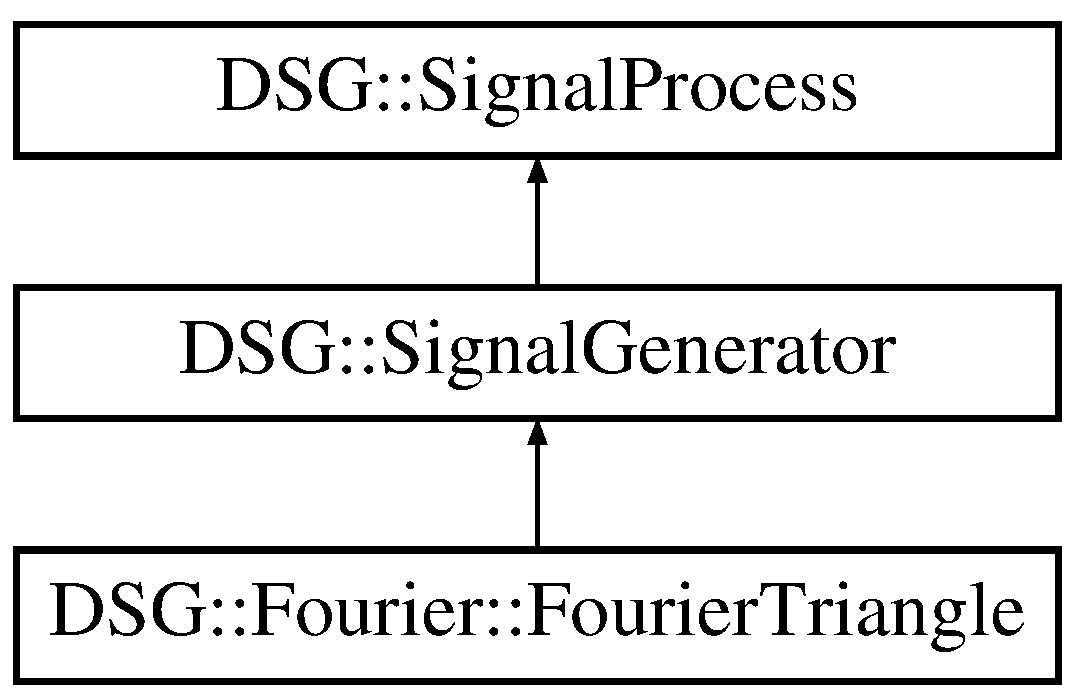
\includegraphics[height=3.000000cm]{class_d_s_g_1_1_fourier_1_1_fourier_triangle}
\end{center}
\end{figure}
\subsection*{Public Member Functions}
\begin{DoxyCompactItemize}
\item 
\hyperlink{class_d_s_g_1_1_fourier_1_1_fourier_triangle_a4129c053eddd87256ae39552a06ce329}{Fourier\+Triangle} ()
\item 
\hyperlink{class_d_s_g_1_1_fourier_1_1_fourier_triangle_abf887c6f5aada92780224511988cb688}{Fourier\+Triangle} (\hyperlink{namespace_d_s_g_a4315a061386fa1014fda09b15d3a6973}{D\+S\+G\+::\+D\+S\+G\+Frequency} const \&frequency, \hyperlink{namespace_d_s_g_a44431ce1eb0a7300efdd207bc879e52c}{D\+S\+G\+::\+D\+S\+G\+Phase} const \&offset)
\item 
virtual \hyperlink{class_d_s_g_1_1_fourier_1_1_fourier_triangle_a780bfb898d144200ff2bfb48849b4d24}{$\sim$\+Fourier\+Triangle} ()
\item 
virtual bool \hyperlink{class_d_s_g_1_1_fourier_1_1_fourier_triangle_ab5b947c1fc1f34a461c863b18e3e877d}{Perform} (\hyperlink{namespace_d_s_g_ac39a94cd27ebcd9c1e7502d0c624894a}{D\+S\+G\+::\+D\+S\+G\+Sample} \&signal)
\item 
virtual bool \hyperlink{class_d_s_g_1_1_fourier_1_1_fourier_triangle_a27b082e69cc7d70223dd3fbc552ba5bc}{Perform} (\hyperlink{class_d_s_g_1_1_ring_buffer}{D\+S\+G\+::\+Ring\+Buffer} \&signal)
\item 
virtual \hyperlink{namespace_d_s_g_a4315a061386fa1014fda09b15d3a6973}{D\+S\+G\+::\+D\+S\+G\+Frequency} const \& \hyperlink{class_d_s_g_1_1_fourier_1_1_fourier_triangle_a278a51ed8af32ea371adc903b9b25039}{Frequency} (\hyperlink{namespace_d_s_g_a4315a061386fa1014fda09b15d3a6973}{D\+S\+G\+::\+D\+S\+G\+Frequency} const \&\hyperlink{class_d_s_g_1_1_fourier_1_1_fourier_triangle_a11216186ce96fc78c7720cad3e01d025}{value})
\end{DoxyCompactItemize}
\subsection*{Protected Attributes}
\begin{DoxyCompactItemize}
\item 
unsigned long \hyperlink{class_d_s_g_1_1_fourier_1_1_fourier_triangle_a6fe21fae0d58d6221602e4bd74c30a80}{\+\_\+h}
\item 
const double \hyperlink{class_d_s_g_1_1_fourier_1_1_fourier_triangle_a64263fc3fa98179d57d34a3f105d8c97}{\+\_\+a}
\item 
double \hyperlink{class_d_s_g_1_1_fourier_1_1_fourier_triangle_a274fb09e2f14f88ec969dcaa7ad423f4}{phs}
\item 
double \hyperlink{class_d_s_g_1_1_fourier_1_1_fourier_triangle_a11216186ce96fc78c7720cad3e01d025}{value}
\item 
int \hyperlink{class_d_s_g_1_1_fourier_1_1_fourier_triangle_a041154af261bce33f4764f60b6606ea4}{i}
\end{DoxyCompactItemize}
\subsection*{Additional Inherited Members}


\subsection{Detailed Description}
\hyperlink{class_d_s_g_1_1_fourier_1_1_fourier_triangle}{D\+S\+G\+::\+Fourier\+::\+Fourier\+Triangle} -\/ \hyperlink{namespace_d_s_g_1_1_fourier}{Fourier} Series Triangle Wave Generator. 

Definition at line \hyperlink{_fourier_triangle_8h_source_l00034}{34} of file \hyperlink{_fourier_triangle_8h_source}{Fourier\+Triangle.\+h}.



\subsection{Constructor \& Destructor Documentation}
\hypertarget{class_d_s_g_1_1_fourier_1_1_fourier_triangle_a4129c053eddd87256ae39552a06ce329}{\index{D\+S\+G\+::\+Fourier\+::\+Fourier\+Triangle@{D\+S\+G\+::\+Fourier\+::\+Fourier\+Triangle}!Fourier\+Triangle@{Fourier\+Triangle}}
\index{Fourier\+Triangle@{Fourier\+Triangle}!D\+S\+G\+::\+Fourier\+::\+Fourier\+Triangle@{D\+S\+G\+::\+Fourier\+::\+Fourier\+Triangle}}
\subsubsection[{Fourier\+Triangle}]{\setlength{\rightskip}{0pt plus 5cm}D\+S\+G\+::\+Fourier\+::\+Fourier\+Triangle\+::\+Fourier\+Triangle (
\begin{DoxyParamCaption}
{}
\end{DoxyParamCaption}
)}}\label{class_d_s_g_1_1_fourier_1_1_fourier_triangle_a4129c053eddd87256ae39552a06ce329}


Definition at line \hyperlink{_fourier_triangle_8cpp_source_l00025}{25} of file \hyperlink{_fourier_triangle_8cpp_source}{Fourier\+Triangle.\+cpp}.


\begin{DoxyCode}
00025 :\hyperlink{class_d_s_g_1_1_signal_generator}{DSG::SignalGenerator}(),\hyperlink{class_d_s_g_1_1_fourier_1_1_fourier_triangle_a64263fc3fa98179d57d34a3f105d8c97}{\_a}(8.0/(\hyperlink{_p_i_8h_a598a3330b3c21701223ee0ca14316eca}{PI}*\hyperlink{_p_i_8h_a598a3330b3c21701223ee0ca14316eca}{PI})),\hyperlink{class_d_s_g_1_1_fourier_1_1_fourier_triangle_a274fb09e2f14f88ec969dcaa7ad423f4}{phs}(0),
      \hyperlink{class_d_s_g_1_1_fourier_1_1_fourier_triangle_a11216186ce96fc78c7720cad3e01d025}{value}(0),\hyperlink{class_d_s_g_1_1_fourier_1_1_fourier_triangle_a041154af261bce33f4764f60b6606ea4}{i}(0)\{\}
\end{DoxyCode}
\hypertarget{class_d_s_g_1_1_fourier_1_1_fourier_triangle_abf887c6f5aada92780224511988cb688}{\index{D\+S\+G\+::\+Fourier\+::\+Fourier\+Triangle@{D\+S\+G\+::\+Fourier\+::\+Fourier\+Triangle}!Fourier\+Triangle@{Fourier\+Triangle}}
\index{Fourier\+Triangle@{Fourier\+Triangle}!D\+S\+G\+::\+Fourier\+::\+Fourier\+Triangle@{D\+S\+G\+::\+Fourier\+::\+Fourier\+Triangle}}
\subsubsection[{Fourier\+Triangle}]{\setlength{\rightskip}{0pt plus 5cm}D\+S\+G\+::\+Fourier\+::\+Fourier\+Triangle\+::\+Fourier\+Triangle (
\begin{DoxyParamCaption}
\item[{{\bf D\+S\+G\+::\+D\+S\+G\+Frequency} const \&}]{frequency, }
\item[{{\bf D\+S\+G\+::\+D\+S\+G\+Phase} const \&}]{offset}
\end{DoxyParamCaption}
)}}\label{class_d_s_g_1_1_fourier_1_1_fourier_triangle_abf887c6f5aada92780224511988cb688}


Definition at line \hyperlink{_fourier_triangle_8cpp_source_l00026}{26} of file \hyperlink{_fourier_triangle_8cpp_source}{Fourier\+Triangle.\+cpp}.


\begin{DoxyCode}
00026                                                                                                     :
      \hyperlink{class_d_s_g_1_1_signal_generator}{DSG::SignalGenerator}(frequency,offset),\hyperlink{class_d_s_g_1_1_fourier_1_1_fourier_triangle_a64263fc3fa98179d57d34a3f105d8c97}{\_a}(8.0/(\hyperlink{_p_i_8h_a598a3330b3c21701223ee0ca14316eca}{PI}*\hyperlink{_p_i_8h_a598a3330b3c21701223ee0ca14316eca}{PI})),
      \hyperlink{class_d_s_g_1_1_fourier_1_1_fourier_triangle_a274fb09e2f14f88ec969dcaa7ad423f4}{phs}(0),\hyperlink{class_d_s_g_1_1_fourier_1_1_fourier_triangle_a11216186ce96fc78c7720cad3e01d025}{value}(0),\hyperlink{class_d_s_g_1_1_fourier_1_1_fourier_triangle_a041154af261bce33f4764f60b6606ea4}{i}(0)\{
00027     \hyperlink{class_d_s_g_1_1_fourier_1_1_fourier_triangle_a6fe21fae0d58d6221602e4bd74c30a80}{\_h} = \hyperlink{namespace_d_s_g_ab5c4eea42ea10b69cfc32afb83ff1d0d}{MaxHarms}(\hyperlink{class_d_s_g_1_1_signal_generator_a335e7ef058848eca368be51d8544d143}{\_frequency})+1;
00028 \}
\end{DoxyCode}
\hypertarget{class_d_s_g_1_1_fourier_1_1_fourier_triangle_a780bfb898d144200ff2bfb48849b4d24}{\index{D\+S\+G\+::\+Fourier\+::\+Fourier\+Triangle@{D\+S\+G\+::\+Fourier\+::\+Fourier\+Triangle}!````~Fourier\+Triangle@{$\sim$\+Fourier\+Triangle}}
\index{````~Fourier\+Triangle@{$\sim$\+Fourier\+Triangle}!D\+S\+G\+::\+Fourier\+::\+Fourier\+Triangle@{D\+S\+G\+::\+Fourier\+::\+Fourier\+Triangle}}
\subsubsection[{$\sim$\+Fourier\+Triangle}]{\setlength{\rightskip}{0pt plus 5cm}D\+S\+G\+::\+Fourier\+::\+Fourier\+Triangle\+::$\sim$\+Fourier\+Triangle (
\begin{DoxyParamCaption}
{}
\end{DoxyParamCaption}
)\hspace{0.3cm}{\ttfamily [virtual]}}}\label{class_d_s_g_1_1_fourier_1_1_fourier_triangle_a780bfb898d144200ff2bfb48849b4d24}


Definition at line \hyperlink{_fourier_triangle_8cpp_source_l00029}{29} of file \hyperlink{_fourier_triangle_8cpp_source}{Fourier\+Triangle.\+cpp}.


\begin{DoxyCode}
00029 \{\}\end{DoxyCode}


\subsection{Member Function Documentation}
\hypertarget{class_d_s_g_1_1_fourier_1_1_fourier_triangle_a278a51ed8af32ea371adc903b9b25039}{\index{D\+S\+G\+::\+Fourier\+::\+Fourier\+Triangle@{D\+S\+G\+::\+Fourier\+::\+Fourier\+Triangle}!Frequency@{Frequency}}
\index{Frequency@{Frequency}!D\+S\+G\+::\+Fourier\+::\+Fourier\+Triangle@{D\+S\+G\+::\+Fourier\+::\+Fourier\+Triangle}}
\subsubsection[{Frequency}]{\setlength{\rightskip}{0pt plus 5cm}{\bf D\+S\+G\+::\+D\+S\+G\+Frequency} const \& D\+S\+G\+::\+Fourier\+::\+Fourier\+Triangle\+::\+Frequency (
\begin{DoxyParamCaption}
\item[{{\bf D\+S\+G\+::\+D\+S\+G\+Frequency} const \&}]{value}
\end{DoxyParamCaption}
)\hspace{0.3cm}{\ttfamily [inline]}, {\ttfamily [virtual]}}}\label{class_d_s_g_1_1_fourier_1_1_fourier_triangle_a278a51ed8af32ea371adc903b9b25039}


Reimplemented from \hyperlink{class_d_s_g_1_1_signal_generator_a30a79888f209d692df3d38f53fc58dfe}{D\+S\+G\+::\+Signal\+Generator}.



Definition at line \hyperlink{_fourier_triangle_8h_source_l00071}{71} of file \hyperlink{_fourier_triangle_8h_source}{Fourier\+Triangle.\+h}.


\begin{DoxyCode}
00071                                                                                                       \{
00072             \hyperlink{class_d_s_g_1_1_signal_generator_a335e7ef058848eca368be51d8544d143}{\_frequency} = \hyperlink{class_d_s_g_1_1_fourier_1_1_fourier_triangle_a11216186ce96fc78c7720cad3e01d025}{value};
00073             \hyperlink{class_d_s_g_1_1_signal_generator_a01c046bb52bbb74afd789fdce7978f65}{\_dt} = \hyperlink{class_d_s_g_1_1_signal_generator_a335e7ef058848eca368be51d8544d143}{\_frequency}/\hyperlink{namespace_d_s_g_a72df05177db0412c3590070923f62819}{DSG::SampleRate}();
00074             \hyperlink{class_d_s_g_1_1_fourier_1_1_fourier_triangle_a6fe21fae0d58d6221602e4bd74c30a80}{\_h} = \hyperlink{namespace_d_s_g_ab5c4eea42ea10b69cfc32afb83ff1d0d}{MaxHarms}(\hyperlink{class_d_s_g_1_1_signal_generator_a335e7ef058848eca368be51d8544d143}{\_frequency});
00075             \textcolor{keywordflow}{return} \hyperlink{class_d_s_g_1_1_signal_generator_a335e7ef058848eca368be51d8544d143}{\_frequency};
00076         \}
\end{DoxyCode}
\hypertarget{class_d_s_g_1_1_fourier_1_1_fourier_triangle_ab5b947c1fc1f34a461c863b18e3e877d}{\index{D\+S\+G\+::\+Fourier\+::\+Fourier\+Triangle@{D\+S\+G\+::\+Fourier\+::\+Fourier\+Triangle}!Perform@{Perform}}
\index{Perform@{Perform}!D\+S\+G\+::\+Fourier\+::\+Fourier\+Triangle@{D\+S\+G\+::\+Fourier\+::\+Fourier\+Triangle}}
\subsubsection[{Perform}]{\setlength{\rightskip}{0pt plus 5cm}bool D\+S\+G\+::\+Fourier\+::\+Fourier\+Triangle\+::\+Perform (
\begin{DoxyParamCaption}
\item[{{\bf D\+S\+G\+::\+D\+S\+G\+Sample} \&}]{signal}
\end{DoxyParamCaption}
)\hspace{0.3cm}{\ttfamily [inline]}, {\ttfamily [virtual]}}}\label{class_d_s_g_1_1_fourier_1_1_fourier_triangle_ab5b947c1fc1f34a461c863b18e3e877d}


Reimplemented from \hyperlink{class_d_s_g_1_1_signal_generator_a46fe75a81a242e191c5049d33ddf4155}{D\+S\+G\+::\+Signal\+Generator}.



Definition at line \hyperlink{_fourier_triangle_8h_source_l00049}{49} of file \hyperlink{_fourier_triangle_8h_source}{Fourier\+Triangle.\+h}.


\begin{DoxyCode}
00049                                                                           \{
00050             \textcolor{comment}{//(\_h/2)+1 Sine Calls Per Sample}
00051             \hyperlink{class_d_s_g_1_1_fourier_1_1_fourier_triangle_a11216186ce96fc78c7720cad3e01d025}{value}=\hyperlink{namespace_d_s_g_aad63d316081c7d13a551acf346ee2749}{DSG::Sin}(\hyperlink{class_d_s_g_1_1_signal_generator_a1e23eb94e204b11db75fca030b951065}{\_phasor});\textcolor{comment}{//i=1}
00052             \textcolor{keywordtype}{double} sgn = -1;
00053             \textcolor{keywordflow}{for} (\hyperlink{class_d_s_g_1_1_fourier_1_1_fourier_triangle_a041154af261bce33f4764f60b6606ea4}{i}=3; \hyperlink{class_d_s_g_1_1_fourier_1_1_fourier_triangle_a041154af261bce33f4764f60b6606ea4}{i}<\hyperlink{class_d_s_g_1_1_fourier_1_1_fourier_triangle_a6fe21fae0d58d6221602e4bd74c30a80}{\_h}; \hyperlink{class_d_s_g_1_1_fourier_1_1_fourier_triangle_a041154af261bce33f4764f60b6606ea4}{i}+=2) \{\textcolor{comment}{//i=3..5..7..}
00054                 \hyperlink{class_d_s_g_1_1_fourier_1_1_fourier_triangle_a11216186ce96fc78c7720cad3e01d025}{value} += sgn * (1.0/(\hyperlink{class_d_s_g_1_1_fourier_1_1_fourier_triangle_a041154af261bce33f4764f60b6606ea4}{i}*\hyperlink{class_d_s_g_1_1_fourier_1_1_fourier_triangle_a041154af261bce33f4764f60b6606ea4}{i})) * \hyperlink{namespace_d_s_g_aad63d316081c7d13a551acf346ee2749}{DSG::Sin}(\hyperlink{class_d_s_g_1_1_signal_generator_a1e23eb94e204b11db75fca030b951065}{\_phasor}*
      \hyperlink{class_d_s_g_1_1_fourier_1_1_fourier_triangle_a041154af261bce33f4764f60b6606ea4}{i});
00055                 sgn*=-1;
00056             \}
00057             \hyperlink{class_d_s_g_1_1_fourier_1_1_fourier_triangle_a11216186ce96fc78c7720cad3e01d025}{value}*=\hyperlink{class_d_s_g_1_1_fourier_1_1_fourier_triangle_a64263fc3fa98179d57d34a3f105d8c97}{\_a};
00058             signal = \hyperlink{class_d_s_g_1_1_fourier_1_1_fourier_triangle_a11216186ce96fc78c7720cad3e01d025}{value};
00059             \hyperlink{class_d_s_g_1_1_signal_generator_a4c034c5b9ef3dc7548839288355643d5}{step}();
00060             \textcolor{keywordflow}{return} \textcolor{keyword}{true};
00061         \}
\end{DoxyCode}
\hypertarget{class_d_s_g_1_1_fourier_1_1_fourier_triangle_a27b082e69cc7d70223dd3fbc552ba5bc}{\index{D\+S\+G\+::\+Fourier\+::\+Fourier\+Triangle@{D\+S\+G\+::\+Fourier\+::\+Fourier\+Triangle}!Perform@{Perform}}
\index{Perform@{Perform}!D\+S\+G\+::\+Fourier\+::\+Fourier\+Triangle@{D\+S\+G\+::\+Fourier\+::\+Fourier\+Triangle}}
\subsubsection[{Perform}]{\setlength{\rightskip}{0pt plus 5cm}bool D\+S\+G\+::\+Fourier\+::\+Fourier\+Triangle\+::\+Perform (
\begin{DoxyParamCaption}
\item[{{\bf D\+S\+G\+::\+Ring\+Buffer} \&}]{signal}
\end{DoxyParamCaption}
)\hspace{0.3cm}{\ttfamily [inline]}, {\ttfamily [virtual]}}}\label{class_d_s_g_1_1_fourier_1_1_fourier_triangle_a27b082e69cc7d70223dd3fbc552ba5bc}


Reimplemented from \hyperlink{class_d_s_g_1_1_signal_generator_ab050f80e84e6c8b3e354b56930d6a02b}{D\+S\+G\+::\+Signal\+Generator}.



Definition at line \hyperlink{_fourier_triangle_8h_source_l00062}{62} of file \hyperlink{_fourier_triangle_8h_source}{Fourier\+Triangle.\+h}.


\begin{DoxyCode}
00062                                                                            \{
00063             signal.\hyperlink{class_d_s_g_1_1_ring_buffer_ab23c8003d2857809a816068eeb209d60}{Flush}();
00064             \textcolor{keywordflow}{while} (!signal.\hyperlink{class_d_s_g_1_1_ring_buffer_a53ddb04ffcbb5470a8d2b0a3c65b70cb}{Full}()) \{
00065                 \textcolor{keywordflow}{if} (\hyperlink{class_d_s_g_1_1_fourier_1_1_fourier_triangle_ab5b947c1fc1f34a461c863b18e3e877d}{Perform}(\hyperlink{class_d_s_g_1_1_signal_generator_a28a9b47a1aa0783029f11a19ba0363f2}{\_storage})) \{
00066                     \textcolor{keywordflow}{if}(signal.\hyperlink{class_d_s_g_1_1_ring_buffer_aa5dd2caa0a270173251faee40a43d692}{Write}(\hyperlink{class_d_s_g_1_1_signal_generator_a28a9b47a1aa0783029f11a19ba0363f2}{\_storage}))\{
00067                     \}\textcolor{keywordflow}{else} \textcolor{keywordflow}{return} \textcolor{keyword}{false};
00068                 \}\textcolor{keywordflow}{else} \textcolor{keywordflow}{return} \textcolor{keyword}{false};
00069             \}\textcolor{keywordflow}{return} \textcolor{keyword}{true};
00070         \}
\end{DoxyCode}


\subsection{Member Data Documentation}
\hypertarget{class_d_s_g_1_1_fourier_1_1_fourier_triangle_a64263fc3fa98179d57d34a3f105d8c97}{\index{D\+S\+G\+::\+Fourier\+::\+Fourier\+Triangle@{D\+S\+G\+::\+Fourier\+::\+Fourier\+Triangle}!\+\_\+a@{\+\_\+a}}
\index{\+\_\+a@{\+\_\+a}!D\+S\+G\+::\+Fourier\+::\+Fourier\+Triangle@{D\+S\+G\+::\+Fourier\+::\+Fourier\+Triangle}}
\subsubsection[{\+\_\+a}]{\setlength{\rightskip}{0pt plus 5cm}const double D\+S\+G\+::\+Fourier\+::\+Fourier\+Triangle\+::\+\_\+a\hspace{0.3cm}{\ttfamily [protected]}}}\label{class_d_s_g_1_1_fourier_1_1_fourier_triangle_a64263fc3fa98179d57d34a3f105d8c97}


Definition at line \hyperlink{_fourier_triangle_8h_source_l00044}{44} of file \hyperlink{_fourier_triangle_8h_source}{Fourier\+Triangle.\+h}.

\hypertarget{class_d_s_g_1_1_fourier_1_1_fourier_triangle_a6fe21fae0d58d6221602e4bd74c30a80}{\index{D\+S\+G\+::\+Fourier\+::\+Fourier\+Triangle@{D\+S\+G\+::\+Fourier\+::\+Fourier\+Triangle}!\+\_\+h@{\+\_\+h}}
\index{\+\_\+h@{\+\_\+h}!D\+S\+G\+::\+Fourier\+::\+Fourier\+Triangle@{D\+S\+G\+::\+Fourier\+::\+Fourier\+Triangle}}
\subsubsection[{\+\_\+h}]{\setlength{\rightskip}{0pt plus 5cm}unsigned long D\+S\+G\+::\+Fourier\+::\+Fourier\+Triangle\+::\+\_\+h\hspace{0.3cm}{\ttfamily [protected]}}}\label{class_d_s_g_1_1_fourier_1_1_fourier_triangle_a6fe21fae0d58d6221602e4bd74c30a80}


Definition at line \hyperlink{_fourier_triangle_8h_source_l00043}{43} of file \hyperlink{_fourier_triangle_8h_source}{Fourier\+Triangle.\+h}.

\hypertarget{class_d_s_g_1_1_fourier_1_1_fourier_triangle_a041154af261bce33f4764f60b6606ea4}{\index{D\+S\+G\+::\+Fourier\+::\+Fourier\+Triangle@{D\+S\+G\+::\+Fourier\+::\+Fourier\+Triangle}!i@{i}}
\index{i@{i}!D\+S\+G\+::\+Fourier\+::\+Fourier\+Triangle@{D\+S\+G\+::\+Fourier\+::\+Fourier\+Triangle}}
\subsubsection[{i}]{\setlength{\rightskip}{0pt plus 5cm}int D\+S\+G\+::\+Fourier\+::\+Fourier\+Triangle\+::i\hspace{0.3cm}{\ttfamily [protected]}}}\label{class_d_s_g_1_1_fourier_1_1_fourier_triangle_a041154af261bce33f4764f60b6606ea4}


Definition at line \hyperlink{_fourier_triangle_8h_source_l00047}{47} of file \hyperlink{_fourier_triangle_8h_source}{Fourier\+Triangle.\+h}.

\hypertarget{class_d_s_g_1_1_fourier_1_1_fourier_triangle_a274fb09e2f14f88ec969dcaa7ad423f4}{\index{D\+S\+G\+::\+Fourier\+::\+Fourier\+Triangle@{D\+S\+G\+::\+Fourier\+::\+Fourier\+Triangle}!phs@{phs}}
\index{phs@{phs}!D\+S\+G\+::\+Fourier\+::\+Fourier\+Triangle@{D\+S\+G\+::\+Fourier\+::\+Fourier\+Triangle}}
\subsubsection[{phs}]{\setlength{\rightskip}{0pt plus 5cm}double D\+S\+G\+::\+Fourier\+::\+Fourier\+Triangle\+::phs\hspace{0.3cm}{\ttfamily [protected]}}}\label{class_d_s_g_1_1_fourier_1_1_fourier_triangle_a274fb09e2f14f88ec969dcaa7ad423f4}


Definition at line \hyperlink{_fourier_triangle_8h_source_l00045}{45} of file \hyperlink{_fourier_triangle_8h_source}{Fourier\+Triangle.\+h}.

\hypertarget{class_d_s_g_1_1_fourier_1_1_fourier_triangle_a11216186ce96fc78c7720cad3e01d025}{\index{D\+S\+G\+::\+Fourier\+::\+Fourier\+Triangle@{D\+S\+G\+::\+Fourier\+::\+Fourier\+Triangle}!value@{value}}
\index{value@{value}!D\+S\+G\+::\+Fourier\+::\+Fourier\+Triangle@{D\+S\+G\+::\+Fourier\+::\+Fourier\+Triangle}}
\subsubsection[{value}]{\setlength{\rightskip}{0pt plus 5cm}double D\+S\+G\+::\+Fourier\+::\+Fourier\+Triangle\+::value\hspace{0.3cm}{\ttfamily [protected]}}}\label{class_d_s_g_1_1_fourier_1_1_fourier_triangle_a11216186ce96fc78c7720cad3e01d025}


Definition at line \hyperlink{_fourier_triangle_8h_source_l00046}{46} of file \hyperlink{_fourier_triangle_8h_source}{Fourier\+Triangle.\+h}.



The documentation for this class was generated from the following files\+:\begin{DoxyCompactItemize}
\item 
\hyperlink{_fourier_triangle_8h}{Fourier\+Triangle.\+h}\item 
\hyperlink{_fourier_triangle_8cpp}{Fourier\+Triangle.\+cpp}\end{DoxyCompactItemize}

\hypertarget{class_d_s_g_1_1_generic_generator}{\section{D\+S\+G\+:\+:Generic\+Generator Class Reference}
\label{class_d_s_g_1_1_generic_generator}\index{D\+S\+G\+::\+Generic\+Generator@{D\+S\+G\+::\+Generic\+Generator}}
}


\hyperlink{class_d_s_g_1_1_generic_generator}{D\+S\+G\+::\+Generic\+Generator} -\/ Generator designed to use a stateless generator function such as \hyperlink{namespace_d_s_g_aad63d316081c7d13a551acf346ee2749}{D\+S\+G\+::\+Sin()}  




{\ttfamily \#include $<$Generic\+Generator.\+h$>$}

Inheritance diagram for D\+S\+G\+:\+:Generic\+Generator\+:\begin{figure}[H]
\begin{center}
\leavevmode
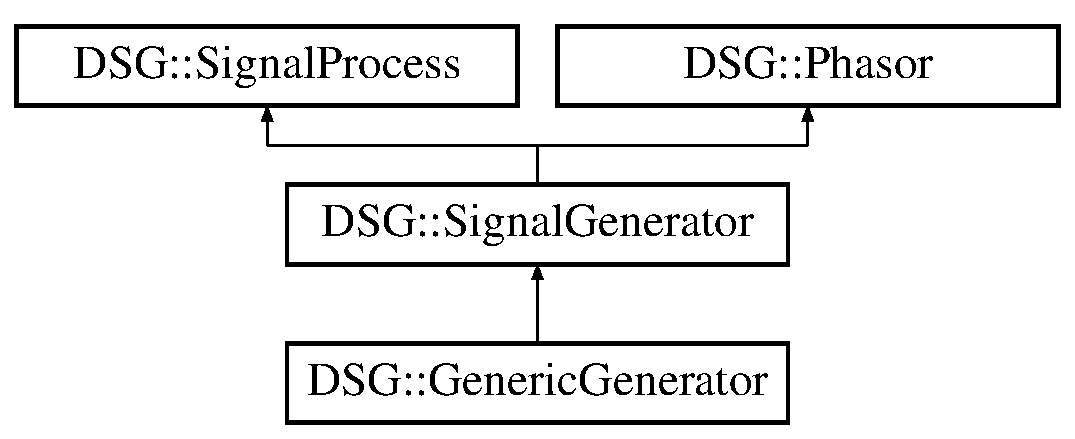
\includegraphics[height=3.000000cm]{class_d_s_g_1_1_generic_generator}
\end{center}
\end{figure}
\subsection*{Public Member Functions}
\begin{DoxyCompactItemize}
\item 
\hyperlink{class_d_s_g_1_1_generic_generator_a560df325ce43fa9a1baf4463ccaed2d3}{Generic\+Generator} ()
\item 
\hyperlink{class_d_s_g_1_1_generic_generator_a1dbab25aa71cb7bce7e4b02be5122244}{Generic\+Generator} (\hyperlink{namespace_d_s_g_a4315a061386fa1014fda09b15d3a6973}{D\+S\+G\+::\+D\+S\+G\+Frequency} const \&frequency, \hyperlink{namespace_d_s_g_a44431ce1eb0a7300efdd207bc879e52c}{D\+S\+G\+::\+D\+S\+G\+Phase} const \&offset, \hyperlink{namespace_d_s_g_ac39a94cd27ebcd9c1e7502d0c624894a}{D\+S\+G\+::\+D\+S\+G\+Sample}($\ast$signal\+Function)(\hyperlink{namespace_d_s_g_ac39a94cd27ebcd9c1e7502d0c624894a}{D\+S\+G\+::\+D\+S\+G\+Sample} const \&))
\item 
virtual \hyperlink{class_d_s_g_1_1_generic_generator_aeaca1efdba7186a8b3b1879b092e7bec}{$\sim$\+Generic\+Generator} ()
\item 
virtual bool \hyperlink{class_d_s_g_1_1_generic_generator_addcd9abbbf0e31f0af2ff18217a08302}{Perform} (\hyperlink{namespace_d_s_g_ac39a94cd27ebcd9c1e7502d0c624894a}{D\+S\+G\+::\+D\+S\+G\+Sample} \&signal)
\item 
virtual bool \hyperlink{class_d_s_g_1_1_generic_generator_a886544537d2f77243ec42dad9f124a8d}{Perform} (\hyperlink{class_d_s_g_1_1_ring_buffer}{D\+S\+G\+::\+Ring\+Buffer} \&signal)
\end{DoxyCompactItemize}
\subsection*{Protected Attributes}
\begin{DoxyCompactItemize}
\item 
\hyperlink{namespace_d_s_g_ac39a94cd27ebcd9c1e7502d0c624894a}{D\+S\+G\+::\+D\+S\+G\+Sample}($\ast$ \hyperlink{class_d_s_g_1_1_generic_generator_a0335953ca594a86f6059d4387e94b73d}{\+\_\+callback} )(\hyperlink{namespace_d_s_g_ac39a94cd27ebcd9c1e7502d0c624894a}{D\+S\+G\+::\+D\+S\+G\+Sample} const \&)
\end{DoxyCompactItemize}
\subsection*{Additional Inherited Members}


\subsection{Detailed Description}
\hyperlink{class_d_s_g_1_1_generic_generator}{D\+S\+G\+::\+Generic\+Generator} -\/ Generator designed to use a stateless generator function such as \hyperlink{namespace_d_s_g_aad63d316081c7d13a551acf346ee2749}{D\+S\+G\+::\+Sin()} 

Definition at line \hyperlink{_generic_generator_8h_source_l00029}{29} of file \hyperlink{_generic_generator_8h_source}{Generic\+Generator.\+h}.



\subsection{Constructor \& Destructor Documentation}
\hypertarget{class_d_s_g_1_1_generic_generator_a560df325ce43fa9a1baf4463ccaed2d3}{\index{D\+S\+G\+::\+Generic\+Generator@{D\+S\+G\+::\+Generic\+Generator}!Generic\+Generator@{Generic\+Generator}}
\index{Generic\+Generator@{Generic\+Generator}!D\+S\+G\+::\+Generic\+Generator@{D\+S\+G\+::\+Generic\+Generator}}
\subsubsection[{Generic\+Generator}]{\setlength{\rightskip}{0pt plus 5cm}D\+S\+G\+::\+Generic\+Generator\+::\+Generic\+Generator (
\begin{DoxyParamCaption}
{}
\end{DoxyParamCaption}
)}}\label{class_d_s_g_1_1_generic_generator_a560df325ce43fa9a1baf4463ccaed2d3}


Definition at line \hyperlink{_generic_generator_8cpp_source_l00025}{25} of file \hyperlink{_generic_generator_8cpp_source}{Generic\+Generator.\+cpp}.


\begin{DoxyCode}
00025 :\hyperlink{class_d_s_g_1_1_signal_generator}{DSG::SignalGenerator}()\{\}
\end{DoxyCode}
\hypertarget{class_d_s_g_1_1_generic_generator_a1dbab25aa71cb7bce7e4b02be5122244}{\index{D\+S\+G\+::\+Generic\+Generator@{D\+S\+G\+::\+Generic\+Generator}!Generic\+Generator@{Generic\+Generator}}
\index{Generic\+Generator@{Generic\+Generator}!D\+S\+G\+::\+Generic\+Generator@{D\+S\+G\+::\+Generic\+Generator}}
\subsubsection[{Generic\+Generator}]{\setlength{\rightskip}{0pt plus 5cm}D\+S\+G\+::\+Generic\+Generator\+::\+Generic\+Generator (
\begin{DoxyParamCaption}
\item[{{\bf D\+S\+G\+::\+D\+S\+G\+Frequency} const \&}]{frequency, }
\item[{{\bf D\+S\+G\+::\+D\+S\+G\+Phase} const \&}]{offset, }
\item[{{\bf D\+S\+G\+::\+D\+S\+G\+Sample}($\ast$)({\bf D\+S\+G\+::\+D\+S\+G\+Sample} const \&)}]{signal\+Function}
\end{DoxyParamCaption}
)}}\label{class_d_s_g_1_1_generic_generator_a1dbab25aa71cb7bce7e4b02be5122244}


Definition at line \hyperlink{_generic_generator_8cpp_source_l00026}{26} of file \hyperlink{_generic_generator_8cpp_source}{Generic\+Generator.\+cpp}.


\begin{DoxyCode}
00026 :\hyperlink{class_d_s_g_1_1_signal_generator}{DSG::SignalGenerator}(frequency,offset),\hyperlink{class_d_s_g_1_1_generic_generator_a0335953ca594a86f6059d4387e94b73d}{\_callback}(signalFunction)\{\}
\end{DoxyCode}
\hypertarget{class_d_s_g_1_1_generic_generator_aeaca1efdba7186a8b3b1879b092e7bec}{\index{D\+S\+G\+::\+Generic\+Generator@{D\+S\+G\+::\+Generic\+Generator}!````~Generic\+Generator@{$\sim$\+Generic\+Generator}}
\index{````~Generic\+Generator@{$\sim$\+Generic\+Generator}!D\+S\+G\+::\+Generic\+Generator@{D\+S\+G\+::\+Generic\+Generator}}
\subsubsection[{$\sim$\+Generic\+Generator}]{\setlength{\rightskip}{0pt plus 5cm}D\+S\+G\+::\+Generic\+Generator\+::$\sim$\+Generic\+Generator (
\begin{DoxyParamCaption}
{}
\end{DoxyParamCaption}
)\hspace{0.3cm}{\ttfamily [virtual]}}}\label{class_d_s_g_1_1_generic_generator_aeaca1efdba7186a8b3b1879b092e7bec}


Definition at line \hyperlink{_generic_generator_8cpp_source_l00027}{27} of file \hyperlink{_generic_generator_8cpp_source}{Generic\+Generator.\+cpp}.


\begin{DoxyCode}
00027 \{\}\end{DoxyCode}


\subsection{Member Function Documentation}
\hypertarget{class_d_s_g_1_1_generic_generator_addcd9abbbf0e31f0af2ff18217a08302}{\index{D\+S\+G\+::\+Generic\+Generator@{D\+S\+G\+::\+Generic\+Generator}!Perform@{Perform}}
\index{Perform@{Perform}!D\+S\+G\+::\+Generic\+Generator@{D\+S\+G\+::\+Generic\+Generator}}
\subsubsection[{Perform}]{\setlength{\rightskip}{0pt plus 5cm}bool D\+S\+G\+::\+Generic\+Generator\+::\+Perform (
\begin{DoxyParamCaption}
\item[{{\bf D\+S\+G\+::\+D\+S\+G\+Sample} \&}]{signal}
\end{DoxyParamCaption}
)\hspace{0.3cm}{\ttfamily [inline]}, {\ttfamily [virtual]}}}\label{class_d_s_g_1_1_generic_generator_addcd9abbbf0e31f0af2ff18217a08302}


Reimplemented from \hyperlink{class_d_s_g_1_1_signal_generator_a46fe75a81a242e191c5049d33ddf4155}{D\+S\+G\+::\+Signal\+Generator}.



Definition at line \hyperlink{_generic_generator_8h_source_l00039}{39} of file \hyperlink{_generic_generator_8h_source}{Generic\+Generator.\+h}.


\begin{DoxyCode}
00039                                                                 \{
00040         \textcolor{keywordflow}{if} (\hyperlink{class_d_s_g_1_1_generic_generator_a0335953ca594a86f6059d4387e94b73d}{\_callback}!=\textcolor{keyword}{nullptr}) \{
00041             signal = \hyperlink{class_d_s_g_1_1_generic_generator_a0335953ca594a86f6059d4387e94b73d}{\_callback}(\hyperlink{class_d_s_g_1_1_signal_generator_a1e23eb94e204b11db75fca030b951065}{\_phasor});
00042         \}\textcolor{keywordflow}{else} signal = 0;
00043         \hyperlink{class_d_s_g_1_1_signal_generator_a4c034c5b9ef3dc7548839288355643d5}{step}();
00044         \textcolor{keywordflow}{return} \textcolor{keyword}{true};
00045     \}
\end{DoxyCode}
\hypertarget{class_d_s_g_1_1_generic_generator_a886544537d2f77243ec42dad9f124a8d}{\index{D\+S\+G\+::\+Generic\+Generator@{D\+S\+G\+::\+Generic\+Generator}!Perform@{Perform}}
\index{Perform@{Perform}!D\+S\+G\+::\+Generic\+Generator@{D\+S\+G\+::\+Generic\+Generator}}
\subsubsection[{Perform}]{\setlength{\rightskip}{0pt plus 5cm}bool D\+S\+G\+::\+Generic\+Generator\+::\+Perform (
\begin{DoxyParamCaption}
\item[{{\bf D\+S\+G\+::\+Ring\+Buffer} \&}]{signal}
\end{DoxyParamCaption}
)\hspace{0.3cm}{\ttfamily [inline]}, {\ttfamily [virtual]}}}\label{class_d_s_g_1_1_generic_generator_a886544537d2f77243ec42dad9f124a8d}


Reimplemented from \hyperlink{class_d_s_g_1_1_signal_generator_ab050f80e84e6c8b3e354b56930d6a02b}{D\+S\+G\+::\+Signal\+Generator}.



Definition at line \hyperlink{_generic_generator_8h_source_l00046}{46} of file \hyperlink{_generic_generator_8h_source}{Generic\+Generator.\+h}.


\begin{DoxyCode}
00046                                                                  \{
00047         signal.\hyperlink{class_d_s_g_1_1_ring_buffer_ab23c8003d2857809a816068eeb209d60}{Flush}();
00048         \textcolor{keywordflow}{while} (!signal.\hyperlink{class_d_s_g_1_1_ring_buffer_a53ddb04ffcbb5470a8d2b0a3c65b70cb}{Full}()) \{
00049             \textcolor{keywordflow}{if} (\hyperlink{class_d_s_g_1_1_generic_generator_addcd9abbbf0e31f0af2ff18217a08302}{Perform}(\hyperlink{class_d_s_g_1_1_signal_generator_a28a9b47a1aa0783029f11a19ba0363f2}{\_storage})) \{
00050                 \textcolor{keywordflow}{if}(signal.\hyperlink{class_d_s_g_1_1_ring_buffer_aa5dd2caa0a270173251faee40a43d692}{Write}(\hyperlink{class_d_s_g_1_1_signal_generator_a28a9b47a1aa0783029f11a19ba0363f2}{\_storage}))\{
00051                 \}\textcolor{keywordflow}{else} \textcolor{keywordflow}{return} \textcolor{keyword}{false};
00052             \}\textcolor{keywordflow}{else} \textcolor{keywordflow}{return} \textcolor{keyword}{false};
00053         \}\textcolor{keywordflow}{return} \textcolor{keyword}{true};
00054     \}
\end{DoxyCode}


\subsection{Member Data Documentation}
\hypertarget{class_d_s_g_1_1_generic_generator_a0335953ca594a86f6059d4387e94b73d}{\index{D\+S\+G\+::\+Generic\+Generator@{D\+S\+G\+::\+Generic\+Generator}!\+\_\+callback@{\+\_\+callback}}
\index{\+\_\+callback@{\+\_\+callback}!D\+S\+G\+::\+Generic\+Generator@{D\+S\+G\+::\+Generic\+Generator}}
\subsubsection[{\+\_\+callback}]{\setlength{\rightskip}{0pt plus 5cm}{\bf D\+S\+G\+::\+D\+S\+G\+Sample}($\ast$ D\+S\+G\+::\+Generic\+Generator\+::\+\_\+callback)({\bf D\+S\+G\+::\+D\+S\+G\+Sample} const \&)\hspace{0.3cm}{\ttfamily [protected]}}}\label{class_d_s_g_1_1_generic_generator_a0335953ca594a86f6059d4387e94b73d}


Definition at line \hyperlink{_generic_generator_8h_source_l00037}{37} of file \hyperlink{_generic_generator_8h_source}{Generic\+Generator.\+h}.



The documentation for this class was generated from the following files\+:\begin{DoxyCompactItemize}
\item 
\hyperlink{_generic_generator_8h}{Generic\+Generator.\+h}\item 
\hyperlink{_generic_generator_8cpp}{Generic\+Generator.\+cpp}\end{DoxyCompactItemize}

\hypertarget{class_d_s_g_1_1_fourier_1_1_harmonic}{\section{D\+S\+G\+:\+:Fourier\+:\+:Harmonic Class Reference}
\label{class_d_s_g_1_1_fourier_1_1_harmonic}\index{D\+S\+G\+::\+Fourier\+::\+Harmonic@{D\+S\+G\+::\+Fourier\+::\+Harmonic}}
}


\hyperlink{class_d_s_g_1_1_fourier_1_1_harmonic}{D\+S\+G\+::\+Fourier\+::\+Harmonic} -\/ Represents a single harmonic in a \hyperlink{namespace_d_s_g_1_1_fourier}{Fourier} Series.  




{\ttfamily \#include $<$Fourier\+Series.\+h$>$}

\subsection*{Public Member Functions}
\begin{DoxyCompactItemize}
\item 
\hyperlink{class_d_s_g_1_1_fourier_1_1_harmonic_a5433617eaac39402d27ce24634140940}{Harmonic} ()
\item 
\hyperlink{class_d_s_g_1_1_fourier_1_1_harmonic_a1dbca63f18e7271f78ad466bacdad394}{Harmonic} (\hyperlink{namespace_d_s_g_ac39a94cd27ebcd9c1e7502d0c624894a}{D\+S\+G\+::\+D\+S\+G\+Sample} const \&ratio, \hyperlink{namespace_d_s_g_ac39a94cd27ebcd9c1e7502d0c624894a}{D\+S\+G\+::\+D\+S\+G\+Sample} const \&amplitude)
\item 
virtual \hyperlink{class_d_s_g_1_1_fourier_1_1_harmonic_aad4e5d3e4ef8cd53bf01b0624246b826}{$\sim$\+Harmonic} ()
\item 
\hyperlink{namespace_d_s_g_ac39a94cd27ebcd9c1e7502d0c624894a}{D\+S\+G\+::\+D\+S\+G\+Sample} const \& \hyperlink{class_d_s_g_1_1_fourier_1_1_harmonic_a26b2ccbb2f25f72040a555c51dc43672}{Ratio} () const 
\item 
\hyperlink{namespace_d_s_g_ac39a94cd27ebcd9c1e7502d0c624894a}{D\+S\+G\+::\+D\+S\+G\+Sample} const \& \hyperlink{class_d_s_g_1_1_fourier_1_1_harmonic_a013dc7cae9bd09dbc26193f5b501776f}{Ratio} (\hyperlink{namespace_d_s_g_ac39a94cd27ebcd9c1e7502d0c624894a}{D\+S\+G\+::\+D\+S\+G\+Sample} const \&value)
\item 
\hyperlink{namespace_d_s_g_ac39a94cd27ebcd9c1e7502d0c624894a}{D\+S\+G\+::\+D\+S\+G\+Sample} const \& \hyperlink{class_d_s_g_1_1_fourier_1_1_harmonic_a99175479a12ca8b6103eb58179777775}{Amplitude} () const 
\item 
\hyperlink{namespace_d_s_g_ac39a94cd27ebcd9c1e7502d0c624894a}{D\+S\+G\+::\+D\+S\+G\+Sample} const \& \hyperlink{class_d_s_g_1_1_fourier_1_1_harmonic_ae94f1868dfe70a1ea90cb86a5cc31a15}{Amplitude} (\hyperlink{namespace_d_s_g_ac39a94cd27ebcd9c1e7502d0c624894a}{D\+S\+G\+::\+D\+S\+G\+Sample} const \&value)
\end{DoxyCompactItemize}
\subsection*{Protected Attributes}
\begin{DoxyCompactItemize}
\item 
\hyperlink{namespace_d_s_g_ac39a94cd27ebcd9c1e7502d0c624894a}{D\+S\+G\+::\+D\+S\+G\+Sample} \hyperlink{class_d_s_g_1_1_fourier_1_1_harmonic_aa7138674df42fea66287ea31275bb14a}{\+\_\+ratio}
\item 
\hyperlink{namespace_d_s_g_ac39a94cd27ebcd9c1e7502d0c624894a}{D\+S\+G\+::\+D\+S\+G\+Sample} \hyperlink{class_d_s_g_1_1_fourier_1_1_harmonic_a76156f1ce5ccf45a9d4bfab38e932dfb}{\+\_\+amplitude}
\end{DoxyCompactItemize}


\subsection{Detailed Description}
\hyperlink{class_d_s_g_1_1_fourier_1_1_harmonic}{D\+S\+G\+::\+Fourier\+::\+Harmonic} -\/ Represents a single harmonic in a \hyperlink{namespace_d_s_g_1_1_fourier}{Fourier} Series. 

Definition at line \hyperlink{_fourier_series_8h_source_l00018}{18} of file \hyperlink{_fourier_series_8h_source}{Fourier\+Series.\+h}.



\subsection{Constructor \& Destructor Documentation}
\hypertarget{class_d_s_g_1_1_fourier_1_1_harmonic_a5433617eaac39402d27ce24634140940}{\index{D\+S\+G\+::\+Fourier\+::\+Harmonic@{D\+S\+G\+::\+Fourier\+::\+Harmonic}!Harmonic@{Harmonic}}
\index{Harmonic@{Harmonic}!D\+S\+G\+::\+Fourier\+::\+Harmonic@{D\+S\+G\+::\+Fourier\+::\+Harmonic}}
\subsubsection[{Harmonic}]{\setlength{\rightskip}{0pt plus 5cm}D\+S\+G\+::\+Fourier\+::\+Harmonic\+::\+Harmonic (
\begin{DoxyParamCaption}
{}
\end{DoxyParamCaption}
)}}\label{class_d_s_g_1_1_fourier_1_1_harmonic_a5433617eaac39402d27ce24634140940}


Definition at line \hyperlink{_fourier_series_8cpp_source_l00009}{9} of file \hyperlink{_fourier_series_8cpp_source}{Fourier\+Series.\+cpp}.


\begin{DoxyCode}
00009 :\hyperlink{class_d_s_g_1_1_fourier_1_1_harmonic_aa7138674df42fea66287ea31275bb14a}{\_ratio}(0),\hyperlink{class_d_s_g_1_1_fourier_1_1_harmonic_a76156f1ce5ccf45a9d4bfab38e932dfb}{\_amplitude}(0)\{\}
\end{DoxyCode}
\hypertarget{class_d_s_g_1_1_fourier_1_1_harmonic_a1dbca63f18e7271f78ad466bacdad394}{\index{D\+S\+G\+::\+Fourier\+::\+Harmonic@{D\+S\+G\+::\+Fourier\+::\+Harmonic}!Harmonic@{Harmonic}}
\index{Harmonic@{Harmonic}!D\+S\+G\+::\+Fourier\+::\+Harmonic@{D\+S\+G\+::\+Fourier\+::\+Harmonic}}
\subsubsection[{Harmonic}]{\setlength{\rightskip}{0pt plus 5cm}D\+S\+G\+::\+Fourier\+::\+Harmonic\+::\+Harmonic (
\begin{DoxyParamCaption}
\item[{{\bf D\+S\+G\+::\+D\+S\+G\+Sample} const \&}]{ratio, }
\item[{{\bf D\+S\+G\+::\+D\+S\+G\+Sample} const \&}]{amplitude}
\end{DoxyParamCaption}
)}}\label{class_d_s_g_1_1_fourier_1_1_harmonic_a1dbca63f18e7271f78ad466bacdad394}


Definition at line \hyperlink{_fourier_series_8cpp_source_l00010}{10} of file \hyperlink{_fourier_series_8cpp_source}{Fourier\+Series.\+cpp}.


\begin{DoxyCode}
00010 :\hyperlink{class_d_s_g_1_1_fourier_1_1_harmonic_aa7138674df42fea66287ea31275bb14a}{\_ratio}(ratio),\hyperlink{class_d_s_g_1_1_fourier_1_1_harmonic_a76156f1ce5ccf45a9d4bfab38e932dfb}{\_amplitude}(amplitude)\{\}
\end{DoxyCode}
\hypertarget{class_d_s_g_1_1_fourier_1_1_harmonic_aad4e5d3e4ef8cd53bf01b0624246b826}{\index{D\+S\+G\+::\+Fourier\+::\+Harmonic@{D\+S\+G\+::\+Fourier\+::\+Harmonic}!````~Harmonic@{$\sim$\+Harmonic}}
\index{````~Harmonic@{$\sim$\+Harmonic}!D\+S\+G\+::\+Fourier\+::\+Harmonic@{D\+S\+G\+::\+Fourier\+::\+Harmonic}}
\subsubsection[{$\sim$\+Harmonic}]{\setlength{\rightskip}{0pt plus 5cm}D\+S\+G\+::\+Fourier\+::\+Harmonic\+::$\sim$\+Harmonic (
\begin{DoxyParamCaption}
{}
\end{DoxyParamCaption}
)\hspace{0.3cm}{\ttfamily [virtual]}}}\label{class_d_s_g_1_1_fourier_1_1_harmonic_aad4e5d3e4ef8cd53bf01b0624246b826}


Definition at line \hyperlink{_fourier_series_8cpp_source_l00011}{11} of file \hyperlink{_fourier_series_8cpp_source}{Fourier\+Series.\+cpp}.


\begin{DoxyCode}
00011                              \{
00012     \hyperlink{class_d_s_g_1_1_fourier_1_1_harmonic_aa7138674df42fea66287ea31275bb14a}{\_ratio}=0;
00013     \hyperlink{class_d_s_g_1_1_fourier_1_1_harmonic_a76156f1ce5ccf45a9d4bfab38e932dfb}{\_amplitude}=0;
00014 \}
\end{DoxyCode}


\subsection{Member Function Documentation}
\hypertarget{class_d_s_g_1_1_fourier_1_1_harmonic_a99175479a12ca8b6103eb58179777775}{\index{D\+S\+G\+::\+Fourier\+::\+Harmonic@{D\+S\+G\+::\+Fourier\+::\+Harmonic}!Amplitude@{Amplitude}}
\index{Amplitude@{Amplitude}!D\+S\+G\+::\+Fourier\+::\+Harmonic@{D\+S\+G\+::\+Fourier\+::\+Harmonic}}
\subsubsection[{Amplitude}]{\setlength{\rightskip}{0pt plus 5cm}{\bf D\+S\+G\+::\+D\+S\+G\+Sample} const \& D\+S\+G\+::\+Fourier\+::\+Harmonic\+::\+Amplitude (
\begin{DoxyParamCaption}
{}
\end{DoxyParamCaption}
) const}}\label{class_d_s_g_1_1_fourier_1_1_harmonic_a99175479a12ca8b6103eb58179777775}


Definition at line \hyperlink{_fourier_series_8cpp_source_l00022}{22} of file \hyperlink{_fourier_series_8cpp_source}{Fourier\+Series.\+cpp}.


\begin{DoxyCode}
00022                                                       \{
00023     \textcolor{keywordflow}{return} \hyperlink{class_d_s_g_1_1_fourier_1_1_harmonic_a76156f1ce5ccf45a9d4bfab38e932dfb}{\_amplitude};
00024 \}
\end{DoxyCode}
\hypertarget{class_d_s_g_1_1_fourier_1_1_harmonic_ae94f1868dfe70a1ea90cb86a5cc31a15}{\index{D\+S\+G\+::\+Fourier\+::\+Harmonic@{D\+S\+G\+::\+Fourier\+::\+Harmonic}!Amplitude@{Amplitude}}
\index{Amplitude@{Amplitude}!D\+S\+G\+::\+Fourier\+::\+Harmonic@{D\+S\+G\+::\+Fourier\+::\+Harmonic}}
\subsubsection[{Amplitude}]{\setlength{\rightskip}{0pt plus 5cm}{\bf D\+S\+G\+::\+D\+S\+G\+Sample} const \& D\+S\+G\+::\+Fourier\+::\+Harmonic\+::\+Amplitude (
\begin{DoxyParamCaption}
\item[{{\bf D\+S\+G\+::\+D\+S\+G\+Sample} const \&}]{value}
\end{DoxyParamCaption}
)}}\label{class_d_s_g_1_1_fourier_1_1_harmonic_ae94f1868dfe70a1ea90cb86a5cc31a15}


Definition at line \hyperlink{_fourier_series_8cpp_source_l00025}{25} of file \hyperlink{_fourier_series_8cpp_source}{Fourier\+Series.\+cpp}.


\begin{DoxyCode}
00025                                                                           \{
00026     \hyperlink{class_d_s_g_1_1_fourier_1_1_harmonic_a76156f1ce5ccf45a9d4bfab38e932dfb}{\_amplitude}=value;
00027     \textcolor{keywordflow}{return} \hyperlink{class_d_s_g_1_1_fourier_1_1_harmonic_a76156f1ce5ccf45a9d4bfab38e932dfb}{\_amplitude};
00028 \}
\end{DoxyCode}
\hypertarget{class_d_s_g_1_1_fourier_1_1_harmonic_a26b2ccbb2f25f72040a555c51dc43672}{\index{D\+S\+G\+::\+Fourier\+::\+Harmonic@{D\+S\+G\+::\+Fourier\+::\+Harmonic}!Ratio@{Ratio}}
\index{Ratio@{Ratio}!D\+S\+G\+::\+Fourier\+::\+Harmonic@{D\+S\+G\+::\+Fourier\+::\+Harmonic}}
\subsubsection[{Ratio}]{\setlength{\rightskip}{0pt plus 5cm}{\bf D\+S\+G\+::\+D\+S\+G\+Sample} const \& D\+S\+G\+::\+Fourier\+::\+Harmonic\+::\+Ratio (
\begin{DoxyParamCaption}
{}
\end{DoxyParamCaption}
) const}}\label{class_d_s_g_1_1_fourier_1_1_harmonic_a26b2ccbb2f25f72040a555c51dc43672}


Definition at line \hyperlink{_fourier_series_8cpp_source_l00015}{15} of file \hyperlink{_fourier_series_8cpp_source}{Fourier\+Series.\+cpp}.


\begin{DoxyCode}
00015                                                   \{
00016     \textcolor{keywordflow}{return} \hyperlink{class_d_s_g_1_1_fourier_1_1_harmonic_aa7138674df42fea66287ea31275bb14a}{\_ratio};
00017 \}
\end{DoxyCode}
\hypertarget{class_d_s_g_1_1_fourier_1_1_harmonic_a013dc7cae9bd09dbc26193f5b501776f}{\index{D\+S\+G\+::\+Fourier\+::\+Harmonic@{D\+S\+G\+::\+Fourier\+::\+Harmonic}!Ratio@{Ratio}}
\index{Ratio@{Ratio}!D\+S\+G\+::\+Fourier\+::\+Harmonic@{D\+S\+G\+::\+Fourier\+::\+Harmonic}}
\subsubsection[{Ratio}]{\setlength{\rightskip}{0pt plus 5cm}{\bf D\+S\+G\+::\+D\+S\+G\+Sample} const \& D\+S\+G\+::\+Fourier\+::\+Harmonic\+::\+Ratio (
\begin{DoxyParamCaption}
\item[{{\bf D\+S\+G\+::\+D\+S\+G\+Sample} const \&}]{value}
\end{DoxyParamCaption}
)}}\label{class_d_s_g_1_1_fourier_1_1_harmonic_a013dc7cae9bd09dbc26193f5b501776f}


Definition at line \hyperlink{_fourier_series_8cpp_source_l00018}{18} of file \hyperlink{_fourier_series_8cpp_source}{Fourier\+Series.\+cpp}.


\begin{DoxyCode}
00018                                                                       \{
00019     \hyperlink{class_d_s_g_1_1_fourier_1_1_harmonic_aa7138674df42fea66287ea31275bb14a}{\_ratio} = value;
00020     \textcolor{keywordflow}{return} \hyperlink{class_d_s_g_1_1_fourier_1_1_harmonic_aa7138674df42fea66287ea31275bb14a}{\_ratio};
00021 \}
\end{DoxyCode}


\subsection{Member Data Documentation}
\hypertarget{class_d_s_g_1_1_fourier_1_1_harmonic_a76156f1ce5ccf45a9d4bfab38e932dfb}{\index{D\+S\+G\+::\+Fourier\+::\+Harmonic@{D\+S\+G\+::\+Fourier\+::\+Harmonic}!\+\_\+amplitude@{\+\_\+amplitude}}
\index{\+\_\+amplitude@{\+\_\+amplitude}!D\+S\+G\+::\+Fourier\+::\+Harmonic@{D\+S\+G\+::\+Fourier\+::\+Harmonic}}
\subsubsection[{\+\_\+amplitude}]{\setlength{\rightskip}{0pt plus 5cm}{\bf D\+S\+G\+::\+D\+S\+G\+Sample} D\+S\+G\+::\+Fourier\+::\+Harmonic\+::\+\_\+amplitude\hspace{0.3cm}{\ttfamily [protected]}}}\label{class_d_s_g_1_1_fourier_1_1_harmonic_a76156f1ce5ccf45a9d4bfab38e932dfb}


Definition at line \hyperlink{_fourier_series_8h_source_l00029}{29} of file \hyperlink{_fourier_series_8h_source}{Fourier\+Series.\+h}.

\hypertarget{class_d_s_g_1_1_fourier_1_1_harmonic_aa7138674df42fea66287ea31275bb14a}{\index{D\+S\+G\+::\+Fourier\+::\+Harmonic@{D\+S\+G\+::\+Fourier\+::\+Harmonic}!\+\_\+ratio@{\+\_\+ratio}}
\index{\+\_\+ratio@{\+\_\+ratio}!D\+S\+G\+::\+Fourier\+::\+Harmonic@{D\+S\+G\+::\+Fourier\+::\+Harmonic}}
\subsubsection[{\+\_\+ratio}]{\setlength{\rightskip}{0pt plus 5cm}{\bf D\+S\+G\+::\+D\+S\+G\+Sample} D\+S\+G\+::\+Fourier\+::\+Harmonic\+::\+\_\+ratio\hspace{0.3cm}{\ttfamily [protected]}}}\label{class_d_s_g_1_1_fourier_1_1_harmonic_aa7138674df42fea66287ea31275bb14a}


Definition at line \hyperlink{_fourier_series_8h_source_l00028}{28} of file \hyperlink{_fourier_series_8h_source}{Fourier\+Series.\+h}.



The documentation for this class was generated from the following files\+:\begin{DoxyCompactItemize}
\item 
/\+Users/alexanderzywicki/\+Documents/\+D\+S\+G/src/\hyperlink{_fourier_series_8h}{Fourier\+Series.\+h}\item 
/\+Users/alexanderzywicki/\+Documents/\+D\+S\+G/src/\hyperlink{_fourier_series_8cpp}{Fourier\+Series.\+cpp}\end{DoxyCompactItemize}

\hypertarget{class_d_s_g_1_1_filter_1_1_leaky_integrator}{\section{D\+S\+G\+:\+:Filter\+:\+:Leaky\+Integrator Class Reference}
\label{class_d_s_g_1_1_filter_1_1_leaky_integrator}\index{D\+S\+G\+::\+Filter\+::\+Leaky\+Integrator@{D\+S\+G\+::\+Filter\+::\+Leaky\+Integrator}}
}


\hyperlink{class_d_s_g_1_1_filter_1_1_leaky_integrator}{D\+S\+G\+::\+Filter\+::\+Leaky\+Integrator} -\/ Leaky integrator.  




{\ttfamily \#include $<$Leaky.\+h$>$}

Inheritance diagram for D\+S\+G\+:\+:Filter\+:\+:Leaky\+Integrator\+:\begin{figure}[H]
\begin{center}
\leavevmode
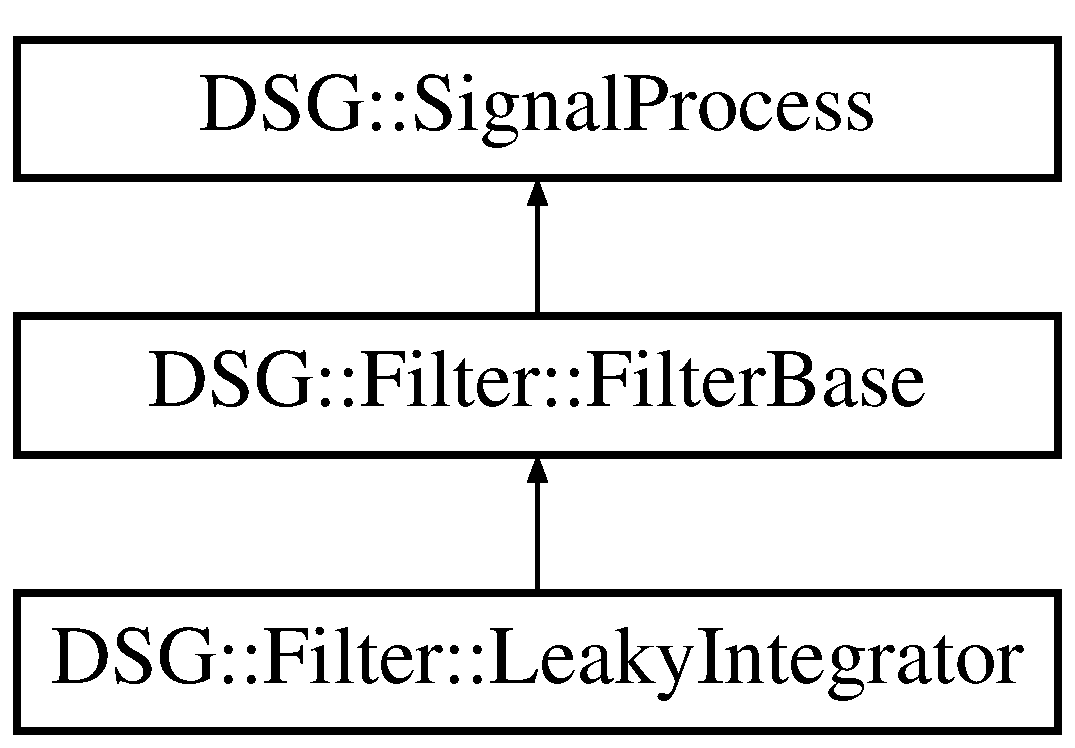
\includegraphics[height=3.000000cm]{class_d_s_g_1_1_filter_1_1_leaky_integrator}
\end{center}
\end{figure}
\subsection*{Public Member Functions}
\begin{DoxyCompactItemize}
\item 
\hyperlink{class_d_s_g_1_1_filter_1_1_leaky_integrator_af0d204e3c2f5f844dc4355810f6515c2}{Leaky\+Integrator} ()
\item 
\hyperlink{class_d_s_g_1_1_filter_1_1_leaky_integrator_ae50d8e7817b06cc64a45a6bc7aa657ff}{Leaky\+Integrator} (\hyperlink{namespace_d_s_g_a4315a061386fa1014fda09b15d3a6973}{D\+S\+G\+::\+D\+S\+G\+Frequency} const \&cutoff)
\item 
virtual \hyperlink{class_d_s_g_1_1_filter_1_1_leaky_integrator_a3a79cdbcf90a7924c05ec87b89fca83d}{$\sim$\+Leaky\+Integrator} ()
\item 
virtual bool \hyperlink{class_d_s_g_1_1_filter_1_1_leaky_integrator_a14ffd2f68de0cb9941d3295307ef13f0}{Perform} (\hyperlink{namespace_d_s_g_ac39a94cd27ebcd9c1e7502d0c624894a}{D\+S\+G\+::\+D\+S\+G\+Sample} \&signal)
\item 
virtual bool \hyperlink{class_d_s_g_1_1_filter_1_1_leaky_integrator_a7f094493387222422b9f283ec199dfd0}{Perform} (\hyperlink{class_d_s_g_1_1_ring_buffer}{D\+S\+G\+::\+Ring\+Buffer} \&signal)
\item 
virtual bool \hyperlink{class_d_s_g_1_1_filter_1_1_leaky_integrator_a5f326faae2d72a6550b2e0593b00eea6}{Cutoff} (\hyperlink{namespace_d_s_g_a4315a061386fa1014fda09b15d3a6973}{D\+S\+G\+::\+D\+S\+G\+Frequency} const \&cutoff)
\end{DoxyCompactItemize}
\subsection*{Protected Attributes}
\begin{DoxyCompactItemize}
\item 
double \hyperlink{class_d_s_g_1_1_filter_1_1_leaky_integrator_a052c709de4d6cddfdc0fb0441275ce98}{x1}
\item 
double \hyperlink{class_d_s_g_1_1_filter_1_1_leaky_integrator_a338246cc32a709070753696cf827624c}{y1}
\item 
double \hyperlink{class_d_s_g_1_1_filter_1_1_leaky_integrator_a9a321b7650923119fda60595a7659aef}{a}
\item 
double \hyperlink{class_d_s_g_1_1_filter_1_1_leaky_integrator_abb7e9fc15eef17836979b98b8b50880d}{b}
\item 
double \hyperlink{class_d_s_g_1_1_filter_1_1_leaky_integrator_a7b2591c401f8ee5196924de9c006ed74}{y}
\end{DoxyCompactItemize}


\subsection{Detailed Description}
\hyperlink{class_d_s_g_1_1_filter_1_1_leaky_integrator}{D\+S\+G\+::\+Filter\+::\+Leaky\+Integrator} -\/ Leaky integrator. 

Definition at line \hyperlink{_leaky_8h_source_l00019}{19} of file \hyperlink{_leaky_8h_source}{Leaky.\+h}.



\subsection{Constructor \& Destructor Documentation}
\hypertarget{class_d_s_g_1_1_filter_1_1_leaky_integrator_af0d204e3c2f5f844dc4355810f6515c2}{\index{D\+S\+G\+::\+Filter\+::\+Leaky\+Integrator@{D\+S\+G\+::\+Filter\+::\+Leaky\+Integrator}!Leaky\+Integrator@{Leaky\+Integrator}}
\index{Leaky\+Integrator@{Leaky\+Integrator}!D\+S\+G\+::\+Filter\+::\+Leaky\+Integrator@{D\+S\+G\+::\+Filter\+::\+Leaky\+Integrator}}
\subsubsection[{Leaky\+Integrator}]{\setlength{\rightskip}{0pt plus 5cm}D\+S\+G\+::\+Filter\+::\+Leaky\+Integrator\+::\+Leaky\+Integrator (
\begin{DoxyParamCaption}
{}
\end{DoxyParamCaption}
)}}\label{class_d_s_g_1_1_filter_1_1_leaky_integrator_af0d204e3c2f5f844dc4355810f6515c2}


Definition at line \hyperlink{_leaky_8cpp_source_l00009}{9} of file \hyperlink{_leaky_8cpp_source}{Leaky.\+cpp}.


\begin{DoxyCode}
00009                                          :\hyperlink{class_d_s_g_1_1_filter_1_1_filter_base}{DSG::Filter::FilterBase}()\{
00010     \hyperlink{class_d_s_g_1_1_filter_1_1_leaky_integrator_a052c709de4d6cddfdc0fb0441275ce98}{x1}=0;
00011     \hyperlink{class_d_s_g_1_1_filter_1_1_leaky_integrator_a338246cc32a709070753696cf827624c}{y1}=0;
00012     \hyperlink{class_d_s_g_1_1_filter_1_1_leaky_integrator_a9a321b7650923119fda60595a7659aef}{a}=0;
00013     \hyperlink{class_d_s_g_1_1_filter_1_1_leaky_integrator_abb7e9fc15eef17836979b98b8b50880d}{b}=0;
00014     \hyperlink{class_d_s_g_1_1_filter_1_1_leaky_integrator_a7b2591c401f8ee5196924de9c006ed74}{y}=0;
00015 \}
\end{DoxyCode}
\hypertarget{class_d_s_g_1_1_filter_1_1_leaky_integrator_ae50d8e7817b06cc64a45a6bc7aa657ff}{\index{D\+S\+G\+::\+Filter\+::\+Leaky\+Integrator@{D\+S\+G\+::\+Filter\+::\+Leaky\+Integrator}!Leaky\+Integrator@{Leaky\+Integrator}}
\index{Leaky\+Integrator@{Leaky\+Integrator}!D\+S\+G\+::\+Filter\+::\+Leaky\+Integrator@{D\+S\+G\+::\+Filter\+::\+Leaky\+Integrator}}
\subsubsection[{Leaky\+Integrator}]{\setlength{\rightskip}{0pt plus 5cm}D\+S\+G\+::\+Filter\+::\+Leaky\+Integrator\+::\+Leaky\+Integrator (
\begin{DoxyParamCaption}
\item[{{\bf D\+S\+G\+::\+D\+S\+G\+Frequency} const \&}]{cutoff}
\end{DoxyParamCaption}
)}}\label{class_d_s_g_1_1_filter_1_1_leaky_integrator_ae50d8e7817b06cc64a45a6bc7aa657ff}


Definition at line \hyperlink{_leaky_8cpp_source_l00016}{16} of file \hyperlink{_leaky_8cpp_source}{Leaky.\+cpp}.


\begin{DoxyCode}
00016                                                                       :
      \hyperlink{class_d_s_g_1_1_filter_1_1_filter_base}{DSG::Filter::FilterBase}()\{
00017     \hyperlink{class_d_s_g_1_1_filter_1_1_leaky_integrator_a052c709de4d6cddfdc0fb0441275ce98}{x1}=0;
00018     \hyperlink{class_d_s_g_1_1_filter_1_1_leaky_integrator_a338246cc32a709070753696cf827624c}{y1}=0;
00019     \hyperlink{class_d_s_g_1_1_filter_1_1_leaky_integrator_a9a321b7650923119fda60595a7659aef}{a}=0;
00020     \hyperlink{class_d_s_g_1_1_filter_1_1_leaky_integrator_abb7e9fc15eef17836979b98b8b50880d}{b}=0;
00021     \hyperlink{class_d_s_g_1_1_filter_1_1_leaky_integrator_a7b2591c401f8ee5196924de9c006ed74}{y}=0;
00022     \hyperlink{class_d_s_g_1_1_filter_1_1_leaky_integrator_a5f326faae2d72a6550b2e0593b00eea6}{Cutoff}(cutoff);
00023 \}
\end{DoxyCode}
\hypertarget{class_d_s_g_1_1_filter_1_1_leaky_integrator_a3a79cdbcf90a7924c05ec87b89fca83d}{\index{D\+S\+G\+::\+Filter\+::\+Leaky\+Integrator@{D\+S\+G\+::\+Filter\+::\+Leaky\+Integrator}!````~Leaky\+Integrator@{$\sim$\+Leaky\+Integrator}}
\index{````~Leaky\+Integrator@{$\sim$\+Leaky\+Integrator}!D\+S\+G\+::\+Filter\+::\+Leaky\+Integrator@{D\+S\+G\+::\+Filter\+::\+Leaky\+Integrator}}
\subsubsection[{$\sim$\+Leaky\+Integrator}]{\setlength{\rightskip}{0pt plus 5cm}D\+S\+G\+::\+Filter\+::\+Leaky\+Integrator\+::$\sim$\+Leaky\+Integrator (
\begin{DoxyParamCaption}
{}
\end{DoxyParamCaption}
)\hspace{0.3cm}{\ttfamily [virtual]}}}\label{class_d_s_g_1_1_filter_1_1_leaky_integrator_a3a79cdbcf90a7924c05ec87b89fca83d}


Definition at line \hyperlink{_leaky_8cpp_source_l00024}{24} of file \hyperlink{_leaky_8cpp_source}{Leaky.\+cpp}.


\begin{DoxyCode}
00024                                           \{
00025     \hyperlink{class_d_s_g_1_1_filter_1_1_leaky_integrator_a052c709de4d6cddfdc0fb0441275ce98}{x1}=0;
00026     \hyperlink{class_d_s_g_1_1_filter_1_1_leaky_integrator_a338246cc32a709070753696cf827624c}{y1}=0;
00027     \hyperlink{class_d_s_g_1_1_filter_1_1_leaky_integrator_a9a321b7650923119fda60595a7659aef}{a}=0;
00028     \hyperlink{class_d_s_g_1_1_filter_1_1_leaky_integrator_abb7e9fc15eef17836979b98b8b50880d}{b}=0;
00029     \hyperlink{class_d_s_g_1_1_filter_1_1_leaky_integrator_a7b2591c401f8ee5196924de9c006ed74}{y}=0;
00030 \}
\end{DoxyCode}


\subsection{Member Function Documentation}
\hypertarget{class_d_s_g_1_1_filter_1_1_leaky_integrator_a5f326faae2d72a6550b2e0593b00eea6}{\index{D\+S\+G\+::\+Filter\+::\+Leaky\+Integrator@{D\+S\+G\+::\+Filter\+::\+Leaky\+Integrator}!Cutoff@{Cutoff}}
\index{Cutoff@{Cutoff}!D\+S\+G\+::\+Filter\+::\+Leaky\+Integrator@{D\+S\+G\+::\+Filter\+::\+Leaky\+Integrator}}
\subsubsection[{Cutoff}]{\setlength{\rightskip}{0pt plus 5cm}bool D\+S\+G\+::\+Filter\+::\+Leaky\+Integrator\+::\+Cutoff (
\begin{DoxyParamCaption}
\item[{{\bf D\+S\+G\+::\+D\+S\+G\+Frequency} const \&}]{cutoff}
\end{DoxyParamCaption}
)\hspace{0.3cm}{\ttfamily [inline]}, {\ttfamily [virtual]}}}\label{class_d_s_g_1_1_filter_1_1_leaky_integrator_a5f326faae2d72a6550b2e0593b00eea6}


Reimplemented from \hyperlink{class_d_s_g_1_1_filter_1_1_filter_base_a1bf981bd2ca2151791d91b80dda827fe}{D\+S\+G\+::\+Filter\+::\+Filter\+Base}.



Definition at line \hyperlink{_leaky_8h_source_l00050}{50} of file \hyperlink{_leaky_8h_source}{Leaky.\+h}.


\begin{DoxyCode}
00050                                                                                  \{
00051             \textcolor{keywordtype}{double} Omega;
00052             \hyperlink{class_d_s_g_1_1_filter_1_1_leaky_integrator_a052c709de4d6cddfdc0fb0441275ce98}{x1} = \hyperlink{class_d_s_g_1_1_filter_1_1_leaky_integrator_a338246cc32a709070753696cf827624c}{y1} = 0.0;
00053             Omega = atan(\hyperlink{_p_i_8h_a598a3330b3c21701223ee0ca14316eca}{PI} * cutoff);
00054             \hyperlink{class_d_s_g_1_1_filter_1_1_leaky_integrator_a9a321b7650923119fda60595a7659aef}{a} = -(1.0 - Omega) / (1.0 + Omega);
00055             \hyperlink{class_d_s_g_1_1_filter_1_1_leaky_integrator_abb7e9fc15eef17836979b98b8b50880d}{b} = (1.0 - \hyperlink{class_d_s_g_1_1_filter_1_1_leaky_integrator_abb7e9fc15eef17836979b98b8b50880d}{b}) / 2.0;
00056             \textcolor{keywordflow}{return} \textcolor{keyword}{true};
00057         \}
\end{DoxyCode}
\hypertarget{class_d_s_g_1_1_filter_1_1_leaky_integrator_a14ffd2f68de0cb9941d3295307ef13f0}{\index{D\+S\+G\+::\+Filter\+::\+Leaky\+Integrator@{D\+S\+G\+::\+Filter\+::\+Leaky\+Integrator}!Perform@{Perform}}
\index{Perform@{Perform}!D\+S\+G\+::\+Filter\+::\+Leaky\+Integrator@{D\+S\+G\+::\+Filter\+::\+Leaky\+Integrator}}
\subsubsection[{Perform}]{\setlength{\rightskip}{0pt plus 5cm}bool D\+S\+G\+::\+Filter\+::\+Leaky\+Integrator\+::\+Perform (
\begin{DoxyParamCaption}
\item[{{\bf D\+S\+G\+::\+D\+S\+G\+Sample} \&}]{signal}
\end{DoxyParamCaption}
)\hspace{0.3cm}{\ttfamily [inline]}, {\ttfamily [virtual]}}}\label{class_d_s_g_1_1_filter_1_1_leaky_integrator_a14ffd2f68de0cb9941d3295307ef13f0}


Reimplemented from \hyperlink{class_d_s_g_1_1_filter_1_1_filter_base_ae7b6f59f5408ecab3ccd6c4e723c70b4}{D\+S\+G\+::\+Filter\+::\+Filter\+Base}.



Definition at line \hyperlink{_leaky_8h_source_l00031}{31} of file \hyperlink{_leaky_8h_source}{Leaky.\+h}.


\begin{DoxyCode}
00031                                                                          \{
00032             \hyperlink{class_d_s_g_1_1_filter_1_1_leaky_integrator_a7b2591c401f8ee5196924de9c006ed74}{y} = \hyperlink{class_d_s_g_1_1_filter_1_1_leaky_integrator_abb7e9fc15eef17836979b98b8b50880d}{b} * (signal + \hyperlink{class_d_s_g_1_1_filter_1_1_leaky_integrator_a052c709de4d6cddfdc0fb0441275ce98}{x1}) - \hyperlink{class_d_s_g_1_1_filter_1_1_leaky_integrator_a9a321b7650923119fda60595a7659aef}{a} * \hyperlink{class_d_s_g_1_1_filter_1_1_leaky_integrator_a338246cc32a709070753696cf827624c}{y1};
00033             \hyperlink{class_d_s_g_1_1_filter_1_1_leaky_integrator_a052c709de4d6cddfdc0fb0441275ce98}{x1}=signal;
00034             \hyperlink{class_d_s_g_1_1_filter_1_1_leaky_integrator_a338246cc32a709070753696cf827624c}{y1}=\hyperlink{class_d_s_g_1_1_filter_1_1_leaky_integrator_a7b2591c401f8ee5196924de9c006ed74}{y};
00035             signal=\hyperlink{class_d_s_g_1_1_filter_1_1_leaky_integrator_a7b2591c401f8ee5196924de9c006ed74}{y};
00036             \textcolor{keywordflow}{return} \textcolor{keyword}{true};
00037         \}
\end{DoxyCode}
\hypertarget{class_d_s_g_1_1_filter_1_1_leaky_integrator_a7f094493387222422b9f283ec199dfd0}{\index{D\+S\+G\+::\+Filter\+::\+Leaky\+Integrator@{D\+S\+G\+::\+Filter\+::\+Leaky\+Integrator}!Perform@{Perform}}
\index{Perform@{Perform}!D\+S\+G\+::\+Filter\+::\+Leaky\+Integrator@{D\+S\+G\+::\+Filter\+::\+Leaky\+Integrator}}
\subsubsection[{Perform}]{\setlength{\rightskip}{0pt plus 5cm}bool D\+S\+G\+::\+Filter\+::\+Leaky\+Integrator\+::\+Perform (
\begin{DoxyParamCaption}
\item[{{\bf D\+S\+G\+::\+Ring\+Buffer} \&}]{signal}
\end{DoxyParamCaption}
)\hspace{0.3cm}{\ttfamily [inline]}, {\ttfamily [virtual]}}}\label{class_d_s_g_1_1_filter_1_1_leaky_integrator_a7f094493387222422b9f283ec199dfd0}


Reimplemented from \hyperlink{class_d_s_g_1_1_filter_1_1_filter_base_aef58742a1362b7ef94574a16036b7109}{D\+S\+G\+::\+Filter\+::\+Filter\+Base}.



Definition at line \hyperlink{_leaky_8h_source_l00038}{38} of file \hyperlink{_leaky_8h_source}{Leaky.\+h}.


\begin{DoxyCode}
00038                                                                           \{
00039             \textcolor{keywordflow}{if} (!signal.\hyperlink{class_d_s_g_1_1_ring_buffer_ac1346f5842d08b988a5297abe4089b96}{Empty}()) \{
00040                 \hyperlink{class_d_s_g_1_1_filter_1_1_filter_base_a74068413169f9acb3fcf8276074e3b1d}{count} = signal.\hyperlink{class_d_s_g_1_1_ring_buffer_a9bd79b0a6dff618b205e396c101ee070}{Count}();
00041                 \textcolor{keywordflow}{while} (\hyperlink{class_d_s_g_1_1_filter_1_1_filter_base_a74068413169f9acb3fcf8276074e3b1d}{count}-- > 0) \{
00042                     \textcolor{keywordflow}{if}(signal.\hyperlink{class_d_s_g_1_1_ring_buffer_a6b2848a64f15c7b0c320779582fa0fbe}{Read}(\hyperlink{class_d_s_g_1_1_filter_1_1_filter_base_a9e21e909fa2989adb88eedcb194e0150}{\_temp}))\{
00043                         \textcolor{keywordflow}{if} (\hyperlink{class_d_s_g_1_1_filter_1_1_leaky_integrator_a14ffd2f68de0cb9941d3295307ef13f0}{Perform}(\hyperlink{class_d_s_g_1_1_filter_1_1_filter_base_a9e21e909fa2989adb88eedcb194e0150}{\_temp})) \{
00044                             signal.\hyperlink{class_d_s_g_1_1_ring_buffer_aa5dd2caa0a270173251faee40a43d692}{Write}(\hyperlink{class_d_s_g_1_1_filter_1_1_filter_base_a9e21e909fa2989adb88eedcb194e0150}{\_temp});
00045                         \}\textcolor{keywordflow}{else} \textcolor{keywordflow}{return} \textcolor{keyword}{false};
00046                     \}\textcolor{keywordflow}{else} \textcolor{keywordflow}{return} \textcolor{keyword}{false};
00047                 \}\textcolor{keywordflow}{return} \textcolor{keyword}{true};
00048             \}\textcolor{keywordflow}{else} \textcolor{keywordflow}{return} \textcolor{keyword}{false};
00049         \}
\end{DoxyCode}


\subsection{Member Data Documentation}
\hypertarget{class_d_s_g_1_1_filter_1_1_leaky_integrator_a9a321b7650923119fda60595a7659aef}{\index{D\+S\+G\+::\+Filter\+::\+Leaky\+Integrator@{D\+S\+G\+::\+Filter\+::\+Leaky\+Integrator}!a@{a}}
\index{a@{a}!D\+S\+G\+::\+Filter\+::\+Leaky\+Integrator@{D\+S\+G\+::\+Filter\+::\+Leaky\+Integrator}}
\subsubsection[{a}]{\setlength{\rightskip}{0pt plus 5cm}double D\+S\+G\+::\+Filter\+::\+Leaky\+Integrator\+::a\hspace{0.3cm}{\ttfamily [protected]}}}\label{class_d_s_g_1_1_filter_1_1_leaky_integrator_a9a321b7650923119fda60595a7659aef}


Definition at line \hyperlink{_leaky_8h_source_l00028}{28} of file \hyperlink{_leaky_8h_source}{Leaky.\+h}.

\hypertarget{class_d_s_g_1_1_filter_1_1_leaky_integrator_abb7e9fc15eef17836979b98b8b50880d}{\index{D\+S\+G\+::\+Filter\+::\+Leaky\+Integrator@{D\+S\+G\+::\+Filter\+::\+Leaky\+Integrator}!b@{b}}
\index{b@{b}!D\+S\+G\+::\+Filter\+::\+Leaky\+Integrator@{D\+S\+G\+::\+Filter\+::\+Leaky\+Integrator}}
\subsubsection[{b}]{\setlength{\rightskip}{0pt plus 5cm}double D\+S\+G\+::\+Filter\+::\+Leaky\+Integrator\+::b\hspace{0.3cm}{\ttfamily [protected]}}}\label{class_d_s_g_1_1_filter_1_1_leaky_integrator_abb7e9fc15eef17836979b98b8b50880d}


Definition at line \hyperlink{_leaky_8h_source_l00028}{28} of file \hyperlink{_leaky_8h_source}{Leaky.\+h}.

\hypertarget{class_d_s_g_1_1_filter_1_1_leaky_integrator_a052c709de4d6cddfdc0fb0441275ce98}{\index{D\+S\+G\+::\+Filter\+::\+Leaky\+Integrator@{D\+S\+G\+::\+Filter\+::\+Leaky\+Integrator}!x1@{x1}}
\index{x1@{x1}!D\+S\+G\+::\+Filter\+::\+Leaky\+Integrator@{D\+S\+G\+::\+Filter\+::\+Leaky\+Integrator}}
\subsubsection[{x1}]{\setlength{\rightskip}{0pt plus 5cm}double D\+S\+G\+::\+Filter\+::\+Leaky\+Integrator\+::x1\hspace{0.3cm}{\ttfamily [protected]}}}\label{class_d_s_g_1_1_filter_1_1_leaky_integrator_a052c709de4d6cddfdc0fb0441275ce98}


Definition at line \hyperlink{_leaky_8h_source_l00028}{28} of file \hyperlink{_leaky_8h_source}{Leaky.\+h}.

\hypertarget{class_d_s_g_1_1_filter_1_1_leaky_integrator_a7b2591c401f8ee5196924de9c006ed74}{\index{D\+S\+G\+::\+Filter\+::\+Leaky\+Integrator@{D\+S\+G\+::\+Filter\+::\+Leaky\+Integrator}!y@{y}}
\index{y@{y}!D\+S\+G\+::\+Filter\+::\+Leaky\+Integrator@{D\+S\+G\+::\+Filter\+::\+Leaky\+Integrator}}
\subsubsection[{y}]{\setlength{\rightskip}{0pt plus 5cm}double D\+S\+G\+::\+Filter\+::\+Leaky\+Integrator\+::y\hspace{0.3cm}{\ttfamily [protected]}}}\label{class_d_s_g_1_1_filter_1_1_leaky_integrator_a7b2591c401f8ee5196924de9c006ed74}


Definition at line \hyperlink{_leaky_8h_source_l00029}{29} of file \hyperlink{_leaky_8h_source}{Leaky.\+h}.

\hypertarget{class_d_s_g_1_1_filter_1_1_leaky_integrator_a338246cc32a709070753696cf827624c}{\index{D\+S\+G\+::\+Filter\+::\+Leaky\+Integrator@{D\+S\+G\+::\+Filter\+::\+Leaky\+Integrator}!y1@{y1}}
\index{y1@{y1}!D\+S\+G\+::\+Filter\+::\+Leaky\+Integrator@{D\+S\+G\+::\+Filter\+::\+Leaky\+Integrator}}
\subsubsection[{y1}]{\setlength{\rightskip}{0pt plus 5cm}double D\+S\+G\+::\+Filter\+::\+Leaky\+Integrator\+::y1\hspace{0.3cm}{\ttfamily [protected]}}}\label{class_d_s_g_1_1_filter_1_1_leaky_integrator_a338246cc32a709070753696cf827624c}


Definition at line \hyperlink{_leaky_8h_source_l00028}{28} of file \hyperlink{_leaky_8h_source}{Leaky.\+h}.



The documentation for this class was generated from the following files\+:\begin{DoxyCompactItemize}
\item 
/\+Users/alexanderzywicki/\+Documents/\+D\+S\+G/src/\hyperlink{_leaky_8h}{Leaky.\+h}\item 
/\+Users/alexanderzywicki/\+Documents/\+D\+S\+G/src/\hyperlink{_leaky_8cpp}{Leaky.\+cpp}\end{DoxyCompactItemize}

\hypertarget{class_d_s_g_1_1_l_u_t}{\section{D\+S\+G\+:\+:L\+U\+T$<$ element, size $>$ Class Template Reference}
\label{class_d_s_g_1_1_l_u_t}\index{D\+S\+G\+::\+L\+U\+T$<$ element, size $>$@{D\+S\+G\+::\+L\+U\+T$<$ element, size $>$}}
}
Inheritance diagram for D\+S\+G\+:\+:L\+U\+T$<$ element, size $>$\+:\begin{figure}[H]
\begin{center}
\leavevmode
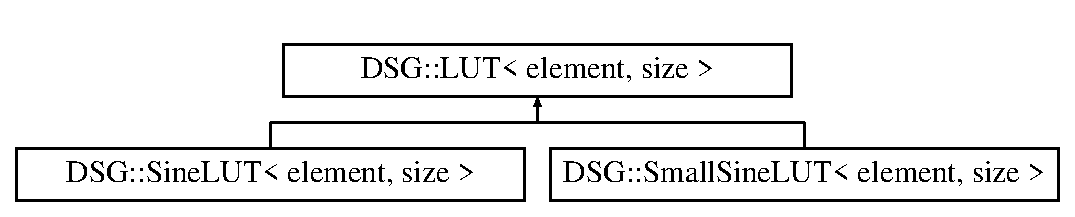
\includegraphics[height=2.000000cm]{class_d_s_g_1_1_l_u_t}
\end{center}
\end{figure}
\subsection*{Public Member Functions}
\begin{DoxyCompactItemize}
\item 
\hypertarget{class_d_s_g_1_1_l_u_t_a5f3bc252bd650fae13046e7959b94f81}{element const \& {\bfseries operator\mbox{[}$\,$\mbox{]}} (unsigned long const \&index)}\label{class_d_s_g_1_1_l_u_t_a5f3bc252bd650fae13046e7959b94f81}

\item 
\hypertarget{class_d_s_g_1_1_l_u_t_a131c3cf974754270699fdcda74f2e694}{virtual element const \& {\bfseries operator()} (double const \&x)}\label{class_d_s_g_1_1_l_u_t_a131c3cf974754270699fdcda74f2e694}

\item 
\hypertarget{class_d_s_g_1_1_l_u_t_a2d1a2112f9e960c7b70882a19d670ff9}{unsigned long const \& {\bfseries Size} () const }\label{class_d_s_g_1_1_l_u_t_a2d1a2112f9e960c7b70882a19d670ff9}

\end{DoxyCompactItemize}
\subsection*{Protected Attributes}
\begin{DoxyCompactItemize}
\item 
\hypertarget{class_d_s_g_1_1_l_u_t_ac8b23bbb7ce259d4ceb1c6fa93a7f29f}{element {\bfseries \+\_\+table} \mbox{[}size\mbox{]}}\label{class_d_s_g_1_1_l_u_t_ac8b23bbb7ce259d4ceb1c6fa93a7f29f}

\item 
\hypertarget{class_d_s_g_1_1_l_u_t_a87c352b5eaea2188955213c0f4ae9799}{const unsigned long {\bfseries \+\_\+size}}\label{class_d_s_g_1_1_l_u_t_a87c352b5eaea2188955213c0f4ae9799}

\end{DoxyCompactItemize}


The documentation for this class was generated from the following file\+:\begin{DoxyCompactItemize}
\item 
/\+Users/alexanderzywicki/\+Documents/\+D\+S\+G/src/L\+U\+T.\+h\end{DoxyCompactItemize}

\hypertarget{class_d_s_g_1_1_noise_generator}{\section{D\+S\+G\+:\+:Noise\+Generator Class Reference}
\label{class_d_s_g_1_1_noise_generator}\index{D\+S\+G\+::\+Noise\+Generator@{D\+S\+G\+::\+Noise\+Generator}}
}


\hyperlink{class_d_s_g_1_1_noise_generator}{D\+S\+G\+::\+Noise\+Generator} -\/ Generator that uses noise functions such as \hyperlink{namespace_d_s_g_1_1_noise_a0d1c4b4522d2e56b1aa604e45ab92066}{D\+S\+G\+::\+White()} to generate signal.  




{\ttfamily \#include $<$Noise\+Generator.\+h$>$}

Inheritance diagram for D\+S\+G\+:\+:Noise\+Generator\+:\begin{figure}[H]
\begin{center}
\leavevmode
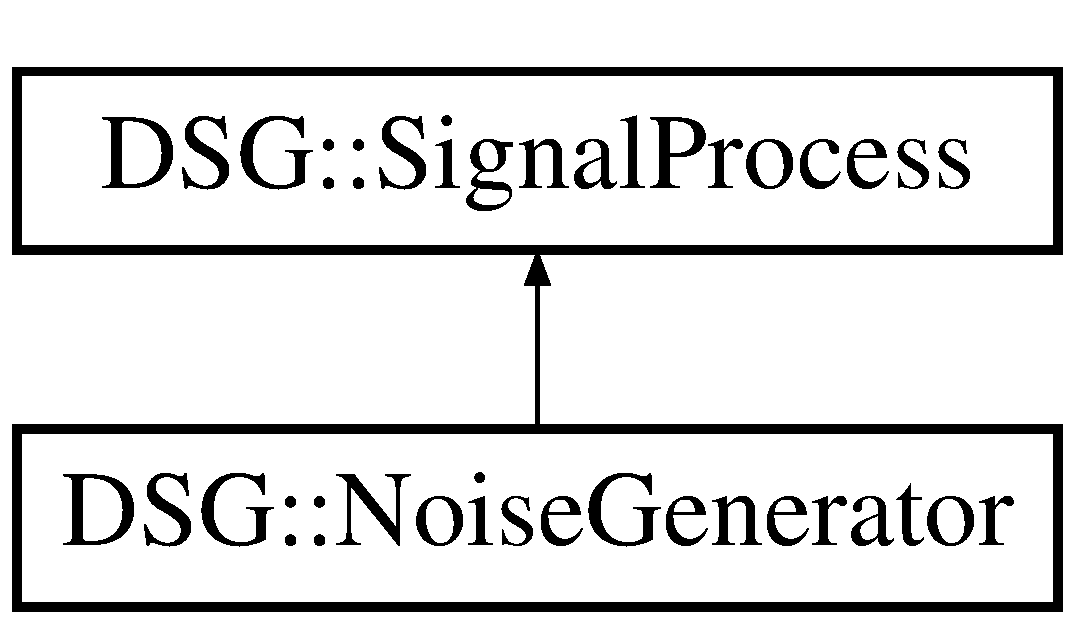
\includegraphics[height=2.000000cm]{class_d_s_g_1_1_noise_generator}
\end{center}
\end{figure}
\subsection*{Public Member Functions}
\begin{DoxyCompactItemize}
\item 
\hyperlink{class_d_s_g_1_1_noise_generator_ac78b8347da0c0593d495d9d054821c34}{Noise\+Generator} (\hyperlink{namespace_d_s_g_ac39a94cd27ebcd9c1e7502d0c624894a}{D\+S\+G\+Sample}($\ast$Stateless\+Function)(\hyperlink{namespace_d_s_g_ac39a94cd27ebcd9c1e7502d0c624894a}{D\+S\+G\+Sample}))
\item 
virtual \hyperlink{class_d_s_g_1_1_noise_generator_a964f0af791b5e09e63470bf42ddbce79}{$\sim$\+Noise\+Generator} ()
\item 
virtual bool \hyperlink{class_d_s_g_1_1_noise_generator_aa4f8426176cb0d461cbead361288f204}{Perform} (\hyperlink{namespace_d_s_g_ac39a94cd27ebcd9c1e7502d0c624894a}{D\+S\+G\+::\+D\+S\+G\+Sample} \&signal)
\item 
virtual bool \hyperlink{class_d_s_g_1_1_noise_generator_aee0a20c0a436c02f122a0f78664e99ec}{Perform} (\hyperlink{class_d_s_g_1_1_ring_buffer}{D\+S\+G\+::\+Ring\+Buffer} \&signal)
\end{DoxyCompactItemize}
\subsection*{Protected Attributes}
\begin{DoxyCompactItemize}
\item 
\hyperlink{namespace_d_s_g_ac39a94cd27ebcd9c1e7502d0c624894a}{D\+S\+G\+Sample}($\ast$ \hyperlink{class_d_s_g_1_1_noise_generator_a3fe30476196e0bfa22e314ce9bbd368b}{\+\_\+function} )(\hyperlink{namespace_d_s_g_ac39a94cd27ebcd9c1e7502d0c624894a}{D\+S\+G\+Sample})
\item 
\hyperlink{namespace_d_s_g_ac39a94cd27ebcd9c1e7502d0c624894a}{D\+S\+G\+::\+D\+S\+G\+Sample} \hyperlink{class_d_s_g_1_1_noise_generator_adb363b56bb2f621849fa457d54fc46a6}{\+\_\+storage}
\end{DoxyCompactItemize}


\subsection{Detailed Description}
\hyperlink{class_d_s_g_1_1_noise_generator}{D\+S\+G\+::\+Noise\+Generator} -\/ Generator that uses noise functions such as \hyperlink{namespace_d_s_g_1_1_noise_a0d1c4b4522d2e56b1aa604e45ab92066}{D\+S\+G\+::\+White()} to generate signal. 

Definition at line \hyperlink{_noise_generator_8h_source_l00013}{13} of file \hyperlink{_noise_generator_8h_source}{Noise\+Generator.\+h}.



\subsection{Constructor \& Destructor Documentation}
\hypertarget{class_d_s_g_1_1_noise_generator_ac78b8347da0c0593d495d9d054821c34}{\index{D\+S\+G\+::\+Noise\+Generator@{D\+S\+G\+::\+Noise\+Generator}!Noise\+Generator@{Noise\+Generator}}
\index{Noise\+Generator@{Noise\+Generator}!D\+S\+G\+::\+Noise\+Generator@{D\+S\+G\+::\+Noise\+Generator}}
\subsubsection[{Noise\+Generator}]{\setlength{\rightskip}{0pt plus 5cm}D\+S\+G\+::\+Noise\+Generator\+::\+Noise\+Generator (
\begin{DoxyParamCaption}
\item[{{\bf D\+S\+G\+Sample}($\ast$)({\bf D\+S\+G\+Sample})}]{Stateless\+Function}
\end{DoxyParamCaption}
)}}\label{class_d_s_g_1_1_noise_generator_ac78b8347da0c0593d495d9d054821c34}


Definition at line \hyperlink{_noise_generator_8cpp_source_l00009}{9} of file \hyperlink{_noise_generator_8cpp_source}{Noise\+Generator.\+cpp}.


\begin{DoxyCode}
00009                                                                           :
      \hyperlink{class_d_s_g_1_1_signal_process}{DSG::SignalProcess}()\{
00010     \hyperlink{class_d_s_g_1_1_noise_generator_a3fe30476196e0bfa22e314ce9bbd368b}{\_function} = StatelessFunction;
00011 \}
\end{DoxyCode}
\hypertarget{class_d_s_g_1_1_noise_generator_a964f0af791b5e09e63470bf42ddbce79}{\index{D\+S\+G\+::\+Noise\+Generator@{D\+S\+G\+::\+Noise\+Generator}!````~Noise\+Generator@{$\sim$\+Noise\+Generator}}
\index{````~Noise\+Generator@{$\sim$\+Noise\+Generator}!D\+S\+G\+::\+Noise\+Generator@{D\+S\+G\+::\+Noise\+Generator}}
\subsubsection[{$\sim$\+Noise\+Generator}]{\setlength{\rightskip}{0pt plus 5cm}D\+S\+G\+::\+Noise\+Generator\+::$\sim$\+Noise\+Generator (
\begin{DoxyParamCaption}
{}
\end{DoxyParamCaption}
)\hspace{0.3cm}{\ttfamily [virtual]}}}\label{class_d_s_g_1_1_noise_generator_a964f0af791b5e09e63470bf42ddbce79}


Definition at line \hyperlink{_noise_generator_8cpp_source_l00012}{12} of file \hyperlink{_noise_generator_8cpp_source}{Noise\+Generator.\+cpp}.


\begin{DoxyCode}
00012 \{\}
\end{DoxyCode}


\subsection{Member Function Documentation}
\hypertarget{class_d_s_g_1_1_noise_generator_aa4f8426176cb0d461cbead361288f204}{\index{D\+S\+G\+::\+Noise\+Generator@{D\+S\+G\+::\+Noise\+Generator}!Perform@{Perform}}
\index{Perform@{Perform}!D\+S\+G\+::\+Noise\+Generator@{D\+S\+G\+::\+Noise\+Generator}}
\subsubsection[{Perform}]{\setlength{\rightskip}{0pt plus 5cm}bool D\+S\+G\+::\+Noise\+Generator\+::\+Perform (
\begin{DoxyParamCaption}
\item[{{\bf D\+S\+G\+::\+D\+S\+G\+Sample} \&}]{signal}
\end{DoxyParamCaption}
)\hspace{0.3cm}{\ttfamily [inline]}, {\ttfamily [virtual]}}}\label{class_d_s_g_1_1_noise_generator_aa4f8426176cb0d461cbead361288f204}


Implements \hyperlink{class_d_s_g_1_1_signal_process_af73d246c460915db7a9be7e3ef36844d}{D\+S\+G\+::\+Signal\+Process}.



Definition at line \hyperlink{_noise_generator_8h_source_l00023}{23} of file \hyperlink{_noise_generator_8h_source}{Noise\+Generator.\+h}.


\begin{DoxyCode}
00023                                                               \{
00024         signal = \hyperlink{class_d_s_g_1_1_noise_generator_a3fe30476196e0bfa22e314ce9bbd368b}{\_function}(0);
00025         \textcolor{keywordflow}{return} \textcolor{keyword}{true};
00026     \}
\end{DoxyCode}
\hypertarget{class_d_s_g_1_1_noise_generator_aee0a20c0a436c02f122a0f78664e99ec}{\index{D\+S\+G\+::\+Noise\+Generator@{D\+S\+G\+::\+Noise\+Generator}!Perform@{Perform}}
\index{Perform@{Perform}!D\+S\+G\+::\+Noise\+Generator@{D\+S\+G\+::\+Noise\+Generator}}
\subsubsection[{Perform}]{\setlength{\rightskip}{0pt plus 5cm}bool D\+S\+G\+::\+Noise\+Generator\+::\+Perform (
\begin{DoxyParamCaption}
\item[{{\bf D\+S\+G\+::\+Ring\+Buffer} \&}]{signal}
\end{DoxyParamCaption}
)\hspace{0.3cm}{\ttfamily [inline]}, {\ttfamily [virtual]}}}\label{class_d_s_g_1_1_noise_generator_aee0a20c0a436c02f122a0f78664e99ec}


Implements \hyperlink{class_d_s_g_1_1_signal_process_a2c8ff3487d9c43f9eace1d9192d4a37e}{D\+S\+G\+::\+Signal\+Process}.



Definition at line \hyperlink{_noise_generator_8h_source_l00027}{27} of file \hyperlink{_noise_generator_8h_source}{Noise\+Generator.\+h}.


\begin{DoxyCode}
00027                                                                \{
00028         signal.\hyperlink{class_d_s_g_1_1_ring_buffer_ab23c8003d2857809a816068eeb209d60}{Flush}();
00029         \textcolor{keywordflow}{while} (!signal.\hyperlink{class_d_s_g_1_1_ring_buffer_a53ddb04ffcbb5470a8d2b0a3c65b70cb}{Full}()) \{
00030             \textcolor{keywordflow}{if} (\hyperlink{class_d_s_g_1_1_noise_generator_aa4f8426176cb0d461cbead361288f204}{Perform}(\hyperlink{class_d_s_g_1_1_noise_generator_adb363b56bb2f621849fa457d54fc46a6}{\_storage})) \{
00031                 \textcolor{keywordflow}{if}(signal.\hyperlink{class_d_s_g_1_1_ring_buffer_aa5dd2caa0a270173251faee40a43d692}{Write}(\hyperlink{class_d_s_g_1_1_noise_generator_adb363b56bb2f621849fa457d54fc46a6}{\_storage}))\{
00032                 \}\textcolor{keywordflow}{else} \textcolor{keywordflow}{return} \textcolor{keyword}{false};
00033             \}\textcolor{keywordflow}{else} \textcolor{keywordflow}{return} \textcolor{keyword}{false};
00034         \}\textcolor{keywordflow}{return} \textcolor{keyword}{true};
00035     \}
\end{DoxyCode}


\subsection{Member Data Documentation}
\hypertarget{class_d_s_g_1_1_noise_generator_a3fe30476196e0bfa22e314ce9bbd368b}{\index{D\+S\+G\+::\+Noise\+Generator@{D\+S\+G\+::\+Noise\+Generator}!\+\_\+function@{\+\_\+function}}
\index{\+\_\+function@{\+\_\+function}!D\+S\+G\+::\+Noise\+Generator@{D\+S\+G\+::\+Noise\+Generator}}
\subsubsection[{\+\_\+function}]{\setlength{\rightskip}{0pt plus 5cm}{\bf D\+S\+G\+Sample}($\ast$ D\+S\+G\+::\+Noise\+Generator\+::\+\_\+function)({\bf D\+S\+G\+Sample})\hspace{0.3cm}{\ttfamily [protected]}}}\label{class_d_s_g_1_1_noise_generator_a3fe30476196e0bfa22e314ce9bbd368b}


Definition at line \hyperlink{_noise_generator_8h_source_l00020}{20} of file \hyperlink{_noise_generator_8h_source}{Noise\+Generator.\+h}.

\hypertarget{class_d_s_g_1_1_noise_generator_adb363b56bb2f621849fa457d54fc46a6}{\index{D\+S\+G\+::\+Noise\+Generator@{D\+S\+G\+::\+Noise\+Generator}!\+\_\+storage@{\+\_\+storage}}
\index{\+\_\+storage@{\+\_\+storage}!D\+S\+G\+::\+Noise\+Generator@{D\+S\+G\+::\+Noise\+Generator}}
\subsubsection[{\+\_\+storage}]{\setlength{\rightskip}{0pt plus 5cm}{\bf D\+S\+G\+::\+D\+S\+G\+Sample} D\+S\+G\+::\+Noise\+Generator\+::\+\_\+storage\hspace{0.3cm}{\ttfamily [protected]}}}\label{class_d_s_g_1_1_noise_generator_adb363b56bb2f621849fa457d54fc46a6}


Definition at line \hyperlink{_noise_generator_8h_source_l00021}{21} of file \hyperlink{_noise_generator_8h_source}{Noise\+Generator.\+h}.



The documentation for this class was generated from the following files\+:\begin{DoxyCompactItemize}
\item 
/\+Users/alexanderzywicki/\+Documents/\+D\+S\+G/src/\hyperlink{_noise_generator_8h}{Noise\+Generator.\+h}\item 
/\+Users/alexanderzywicki/\+Documents/\+D\+S\+G/src/\hyperlink{_noise_generator_8cpp}{Noise\+Generator.\+cpp}\end{DoxyCompactItemize}

\hypertarget{class_d_s_g_1_1_ring_buffer}{\section{D\+S\+G\+:\+:Ring\+Buffer Class Reference}
\label{class_d_s_g_1_1_ring_buffer}\index{D\+S\+G\+::\+Ring\+Buffer@{D\+S\+G\+::\+Ring\+Buffer}}
}


\hyperlink{class_d_s_g_1_1_ring_buffer}{D\+S\+G\+::\+Ring\+Buffer} -\/ Circular \hyperlink{class_d_s_g_1_1_buffer}{Buffer} of Audio.  




{\ttfamily \#include $<$Ring\+Buffer.\+h$>$}

Inheritance diagram for D\+S\+G\+:\+:Ring\+Buffer\+:\begin{figure}[H]
\begin{center}
\leavevmode
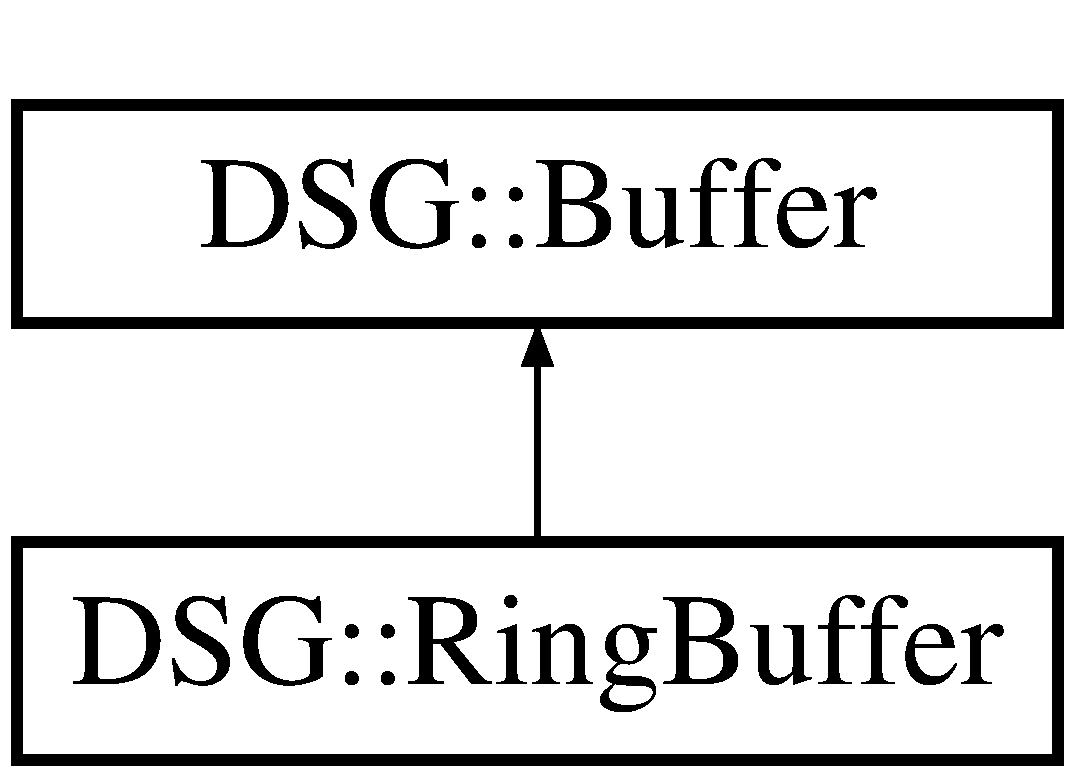
\includegraphics[height=2.000000cm]{class_d_s_g_1_1_ring_buffer}
\end{center}
\end{figure}
\subsection*{Public Member Functions}
\begin{DoxyCompactItemize}
\item 
\hyperlink{class_d_s_g_1_1_ring_buffer_a3136c9debb3c422adb1d5835e11b2b99}{Ring\+Buffer} ()
\item 
\hyperlink{class_d_s_g_1_1_ring_buffer_ae9859fd3ad18961de494d8b50fe4763e}{Ring\+Buffer} (const size\+\_\+t size)
\item 
\hyperlink{class_d_s_g_1_1_ring_buffer_ab09f32dacee49df3281c6701b7a4d737}{Ring\+Buffer} (\hyperlink{class_d_s_g_1_1_ring_buffer}{Ring\+Buffer} \&buffer)
\item 
\hyperlink{class_d_s_g_1_1_ring_buffer}{Ring\+Buffer} \& \hyperlink{class_d_s_g_1_1_ring_buffer_a892fbcc12b2dca5b04ead96a09299e73}{operator=} (\hyperlink{class_d_s_g_1_1_ring_buffer}{Ring\+Buffer} \&buffer)
\item 
virtual \hyperlink{class_d_s_g_1_1_ring_buffer_a771d30b04b6f0313c203530685fbeb3a}{$\sim$\+Ring\+Buffer} ()
\item 
bool \hyperlink{class_d_s_g_1_1_ring_buffer_aa5dd2caa0a270173251faee40a43d692}{Write} (const \hyperlink{namespace_d_s_g_ac39a94cd27ebcd9c1e7502d0c624894a}{D\+S\+G\+Sample} \&elem)
\item 
bool \hyperlink{class_d_s_g_1_1_ring_buffer_a6b2848a64f15c7b0c320779582fa0fbe}{Read} (\hyperlink{namespace_d_s_g_ac39a94cd27ebcd9c1e7502d0c624894a}{D\+S\+G\+::\+D\+S\+G\+Sample} \&elem)
\item 
size\+\_\+t const \& \hyperlink{class_d_s_g_1_1_ring_buffer_a9bd79b0a6dff618b205e396c101ee070}{Count} () const 
\item 
bool \hyperlink{class_d_s_g_1_1_ring_buffer_a53ddb04ffcbb5470a8d2b0a3c65b70cb}{Full} () const 
\item 
bool \hyperlink{class_d_s_g_1_1_ring_buffer_ac1346f5842d08b988a5297abe4089b96}{Empty} () const 
\item 
void \hyperlink{class_d_s_g_1_1_ring_buffer_ab23c8003d2857809a816068eeb209d60}{Flush} ()
\end{DoxyCompactItemize}
\subsection*{Protected Member Functions}
\begin{DoxyCompactItemize}
\item 
size\+\_\+t \hyperlink{class_d_s_g_1_1_ring_buffer_a6d7a76a4c9b38ccde46344662e08c9e5}{next} (size\+\_\+t current)
\item 
size\+\_\+t \hyperlink{class_d_s_g_1_1_ring_buffer_aaf481e139011e91b111cc048e726cafb}{make\+\_\+pow\+\_\+2} (size\+\_\+t number)
\end{DoxyCompactItemize}
\subsection*{Protected Attributes}
\begin{DoxyCompactItemize}
\item 
std\+::atomic$<$ size\+\_\+t $>$ \hyperlink{class_d_s_g_1_1_ring_buffer_a78bd7704fd059b745bc82421e1062123}{\+\_\+write}
\item 
std\+::atomic$<$ size\+\_\+t $>$ \hyperlink{class_d_s_g_1_1_ring_buffer_aa71bb75a5d24700be795a30e1a135a54}{\+\_\+read}
\item 
size\+\_\+t \hyperlink{class_d_s_g_1_1_ring_buffer_af6d0e1658a1f1aa298218b890e458f2f}{\+\_\+count}
\item 
size\+\_\+t \hyperlink{class_d_s_g_1_1_ring_buffer_a2fba2ff6ee3886101f0f58b0fd7f3641}{M\+A\+S\+K}
\item 
size\+\_\+t \hyperlink{class_d_s_g_1_1_ring_buffer_a703434b6afb87f1f9a05750278a822e3}{write}
\item 
size\+\_\+t \hyperlink{class_d_s_g_1_1_ring_buffer_a34bc659c286c8913e318c0e8c0777204}{read}
\end{DoxyCompactItemize}
\subsection*{Friends}
\begin{DoxyCompactItemize}
\item 
bool \hyperlink{class_d_s_g_1_1_ring_buffer_ab2e393fa39dc9b012eee8fe461e506cc}{operator$>$$>$} (\hyperlink{namespace_d_s_g_ac39a94cd27ebcd9c1e7502d0c624894a}{D\+S\+G\+::\+D\+S\+G\+Sample} const \&signal, \hyperlink{class_d_s_g_1_1_ring_buffer}{D\+S\+G\+::\+Ring\+Buffer} \&buffer)
\item 
bool \hyperlink{class_d_s_g_1_1_ring_buffer_a9eaa68fffdd0fcdccdccc0ee4a1ac711}{operator$<$$<$} (\hyperlink{namespace_d_s_g_ac39a94cd27ebcd9c1e7502d0c624894a}{D\+S\+G\+::\+D\+S\+G\+Sample} \&signal, \hyperlink{class_d_s_g_1_1_ring_buffer}{D\+S\+G\+::\+Ring\+Buffer} \&buffer)
\end{DoxyCompactItemize}


\subsection{Detailed Description}
\hyperlink{class_d_s_g_1_1_ring_buffer}{D\+S\+G\+::\+Ring\+Buffer} -\/ Circular \hyperlink{class_d_s_g_1_1_buffer}{Buffer} of Audio. 

Definition at line \hyperlink{_ring_buffer_8h_source_l00035}{35} of file \hyperlink{_ring_buffer_8h_source}{Ring\+Buffer.\+h}.



\subsection{Constructor \& Destructor Documentation}
\hypertarget{class_d_s_g_1_1_ring_buffer_a3136c9debb3c422adb1d5835e11b2b99}{\index{D\+S\+G\+::\+Ring\+Buffer@{D\+S\+G\+::\+Ring\+Buffer}!Ring\+Buffer@{Ring\+Buffer}}
\index{Ring\+Buffer@{Ring\+Buffer}!D\+S\+G\+::\+Ring\+Buffer@{D\+S\+G\+::\+Ring\+Buffer}}
\subsubsection[{Ring\+Buffer}]{\setlength{\rightskip}{0pt plus 5cm}D\+S\+G\+::\+Ring\+Buffer\+::\+Ring\+Buffer (
\begin{DoxyParamCaption}
{}
\end{DoxyParamCaption}
)}}\label{class_d_s_g_1_1_ring_buffer_a3136c9debb3c422adb1d5835e11b2b99}


Definition at line \hyperlink{_ring_buffer_8cpp_source_l00025}{25} of file \hyperlink{_ring_buffer_8cpp_source}{Ring\+Buffer.\+cpp}.


\begin{DoxyCode}
00025 :\hyperlink{class_d_s_g_1_1_buffer_aa764dd8c389dcff51de08cb81fafeb86}{Buffer}(0),\hyperlink{class_d_s_g_1_1_ring_buffer_aa71bb75a5d24700be795a30e1a135a54}{\_read}(0),\hyperlink{class_d_s_g_1_1_ring_buffer_a78bd7704fd059b745bc82421e1062123}{\_write}(0),\hyperlink{class_d_s_g_1_1_ring_buffer_af6d0e1658a1f1aa298218b890e458f2f}{\_count}(0),\hyperlink{class_d_s_g_1_1_ring_buffer_a2fba2ff6ee3886101f0f58b0fd7f3641}{MASK}(0)\{\}
\end{DoxyCode}
\hypertarget{class_d_s_g_1_1_ring_buffer_ae9859fd3ad18961de494d8b50fe4763e}{\index{D\+S\+G\+::\+Ring\+Buffer@{D\+S\+G\+::\+Ring\+Buffer}!Ring\+Buffer@{Ring\+Buffer}}
\index{Ring\+Buffer@{Ring\+Buffer}!D\+S\+G\+::\+Ring\+Buffer@{D\+S\+G\+::\+Ring\+Buffer}}
\subsubsection[{Ring\+Buffer}]{\setlength{\rightskip}{0pt plus 5cm}D\+S\+G\+::\+Ring\+Buffer\+::\+Ring\+Buffer (
\begin{DoxyParamCaption}
\item[{const size\+\_\+t}]{size}
\end{DoxyParamCaption}
)}}\label{class_d_s_g_1_1_ring_buffer_ae9859fd3ad18961de494d8b50fe4763e}


Definition at line \hyperlink{_ring_buffer_8cpp_source_l00026}{26} of file \hyperlink{_ring_buffer_8cpp_source}{Ring\+Buffer.\+cpp}.


\begin{DoxyCode}
00026                                            :\hyperlink{class_d_s_g_1_1_buffer_aa764dd8c389dcff51de08cb81fafeb86}{Buffer}(\hyperlink{class_d_s_g_1_1_ring_buffer_aaf481e139011e91b111cc048e726cafb}{make\_pow\_2}(size)),
      \hyperlink{class_d_s_g_1_1_ring_buffer_aa71bb75a5d24700be795a30e1a135a54}{\_read}(0),\hyperlink{class_d_s_g_1_1_ring_buffer_a78bd7704fd059b745bc82421e1062123}{\_write}(0),\hyperlink{class_d_s_g_1_1_ring_buffer_af6d0e1658a1f1aa298218b890e458f2f}{\_count}(0)\{
00027     \hyperlink{class_d_s_g_1_1_ring_buffer_a2fba2ff6ee3886101f0f58b0fd7f3641}{MASK} = this->\hyperlink{class_d_s_g_1_1_buffer_a4e2fef9ed617af2554b25c999def8f71}{\_size}-1;
00028 \}
\end{DoxyCode}
\hypertarget{class_d_s_g_1_1_ring_buffer_ab09f32dacee49df3281c6701b7a4d737}{\index{D\+S\+G\+::\+Ring\+Buffer@{D\+S\+G\+::\+Ring\+Buffer}!Ring\+Buffer@{Ring\+Buffer}}
\index{Ring\+Buffer@{Ring\+Buffer}!D\+S\+G\+::\+Ring\+Buffer@{D\+S\+G\+::\+Ring\+Buffer}}
\subsubsection[{Ring\+Buffer}]{\setlength{\rightskip}{0pt plus 5cm}D\+S\+G\+::\+Ring\+Buffer\+::\+Ring\+Buffer (
\begin{DoxyParamCaption}
\item[{{\bf Ring\+Buffer} \&}]{buffer}
\end{DoxyParamCaption}
)}}\label{class_d_s_g_1_1_ring_buffer_ab09f32dacee49df3281c6701b7a4d737}


Definition at line \hyperlink{_ring_buffer_8cpp_source_l00029}{29} of file \hyperlink{_ring_buffer_8cpp_source}{Ring\+Buffer.\+cpp}.


\begin{DoxyCode}
00029                                             :\hyperlink{class_d_s_g_1_1_buffer_aa764dd8c389dcff51de08cb81fafeb86}{Buffer}(buffer)\{
00030     \hyperlink{class_d_s_g_1_1_ring_buffer_a78bd7704fd059b745bc82421e1062123}{\_write}.store(buffer.\_write.load(std::memory\_order\_acquire));
00031     \hyperlink{class_d_s_g_1_1_ring_buffer_aa71bb75a5d24700be795a30e1a135a54}{\_read}.store(buffer.\_read.load(std::memory\_order\_acquire));
00032     \hyperlink{class_d_s_g_1_1_ring_buffer_af6d0e1658a1f1aa298218b890e458f2f}{\_count} = buffer.\_count;
00033     \hyperlink{class_d_s_g_1_1_ring_buffer_a2fba2ff6ee3886101f0f58b0fd7f3641}{MASK} = buffer.\_size-1;
00034 \}
\end{DoxyCode}
\hypertarget{class_d_s_g_1_1_ring_buffer_a771d30b04b6f0313c203530685fbeb3a}{\index{D\+S\+G\+::\+Ring\+Buffer@{D\+S\+G\+::\+Ring\+Buffer}!````~Ring\+Buffer@{$\sim$\+Ring\+Buffer}}
\index{````~Ring\+Buffer@{$\sim$\+Ring\+Buffer}!D\+S\+G\+::\+Ring\+Buffer@{D\+S\+G\+::\+Ring\+Buffer}}
\subsubsection[{$\sim$\+Ring\+Buffer}]{\setlength{\rightskip}{0pt plus 5cm}D\+S\+G\+::\+Ring\+Buffer\+::$\sim$\+Ring\+Buffer (
\begin{DoxyParamCaption}
{}
\end{DoxyParamCaption}
)\hspace{0.3cm}{\ttfamily [virtual]}}}\label{class_d_s_g_1_1_ring_buffer_a771d30b04b6f0313c203530685fbeb3a}


Definition at line \hyperlink{_ring_buffer_8cpp_source_l00043}{43} of file \hyperlink{_ring_buffer_8cpp_source}{Ring\+Buffer.\+cpp}.


\begin{DoxyCode}
00043 \{\hyperlink{class_d_s_g_1_1_ring_buffer_ab23c8003d2857809a816068eeb209d60}{Flush}();\}
\end{DoxyCode}


\subsection{Member Function Documentation}
\hypertarget{class_d_s_g_1_1_ring_buffer_a9bd79b0a6dff618b205e396c101ee070}{\index{D\+S\+G\+::\+Ring\+Buffer@{D\+S\+G\+::\+Ring\+Buffer}!Count@{Count}}
\index{Count@{Count}!D\+S\+G\+::\+Ring\+Buffer@{D\+S\+G\+::\+Ring\+Buffer}}
\subsubsection[{Count}]{\setlength{\rightskip}{0pt plus 5cm}size\+\_\+t const \& D\+S\+G\+::\+Ring\+Buffer\+::\+Count (
\begin{DoxyParamCaption}
{}
\end{DoxyParamCaption}
) const\hspace{0.3cm}{\ttfamily [inline]}}}\label{class_d_s_g_1_1_ring_buffer_a9bd79b0a6dff618b205e396c101ee070}


Definition at line \hyperlink{_ring_buffer_8h_source_l00106}{106} of file \hyperlink{_ring_buffer_8h_source}{Ring\+Buffer.\+h}.


\begin{DoxyCode}
00106                                                   \{
00107         \textcolor{keywordflow}{return} \hyperlink{class_d_s_g_1_1_ring_buffer_af6d0e1658a1f1aa298218b890e458f2f}{\_count};
00108     \}
\end{DoxyCode}
\hypertarget{class_d_s_g_1_1_ring_buffer_ac1346f5842d08b988a5297abe4089b96}{\index{D\+S\+G\+::\+Ring\+Buffer@{D\+S\+G\+::\+Ring\+Buffer}!Empty@{Empty}}
\index{Empty@{Empty}!D\+S\+G\+::\+Ring\+Buffer@{D\+S\+G\+::\+Ring\+Buffer}}
\subsubsection[{Empty}]{\setlength{\rightskip}{0pt plus 5cm}bool D\+S\+G\+::\+Ring\+Buffer\+::\+Empty (
\begin{DoxyParamCaption}
{}
\end{DoxyParamCaption}
) const\hspace{0.3cm}{\ttfamily [inline]}}}\label{class_d_s_g_1_1_ring_buffer_ac1346f5842d08b988a5297abe4089b96}


Definition at line \hyperlink{_ring_buffer_8h_source_l00080}{80} of file \hyperlink{_ring_buffer_8h_source}{Ring\+Buffer.\+h}.


\begin{DoxyCode}
00080                                          \{
00081         \textcolor{keywordflow}{return} \hyperlink{class_d_s_g_1_1_ring_buffer_af6d0e1658a1f1aa298218b890e458f2f}{\_count}==0;
00082     \}
\end{DoxyCode}
\hypertarget{class_d_s_g_1_1_ring_buffer_ab23c8003d2857809a816068eeb209d60}{\index{D\+S\+G\+::\+Ring\+Buffer@{D\+S\+G\+::\+Ring\+Buffer}!Flush@{Flush}}
\index{Flush@{Flush}!D\+S\+G\+::\+Ring\+Buffer@{D\+S\+G\+::\+Ring\+Buffer}}
\subsubsection[{Flush}]{\setlength{\rightskip}{0pt plus 5cm}void D\+S\+G\+::\+Ring\+Buffer\+::\+Flush (
\begin{DoxyParamCaption}
{}
\end{DoxyParamCaption}
)\hspace{0.3cm}{\ttfamily [inline]}}}\label{class_d_s_g_1_1_ring_buffer_ab23c8003d2857809a816068eeb209d60}


Definition at line \hyperlink{_ring_buffer_8h_source_l00083}{83} of file \hyperlink{_ring_buffer_8h_source}{Ring\+Buffer.\+h}.


\begin{DoxyCode}
00083                                     \{
00084         \hyperlink{class_d_s_g_1_1_ring_buffer_a78bd7704fd059b745bc82421e1062123}{\_write}.store(0,std::memory\_order\_relaxed);
00085         \hyperlink{class_d_s_g_1_1_ring_buffer_aa71bb75a5d24700be795a30e1a135a54}{\_read}.store(0,std::memory\_order\_relaxed);
00086         \hyperlink{class_d_s_g_1_1_ring_buffer_af6d0e1658a1f1aa298218b890e458f2f}{\_count}=0;
00087     \}
\end{DoxyCode}
\hypertarget{class_d_s_g_1_1_ring_buffer_a53ddb04ffcbb5470a8d2b0a3c65b70cb}{\index{D\+S\+G\+::\+Ring\+Buffer@{D\+S\+G\+::\+Ring\+Buffer}!Full@{Full}}
\index{Full@{Full}!D\+S\+G\+::\+Ring\+Buffer@{D\+S\+G\+::\+Ring\+Buffer}}
\subsubsection[{Full}]{\setlength{\rightskip}{0pt plus 5cm}bool D\+S\+G\+::\+Ring\+Buffer\+::\+Full (
\begin{DoxyParamCaption}
{}
\end{DoxyParamCaption}
) const\hspace{0.3cm}{\ttfamily [inline]}}}\label{class_d_s_g_1_1_ring_buffer_a53ddb04ffcbb5470a8d2b0a3c65b70cb}


Definition at line \hyperlink{_ring_buffer_8h_source_l00077}{77} of file \hyperlink{_ring_buffer_8h_source}{Ring\+Buffer.\+h}.


\begin{DoxyCode}
00077                                         \{
00078         \textcolor{keywordflow}{return} \hyperlink{class_d_s_g_1_1_ring_buffer_af6d0e1658a1f1aa298218b890e458f2f}{\_count}==this->\hyperlink{class_d_s_g_1_1_buffer_a4e2fef9ed617af2554b25c999def8f71}{\_size};
00079     \}
\end{DoxyCode}
\hypertarget{class_d_s_g_1_1_ring_buffer_aaf481e139011e91b111cc048e726cafb}{\index{D\+S\+G\+::\+Ring\+Buffer@{D\+S\+G\+::\+Ring\+Buffer}!make\+\_\+pow\+\_\+2@{make\+\_\+pow\+\_\+2}}
\index{make\+\_\+pow\+\_\+2@{make\+\_\+pow\+\_\+2}!D\+S\+G\+::\+Ring\+Buffer@{D\+S\+G\+::\+Ring\+Buffer}}
\subsubsection[{make\+\_\+pow\+\_\+2}]{\setlength{\rightskip}{0pt plus 5cm}size\+\_\+t D\+S\+G\+::\+Ring\+Buffer\+::make\+\_\+pow\+\_\+2 (
\begin{DoxyParamCaption}
\item[{size\+\_\+t}]{number}
\end{DoxyParamCaption}
)\hspace{0.3cm}{\ttfamily [inline]}, {\ttfamily [protected]}}}\label{class_d_s_g_1_1_ring_buffer_aaf481e139011e91b111cc048e726cafb}


Definition at line \hyperlink{_ring_buffer_8h_source_l00111}{111} of file \hyperlink{_ring_buffer_8h_source}{Ring\+Buffer.\+h}.


\begin{DoxyCode}
00111                                                         \{
00112         \textcolor{keywordflow}{return} pow(2, ceil(log(number)/log(2)));
00113     \}
\end{DoxyCode}
\hypertarget{class_d_s_g_1_1_ring_buffer_a6d7a76a4c9b38ccde46344662e08c9e5}{\index{D\+S\+G\+::\+Ring\+Buffer@{D\+S\+G\+::\+Ring\+Buffer}!next@{next}}
\index{next@{next}!D\+S\+G\+::\+Ring\+Buffer@{D\+S\+G\+::\+Ring\+Buffer}}
\subsubsection[{next}]{\setlength{\rightskip}{0pt plus 5cm}size\+\_\+t D\+S\+G\+::\+Ring\+Buffer\+::next (
\begin{DoxyParamCaption}
\item[{size\+\_\+t}]{current}
\end{DoxyParamCaption}
)\hspace{0.3cm}{\ttfamily [inline]}, {\ttfamily [protected]}}}\label{class_d_s_g_1_1_ring_buffer_a6d7a76a4c9b38ccde46344662e08c9e5}


Definition at line \hyperlink{_ring_buffer_8h_source_l00110}{110} of file \hyperlink{_ring_buffer_8h_source}{Ring\+Buffer.\+h}.


\begin{DoxyCode}
00110 \{\textcolor{keywordflow}{return} (current+1) & \hyperlink{class_d_s_g_1_1_ring_buffer_a2fba2ff6ee3886101f0f58b0fd7f3641}{MASK};\}
\end{DoxyCode}
\hypertarget{class_d_s_g_1_1_ring_buffer_a892fbcc12b2dca5b04ead96a09299e73}{\index{D\+S\+G\+::\+Ring\+Buffer@{D\+S\+G\+::\+Ring\+Buffer}!operator=@{operator=}}
\index{operator=@{operator=}!D\+S\+G\+::\+Ring\+Buffer@{D\+S\+G\+::\+Ring\+Buffer}}
\subsubsection[{operator=}]{\setlength{\rightskip}{0pt plus 5cm}{\bf D\+S\+G\+::\+Ring\+Buffer} \& D\+S\+G\+::\+Ring\+Buffer\+::operator= (
\begin{DoxyParamCaption}
\item[{{\bf Ring\+Buffer} \&}]{buffer}
\end{DoxyParamCaption}
)}}\label{class_d_s_g_1_1_ring_buffer_a892fbcc12b2dca5b04ead96a09299e73}


Definition at line \hyperlink{_ring_buffer_8cpp_source_l00035}{35} of file \hyperlink{_ring_buffer_8cpp_source}{Ring\+Buffer.\+cpp}.


\begin{DoxyCode}
00035                                                            \{
00036     \hyperlink{class_d_s_g_1_1_buffer_a977d572a7d402ff6bf991d7c5c0cc6a7}{Buffer::operator=}(buffer);
00037     \hyperlink{class_d_s_g_1_1_ring_buffer_a78bd7704fd059b745bc82421e1062123}{\_write}.store(buffer.\_write.load(std::memory\_order\_acquire));
00038     \hyperlink{class_d_s_g_1_1_ring_buffer_aa71bb75a5d24700be795a30e1a135a54}{\_read}.store(buffer.\_read.load(std::memory\_order\_acquire));
00039     \hyperlink{class_d_s_g_1_1_ring_buffer_af6d0e1658a1f1aa298218b890e458f2f}{\_count} = buffer.\_count;
00040     \hyperlink{class_d_s_g_1_1_ring_buffer_a2fba2ff6ee3886101f0f58b0fd7f3641}{MASK} = buffer.\_size-1;
00041     \textcolor{keywordflow}{return} *\textcolor{keyword}{this};
00042 \}
\end{DoxyCode}
\hypertarget{class_d_s_g_1_1_ring_buffer_a6b2848a64f15c7b0c320779582fa0fbe}{\index{D\+S\+G\+::\+Ring\+Buffer@{D\+S\+G\+::\+Ring\+Buffer}!Read@{Read}}
\index{Read@{Read}!D\+S\+G\+::\+Ring\+Buffer@{D\+S\+G\+::\+Ring\+Buffer}}
\subsubsection[{Read}]{\setlength{\rightskip}{0pt plus 5cm}bool D\+S\+G\+::\+Ring\+Buffer\+::\+Read (
\begin{DoxyParamCaption}
\item[{{\bf D\+S\+G\+::\+D\+S\+G\+Sample} \&}]{elem}
\end{DoxyParamCaption}
)\hspace{0.3cm}{\ttfamily [inline]}}}\label{class_d_s_g_1_1_ring_buffer_a6b2848a64f15c7b0c320779582fa0fbe}


Definition at line \hyperlink{_ring_buffer_8h_source_l00097}{97} of file \hyperlink{_ring_buffer_8h_source}{Ring\+Buffer.\+h}.


\begin{DoxyCode}
00097                                                   \{
00098         \textcolor{keywordflow}{if} (!\hyperlink{class_d_s_g_1_1_ring_buffer_ac1346f5842d08b988a5297abe4089b96}{Empty}()) \{
00099             \hyperlink{class_d_s_g_1_1_ring_buffer_a34bc659c286c8913e318c0e8c0777204}{read} = \hyperlink{class_d_s_g_1_1_ring_buffer_aa71bb75a5d24700be795a30e1a135a54}{\_read}.load(std::memory\_order\_acquire);
00100             \hyperlink{class_d_s_g_1_1_ring_buffer_aa71bb75a5d24700be795a30e1a135a54}{\_read}.store(\hyperlink{class_d_s_g_1_1_ring_buffer_a6d7a76a4c9b38ccde46344662e08c9e5}{next}(\hyperlink{class_d_s_g_1_1_ring_buffer_a34bc659c286c8913e318c0e8c0777204}{read}),std::memory\_order\_release);
00101             elem = this->\hyperlink{class_d_s_g_1_1_buffer_ae4a4db8fe44b62db18d6a7855b5773f9}{\_buffer}[\hyperlink{class_d_s_g_1_1_ring_buffer_a34bc659c286c8913e318c0e8c0777204}{read}];
00102             --\hyperlink{class_d_s_g_1_1_ring_buffer_af6d0e1658a1f1aa298218b890e458f2f}{\_count};
00103             \textcolor{keywordflow}{return} \textcolor{keyword}{true};
00104         \}\textcolor{keywordflow}{else} \textcolor{keywordflow}{return} \textcolor{keyword}{false};
00105     \}
\end{DoxyCode}
\hypertarget{class_d_s_g_1_1_ring_buffer_aa5dd2caa0a270173251faee40a43d692}{\index{D\+S\+G\+::\+Ring\+Buffer@{D\+S\+G\+::\+Ring\+Buffer}!Write@{Write}}
\index{Write@{Write}!D\+S\+G\+::\+Ring\+Buffer@{D\+S\+G\+::\+Ring\+Buffer}}
\subsubsection[{Write}]{\setlength{\rightskip}{0pt plus 5cm}bool D\+S\+G\+::\+Ring\+Buffer\+::\+Write (
\begin{DoxyParamCaption}
\item[{const {\bf D\+S\+G\+Sample} \&}]{elem}
\end{DoxyParamCaption}
)\hspace{0.3cm}{\ttfamily [inline]}}}\label{class_d_s_g_1_1_ring_buffer_aa5dd2caa0a270173251faee40a43d692}


Definition at line \hyperlink{_ring_buffer_8h_source_l00088}{88} of file \hyperlink{_ring_buffer_8h_source}{Ring\+Buffer.\+h}.


\begin{DoxyCode}
00088                                                          \{
00089         \textcolor{keywordflow}{if} (!\hyperlink{class_d_s_g_1_1_ring_buffer_a53ddb04ffcbb5470a8d2b0a3c65b70cb}{Full}()) \{
00090             \hyperlink{class_d_s_g_1_1_ring_buffer_a703434b6afb87f1f9a05750278a822e3}{write} = \hyperlink{class_d_s_g_1_1_ring_buffer_a78bd7704fd059b745bc82421e1062123}{\_write}.load(std::memory\_order\_acquire);
00091             \hyperlink{class_d_s_g_1_1_ring_buffer_a78bd7704fd059b745bc82421e1062123}{\_write}.store(\hyperlink{class_d_s_g_1_1_ring_buffer_a6d7a76a4c9b38ccde46344662e08c9e5}{next}(\hyperlink{class_d_s_g_1_1_ring_buffer_a703434b6afb87f1f9a05750278a822e3}{write}),std::memory\_order\_release);
00092             this->\hyperlink{class_d_s_g_1_1_buffer_ae4a4db8fe44b62db18d6a7855b5773f9}{\_buffer}[\hyperlink{class_d_s_g_1_1_ring_buffer_a703434b6afb87f1f9a05750278a822e3}{write}] = elem;
00093             ++\hyperlink{class_d_s_g_1_1_ring_buffer_af6d0e1658a1f1aa298218b890e458f2f}{\_count};
00094             \textcolor{keywordflow}{return} \textcolor{keyword}{true};
00095         \}\textcolor{keywordflow}{else} \textcolor{keywordflow}{return} \textcolor{keyword}{false};
00096     \}
\end{DoxyCode}


\subsection{Friends And Related Function Documentation}
\hypertarget{class_d_s_g_1_1_ring_buffer_a9eaa68fffdd0fcdccdccc0ee4a1ac711}{\index{D\+S\+G\+::\+Ring\+Buffer@{D\+S\+G\+::\+Ring\+Buffer}!operator$<$$<$@{operator$<$$<$}}
\index{operator$<$$<$@{operator$<$$<$}!D\+S\+G\+::\+Ring\+Buffer@{D\+S\+G\+::\+Ring\+Buffer}}
\subsubsection[{operator$<$$<$}]{\setlength{\rightskip}{0pt plus 5cm}bool operator$<$$<$ (
\begin{DoxyParamCaption}
\item[{{\bf D\+S\+G\+::\+D\+S\+G\+Sample} \&}]{signal, }
\item[{{\bf D\+S\+G\+::\+Ring\+Buffer} \&}]{buffer}
\end{DoxyParamCaption}
)\hspace{0.3cm}{\ttfamily [friend]}}}\label{class_d_s_g_1_1_ring_buffer_a9eaa68fffdd0fcdccdccc0ee4a1ac711}


Definition at line \hyperlink{_ring_buffer_8h_source_l00060}{60} of file \hyperlink{_ring_buffer_8h_source}{Ring\+Buffer.\+h}.


\begin{DoxyCode}
00060                                                                           \{
00061             \textcolor{keywordflow}{return} buffer.\hyperlink{class_d_s_g_1_1_ring_buffer_a6b2848a64f15c7b0c320779582fa0fbe}{Read}(signal);
00062         \}
\end{DoxyCode}
\hypertarget{class_d_s_g_1_1_ring_buffer_ab2e393fa39dc9b012eee8fe461e506cc}{\index{D\+S\+G\+::\+Ring\+Buffer@{D\+S\+G\+::\+Ring\+Buffer}!operator$>$$>$@{operator$>$$>$}}
\index{operator$>$$>$@{operator$>$$>$}!D\+S\+G\+::\+Ring\+Buffer@{D\+S\+G\+::\+Ring\+Buffer}}
\subsubsection[{operator$>$$>$}]{\setlength{\rightskip}{0pt plus 5cm}bool operator$>$$>$ (
\begin{DoxyParamCaption}
\item[{{\bf D\+S\+G\+::\+D\+S\+G\+Sample} const \&}]{signal, }
\item[{{\bf D\+S\+G\+::\+Ring\+Buffer} \&}]{buffer}
\end{DoxyParamCaption}
)\hspace{0.3cm}{\ttfamily [friend]}}}\label{class_d_s_g_1_1_ring_buffer_ab2e393fa39dc9b012eee8fe461e506cc}


Definition at line \hyperlink{_ring_buffer_8h_source_l00057}{57} of file \hyperlink{_ring_buffer_8h_source}{Ring\+Buffer.\+h}.


\begin{DoxyCode}
00057                                                                                 \{
00058             \textcolor{keywordflow}{return} buffer.\hyperlink{class_d_s_g_1_1_ring_buffer_aa5dd2caa0a270173251faee40a43d692}{Write}(signal);
00059         \}
\end{DoxyCode}


\subsection{Member Data Documentation}
\hypertarget{class_d_s_g_1_1_ring_buffer_af6d0e1658a1f1aa298218b890e458f2f}{\index{D\+S\+G\+::\+Ring\+Buffer@{D\+S\+G\+::\+Ring\+Buffer}!\+\_\+count@{\+\_\+count}}
\index{\+\_\+count@{\+\_\+count}!D\+S\+G\+::\+Ring\+Buffer@{D\+S\+G\+::\+Ring\+Buffer}}
\subsubsection[{\+\_\+count}]{\setlength{\rightskip}{0pt plus 5cm}size\+\_\+t D\+S\+G\+::\+Ring\+Buffer\+::\+\_\+count\hspace{0.3cm}{\ttfamily [protected]}}}\label{class_d_s_g_1_1_ring_buffer_af6d0e1658a1f1aa298218b890e458f2f}


Definition at line \hyperlink{_ring_buffer_8h_source_l00039}{39} of file \hyperlink{_ring_buffer_8h_source}{Ring\+Buffer.\+h}.

\hypertarget{class_d_s_g_1_1_ring_buffer_aa71bb75a5d24700be795a30e1a135a54}{\index{D\+S\+G\+::\+Ring\+Buffer@{D\+S\+G\+::\+Ring\+Buffer}!\+\_\+read@{\+\_\+read}}
\index{\+\_\+read@{\+\_\+read}!D\+S\+G\+::\+Ring\+Buffer@{D\+S\+G\+::\+Ring\+Buffer}}
\subsubsection[{\+\_\+read}]{\setlength{\rightskip}{0pt plus 5cm}std\+::atomic$<$size\+\_\+t$>$ D\+S\+G\+::\+Ring\+Buffer\+::\+\_\+read\hspace{0.3cm}{\ttfamily [protected]}}}\label{class_d_s_g_1_1_ring_buffer_aa71bb75a5d24700be795a30e1a135a54}


Definition at line \hyperlink{_ring_buffer_8h_source_l00038}{38} of file \hyperlink{_ring_buffer_8h_source}{Ring\+Buffer.\+h}.

\hypertarget{class_d_s_g_1_1_ring_buffer_a78bd7704fd059b745bc82421e1062123}{\index{D\+S\+G\+::\+Ring\+Buffer@{D\+S\+G\+::\+Ring\+Buffer}!\+\_\+write@{\+\_\+write}}
\index{\+\_\+write@{\+\_\+write}!D\+S\+G\+::\+Ring\+Buffer@{D\+S\+G\+::\+Ring\+Buffer}}
\subsubsection[{\+\_\+write}]{\setlength{\rightskip}{0pt plus 5cm}std\+::atomic$<$size\+\_\+t$>$ D\+S\+G\+::\+Ring\+Buffer\+::\+\_\+write\hspace{0.3cm}{\ttfamily [protected]}}}\label{class_d_s_g_1_1_ring_buffer_a78bd7704fd059b745bc82421e1062123}


Definition at line \hyperlink{_ring_buffer_8h_source_l00037}{37} of file \hyperlink{_ring_buffer_8h_source}{Ring\+Buffer.\+h}.

\hypertarget{class_d_s_g_1_1_ring_buffer_a2fba2ff6ee3886101f0f58b0fd7f3641}{\index{D\+S\+G\+::\+Ring\+Buffer@{D\+S\+G\+::\+Ring\+Buffer}!M\+A\+S\+K@{M\+A\+S\+K}}
\index{M\+A\+S\+K@{M\+A\+S\+K}!D\+S\+G\+::\+Ring\+Buffer@{D\+S\+G\+::\+Ring\+Buffer}}
\subsubsection[{M\+A\+S\+K}]{\setlength{\rightskip}{0pt plus 5cm}size\+\_\+t D\+S\+G\+::\+Ring\+Buffer\+::\+M\+A\+S\+K\hspace{0.3cm}{\ttfamily [protected]}}}\label{class_d_s_g_1_1_ring_buffer_a2fba2ff6ee3886101f0f58b0fd7f3641}


Definition at line \hyperlink{_ring_buffer_8h_source_l00040}{40} of file \hyperlink{_ring_buffer_8h_source}{Ring\+Buffer.\+h}.

\hypertarget{class_d_s_g_1_1_ring_buffer_a34bc659c286c8913e318c0e8c0777204}{\index{D\+S\+G\+::\+Ring\+Buffer@{D\+S\+G\+::\+Ring\+Buffer}!read@{read}}
\index{read@{read}!D\+S\+G\+::\+Ring\+Buffer@{D\+S\+G\+::\+Ring\+Buffer}}
\subsubsection[{read}]{\setlength{\rightskip}{0pt plus 5cm}size\+\_\+t D\+S\+G\+::\+Ring\+Buffer\+::read\hspace{0.3cm}{\ttfamily [protected]}}}\label{class_d_s_g_1_1_ring_buffer_a34bc659c286c8913e318c0e8c0777204}


Definition at line \hyperlink{_ring_buffer_8h_source_l00042}{42} of file \hyperlink{_ring_buffer_8h_source}{Ring\+Buffer.\+h}.

\hypertarget{class_d_s_g_1_1_ring_buffer_a703434b6afb87f1f9a05750278a822e3}{\index{D\+S\+G\+::\+Ring\+Buffer@{D\+S\+G\+::\+Ring\+Buffer}!write@{write}}
\index{write@{write}!D\+S\+G\+::\+Ring\+Buffer@{D\+S\+G\+::\+Ring\+Buffer}}
\subsubsection[{write}]{\setlength{\rightskip}{0pt plus 5cm}size\+\_\+t D\+S\+G\+::\+Ring\+Buffer\+::write\hspace{0.3cm}{\ttfamily [protected]}}}\label{class_d_s_g_1_1_ring_buffer_a703434b6afb87f1f9a05750278a822e3}


Definition at line \hyperlink{_ring_buffer_8h_source_l00041}{41} of file \hyperlink{_ring_buffer_8h_source}{Ring\+Buffer.\+h}.



The documentation for this class was generated from the following files\+:\begin{DoxyCompactItemize}
\item 
\hyperlink{_ring_buffer_8h}{Ring\+Buffer.\+h}\item 
\hyperlink{_ring_buffer_8cpp}{Ring\+Buffer.\+cpp}\end{DoxyCompactItemize}

\hypertarget{class_d_s_g_1_1_signal_generator}{\section{D\+S\+G\+:\+:Signal\+Generator Class Reference}
\label{class_d_s_g_1_1_signal_generator}\index{D\+S\+G\+::\+Signal\+Generator@{D\+S\+G\+::\+Signal\+Generator}}
}


\hyperlink{class_d_s_g_1_1_signal_generator}{D\+S\+G\+::\+Signal\+Generator} -\/ Extends D\+S\+G\+::\+Signal Process With Tools For Signal Generation.  




{\ttfamily \#include $<$Signal\+Generator.\+h$>$}

Inheritance diagram for D\+S\+G\+:\+:Signal\+Generator\+:\begin{figure}[H]
\begin{center}
\leavevmode
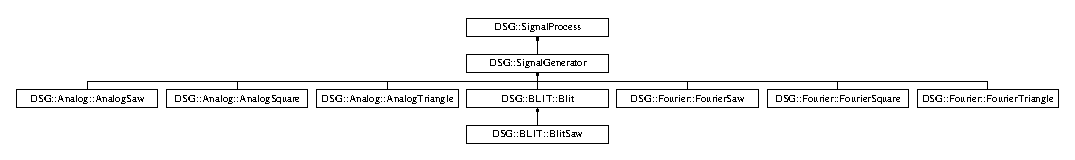
\includegraphics[height=12.000000cm]{class_d_s_g_1_1_signal_generator}
\end{center}
\end{figure}
\subsection*{Public Member Functions}
\begin{DoxyCompactItemize}
\item 
\hyperlink{class_d_s_g_1_1_signal_generator_a13ebda67fcdc880ef41aff501cc23fc3}{Signal\+Generator} ()
\item 
\hyperlink{class_d_s_g_1_1_signal_generator_a4036fceff5c05a3711b8516d850c414c}{Signal\+Generator} (\hyperlink{namespace_d_s_g_a4315a061386fa1014fda09b15d3a6973}{D\+S\+G\+::\+D\+S\+G\+Frequency} const \&frequency, \hyperlink{namespace_d_s_g_a44431ce1eb0a7300efdd207bc879e52c}{D\+S\+G\+::\+D\+S\+G\+Phase} const \&offset)
\item 
virtual \hyperlink{class_d_s_g_1_1_signal_generator_a7b52d391974bc36a19fdcf617ad976cb}{$\sim$\+Signal\+Generator} ()
\item 
virtual bool \hyperlink{class_d_s_g_1_1_signal_generator_a46fe75a81a242e191c5049d33ddf4155}{Perform} (\hyperlink{namespace_d_s_g_ac39a94cd27ebcd9c1e7502d0c624894a}{D\+S\+G\+::\+D\+S\+G\+Sample} \&signal)
\item 
virtual bool \hyperlink{class_d_s_g_1_1_signal_generator_ab050f80e84e6c8b3e354b56930d6a02b}{Perform} (\hyperlink{class_d_s_g_1_1_ring_buffer}{D\+S\+G\+::\+Ring\+Buffer} \&signal)
\item 
virtual \hyperlink{namespace_d_s_g_a4315a061386fa1014fda09b15d3a6973}{D\+S\+G\+::\+D\+S\+G\+Frequency} const \& \hyperlink{class_d_s_g_1_1_signal_generator_a4e6b3c43e76e53f8cd337ad699c464cb}{Frequency} ()
\item 
virtual \hyperlink{namespace_d_s_g_a4315a061386fa1014fda09b15d3a6973}{D\+S\+G\+::\+D\+S\+G\+Frequency} const \& \hyperlink{class_d_s_g_1_1_signal_generator_a30a79888f209d692df3d38f53fc58dfe}{Frequency} (\hyperlink{namespace_d_s_g_a4315a061386fa1014fda09b15d3a6973}{D\+S\+G\+::\+D\+S\+G\+Frequency} const \&value)
\item 
virtual \hyperlink{namespace_d_s_g_a44431ce1eb0a7300efdd207bc879e52c}{D\+S\+G\+::\+D\+S\+G\+Phase} const \& \hyperlink{class_d_s_g_1_1_signal_generator_a17cc4287b2838c6b6194fd43d02e7c00}{Phase} ()
\item 
virtual \hyperlink{namespace_d_s_g_a44431ce1eb0a7300efdd207bc879e52c}{D\+S\+G\+::\+D\+S\+G\+Phase} const \& \hyperlink{class_d_s_g_1_1_signal_generator_a315a3d3fca83eab7030af77dba63a564}{Phase} (\hyperlink{namespace_d_s_g_a44431ce1eb0a7300efdd207bc879e52c}{D\+S\+G\+::\+D\+S\+G\+Phase} const \&value)
\end{DoxyCompactItemize}
\subsection*{Protected Member Functions}
\begin{DoxyCompactItemize}
\item 
void \hyperlink{class_d_s_g_1_1_signal_generator_a4c034c5b9ef3dc7548839288355643d5}{step} ()
\item 
void \hyperlink{class_d_s_g_1_1_signal_generator_a7070f6be04dfd70170328e908b759cd3}{sync} ()
\end{DoxyCompactItemize}
\subsection*{Protected Attributes}
\begin{DoxyCompactItemize}
\item 
\hyperlink{namespace_d_s_g_a4315a061386fa1014fda09b15d3a6973}{D\+S\+G\+::\+D\+S\+G\+Frequency} \hyperlink{class_d_s_g_1_1_signal_generator_a335e7ef058848eca368be51d8544d143}{\+\_\+frequency}
\item 
\hyperlink{namespace_d_s_g_a44431ce1eb0a7300efdd207bc879e52c}{D\+S\+G\+::\+D\+S\+G\+Phase} \hyperlink{class_d_s_g_1_1_signal_generator_a01c046bb52bbb74afd789fdce7978f65}{\+\_\+dt}
\item 
\hyperlink{namespace_d_s_g_a44431ce1eb0a7300efdd207bc879e52c}{D\+S\+G\+::\+D\+S\+G\+Phase} \hyperlink{class_d_s_g_1_1_signal_generator_a12850f2c05838e2234602bd4fde87732}{\+\_\+offset}
\item 
\hyperlink{namespace_d_s_g_a44431ce1eb0a7300efdd207bc879e52c}{D\+S\+G\+::\+D\+S\+G\+Phase} \hyperlink{class_d_s_g_1_1_signal_generator_a1e23eb94e204b11db75fca030b951065}{\+\_\+phasor}
\item 
\hyperlink{namespace_d_s_g_ac39a94cd27ebcd9c1e7502d0c624894a}{D\+S\+G\+::\+D\+S\+G\+Sample} \hyperlink{class_d_s_g_1_1_signal_generator_a28a9b47a1aa0783029f11a19ba0363f2}{\+\_\+storage}
\end{DoxyCompactItemize}


\subsection{Detailed Description}
\hyperlink{class_d_s_g_1_1_signal_generator}{D\+S\+G\+::\+Signal\+Generator} -\/ Extends D\+S\+G\+::\+Signal Process With Tools For Signal Generation. 

Definition at line \hyperlink{_signal_generator_8h_source_l00033}{33} of file \hyperlink{_signal_generator_8h_source}{Signal\+Generator.\+h}.



\subsection{Constructor \& Destructor Documentation}
\hypertarget{class_d_s_g_1_1_signal_generator_a13ebda67fcdc880ef41aff501cc23fc3}{\index{D\+S\+G\+::\+Signal\+Generator@{D\+S\+G\+::\+Signal\+Generator}!Signal\+Generator@{Signal\+Generator}}
\index{Signal\+Generator@{Signal\+Generator}!D\+S\+G\+::\+Signal\+Generator@{D\+S\+G\+::\+Signal\+Generator}}
\subsubsection[{Signal\+Generator}]{\setlength{\rightskip}{0pt plus 5cm}D\+S\+G\+::\+Signal\+Generator\+::\+Signal\+Generator (
\begin{DoxyParamCaption}
{}
\end{DoxyParamCaption}
)}}\label{class_d_s_g_1_1_signal_generator_a13ebda67fcdc880ef41aff501cc23fc3}


Definition at line \hyperlink{_signal_generator_8cpp_source_l00025}{25} of file \hyperlink{_signal_generator_8cpp_source}{Signal\+Generator.\+cpp}.


\begin{DoxyCode}
00025 :\hyperlink{class_d_s_g_1_1_signal_process}{DSG::SignalProcess}(),\hyperlink{class_d_s_g_1_1_signal_generator_a1e23eb94e204b11db75fca030b951065}{\_phasor}(0),\hyperlink{class_d_s_g_1_1_signal_generator_a335e7ef058848eca368be51d8544d143}{\_frequency}(0),
      \hyperlink{class_d_s_g_1_1_signal_generator_a01c046bb52bbb74afd789fdce7978f65}{\_dt}(0),\hyperlink{class_d_s_g_1_1_signal_generator_a12850f2c05838e2234602bd4fde87732}{\_offset}(0)\{\}
\end{DoxyCode}
\hypertarget{class_d_s_g_1_1_signal_generator_a4036fceff5c05a3711b8516d850c414c}{\index{D\+S\+G\+::\+Signal\+Generator@{D\+S\+G\+::\+Signal\+Generator}!Signal\+Generator@{Signal\+Generator}}
\index{Signal\+Generator@{Signal\+Generator}!D\+S\+G\+::\+Signal\+Generator@{D\+S\+G\+::\+Signal\+Generator}}
\subsubsection[{Signal\+Generator}]{\setlength{\rightskip}{0pt plus 5cm}D\+S\+G\+::\+Signal\+Generator\+::\+Signal\+Generator (
\begin{DoxyParamCaption}
\item[{{\bf D\+S\+G\+::\+D\+S\+G\+Frequency} const \&}]{frequency, }
\item[{{\bf D\+S\+G\+::\+D\+S\+G\+Phase} const \&}]{offset}
\end{DoxyParamCaption}
)}}\label{class_d_s_g_1_1_signal_generator_a4036fceff5c05a3711b8516d850c414c}


Definition at line \hyperlink{_signal_generator_8cpp_source_l00026}{26} of file \hyperlink{_signal_generator_8cpp_source}{Signal\+Generator.\+cpp}.


\begin{DoxyCode}
00026                                                                                              :
      \hyperlink{class_d_s_g_1_1_signal_generator_a1e23eb94e204b11db75fca030b951065}{\_phasor}(0),\hyperlink{class_d_s_g_1_1_signal_generator_a335e7ef058848eca368be51d8544d143}{\_frequency}(frequency),\hyperlink{class_d_s_g_1_1_signal_generator_a01c046bb52bbb74afd789fdce7978f65}{\_dt}(0),\hyperlink{class_d_s_g_1_1_signal_generator_a12850f2c05838e2234602bd4fde87732}{\_offset}(offset)\{
00027     \hyperlink{class_d_s_g_1_1_signal_generator_a4e6b3c43e76e53f8cd337ad699c464cb}{Frequency}(frequency);
00028     \hyperlink{class_d_s_g_1_1_signal_generator_a17cc4287b2838c6b6194fd43d02e7c00}{Phase}(offset);
00029 \}
\end{DoxyCode}
\hypertarget{class_d_s_g_1_1_signal_generator_a7b52d391974bc36a19fdcf617ad976cb}{\index{D\+S\+G\+::\+Signal\+Generator@{D\+S\+G\+::\+Signal\+Generator}!````~Signal\+Generator@{$\sim$\+Signal\+Generator}}
\index{````~Signal\+Generator@{$\sim$\+Signal\+Generator}!D\+S\+G\+::\+Signal\+Generator@{D\+S\+G\+::\+Signal\+Generator}}
\subsubsection[{$\sim$\+Signal\+Generator}]{\setlength{\rightskip}{0pt plus 5cm}D\+S\+G\+::\+Signal\+Generator\+::$\sim$\+Signal\+Generator (
\begin{DoxyParamCaption}
{}
\end{DoxyParamCaption}
)\hspace{0.3cm}{\ttfamily [virtual]}}}\label{class_d_s_g_1_1_signal_generator_a7b52d391974bc36a19fdcf617ad976cb}


Definition at line \hyperlink{_signal_generator_8cpp_source_l00030}{30} of file \hyperlink{_signal_generator_8cpp_source}{Signal\+Generator.\+cpp}.


\begin{DoxyCode}
00030 \{\}\end{DoxyCode}


\subsection{Member Function Documentation}
\hypertarget{class_d_s_g_1_1_signal_generator_a4e6b3c43e76e53f8cd337ad699c464cb}{\index{D\+S\+G\+::\+Signal\+Generator@{D\+S\+G\+::\+Signal\+Generator}!Frequency@{Frequency}}
\index{Frequency@{Frequency}!D\+S\+G\+::\+Signal\+Generator@{D\+S\+G\+::\+Signal\+Generator}}
\subsubsection[{Frequency}]{\setlength{\rightskip}{0pt plus 5cm}{\bf D\+S\+G\+::\+D\+S\+G\+Frequency} const \& D\+S\+G\+::\+Signal\+Generator\+::\+Frequency (
\begin{DoxyParamCaption}
{}
\end{DoxyParamCaption}
)\hspace{0.3cm}{\ttfamily [inline]}, {\ttfamily [virtual]}}}\label{class_d_s_g_1_1_signal_generator_a4e6b3c43e76e53f8cd337ad699c464cb}


Definition at line \hyperlink{_signal_generator_8h_source_l00070}{70} of file \hyperlink{_signal_generator_8h_source}{Signal\+Generator.\+h}.


\begin{DoxyCode}
00070                                                            \{
00071     \textcolor{keywordflow}{return} \hyperlink{class_d_s_g_1_1_signal_generator_a335e7ef058848eca368be51d8544d143}{\_frequency};
00072 \}
\end{DoxyCode}
\hypertarget{class_d_s_g_1_1_signal_generator_a30a79888f209d692df3d38f53fc58dfe}{\index{D\+S\+G\+::\+Signal\+Generator@{D\+S\+G\+::\+Signal\+Generator}!Frequency@{Frequency}}
\index{Frequency@{Frequency}!D\+S\+G\+::\+Signal\+Generator@{D\+S\+G\+::\+Signal\+Generator}}
\subsubsection[{Frequency}]{\setlength{\rightskip}{0pt plus 5cm}{\bf D\+S\+G\+::\+D\+S\+G\+Frequency} const \& D\+S\+G\+::\+Signal\+Generator\+::\+Frequency (
\begin{DoxyParamCaption}
\item[{{\bf D\+S\+G\+::\+D\+S\+G\+Frequency} const \&}]{value}
\end{DoxyParamCaption}
)\hspace{0.3cm}{\ttfamily [inline]}, {\ttfamily [virtual]}}}\label{class_d_s_g_1_1_signal_generator_a30a79888f209d692df3d38f53fc58dfe}


Reimplemented in \hyperlink{class_d_s_g_1_1_b_l_i_t_1_1_blit_a933f8f9f324a4fde4f9e2b69473d88ed}{D\+S\+G\+::\+B\+L\+I\+T\+::\+Blit}, \hyperlink{class_d_s_g_1_1_b_l_i_t_1_1_blit_saw_a290d01796efca84b73eb61a3bc419ebb}{D\+S\+G\+::\+B\+L\+I\+T\+::\+Blit\+Saw}, \hyperlink{class_d_s_g_1_1_fourier_1_1_fourier_saw_afa3d86f404be3665f10c74fe9286ef10}{D\+S\+G\+::\+Fourier\+::\+Fourier\+Saw}, \hyperlink{class_d_s_g_1_1_fourier_1_1_fourier_square_a120cbb563a518c9412190eaa36cb269f}{D\+S\+G\+::\+Fourier\+::\+Fourier\+Square}, and \hyperlink{class_d_s_g_1_1_fourier_1_1_fourier_triangle_a278a51ed8af32ea371adc903b9b25039}{D\+S\+G\+::\+Fourier\+::\+Fourier\+Triangle}.



Definition at line \hyperlink{_signal_generator_8h_source_l00073}{73} of file \hyperlink{_signal_generator_8h_source}{Signal\+Generator.\+h}.


\begin{DoxyCode}
00073                                                                                        \{
00074     \hyperlink{class_d_s_g_1_1_signal_generator_a335e7ef058848eca368be51d8544d143}{\_frequency} = DSG::EnforceBounds<0, 20000,DSG::DSGSample>(value);
00075     \hyperlink{class_d_s_g_1_1_signal_generator_a01c046bb52bbb74afd789fdce7978f65}{\_dt} = \hyperlink{class_d_s_g_1_1_signal_generator_a335e7ef058848eca368be51d8544d143}{\_frequency}/\hyperlink{namespace_d_s_g_a72df05177db0412c3590070923f62819}{DSG::SampleRate}();
00076     \textcolor{keywordflow}{return} \hyperlink{class_d_s_g_1_1_signal_generator_a335e7ef058848eca368be51d8544d143}{\_frequency};
00077 \}
\end{DoxyCode}
\hypertarget{class_d_s_g_1_1_signal_generator_a46fe75a81a242e191c5049d33ddf4155}{\index{D\+S\+G\+::\+Signal\+Generator@{D\+S\+G\+::\+Signal\+Generator}!Perform@{Perform}}
\index{Perform@{Perform}!D\+S\+G\+::\+Signal\+Generator@{D\+S\+G\+::\+Signal\+Generator}}
\subsubsection[{Perform}]{\setlength{\rightskip}{0pt plus 5cm}bool D\+S\+G\+::\+Signal\+Generator\+::\+Perform (
\begin{DoxyParamCaption}
\item[{{\bf D\+S\+G\+::\+D\+S\+G\+Sample} \&}]{signal}
\end{DoxyParamCaption}
)\hspace{0.3cm}{\ttfamily [inline]}, {\ttfamily [virtual]}}}\label{class_d_s_g_1_1_signal_generator_a46fe75a81a242e191c5049d33ddf4155}


Implements \hyperlink{class_d_s_g_1_1_signal_process_af73d246c460915db7a9be7e3ef36844d}{D\+S\+G\+::\+Signal\+Process}.



Reimplemented in \hyperlink{class_d_s_g_1_1_fourier_1_1_fourier_series_generator_aa4768d44397b5fab5a30cb86068e161a}{D\+S\+G\+::\+Fourier\+::\+Fourier\+Series\+Generator}, \hyperlink{class_d_s_g_1_1_b_l_i_t_1_1_blit_adfd7c8891b4c4dbd0530a2780781b2bd}{D\+S\+G\+::\+B\+L\+I\+T\+::\+Blit}, \hyperlink{class_d_s_g_1_1_d_p_w_1_1_d_p_w_saw_a8d0bffad58e9bce19fe737302de749ed}{D\+S\+G\+::\+D\+P\+W\+::\+D\+P\+W\+Saw$<$ order $>$}, \hyperlink{class_d_s_g_1_1_e_p_t_r_1_1_e_p_t_r_saw_aa253efa41cca56f334ccb0fd32c2cd56}{D\+S\+G\+::\+E\+P\+T\+R\+::\+E\+P\+T\+R\+Saw}, \hyperlink{class_d_s_g_1_1_analog_1_1_analog_saw_a8d36e77c09ba84128e786c7bb14cddda}{D\+S\+G\+::\+Analog\+::\+Analog\+Saw}, \hyperlink{class_d_s_g_1_1_analog_1_1_analog_square_a784aa17d266704647789b972cf880e9f}{D\+S\+G\+::\+Analog\+::\+Analog\+Square}, \hyperlink{class_d_s_g_1_1_analog_1_1_analog_triangle_a9b2484f3eb4c4ad545cb88b8833be124}{D\+S\+G\+::\+Analog\+::\+Analog\+Triangle}, \hyperlink{class_d_s_g_1_1_b_l_i_t_1_1_blit_saw_ae24821c51b23b9fe9220a620e558af04}{D\+S\+G\+::\+B\+L\+I\+T\+::\+Blit\+Saw}, \hyperlink{class_d_s_g_1_1_fourier_1_1_fourier_saw_a33061612ff24180f12e9a2c29dfaa116}{D\+S\+G\+::\+Fourier\+::\+Fourier\+Saw}, \hyperlink{class_d_s_g_1_1_fourier_1_1_fourier_square_a05bd0cd3e76ca22e1cede5afb47fbbc4}{D\+S\+G\+::\+Fourier\+::\+Fourier\+Square}, \hyperlink{class_d_s_g_1_1_fourier_1_1_fourier_triangle_ab5b947c1fc1f34a461c863b18e3e877d}{D\+S\+G\+::\+Fourier\+::\+Fourier\+Triangle}, and \hyperlink{class_d_s_g_1_1_generic_generator_addcd9abbbf0e31f0af2ff18217a08302}{D\+S\+G\+::\+Generic\+Generator}.



Definition at line \hyperlink{_signal_generator_8h_source_l00062}{62} of file \hyperlink{_signal_generator_8h_source}{Signal\+Generator.\+h}.


\begin{DoxyCode}
00062                                                            \{
00063     signal=0;
00064     \textcolor{keywordflow}{return} \textcolor{keyword}{false};
00065 \}
\end{DoxyCode}
\hypertarget{class_d_s_g_1_1_signal_generator_ab050f80e84e6c8b3e354b56930d6a02b}{\index{D\+S\+G\+::\+Signal\+Generator@{D\+S\+G\+::\+Signal\+Generator}!Perform@{Perform}}
\index{Perform@{Perform}!D\+S\+G\+::\+Signal\+Generator@{D\+S\+G\+::\+Signal\+Generator}}
\subsubsection[{Perform}]{\setlength{\rightskip}{0pt plus 5cm}bool D\+S\+G\+::\+Signal\+Generator\+::\+Perform (
\begin{DoxyParamCaption}
\item[{{\bf D\+S\+G\+::\+Ring\+Buffer} \&}]{signal}
\end{DoxyParamCaption}
)\hspace{0.3cm}{\ttfamily [inline]}, {\ttfamily [virtual]}}}\label{class_d_s_g_1_1_signal_generator_ab050f80e84e6c8b3e354b56930d6a02b}


Implements \hyperlink{class_d_s_g_1_1_signal_process_a2c8ff3487d9c43f9eace1d9192d4a37e}{D\+S\+G\+::\+Signal\+Process}.



Reimplemented in \hyperlink{class_d_s_g_1_1_d_p_w_1_1_d_p_w_saw_a03548019c5ec057f5980a4bd99a0d3f0}{D\+S\+G\+::\+D\+P\+W\+::\+D\+P\+W\+Saw$<$ order $>$}, \hyperlink{class_d_s_g_1_1_fourier_1_1_fourier_series_generator_adce79a239104570f8a6565e708fb70a7}{D\+S\+G\+::\+Fourier\+::\+Fourier\+Series\+Generator}, \hyperlink{class_d_s_g_1_1_b_l_i_t_1_1_blit_aab7c67ff8f059c8367ba316cf8cd5436}{D\+S\+G\+::\+B\+L\+I\+T\+::\+Blit}, \hyperlink{class_d_s_g_1_1_e_p_t_r_1_1_e_p_t_r_saw_a9dbefaeeb74e30e722bb5d8ea767cdca}{D\+S\+G\+::\+E\+P\+T\+R\+::\+E\+P\+T\+R\+Saw}, \hyperlink{class_d_s_g_1_1_analog_1_1_analog_saw_a38f091059d924c9141fee3e27522e7e1}{D\+S\+G\+::\+Analog\+::\+Analog\+Saw}, \hyperlink{class_d_s_g_1_1_analog_1_1_analog_square_af4d41d5894ae02e920c61e06cf041c60}{D\+S\+G\+::\+Analog\+::\+Analog\+Square}, \hyperlink{class_d_s_g_1_1_analog_1_1_analog_triangle_a568c994e0f83f6a01d813357259a8f37}{D\+S\+G\+::\+Analog\+::\+Analog\+Triangle}, \hyperlink{class_d_s_g_1_1_b_l_i_t_1_1_blit_saw_ad2edba8ed83558e76afed6ec1d5cf4d6}{D\+S\+G\+::\+B\+L\+I\+T\+::\+Blit\+Saw}, \hyperlink{class_d_s_g_1_1_fourier_1_1_fourier_saw_ac890d9f0af523b63b96b07e6696a32b7}{D\+S\+G\+::\+Fourier\+::\+Fourier\+Saw}, \hyperlink{class_d_s_g_1_1_fourier_1_1_fourier_square_a46028a3615f26876f9c613f983141362}{D\+S\+G\+::\+Fourier\+::\+Fourier\+Square}, \hyperlink{class_d_s_g_1_1_fourier_1_1_fourier_triangle_a27b082e69cc7d70223dd3fbc552ba5bc}{D\+S\+G\+::\+Fourier\+::\+Fourier\+Triangle}, and \hyperlink{class_d_s_g_1_1_generic_generator_a886544537d2f77243ec42dad9f124a8d}{D\+S\+G\+::\+Generic\+Generator}.



Definition at line \hyperlink{_signal_generator_8h_source_l00066}{66} of file \hyperlink{_signal_generator_8h_source}{Signal\+Generator.\+h}.


\begin{DoxyCode}
00066                                                             \{
00067     signal.\hyperlink{class_d_s_g_1_1_ring_buffer_ab23c8003d2857809a816068eeb209d60}{Flush}();
00068     \textcolor{keywordflow}{return} \textcolor{keyword}{false};
00069 \}
\end{DoxyCode}
\hypertarget{class_d_s_g_1_1_signal_generator_a17cc4287b2838c6b6194fd43d02e7c00}{\index{D\+S\+G\+::\+Signal\+Generator@{D\+S\+G\+::\+Signal\+Generator}!Phase@{Phase}}
\index{Phase@{Phase}!D\+S\+G\+::\+Signal\+Generator@{D\+S\+G\+::\+Signal\+Generator}}
\subsubsection[{Phase}]{\setlength{\rightskip}{0pt plus 5cm}{\bf D\+S\+G\+::\+D\+S\+G\+Phase} const \& D\+S\+G\+::\+Signal\+Generator\+::\+Phase (
\begin{DoxyParamCaption}
{}
\end{DoxyParamCaption}
)\hspace{0.3cm}{\ttfamily [inline]}, {\ttfamily [virtual]}}}\label{class_d_s_g_1_1_signal_generator_a17cc4287b2838c6b6194fd43d02e7c00}


Definition at line \hyperlink{_signal_generator_8h_source_l00078}{78} of file \hyperlink{_signal_generator_8h_source}{Signal\+Generator.\+h}.


\begin{DoxyCode}
00078                                                    \{
00079     \textcolor{keywordflow}{return} \hyperlink{class_d_s_g_1_1_signal_generator_a12850f2c05838e2234602bd4fde87732}{\_offset};
00080 \}
\end{DoxyCode}
\hypertarget{class_d_s_g_1_1_signal_generator_a315a3d3fca83eab7030af77dba63a564}{\index{D\+S\+G\+::\+Signal\+Generator@{D\+S\+G\+::\+Signal\+Generator}!Phase@{Phase}}
\index{Phase@{Phase}!D\+S\+G\+::\+Signal\+Generator@{D\+S\+G\+::\+Signal\+Generator}}
\subsubsection[{Phase}]{\setlength{\rightskip}{0pt plus 5cm}{\bf D\+S\+G\+::\+D\+S\+G\+Phase} const \& D\+S\+G\+::\+Signal\+Generator\+::\+Phase (
\begin{DoxyParamCaption}
\item[{{\bf D\+S\+G\+::\+D\+S\+G\+Phase} const \&}]{value}
\end{DoxyParamCaption}
)\hspace{0.3cm}{\ttfamily [inline]}, {\ttfamily [virtual]}}}\label{class_d_s_g_1_1_signal_generator_a315a3d3fca83eab7030af77dba63a564}


Definition at line \hyperlink{_signal_generator_8h_source_l00081}{81} of file \hyperlink{_signal_generator_8h_source}{Signal\+Generator.\+h}.


\begin{DoxyCode}
00081                                                                            \{
00082     \hyperlink{class_d_s_g_1_1_signal_generator_a12850f2c05838e2234602bd4fde87732}{\_offset}-=value;
00083     \hyperlink{class_d_s_g_1_1_signal_generator_a1e23eb94e204b11db75fca030b951065}{\_phasor}-=\hyperlink{class_d_s_g_1_1_signal_generator_a12850f2c05838e2234602bd4fde87732}{\_offset};
00084     \hyperlink{class_d_s_g_1_1_signal_generator_a12850f2c05838e2234602bd4fde87732}{\_offset}=value;
00085     \textcolor{keywordflow}{return} \hyperlink{class_d_s_g_1_1_signal_generator_a12850f2c05838e2234602bd4fde87732}{\_offset};
00086 \}
\end{DoxyCode}
\hypertarget{class_d_s_g_1_1_signal_generator_a4c034c5b9ef3dc7548839288355643d5}{\index{D\+S\+G\+::\+Signal\+Generator@{D\+S\+G\+::\+Signal\+Generator}!step@{step}}
\index{step@{step}!D\+S\+G\+::\+Signal\+Generator@{D\+S\+G\+::\+Signal\+Generator}}
\subsubsection[{step}]{\setlength{\rightskip}{0pt plus 5cm}void D\+S\+G\+::\+Signal\+Generator\+::step (
\begin{DoxyParamCaption}
{}
\end{DoxyParamCaption}
)\hspace{0.3cm}{\ttfamily [inline]}, {\ttfamily [protected]}}}\label{class_d_s_g_1_1_signal_generator_a4c034c5b9ef3dc7548839288355643d5}


Definition at line \hyperlink{_signal_generator_8h_source_l00087}{87} of file \hyperlink{_signal_generator_8h_source}{Signal\+Generator.\+h}.


\begin{DoxyCode}
00087                                     \{
00088     \hyperlink{class_d_s_g_1_1_signal_generator_a1e23eb94e204b11db75fca030b951065}{\_phasor}+=\hyperlink{class_d_s_g_1_1_signal_generator_a01c046bb52bbb74afd789fdce7978f65}{\_dt};
00089     \hyperlink{class_d_s_g_1_1_signal_generator_a1e23eb94e204b11db75fca030b951065}{\_phasor}>1.0 ? --\hyperlink{class_d_s_g_1_1_signal_generator_a1e23eb94e204b11db75fca030b951065}{\_phasor}:0;
00090 \}
\end{DoxyCode}
\hypertarget{class_d_s_g_1_1_signal_generator_a7070f6be04dfd70170328e908b759cd3}{\index{D\+S\+G\+::\+Signal\+Generator@{D\+S\+G\+::\+Signal\+Generator}!sync@{sync}}
\index{sync@{sync}!D\+S\+G\+::\+Signal\+Generator@{D\+S\+G\+::\+Signal\+Generator}}
\subsubsection[{sync}]{\setlength{\rightskip}{0pt plus 5cm}void D\+S\+G\+::\+Signal\+Generator\+::sync (
\begin{DoxyParamCaption}
{}
\end{DoxyParamCaption}
)\hspace{0.3cm}{\ttfamily [inline]}, {\ttfamily [protected]}}}\label{class_d_s_g_1_1_signal_generator_a7070f6be04dfd70170328e908b759cd3}


Definition at line \hyperlink{_signal_generator_8h_source_l00091}{91} of file \hyperlink{_signal_generator_8h_source}{Signal\+Generator.\+h}.


\begin{DoxyCode}
00091                                     \{
00092     \hyperlink{class_d_s_g_1_1_signal_generator_a1e23eb94e204b11db75fca030b951065}{\_phasor}=\hyperlink{class_d_s_g_1_1_signal_generator_a12850f2c05838e2234602bd4fde87732}{\_offset};
00093 \}
\end{DoxyCode}


\subsection{Member Data Documentation}
\hypertarget{class_d_s_g_1_1_signal_generator_a01c046bb52bbb74afd789fdce7978f65}{\index{D\+S\+G\+::\+Signal\+Generator@{D\+S\+G\+::\+Signal\+Generator}!\+\_\+dt@{\+\_\+dt}}
\index{\+\_\+dt@{\+\_\+dt}!D\+S\+G\+::\+Signal\+Generator@{D\+S\+G\+::\+Signal\+Generator}}
\subsubsection[{\+\_\+dt}]{\setlength{\rightskip}{0pt plus 5cm}{\bf D\+S\+G\+::\+D\+S\+G\+Phase} D\+S\+G\+::\+Signal\+Generator\+::\+\_\+dt\hspace{0.3cm}{\ttfamily [protected]}}}\label{class_d_s_g_1_1_signal_generator_a01c046bb52bbb74afd789fdce7978f65}


Definition at line \hyperlink{_signal_generator_8h_source_l00051}{51} of file \hyperlink{_signal_generator_8h_source}{Signal\+Generator.\+h}.

\hypertarget{class_d_s_g_1_1_signal_generator_a335e7ef058848eca368be51d8544d143}{\index{D\+S\+G\+::\+Signal\+Generator@{D\+S\+G\+::\+Signal\+Generator}!\+\_\+frequency@{\+\_\+frequency}}
\index{\+\_\+frequency@{\+\_\+frequency}!D\+S\+G\+::\+Signal\+Generator@{D\+S\+G\+::\+Signal\+Generator}}
\subsubsection[{\+\_\+frequency}]{\setlength{\rightskip}{0pt plus 5cm}{\bf D\+S\+G\+::\+D\+S\+G\+Frequency} D\+S\+G\+::\+Signal\+Generator\+::\+\_\+frequency\hspace{0.3cm}{\ttfamily [protected]}}}\label{class_d_s_g_1_1_signal_generator_a335e7ef058848eca368be51d8544d143}


Definition at line \hyperlink{_signal_generator_8h_source_l00050}{50} of file \hyperlink{_signal_generator_8h_source}{Signal\+Generator.\+h}.

\hypertarget{class_d_s_g_1_1_signal_generator_a12850f2c05838e2234602bd4fde87732}{\index{D\+S\+G\+::\+Signal\+Generator@{D\+S\+G\+::\+Signal\+Generator}!\+\_\+offset@{\+\_\+offset}}
\index{\+\_\+offset@{\+\_\+offset}!D\+S\+G\+::\+Signal\+Generator@{D\+S\+G\+::\+Signal\+Generator}}
\subsubsection[{\+\_\+offset}]{\setlength{\rightskip}{0pt plus 5cm}{\bf D\+S\+G\+::\+D\+S\+G\+Phase} D\+S\+G\+::\+Signal\+Generator\+::\+\_\+offset\hspace{0.3cm}{\ttfamily [protected]}}}\label{class_d_s_g_1_1_signal_generator_a12850f2c05838e2234602bd4fde87732}


Definition at line \hyperlink{_signal_generator_8h_source_l00052}{52} of file \hyperlink{_signal_generator_8h_source}{Signal\+Generator.\+h}.

\hypertarget{class_d_s_g_1_1_signal_generator_a1e23eb94e204b11db75fca030b951065}{\index{D\+S\+G\+::\+Signal\+Generator@{D\+S\+G\+::\+Signal\+Generator}!\+\_\+phasor@{\+\_\+phasor}}
\index{\+\_\+phasor@{\+\_\+phasor}!D\+S\+G\+::\+Signal\+Generator@{D\+S\+G\+::\+Signal\+Generator}}
\subsubsection[{\+\_\+phasor}]{\setlength{\rightskip}{0pt plus 5cm}{\bf D\+S\+G\+::\+D\+S\+G\+Phase} D\+S\+G\+::\+Signal\+Generator\+::\+\_\+phasor\hspace{0.3cm}{\ttfamily [protected]}}}\label{class_d_s_g_1_1_signal_generator_a1e23eb94e204b11db75fca030b951065}


Definition at line \hyperlink{_signal_generator_8h_source_l00053}{53} of file \hyperlink{_signal_generator_8h_source}{Signal\+Generator.\+h}.

\hypertarget{class_d_s_g_1_1_signal_generator_a28a9b47a1aa0783029f11a19ba0363f2}{\index{D\+S\+G\+::\+Signal\+Generator@{D\+S\+G\+::\+Signal\+Generator}!\+\_\+storage@{\+\_\+storage}}
\index{\+\_\+storage@{\+\_\+storage}!D\+S\+G\+::\+Signal\+Generator@{D\+S\+G\+::\+Signal\+Generator}}
\subsubsection[{\+\_\+storage}]{\setlength{\rightskip}{0pt plus 5cm}{\bf D\+S\+G\+::\+D\+S\+G\+Sample} D\+S\+G\+::\+Signal\+Generator\+::\+\_\+storage\hspace{0.3cm}{\ttfamily [protected]}}}\label{class_d_s_g_1_1_signal_generator_a28a9b47a1aa0783029f11a19ba0363f2}


Definition at line \hyperlink{_signal_generator_8h_source_l00054}{54} of file \hyperlink{_signal_generator_8h_source}{Signal\+Generator.\+h}.



The documentation for this class was generated from the following files\+:\begin{DoxyCompactItemize}
\item 
\hyperlink{_signal_generator_8h}{Signal\+Generator.\+h}\item 
\hyperlink{_signal_generator_8cpp}{Signal\+Generator.\+cpp}\end{DoxyCompactItemize}

\hypertarget{class_d_s_g_1_1_signal_process}{\section{D\+S\+G\+:\+:Signal\+Process Class Reference}
\label{class_d_s_g_1_1_signal_process}\index{D\+S\+G\+::\+Signal\+Process@{D\+S\+G\+::\+Signal\+Process}}
}


\hyperlink{class_d_s_g_1_1_signal_process}{D\+S\+G\+::\+Signal\+Process} -\/ Defines Base Interface For Audio Processing.  




{\ttfamily \#include $<$Signal\+Process.\+h$>$}

Inheritance diagram for D\+S\+G\+:\+:Signal\+Process\+:\begin{figure}[H]
\begin{center}
\leavevmode
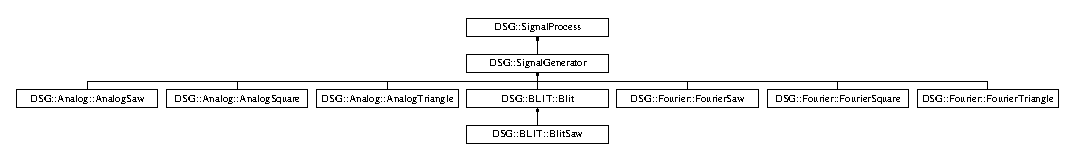
\includegraphics[height=1.702128cm]{class_d_s_g_1_1_signal_process}
\end{center}
\end{figure}
\subsection*{Public Member Functions}
\begin{DoxyCompactItemize}
\item 
\hypertarget{class_d_s_g_1_1_signal_process_af73d246c460915db7a9be7e3ef36844d}{virtual bool {\bfseries Perform} (D\+S\+G\+::\+D\+S\+G\+Sample \&signal)=0}\label{class_d_s_g_1_1_signal_process_af73d246c460915db7a9be7e3ef36844d}

\item 
\hypertarget{class_d_s_g_1_1_signal_process_a2c8ff3487d9c43f9eace1d9192d4a37e}{virtual bool {\bfseries Perform} (\hyperlink{class_d_s_g_1_1_ring_buffer}{D\+S\+G\+::\+Ring\+Buffer} \&signal)=0}\label{class_d_s_g_1_1_signal_process_a2c8ff3487d9c43f9eace1d9192d4a37e}

\end{DoxyCompactItemize}


\subsection{Detailed Description}
\hyperlink{class_d_s_g_1_1_signal_process}{D\+S\+G\+::\+Signal\+Process} -\/ Defines Base Interface For Audio Processing. 

The documentation for this class was generated from the following files\+:\begin{DoxyCompactItemize}
\item 
/\+Users/alexanderzywicki/\+Documents/\+D\+S\+G/src/Signal\+Process.\+h\item 
/\+Users/alexanderzywicki/\+Documents/\+D\+S\+G/src/Signal\+Process.\+cpp\end{DoxyCompactItemize}

\chapter{File Documentation}
\hypertarget{_analog_saw_8cpp}{\section{/\+Users/alexanderzywicki/\+Documents/\+D\+S\+G/src/\+Analog\+Saw.cpp File Reference}
\label{_analog_saw_8cpp}\index{/\+Users/alexanderzywicki/\+Documents/\+D\+S\+G/src/\+Analog\+Saw.\+cpp@{/\+Users/alexanderzywicki/\+Documents/\+D\+S\+G/src/\+Analog\+Saw.\+cpp}}
}
{\ttfamily \#include \char`\"{}Analog\+Saw.\+h\char`\"{}}\\*

\hypertarget{_analog_saw_8cpp_source}{\section{Analog\+Saw.\+cpp}
\label{_analog_saw_8cpp_source}\index{Analog\+Saw.\+cpp@{Analog\+Saw.\+cpp}}
}

\begin{DoxyCode}
00001 \textcolor{comment}{//}
00002 \textcolor{comment}{//  AnalogSaw.cpp}
00003 \textcolor{comment}{//  DSG}
00004 \textcolor{comment}{//}
00005 \textcolor{comment}{//  Created by Alexander Zywicki on 9/17/14.}
00006 \textcolor{comment}{//  Copyright (c) 2014 Alexander Zywicki. All rights reserved.}
00007 \textcolor{comment}{//}
00008 \textcolor{comment}{/*}
00009 \textcolor{comment}{ This file is part of the Digital Signal Generation Project or “DSG”.}
00010 \textcolor{comment}{}
00011 \textcolor{comment}{ DSG is free software: you can redistribute it and/or modify}
00012 \textcolor{comment}{ it under the terms of the GNU Lesser General Public License as published by}
00013 \textcolor{comment}{ the Free Software Foundation, either version 3 of the License, or}
00014 \textcolor{comment}{ (at your option) any later version.}
00015 \textcolor{comment}{}
00016 \textcolor{comment}{ DSG is distributed in the hope that it will be useful,}
00017 \textcolor{comment}{ but WITHOUT ANY WARRANTY; without even the implied warranty of}
00018 \textcolor{comment}{ MERCHANTABILITY or FITNESS FOR A PARTICULAR PURPOSE.  See the}
00019 \textcolor{comment}{ GNU Lesser General Public License for more details.}
00020 \textcolor{comment}{}
00021 \textcolor{comment}{ You should have received a copy of the GNU Lesser General Public License}
00022 \textcolor{comment}{ along with DSG.  If not, see <http://www.gnu.org/licenses/>.}
00023 \textcolor{comment}{ */}
00024 \textcolor{preprocessor}{#include "\hyperlink{_analog_saw_8h}{AnalogSaw.h}"}
\hypertarget{_analog_saw_8cpp_source_l00025}{}\hyperlink{class_d_s_g_1_1_analog_1_1_analog_saw_abcb0b997be32413da0d14b93aeeb9c17}{00025} \hyperlink{class_d_s_g_1_1_analog_1_1_analog_saw_abcb0b997be32413da0d14b93aeeb9c17}{DSG::Analog::AnalogSaw::AnalogSaw}():\hyperlink{namespace_d_s_g}{DSG}::
      \hyperlink{class_d_s_g_1_1_signal_generator}{SignalGenerator}()\{\}
\hypertarget{_analog_saw_8cpp_source_l00026}{}\hyperlink{class_d_s_g_1_1_analog_1_1_analog_saw_ad110da0b337948fb70ecdfad7dbb5ddf}{00026} \hyperlink{class_d_s_g_1_1_analog_1_1_analog_saw_abcb0b997be32413da0d14b93aeeb9c17}{DSG::Analog::AnalogSaw::AnalogSaw}(
      \hyperlink{namespace_d_s_g_a4315a061386fa1014fda09b15d3a6973}{DSG::DSGFrequency} \textcolor{keyword}{const}& frequency,\hyperlink{namespace_d_s_g_a44431ce1eb0a7300efdd207bc879e52c}{DSG::DSGPhase} \textcolor{keyword}{const}& offset):
      \hyperlink{namespace_d_s_g}{DSG}::\hyperlink{class_d_s_g_1_1_signal_generator}{SignalGenerator}(frequency,offset)\{\}
\hypertarget{_analog_saw_8cpp_source_l00027}{}\hyperlink{class_d_s_g_1_1_analog_1_1_analog_saw_a42a5fe22e0c3b9d1bd3996fe5bbd24ba}{00027} \hyperlink{class_d_s_g_1_1_analog_1_1_analog_saw_a42a5fe22e0c3b9d1bd3996fe5bbd24ba}{DSG::Analog::AnalogSaw::~AnalogSaw}()\{\}
\end{DoxyCode}

\hypertarget{_analog_saw_8h}{\section{/\+Users/alexanderzywicki/\+Documents/\+D\+S\+G/src/\+Analog\+Saw.h File Reference}
\label{_analog_saw_8h}\index{/\+Users/alexanderzywicki/\+Documents/\+D\+S\+G/src/\+Analog\+Saw.\+h@{/\+Users/alexanderzywicki/\+Documents/\+D\+S\+G/src/\+Analog\+Saw.\+h}}
}
{\ttfamily \#include \char`\"{}Signal\+Generator.\+h\char`\"{}}\\*
\subsection*{Classes}
\begin{DoxyCompactItemize}
\item 
class \hyperlink{class_d_s_g_1_1_analog_1_1_analog_saw}{D\+S\+G\+::\+Analog\+::\+Analog\+Saw}
\begin{DoxyCompactList}\small\item\em \hyperlink{class_d_s_g_1_1_analog_1_1_analog_saw}{D\+S\+G\+::\+Analog\+::\+Analog\+Saw} -\/ \hyperlink{namespace_d_s_g_1_1_analog}{Analog} Syle Saw Wave Generator. \end{DoxyCompactList}\end{DoxyCompactItemize}
\subsection*{Namespaces}
\begin{DoxyCompactItemize}
\item 
 \hyperlink{namespace_d_s_g}{D\+S\+G}
\begin{DoxyCompactList}\small\item\em \hyperlink{namespace_d_s_g}{D\+S\+G} -\/ A Collection of tools for Digital Signal Generation. \end{DoxyCompactList}\item 
 \hyperlink{namespace_d_s_g_1_1_analog}{D\+S\+G\+::\+Analog}
\begin{DoxyCompactList}\small\item\em \hyperlink{namespace_d_s_g_1_1_analog}{D\+S\+G\+::\+Analog} -\/ Namespace Containing \hyperlink{namespace_d_s_g_1_1_analog}{Analog} Style Oscillators. \end{DoxyCompactList}\end{DoxyCompactItemize}

\hypertarget{_analog_saw_8h_source}{\section{Analog\+Saw.\+h}
\label{_analog_saw_8h_source}\index{Analog\+Saw.\+h@{Analog\+Saw.\+h}}
}

\begin{DoxyCode}
00001 \textcolor{comment}{//}
00002 \textcolor{comment}{//  AnalogSaw.h}
00003 \textcolor{comment}{//  DSG}
00004 \textcolor{comment}{//}
00005 \textcolor{comment}{//  Created by Alexander Zywicki on 9/17/14.}
00006 \textcolor{comment}{//  Copyright (c) 2014 Alexander Zywicki. All rights reserved.}
00007 \textcolor{comment}{//}
00008 \textcolor{comment}{/*}
00009 \textcolor{comment}{ This file is part of the Digital Signal Generation Project or “DSG”.}
00010 \textcolor{comment}{}
00011 \textcolor{comment}{ DSG is free software: you can redistribute it and/or modify}
00012 \textcolor{comment}{ it under the terms of the GNU General Public License as published by}
00013 \textcolor{comment}{ the Free Software Foundation, either version 3 of the License, or}
00014 \textcolor{comment}{ (at your option) any later version.}
00015 \textcolor{comment}{}
00016 \textcolor{comment}{ DSG is distributed in the hope that it will be useful,}
00017 \textcolor{comment}{ but WITHOUT ANY WARRANTY; without even the implied warranty of}
00018 \textcolor{comment}{ MERCHANTABILITY or FITNESS FOR A PARTICULAR PURPOSE.  See the}
00019 \textcolor{comment}{ GNU General Public License for more details.}
00020 \textcolor{comment}{}
00021 \textcolor{comment}{ You should have received a copy of the GNU General Public License}
00022 \textcolor{comment}{ along with DSG.  If not, see <http://www.gnu.org/licenses/>.}
00023 \textcolor{comment}{ */}
00024 \textcolor{preprocessor}{#ifndef \_\_DSG\_\_AnalogSaw\_\_}
00025 \textcolor{preprocessor}{#define \_\_DSG\_\_AnalogSaw\_\_}
00026 \textcolor{preprocessor}{#include "\hyperlink{_signal_generator_8h}{SignalGenerator.h}"}
\hypertarget{_analog_saw_8h_source_l00027}{}\hyperlink{namespace_d_s_g}{00027} \textcolor{keyword}{namespace }\hyperlink{namespace_d_s_g}{DSG}\{
00028 \textcolor{preprocessor}{#ifdef DSG\_Short\_Names}
00029     \textcolor{keyword}{inline}
00030 \textcolor{preprocessor}{#endif}
00031 \textcolor{comment}{    //! DSG::Analog - Namespace Containing Analog Style Oscillators}
\hypertarget{_analog_saw_8h_source_l00032}{}\hyperlink{namespace_d_s_g_1_1_analog}{00032} \textcolor{comment}{}    \textcolor{keyword}{namespace }Analog\{\textcolor{comment}{}
00033 \textcolor{comment}{        //!\(\backslash\)brief DSG::Analog::AnalogSaw - Analog Syle Saw Wave Generator}
\hypertarget{_analog_saw_8h_source_l00034}{}\hyperlink{class_d_s_g_1_1_analog_1_1_analog_saw}{00034} \textcolor{comment}{}        \textcolor{keyword}{class }\hyperlink{class_d_s_g_1_1_analog_1_1_analog_saw}{AnalogSaw} : \textcolor{keyword}{public} \hyperlink{class_d_s_g_1_1_signal_generator}{DSG::SignalGenerator} \{
00035         \textcolor{keyword}{public}:
00036             \hyperlink{class_d_s_g_1_1_analog_1_1_analog_saw_abcb0b997be32413da0d14b93aeeb9c17}{AnalogSaw}();
00037             \hyperlink{class_d_s_g_1_1_analog_1_1_analog_saw_abcb0b997be32413da0d14b93aeeb9c17}{AnalogSaw}(\hyperlink{namespace_d_s_g_a4315a061386fa1014fda09b15d3a6973}{DSG::DSGFrequency} \textcolor{keyword}{const}& frequency,
      \hyperlink{namespace_d_s_g_a44431ce1eb0a7300efdd207bc879e52c}{DSG::DSGPhase} \textcolor{keyword}{const}& offset);
00038             \textcolor{keyword}{virtual} \hyperlink{class_d_s_g_1_1_analog_1_1_analog_saw_a42a5fe22e0c3b9d1bd3996fe5bbd24ba}{~AnalogSaw}();
00039             \textcolor{keyword}{virtual} \textcolor{keyword}{inline} \textcolor{keywordtype}{bool} \hyperlink{class_d_s_g_1_1_analog_1_1_analog_saw_a8d36e77c09ba84128e786c7bb14cddda}{Perform}(\hyperlink{namespace_d_s_g_ac39a94cd27ebcd9c1e7502d0c624894a}{DSG::DSGSample}& signal);
00040             \textcolor{keyword}{virtual} \textcolor{keyword}{inline} \textcolor{keywordtype}{bool} \hyperlink{class_d_s_g_1_1_analog_1_1_analog_saw_a8d36e77c09ba84128e786c7bb14cddda}{Perform}(\hyperlink{class_d_s_g_1_1_ring_buffer}{DSG::RingBuffer}& signal);
00041         \textcolor{keyword}{protected}:
\hypertarget{_analog_saw_8h_source_l00042}{}\hyperlink{class_d_s_g_1_1_analog_1_1_analog_saw_a81a923800bb8ba0f788d3567d2965d2a}{00042}             \hyperlink{namespace_d_s_g_ac39a94cd27ebcd9c1e7502d0c624894a}{DSG::DSGSample} \hyperlink{class_d_s_g_1_1_analog_1_1_analog_saw_a81a923800bb8ba0f788d3567d2965d2a}{\_stor};
00043         \};
\hypertarget{_analog_saw_8h_source_l00044}{}\hyperlink{class_d_s_g_1_1_analog_1_1_analog_saw_a8d36e77c09ba84128e786c7bb14cddda}{00044}         \textcolor{keyword}{inline} \textcolor{keywordtype}{bool} \hyperlink{class_d_s_g_1_1_analog_1_1_analog_saw_a8d36e77c09ba84128e786c7bb14cddda}{DSG::Analog::AnalogSaw::Perform}(
      \hyperlink{namespace_d_s_g_ac39a94cd27ebcd9c1e7502d0c624894a}{DSG::DSGSample}& signal)\{
00045             \_stor=\_phasor;
00046             \_stor+=0.5;
00047             \textcolor{keywordflow}{if} (\_stor>1.0) \{
00048                 --\_stor;
00049             \}
00050             \_stor-=0.5;
00051             \_stor*=2.0;
00052             signal=\_stor;
00053             step();
00054             \textcolor{keywordflow}{return} \textcolor{keyword}{true};
00055         \}
\hypertarget{_analog_saw_8h_source_l00056}{}\hyperlink{class_d_s_g_1_1_analog_1_1_analog_saw_a38f091059d924c9141fee3e27522e7e1}{00056}         \textcolor{keyword}{inline} \textcolor{keywordtype}{bool} \hyperlink{class_d_s_g_1_1_analog_1_1_analog_saw_a8d36e77c09ba84128e786c7bb14cddda}{DSG::Analog::AnalogSaw::Perform}(
      \hyperlink{class_d_s_g_1_1_ring_buffer}{DSG::RingBuffer}& signal)\{
00057             signal.\hyperlink{class_d_s_g_1_1_ring_buffer_ab23c8003d2857809a816068eeb209d60}{Flush}();
00058             \textcolor{keywordflow}{while} (!signal.\hyperlink{class_d_s_g_1_1_ring_buffer_a53ddb04ffcbb5470a8d2b0a3c65b70cb}{Full}()) \{
00059                 \textcolor{keywordflow}{if} (Perform(\_storage)) \{
00060                     \textcolor{keywordflow}{if}(signal.\hyperlink{class_d_s_g_1_1_ring_buffer_aa5dd2caa0a270173251faee40a43d692}{Write}(\_storage))\{
00061                     \}\textcolor{keywordflow}{else} \textcolor{keywordflow}{return} \textcolor{keyword}{false};
00062                 \}\textcolor{keywordflow}{else} \textcolor{keywordflow}{return} \textcolor{keyword}{false};
00063             \}\textcolor{keywordflow}{return} \textcolor{keyword}{true};
00064         \}
00065     \}
00066 \}
00067 \textcolor{preprocessor}{#endif }\textcolor{comment}{/* defined(\_\_DSG\_\_AnalogSaw\_\_) */}\textcolor{preprocessor}{}
\end{DoxyCode}

\hypertarget{_analog_square_8cpp}{\section{/\+Users/alexanderzywicki/\+Documents/\+D\+S\+G/src/\+Analog\+Square.cpp File Reference}
\label{_analog_square_8cpp}\index{/\+Users/alexanderzywicki/\+Documents/\+D\+S\+G/src/\+Analog\+Square.\+cpp@{/\+Users/alexanderzywicki/\+Documents/\+D\+S\+G/src/\+Analog\+Square.\+cpp}}
}
{\ttfamily \#include \char`\"{}Analog\+Square.\+h\char`\"{}}\\*

\hypertarget{_analog_square_8cpp_source}{\section{Analog\+Square.\+cpp}
\label{_analog_square_8cpp_source}\index{/\+Users/alexanderzywicki/\+Documents/\+D\+S\+G/src/\+Analog\+Square.\+cpp@{/\+Users/alexanderzywicki/\+Documents/\+D\+S\+G/src/\+Analog\+Square.\+cpp}}
}

\begin{DoxyCode}
00001 \textcolor{comment}{//}
00002 \textcolor{comment}{//  AnalogSquare.cpp}
00003 \textcolor{comment}{//  DSG}
00004 \textcolor{comment}{//}
00005 \textcolor{comment}{//  Created by Alexander Zywicki on 9/17/14.}
00006 \textcolor{comment}{//  Copyright (c) 2014 Alexander Zywicki. All rights reserved.}
00007 \textcolor{comment}{//}
00008 \textcolor{preprocessor}{#include "\hyperlink{_analog_square_8h}{AnalogSquare.h}"}
\hypertarget{_analog_square_8cpp_source_l00009}{}\hyperlink{class_d_s_g_1_1_analog_1_1_analog_square_a7425ebd7e39129178eb050a04cd9d5d6}{00009} \hyperlink{class_d_s_g_1_1_analog_1_1_analog_square_a7425ebd7e39129178eb050a04cd9d5d6}{DSG::Analog::AnalogSquare::AnalogSquare}():
      \hyperlink{namespace_d_s_g}{DSG}::\hyperlink{class_d_s_g_1_1_signal_generator}{SignalGenerator}()\{\}
\hypertarget{_analog_square_8cpp_source_l00010}{}\hyperlink{class_d_s_g_1_1_analog_1_1_analog_square_a886eb67edded43efca895741559a55f4}{00010} \hyperlink{class_d_s_g_1_1_analog_1_1_analog_square_a7425ebd7e39129178eb050a04cd9d5d6}{DSG::Analog::AnalogSquare::AnalogSquare}(
      \hyperlink{namespace_d_s_g_a4315a061386fa1014fda09b15d3a6973}{DSG::DSGFrequency} \textcolor{keyword}{const}& frequency,\hyperlink{namespace_d_s_g_a44431ce1eb0a7300efdd207bc879e52c}{DSG::DSGPhase} \textcolor{keyword}{const}& offset):
      \hyperlink{namespace_d_s_g}{DSG}::\hyperlink{class_d_s_g_1_1_signal_generator}{SignalGenerator}(frequency,offset)\{\}
\hypertarget{_analog_square_8cpp_source_l00011}{}\hyperlink{class_d_s_g_1_1_analog_1_1_analog_square_a17b3928f19cb6bf0c151b5e1159de1db}{00011} \hyperlink{class_d_s_g_1_1_analog_1_1_analog_square_a17b3928f19cb6bf0c151b5e1159de1db}{DSG::Analog::AnalogSquare::~AnalogSquare}()\{\}
\end{DoxyCode}

\hypertarget{_analog_square_8h}{\section{/\+Users/alexanderzywicki/\+Documents/\+D\+S\+G/src/\+Analog\+Square.h File Reference}
\label{_analog_square_8h}\index{/\+Users/alexanderzywicki/\+Documents/\+D\+S\+G/src/\+Analog\+Square.\+h@{/\+Users/alexanderzywicki/\+Documents/\+D\+S\+G/src/\+Analog\+Square.\+h}}
}
{\ttfamily \#include \char`\"{}Signal\+Generator.\+h\char`\"{}}\\*
\subsection*{Classes}
\begin{DoxyCompactItemize}
\item 
class \hyperlink{class_d_s_g_1_1_analog_1_1_analog_square}{D\+S\+G\+::\+Analog\+::\+Analog\+Square}
\begin{DoxyCompactList}\small\item\em \hyperlink{class_d_s_g_1_1_analog_1_1_analog_square}{D\+S\+G\+::\+Analog\+::\+Analog\+Square} -\/ \hyperlink{namespace_d_s_g_1_1_analog}{Analog} Syle Square Wave Generator. \end{DoxyCompactList}\end{DoxyCompactItemize}
\subsection*{Namespaces}
\begin{DoxyCompactItemize}
\item 
 \hyperlink{namespace_d_s_g}{D\+S\+G}
\begin{DoxyCompactList}\small\item\em \hyperlink{namespace_d_s_g}{D\+S\+G} -\/ A Collection of tools for Digital Signal Generation. \end{DoxyCompactList}\item 
 \hyperlink{namespace_d_s_g_1_1_analog}{D\+S\+G\+::\+Analog}
\begin{DoxyCompactList}\small\item\em \hyperlink{namespace_d_s_g_1_1_analog}{D\+S\+G\+::\+Analog} -\/ Namespace Containing \hyperlink{namespace_d_s_g_1_1_analog}{Analog} Style Oscillators. \end{DoxyCompactList}\end{DoxyCompactItemize}

\hypertarget{_analog_square_8h_source}{\section{Analog\+Square.\+h}
\label{_analog_square_8h_source}\index{/\+Users/alexanderzywicki/\+Documents/\+D\+S\+G/src/\+Analog\+Square.\+h@{/\+Users/alexanderzywicki/\+Documents/\+D\+S\+G/src/\+Analog\+Square.\+h}}
}

\begin{DoxyCode}
00001 \textcolor{comment}{//}
00002 \textcolor{comment}{//  AnalogSquare.h}
00003 \textcolor{comment}{//  DSG}
00004 \textcolor{comment}{//}
00005 \textcolor{comment}{//  Created by Alexander Zywicki on 9/17/14.}
00006 \textcolor{comment}{//  Copyright (c) 2014 Alexander Zywicki. All rights reserved.}
00007 \textcolor{comment}{//}
00008 \textcolor{preprocessor}{#ifndef \_\_DSG\_\_AnalogSquare\_\_}
00009 \textcolor{preprocessor}{#define \_\_DSG\_\_AnalogSquare\_\_}
00010 \textcolor{preprocessor}{#include "\hyperlink{_signal_generator_8h}{SignalGenerator.h}"}
00011 \textcolor{keyword}{namespace }\hyperlink{namespace_d_s_g}{DSG}\{
00012 \textcolor{preprocessor}{#ifdef DSG\_Short\_Names}
00013     \textcolor{keyword}{inline}
00014 \textcolor{preprocessor}{#endif}
00015 \textcolor{comment}{    //! DSG::Analog - Namespace Containing Analog Style Oscillators}
00016 \textcolor{comment}{}    \textcolor{keyword}{namespace }Analog\{\textcolor{comment}{}
00017 \textcolor{comment}{        //!\(\backslash\)brief DSG::Analog::AnalogSquare - Analog Syle Square Wave Generator}
\hypertarget{_analog_square_8h_source_l00018}{}\hyperlink{class_d_s_g_1_1_analog_1_1_analog_square}{00018} \textcolor{comment}{}        \textcolor{keyword}{class }\hyperlink{class_d_s_g_1_1_analog_1_1_analog_square}{AnalogSquare} : \textcolor{keyword}{public} \hyperlink{class_d_s_g_1_1_signal_generator}{DSG::SignalGenerator} \{
00019         \textcolor{keyword}{public}:
00020             \hyperlink{class_d_s_g_1_1_analog_1_1_analog_square_a7425ebd7e39129178eb050a04cd9d5d6}{AnalogSquare}();
00021             \hyperlink{class_d_s_g_1_1_analog_1_1_analog_square_a7425ebd7e39129178eb050a04cd9d5d6}{AnalogSquare}(\hyperlink{namespace_d_s_g_a4315a061386fa1014fda09b15d3a6973}{DSG::DSGFrequency} \textcolor{keyword}{const}& frequency,
      \hyperlink{namespace_d_s_g_a44431ce1eb0a7300efdd207bc879e52c}{DSG::DSGPhase} \textcolor{keyword}{const}& offset);
00022             \textcolor{keyword}{virtual} \hyperlink{class_d_s_g_1_1_analog_1_1_analog_square_a17b3928f19cb6bf0c151b5e1159de1db}{~AnalogSquare}();
00023             \textcolor{keyword}{virtual} \textcolor{keyword}{inline} \textcolor{keywordtype}{bool} \hyperlink{class_d_s_g_1_1_analog_1_1_analog_square_a784aa17d266704647789b972cf880e9f}{Perform}(\hyperlink{namespace_d_s_g_ac39a94cd27ebcd9c1e7502d0c624894a}{DSG::DSGSample}& signal);
00024             \textcolor{keyword}{virtual} \textcolor{keyword}{inline} \textcolor{keywordtype}{bool} \hyperlink{class_d_s_g_1_1_analog_1_1_analog_square_a784aa17d266704647789b972cf880e9f}{Perform}(\hyperlink{class_d_s_g_1_1_ring_buffer}{DSG::RingBuffer}& signal);
00025         \};
\hypertarget{_analog_square_8h_source_l00026}{}\hyperlink{class_d_s_g_1_1_analog_1_1_analog_square_a784aa17d266704647789b972cf880e9f}{00026}         \textcolor{keyword}{inline} \textcolor{keywordtype}{bool} \hyperlink{class_d_s_g_1_1_analog_1_1_analog_square_a784aa17d266704647789b972cf880e9f}{DSG::Analog::AnalogSquare::Perform}(
      \hyperlink{namespace_d_s_g_ac39a94cd27ebcd9c1e7502d0c624894a}{DSG::DSGSample}& signal)\{
00027             signal=\_phasor < 0.5 ? 1.0:-1.0;
00028             step();
00029             \textcolor{keywordflow}{return} \textcolor{keyword}{true};
00030         \}
\hypertarget{_analog_square_8h_source_l00031}{}\hyperlink{class_d_s_g_1_1_analog_1_1_analog_square_af4d41d5894ae02e920c61e06cf041c60}{00031}         \textcolor{keyword}{inline} \textcolor{keywordtype}{bool} \hyperlink{class_d_s_g_1_1_analog_1_1_analog_square_a784aa17d266704647789b972cf880e9f}{DSG::Analog::AnalogSquare::Perform}(
      \hyperlink{class_d_s_g_1_1_ring_buffer}{DSG::RingBuffer}& signal)\{
00032             signal.\hyperlink{class_d_s_g_1_1_ring_buffer_ab23c8003d2857809a816068eeb209d60}{Flush}();
00033             \textcolor{keywordflow}{while} (!signal.\hyperlink{class_d_s_g_1_1_ring_buffer_a53ddb04ffcbb5470a8d2b0a3c65b70cb}{Full}()) \{
00034                 \textcolor{keywordflow}{if} (Perform(\_storage)) \{
00035                     \textcolor{keywordflow}{if}(signal.\hyperlink{class_d_s_g_1_1_ring_buffer_aa5dd2caa0a270173251faee40a43d692}{Write}(\_storage))\{
00036                     \}\textcolor{keywordflow}{else} \textcolor{keywordflow}{return} \textcolor{keyword}{false};
00037                 \}\textcolor{keywordflow}{else} \textcolor{keywordflow}{return} \textcolor{keyword}{false};
00038             \}\textcolor{keywordflow}{return} \textcolor{keyword}{true};
00039         \}
00040     \}
00041 \}
00042 \textcolor{preprocessor}{#endif }\textcolor{comment}{/* defined(\_\_DSG\_\_AnalogSquare\_\_) */}\textcolor{preprocessor}{}
\end{DoxyCode}

\hypertarget{_analog_triangle_8cpp}{\section{Analog\+Triangle.\+cpp File Reference}
\label{_analog_triangle_8cpp}\index{Analog\+Triangle.\+cpp@{Analog\+Triangle.\+cpp}}
}
{\ttfamily \#include \char`\"{}Analog\+Triangle.\+h\char`\"{}}\\*

\hypertarget{_analog_triangle_8cpp_source}{\section{Analog\+Triangle.\+cpp}
\label{_analog_triangle_8cpp_source}\index{Analog\+Triangle.\+cpp@{Analog\+Triangle.\+cpp}}
}

\begin{DoxyCode}
00001 \textcolor{comment}{//}
00002 \textcolor{comment}{//  AnalogTriangle.cpp}
00003 \textcolor{comment}{//  DSG}
00004 \textcolor{comment}{//}
00005 \textcolor{comment}{//  Created by Alexander Zywicki on 9/17/14.}
00006 \textcolor{comment}{//  Copyright (c) 2014 Alexander Zywicki. All rights reserved.}
00007 \textcolor{comment}{//}
00008 \textcolor{comment}{/*}
00009 \textcolor{comment}{ This file is part of the Digital Signal Generation Project or “DSG”.}
00010 \textcolor{comment}{}
00011 \textcolor{comment}{ DSG is free software: you can redistribute it and/or modify}
00012 \textcolor{comment}{ it under the terms of the GNU General Public License as published by}
00013 \textcolor{comment}{ the Free Software Foundation, either version 3 of the License, or}
00014 \textcolor{comment}{ (at your option) any later version.}
00015 \textcolor{comment}{}
00016 \textcolor{comment}{ DSG is distributed in the hope that it will be useful,}
00017 \textcolor{comment}{ but WITHOUT ANY WARRANTY; without even the implied warranty of}
00018 \textcolor{comment}{ MERCHANTABILITY or FITNESS FOR A PARTICULAR PURPOSE.  See the}
00019 \textcolor{comment}{ GNU General Public License for more details.}
00020 \textcolor{comment}{}
00021 \textcolor{comment}{ You should have received a copy of the GNU General Public License}
00022 \textcolor{comment}{ along with DSG.  If not, see <http://www.gnu.org/licenses/>.}
00023 \textcolor{comment}{ */}
00024 \textcolor{preprocessor}{#include "\hyperlink{_analog_triangle_8h}{AnalogTriangle.h}"}
\hypertarget{_analog_triangle_8cpp_source_l00025}{}\hyperlink{class_d_s_g_1_1_analog_1_1_analog_triangle_a2fe1a7a29eb9472323a2a1c0d0696e55}{00025} \hyperlink{class_d_s_g_1_1_analog_1_1_analog_triangle_a2fe1a7a29eb9472323a2a1c0d0696e55}{DSG::Analog::AnalogTriangle::AnalogTriangle}():
      \hyperlink{namespace_d_s_g}{DSG}::\hyperlink{class_d_s_g_1_1_signal_generator}{SignalGenerator}()\{\}
\hypertarget{_analog_triangle_8cpp_source_l00026}{}\hyperlink{class_d_s_g_1_1_analog_1_1_analog_triangle_a75c0a8b20e1843b35de3944da11c75ed}{00026} \hyperlink{class_d_s_g_1_1_analog_1_1_analog_triangle_a2fe1a7a29eb9472323a2a1c0d0696e55}{DSG::Analog::AnalogTriangle::AnalogTriangle}(
      \hyperlink{namespace_d_s_g_a4315a061386fa1014fda09b15d3a6973}{DSG::DSGFrequency} \textcolor{keyword}{const}& frequency,\hyperlink{namespace_d_s_g_a44431ce1eb0a7300efdd207bc879e52c}{DSG::DSGPhase} \textcolor{keyword}{const}& offset):
      \hyperlink{namespace_d_s_g}{DSG}::\hyperlink{class_d_s_g_1_1_signal_generator}{SignalGenerator}(frequency,offset)\{\}
\hypertarget{_analog_triangle_8cpp_source_l00027}{}\hyperlink{class_d_s_g_1_1_analog_1_1_analog_triangle_af6e127d2fb623afad9b172e7c8b3c656}{00027} \hyperlink{class_d_s_g_1_1_analog_1_1_analog_triangle_af6e127d2fb623afad9b172e7c8b3c656}{DSG::Analog::AnalogTriangle::~AnalogTriangle}()\{\}
\end{DoxyCode}

\hypertarget{_analog_triangle_8h}{\section{Analog\+Triangle.\+h File Reference}
\label{_analog_triangle_8h}\index{Analog\+Triangle.\+h@{Analog\+Triangle.\+h}}
}
{\ttfamily \#include \char`\"{}Signal\+Generator.\+h\char`\"{}}\\*
\subsection*{Classes}
\begin{DoxyCompactItemize}
\item 
class \hyperlink{class_d_s_g_1_1_analog_1_1_analog_triangle}{D\+S\+G\+::\+Analog\+::\+Analog\+Triangle}
\begin{DoxyCompactList}\small\item\em \hyperlink{class_d_s_g_1_1_analog_1_1_analog_triangle}{D\+S\+G\+::\+Analog\+::\+Analog\+Triangle} -\/ \hyperlink{namespace_d_s_g_1_1_analog}{Analog} Syle Triangle Wave Generator. \end{DoxyCompactList}\end{DoxyCompactItemize}
\subsection*{Namespaces}
\begin{DoxyCompactItemize}
\item 
 \hyperlink{namespace_d_s_g}{D\+S\+G}
\begin{DoxyCompactList}\small\item\em \hyperlink{namespace_d_s_g}{D\+S\+G} -\/ A Collection of tools for Digital Signal Generation. \end{DoxyCompactList}\item 
 \hyperlink{namespace_d_s_g_1_1_analog}{D\+S\+G\+::\+Analog}
\begin{DoxyCompactList}\small\item\em \hyperlink{namespace_d_s_g_1_1_analog}{D\+S\+G\+::\+Analog} -\/ Namespace Containing \hyperlink{namespace_d_s_g_1_1_analog}{Analog} Style Oscillators. \end{DoxyCompactList}\end{DoxyCompactItemize}

\hypertarget{_analog_triangle_8h_source}{\section{Analog\+Triangle.\+h}
\label{_analog_triangle_8h_source}\index{/\+Users/alexanderzywicki/\+Documents/\+D\+S\+G/src/\+Analog\+Triangle.\+h@{/\+Users/alexanderzywicki/\+Documents/\+D\+S\+G/src/\+Analog\+Triangle.\+h}}
}

\begin{DoxyCode}
00001 \textcolor{comment}{//}
00002 \textcolor{comment}{//  AnalogTriangle.h}
00003 \textcolor{comment}{//  DSG}
00004 \textcolor{comment}{//}
00005 \textcolor{comment}{//  Created by Alexander Zywicki on 9/17/14.}
00006 \textcolor{comment}{//  Copyright (c) 2014 Alexander Zywicki. All rights reserved.}
00007 \textcolor{comment}{//}
00008 \textcolor{preprocessor}{#ifndef \_\_DSG\_\_AnalogTriangle\_\_}
00009 \textcolor{preprocessor}{#define \_\_DSG\_\_AnalogTriangle\_\_}
00010 \textcolor{preprocessor}{#include "\hyperlink{_signal_generator_8h}{SignalGenerator.h}"}
00011 \textcolor{keyword}{namespace }\hyperlink{namespace_d_s_g}{DSG}\{
00012 \textcolor{preprocessor}{#ifdef DSG\_Short\_Names}
00013     \textcolor{keyword}{inline}
00014 \textcolor{preprocessor}{#endif}
00015 \textcolor{comment}{    //! DSG::Analog - Namespace Containing Analog Style Oscillators}
00016 \textcolor{comment}{}    \textcolor{keyword}{namespace }Analog\{\textcolor{comment}{}
00017 \textcolor{comment}{        //!\(\backslash\)brief DSG::Analog::AnalogTriangle - Analog Syle Triangle Wave Generator}
\hypertarget{_analog_triangle_8h_source_l00018}{}\hyperlink{class_d_s_g_1_1_analog_1_1_analog_triangle}{00018} \textcolor{comment}{}        \textcolor{keyword}{class }\hyperlink{class_d_s_g_1_1_analog_1_1_analog_triangle}{AnalogTriangle} : \textcolor{keyword}{public} \hyperlink{class_d_s_g_1_1_signal_generator}{DSG::SignalGenerator} \{
00019         \textcolor{keyword}{public}:
00020             \hyperlink{class_d_s_g_1_1_analog_1_1_analog_triangle_a2fe1a7a29eb9472323a2a1c0d0696e55}{AnalogTriangle}();
00021             \hyperlink{class_d_s_g_1_1_analog_1_1_analog_triangle_a2fe1a7a29eb9472323a2a1c0d0696e55}{AnalogTriangle}(\hyperlink{namespace_d_s_g_a4315a061386fa1014fda09b15d3a6973}{DSG::DSGFrequency} \textcolor{keyword}{const}& frequency,
      \hyperlink{namespace_d_s_g_a44431ce1eb0a7300efdd207bc879e52c}{DSG::DSGPhase} \textcolor{keyword}{const}& offset);
00022             \textcolor{keyword}{virtual} \hyperlink{class_d_s_g_1_1_analog_1_1_analog_triangle_af6e127d2fb623afad9b172e7c8b3c656}{~AnalogTriangle}();
00023             \textcolor{keyword}{virtual} \textcolor{keyword}{inline} \textcolor{keywordtype}{bool} \hyperlink{class_d_s_g_1_1_analog_1_1_analog_triangle_a9b2484f3eb4c4ad545cb88b8833be124}{Perform}(\hyperlink{namespace_d_s_g_ac39a94cd27ebcd9c1e7502d0c624894a}{DSG::DSGSample}& signal);
00024             \textcolor{keyword}{virtual} \textcolor{keyword}{inline} \textcolor{keywordtype}{bool} \hyperlink{class_d_s_g_1_1_analog_1_1_analog_triangle_a9b2484f3eb4c4ad545cb88b8833be124}{Perform}(\hyperlink{class_d_s_g_1_1_ring_buffer}{DSG::RingBuffer}& signal);
00025         \textcolor{keyword}{protected}:
\hypertarget{_analog_triangle_8h_source_l00026}{}\hyperlink{class_d_s_g_1_1_analog_1_1_analog_triangle_ac93bccb7e366491f45ea9c3af04072ae}{00026}             \hyperlink{namespace_d_s_g_ac39a94cd27ebcd9c1e7502d0c624894a}{DSG::DSGSample} \hyperlink{class_d_s_g_1_1_analog_1_1_analog_triangle_ac93bccb7e366491f45ea9c3af04072ae}{\_stor};
00027         \};
\hypertarget{_analog_triangle_8h_source_l00028}{}\hyperlink{class_d_s_g_1_1_analog_1_1_analog_triangle_a9b2484f3eb4c4ad545cb88b8833be124}{00028}         \textcolor{keyword}{inline} \textcolor{keywordtype}{bool} \hyperlink{class_d_s_g_1_1_analog_1_1_analog_triangle_a9b2484f3eb4c4ad545cb88b8833be124}{DSG::Analog::AnalogTriangle::Perform}(
      \hyperlink{namespace_d_s_g_ac39a94cd27ebcd9c1e7502d0c624894a}{DSG::DSGSample}& signal)\{
00029             \_stor = \_phasor;
00030             \_stor+=0.25;
00031             \textcolor{keywordflow}{while} (\_stor>1.0) \{
00032                 \_stor-=1.0;
00033             \}
00034             \_stor-=0.5;
00035             \textcolor{keywordflow}{if} (\_stor<0) \{
00036                 \_stor*=-1.0;
00037             \}
00038             \_stor-=0.25;
00039             \_stor*=-4.0;
00040             signal = \_stor;
00041             step();\textcolor{comment}{//always last}
00042             \textcolor{keywordflow}{return} \textcolor{keyword}{true};
00043         \}
\hypertarget{_analog_triangle_8h_source_l00044}{}\hyperlink{class_d_s_g_1_1_analog_1_1_analog_triangle_a568c994e0f83f6a01d813357259a8f37}{00044}         \textcolor{keyword}{inline} \textcolor{keywordtype}{bool} \hyperlink{class_d_s_g_1_1_analog_1_1_analog_triangle_a9b2484f3eb4c4ad545cb88b8833be124}{DSG::Analog::AnalogTriangle::Perform}(
      \hyperlink{class_d_s_g_1_1_ring_buffer}{DSG::RingBuffer}& signal)\{
00045             signal.\hyperlink{class_d_s_g_1_1_ring_buffer_ab23c8003d2857809a816068eeb209d60}{Flush}();
00046             \textcolor{keywordflow}{while} (!signal.\hyperlink{class_d_s_g_1_1_ring_buffer_a53ddb04ffcbb5470a8d2b0a3c65b70cb}{Full}()) \{
00047                 \textcolor{keywordflow}{if} (Perform(\_storage)) \{
00048                     \textcolor{keywordflow}{if}(signal.\hyperlink{class_d_s_g_1_1_ring_buffer_aa5dd2caa0a270173251faee40a43d692}{Write}(\_storage))\{
00049                     \}\textcolor{keywordflow}{else} \textcolor{keywordflow}{return} \textcolor{keyword}{false};
00050                 \}\textcolor{keywordflow}{else} \textcolor{keywordflow}{return} \textcolor{keyword}{false};
00051             \}\textcolor{keywordflow}{return} \textcolor{keyword}{true};
00052         \}
00053     \}
00054 \} 
00055 \textcolor{preprocessor}{#endif }\textcolor{comment}{/* defined(\_\_DSG\_\_AnalogTriangle\_\_) */}\textcolor{preprocessor}{}
\end{DoxyCode}

\hypertarget{_audio_settings_8cpp}{\section{/\+Users/alexanderzywicki/\+Documents/\+D\+S\+G/src/\+Audio\+Settings.cpp File Reference}
\label{_audio_settings_8cpp}\index{/\+Users/alexanderzywicki/\+Documents/\+D\+S\+G/src/\+Audio\+Settings.\+cpp@{/\+Users/alexanderzywicki/\+Documents/\+D\+S\+G/src/\+Audio\+Settings.\+cpp}}
}
{\ttfamily \#include \char`\"{}Audio\+Settings.\+h\char`\"{}}\\*

\hypertarget{_audio_settings_8cpp_source}{\section{Audio\+Settings.\+cpp}
\label{_audio_settings_8cpp_source}\index{/\+Users/alexanderzywicki/\+Documents/\+D\+S\+G/src/\+Audio\+Settings.\+cpp@{/\+Users/alexanderzywicki/\+Documents/\+D\+S\+G/src/\+Audio\+Settings.\+cpp}}
}

\begin{DoxyCode}
00001 \textcolor{comment}{//}
00002 \textcolor{comment}{//  AudioSettings.cpp}
00003 \textcolor{comment}{//  DSG}
00004 \textcolor{comment}{//}
00005 \textcolor{comment}{//  Created by Alexander Zywicki on 9/16/14.}
00006 \textcolor{comment}{//  Copyright (c) 2014 Alexander Zywicki. All rights reserved.}
00007 \textcolor{comment}{//}
00008 \textcolor{preprocessor}{#include "\hyperlink{_audio_settings_8h}{AudioSettings.h}"}
00009 \hyperlink{namespace_d_s_g_a4315a061386fa1014fda09b15d3a6973}{DSG::DSGFrequency} \hyperlink{class_d_s_g_1_1_audio_settings_a56869b51933f102b197f54001c8a1d27}{DSG::AudioSettings::\_sampleRate};
00010 \hyperlink{namespace_d_s_g_a4315a061386fa1014fda09b15d3a6973}{DSG::DSGFrequency} \hyperlink{class_d_s_g_1_1_audio_settings_af3c7cbd15390d9bcbe39983c069390b5}{DSG::AudioSettings::\_nyquist};
\hypertarget{_audio_settings_8cpp_source_l00011}{}\hyperlink{class_d_s_g_1_1_audio_settings_a4f459c389b10c11828e2f2f00c012c49}{00011} \hyperlink{namespace_d_s_g_a4315a061386fa1014fda09b15d3a6973}{DSG::DSGFrequency} \textcolor{keyword}{const}& \hyperlink{class_d_s_g_1_1_audio_settings_a4f459c389b10c11828e2f2f00c012c49}{DSG::AudioSettings::SampleRate}()\{
00012     \textcolor{keywordflow}{return} \hyperlink{class_d_s_g_1_1_audio_settings_a56869b51933f102b197f54001c8a1d27}{\_sampleRate};
00013 \}
\hypertarget{_audio_settings_8cpp_source_l00014}{}\hyperlink{class_d_s_g_1_1_audio_settings_a9c5640e47b6eaa4331a0e5053abb1314}{00014} \hyperlink{namespace_d_s_g_a4315a061386fa1014fda09b15d3a6973}{DSG::DSGFrequency} \textcolor{keyword}{const}& \hyperlink{class_d_s_g_1_1_audio_settings_a4f459c389b10c11828e2f2f00c012c49}{DSG::AudioSettings::SampleRate}(
      \hyperlink{namespace_d_s_g_a4315a061386fa1014fda09b15d3a6973}{DSG::DSGFrequency} \textcolor{keyword}{const}& value)\{
00015     \_sampleRate = value;
00016     \_nyquist = \_sampleRate*0.5;
00017     \textcolor{keywordflow}{return} \_sampleRate;
00018 \}
\hypertarget{_audio_settings_8cpp_source_l00019}{}\hyperlink{class_d_s_g_1_1_audio_settings_a8cb4afd7b58e927300ff46fbeb71bec7}{00019} \hyperlink{namespace_d_s_g_a4315a061386fa1014fda09b15d3a6973}{DSG::DSGFrequency} \textcolor{keyword}{const}& \hyperlink{class_d_s_g_1_1_audio_settings_a8cb4afd7b58e927300ff46fbeb71bec7}{DSG::AudioSettings::Nyquist}()\{
00020     \textcolor{keywordflow}{return} \_nyquist;
00021 \}
\end{DoxyCode}

\hypertarget{_audio_settings_8h}{\section{Audio\+Settings.\+h File Reference}
\label{_audio_settings_8h}\index{Audio\+Settings.\+h@{Audio\+Settings.\+h}}
}
{\ttfamily \#include \char`\"{}D\+S\+G\+Types.\+h\char`\"{}}\\*
{\ttfamily \#include $<$vector$>$}\\*
\subsection*{Classes}
\begin{DoxyCompactItemize}
\item 
class \hyperlink{class_d_s_g_1_1_audio_settings}{D\+S\+G\+::\+Audio\+Settings}
\begin{DoxyCompactList}\small\item\em \hyperlink{class_d_s_g_1_1_audio_settings}{D\+S\+G\+::\+Audio\+Settings} -\/ Global Storage For Audio Settings Such As Sample Rate. \end{DoxyCompactList}\end{DoxyCompactItemize}
\subsection*{Namespaces}
\begin{DoxyCompactItemize}
\item 
 \hyperlink{namespace_d_s_g}{D\+S\+G}
\begin{DoxyCompactList}\small\item\em \hyperlink{namespace_d_s_g}{D\+S\+G} -\/ A Collection of tools for Digital Signal Generation. \end{DoxyCompactList}\end{DoxyCompactItemize}
\subsection*{Macros}
\begin{DoxyCompactItemize}
\item 
\#define \hyperlink{_audio_settings_8h_ad9d89453f9b7b69bd9beb58946863dd4}{Sample\+Rate\+Default}~44100
\end{DoxyCompactItemize}
\subsection*{Functions}
\begin{DoxyCompactItemize}
\item 
\hyperlink{namespace_d_s_g_a4315a061386fa1014fda09b15d3a6973}{D\+S\+G\+::\+D\+S\+G\+Frequency} const \& \hyperlink{namespace_d_s_g_a72df05177db0412c3590070923f62819}{D\+S\+G\+::\+Sample\+Rate} ()
\begin{DoxyCompactList}\small\item\em \hyperlink{namespace_d_s_g_a72df05177db0412c3590070923f62819}{D\+S\+G\+::\+Sample\+Rate} -\/ Get Global Sample Rate. \end{DoxyCompactList}\item 
\hyperlink{namespace_d_s_g_a4315a061386fa1014fda09b15d3a6973}{D\+S\+G\+::\+D\+S\+G\+Frequency} const \& \hyperlink{namespace_d_s_g_a66a464f016da1a099abea61a27a84d18}{D\+S\+G\+::\+Sample\+Rate} (\hyperlink{namespace_d_s_g_a4315a061386fa1014fda09b15d3a6973}{D\+S\+G\+::\+D\+S\+G\+Frequency} const \&value)
\begin{DoxyCompactList}\small\item\em \hyperlink{namespace_d_s_g_a72df05177db0412c3590070923f62819}{D\+S\+G\+::\+Sample\+Rate} -\/ Set Global Sample Rate. \end{DoxyCompactList}\item 
\hyperlink{namespace_d_s_g_a4315a061386fa1014fda09b15d3a6973}{D\+S\+G\+::\+D\+S\+G\+Frequency} \hyperlink{namespace_d_s_g_acb23c320b74d21f203081a25e1b5d134}{D\+S\+G\+::\+Nyquist} ()
\begin{DoxyCompactList}\small\item\em \hyperlink{namespace_d_s_g_acb23c320b74d21f203081a25e1b5d134}{D\+S\+G\+::\+Nyquist()} -\/ Pre-\/\+Calculated Nyquist Limit. Use instead of calculating each time needed. This value will be updated whenever the sample rate changes. \end{DoxyCompactList}\item 
bool \hyperlink{namespace_d_s_g_a66af6119635fe556dc5f840bf78dec56}{D\+S\+G\+::\+Add\+Sample\+Rate\+Listener} (\hyperlink{class_d_s_g_1_1_signal_process}{D\+S\+G\+::\+Signal\+Process} $\ast$listner)
\begin{DoxyCompactList}\small\item\em \hyperlink{namespace_d_s_g_a66af6119635fe556dc5f840bf78dec56}{D\+S\+G\+::\+Add\+Sample\+Rate\+Listener()} -\/ Allows Generators to be notified if the sample rate changes. \end{DoxyCompactList}\item 
void \hyperlink{namespace_d_s_g_a0749755eb0ed01894adc60fab768dfa5}{D\+S\+G\+::\+Verify\+Sample\+Rate\+Set} ()
\begin{DoxyCompactList}\small\item\em \hyperlink{namespace_d_s_g_a0749755eb0ed01894adc60fab768dfa5}{D\+S\+G\+::\+Verify\+Sample\+Rate\+Set()} -\/ Allows a Generator to ask if a valid sample rate has been set. \end{DoxyCompactList}\end{DoxyCompactItemize}


\subsection{Macro Definition Documentation}
\hypertarget{_audio_settings_8h_ad9d89453f9b7b69bd9beb58946863dd4}{\index{Audio\+Settings.\+h@{Audio\+Settings.\+h}!Sample\+Rate\+Default@{Sample\+Rate\+Default}}
\index{Sample\+Rate\+Default@{Sample\+Rate\+Default}!Audio\+Settings.\+h@{Audio\+Settings.\+h}}
\subsubsection[{Sample\+Rate\+Default}]{\setlength{\rightskip}{0pt plus 5cm}\#define Sample\+Rate\+Default~44100}}\label{_audio_settings_8h_ad9d89453f9b7b69bd9beb58946863dd4}


Definition at line \hyperlink{_audio_settings_8h_source_l00046}{46} of file \hyperlink{_audio_settings_8h_source}{Audio\+Settings.\+h}.


\hypertarget{_audio_settings_8h_source}{\section{Audio\+Settings.\+h}
\label{_audio_settings_8h_source}\index{/\+Users/alexanderzywicki/\+Documents/\+D\+S\+G/src/\+Audio\+Settings.\+h@{/\+Users/alexanderzywicki/\+Documents/\+D\+S\+G/src/\+Audio\+Settings.\+h}}
}

\begin{DoxyCode}
00001 \textcolor{comment}{//}
00002 \textcolor{comment}{//  AudioSettings.h}
00003 \textcolor{comment}{//  DSG}
00004 \textcolor{comment}{//}
00005 \textcolor{comment}{//  Created by Alexander Zywicki on 9/16/14.}
00006 \textcolor{comment}{//  Copyright (c) 2014 Alexander Zywicki. All rights reserved.}
00007 \textcolor{comment}{//}
00008 \textcolor{preprocessor}{#ifndef \_\_DSG\_\_AudioSettings\_\_}
00009 \textcolor{preprocessor}{#define \_\_DSG\_\_AudioSettings\_\_}
00010 \textcolor{preprocessor}{#include "\hyperlink{_d_s_g_types_8h}{DSGTypes.h}"}
00011 \textcolor{keyword}{namespace }\hyperlink{namespace_d_s_g}{DSG} \{\textcolor{comment}{}
00012 \textcolor{comment}{    /*!\(\backslash\)brief DSG::AudioSettings - Global Storage For Audio Settings Such As Sample Rate}
00013 \textcolor{comment}{     */}
\hypertarget{_audio_settings_8h_source_l00014}{}\hyperlink{class_d_s_g_1_1_audio_settings}{00014}     \textcolor{keyword}{class }\hyperlink{class_d_s_g_1_1_audio_settings}{AudioSettings}\{
00015     \textcolor{keyword}{public}:
00016         \textcolor{keyword}{static} \hyperlink{namespace_d_s_g_a4315a061386fa1014fda09b15d3a6973}{DSG::DSGFrequency} \textcolor{keyword}{const}& \hyperlink{class_d_s_g_1_1_audio_settings_a4f459c389b10c11828e2f2f00c012c49}{SampleRate}();
00017         \textcolor{keyword}{static} \hyperlink{namespace_d_s_g_a4315a061386fa1014fda09b15d3a6973}{DSG::DSGFrequency} \textcolor{keyword}{const}& \hyperlink{class_d_s_g_1_1_audio_settings_a4f459c389b10c11828e2f2f00c012c49}{SampleRate}(
      \hyperlink{namespace_d_s_g_a4315a061386fa1014fda09b15d3a6973}{DSG::DSGFrequency} \textcolor{keyword}{const}& value);
00018         \textcolor{keyword}{static} \hyperlink{namespace_d_s_g_a4315a061386fa1014fda09b15d3a6973}{DSG::DSGFrequency} \textcolor{keyword}{const}& \hyperlink{class_d_s_g_1_1_audio_settings_a8cb4afd7b58e927300ff46fbeb71bec7}{Nyquist}();
00019     \textcolor{keyword}{protected}:
\hypertarget{_audio_settings_8h_source_l00020}{}\hyperlink{class_d_s_g_1_1_audio_settings_a56869b51933f102b197f54001c8a1d27}{00020}         \textcolor{keyword}{static} \hyperlink{namespace_d_s_g_a4315a061386fa1014fda09b15d3a6973}{DSG::DSGFrequency} \hyperlink{class_d_s_g_1_1_audio_settings_a56869b51933f102b197f54001c8a1d27}{\_sampleRate};
\hypertarget{_audio_settings_8h_source_l00021}{}\hyperlink{class_d_s_g_1_1_audio_settings_af3c7cbd15390d9bcbe39983c069390b5}{00021}         \textcolor{keyword}{static} \hyperlink{namespace_d_s_g_a4315a061386fa1014fda09b15d3a6973}{DSG::DSGFrequency} \hyperlink{class_d_s_g_1_1_audio_settings_af3c7cbd15390d9bcbe39983c069390b5}{\_nyquist};
00022     \};\textcolor{comment}{}
00023 \textcolor{comment}{    //!\(\backslash\)brief DSG::SampleRate - Get Global Sample Rate}
\hypertarget{_audio_settings_8h_source_l00024}{}\hyperlink{namespace_d_s_g_a72df05177db0412c3590070923f62819}{00024} \textcolor{comment}{}    \textcolor{keyword}{inline} \hyperlink{namespace_d_s_g_a4315a061386fa1014fda09b15d3a6973}{DSG::DSGFrequency} \textcolor{keyword}{const}& \hyperlink{namespace_d_s_g_a72df05177db0412c3590070923f62819}{SampleRate}()\{
00025         \textcolor{keywordflow}{return} \hyperlink{class_d_s_g_1_1_audio_settings_a4f459c389b10c11828e2f2f00c012c49}{DSG::AudioSettings::SampleRate}();
00026     \}\textcolor{comment}{}
00027 \textcolor{comment}{    //!\(\backslash\)brief DSG::SampleRate - Set Global Sample Rate}
\hypertarget{_audio_settings_8h_source_l00028}{}\hyperlink{namespace_d_s_g_a66a464f016da1a099abea61a27a84d18}{00028} \textcolor{comment}{}    \textcolor{keyword}{inline} \hyperlink{namespace_d_s_g_a4315a061386fa1014fda09b15d3a6973}{DSG::DSGFrequency} \textcolor{keyword}{const}& \hyperlink{namespace_d_s_g_a72df05177db0412c3590070923f62819}{SampleRate}(
      \hyperlink{namespace_d_s_g_a4315a061386fa1014fda09b15d3a6973}{DSG::DSGFrequency} \textcolor{keyword}{const}& value)\{
00029         \textcolor{keywordflow}{return} \hyperlink{class_d_s_g_1_1_audio_settings_a4f459c389b10c11828e2f2f00c012c49}{DSG::AudioSettings::SampleRate}(value);
00030     \}\textcolor{comment}{}
00031 \textcolor{comment}{    //!\(\backslash\)brief DSG::Nyquist() - Pre-Calculated Nyquist Limit. Use instead of calculating each time needed.
       This value will be updated whenever the sample rate changes.}
\hypertarget{_audio_settings_8h_source_l00032}{}\hyperlink{namespace_d_s_g_acb23c320b74d21f203081a25e1b5d134}{00032} \textcolor{comment}{}    \textcolor{keyword}{inline} \hyperlink{namespace_d_s_g_a4315a061386fa1014fda09b15d3a6973}{DSG::DSGFrequency} \hyperlink{namespace_d_s_g_acb23c320b74d21f203081a25e1b5d134}{Nyquist}()\{
00033         \textcolor{keywordflow}{return} \hyperlink{class_d_s_g_1_1_audio_settings_a8cb4afd7b58e927300ff46fbeb71bec7}{DSG::AudioSettings::Nyquist}();
00034     \}
00035 \}
00036 \textcolor{preprocessor}{#endif }\textcolor{comment}{/* defined(\_\_DSG\_\_AudioSettings\_\_) */}\textcolor{preprocessor}{}
\end{DoxyCode}

\hypertarget{_blackman_8h}{\section{/\+Users/alexanderzywicki/\+Documents/\+D\+S\+G/src/\+Blackman.h File Reference}
\label{_blackman_8h}\index{/\+Users/alexanderzywicki/\+Documents/\+D\+S\+G/src/\+Blackman.\+h@{/\+Users/alexanderzywicki/\+Documents/\+D\+S\+G/src/\+Blackman.\+h}}
}
{\ttfamily \#include \char`\"{}P\+I.\+h\char`\"{}}\\*
{\ttfamily \#include \char`\"{}L\+U\+T.\+h\char`\"{}}\\*
{\ttfamily \#include \char`\"{}Sine.\+h\char`\"{}}\\*
\subsection*{Namespaces}
\begin{DoxyCompactItemize}
\item 
 \hyperlink{namespace_d_s_g}{D\+S\+G}
\begin{DoxyCompactList}\small\item\em \hyperlink{namespace_d_s_g}{D\+S\+G} -\/ A Collection of tools for Digital Signal Generation. \end{DoxyCompactList}\item 
 \hyperlink{namespace_d_s_g_1_1_window}{D\+S\+G\+::\+Window}
\begin{DoxyCompactList}\small\item\em \hyperlink{namespace_d_s_g_1_1_window}{D\+S\+G\+::\+Window} -\/ \hyperlink{namespace_d_s_g_1_1_window}{Window} functions and utilities. \end{DoxyCompactList}\end{DoxyCompactItemize}
\subsection*{Functions}
\begin{DoxyCompactItemize}
\item 
{\footnotesize template$<$typename decimal $>$ }\\decimal \hyperlink{namespace_d_s_g_1_1_window_a0800636ec7008aa75ff987feef5aafdf}{D\+S\+G\+::\+Window\+::\+Blackman} (decimal const \&x)
\begin{DoxyCompactList}\small\item\em \hyperlink{namespace_d_s_g_1_1_window_a0800636ec7008aa75ff987feef5aafdf}{D\+S\+G\+::\+Window\+::\+Blackman} -\/ Blackman \hyperlink{namespace_d_s_g_1_1_window}{Window} Function. \end{DoxyCompactList}\end{DoxyCompactItemize}

\hypertarget{_blackman_8h_source}{\section{Blackman.\+h}
\label{_blackman_8h_source}\index{Blackman.\+h@{Blackman.\+h}}
}

\begin{DoxyCode}
00001 \textcolor{comment}{//}
00002 \textcolor{comment}{//  Blackman.h}
00003 \textcolor{comment}{//  DSG}
00004 \textcolor{comment}{//}
00005 \textcolor{comment}{//  Created by Alexander Zywicki on 9/24/14.}
00006 \textcolor{comment}{//  Copyright (c) 2014 Alexander Zywicki. All rights reserved.}
00007 \textcolor{comment}{//}
00008 \textcolor{comment}{/*}
00009 \textcolor{comment}{ This file is part of the Digital Signal Generation Project or “DSG”.}
00010 \textcolor{comment}{}
00011 \textcolor{comment}{ DSG is free software: you can redistribute it and/or modify}
00012 \textcolor{comment}{ it under the terms of the GNU Lesser General Public License as published by}
00013 \textcolor{comment}{ the Free Software Foundation, either version 3 of the License, or}
00014 \textcolor{comment}{ (at your option) any later version.}
00015 \textcolor{comment}{}
00016 \textcolor{comment}{ DSG is distributed in the hope that it will be useful,}
00017 \textcolor{comment}{ but WITHOUT ANY WARRANTY; without even the implied warranty of}
00018 \textcolor{comment}{ MERCHANTABILITY or FITNESS FOR A PARTICULAR PURPOSE.  See the}
00019 \textcolor{comment}{ GNU Lesser General Public License for more details.}
00020 \textcolor{comment}{}
00021 \textcolor{comment}{ You should have received a copy of the GNU Lesser General Public License}
00022 \textcolor{comment}{ along with DSG.  If not, see <http://www.gnu.org/licenses/>.}
00023 \textcolor{comment}{ */}
00024 \textcolor{preprocessor}{#ifndef DSG\_Blackman\_h}
00025 \textcolor{preprocessor}{#define DSG\_Blackman\_h}
00026 \textcolor{preprocessor}{#include "\hyperlink{_p_i_8h}{PI.h}"}
00027 \textcolor{preprocessor}{#include "\hyperlink{_l_u_t_8h}{LUT.h}"}
00028 \textcolor{preprocessor}{#include "\hyperlink{_sine_8h}{Sine.h}"}
00029 \textcolor{keyword}{namespace }\hyperlink{namespace_d_s_g}{DSG} \{
00030 \textcolor{preprocessor}{#ifdef DSG\_Short\_Names}
00031     \textcolor{keyword}{inline}
00032 \textcolor{preprocessor}{#endif}
\hypertarget{_blackman_8h_source_l00033}{}\hyperlink{namespace_d_s_g_1_1_window}{00033}     \textcolor{keyword}{namespace }Window\{\textcolor{comment}{}
00034 \textcolor{comment}{        //!\(\backslash\)brief DSG::Window::Blackman - Blackman Window Function}
00035 \textcolor{comment}{}        \textcolor{keyword}{template}<\textcolor{keyword}{typename} decimal>
\hypertarget{_blackman_8h_source_l00036}{}\hyperlink{namespace_d_s_g_1_1_window_a0800636ec7008aa75ff987feef5aafdf}{00036}         \textcolor{keyword}{inline} decimal \hyperlink{namespace_d_s_g_1_1_window_a0800636ec7008aa75ff987feef5aafdf}{Blackman}(decimal \textcolor{keyword}{const}& x)\{
00037             \textcolor{comment}{// Generate Blackman Window}
00038             \textcolor{comment}{/*}
00039 \textcolor{comment}{             Blackman(x) = 0.42f - (0.5f * cos(2pi*x)) + (0.08f * cos(2pi*2.0*x));}
00040 \textcolor{comment}{             \}*/}
00041             static\_assert(std::is\_floating\_point<decimal>::value==\textcolor{keyword}{true},\textcolor{stringliteral}{"DSG::Blackman Function Requires
       Floating Point Type"});
00042             \textcolor{comment}{//we will implement the blackman window as a function as if it were sin(x)}
00043             \textcolor{comment}{//cos input domain 0-1 not 0-2pi}
00044             \textcolor{comment}{//range checking is handles within DSG::Cos}
00045             decimal phs=x;
00046             \textcolor{keywordflow}{while} (phs>1.0) \{
00047                 phs-=1.0;
00048             \}
00049             \textcolor{keywordflow}{return} 0.42 - (0.5 * \hyperlink{namespace_d_s_g_ade303ad15c77f534429305c3cbd90191}{DSG::Cos}(phs))+(0.08 * \hyperlink{namespace_d_s_g_ade303ad15c77f534429305c3cbd90191}{DSG::Cos}(2.0*phs));
00050         \}
00051     \}
00052 \}
00053 \textcolor{preprocessor}{#endif}
\end{DoxyCode}

\hypertarget{_b_l_i_t_8cpp}{\section{/\+Users/alexanderzywicki/\+Documents/\+D\+S\+G/src/\+B\+L\+I\+T.cpp File Reference}
\label{_b_l_i_t_8cpp}\index{/\+Users/alexanderzywicki/\+Documents/\+D\+S\+G/src/\+B\+L\+I\+T.\+cpp@{/\+Users/alexanderzywicki/\+Documents/\+D\+S\+G/src/\+B\+L\+I\+T.\+cpp}}
}
{\ttfamily \#include \char`\"{}B\+L\+I\+T.\+h\char`\"{}}\\*

\hypertarget{_b_l_i_t_8cpp_source}{\section{B\+L\+I\+T.\+cpp}
\label{_b_l_i_t_8cpp_source}\index{B\+L\+I\+T.\+cpp@{B\+L\+I\+T.\+cpp}}
}

\begin{DoxyCode}
00001 \textcolor{comment}{//}
00002 \textcolor{comment}{//  BLIT.cpp}
00003 \textcolor{comment}{//  DSG}
00004 \textcolor{comment}{//}
00005 \textcolor{comment}{//  Created by Alexander Zywicki on 9/17/14.}
00006 \textcolor{comment}{//  Copyright (c) 2014 Alexander Zywicki. All rights reserved.}
00007 \textcolor{comment}{//}
00008 \textcolor{comment}{/*}
00009 \textcolor{comment}{ This file is part of the Digital Signal Generation Project or “DSG”.}
00010 \textcolor{comment}{}
00011 \textcolor{comment}{ DSG is free software: you can redistribute it and/or modify}
00012 \textcolor{comment}{ it under the terms of the GNU Lesser General Public License as published by}
00013 \textcolor{comment}{ the Free Software Foundation, either version 3 of the License, or}
00014 \textcolor{comment}{ (at your option) any later version.}
00015 \textcolor{comment}{}
00016 \textcolor{comment}{ DSG is distributed in the hope that it will be useful,}
00017 \textcolor{comment}{ but WITHOUT ANY WARRANTY; without even the implied warranty of}
00018 \textcolor{comment}{ MERCHANTABILITY or FITNESS FOR A PARTICULAR PURPOSE.  See the}
00019 \textcolor{comment}{ GNU Lesser General Public License for more details.}
00020 \textcolor{comment}{}
00021 \textcolor{comment}{ You should have received a copy of the GNU Lesser General Public License}
00022 \textcolor{comment}{ along with DSG.  If not, see <http://www.gnu.org/licenses/>.}
00023 \textcolor{comment}{ */}
00024 \textcolor{preprocessor}{#include "\hyperlink{_b_l_i_t_8h}{BLIT.h}"}
\hypertarget{_b_l_i_t_8cpp_source_l00025}{}\hyperlink{class_d_s_g_1_1_b_l_i_t_1_1_blit_a1d9bed6285a8b3c0e073f3e3662716af}{00025} \hyperlink{class_d_s_g_1_1_b_l_i_t_1_1_blit_a1d9bed6285a8b3c0e073f3e3662716af}{DSG::BLIT::Blit::Blit}():\hyperlink{namespace_d_s_g}{DSG}::\hyperlink{class_d_s_g_1_1_signal_generator}{SignalGenerator}()\{
00026     \hyperlink{class_d_s_g_1_1_phasor_a6bdec1d2722e2fa5c7173ac5f7adf682}{Frequency}(0);
00027 \}
\hypertarget{_b_l_i_t_8cpp_source_l00028}{}\hyperlink{class_d_s_g_1_1_b_l_i_t_1_1_blit_a8ab0fb1b908d641527bb86a81d1722ba}{00028} \hyperlink{class_d_s_g_1_1_b_l_i_t_1_1_blit_a1d9bed6285a8b3c0e073f3e3662716af}{DSG::BLIT::Blit::Blit}(\hyperlink{namespace_d_s_g_a4315a061386fa1014fda09b15d3a6973}{DSG::DSGFrequency} \textcolor{keyword}{const}& frequency,
      \hyperlink{namespace_d_s_g_a44431ce1eb0a7300efdd207bc879e52c}{DSG::DSGPhase} \textcolor{keyword}{const}& offset):\hyperlink{namespace_d_s_g}{DSG}::\hyperlink{class_d_s_g_1_1_signal_generator}{SignalGenerator}(frequency,offset)\{
00029     \hyperlink{class_d_s_g_1_1_phasor_a6bdec1d2722e2fa5c7173ac5f7adf682}{Frequency}(frequency);
00030 \}
\hypertarget{_b_l_i_t_8cpp_source_l00031}{}\hyperlink{class_d_s_g_1_1_b_l_i_t_1_1_blit_a92da2e1763735b3e17f7b9a24377f988}{00031} \hyperlink{class_d_s_g_1_1_b_l_i_t_1_1_blit_a92da2e1763735b3e17f7b9a24377f988}{DSG::BLIT::Blit::~Blit}()\{\}
\end{DoxyCode}

\hypertarget{_b_l_i_t_8h}{\section{/\+Users/alexanderzywicki/\+Documents/\+D\+S\+G/src/\+B\+L\+I\+T.h File Reference}
\label{_b_l_i_t_8h}\index{/\+Users/alexanderzywicki/\+Documents/\+D\+S\+G/src/\+B\+L\+I\+T.\+h@{/\+Users/alexanderzywicki/\+Documents/\+D\+S\+G/src/\+B\+L\+I\+T.\+h}}
}
{\ttfamily \#include \char`\"{}Signal\+Generator.\+h\char`\"{}}\\*
{\ttfamily \#include \char`\"{}Denormal.\+h\char`\"{}}\\*
{\ttfamily \#include \char`\"{}Sinc.\+h\char`\"{}}\\*
{\ttfamily \#include \char`\"{}D\+S\+G\+Math.\+h\char`\"{}}\\*
\subsection*{Classes}
\begin{DoxyCompactItemize}
\item 
class \hyperlink{class_d_s_g_1_1_b_l_i_t_1_1_blit}{D\+S\+G\+::\+B\+L\+I\+T\+::\+Blit}
\begin{DoxyCompactList}\small\item\em \hyperlink{class_d_s_g_1_1_b_l_i_t_1_1_blit}{D\+S\+G\+::\+B\+L\+I\+T\+::\+Blit} -\/ Band-\/\+Limited Impulse Train Generator. \end{DoxyCompactList}\end{DoxyCompactItemize}
\subsection*{Namespaces}
\begin{DoxyCompactItemize}
\item 
 \hyperlink{namespace_d_s_g}{D\+S\+G}
\begin{DoxyCompactList}\small\item\em \hyperlink{namespace_d_s_g}{D\+S\+G} -\/ A Collection of tools for Digital Signal Generation. \end{DoxyCompactList}\item 
 \hyperlink{namespace_d_s_g_1_1_b_l_i_t}{D\+S\+G\+::\+B\+L\+I\+T}
\begin{DoxyCompactList}\small\item\em \hyperlink{namespace_d_s_g_1_1_b_l_i_t}{D\+S\+G\+::\+B\+L\+I\+T} -\/ Namespace Containing \hyperlink{namespace_d_s_g_1_1_b_l_i_t}{B\+L\+I\+T} Based Oscillators. \end{DoxyCompactList}\end{DoxyCompactItemize}

\hypertarget{_b_l_i_t_8h_source}{\section{B\+L\+I\+T.\+h}
\label{_b_l_i_t_8h_source}\index{B\+L\+I\+T.\+h@{B\+L\+I\+T.\+h}}
}

\begin{DoxyCode}
00001 \textcolor{comment}{//}
00002 \textcolor{comment}{//  BLIT.h}
00003 \textcolor{comment}{//  DSG}
00004 \textcolor{comment}{//}
00005 \textcolor{comment}{//  Created by Alexander Zywicki on 9/17/14.}
00006 \textcolor{comment}{//  Copyright (c) 2014 Alexander Zywicki. All rights reserved.}
00007 \textcolor{comment}{//}
00008 \textcolor{comment}{/*}
00009 \textcolor{comment}{ This file is part of the Digital Signal Generation Project or “DSG”.}
00010 \textcolor{comment}{}
00011 \textcolor{comment}{ DSG is free software: you can redistribute it and/or modify}
00012 \textcolor{comment}{ it under the terms of the GNU General Public License as published by}
00013 \textcolor{comment}{ the Free Software Foundation, either version 3 of the License, or}
00014 \textcolor{comment}{ (at your option) any later version.}
00015 \textcolor{comment}{}
00016 \textcolor{comment}{ DSG is distributed in the hope that it will be useful,}
00017 \textcolor{comment}{ but WITHOUT ANY WARRANTY; without even the implied warranty of}
00018 \textcolor{comment}{ MERCHANTABILITY or FITNESS FOR A PARTICULAR PURPOSE.  See the}
00019 \textcolor{comment}{ GNU General Public License for more details.}
00020 \textcolor{comment}{}
00021 \textcolor{comment}{ You should have received a copy of the GNU General Public License}
00022 \textcolor{comment}{ along with DSG.  If not, see <http://www.gnu.org/licenses/>.}
00023 \textcolor{comment}{ */}
00024 \textcolor{preprocessor}{#ifndef \_\_DSG\_\_BLIT\_\_}
00025 \textcolor{preprocessor}{#define \_\_DSG\_\_BLIT\_\_}
00026 \textcolor{preprocessor}{#include "\hyperlink{_signal_generator_8h}{SignalGenerator.h}"}
00027 \textcolor{preprocessor}{#include "\hyperlink{_denormal_8h}{Denormal.h}"}
00028 \textcolor{preprocessor}{#include "\hyperlink{_sinc_8h}{Sinc.h}"}
00029 \textcolor{preprocessor}{#include "\hyperlink{_d_s_g_math_8h}{DSGMath.h}"}
00030 \textcolor{keyword}{namespace }\hyperlink{namespace_d_s_g}{DSG}\{
00031 \textcolor{preprocessor}{#ifdef DSG\_Short\_Names}
00032     \textcolor{keyword}{inline}
00033 \textcolor{preprocessor}{#endif}
00034 \textcolor{comment}{    //!DSG::BLIT - Namespace Containing BLIT Based Oscillators}
\hypertarget{_b_l_i_t_8h_source_l00035}{}\hyperlink{namespace_d_s_g_1_1_b_l_i_t}{00035} \textcolor{comment}{}    \textcolor{keyword}{namespace }BLIT\{\textcolor{comment}{}
00036 \textcolor{comment}{        /*!\(\backslash\)brief DSG::BLIT::Blit - Band-Limited Impulse Train Generator}
00037 \textcolor{comment}{         */}\textcolor{comment}{}
00038 \textcolor{comment}{        //!\(\backslash\)todo Re-write DSG::BLIT::Blit algorithm}
\hypertarget{_b_l_i_t_8h_source_l00039}{}\hyperlink{class_d_s_g_1_1_b_l_i_t_1_1_blit}{00039} \textcolor{comment}{}        \textcolor{keyword}{class }\hyperlink{class_d_s_g_1_1_b_l_i_t_1_1_blit}{Blit}:\textcolor{keyword}{public} \hyperlink{class_d_s_g_1_1_signal_generator}{DSG::SignalGenerator}\{
00040         \textcolor{keyword}{public}:
00041             \hyperlink{class_d_s_g_1_1_b_l_i_t_1_1_blit_a1d9bed6285a8b3c0e073f3e3662716af}{Blit}();
00042             \hyperlink{class_d_s_g_1_1_b_l_i_t_1_1_blit_a1d9bed6285a8b3c0e073f3e3662716af}{Blit}(\hyperlink{namespace_d_s_g_a4315a061386fa1014fda09b15d3a6973}{DSG::DSGFrequency} \textcolor{keyword}{const}& frequency,
      \hyperlink{namespace_d_s_g_a44431ce1eb0a7300efdd207bc879e52c}{DSG::DSGPhase} \textcolor{keyword}{const}& offset);
00043             \textcolor{keyword}{virtual} \hyperlink{class_d_s_g_1_1_b_l_i_t_1_1_blit_a92da2e1763735b3e17f7b9a24377f988}{~Blit}();
00044             \textcolor{keyword}{virtual} \textcolor{keyword}{inline} \textcolor{keywordtype}{bool} \hyperlink{class_d_s_g_1_1_b_l_i_t_1_1_blit_adfd7c8891b4c4dbd0530a2780781b2bd}{Perform}(\hyperlink{namespace_d_s_g_ac39a94cd27ebcd9c1e7502d0c624894a}{DSG::DSGSample}& signal);
00045             \textcolor{keyword}{virtual} \textcolor{keyword}{inline} \textcolor{keywordtype}{bool} \hyperlink{class_d_s_g_1_1_b_l_i_t_1_1_blit_adfd7c8891b4c4dbd0530a2780781b2bd}{Perform}(\hyperlink{class_d_s_g_1_1_ring_buffer}{DSG::RingBuffer}& signal);
00046             \textcolor{keyword}{virtual} \textcolor{keyword}{inline} \hyperlink{namespace_d_s_g_a4315a061386fa1014fda09b15d3a6973}{DSG::DSGFrequency} \textcolor{keyword}{const}& \hyperlink{class_d_s_g_1_1_signal_generator_a4e6b3c43e76e53f8cd337ad699c464cb}{Frequency}(
      \hyperlink{namespace_d_s_g_a4315a061386fa1014fda09b15d3a6973}{DSG::DSGFrequency} \textcolor{keyword}{const}& \hyperlink{class_d_s_g_1_1_b_l_i_t_1_1_blit_ac8fb9d4fb45d0697bf364bb5d6b570ce}{value});
00047         \textcolor{keyword}{protected}:
\hypertarget{_b_l_i_t_8h_source_l00048}{}\hyperlink{class_d_s_g_1_1_b_l_i_t_1_1_blit_a04d7d6b22a386428e5c25668e1587794}{00048}             \textcolor{keywordtype}{unsigned} \textcolor{keywordtype}{long} \hyperlink{class_d_s_g_1_1_b_l_i_t_1_1_blit_a04d7d6b22a386428e5c25668e1587794}{p\_};
\hypertarget{_b_l_i_t_8h_source_l00049}{}\hyperlink{class_d_s_g_1_1_b_l_i_t_1_1_blit_afa6e4d46efdbfa032762610601ed42a0}{00049}             \textcolor{keywordtype}{unsigned} \textcolor{keywordtype}{long} \hyperlink{class_d_s_g_1_1_b_l_i_t_1_1_blit_afa6e4d46efdbfa032762610601ed42a0}{m\_};
\hypertarget{_b_l_i_t_8h_source_l00050}{}\hyperlink{class_d_s_g_1_1_b_l_i_t_1_1_blit_a632c6f070187969b90c70b65668b82bc}{00050}             \textcolor{keywordtype}{unsigned} \textcolor{keywordtype}{long} \hyperlink{class_d_s_g_1_1_b_l_i_t_1_1_blit_a632c6f070187969b90c70b65668b82bc}{\_h};
\hypertarget{_b_l_i_t_8h_source_l00051}{}\hyperlink{class_d_s_g_1_1_b_l_i_t_1_1_blit_a66e2a97840ad0772daaaa9aea63b77b4}{00051}             \textcolor{keywordtype}{double} \hyperlink{class_d_s_g_1_1_b_l_i_t_1_1_blit_a66e2a97840ad0772daaaa9aea63b77b4}{a\_};
\hypertarget{_b_l_i_t_8h_source_l00052}{}\hyperlink{class_d_s_g_1_1_b_l_i_t_1_1_blit_a6de89a5a240f226c940aef97661c9cee}{00052}             \hyperlink{namespace_d_s_g_ac39a94cd27ebcd9c1e7502d0c624894a}{DSG::DSGSample} \hyperlink{class_d_s_g_1_1_b_l_i_t_1_1_blit_a6de89a5a240f226c940aef97661c9cee}{denominator};
\hypertarget{_b_l_i_t_8h_source_l00053}{}\hyperlink{class_d_s_g_1_1_b_l_i_t_1_1_blit_ac8fb9d4fb45d0697bf364bb5d6b570ce}{00053}             \hyperlink{namespace_d_s_g_ac39a94cd27ebcd9c1e7502d0c624894a}{DSG::DSGSample} \hyperlink{class_d_s_g_1_1_b_l_i_t_1_1_blit_ac8fb9d4fb45d0697bf364bb5d6b570ce}{value};
00054         \};
\hypertarget{_b_l_i_t_8h_source_l00055}{}\hyperlink{class_d_s_g_1_1_b_l_i_t_1_1_blit_adfd7c8891b4c4dbd0530a2780781b2bd}{00055}         \textcolor{keyword}{inline} \textcolor{keywordtype}{bool} \hyperlink{class_d_s_g_1_1_b_l_i_t_1_1_blit_adfd7c8891b4c4dbd0530a2780781b2bd}{DSG::BLIT::Blit::Perform}(
      \hyperlink{namespace_d_s_g_ac39a94cd27ebcd9c1e7502d0c624894a}{DSG::DSGSample}& signal)\{
00056             \textcolor{comment}{//found better results in this case with built in sine function. not performance wise but
       algorithmically}
00057             denominator = m\_ * sin(\hyperlink{_p_i_8h_a598a3330b3c21701223ee0ca14316eca}{PI}*\_phasor);
00058             \textcolor{keywordflow}{if} (\hyperlink{namespace_d_s_g_a9eee3c39a1f45d42f0b4fa7201d3ba3d}{DSG::IsDenormal}(denominator)) \{
00059                 signal = a\_;
00060             \}\textcolor{keywordflow}{else}\{
00061                 value = sin(\hyperlink{_p_i_8h_a598a3330b3c21701223ee0ca14316eca}{PI}*\_phasor * m\_);
00062                 value/=denominator;
00063                 value*=a\_;
00064                 signal = value;
00065             \}
00066             step();
00067             \textcolor{keywordflow}{return} \textcolor{keyword}{true};
00068         \}
\hypertarget{_b_l_i_t_8h_source_l00069}{}\hyperlink{class_d_s_g_1_1_b_l_i_t_1_1_blit_aab7c67ff8f059c8367ba316cf8cd5436}{00069}         \textcolor{keyword}{inline} \textcolor{keywordtype}{bool} \hyperlink{class_d_s_g_1_1_b_l_i_t_1_1_blit_adfd7c8891b4c4dbd0530a2780781b2bd}{DSG::BLIT::Blit::Perform}(
      \hyperlink{class_d_s_g_1_1_ring_buffer}{DSG::RingBuffer}& signal)\{
00070             signal.\hyperlink{class_d_s_g_1_1_ring_buffer_ab23c8003d2857809a816068eeb209d60}{Flush}();
00071             \textcolor{keywordflow}{while} (!signal.\hyperlink{class_d_s_g_1_1_ring_buffer_a53ddb04ffcbb5470a8d2b0a3c65b70cb}{Full}()) \{
00072                 \textcolor{keywordflow}{if} (Perform(\_storage)) \{
00073                     \textcolor{keywordflow}{if}(signal.\hyperlink{class_d_s_g_1_1_ring_buffer_aa5dd2caa0a270173251faee40a43d692}{Write}(\_storage))\{
00074                     \}\textcolor{keywordflow}{else} \textcolor{keywordflow}{return} \textcolor{keyword}{false};
00075                 \}\textcolor{keywordflow}{else} \textcolor{keywordflow}{return} \textcolor{keyword}{false};
00076             \}\textcolor{keywordflow}{return} \textcolor{keyword}{true};
00077         \}
\hypertarget{_b_l_i_t_8h_source_l00078}{}\hyperlink{class_d_s_g_1_1_b_l_i_t_1_1_blit_a933f8f9f324a4fde4f9e2b69473d88ed}{00078}         \textcolor{keyword}{inline} \hyperlink{namespace_d_s_g_a4315a061386fa1014fda09b15d3a6973}{DSG::DSGFrequency} \textcolor{keyword}{const}& 
      \hyperlink{class_d_s_g_1_1_signal_generator_a4e6b3c43e76e53f8cd337ad699c464cb}{DSG::BLIT::Blit::Frequency}(\hyperlink{namespace_d_s_g_a4315a061386fa1014fda09b15d3a6973}{DSG::DSGFrequency} \textcolor{keyword}{const}& value)\{
00079             this->\hyperlink{class_d_s_g_1_1_signal_generator_a4e6b3c43e76e53f8cd337ad699c464cb}{SignalGenerator::Frequency}(value);
00080             p\_ = \hyperlink{namespace_d_s_g_a72df05177db0412c3590070923f62819}{DSG::SampleRate}()/\_frequency;
00081             \_h = (unsigned)floor(p\_*0.5);
00082             m\_ = 2 * (\_h)+1;
00083             a\_ = m\_/(double)p\_;
00084             \textcolor{keywordflow}{return} \_frequency;
00085         \}
00086     \}
00087 \}
00088 \textcolor{preprocessor}{#endif }\textcolor{comment}{/* defined(\_\_DSG\_\_BLIT\_\_) */}\textcolor{preprocessor}{}
\end{DoxyCode}

\hypertarget{_b_l_i_t_saw_8cpp}{\section{/\+Users/alexanderzywicki/\+Documents/\+D\+S\+G/src/\+B\+L\+I\+T\+Saw.cpp File Reference}
\label{_b_l_i_t_saw_8cpp}\index{/\+Users/alexanderzywicki/\+Documents/\+D\+S\+G/src/\+B\+L\+I\+T\+Saw.\+cpp@{/\+Users/alexanderzywicki/\+Documents/\+D\+S\+G/src/\+B\+L\+I\+T\+Saw.\+cpp}}
}
{\ttfamily \#include \char`\"{}B\+L\+I\+T\+Saw.\+h\char`\"{}}\\*

\hypertarget{_b_l_i_t_saw_8cpp_source}{\section{B\+L\+I\+T\+Saw.\+cpp}
\label{_b_l_i_t_saw_8cpp_source}\index{B\+L\+I\+T\+Saw.\+cpp@{B\+L\+I\+T\+Saw.\+cpp}}
}

\begin{DoxyCode}
00001 \textcolor{comment}{//}
00002 \textcolor{comment}{//  BLITSaw.cpp}
00003 \textcolor{comment}{//  DSG}
00004 \textcolor{comment}{//}
00005 \textcolor{comment}{//  Created by Alexander Zywicki on 9/17/14.}
00006 \textcolor{comment}{//  Copyright (c) 2014 Alexander Zywicki. All rights reserved.}
00007 \textcolor{comment}{//}
00008 \textcolor{comment}{/*}
00009 \textcolor{comment}{ This file is part of the Digital Signal Generation Project or “DSG”.}
00010 \textcolor{comment}{}
00011 \textcolor{comment}{ DSG is free software: you can redistribute it and/or modify}
00012 \textcolor{comment}{ it under the terms of the GNU Lesser General Public License as published by}
00013 \textcolor{comment}{ the Free Software Foundation, either version 3 of the License, or}
00014 \textcolor{comment}{ (at your option) any later version.}
00015 \textcolor{comment}{}
00016 \textcolor{comment}{ DSG is distributed in the hope that it will be useful,}
00017 \textcolor{comment}{ but WITHOUT ANY WARRANTY; without even the implied warranty of}
00018 \textcolor{comment}{ MERCHANTABILITY or FITNESS FOR A PARTICULAR PURPOSE.  See the}
00019 \textcolor{comment}{ GNU Lesser General Public License for more details.}
00020 \textcolor{comment}{}
00021 \textcolor{comment}{ You should have received a copy of the GNU Lesser General Public License}
00022 \textcolor{comment}{ along with DSG.  If not, see <http://www.gnu.org/licenses/>.}
00023 \textcolor{comment}{ */}
00024 \textcolor{preprocessor}{#include "\hyperlink{_b_l_i_t_saw_8h}{BLITSaw.h}"}
\hypertarget{_b_l_i_t_saw_8cpp_source_l00025}{}\hyperlink{class_d_s_g_1_1_b_l_i_t_1_1_blit_saw_a5c73a4aeb4df74da4db4896edeb15059}{00025} \hyperlink{class_d_s_g_1_1_b_l_i_t_1_1_blit_saw_a5c73a4aeb4df74da4db4896edeb15059}{DSG::BLIT::BlitSaw::BlitSaw}():\hyperlink{namespace_d_s_g}{DSG}::BLIT::\hyperlink{class_d_s_g_1_1_b_l_i_t_1_1_blit}{Blit}(),Register\_(0)\{
00026     \hyperlink{class_d_s_g_1_1_phasor_a6bdec1d2722e2fa5c7173ac5f7adf682}{Frequency}(0);
00027 \}
\hypertarget{_b_l_i_t_saw_8cpp_source_l00028}{}\hyperlink{class_d_s_g_1_1_b_l_i_t_1_1_blit_saw_a3d7e4379c00970fa89085ed2c945a2b7}{00028} \hyperlink{class_d_s_g_1_1_b_l_i_t_1_1_blit_saw_a5c73a4aeb4df74da4db4896edeb15059}{DSG::BLIT::BlitSaw::BlitSaw}(\hyperlink{namespace_d_s_g_a4315a061386fa1014fda09b15d3a6973}{DSG::DSGFrequency} \textcolor{keyword}{const}& frequency,
      \hyperlink{namespace_d_s_g_a44431ce1eb0a7300efdd207bc879e52c}{DSG::DSGPhase} \textcolor{keyword}{const}& offset):\hyperlink{namespace_d_s_g}{DSG}::BLIT::\hyperlink{class_d_s_g_1_1_b_l_i_t_1_1_blit}{Blit}(frequency,offset),Register\_(0)\{
00029     \hyperlink{class_d_s_g_1_1_phasor_a6bdec1d2722e2fa5c7173ac5f7adf682}{Frequency}(frequency);
00030 \}
\hypertarget{_b_l_i_t_saw_8cpp_source_l00031}{}\hyperlink{class_d_s_g_1_1_b_l_i_t_1_1_blit_saw_a4744c63b29aee896823f19965e11e515}{00031} \hyperlink{class_d_s_g_1_1_b_l_i_t_1_1_blit_saw_a4744c63b29aee896823f19965e11e515}{DSG::BLIT::BlitSaw::~BlitSaw}()\{\}
\end{DoxyCode}

\hypertarget{_b_l_i_t_saw_8h}{\section{/\+Users/alexanderzywicki/\+Documents/\+D\+S\+G/src/\+B\+L\+I\+T\+Saw.h File Reference}
\label{_b_l_i_t_saw_8h}\index{/\+Users/alexanderzywicki/\+Documents/\+D\+S\+G/src/\+B\+L\+I\+T\+Saw.\+h@{/\+Users/alexanderzywicki/\+Documents/\+D\+S\+G/src/\+B\+L\+I\+T\+Saw.\+h}}
}
{\ttfamily \#include \char`\"{}B\+L\+I\+T.\+h\char`\"{}}\\*
\subsection*{Classes}
\begin{DoxyCompactItemize}
\item 
class \hyperlink{class_d_s_g_1_1_b_l_i_t_1_1_blit_saw}{D\+S\+G\+::\+B\+L\+I\+T\+::\+Blit\+Saw}
\begin{DoxyCompactList}\small\item\em \hyperlink{class_d_s_g_1_1_b_l_i_t_1_1_blit_saw}{D\+S\+G\+::\+B\+L\+I\+T\+::\+Blit\+Saw} -\/ Saw Wave Generator Based on \hyperlink{namespace_d_s_g_1_1_b_l_i_t}{B\+L\+I\+T} Algorithm. \end{DoxyCompactList}\end{DoxyCompactItemize}
\subsection*{Namespaces}
\begin{DoxyCompactItemize}
\item 
 \hyperlink{namespace_d_s_g}{D\+S\+G}
\begin{DoxyCompactList}\small\item\em \hyperlink{namespace_d_s_g}{D\+S\+G} -\/ A Collection of tools for Digital Signal Generation. \end{DoxyCompactList}\item 
 \hyperlink{namespace_d_s_g_1_1_b_l_i_t}{D\+S\+G\+::\+B\+L\+I\+T}
\begin{DoxyCompactList}\small\item\em \hyperlink{namespace_d_s_g_1_1_b_l_i_t}{D\+S\+G\+::\+B\+L\+I\+T} -\/ Namespace Containing \hyperlink{namespace_d_s_g_1_1_b_l_i_t}{B\+L\+I\+T} Based Oscillators. \end{DoxyCompactList}\end{DoxyCompactItemize}

\hypertarget{_b_l_i_t_saw_8h_source}{\section{B\+L\+I\+T\+Saw.\+h}
\label{_b_l_i_t_saw_8h_source}\index{/\+Users/alexanderzywicki/\+Documents/\+D\+S\+G/src/\+B\+L\+I\+T\+Saw.\+h@{/\+Users/alexanderzywicki/\+Documents/\+D\+S\+G/src/\+B\+L\+I\+T\+Saw.\+h}}
}

\begin{DoxyCode}
00001 \textcolor{comment}{//}
00002 \textcolor{comment}{//  BLITSaw.h}
00003 \textcolor{comment}{//  DSG}
00004 \textcolor{comment}{//}
00005 \textcolor{comment}{//  Created by Alexander Zywicki on 9/17/14.}
00006 \textcolor{comment}{//  Copyright (c) 2014 Alexander Zywicki. All rights reserved.}
00007 \textcolor{comment}{//}
00008 \textcolor{preprocessor}{#ifndef \_\_DSG\_\_BLITSaw\_\_}
00009 \textcolor{preprocessor}{#define \_\_DSG\_\_BLITSaw\_\_}
00010 \textcolor{preprocessor}{#include "\hyperlink{_b_l_i_t_8h}{BLIT.h}"}
00011 \textcolor{keyword}{namespace }\hyperlink{namespace_d_s_g}{DSG}\{
00012 \textcolor{preprocessor}{#ifdef DSG\_Short\_Names}
00013     \textcolor{keyword}{inline}
00014 \textcolor{preprocessor}{#endif}
00015     \textcolor{keyword}{namespace }BLIT\{\textcolor{comment}{}
00016 \textcolor{comment}{        //!\(\backslash\)brief DSG::BLIT::BlitSaw - Saw Wave Generator Based on BLIT Algorithm}
00017 \textcolor{comment}{        //!\(\backslash\)todo Re-write DSG::BLIT::BlitSaw algorithm}
\hypertarget{_b_l_i_t_saw_8h_source_l00018}{}\hyperlink{class_d_s_g_1_1_b_l_i_t_1_1_blit_saw}{00018} \textcolor{comment}{}        \textcolor{keyword}{class }\hyperlink{class_d_s_g_1_1_b_l_i_t_1_1_blit_saw}{BlitSaw} : \textcolor{keyword}{public} \hyperlink{class_d_s_g_1_1_b_l_i_t_1_1_blit}{Blit}\{
00019         \textcolor{keyword}{public}:
00020             \hyperlink{class_d_s_g_1_1_b_l_i_t_1_1_blit_saw_a5c73a4aeb4df74da4db4896edeb15059}{BlitSaw}();
00021             \hyperlink{class_d_s_g_1_1_b_l_i_t_1_1_blit_saw_a5c73a4aeb4df74da4db4896edeb15059}{BlitSaw}(\hyperlink{namespace_d_s_g_a4315a061386fa1014fda09b15d3a6973}{DSG::DSGFrequency} \textcolor{keyword}{const}& frequency,
      \hyperlink{namespace_d_s_g_a44431ce1eb0a7300efdd207bc879e52c}{DSG::DSGPhase} \textcolor{keyword}{const}& offset);
00022             \textcolor{keyword}{virtual} \hyperlink{class_d_s_g_1_1_b_l_i_t_1_1_blit_saw_a4744c63b29aee896823f19965e11e515}{~BlitSaw}();
00023             \textcolor{keyword}{virtual} \textcolor{keyword}{inline} \textcolor{keywordtype}{bool} \hyperlink{class_d_s_g_1_1_b_l_i_t_1_1_blit_saw_ae24821c51b23b9fe9220a620e558af04}{Perform}(\hyperlink{namespace_d_s_g_ac39a94cd27ebcd9c1e7502d0c624894a}{DSG::DSGSample}& signal);
00024             \textcolor{keyword}{virtual} \textcolor{keyword}{inline} \textcolor{keywordtype}{bool} \hyperlink{class_d_s_g_1_1_b_l_i_t_1_1_blit_saw_ae24821c51b23b9fe9220a620e558af04}{Perform}(\hyperlink{class_d_s_g_1_1_ring_buffer}{DSG::RingBuffer}& signal);
00025             \textcolor{keyword}{virtual} \textcolor{keyword}{inline} \hyperlink{namespace_d_s_g_a4315a061386fa1014fda09b15d3a6973}{DSG::DSGFrequency} \textcolor{keyword}{const}& \hyperlink{class_d_s_g_1_1_signal_generator_a4e6b3c43e76e53f8cd337ad699c464cb}{Frequency}(
      \hyperlink{namespace_d_s_g_a4315a061386fa1014fda09b15d3a6973}{DSG::DSGFrequency} \textcolor{keyword}{const}& \hyperlink{class_d_s_g_1_1_b_l_i_t_1_1_blit_ac8fb9d4fb45d0697bf364bb5d6b570ce}{value});
00026         \textcolor{keyword}{protected}:
\hypertarget{_b_l_i_t_saw_8h_source_l00027}{}\hyperlink{class_d_s_g_1_1_b_l_i_t_1_1_blit_saw_a39ff301ab1f690c070b2045d4a2c40bf}{00027}             \hyperlink{namespace_d_s_g_ac39a94cd27ebcd9c1e7502d0c624894a}{DSG::DSGSample} \hyperlink{class_d_s_g_1_1_b_l_i_t_1_1_blit_saw_a39ff301ab1f690c070b2045d4a2c40bf}{C2\_};
\hypertarget{_b_l_i_t_saw_8h_source_l00028}{}\hyperlink{class_d_s_g_1_1_b_l_i_t_1_1_blit_saw_a15da9acffc369dd3c5233c05d37ee488}{00028}             \hyperlink{namespace_d_s_g_ac39a94cd27ebcd9c1e7502d0c624894a}{DSG::DSGSample} \hyperlink{class_d_s_g_1_1_b_l_i_t_1_1_blit_saw_a15da9acffc369dd3c5233c05d37ee488}{Register\_};
00029         \};
\hypertarget{_b_l_i_t_saw_8h_source_l00030}{}\hyperlink{class_d_s_g_1_1_b_l_i_t_1_1_blit_saw_ae24821c51b23b9fe9220a620e558af04}{00030}         \textcolor{keyword}{inline} \textcolor{keywordtype}{bool} \hyperlink{class_d_s_g_1_1_b_l_i_t_1_1_blit_saw_ae24821c51b23b9fe9220a620e558af04}{DSG::BLIT::BlitSaw::Perform}(
      \hyperlink{namespace_d_s_g_ac39a94cd27ebcd9c1e7502d0c624894a}{DSG::DSGSample}& signal)\{
00031             denominator = m\_ * sin(\hyperlink{_p_i_8h_a598a3330b3c21701223ee0ca14316eca}{PI}*\_phasor);
00032             \textcolor{keywordflow}{if} (\hyperlink{namespace_d_s_g_a9eee3c39a1f45d42f0b4fa7201d3ba3d}{DSG::IsDenormal}(denominator)) \{
00033                 signal = a\_;
00034             \}\textcolor{keywordflow}{else}\{
00035                 value = sin(\hyperlink{_p_i_8h_a598a3330b3c21701223ee0ca14316eca}{PI}*\_phasor * m\_);
00036                 value/=denominator;
00037                 value*=a\_;
00038                 signal = value;
00039             \}
00040             step();
00041             signal += (Register\_ - C2\_);
00042             Register\_ = signal * 0.995;
00043             C2\_+=signal;
00044             C2\_*=0.5;
00045             \textcolor{keywordflow}{return} \textcolor{keyword}{true};
00046         \}
\hypertarget{_b_l_i_t_saw_8h_source_l00047}{}\hyperlink{class_d_s_g_1_1_b_l_i_t_1_1_blit_saw_ad2edba8ed83558e76afed6ec1d5cf4d6}{00047}         \textcolor{keyword}{inline} \textcolor{keywordtype}{bool} \hyperlink{class_d_s_g_1_1_b_l_i_t_1_1_blit_saw_ae24821c51b23b9fe9220a620e558af04}{DSG::BLIT::BlitSaw::Perform}(
      \hyperlink{class_d_s_g_1_1_ring_buffer}{DSG::RingBuffer}& signal)\{
00048             signal.\hyperlink{class_d_s_g_1_1_ring_buffer_ab23c8003d2857809a816068eeb209d60}{Flush}();
00049             \textcolor{keywordflow}{while} (!signal.\hyperlink{class_d_s_g_1_1_ring_buffer_a53ddb04ffcbb5470a8d2b0a3c65b70cb}{Full}()) \{
00050                 \textcolor{keywordflow}{if} (Perform(\_storage)) \{
00051                     \textcolor{keywordflow}{if}(signal.\hyperlink{class_d_s_g_1_1_ring_buffer_aa5dd2caa0a270173251faee40a43d692}{Write}(\_storage))\{
00052                     \}\textcolor{keywordflow}{else} \textcolor{keywordflow}{return} \textcolor{keyword}{false};
00053                 \}\textcolor{keywordflow}{else} \textcolor{keywordflow}{return} \textcolor{keyword}{false};
00054             \}\textcolor{keywordflow}{return} \textcolor{keyword}{true};
00055         \}
\hypertarget{_b_l_i_t_saw_8h_source_l00056}{}\hyperlink{class_d_s_g_1_1_b_l_i_t_1_1_blit_saw_a290d01796efca84b73eb61a3bc419ebb}{00056}         \textcolor{keyword}{inline} \hyperlink{namespace_d_s_g_a4315a061386fa1014fda09b15d3a6973}{DSG::DSGFrequency} \textcolor{keyword}{const}& 
      \hyperlink{class_d_s_g_1_1_signal_generator_a4e6b3c43e76e53f8cd337ad699c464cb}{DSG::BLIT::BlitSaw::Frequency}(\hyperlink{namespace_d_s_g_a4315a061386fa1014fda09b15d3a6973}{DSG::DSGFrequency} \textcolor{keyword}{const}& value)
      \{
00057             this->\hyperlink{class_d_s_g_1_1_signal_generator_a4e6b3c43e76e53f8cd337ad699c464cb}{SignalGenerator::Frequency}(value);
00058             p\_ = \hyperlink{namespace_d_s_g_a72df05177db0412c3590070923f62819}{DSG::SampleRate}()/\_frequency;
00059             \_h = (unsigned)floor(p\_*0.5);
00060             m\_ = 2 * (\_h)+1;
00061             a\_ = m\_/(double)p\_;
00062             C2\_ = 1.0/(double)p\_;
00063             \textcolor{keywordflow}{return} \_frequency;
00064         \}
00065     \}
00066 \}
00067 \textcolor{preprocessor}{#endif }\textcolor{comment}{/* defined(\_\_DSG\_\_BLITSaw\_\_) */}\textcolor{preprocessor}{}
\end{DoxyCode}

\hypertarget{_b_l_i_t_square_8cpp}{\section{/\+Users/alexanderzywicki/\+Documents/\+D\+S\+G/src/\+B\+L\+I\+T\+Square.cpp File Reference}
\label{_b_l_i_t_square_8cpp}\index{/\+Users/alexanderzywicki/\+Documents/\+D\+S\+G/src/\+B\+L\+I\+T\+Square.\+cpp@{/\+Users/alexanderzywicki/\+Documents/\+D\+S\+G/src/\+B\+L\+I\+T\+Square.\+cpp}}
}
{\ttfamily \#include \char`\"{}B\+L\+I\+T\+Square.\+h\char`\"{}}\\*

\hypertarget{_b_l_i_t_square_8cpp_source}{\section{B\+L\+I\+T\+Square.\+cpp}
\label{_b_l_i_t_square_8cpp_source}\index{/\+Users/alexanderzywicki/\+Documents/\+D\+S\+G/src/\+B\+L\+I\+T\+Square.\+cpp@{/\+Users/alexanderzywicki/\+Documents/\+D\+S\+G/src/\+B\+L\+I\+T\+Square.\+cpp}}
}

\begin{DoxyCode}
00001 \textcolor{comment}{//}
00002 \textcolor{comment}{//  BLITSquare.cpp}
00003 \textcolor{comment}{//  DSG}
00004 \textcolor{comment}{//}
00005 \textcolor{comment}{//  Created by Alexander Zywicki on 9/17/14.}
00006 \textcolor{comment}{//  Copyright (c) 2014 Alexander Zywicki. All rights reserved.}
00007 \textcolor{comment}{//}
00008 \textcolor{preprocessor}{#include "\hyperlink{_b_l_i_t_square_8h}{BLITSquare.h}"}
\end{DoxyCode}

\hypertarget{_b_l_i_t_square_8h}{\section{/\+Users/alexanderzywicki/\+Documents/\+D\+S\+G/src/\+B\+L\+I\+T\+Square.h File Reference}
\label{_b_l_i_t_square_8h}\index{/\+Users/alexanderzywicki/\+Documents/\+D\+S\+G/src/\+B\+L\+I\+T\+Square.\+h@{/\+Users/alexanderzywicki/\+Documents/\+D\+S\+G/src/\+B\+L\+I\+T\+Square.\+h}}
}
{\ttfamily \#include \char`\"{}Signal\+Generator.\+h\char`\"{}}\\*
\subsection*{Classes}
\begin{DoxyCompactItemize}
\item 
class \hyperlink{class_d_s_g_1_1_b_l_i_t_1_1_blit_square}{D\+S\+G\+::\+B\+L\+I\+T\+::\+Blit\+Square}
\end{DoxyCompactItemize}
\subsection*{Namespaces}
\begin{DoxyCompactItemize}
\item 
 \hyperlink{namespace_d_s_g}{D\+S\+G}
\begin{DoxyCompactList}\small\item\em \hyperlink{namespace_d_s_g}{D\+S\+G} -\/ A Collection of tools for Digital Signal Generation. \end{DoxyCompactList}\item 
 \hyperlink{namespace_d_s_g_1_1_b_l_i_t}{D\+S\+G\+::\+B\+L\+I\+T}
\begin{DoxyCompactList}\small\item\em \hyperlink{namespace_d_s_g_1_1_b_l_i_t}{D\+S\+G\+::\+B\+L\+I\+T} -\/ Namespace Containing \hyperlink{namespace_d_s_g_1_1_b_l_i_t}{B\+L\+I\+T} Based Oscillators. \end{DoxyCompactList}\end{DoxyCompactItemize}

\hypertarget{_b_l_i_t_square_8h_source}{\section{B\+L\+I\+T\+Square.\+h}
\label{_b_l_i_t_square_8h_source}\index{B\+L\+I\+T\+Square.\+h@{B\+L\+I\+T\+Square.\+h}}
}

\begin{DoxyCode}
00001 \textcolor{comment}{//}
00002 \textcolor{comment}{//  BLITSquare.h}
00003 \textcolor{comment}{//  DSG}
00004 \textcolor{comment}{//}
00005 \textcolor{comment}{//  Created by Alexander Zywicki on 9/17/14.}
00006 \textcolor{comment}{//  Copyright (c) 2014 Alexander Zywicki. All rights reserved.}
00007 \textcolor{comment}{//}
00008 \textcolor{comment}{/*}
00009 \textcolor{comment}{ This file is part of the Digital Signal Generation Project or “DSG”.}
00010 \textcolor{comment}{}
00011 \textcolor{comment}{ DSG is free software: you can redistribute it and/or modify}
00012 \textcolor{comment}{ it under the terms of the GNU General Public License as published by}
00013 \textcolor{comment}{ the Free Software Foundation, either version 3 of the License, or}
00014 \textcolor{comment}{ (at your option) any later version.}
00015 \textcolor{comment}{}
00016 \textcolor{comment}{ DSG is distributed in the hope that it will be useful,}
00017 \textcolor{comment}{ but WITHOUT ANY WARRANTY; without even the implied warranty of}
00018 \textcolor{comment}{ MERCHANTABILITY or FITNESS FOR A PARTICULAR PURPOSE.  See the}
00019 \textcolor{comment}{ GNU General Public License for more details.}
00020 \textcolor{comment}{}
00021 \textcolor{comment}{ You should have received a copy of the GNU General Public License}
00022 \textcolor{comment}{ along with DSG.  If not, see <http://www.gnu.org/licenses/>.}
00023 \textcolor{comment}{ */}
00024 \textcolor{preprocessor}{#ifndef \_\_DSG\_\_BLITSquare\_\_}
00025 \textcolor{preprocessor}{#define \_\_DSG\_\_BLITSquare\_\_}
00026 \textcolor{preprocessor}{#include "\hyperlink{_signal_generator_8h}{SignalGenerator.h}"}
00027 \textcolor{keyword}{namespace }\hyperlink{namespace_d_s_g}{DSG} \{
00028 \textcolor{preprocessor}{#ifdef DSG\_Short\_Names}
00029     \textcolor{keyword}{inline}
00030 \textcolor{preprocessor}{#endif}
00031     \textcolor{keyword}{namespace }BLIT\{\textcolor{comment}{}
00032 \textcolor{comment}{        //!\(\backslash\)todo Write DSG::BLIT::BlitSquare algorithm}
\hypertarget{_b_l_i_t_square_8h_source_l00033}{}\hyperlink{class_d_s_g_1_1_b_l_i_t_1_1_blit_square}{00033} \textcolor{comment}{}        \textcolor{keyword}{class }\hyperlink{class_d_s_g_1_1_b_l_i_t_1_1_blit_square}{BlitSquare}:\textcolor{keyword}{public} \hyperlink{class_d_s_g_1_1_signal_generator}{DSG::SignalGenerator}\{\};
00034     \}
00035 \}
00036 \textcolor{preprocessor}{#endif }\textcolor{comment}{/* defined(\_\_DSG\_\_BLITSquare\_\_) */}\textcolor{preprocessor}{}
\end{DoxyCode}

\hypertarget{_b_l_i_t_triangle_8cpp}{\section{B\+L\+I\+T\+Triangle.\+cpp File Reference}
\label{_b_l_i_t_triangle_8cpp}\index{B\+L\+I\+T\+Triangle.\+cpp@{B\+L\+I\+T\+Triangle.\+cpp}}
}
{\ttfamily \#include \char`\"{}B\+L\+I\+T\+Triangle.\+h\char`\"{}}\\*

\hypertarget{_b_l_i_t_triangle_8cpp_source}{\section{B\+L\+I\+T\+Triangle.\+cpp}
\label{_b_l_i_t_triangle_8cpp_source}\index{B\+L\+I\+T\+Triangle.\+cpp@{B\+L\+I\+T\+Triangle.\+cpp}}
}

\begin{DoxyCode}
00001 \textcolor{comment}{//}
00002 \textcolor{comment}{//  BLITTriangle.cpp}
00003 \textcolor{comment}{//  DSG}
00004 \textcolor{comment}{//}
00005 \textcolor{comment}{//  Created by Alexander Zywicki on 9/17/14.}
00006 \textcolor{comment}{//  Copyright (c) 2014 Alexander Zywicki. All rights reserved.}
00007 \textcolor{comment}{//}
00008 \textcolor{comment}{/*}
00009 \textcolor{comment}{ This file is part of the Digital Signal Generation Project or “DSG”.}
00010 \textcolor{comment}{}
00011 \textcolor{comment}{ DSG is free software: you can redistribute it and/or modify}
00012 \textcolor{comment}{ it under the terms of the GNU Lesser General Public License as published by}
00013 \textcolor{comment}{ the Free Software Foundation, either version 3 of the License, or}
00014 \textcolor{comment}{ (at your option) any later version.}
00015 \textcolor{comment}{}
00016 \textcolor{comment}{ DSG is distributed in the hope that it will be useful,}
00017 \textcolor{comment}{ but WITHOUT ANY WARRANTY; without even the implied warranty of}
00018 \textcolor{comment}{ MERCHANTABILITY or FITNESS FOR A PARTICULAR PURPOSE.  See the}
00019 \textcolor{comment}{ GNU Lesser General Public License for more details.}
00020 \textcolor{comment}{}
00021 \textcolor{comment}{ You should have received a copy of the GNU Lesser General Public License}
00022 \textcolor{comment}{ along with DSG.  If not, see <http://www.gnu.org/licenses/>.}
00023 \textcolor{comment}{ */}
00024 \textcolor{preprocessor}{#include "\hyperlink{_b_l_i_t_triangle_8h}{BLITTriangle.h}"}
\end{DoxyCode}

\hypertarget{_b_l_i_t_triangle_8h}{\section{B\+L\+I\+T\+Triangle.\+h File Reference}
\label{_b_l_i_t_triangle_8h}\index{B\+L\+I\+T\+Triangle.\+h@{B\+L\+I\+T\+Triangle.\+h}}
}
{\ttfamily \#include \char`\"{}Signal\+Generator.\+h\char`\"{}}\\*
\subsection*{Classes}
\begin{DoxyCompactItemize}
\item 
class \hyperlink{class_d_s_g_1_1_b_l_i_t_1_1_blit_triangle}{D\+S\+G\+::\+B\+L\+I\+T\+::\+Blit\+Triangle}
\end{DoxyCompactItemize}
\subsection*{Namespaces}
\begin{DoxyCompactItemize}
\item 
 \hyperlink{namespace_d_s_g}{D\+S\+G}
\begin{DoxyCompactList}\small\item\em \hyperlink{namespace_d_s_g}{D\+S\+G} -\/ A Collection of tools for Digital Signal Generation. \end{DoxyCompactList}\item 
 \hyperlink{namespace_d_s_g_1_1_b_l_i_t}{D\+S\+G\+::\+B\+L\+I\+T}
\begin{DoxyCompactList}\small\item\em \hyperlink{namespace_d_s_g_1_1_b_l_i_t}{D\+S\+G\+::\+B\+L\+I\+T} -\/ Namespace Containing \hyperlink{namespace_d_s_g_1_1_b_l_i_t}{B\+L\+I\+T} Based Oscillators. \end{DoxyCompactList}\end{DoxyCompactItemize}

\hypertarget{_b_l_i_t_triangle_8h_source}{\section{B\+L\+I\+T\+Triangle.\+h}
\label{_b_l_i_t_triangle_8h_source}\index{B\+L\+I\+T\+Triangle.\+h@{B\+L\+I\+T\+Triangle.\+h}}
}

\begin{DoxyCode}
00001 \textcolor{comment}{//}
00002 \textcolor{comment}{//  BLITTriangle.h}
00003 \textcolor{comment}{//  DSG}
00004 \textcolor{comment}{//}
00005 \textcolor{comment}{//  Created by Alexander Zywicki on 9/17/14.}
00006 \textcolor{comment}{//  Copyright (c) 2014 Alexander Zywicki. All rights reserved.}
00007 \textcolor{comment}{//}
00008 \textcolor{comment}{/*}
00009 \textcolor{comment}{ This file is part of the Digital Signal Generation Project or “DSG”.}
00010 \textcolor{comment}{}
00011 \textcolor{comment}{ DSG is free software: you can redistribute it and/or modify}
00012 \textcolor{comment}{ it under the terms of the GNU Lesser General Public License as published by}
00013 \textcolor{comment}{ the Free Software Foundation, either version 3 of the License, or}
00014 \textcolor{comment}{ (at your option) any later version.}
00015 \textcolor{comment}{}
00016 \textcolor{comment}{ DSG is distributed in the hope that it will be useful,}
00017 \textcolor{comment}{ but WITHOUT ANY WARRANTY; without even the implied warranty of}
00018 \textcolor{comment}{ MERCHANTABILITY or FITNESS FOR A PARTICULAR PURPOSE.  See the}
00019 \textcolor{comment}{ GNU Lesser General Public License for more details.}
00020 \textcolor{comment}{}
00021 \textcolor{comment}{ You should have received a copy of the GNU Lesser General Public License}
00022 \textcolor{comment}{ along with DSG.  If not, see <http://www.gnu.org/licenses/>.}
00023 \textcolor{comment}{ */}
00024 \textcolor{preprocessor}{#ifndef \_\_DSG\_\_BLITTriangle\_\_}
00025 \textcolor{preprocessor}{#define \_\_DSG\_\_BLITTriangle\_\_}
00026 
00027 \textcolor{preprocessor}{#include "\hyperlink{_signal_generator_8h}{SignalGenerator.h}"}
00028 \textcolor{keyword}{namespace }\hyperlink{namespace_d_s_g}{DSG} \{
00029 \textcolor{preprocessor}{#ifdef DSG\_Short\_Names}
00030     \textcolor{keyword}{inline}
00031 \textcolor{preprocessor}{#endif}
00032     \textcolor{keyword}{namespace }BLIT\{\textcolor{comment}{}
00033 \textcolor{comment}{        //!\(\backslash\)todo Write DSG::BLIT::BlitTriangle algorithm}
\hypertarget{_b_l_i_t_triangle_8h_source_l00034}{}\hyperlink{class_d_s_g_1_1_b_l_i_t_1_1_blit_triangle}{00034} \textcolor{comment}{}        \textcolor{keyword}{class }\hyperlink{class_d_s_g_1_1_b_l_i_t_1_1_blit_triangle}{BlitTriangle}:\textcolor{keyword}{public} \hyperlink{class_d_s_g_1_1_signal_generator}{DSG::SignalGenerator}\{\};
00035     \}
00036 \}
00037 \textcolor{preprocessor}{#endif }\textcolor{comment}{/* defined(\_\_DSG\_\_BLITTriangle\_\_) */}\textcolor{preprocessor}{}
\end{DoxyCode}

\hypertarget{_bounds_8h}{\section{Bounds.\+h File Reference}
\label{_bounds_8h}\index{Bounds.\+h@{Bounds.\+h}}
}
{\ttfamily \#include $<$assert.\+h$>$}\\*
\subsection*{Namespaces}
\begin{DoxyCompactItemize}
\item 
 \hyperlink{namespace_d_s_g}{D\+S\+G}
\begin{DoxyCompactList}\small\item\em \hyperlink{namespace_d_s_g}{D\+S\+G} -\/ A Collection of tools for Digital Signal Generation. \end{DoxyCompactList}\end{DoxyCompactItemize}
\subsection*{Functions}
\begin{DoxyCompactItemize}
\item 
{\footnotesize template$<$int lower, int upper, typename decimal $>$ }\\decimal \hyperlink{namespace_d_s_g_a8bc6af8f213f4f713bd634ec8545491c}{D\+S\+G\+::\+Enforce\+Bounds} (decimal const \&value)
\begin{DoxyCompactList}\small\item\em \hyperlink{namespace_d_s_g_a8bc6af8f213f4f713bd634ec8545491c}{D\+S\+G\+::\+Enforce\+Bounds} -\/ Clip value to set bounds. \end{DoxyCompactList}\item 
{\footnotesize template$<$int lower, int upper, int value$>$ }\\void \hyperlink{namespace_d_s_g_a3fa12557d889e704f2e33d88929ec67a}{D\+S\+G\+::\+Static\+Assert\+Bounds} ()
\begin{DoxyCompactList}\small\item\em \hyperlink{namespace_d_s_g_a3fa12557d889e704f2e33d88929ec67a}{D\+S\+G\+::\+Static\+Assert\+Bounds} -\/ Fails on compile time if value is not within bounds. \end{DoxyCompactList}\item 
{\footnotesize template$<$int lower, int upper, typename T $>$ }\\void \hyperlink{namespace_d_s_g_a386b0133be9f4c7cb1ba014170ce294d}{D\+S\+G\+::\+Assert\+Bounds} (T const \&value)
\begin{DoxyCompactList}\small\item\em \hyperlink{namespace_d_s_g_a386b0133be9f4c7cb1ba014170ce294d}{D\+S\+G\+::\+Assert\+Bounds} -\/ Fails on runtime if value is not within bounds. \end{DoxyCompactList}\end{DoxyCompactItemize}

\hypertarget{_bounds_8h_source}{\section{Bounds.\+h}
\label{_bounds_8h_source}\index{Bounds.\+h@{Bounds.\+h}}
}

\begin{DoxyCode}
00001 \textcolor{comment}{//}
00002 \textcolor{comment}{//  Bounds.h}
00003 \textcolor{comment}{//  DSG}
00004 \textcolor{comment}{//}
00005 \textcolor{comment}{//  Created by Alexander Zywicki on 11/11/14.}
00006 \textcolor{comment}{//  Copyright (c) 2014 Alexander Zywicki. All rights reserved.}
00007 \textcolor{comment}{//}
00008 \textcolor{comment}{/*}
00009 \textcolor{comment}{ This file is part of the Digital Signal Generation Project or “DSG”.}
00010 \textcolor{comment}{}
00011 \textcolor{comment}{ DSG is free software: you can redistribute it and/or modify}
00012 \textcolor{comment}{ it under the terms of the GNU General Public License as published by}
00013 \textcolor{comment}{ the Free Software Foundation, either version 3 of the License, or}
00014 \textcolor{comment}{ (at your option) any later version.}
00015 \textcolor{comment}{}
00016 \textcolor{comment}{ DSG is distributed in the hope that it will be useful,}
00017 \textcolor{comment}{ but WITHOUT ANY WARRANTY; without even the implied warranty of}
00018 \textcolor{comment}{ MERCHANTABILITY or FITNESS FOR A PARTICULAR PURPOSE.  See the}
00019 \textcolor{comment}{ GNU General Public License for more details.}
00020 \textcolor{comment}{}
00021 \textcolor{comment}{ You should have received a copy of the GNU General Public License}
00022 \textcolor{comment}{ along with DSG.  If not, see <http://www.gnu.org/licenses/>.}
00023 \textcolor{comment}{ */}
00024 \textcolor{preprocessor}{#ifndef DSG\_Bounds\_h}
00025 \textcolor{preprocessor}{#define DSG\_Bounds\_h}
00026 \textcolor{preprocessor}{#include <assert.h>}
00027 \textcolor{keyword}{namespace }\hyperlink{namespace_d_s_g}{DSG}\{\textcolor{comment}{}
00028 \textcolor{comment}{    //!\(\backslash\)brief DSG::EnforceBounds - Clip value to set bounds}
00029 \textcolor{comment}{}    \textcolor{keyword}{template}<\textcolor{keywordtype}{int} lower,\textcolor{keywordtype}{int} upper,\textcolor{keyword}{typename} decimal>
\hypertarget{_bounds_8h_source_l00030}{}\hyperlink{namespace_d_s_g_a8bc6af8f213f4f713bd634ec8545491c}{00030}     decimal \hyperlink{namespace_d_s_g_a8bc6af8f213f4f713bd634ec8545491c}{EnforceBounds}(decimal \textcolor{keyword}{const}& value)\{
00031         \textcolor{keywordflow}{if} (value<lower) \{
00032             \textcolor{keywordflow}{return} lower;
00033         \}\textcolor{keywordflow}{else} \textcolor{keywordflow}{if}(value> upper)\{
00034             \textcolor{keywordflow}{return} upper;
00035         \}\textcolor{keywordflow}{else} \textcolor{keywordflow}{return} value;
00036     \}\textcolor{comment}{}
00037 \textcolor{comment}{    //!\(\backslash\)brief DSG::StaticAssertBounds - Fails on compile time if value is not within bounds}
00038 \textcolor{comment}{}    \textcolor{keyword}{template}<\textcolor{keywordtype}{int} lower,\textcolor{keywordtype}{int} upper,\textcolor{keywordtype}{int} value>
\hypertarget{_bounds_8h_source_l00039}{}\hyperlink{namespace_d_s_g_a3fa12557d889e704f2e33d88929ec67a}{00039}     \textcolor{keywordtype}{void} \hyperlink{namespace_d_s_g_a3fa12557d889e704f2e33d88929ec67a}{StaticAssertBounds}()\{
00040         static\_assert(value>=lower && value<=upper,\textcolor{stringliteral}{"Failed Static Bounds Assert"});
00041     \}\textcolor{comment}{}
00042 \textcolor{comment}{    //!\(\backslash\)brief DSG::AssertBounds - Fails on runtime if value is not within bounds}
00043 \textcolor{comment}{}    \textcolor{keyword}{template}<\textcolor{keywordtype}{int} lower,\textcolor{keywordtype}{int} upper,\textcolor{keyword}{typename} T>
\hypertarget{_bounds_8h_source_l00044}{}\hyperlink{namespace_d_s_g_a386b0133be9f4c7cb1ba014170ce294d}{00044}     \textcolor{keywordtype}{void} \hyperlink{namespace_d_s_g_a386b0133be9f4c7cb1ba014170ce294d}{AssertBounds}(T \textcolor{keyword}{const}& value)\{
00045         assert(value>=lower && value<=upper);
00046     \}
00047 \}
00048 \textcolor{preprocessor}{#endif}
\end{DoxyCode}

\hypertarget{_buffer_8cpp}{\section{/\+Users/alexanderzywicki/\+Documents/\+D\+S\+G/src/\+Buffer.cpp File Reference}
\label{_buffer_8cpp}\index{/\+Users/alexanderzywicki/\+Documents/\+D\+S\+G/src/\+Buffer.\+cpp@{/\+Users/alexanderzywicki/\+Documents/\+D\+S\+G/src/\+Buffer.\+cpp}}
}
{\ttfamily \#include \char`\"{}Buffer.\+h\char`\"{}}\\*

\hypertarget{_buffer_8cpp_source}{\section{Buffer.\+cpp}
\label{_buffer_8cpp_source}\index{Buffer.\+cpp@{Buffer.\+cpp}}
}

\begin{DoxyCode}
00001 \textcolor{comment}{//}
00002 \textcolor{comment}{//  Buffer.cpp}
00003 \textcolor{comment}{//  DSG}
00004 \textcolor{comment}{//}
00005 \textcolor{comment}{//  Created by Alexander Zywicki on 9/16/14.}
00006 \textcolor{comment}{//  Copyright (c) 2014 Alexander Zywicki. All rights reserved.}
00007 \textcolor{comment}{//}
00008 \textcolor{comment}{/*}
00009 \textcolor{comment}{ This file is part of the Digital Signal Generation Project or “DSG”.}
00010 \textcolor{comment}{}
00011 \textcolor{comment}{ DSG is free software: you can redistribute it and/or modify}
00012 \textcolor{comment}{ it under the terms of the GNU Lesser General Public License as published by}
00013 \textcolor{comment}{ the Free Software Foundation, either version 3 of the License, or}
00014 \textcolor{comment}{ (at your option) any later version.}
00015 \textcolor{comment}{}
00016 \textcolor{comment}{ DSG is distributed in the hope that it will be useful,}
00017 \textcolor{comment}{ but WITHOUT ANY WARRANTY; without even the implied warranty of}
00018 \textcolor{comment}{ MERCHANTABILITY or FITNESS FOR A PARTICULAR PURPOSE.  See the}
00019 \textcolor{comment}{ GNU Lesser General Public License for more details.}
00020 \textcolor{comment}{}
00021 \textcolor{comment}{ You should have received a copy of the GNU Lesser General Public License}
00022 \textcolor{comment}{ along with DSG.  If not, see <http://www.gnu.org/licenses/>.}
00023 \textcolor{comment}{ */}
00024 \textcolor{preprocessor}{#include "\hyperlink{_buffer_8h}{Buffer.h}"}
\hypertarget{_buffer_8cpp_source_l00025}{}\hyperlink{class_d_s_g_1_1_buffer_aa764dd8c389dcff51de08cb81fafeb86}{00025} \hyperlink{class_d_s_g_1_1_buffer_aa764dd8c389dcff51de08cb81fafeb86}{DSG::Buffer::Buffer}():\_size(0),\hyperlink{_driver_8cpp_acce4d24812914a6b276156d1a3d3e851}{\_buffer}(nullptr)\{\}
\hypertarget{_buffer_8cpp_source_l00026}{}\hyperlink{class_d_s_g_1_1_buffer_a0e6502fd61833043744f9df94e8d5111}{00026} \hyperlink{class_d_s_g_1_1_buffer_aa764dd8c389dcff51de08cb81fafeb86}{DSG::Buffer::Buffer}(\textcolor{keywordtype}{size\_t} size):\_size(size),\hyperlink{_driver_8cpp_acce4d24812914a6b276156d1a3d3e851}{\_buffer}(new 
      \hyperlink{namespace_d_s_g}{DSG}::\hyperlink{namespace_d_s_g_ac39a94cd27ebcd9c1e7502d0c624894a}{DSGSample}[size])\{\}
\hypertarget{_buffer_8cpp_source_l00027}{}\hyperlink{class_d_s_g_1_1_buffer_a468a65d70553dfb773e4592b4b077683}{00027} \hyperlink{class_d_s_g_1_1_buffer_aa764dd8c389dcff51de08cb81fafeb86}{DSG::Buffer::Buffer}(\hyperlink{class_d_s_g_1_1_buffer}{Buffer} \textcolor{keyword}{const}& other) \{
00028     \hyperlink{_driver_8cpp_acce4d24812914a6b276156d1a3d3e851}{\_buffer} = \textcolor{keyword}{new}  \hyperlink{namespace_d_s_g_ac39a94cd27ebcd9c1e7502d0c624894a}{DSG::DSGSample}[\_size];
00029     \_size = other.\hyperlink{class_d_s_g_1_1_buffer_a4e2fef9ed617af2554b25c999def8f71}{\_size};
00030     *\textcolor{keyword}{this} = other;
00031 \}
\hypertarget{_buffer_8cpp_source_l00032}{}\hyperlink{class_d_s_g_1_1_buffer_a977d572a7d402ff6bf991d7c5c0cc6a7}{00032} \hyperlink{class_d_s_g_1_1_buffer}{DSG::Buffer}& \hyperlink{class_d_s_g_1_1_buffer_a977d572a7d402ff6bf991d7c5c0cc6a7}{DSG::Buffer::operator=}(\hyperlink{class_d_s_g_1_1_buffer}{Buffer} \textcolor{keyword}{const}& other)\{
00033     \textcolor{keywordflow}{if} (\_size!=other.\hyperlink{class_d_s_g_1_1_buffer_a4e2fef9ed617af2554b25c999def8f71}{\_size}) \{
00034         \textcolor{keywordflow}{if} (\hyperlink{_driver_8cpp_acce4d24812914a6b276156d1a3d3e851}{\_buffer}!=\textcolor{keyword}{nullptr}) \{
00035             \textcolor{keyword}{delete} [] \hyperlink{_driver_8cpp_acce4d24812914a6b276156d1a3d3e851}{\_buffer};
00036         \}
00037         \_size = other.\hyperlink{class_d_s_g_1_1_buffer_a4e2fef9ed617af2554b25c999def8f71}{\_size};
00038         \hyperlink{_driver_8cpp_acce4d24812914a6b276156d1a3d3e851}{\_buffer} = \textcolor{keyword}{new}  \hyperlink{namespace_d_s_g_ac39a94cd27ebcd9c1e7502d0c624894a}{DSG::DSGSample}[\_size];
00039     \}
00040     \textcolor{keywordflow}{for} (\textcolor{keywordtype}{int} i=0; i<\_size; ++i) \{
00041         \hyperlink{_driver_8cpp_acce4d24812914a6b276156d1a3d3e851}{\_buffer}[i] = other.\hyperlink{class_d_s_g_1_1_buffer_ae4a4db8fe44b62db18d6a7855b5773f9}{\_buffer}[i];
00042     \}
00043     \textcolor{keywordflow}{return} *\textcolor{keyword}{this};
00044 \}
\hypertarget{_buffer_8cpp_source_l00045}{}\hyperlink{class_d_s_g_1_1_buffer_a619fc41bf263a419da1a19254e194101}{00045} \hyperlink{class_d_s_g_1_1_buffer_a619fc41bf263a419da1a19254e194101}{DSG::Buffer::~Buffer}()\{
00046     \textcolor{keywordflow}{if} (\hyperlink{_driver_8cpp_acce4d24812914a6b276156d1a3d3e851}{\_buffer}!=\textcolor{keyword}{nullptr}) \{
00047         \textcolor{keyword}{delete} [] \hyperlink{_driver_8cpp_acce4d24812914a6b276156d1a3d3e851}{\_buffer};
00048     \}
00049 \}
\hypertarget{_buffer_8cpp_source_l00050}{}\hyperlink{class_d_s_g_1_1_buffer_a5358d81096cd0801e4fce7851809b3ef}{00050} \hyperlink{namespace_d_s_g_ac39a94cd27ebcd9c1e7502d0c624894a}{DSG::DSGSample}& \hyperlink{class_d_s_g_1_1_buffer_a5358d81096cd0801e4fce7851809b3ef}{DSG::Buffer::operator[]}(\textcolor{keywordtype}{size\_t} \textcolor{keyword}{const}& index)\{
00051 \textcolor{preprocessor}{#ifdef DEBUG}
00052     assert(index<\_size);
00053 \textcolor{preprocessor}{#endif}
00054     \textcolor{keywordflow}{return} \hyperlink{_driver_8cpp_acce4d24812914a6b276156d1a3d3e851}{\_buffer}[index];
00055 \}
\end{DoxyCode}

\hypertarget{_buffer_8h}{\section{/\+Users/alexanderzywicki/\+Documents/\+D\+S\+G/src/\+Buffer.h File Reference}
\label{_buffer_8h}\index{/\+Users/alexanderzywicki/\+Documents/\+D\+S\+G/src/\+Buffer.\+h@{/\+Users/alexanderzywicki/\+Documents/\+D\+S\+G/src/\+Buffer.\+h}}
}
{\ttfamily \#include $<$stddef.\+h$>$}\\*
{\ttfamily \#include \char`\"{}D\+S\+G\+Types.\+h\char`\"{}}\\*
\subsection*{Classes}
\begin{DoxyCompactItemize}
\item 
class \hyperlink{class_d_s_g_1_1_buffer}{D\+S\+G\+::\+Buffer}
\begin{DoxyCompactList}\small\item\em \hyperlink{class_d_s_g_1_1_buffer}{D\+S\+G\+::\+Buffer} -\/ Base Class For \hyperlink{class_d_s_g_1_1_ring_buffer}{D\+S\+G\+::\+Ring\+Buffer}. Not For Direct Use. \end{DoxyCompactList}\end{DoxyCompactItemize}
\subsection*{Namespaces}
\begin{DoxyCompactItemize}
\item 
 \hyperlink{namespace_d_s_g}{D\+S\+G}
\begin{DoxyCompactList}\small\item\em \hyperlink{namespace_d_s_g}{D\+S\+G} -\/ A Collection of tools for Digital Signal Generation. \end{DoxyCompactList}\end{DoxyCompactItemize}

\hypertarget{_buffer_8h_source}{\section{Buffer.\+h}
\label{_buffer_8h_source}\index{/\+Users/alexanderzywicki/\+Documents/\+D\+S\+G/src/\+Buffer.\+h@{/\+Users/alexanderzywicki/\+Documents/\+D\+S\+G/src/\+Buffer.\+h}}
}

\begin{DoxyCode}
00001 \textcolor{comment}{//}
00002 \textcolor{comment}{//  Buffer.h}
00003 \textcolor{comment}{//  DSG}
00004 \textcolor{comment}{//}
00005 \textcolor{comment}{//  Created by Alexander Zywicki on 9/16/14.}
00006 \textcolor{comment}{//  Copyright (c) 2014 Alexander Zywicki. All rights reserved.}
00007 \textcolor{comment}{//}
00008 \textcolor{preprocessor}{#ifndef \_\_DSG\_\_Buffer\_\_}
00009 \textcolor{preprocessor}{#define \_\_DSG\_\_Buffer\_\_}
00010 \textcolor{preprocessor}{#include <stddef.h>}
00011 \textcolor{preprocessor}{#include "\hyperlink{_d_s_g_types_8h}{DSGTypes.h}"}
00012 \textcolor{preprocessor}{#ifdef DEBUG}
00013 \textcolor{preprocessor}{#include <assert.h>}
00014 \textcolor{preprocessor}{#endif}
00015 \textcolor{keyword}{namespace }\hyperlink{namespace_d_s_g}{DSG}\{\textcolor{comment}{}
00016 \textcolor{comment}{    /*!\(\backslash\)brief DSG::Buffer - Base Class For DSG::RingBuffer. Not For Direct Use}
00017 \textcolor{comment}{     */}
\hypertarget{_buffer_8h_source_l00018}{}\hyperlink{class_d_s_g_1_1_buffer}{00018}     \textcolor{keyword}{class }\hyperlink{class_d_s_g_1_1_buffer}{Buffer} \{
00019     \textcolor{keyword}{public}:
00020         \hyperlink{class_d_s_g_1_1_buffer_aa764dd8c389dcff51de08cb81fafeb86}{Buffer}();
00021         \hyperlink{class_d_s_g_1_1_buffer_aa764dd8c389dcff51de08cb81fafeb86}{Buffer}(\textcolor{keywordtype}{size\_t} size);
00022         \hyperlink{class_d_s_g_1_1_buffer_aa764dd8c389dcff51de08cb81fafeb86}{Buffer}(\hyperlink{class_d_s_g_1_1_buffer}{Buffer} \textcolor{keyword}{const}& other);
00023         \hyperlink{class_d_s_g_1_1_buffer}{Buffer}& \hyperlink{class_d_s_g_1_1_buffer_a977d572a7d402ff6bf991d7c5c0cc6a7}{operator=}(\hyperlink{class_d_s_g_1_1_buffer}{Buffer} \textcolor{keyword}{const}& other);
00024         \textcolor{keyword}{virtual} \hyperlink{class_d_s_g_1_1_buffer_a619fc41bf263a419da1a19254e194101}{~Buffer}();
00025         \hyperlink{namespace_d_s_g_ac39a94cd27ebcd9c1e7502d0c624894a}{DSG::DSGSample}& \hyperlink{class_d_s_g_1_1_buffer_a5358d81096cd0801e4fce7851809b3ef}{operator[]}(\textcolor{keywordtype}{size\_t} \textcolor{keyword}{const}& index);
00026         \textcolor{keyword}{inline} \textcolor{keywordtype}{size\_t} \textcolor{keyword}{const}& \hyperlink{class_d_s_g_1_1_buffer_a4acea659d9cd0be652ec55d21e5b0262}{Size}()\textcolor{keyword}{const};
00027     \textcolor{keyword}{protected}:
\hypertarget{_buffer_8h_source_l00028}{}\hyperlink{class_d_s_g_1_1_buffer_ae4a4db8fe44b62db18d6a7855b5773f9}{00028}         \hyperlink{namespace_d_s_g_ac39a94cd27ebcd9c1e7502d0c624894a}{DSG::DSGSample}* \hyperlink{class_d_s_g_1_1_buffer_ae4a4db8fe44b62db18d6a7855b5773f9}{\_buffer};
\hypertarget{_buffer_8h_source_l00029}{}\hyperlink{class_d_s_g_1_1_buffer_a4e2fef9ed617af2554b25c999def8f71}{00029}         \textcolor{keywordtype}{size\_t} \hyperlink{class_d_s_g_1_1_buffer_a4e2fef9ed617af2554b25c999def8f71}{\_size};
00030     \};
\hypertarget{_buffer_8h_source_l00031}{}\hyperlink{class_d_s_g_1_1_buffer_a4acea659d9cd0be652ec55d21e5b0262}{00031}     \textcolor{keyword}{inline} \textcolor{keywordtype}{size\_t} \textcolor{keyword}{const}& \hyperlink{class_d_s_g_1_1_buffer_a4acea659d9cd0be652ec55d21e5b0262}{DSG::Buffer::Size}()\textcolor{keyword}{const}\{
00032         \textcolor{keywordflow}{return} \_size;
00033     \}
00034 \}
00035 \textcolor{preprocessor}{#endif }\textcolor{comment}{/* defined(\_\_DSG\_\_Buffer\_\_) */}\textcolor{preprocessor}{}
\end{DoxyCode}

\hypertarget{_buffer_conversion_8h}{\section{Buffer\+Conversion.\+h File Reference}
\label{_buffer_conversion_8h}\index{Buffer\+Conversion.\+h@{Buffer\+Conversion.\+h}}
}
{\ttfamily \#include \char`\"{}Ring\+Buffer.\+h\char`\"{}}\\*
\subsection*{Namespaces}
\begin{DoxyCompactItemize}
\item 
 \hyperlink{namespace_d_s_g}{D\+S\+G}
\begin{DoxyCompactList}\small\item\em \hyperlink{namespace_d_s_g}{D\+S\+G} -\/ A Collection of tools for Digital Signal Generation. \end{DoxyCompactList}\end{DoxyCompactItemize}
\subsection*{Functions}
\begin{DoxyCompactItemize}
\item 
bool \hyperlink{namespace_d_s_g_a4049a445d7cb9ee4f9140bdfdbd5e11c}{D\+S\+G\+::\+Ring\+To\+Array} (\hyperlink{class_d_s_g_1_1_ring_buffer}{D\+S\+G\+::\+Ring\+Buffer} \&ring, \hyperlink{namespace_d_s_g_ac39a94cd27ebcd9c1e7502d0c624894a}{D\+S\+G\+::\+D\+S\+G\+Sample} $\ast$array, unsigned long length)
\begin{DoxyCompactList}\small\item\em \hyperlink{namespace_d_s_g_a4049a445d7cb9ee4f9140bdfdbd5e11c}{D\+S\+G\+::\+Ring\+To\+Array} -\/ Move Ring \hyperlink{class_d_s_g_1_1_buffer}{Buffer} data to an array. \end{DoxyCompactList}\item 
bool \hyperlink{namespace_d_s_g_a608643638b3a678c17b14c406d7edc85}{D\+S\+G\+::\+Array\+To\+Ring} (\hyperlink{class_d_s_g_1_1_ring_buffer}{D\+S\+G\+::\+Ring\+Buffer} \&ring, \hyperlink{namespace_d_s_g_ac39a94cd27ebcd9c1e7502d0c624894a}{D\+S\+G\+::\+D\+S\+G\+Sample} $\ast$array, unsigned long length)
\begin{DoxyCompactList}\small\item\em \hyperlink{namespace_d_s_g_a608643638b3a678c17b14c406d7edc85}{D\+S\+G\+::\+Array\+To\+Ring} -\/ Move array data to a Ring \hyperlink{class_d_s_g_1_1_buffer}{Buffer}. \end{DoxyCompactList}\end{DoxyCompactItemize}

\hypertarget{_buffer_conversion_8h_source}{\section{Buffer\+Conversion.\+h}
\label{_buffer_conversion_8h_source}\index{/\+Users/alexanderzywicki/\+Documents/\+D\+S\+G/src/\+Buffer\+Conversion.\+h@{/\+Users/alexanderzywicki/\+Documents/\+D\+S\+G/src/\+Buffer\+Conversion.\+h}}
}

\begin{DoxyCode}
00001 \textcolor{comment}{//}
00002 \textcolor{comment}{//  BufferConversion.h}
00003 \textcolor{comment}{//  DSG}
00004 \textcolor{comment}{//}
00005 \textcolor{comment}{//  Created by Alexander Zywicki on 10/14/14.}
00006 \textcolor{comment}{//  Copyright (c) 2014 Alexander Zywicki. All rights reserved.}
00007 \textcolor{comment}{//}
00008 \textcolor{preprocessor}{#ifndef \_\_DSG\_\_BufferConversion\_\_}
00009 \textcolor{preprocessor}{#define \_\_DSG\_\_BufferConversion\_\_}
00010 \textcolor{preprocessor}{#include "\hyperlink{_ring_buffer_8h}{RingBuffer.h}"}
00011 \textcolor{keyword}{namespace }\hyperlink{namespace_d_s_g}{DSG} \{\textcolor{comment}{}
00012 \textcolor{comment}{    //!\(\backslash\)brief DSG::RingToArray - Move Ring Buffer data to an array}
\hypertarget{_buffer_conversion_8h_source_l00013}{}\hyperlink{namespace_d_s_g_a4049a445d7cb9ee4f9140bdfdbd5e11c}{00013} \textcolor{comment}{}    \textcolor{keyword}{inline} \textcolor{keywordtype}{bool} \hyperlink{namespace_d_s_g_a4049a445d7cb9ee4f9140bdfdbd5e11c}{RingToArray}(\hyperlink{class_d_s_g_1_1_ring_buffer}{DSG::RingBuffer}& ring,
      \hyperlink{namespace_d_s_g_ac39a94cd27ebcd9c1e7502d0c624894a}{DSG::DSGSample}* array,\textcolor{keywordtype}{unsigned} \textcolor{keywordtype}{long} length)\{
00014         \textcolor{keywordflow}{for} (\textcolor{keywordtype}{int} i=0; i<length; ++i) \{
00015             \textcolor{keywordflow}{if} (!ring.\hyperlink{class_d_s_g_1_1_ring_buffer_ac1346f5842d08b988a5297abe4089b96}{Empty}()) \{
00016                 ring.\hyperlink{class_d_s_g_1_1_ring_buffer_a6b2848a64f15c7b0c320779582fa0fbe}{Read}(array[i]);
00017             \}
00018         \}\textcolor{keywordflow}{return} \textcolor{keyword}{true};
00019     \}\textcolor{comment}{}
00020 \textcolor{comment}{    //!\(\backslash\)brief DSG::ArrayToRing - Move array data to a Ring Buffer}
\hypertarget{_buffer_conversion_8h_source_l00021}{}\hyperlink{namespace_d_s_g_a608643638b3a678c17b14c406d7edc85}{00021} \textcolor{comment}{}    \textcolor{keyword}{inline} \textcolor{keywordtype}{bool} \hyperlink{namespace_d_s_g_a608643638b3a678c17b14c406d7edc85}{ArrayToRing}(\hyperlink{class_d_s_g_1_1_ring_buffer}{DSG::RingBuffer}& ring,
      \hyperlink{namespace_d_s_g_ac39a94cd27ebcd9c1e7502d0c624894a}{DSG::DSGSample}* array, \textcolor{keywordtype}{unsigned} \textcolor{keywordtype}{long} length)\{
00022         \textcolor{keywordtype}{int} i=0;
00023         ring.\hyperlink{class_d_s_g_1_1_ring_buffer_ab23c8003d2857809a816068eeb209d60}{Flush}();
00024         \textcolor{keywordflow}{while} (!ring.\hyperlink{class_d_s_g_1_1_ring_buffer_a53ddb04ffcbb5470a8d2b0a3c65b70cb}{Full}()) \{
00025             ring.\hyperlink{class_d_s_g_1_1_ring_buffer_aa5dd2caa0a270173251faee40a43d692}{Write}(array[i]);
00026             ++i;
00027         \}\textcolor{keywordflow}{return} \textcolor{keyword}{true};
00028     \}
00029 \}
00030 \textcolor{preprocessor}{#endif }\textcolor{comment}{/* defined(\_\_DSG\_\_BufferConversion\_\_) */}\textcolor{preprocessor}{}
\end{DoxyCode}

\hypertarget{_d_c_blocker_8cpp}{\section{D\+C\+Blocker.\+cpp File Reference}
\label{_d_c_blocker_8cpp}\index{D\+C\+Blocker.\+cpp@{D\+C\+Blocker.\+cpp}}
}
{\ttfamily \#include \char`\"{}D\+C\+Blocker.\+h\char`\"{}}\\*

\hypertarget{_d_c_blocker_8cpp_source}{\section{D\+C\+Blocker.\+cpp}
\label{_d_c_blocker_8cpp_source}\index{D\+C\+Blocker.\+cpp@{D\+C\+Blocker.\+cpp}}
}

\begin{DoxyCode}
00001 \textcolor{comment}{//}
00002 \textcolor{comment}{//  DCBlocker.cpp}
00003 \textcolor{comment}{//  DSG}
00004 \textcolor{comment}{//}
00005 \textcolor{comment}{//  Created by Alexander Zywicki on 10/13/14.}
00006 \textcolor{comment}{//  Copyright (c) 2014 Alexander Zywicki. All rights reserved.}
00007 \textcolor{comment}{//}
00008 \textcolor{comment}{/*}
00009 \textcolor{comment}{ This file is part of the Digital Signal Generation Project or “DSG”.}
00010 \textcolor{comment}{}
00011 \textcolor{comment}{ DSG is free software: you can redistribute it and/or modify}
00012 \textcolor{comment}{ it under the terms of the GNU General Public License as published by}
00013 \textcolor{comment}{ the Free Software Foundation, either version 3 of the License, or}
00014 \textcolor{comment}{ (at your option) any later version.}
00015 \textcolor{comment}{}
00016 \textcolor{comment}{ DSG is distributed in the hope that it will be useful,}
00017 \textcolor{comment}{ but WITHOUT ANY WARRANTY; without even the implied warranty of}
00018 \textcolor{comment}{ MERCHANTABILITY or FITNESS FOR A PARTICULAR PURPOSE.  See the}
00019 \textcolor{comment}{ GNU General Public License for more details.}
00020 \textcolor{comment}{}
00021 \textcolor{comment}{ You should have received a copy of the GNU General Public License}
00022 \textcolor{comment}{ along with DSG.  If not, see <http://www.gnu.org/licenses/>.}
00023 \textcolor{comment}{ */}
00024 \textcolor{preprocessor}{#include "\hyperlink{_d_c_blocker_8h}{DCBlocker.h}"}
\hypertarget{_d_c_blocker_8cpp_source_l00025}{}\hyperlink{class_d_s_g_1_1_filter_1_1_d_c_blocker_a71cb7abe6fca10f64402971d8b4a6eb3}{00025} \hyperlink{class_d_s_g_1_1_filter_1_1_d_c_blocker_a71cb7abe6fca10f64402971d8b4a6eb3}{DSG::Filter::DCBlocker::DCBlocker}():\hyperlink{namespace_d_s_g}{DSG}::Filter::
      \hyperlink{class_d_s_g_1_1_filter_1_1_filter_base}{FilterBase}(),\_a(0.995),xm1(0),ym1(0),x(0),\_temp(0)\{\}
\hypertarget{_d_c_blocker_8cpp_source_l00026}{}\hyperlink{class_d_s_g_1_1_filter_1_1_d_c_blocker_a5393dac29a226f5912f6d1705b69eecf}{00026} \hyperlink{class_d_s_g_1_1_filter_1_1_d_c_blocker_a5393dac29a226f5912f6d1705b69eecf}{DSG::Filter::DCBlocker::~DCBlocker}()\{\}
\end{DoxyCode}

\hypertarget{_d_c_blocker_8h}{\section{/\+Users/alexanderzywicki/\+Documents/\+D\+S\+G/src/\+D\+C\+Blocker.h File Reference}
\label{_d_c_blocker_8h}\index{/\+Users/alexanderzywicki/\+Documents/\+D\+S\+G/src/\+D\+C\+Blocker.\+h@{/\+Users/alexanderzywicki/\+Documents/\+D\+S\+G/src/\+D\+C\+Blocker.\+h}}
}
{\ttfamily \#include \char`\"{}Filter.\+h\char`\"{}}\\*
\subsection*{Classes}
\begin{DoxyCompactItemize}
\item 
class \hyperlink{class_d_s_g_1_1_filter_1_1_d_c_blocker}{D\+S\+G\+::\+Filter\+::\+D\+C\+Blocker}
\begin{DoxyCompactList}\small\item\em \hyperlink{class_d_s_g_1_1_filter_1_1_d_c_blocker}{D\+S\+G\+::\+Filter\+::\+D\+C\+Blocker} -\/ D\+C blocking filter. \end{DoxyCompactList}\end{DoxyCompactItemize}
\subsection*{Namespaces}
\begin{DoxyCompactItemize}
\item 
 \hyperlink{namespace_d_s_g}{D\+S\+G}
\begin{DoxyCompactList}\small\item\em \hyperlink{namespace_d_s_g}{D\+S\+G} -\/ A Collection of tools for Digital Signal Generation. \end{DoxyCompactList}\item 
 \hyperlink{namespace_d_s_g_1_1_filter}{D\+S\+G\+::\+Filter}
\begin{DoxyCompactList}\small\item\em \hyperlink{namespace_d_s_g_1_1_filter}{D\+S\+G\+::\+Filter} -\/ Filters. \end{DoxyCompactList}\end{DoxyCompactItemize}

\hypertarget{_d_c_blocker_8h_source}{\section{D\+C\+Blocker.\+h}
\label{_d_c_blocker_8h_source}\index{/\+Users/alexanderzywicki/\+Documents/\+D\+S\+G/src/\+D\+C\+Blocker.\+h@{/\+Users/alexanderzywicki/\+Documents/\+D\+S\+G/src/\+D\+C\+Blocker.\+h}}
}

\begin{DoxyCode}
00001 \textcolor{comment}{//}
00002 \textcolor{comment}{//  DCBlocker.h}
00003 \textcolor{comment}{//  DSG}
00004 \textcolor{comment}{//}
00005 \textcolor{comment}{//  Created by Alexander Zywicki on 10/13/14.}
00006 \textcolor{comment}{//  Copyright (c) 2014 Alexander Zywicki. All rights reserved.}
00007 \textcolor{comment}{//}
00008 \textcolor{preprocessor}{#ifndef \_\_DSG\_\_DCBlocker\_\_}
00009 \textcolor{preprocessor}{#define \_\_DSG\_\_DCBlocker\_\_}
00010 \textcolor{preprocessor}{#include "\hyperlink{_filter_8h}{Filter.h}"}
00011 \textcolor{keyword}{namespace }\hyperlink{namespace_d_s_g}{DSG} \{
00012 \textcolor{preprocessor}{#ifdef DSG\_Short\_Names}
00013     \textcolor{keyword}{inline}
00014 \textcolor{preprocessor}{#endif}
\hypertarget{_d_c_blocker_8h_source_l00015}{}\hyperlink{namespace_d_s_g_1_1_filter}{00015}     \textcolor{keyword}{namespace }Filter\{\textcolor{comment}{}
00016 \textcolor{comment}{        //!\(\backslash\)brief DSG::Filter::DCBlocker - DC blocking filter}
\hypertarget{_d_c_blocker_8h_source_l00017}{}\hyperlink{class_d_s_g_1_1_filter_1_1_d_c_blocker}{00017} \textcolor{comment}{}        \textcolor{keyword}{class }\hyperlink{class_d_s_g_1_1_filter_1_1_d_c_blocker}{DCBlocker}:\textcolor{keyword}{public} \hyperlink{class_d_s_g_1_1_filter_1_1_filter_base}{DSG::Filter::FilterBase} \{
00018         \textcolor{keyword}{public}:
00019             \hyperlink{class_d_s_g_1_1_filter_1_1_d_c_blocker_a71cb7abe6fca10f64402971d8b4a6eb3}{DCBlocker}();
00020             \textcolor{keyword}{virtual} \hyperlink{class_d_s_g_1_1_filter_1_1_d_c_blocker_a5393dac29a226f5912f6d1705b69eecf}{~DCBlocker}();
00021             \textcolor{keyword}{virtual} \textcolor{keyword}{inline} \textcolor{keywordtype}{bool} \hyperlink{class_d_s_g_1_1_filter_1_1_d_c_blocker_a9757794b5f9b7789132e5eaa44e07cef}{Perform}(\hyperlink{namespace_d_s_g_ac39a94cd27ebcd9c1e7502d0c624894a}{DSG::DSGSample}& signal);
00022             \textcolor{keyword}{virtual} \textcolor{keyword}{inline} \textcolor{keywordtype}{bool} \hyperlink{class_d_s_g_1_1_filter_1_1_d_c_blocker_a9757794b5f9b7789132e5eaa44e07cef}{Perform}(\hyperlink{class_d_s_g_1_1_ring_buffer}{DSG::RingBuffer}& signal);
00023         \textcolor{keyword}{protected}:
\hypertarget{_d_c_blocker_8h_source_l00024}{}\hyperlink{class_d_s_g_1_1_filter_1_1_d_c_blocker_a2a045707b5b79e7a4330c87156f7b344}{00024}             \textcolor{keywordtype}{unsigned} \textcolor{keywordtype}{long} \hyperlink{class_d_s_g_1_1_filter_1_1_d_c_blocker_a2a045707b5b79e7a4330c87156f7b344}{count};
\hypertarget{_d_c_blocker_8h_source_l00025}{}\hyperlink{class_d_s_g_1_1_filter_1_1_d_c_blocker_a4a698e11be27e8613f5b5146df9c4599}{00025}             \hyperlink{namespace_d_s_g_ac39a94cd27ebcd9c1e7502d0c624894a}{DSG::DSGSample} \hyperlink{class_d_s_g_1_1_filter_1_1_d_c_blocker_a4a698e11be27e8613f5b5146df9c4599}{\_temp};
\hypertarget{_d_c_blocker_8h_source_l00026}{}\hyperlink{class_d_s_g_1_1_filter_1_1_d_c_blocker_aace7bdafac8d0b4acf9d09bb368f6486}{00026}             \hyperlink{namespace_d_s_g_ac39a94cd27ebcd9c1e7502d0c624894a}{DSG::DSGSample} \hyperlink{class_d_s_g_1_1_filter_1_1_d_c_blocker_aace7bdafac8d0b4acf9d09bb368f6486}{xm1};
\hypertarget{_d_c_blocker_8h_source_l00027}{}\hyperlink{class_d_s_g_1_1_filter_1_1_d_c_blocker_a61689c80d7fb0f25144fc84996396d71}{00027}             \hyperlink{namespace_d_s_g_ac39a94cd27ebcd9c1e7502d0c624894a}{DSG::DSGSample} \hyperlink{class_d_s_g_1_1_filter_1_1_d_c_blocker_a61689c80d7fb0f25144fc84996396d71}{ym1};
\hypertarget{_d_c_blocker_8h_source_l00028}{}\hyperlink{class_d_s_g_1_1_filter_1_1_d_c_blocker_aacb82cec9c34b8afe19fe2c7830eb05a}{00028}             \hyperlink{namespace_d_s_g_ac39a94cd27ebcd9c1e7502d0c624894a}{DSG::DSGSample} \hyperlink{class_d_s_g_1_1_filter_1_1_d_c_blocker_aacb82cec9c34b8afe19fe2c7830eb05a}{x};
\hypertarget{_d_c_blocker_8h_source_l00029}{}\hyperlink{class_d_s_g_1_1_filter_1_1_d_c_blocker_ac048fff815764f3ad6d73b27553234c8}{00029}             \hyperlink{namespace_d_s_g_ac39a94cd27ebcd9c1e7502d0c624894a}{DSG::DSGSample} \hyperlink{class_d_s_g_1_1_filter_1_1_d_c_blocker_ac048fff815764f3ad6d73b27553234c8}{\_a};
00030         \};
\hypertarget{_d_c_blocker_8h_source_l00031}{}\hyperlink{class_d_s_g_1_1_filter_1_1_d_c_blocker_a9757794b5f9b7789132e5eaa44e07cef}{00031}         \textcolor{keyword}{inline} \textcolor{keywordtype}{bool} \hyperlink{class_d_s_g_1_1_filter_1_1_d_c_blocker_a9757794b5f9b7789132e5eaa44e07cef}{DSG::Filter::DCBlocker::Perform}(
      \hyperlink{namespace_d_s_g_ac39a94cd27ebcd9c1e7502d0c624894a}{DSG::DSGSample}& signal)\{
00032             x = signal;
00033             signal= x - xm1+ (\_a * ym1);
00034             xm1 = x;
00035             ym1=signal;
00036             \textcolor{keywordflow}{return} \textcolor{keyword}{true};
00037         \}
\hypertarget{_d_c_blocker_8h_source_l00038}{}\hyperlink{class_d_s_g_1_1_filter_1_1_d_c_blocker_a690b2fdc8fdb749d9832d8d744b8cb2f}{00038}         \textcolor{keyword}{inline} \textcolor{keywordtype}{bool} \hyperlink{class_d_s_g_1_1_filter_1_1_d_c_blocker_a9757794b5f9b7789132e5eaa44e07cef}{DSG::Filter::DCBlocker::Perform}(
      \hyperlink{class_d_s_g_1_1_ring_buffer}{DSG::RingBuffer}& signal)\{
00039             \textcolor{keywordflow}{if} (!signal.\hyperlink{class_d_s_g_1_1_ring_buffer_ac1346f5842d08b988a5297abe4089b96}{Empty}()) \{
00040                 count = signal.\hyperlink{class_d_s_g_1_1_ring_buffer_a9bd79b0a6dff618b205e396c101ee070}{Count}();
00041                 \textcolor{keywordflow}{while} (count-- > 0) \{
00042                     \textcolor{keywordflow}{if}(signal.\hyperlink{class_d_s_g_1_1_ring_buffer_a6b2848a64f15c7b0c320779582fa0fbe}{Read}(\_temp))\{
00043                         \textcolor{keywordflow}{if} (Perform(\_temp)) \{
00044                             signal.\hyperlink{class_d_s_g_1_1_ring_buffer_aa5dd2caa0a270173251faee40a43d692}{Write}(\_temp);
00045                         \}\textcolor{keywordflow}{else} \textcolor{keywordflow}{return} \textcolor{keyword}{false};
00046                     \}\textcolor{keywordflow}{else} \textcolor{keywordflow}{return} \textcolor{keyword}{false};
00047                 \}\textcolor{keywordflow}{return} \textcolor{keyword}{true};
00048             \}\textcolor{keywordflow}{else} \textcolor{keywordflow}{return} \textcolor{keyword}{false};
00049         \}
00050     \}
00051 \}
00052 \textcolor{preprocessor}{#endif }\textcolor{comment}{/* defined(\_\_DSG\_\_DCBlocker\_\_) */}\textcolor{preprocessor}{}
\end{DoxyCode}

\hypertarget{_delay_8h}{\section{Delay.\+h File Reference}
\label{_delay_8h}\index{Delay.\+h@{Delay.\+h}}
}
{\ttfamily \#include \char`\"{}D\+S\+G\+Types.\+h\char`\"{}}\\*
{\ttfamily \#include \char`\"{}Signal\+Process.\+h\char`\"{}}\\*
{\ttfamily \#include \char`\"{}Interpolate.\+h\char`\"{}}\\*
{\ttfamily \#include \char`\"{}Audio\+Settings.\+h\char`\"{}}\\*
\subsection*{Classes}
\begin{DoxyCompactItemize}
\item 
class \hyperlink{class_d_s_g_1_1_delay}{D\+S\+G\+::\+Delay$<$ max\+Length $>$}
\begin{DoxyCompactList}\small\item\em \hyperlink{class_d_s_g_1_1_delay}{D\+S\+G\+::\+Delay} -\/ General purpose delay line. \end{DoxyCompactList}\end{DoxyCompactItemize}
\subsection*{Namespaces}
\begin{DoxyCompactItemize}
\item 
 \hyperlink{namespace_d_s_g}{D\+S\+G}
\begin{DoxyCompactList}\small\item\em \hyperlink{namespace_d_s_g}{D\+S\+G} -\/ A Collection of tools for Digital Signal Generation. \end{DoxyCompactList}\end{DoxyCompactItemize}

\hypertarget{_delay_8h_source}{\section{Delay.\+h}
\label{_delay_8h_source}\index{Delay.\+h@{Delay.\+h}}
}

\begin{DoxyCode}
00001 \textcolor{comment}{//}
00002 \textcolor{comment}{//  Delay.h}
00003 \textcolor{comment}{//  DSG}
00004 \textcolor{comment}{//}
00005 \textcolor{comment}{//  Created by Alexander Zywicki on 10/23/14.}
00006 \textcolor{comment}{//  Copyright (c) 2014 Alexander Zywicki. All rights reserved.}
00007 \textcolor{comment}{//}
00008 \textcolor{comment}{/*}
00009 \textcolor{comment}{ This file is part of the Digital Signal Generation Project or “DSG”.}
00010 \textcolor{comment}{}
00011 \textcolor{comment}{ DSG is free software: you can redistribute it and/or modify}
00012 \textcolor{comment}{ it under the terms of the GNU Lesser General Public License as published by}
00013 \textcolor{comment}{ the Free Software Foundation, either version 3 of the License, or}
00014 \textcolor{comment}{ (at your option) any later version.}
00015 \textcolor{comment}{}
00016 \textcolor{comment}{ DSG is distributed in the hope that it will be useful,}
00017 \textcolor{comment}{ but WITHOUT ANY WARRANTY; without even the implied warranty of}
00018 \textcolor{comment}{ MERCHANTABILITY or FITNESS FOR A PARTICULAR PURPOSE.  See the}
00019 \textcolor{comment}{ GNU Lesser General Public License for more details.}
00020 \textcolor{comment}{}
00021 \textcolor{comment}{ You should have received a copy of the GNU Lesser General Public License}
00022 \textcolor{comment}{ along with DSG.  If not, see <http://www.gnu.org/licenses/>.}
00023 \textcolor{comment}{ */}
00024 \textcolor{preprocessor}{#ifndef \_\_DSG\_\_Delay\_\_}
00025 \textcolor{preprocessor}{#define \_\_DSG\_\_Delay\_\_}
00026 \textcolor{preprocessor}{#include "\hyperlink{_d_s_g_types_8h}{DSGTypes.h}"}
00027 \textcolor{preprocessor}{#include "\hyperlink{_signal_process_8h}{SignalProcess.h}"}
00028 \textcolor{preprocessor}{#include "\hyperlink{_interpolate_8h}{Interpolate.h}"}
00029 \textcolor{preprocessor}{#include "\hyperlink{_audio_settings_8h}{AudioSettings.h}"}
00030 \textcolor{keyword}{namespace }\hyperlink{namespace_d_s_g}{DSG}\{\textcolor{comment}{}
00031 \textcolor{comment}{    //!\(\backslash\)brief DSG::Delay - General purpose delay line}
00032 \textcolor{comment}{}    \textcolor{keyword}{template}<\textcolor{keywordtype}{unsigned} \textcolor{keywordtype}{long} maxLength>
\hypertarget{_delay_8h_source_l00033}{}\hyperlink{class_d_s_g_1_1_delay}{00033}     \textcolor{keyword}{class }\hyperlink{class_d_s_g_1_1_delay}{Delay}:\textcolor{keyword}{public} \hyperlink{class_d_s_g_1_1_signal_process}{DSG::SignalProcess}\{
00034     \textcolor{keyword}{public}:
\hypertarget{_delay_8h_source_l00035}{}\hyperlink{class_d_s_g_1_1_delay_a20fb108695dac24156aeb2143a88555a}{00035}         \hyperlink{class_d_s_g_1_1_delay_a20fb108695dac24156aeb2143a88555a}{Delay}():\hyperlink{namespace_d_s_g}{DSG}::\hyperlink{class_d_s_g_1_1_signal_process}{SignalProcess}(),\hyperlink{class_d_s_g_1_1_delay_a1751998677ff85f6580c383e17347d9c}{\_max}(maxLength),
      \hyperlink{class_d_s_g_1_1_delay_af026ee90120c5cea6a935aef6cab6624}{\_swap}(0),\hyperlink{class_d_s_g_1_1_delay_a039bb7a3a39aff5841b9e808cacc1a6e}{\_temp}(0),\hyperlink{class_d_s_g_1_1_delay_a1d54836950db9724434880d859d1e3ea}{count}(0),\hyperlink{class_d_s_g_1_1_delay_ac39e72226786a3c43b231b69752431ec}{\_index}(0),\hyperlink{class_d_s_g_1_1_delay_aad8790118689ae46c7f434b790358e3f}{\_delay}(0)\{
00036             \textcolor{keywordflow}{for} (\textcolor{keywordtype}{int} i=0; i<\hyperlink{class_d_s_g_1_1_delay_a1751998677ff85f6580c383e17347d9c}{\_max}; ++i) \{
00037                 \hyperlink{class_d_s_g_1_1_delay_a8c86e03e9656476371f98d049ae1c5c9}{\_buffer}[i]=0;
00038             \}
00039         \}
\hypertarget{_delay_8h_source_l00040}{}\hyperlink{class_d_s_g_1_1_delay_aecfa312690df905bbeaa8888d1bb702f}{00040}         \hyperlink{class_d_s_g_1_1_delay_aecfa312690df905bbeaa8888d1bb702f}{Delay}(\textcolor{keywordtype}{double} \textcolor{keyword}{const}& samples):\hyperlink{namespace_d_s_g}{DSG}::\hyperlink{class_d_s_g_1_1_signal_process}{SignalProcess}(),
      \hyperlink{class_d_s_g_1_1_delay_a1751998677ff85f6580c383e17347d9c}{\_max}(maxLength),\hyperlink{class_d_s_g_1_1_delay_af026ee90120c5cea6a935aef6cab6624}{\_swap}(0),\hyperlink{class_d_s_g_1_1_delay_a039bb7a3a39aff5841b9e808cacc1a6e}{\_temp}(0),\hyperlink{class_d_s_g_1_1_delay_a1d54836950db9724434880d859d1e3ea}{count}(0),\hyperlink{class_d_s_g_1_1_delay_ac39e72226786a3c43b231b69752431ec}{\_index}(0),
      \hyperlink{class_d_s_g_1_1_delay_aad8790118689ae46c7f434b790358e3f}{\_delay}(0)\{
00041             \textcolor{keywordflow}{for} (\textcolor{keywordtype}{int} i=0; i<\hyperlink{class_d_s_g_1_1_delay_a1751998677ff85f6580c383e17347d9c}{\_max}; ++i) \{
00042                 \hyperlink{class_d_s_g_1_1_delay_a8c86e03e9656476371f98d049ae1c5c9}{\_buffer}[i]=0;
00043             \}
00044             \textcolor{keywordflow}{if} (samples>maxLength) \{
00045                 \hyperlink{class_d_s_g_1_1_delay_aad8790118689ae46c7f434b790358e3f}{\_delay} = maxLength;
00046             \}\textcolor{keywordflow}{else}\{
00047                 \hyperlink{class_d_s_g_1_1_delay_aad8790118689ae46c7f434b790358e3f}{\_delay} = samples;
00048             \}
00049         \}
\hypertarget{_delay_8h_source_l00050}{}\hyperlink{class_d_s_g_1_1_delay_ac2df9a0120744cc8efa15556e4293a2c}{00050}         \textcolor{keyword}{virtual} \hyperlink{class_d_s_g_1_1_delay_ac2df9a0120744cc8efa15556e4293a2c}{~Delay}()\{\}
\hypertarget{_delay_8h_source_l00051}{}\hyperlink{class_d_s_g_1_1_delay_abf8bfbd184f1e733d1b5aae0bfa408d7}{00051}         \textcolor{keyword}{virtual} \textcolor{keyword}{inline} \textcolor{keywordtype}{unsigned} \textcolor{keywordtype}{long} \textcolor{keyword}{const}& \hyperlink{class_d_s_g_1_1_delay_abf8bfbd184f1e733d1b5aae0bfa408d7}{Length}()\textcolor{keyword}{const}\{
00052             \textcolor{keywordflow}{return} \hyperlink{class_d_s_g_1_1_delay_aad8790118689ae46c7f434b790358e3f}{\_delay};
00053         \}
\hypertarget{_delay_8h_source_l00054}{}\hyperlink{class_d_s_g_1_1_delay_a7081f684727044ff1765ab6284385359}{00054}         \textcolor{keyword}{virtual} \textcolor{keyword}{inline} \textcolor{keywordtype}{unsigned} \textcolor{keywordtype}{long} \textcolor{keyword}{const}& \hyperlink{class_d_s_g_1_1_delay_a7081f684727044ff1765ab6284385359}{Length}(\textcolor{keywordtype}{unsigned} \textcolor{keywordtype}{long} \textcolor{keyword}{const}& samples)\{
00055             \textcolor{keywordflow}{if} (samples>maxLength) \{
00056                 \hyperlink{class_d_s_g_1_1_delay_aad8790118689ae46c7f434b790358e3f}{\_delay} = maxLength;
00057             \}\textcolor{keywordflow}{else}\{
00058                 \hyperlink{class_d_s_g_1_1_delay_aad8790118689ae46c7f434b790358e3f}{\_delay} = samples;
00059             \}
00060             \textcolor{keywordflow}{return} \hyperlink{class_d_s_g_1_1_delay_aad8790118689ae46c7f434b790358e3f}{\_delay};
00061         \}
00062         \textcolor{keyword}{virtual} \textcolor{keyword}{inline} \textcolor{keywordtype}{bool} \hyperlink{class_d_s_g_1_1_delay_afe853b73a1d7d1e5720277e5d956b209}{Perform}(\hyperlink{namespace_d_s_g_ac39a94cd27ebcd9c1e7502d0c624894a}{DSG::DSGSample}& signal);
00063         \textcolor{keyword}{virtual} \textcolor{keyword}{inline} \textcolor{keywordtype}{bool} \hyperlink{class_d_s_g_1_1_delay_afe853b73a1d7d1e5720277e5d956b209}{Perform}(\hyperlink{class_d_s_g_1_1_ring_buffer}{DSG::RingBuffer}& signal);
00064     \textcolor{keyword}{protected}:
\hypertarget{_delay_8h_source_l00065}{}\hyperlink{class_d_s_g_1_1_delay_a1d54836950db9724434880d859d1e3ea}{00065}         \textcolor{keywordtype}{unsigned} \textcolor{keywordtype}{long} \hyperlink{class_d_s_g_1_1_delay_a1d54836950db9724434880d859d1e3ea}{count};
\hypertarget{_delay_8h_source_l00066}{}\hyperlink{class_d_s_g_1_1_delay_aad8790118689ae46c7f434b790358e3f}{00066}         \textcolor{keywordtype}{unsigned} \textcolor{keywordtype}{long}  \hyperlink{class_d_s_g_1_1_delay_aad8790118689ae46c7f434b790358e3f}{\_delay};
\hypertarget{_delay_8h_source_l00067}{}\hyperlink{class_d_s_g_1_1_delay_ac39e72226786a3c43b231b69752431ec}{00067}         \textcolor{keywordtype}{unsigned} \textcolor{keywordtype}{long} \hyperlink{class_d_s_g_1_1_delay_ac39e72226786a3c43b231b69752431ec}{\_index};
\hypertarget{_delay_8h_source_l00068}{}\hyperlink{class_d_s_g_1_1_delay_a1751998677ff85f6580c383e17347d9c}{00068}         \textcolor{keyword}{const} \textcolor{keywordtype}{unsigned} \textcolor{keywordtype}{long} \hyperlink{class_d_s_g_1_1_delay_a1751998677ff85f6580c383e17347d9c}{\_max};
\hypertarget{_delay_8h_source_l00069}{}\hyperlink{class_d_s_g_1_1_delay_a8c86e03e9656476371f98d049ae1c5c9}{00069}         \hyperlink{namespace_d_s_g_ac39a94cd27ebcd9c1e7502d0c624894a}{DSG::DSGSample} \hyperlink{class_d_s_g_1_1_delay_a8c86e03e9656476371f98d049ae1c5c9}{\_buffer}[maxLength];
\hypertarget{_delay_8h_source_l00070}{}\hyperlink{class_d_s_g_1_1_delay_af026ee90120c5cea6a935aef6cab6624}{00070}         \hyperlink{namespace_d_s_g_ac39a94cd27ebcd9c1e7502d0c624894a}{DSG::DSGSample} \hyperlink{class_d_s_g_1_1_delay_af026ee90120c5cea6a935aef6cab6624}{\_swap};
\hypertarget{_delay_8h_source_l00071}{}\hyperlink{class_d_s_g_1_1_delay_a039bb7a3a39aff5841b9e808cacc1a6e}{00071}         \hyperlink{namespace_d_s_g_ac39a94cd27ebcd9c1e7502d0c624894a}{DSG::DSGSample} \hyperlink{class_d_s_g_1_1_delay_a039bb7a3a39aff5841b9e808cacc1a6e}{\_temp};
\hypertarget{_delay_8h_source_l00072}{}\hyperlink{class_d_s_g_1_1_delay_a4c800f6ce87a75d964aab53617d12664}{00072}         \textcolor{keyword}{virtual} \textcolor{keyword}{inline} \textcolor{keywordtype}{void} \hyperlink{class_d_s_g_1_1_delay_a4c800f6ce87a75d964aab53617d12664}{increment}()\{
00073             ++\hyperlink{class_d_s_g_1_1_delay_ac39e72226786a3c43b231b69752431ec}{\_index};
00074             \textcolor{keywordflow}{if} (\_index>\_delay) \{
00075                 \_index-=\hyperlink{class_d_s_g_1_1_delay_aad8790118689ae46c7f434b790358e3f}{\_delay};
00076             \}
00077         \}
00078     \};
00079     \textcolor{keyword}{template}<\textcolor{keywordtype}{unsigned} \textcolor{keywordtype}{long} maxLength>
\hypertarget{_delay_8h_source_l00080}{}\hyperlink{class_d_s_g_1_1_delay_afe853b73a1d7d1e5720277e5d956b209}{00080}     \textcolor{keyword}{inline} \textcolor{keywordtype}{bool} \hyperlink{class_d_s_g_1_1_delay_afe853b73a1d7d1e5720277e5d956b209}{DSG::Delay<maxLength>::Perform}(
      \hyperlink{namespace_d_s_g_ac39a94cd27ebcd9c1e7502d0c624894a}{DSG::DSGSample}& signal)\{
00081         \_swap = \hyperlink{_driver_8cpp_acce4d24812914a6b276156d1a3d3e851}{\_buffer}[\_index-1];
00082         \hyperlink{_driver_8cpp_acce4d24812914a6b276156d1a3d3e851}{\_buffer}[\_index-1]=signal;
00083         signal = \_swap;
00084         increment();
00085         \textcolor{keywordflow}{return} \textcolor{keyword}{true};
00086     \}
00087     \textcolor{keyword}{template}<\textcolor{keywordtype}{unsigned} \textcolor{keywordtype}{long} maxLength>
\hypertarget{_delay_8h_source_l00088}{}\hyperlink{class_d_s_g_1_1_delay_a205bd6fc25ea951395943eae51128e66}{00088}     \textcolor{keyword}{inline} \textcolor{keywordtype}{bool} \hyperlink{class_d_s_g_1_1_delay_afe853b73a1d7d1e5720277e5d956b209}{DSG::Delay<maxLength>::Perform}(
      \hyperlink{class_d_s_g_1_1_ring_buffer}{DSG::RingBuffer}& signal)\{
00089         \textcolor{keywordflow}{if} (!signal.\hyperlink{class_d_s_g_1_1_ring_buffer_ac1346f5842d08b988a5297abe4089b96}{Empty}()) \{
00090             count = signal.\hyperlink{class_d_s_g_1_1_ring_buffer_a9bd79b0a6dff618b205e396c101ee070}{Count}();
00091             \textcolor{keywordflow}{while} (count-- > 0) \{
00092                 \textcolor{keywordflow}{if}(signal.\hyperlink{class_d_s_g_1_1_ring_buffer_a6b2848a64f15c7b0c320779582fa0fbe}{Read}(\_temp))\{
00093                     \textcolor{keywordflow}{if} (Perform(\_temp)) \{
00094                         signal.\hyperlink{class_d_s_g_1_1_ring_buffer_aa5dd2caa0a270173251faee40a43d692}{Write}(\_temp);
00095                     \}\textcolor{keywordflow}{else} \textcolor{keywordflow}{return} \textcolor{keyword}{false};
00096                 \}\textcolor{keywordflow}{else} \textcolor{keywordflow}{return} \textcolor{keyword}{false};
00097             \}\textcolor{keywordflow}{return} \textcolor{keyword}{true};
00098         \}\textcolor{keywordflow}{else} \textcolor{keywordflow}{return} \textcolor{keyword}{false};
00099     \}
00100 \}
00101 \textcolor{preprocessor}{#endif }\textcolor{comment}{/* defined(\_\_DSG\_\_Delay\_\_) */}\textcolor{preprocessor}{}
\end{DoxyCode}

\hypertarget{_denormal_8h}{\section{/\+Users/alexanderzywicki/\+Documents/\+D\+S\+G/src/\+Denormal.h File Reference}
\label{_denormal_8h}\index{/\+Users/alexanderzywicki/\+Documents/\+D\+S\+G/src/\+Denormal.\+h@{/\+Users/alexanderzywicki/\+Documents/\+D\+S\+G/src/\+Denormal.\+h}}
}
{\ttfamily \#include $<$limits$>$}\\*
{\ttfamily \#include \char`\"{}D\+S\+G\+Math.\+h\char`\"{}}\\*
\subsection*{Namespaces}
\begin{DoxyCompactItemize}
\item 
 \hyperlink{namespace_d_s_g}{D\+S\+G}
\begin{DoxyCompactList}\small\item\em \hyperlink{namespace_d_s_g}{D\+S\+G} -\/ A Collection of tools for Digital Signal Generation. \end{DoxyCompactList}\end{DoxyCompactItemize}
\subsection*{Functions}
\begin{DoxyCompactItemize}
\item 
{\footnotesize template$<$typename T $>$ }\\bool \hyperlink{namespace_d_s_g_a9eee3c39a1f45d42f0b4fa7201d3ba3d}{D\+S\+G\+::\+Is\+Denormal} (T const \&value)
\begin{DoxyCompactList}\small\item\em \hyperlink{namespace_d_s_g_a9eee3c39a1f45d42f0b4fa7201d3ba3d}{D\+S\+G\+::\+Is\+Denormal} -\/ Returns True if number is Denormal. \end{DoxyCompactList}\end{DoxyCompactItemize}

\hypertarget{_denormal_8h_source}{\section{Denormal.\+h}
\label{_denormal_8h_source}\index{/\+Users/alexanderzywicki/\+Documents/\+D\+S\+G/src/\+Denormal.\+h@{/\+Users/alexanderzywicki/\+Documents/\+D\+S\+G/src/\+Denormal.\+h}}
}

\begin{DoxyCode}
00001 \textcolor{comment}{//}
00002 \textcolor{comment}{//  Denormal.h}
00003 \textcolor{comment}{//  DSG}
00004 \textcolor{comment}{//}
00005 \textcolor{comment}{//  Created by Alexander Zywicki on 9/23/14.}
00006 \textcolor{comment}{//  Copyright (c) 2014 Alexander Zywicki. All rights reserved.}
00007 \textcolor{comment}{//}
00008 \textcolor{preprocessor}{#ifndef DSG\_Denormal\_h}
00009 \textcolor{preprocessor}{#define DSG\_Denormal\_h}
00010 \textcolor{preprocessor}{#include <limits>}
00011 \textcolor{preprocessor}{#include "\hyperlink{_d_s_g_math_8h}{DSGMath.h}"}
00012 \textcolor{keyword}{namespace }\hyperlink{namespace_d_s_g}{DSG}\{\textcolor{comment}{}
00013 \textcolor{comment}{    //!\(\backslash\)brief DSG::IsDenormal - Returns True if number is Denormal }
00014 \textcolor{comment}{}    \textcolor{keyword}{template}<\textcolor{keyword}{typename} T>
\hypertarget{_denormal_8h_source_l00015}{}\hyperlink{namespace_d_s_g_a9eee3c39a1f45d42f0b4fa7201d3ba3d}{00015}     \textcolor{keyword}{inline} \textcolor{keywordtype}{bool} \hyperlink{namespace_d_s_g_a9eee3c39a1f45d42f0b4fa7201d3ba3d}{IsDenormal}(T \textcolor{keyword}{const}& value)\{
00016         \textcolor{keywordflow}{return} \hyperlink{namespace_d_s_g_a0af03bade7e25e8da80e3022af0e45a7}{DSG::Abs}(value)<=std::numeric\_limits<T>::epsilon();\textcolor{comment}{//return true if number is
       denormal}
00017     \}
00018 \}
00019 \textcolor{preprocessor}{#endif}
\end{DoxyCode}

\hypertarget{_d_p_w_8h}{\section{/\+Users/alexanderzywicki/\+Documents/\+D\+S\+G/src/\+D\+P\+W.h File Reference}
\label{_d_p_w_8h}\index{/\+Users/alexanderzywicki/\+Documents/\+D\+S\+G/src/\+D\+P\+W.\+h@{/\+Users/alexanderzywicki/\+Documents/\+D\+S\+G/src/\+D\+P\+W.\+h}}
}
{\ttfamily \#include \char`\"{}D\+S\+G\+Types.\+h\char`\"{}}\\*
{\ttfamily \#include \char`\"{}D\+S\+G\+Math.\+h\char`\"{}}\\*
{\ttfamily \#include \char`\"{}Signal\+Generator.\+h\char`\"{}}\\*
{\ttfamily \#include \char`\"{}Bounds.\+h\char`\"{}}\\*
\subsection*{Classes}
\begin{DoxyCompactItemize}
\item 
class \hyperlink{class_d_s_g_1_1_d_p_w_1_1_d_p_w___differentiator}{D\+S\+G\+::\+D\+P\+W\+::\+D\+P\+W\+\_\+\+Differentiator$<$ order $>$}
\begin{DoxyCompactList}\small\item\em \hyperlink{class_d_s_g_1_1_d_p_w_1_1_d_p_w___differentiator}{D\+S\+G\+::\+D\+P\+W\+::\+D\+P\+W\+\_\+\+Differentiator} -\/ Class Performing Differentiation for the \hyperlink{namespace_d_s_g_1_1_d_p_w}{D\+P\+W} Algorithm. \end{DoxyCompactList}\item 
class \hyperlink{class_d_s_g_1_1_d_p_w_1_1_d_p_w___differentiator_3_011_01_4}{D\+S\+G\+::\+D\+P\+W\+::\+D\+P\+W\+\_\+\+Differentiator$<$ 1 $>$}
\begin{DoxyCompactList}\small\item\em \hyperlink{class_d_s_g_1_1_d_p_w_1_1_d_p_w___differentiator}{D\+S\+G\+::\+D\+P\+W\+::\+D\+P\+W\+\_\+\+Differentiator} -\/ Class Performing Differentiation for the 1st order \hyperlink{namespace_d_s_g_1_1_d_p_w}{D\+P\+W} Algorithm. \end{DoxyCompactList}\item 
class \hyperlink{class_d_s_g_1_1_d_p_w_1_1_d_p_w___differentiator_3_012_01_4}{D\+S\+G\+::\+D\+P\+W\+::\+D\+P\+W\+\_\+\+Differentiator$<$ 2 $>$}
\begin{DoxyCompactList}\small\item\em \hyperlink{class_d_s_g_1_1_d_p_w_1_1_d_p_w___differentiator}{D\+S\+G\+::\+D\+P\+W\+::\+D\+P\+W\+\_\+\+Differentiator} -\/ Class Performing Differentiation for the 2nd order \hyperlink{namespace_d_s_g_1_1_d_p_w}{D\+P\+W} Algorithm. \end{DoxyCompactList}\item 
class \hyperlink{class_d_s_g_1_1_d_p_w_1_1_d_p_w___differentiator_3_013_01_4}{D\+S\+G\+::\+D\+P\+W\+::\+D\+P\+W\+\_\+\+Differentiator$<$ 3 $>$}
\begin{DoxyCompactList}\small\item\em \hyperlink{class_d_s_g_1_1_d_p_w_1_1_d_p_w___differentiator}{D\+S\+G\+::\+D\+P\+W\+::\+D\+P\+W\+\_\+\+Differentiator} -\/ Class Performing Differentiation for the 3rd order \hyperlink{namespace_d_s_g_1_1_d_p_w}{D\+P\+W} Algorithm. \end{DoxyCompactList}\item 
class \hyperlink{class_d_s_g_1_1_d_p_w_1_1_d_p_w___differentiator_3_014_01_4}{D\+S\+G\+::\+D\+P\+W\+::\+D\+P\+W\+\_\+\+Differentiator$<$ 4 $>$}
\begin{DoxyCompactList}\small\item\em \hyperlink{class_d_s_g_1_1_d_p_w_1_1_d_p_w___differentiator}{D\+S\+G\+::\+D\+P\+W\+::\+D\+P\+W\+\_\+\+Differentiator} -\/ Class Performing Differentiation for the 4th order \hyperlink{namespace_d_s_g_1_1_d_p_w}{D\+P\+W} Algorithm. \end{DoxyCompactList}\item 
class \hyperlink{class_d_s_g_1_1_d_p_w_1_1_d_p_w___differentiator_3_015_01_4}{D\+S\+G\+::\+D\+P\+W\+::\+D\+P\+W\+\_\+\+Differentiator$<$ 5 $>$}
\begin{DoxyCompactList}\small\item\em \hyperlink{class_d_s_g_1_1_d_p_w_1_1_d_p_w___differentiator}{D\+S\+G\+::\+D\+P\+W\+::\+D\+P\+W\+\_\+\+Differentiator} -\/ Class Performing Differentiation for the 5th order \hyperlink{namespace_d_s_g_1_1_d_p_w}{D\+P\+W} Algorithm. \end{DoxyCompactList}\item 
class \hyperlink{class_d_s_g_1_1_d_p_w_1_1_d_p_w___differentiator_3_016_01_4}{D\+S\+G\+::\+D\+P\+W\+::\+D\+P\+W\+\_\+\+Differentiator$<$ 6 $>$}
\begin{DoxyCompactList}\small\item\em \hyperlink{class_d_s_g_1_1_d_p_w_1_1_d_p_w___differentiator}{D\+S\+G\+::\+D\+P\+W\+::\+D\+P\+W\+\_\+\+Differentiator} -\/ Class Performing Differentiation for the 6th order \hyperlink{namespace_d_s_g_1_1_d_p_w}{D\+P\+W} Algorithm. \end{DoxyCompactList}\end{DoxyCompactItemize}
\subsection*{Namespaces}
\begin{DoxyCompactItemize}
\item 
 \hyperlink{namespace_d_s_g}{D\+S\+G}
\begin{DoxyCompactList}\small\item\em \hyperlink{namespace_d_s_g}{D\+S\+G} -\/ A Collection of tools for Digital Signal Generation. \end{DoxyCompactList}\item 
 \hyperlink{namespace_d_s_g_1_1_d_p_w}{D\+S\+G\+::\+D\+P\+W}
\begin{DoxyCompactList}\small\item\em \hyperlink{namespace_d_s_g_1_1_d_p_w}{D\+S\+G\+::\+D\+P\+W} -\/ Generators using the \hyperlink{namespace_d_s_g_1_1_d_p_w}{D\+P\+W} method. \end{DoxyCompactList}\end{DoxyCompactItemize}
\subsection*{Functions}
\begin{DoxyCompactItemize}
\item 
{\footnotesize template$<$unsigned order$>$ }\\\hyperlink{namespace_d_s_g_ac39a94cd27ebcd9c1e7502d0c624894a}{D\+S\+G\+::\+D\+S\+G\+Sample} \hyperlink{namespace_d_s_g_1_1_d_p_w_a1677c6fedac376f3e9b284bc9a4a227c}{D\+S\+G\+::\+D\+P\+W\+::\+D\+P\+W\+\_\+\+Polynomial} (\hyperlink{namespace_d_s_g_ac39a94cd27ebcd9c1e7502d0c624894a}{D\+S\+G\+::\+D\+S\+G\+Sample} const \&value)
\begin{DoxyCompactList}\small\item\em \hyperlink{namespace_d_s_g_1_1_d_p_w_a1677c6fedac376f3e9b284bc9a4a227c}{D\+S\+G\+::\+D\+P\+W\+::\+D\+P\+W\+\_\+\+Polynomial} -\/ Polynoimal used in \hyperlink{namespace_d_s_g_1_1_d_p_w}{D\+P\+W} Algorithm. \end{DoxyCompactList}\item 
{\footnotesize template$<$$>$ }\\\hyperlink{namespace_d_s_g_ac39a94cd27ebcd9c1e7502d0c624894a}{D\+S\+G\+::\+D\+S\+G\+Sample} \hyperlink{namespace_d_s_g_1_1_d_p_w_a8330d5b0b7bdf2247cdd357f9707eaaf}{D\+S\+G\+::\+D\+P\+W\+::\+D\+P\+W\+\_\+\+Polynomial$<$ 1 $>$} (\hyperlink{namespace_d_s_g_ac39a94cd27ebcd9c1e7502d0c624894a}{D\+S\+G\+::\+D\+S\+G\+Sample} const \&value)
\begin{DoxyCompactList}\small\item\em \hyperlink{namespace_d_s_g_1_1_d_p_w_a1677c6fedac376f3e9b284bc9a4a227c}{D\+S\+G\+::\+D\+P\+W\+::\+D\+P\+W\+\_\+\+Polynomial} -\/ 1st Order Polynoimal used in \hyperlink{namespace_d_s_g_1_1_d_p_w}{D\+P\+W} Algorithm. \end{DoxyCompactList}\item 
{\footnotesize template$<$$>$ }\\\hyperlink{namespace_d_s_g_ac39a94cd27ebcd9c1e7502d0c624894a}{D\+S\+G\+::\+D\+S\+G\+Sample} \hyperlink{namespace_d_s_g_1_1_d_p_w_a140753401d8518aa64bbcd7496a65b45}{D\+S\+G\+::\+D\+P\+W\+::\+D\+P\+W\+\_\+\+Polynomial$<$ 2 $>$} (\hyperlink{namespace_d_s_g_ac39a94cd27ebcd9c1e7502d0c624894a}{D\+S\+G\+::\+D\+S\+G\+Sample} const \&value)
\begin{DoxyCompactList}\small\item\em \hyperlink{namespace_d_s_g_1_1_d_p_w_a1677c6fedac376f3e9b284bc9a4a227c}{D\+S\+G\+::\+D\+P\+W\+::\+D\+P\+W\+\_\+\+Polynomial} -\/ 2nd order Polynoimal used in \hyperlink{namespace_d_s_g_1_1_d_p_w}{D\+P\+W} Algorithm. \end{DoxyCompactList}\item 
{\footnotesize template$<$$>$ }\\\hyperlink{namespace_d_s_g_ac39a94cd27ebcd9c1e7502d0c624894a}{D\+S\+G\+::\+D\+S\+G\+Sample} \hyperlink{namespace_d_s_g_1_1_d_p_w_a6f20dd7808a5e5bf3df682ce92eeb520}{D\+S\+G\+::\+D\+P\+W\+::\+D\+P\+W\+\_\+\+Polynomial$<$ 3 $>$} (\hyperlink{namespace_d_s_g_ac39a94cd27ebcd9c1e7502d0c624894a}{D\+S\+G\+::\+D\+S\+G\+Sample} const \&value)
\begin{DoxyCompactList}\small\item\em \hyperlink{namespace_d_s_g_1_1_d_p_w_a1677c6fedac376f3e9b284bc9a4a227c}{D\+S\+G\+::\+D\+P\+W\+::\+D\+P\+W\+\_\+\+Polynomial} -\/ 3rd order Polynoimal used in \hyperlink{namespace_d_s_g_1_1_d_p_w}{D\+P\+W} Algorithm. \end{DoxyCompactList}\item 
{\footnotesize template$<$$>$ }\\\hyperlink{namespace_d_s_g_ac39a94cd27ebcd9c1e7502d0c624894a}{D\+S\+G\+::\+D\+S\+G\+Sample} \hyperlink{namespace_d_s_g_1_1_d_p_w_a56e019e6b80abdc8d0d9d63e69b65da0}{D\+S\+G\+::\+D\+P\+W\+::\+D\+P\+W\+\_\+\+Polynomial$<$ 4 $>$} (\hyperlink{namespace_d_s_g_ac39a94cd27ebcd9c1e7502d0c624894a}{D\+S\+G\+::\+D\+S\+G\+Sample} const \&value)
\begin{DoxyCompactList}\small\item\em \hyperlink{namespace_d_s_g_1_1_d_p_w_a1677c6fedac376f3e9b284bc9a4a227c}{D\+S\+G\+::\+D\+P\+W\+::\+D\+P\+W\+\_\+\+Polynomial} -\/ 4th order Polynoimal used in \hyperlink{namespace_d_s_g_1_1_d_p_w}{D\+P\+W} Algorithm. \end{DoxyCompactList}\item 
{\footnotesize template$<$$>$ }\\\hyperlink{namespace_d_s_g_ac39a94cd27ebcd9c1e7502d0c624894a}{D\+S\+G\+::\+D\+S\+G\+Sample} \hyperlink{namespace_d_s_g_1_1_d_p_w_a1b04cfea475babd2006c84ba118c1909}{D\+S\+G\+::\+D\+P\+W\+::\+D\+P\+W\+\_\+\+Polynomial$<$ 5 $>$} (\hyperlink{namespace_d_s_g_ac39a94cd27ebcd9c1e7502d0c624894a}{D\+S\+G\+::\+D\+S\+G\+Sample} const \&value)
\begin{DoxyCompactList}\small\item\em \hyperlink{namespace_d_s_g_1_1_d_p_w_a1677c6fedac376f3e9b284bc9a4a227c}{D\+S\+G\+::\+D\+P\+W\+::\+D\+P\+W\+\_\+\+Polynomial} -\/ 5th order Polynoimal used in \hyperlink{namespace_d_s_g_1_1_d_p_w}{D\+P\+W} Algorithm. \end{DoxyCompactList}\item 
{\footnotesize template$<$$>$ }\\\hyperlink{namespace_d_s_g_ac39a94cd27ebcd9c1e7502d0c624894a}{D\+S\+G\+::\+D\+S\+G\+Sample} \hyperlink{namespace_d_s_g_1_1_d_p_w_a0c0f87dd5176cd98f69c5ec46db50369}{D\+S\+G\+::\+D\+P\+W\+::\+D\+P\+W\+\_\+\+Polynomial$<$ 6 $>$} (\hyperlink{namespace_d_s_g_ac39a94cd27ebcd9c1e7502d0c624894a}{D\+S\+G\+::\+D\+S\+G\+Sample} const \&value)
\begin{DoxyCompactList}\small\item\em \hyperlink{namespace_d_s_g_1_1_d_p_w_a1677c6fedac376f3e9b284bc9a4a227c}{D\+S\+G\+::\+D\+P\+W\+::\+D\+P\+W\+\_\+\+Polynomial} -\/ 6th order Polynoimal used in \hyperlink{namespace_d_s_g_1_1_d_p_w}{D\+P\+W} Algorithm. \end{DoxyCompactList}\end{DoxyCompactItemize}

\hypertarget{_d_p_w_8h_source}{\section{D\+P\+W.\+h}
\label{_d_p_w_8h_source}\index{D\+P\+W.\+h@{D\+P\+W.\+h}}
}

\begin{DoxyCode}
00001 \textcolor{comment}{//}
00002 \textcolor{comment}{//  DPW.h}
00003 \textcolor{comment}{//  DSG}
00004 \textcolor{comment}{//}
00005 \textcolor{comment}{//  Created by Alexander Zywicki on 11/11/14.}
00006 \textcolor{comment}{//  Copyright (c) 2014 Alexander Zywicki. All rights reserved.}
00007 \textcolor{comment}{//}
00008 \textcolor{comment}{/*}
00009 \textcolor{comment}{ This file is part of the Digital Signal Generation Project or “DSG”.}
00010 \textcolor{comment}{}
00011 \textcolor{comment}{ DSG is free software: you can redistribute it and/or modify}
00012 \textcolor{comment}{ it under the terms of the GNU Lesser General Public License as published by}
00013 \textcolor{comment}{ the Free Software Foundation, either version 3 of the License, or}
00014 \textcolor{comment}{ (at your option) any later version.}
00015 \textcolor{comment}{}
00016 \textcolor{comment}{ DSG is distributed in the hope that it will be useful,}
00017 \textcolor{comment}{ but WITHOUT ANY WARRANTY; without even the implied warranty of}
00018 \textcolor{comment}{ MERCHANTABILITY or FITNESS FOR A PARTICULAR PURPOSE.  See the}
00019 \textcolor{comment}{ GNU Lesser General Public License for more details.}
00020 \textcolor{comment}{}
00021 \textcolor{comment}{ You should have received a copy of the GNU Lesser General Public License}
00022 \textcolor{comment}{ along with DSG.  If not, see <http://www.gnu.org/licenses/>.}
00023 \textcolor{comment}{ */}
00024 \textcolor{preprocessor}{#ifndef DSG\_DPW\_h}
00025 \textcolor{preprocessor}{#define DSG\_DPW\_h}
00026 \textcolor{preprocessor}{#include "\hyperlink{_d_s_g_types_8h}{DSGTypes.h}"}
00027 \textcolor{preprocessor}{#include "\hyperlink{_d_s_g_math_8h}{DSGMath.h}"}
00028 \textcolor{preprocessor}{#include "\hyperlink{_signal_generator_8h}{SignalGenerator.h}"}
00029 \textcolor{preprocessor}{#include "\hyperlink{_bounds_8h}{Bounds.h}"}
00030 \textcolor{keyword}{namespace }\hyperlink{namespace_d_s_g}{DSG}\{
00031 \textcolor{preprocessor}{#ifdef DSG\_Short\_Names}
00032     \textcolor{keyword}{inline}
00033 \textcolor{preprocessor}{#endif}
00034 \textcolor{comment}{    //!\(\backslash\)brief DSG::DPW - Generators using the DPW method}
\hypertarget{_d_p_w_8h_source_l00035}{}\hyperlink{namespace_d_s_g_1_1_d_p_w}{00035} \textcolor{comment}{}    \textcolor{keyword}{namespace }DPW\{\textcolor{comment}{}
00036 \textcolor{comment}{        //!\(\backslash\)brief DSG::DPW::DPW\_Polynomial - Polynoimal used in DPW Algorithm}
00037 \textcolor{comment}{}        \textcolor{keyword}{template}<\textcolor{keywordtype}{unsigned} order>
\hypertarget{_d_p_w_8h_source_l00038}{}\hyperlink{namespace_d_s_g_1_1_d_p_w_a1677c6fedac376f3e9b284bc9a4a227c}{00038}         \textcolor{keyword}{inline} \hyperlink{namespace_d_s_g_ac39a94cd27ebcd9c1e7502d0c624894a}{DSG::DSGSample} \hyperlink{namespace_d_s_g_1_1_d_p_w_a1677c6fedac376f3e9b284bc9a4a227c}{DPW\_Polynomial}(
      \hyperlink{namespace_d_s_g_ac39a94cd27ebcd9c1e7502d0c624894a}{DSG::DSGSample} \textcolor{keyword}{const}& value)\{
00039             DSG::StaticAssertBounds<1,6,order>();\textcolor{comment}{//must be 1-6 order}
00040             \textcolor{keywordflow}{return} value;
00041         \}\textcolor{comment}{}
00042 \textcolor{comment}{        //!\(\backslash\)brief DSG::DPW::DPW\_Polynomial - 1st Order Polynoimal used in DPW Algorithm}
00043 \textcolor{comment}{}        \textcolor{keyword}{template}<>
\hypertarget{_d_p_w_8h_source_l00044}{}\hyperlink{namespace_d_s_g_1_1_d_p_w_a8330d5b0b7bdf2247cdd357f9707eaaf}{00044}         \textcolor{keyword}{inline} \hyperlink{namespace_d_s_g_ac39a94cd27ebcd9c1e7502d0c624894a}{DSG::DSGSample} \hyperlink{namespace_d_s_g_1_1_d_p_w_a8330d5b0b7bdf2247cdd357f9707eaaf}{DPW\_Polynomial<1>}(
      \hyperlink{namespace_d_s_g_ac39a94cd27ebcd9c1e7502d0c624894a}{DSG::DSGSample} \textcolor{keyword}{const}& value)\{
00045             \textcolor{keywordflow}{return} value;
00046         \}\textcolor{comment}{}
00047 \textcolor{comment}{        //!\(\backslash\)brief DSG::DPW::DPW\_Polynomial - 2nd order Polynoimal used in DPW Algorithm}
00048 \textcolor{comment}{}        \textcolor{keyword}{template}<>
\hypertarget{_d_p_w_8h_source_l00049}{}\hyperlink{namespace_d_s_g_1_1_d_p_w_a140753401d8518aa64bbcd7496a65b45}{00049}         \textcolor{keyword}{inline} \hyperlink{namespace_d_s_g_ac39a94cd27ebcd9c1e7502d0c624894a}{DSG::DSGSample} \hyperlink{namespace_d_s_g_1_1_d_p_w_a140753401d8518aa64bbcd7496a65b45}{DPW\_Polynomial<2>}(
      \hyperlink{namespace_d_s_g_ac39a94cd27ebcd9c1e7502d0c624894a}{DSG::DSGSample} \textcolor{keyword}{const}& value)\{
00050             \textcolor{keywordflow}{return} DSG::Pow<2>(value);
00051         \}\textcolor{comment}{}
00052 \textcolor{comment}{        //!\(\backslash\)brief DSG::DPW::DPW\_Polynomial - 3rd order Polynoimal used in DPW Algorithm}
00053 \textcolor{comment}{}        \textcolor{keyword}{template}<>
\hypertarget{_d_p_w_8h_source_l00054}{}\hyperlink{namespace_d_s_g_1_1_d_p_w_a6f20dd7808a5e5bf3df682ce92eeb520}{00054}         \textcolor{keyword}{inline} \hyperlink{namespace_d_s_g_ac39a94cd27ebcd9c1e7502d0c624894a}{DSG::DSGSample} \hyperlink{namespace_d_s_g_1_1_d_p_w_a6f20dd7808a5e5bf3df682ce92eeb520}{DPW\_Polynomial<3>}(
      \hyperlink{namespace_d_s_g_ac39a94cd27ebcd9c1e7502d0c624894a}{DSG::DSGSample} \textcolor{keyword}{const}& value)\{
00055             \textcolor{keywordflow}{return} DSG::Pow<3>(value)-value;
00056         \}\textcolor{comment}{}
00057 \textcolor{comment}{        //!\(\backslash\)brief DSG::DPW::DPW\_Polynomial - 4th order Polynoimal used in DPW Algorithm}
00058 \textcolor{comment}{}        \textcolor{keyword}{template}<>
\hypertarget{_d_p_w_8h_source_l00059}{}\hyperlink{namespace_d_s_g_1_1_d_p_w_a56e019e6b80abdc8d0d9d63e69b65da0}{00059}         \textcolor{keyword}{inline} \hyperlink{namespace_d_s_g_ac39a94cd27ebcd9c1e7502d0c624894a}{DSG::DSGSample} \hyperlink{namespace_d_s_g_1_1_d_p_w_a56e019e6b80abdc8d0d9d63e69b65da0}{DPW\_Polynomial<4>}(
      \hyperlink{namespace_d_s_g_ac39a94cd27ebcd9c1e7502d0c624894a}{DSG::DSGSample} \textcolor{keyword}{const}& value)\{
00060             \textcolor{keywordflow}{return} DSG::Pow<2>(value) * (DSG::Pow<2>(value) - 2.0);
00061         \}\textcolor{comment}{}
00062 \textcolor{comment}{        //!\(\backslash\)brief DSG::DPW::DPW\_Polynomial - 5th order Polynoimal used in DPW Algorithm}
00063 \textcolor{comment}{}        \textcolor{keyword}{template}<>
\hypertarget{_d_p_w_8h_source_l00064}{}\hyperlink{namespace_d_s_g_1_1_d_p_w_a1b04cfea475babd2006c84ba118c1909}{00064}         \textcolor{keyword}{inline} \hyperlink{namespace_d_s_g_ac39a94cd27ebcd9c1e7502d0c624894a}{DSG::DSGSample} \hyperlink{namespace_d_s_g_1_1_d_p_w_a1b04cfea475babd2006c84ba118c1909}{DPW\_Polynomial<5>}(
      \hyperlink{namespace_d_s_g_ac39a94cd27ebcd9c1e7502d0c624894a}{DSG::DSGSample} \textcolor{keyword}{const}& value)\{
00065             \textcolor{keywordflow}{return} DSG::Pow<5>(value) - DSG::Pow<3>(value) * 10.0/3.0 + value * 7.0/3.0;
00066         \}\textcolor{comment}{}
00067 \textcolor{comment}{        //!\(\backslash\)brief DSG::DPW::DPW\_Polynomial - 6th order Polynoimal used in DPW Algorithm}
00068 \textcolor{comment}{}        \textcolor{keyword}{template}<>
\hypertarget{_d_p_w_8h_source_l00069}{}\hyperlink{namespace_d_s_g_1_1_d_p_w_a0c0f87dd5176cd98f69c5ec46db50369}{00069}         \textcolor{keyword}{inline} \hyperlink{namespace_d_s_g_ac39a94cd27ebcd9c1e7502d0c624894a}{DSG::DSGSample} \hyperlink{namespace_d_s_g_1_1_d_p_w_a0c0f87dd5176cd98f69c5ec46db50369}{DPW\_Polynomial<6>}(
      \hyperlink{namespace_d_s_g_ac39a94cd27ebcd9c1e7502d0c624894a}{DSG::DSGSample} \textcolor{keyword}{const}& value)\{
00070             \textcolor{keywordflow}{return} DSG::Pow<6>(value) - 5.0 * DSG::Pow<4>(value) + 7.0 * 
      \hyperlink{namespace_d_s_g_1_1_d_p_w_a140753401d8518aa64bbcd7496a65b45}{DPW\_Polynomial<2>}(value);
00071         \}
00072 \textcolor{preprocessor}{#ifdef \_\_APPLE\_\_}
00073 \textcolor{preprocessor}{#warning DSG::DPW - differentiators order 4-6 need verification. they cause major clipping}
00074 \textcolor{preprocessor}{#endif}
00075 \textcolor{comment}{        //!\(\backslash\)todo Fix DSG::DPW::DPW\_Differentiator algorithms for orders 4-6}
00076 \textcolor{comment}{}        \textcolor{comment}{//differentiators}\textcolor{comment}{}
00077 \textcolor{comment}{        //!\(\backslash\)brief DSG::DPW::DPW\_Differentiator - Class Performing Differentiation for the DPW Algorithm}
00078 \textcolor{comment}{}        \textcolor{keyword}{template}<\textcolor{keywordtype}{unsigned} order>
\hypertarget{_d_p_w_8h_source_l00079}{}\hyperlink{class_d_s_g_1_1_d_p_w_1_1_d_p_w___differentiator}{00079}         \textcolor{keyword}{class }\hyperlink{class_d_s_g_1_1_d_p_w_1_1_d_p_w___differentiator}{DPW\_Differentiator}\{
00080         \textcolor{keyword}{public}:
\hypertarget{_d_p_w_8h_source_l00081}{}\hyperlink{class_d_s_g_1_1_d_p_w_1_1_d_p_w___differentiator_acff6769e1c7555fea5e74f1e15bdecd9}{00081}             \hyperlink{class_d_s_g_1_1_d_p_w_1_1_d_p_w___differentiator_acff6769e1c7555fea5e74f1e15bdecd9}{DPW\_Differentiator}()\{
00082                 DSG::StaticAssertBounds<1, 6,order>();\textcolor{comment}{//order must be 1-6}
00083             \}
00084         \};\textcolor{comment}{}
00085 \textcolor{comment}{        //!\(\backslash\)brief DSG::DPW::DPW\_Differentiator - Class Performing Differentiation for the 1st order DPW
       Algorithm}
00086 \textcolor{comment}{}        \textcolor{keyword}{template}<>
\hypertarget{_d_p_w_8h_source_l00087}{}\hyperlink{class_d_s_g_1_1_d_p_w_1_1_d_p_w___differentiator_3_011_01_4}{00087}         \textcolor{keyword}{class }\hyperlink{class_d_s_g_1_1_d_p_w_1_1_d_p_w___differentiator}{DPW\_Differentiator}<1>\{
00088         \textcolor{keyword}{public}:
\hypertarget{_d_p_w_8h_source_l00089}{}\hyperlink{class_d_s_g_1_1_d_p_w_1_1_d_p_w___differentiator_3_011_01_4_a17a8d0b7f400a776fafaa5639b8a0ef2}{00089}             \textcolor{keyword}{inline} \hyperlink{namespace_d_s_g_ac39a94cd27ebcd9c1e7502d0c624894a}{DSG::DSGSample} \hyperlink{class_d_s_g_1_1_d_p_w_1_1_d_p_w___differentiator_3_011_01_4_a17a8d0b7f400a776fafaa5639b8a0ef2}{operator()}(
      \hyperlink{namespace_d_s_g_ac39a94cd27ebcd9c1e7502d0c624894a}{DSG::DSGSample} \textcolor{keyword}{const}& signal,\hyperlink{namespace_d_s_g_ac39a94cd27ebcd9c1e7502d0c624894a}{DSG::DSGSample} \textcolor{keyword}{const}& dt)\{
00090                 \textcolor{keywordflow}{return} signal;
00091             \}
00092         \};\textcolor{comment}{}
00093 \textcolor{comment}{        //!\(\backslash\)brief DSG::DPW::DPW\_Differentiator - Class Performing Differentiation for the 2nd order DPW
       Algorithm}
00094 \textcolor{comment}{}        \textcolor{keyword}{template}<>
\hypertarget{_d_p_w_8h_source_l00095}{}\hyperlink{class_d_s_g_1_1_d_p_w_1_1_d_p_w___differentiator_3_012_01_4}{00095}         \textcolor{keyword}{class }\hyperlink{class_d_s_g_1_1_d_p_w_1_1_d_p_w___differentiator}{DPW\_Differentiator}<2>\{
00096         \textcolor{keyword}{public}:
\hypertarget{_d_p_w_8h_source_l00097}{}\hyperlink{class_d_s_g_1_1_d_p_w_1_1_d_p_w___differentiator_3_012_01_4_a061a606ab224b1b0904e617454a36daa}{00097}             \textcolor{keyword}{inline} \hyperlink{namespace_d_s_g_ac39a94cd27ebcd9c1e7502d0c624894a}{DSG::DSGSample} \hyperlink{class_d_s_g_1_1_d_p_w_1_1_d_p_w___differentiator_3_012_01_4_a061a606ab224b1b0904e617454a36daa}{operator()}(
      \hyperlink{namespace_d_s_g_ac39a94cd27ebcd9c1e7502d0c624894a}{DSG::DSGSample} \textcolor{keyword}{const}& signal,\hyperlink{namespace_d_s_g_ac39a94cd27ebcd9c1e7502d0c624894a}{DSG::DSGSample} \textcolor{keyword}{const}& dt)\{
00098                 output = (signal - \_delay)/(4.0 * dt);
00099                 \_delay = signal;
00100                 \textcolor{keywordflow}{return} output;
00101             \}
00102         \textcolor{keyword}{protected}:
\hypertarget{_d_p_w_8h_source_l00103}{}\hyperlink{class_d_s_g_1_1_d_p_w_1_1_d_p_w___differentiator_3_012_01_4_a44f6c656f15cea65b622fe333dba14e8}{00103}             \hyperlink{namespace_d_s_g_ac39a94cd27ebcd9c1e7502d0c624894a}{DSG::DSGSample} \hyperlink{class_d_s_g_1_1_d_p_w_1_1_d_p_w___differentiator_3_012_01_4_a44f6c656f15cea65b622fe333dba14e8}{output};
\hypertarget{_d_p_w_8h_source_l00104}{}\hyperlink{class_d_s_g_1_1_d_p_w_1_1_d_p_w___differentiator_3_012_01_4_a80ecadb399d776c9d38babbeb3d84332}{00104}             \hyperlink{namespace_d_s_g_ac39a94cd27ebcd9c1e7502d0c624894a}{DSG::DSGSample} \hyperlink{class_d_s_g_1_1_d_p_w_1_1_d_p_w___differentiator_3_012_01_4_a80ecadb399d776c9d38babbeb3d84332}{\_delay};
00105         \};\textcolor{comment}{}
00106 \textcolor{comment}{        //!\(\backslash\)brief DSG::DPW::DPW\_Differentiator - Class Performing Differentiation for the 3rd order DPW
       Algorithm}
00107 \textcolor{comment}{}        \textcolor{keyword}{template}<>
\hypertarget{_d_p_w_8h_source_l00108}{}\hyperlink{class_d_s_g_1_1_d_p_w_1_1_d_p_w___differentiator_3_013_01_4}{00108}         \textcolor{keyword}{class }\hyperlink{class_d_s_g_1_1_d_p_w_1_1_d_p_w___differentiator}{DPW\_Differentiator}<3>\{
00109         \textcolor{keyword}{public}:
\hypertarget{_d_p_w_8h_source_l00110}{}\hyperlink{class_d_s_g_1_1_d_p_w_1_1_d_p_w___differentiator_3_013_01_4_af17617ff237bf4d56161ffb5ee4e320b}{00110}             \textcolor{keyword}{inline} \hyperlink{namespace_d_s_g_ac39a94cd27ebcd9c1e7502d0c624894a}{DSG::DSGSample} \hyperlink{class_d_s_g_1_1_d_p_w_1_1_d_p_w___differentiator_3_013_01_4_af17617ff237bf4d56161ffb5ee4e320b}{operator()}(
      \hyperlink{namespace_d_s_g_ac39a94cd27ebcd9c1e7502d0c624894a}{DSG::DSGSample} \textcolor{keyword}{const}& signal,\hyperlink{namespace_d_s_g_ac39a94cd27ebcd9c1e7502d0c624894a}{DSG::DSGSample} \textcolor{keyword}{const}& dt)\{
00111                 output  = (signal - \_delay[0]);
00112                 output -= (\_delay[0] - \_delay[1]);
00113                 output /= (24.*DSG::Pow<2>(dt));
00114                 \_delay[1]=\_delay[0];
00115                 \_delay[0]=signal;
00116                 \textcolor{keywordflow}{return} output;
00117             \}
00118         \textcolor{keyword}{protected}:
\hypertarget{_d_p_w_8h_source_l00119}{}\hyperlink{class_d_s_g_1_1_d_p_w_1_1_d_p_w___differentiator_3_013_01_4_a09eeb701309aa1f1034964921417a904}{00119}             \hyperlink{namespace_d_s_g_ac39a94cd27ebcd9c1e7502d0c624894a}{DSG::DSGSample} \hyperlink{class_d_s_g_1_1_d_p_w_1_1_d_p_w___differentiator_3_013_01_4_a09eeb701309aa1f1034964921417a904}{output};
\hypertarget{_d_p_w_8h_source_l00120}{}\hyperlink{class_d_s_g_1_1_d_p_w_1_1_d_p_w___differentiator_3_013_01_4_a65e5486785a5007e15837e0891e24d81}{00120}             \hyperlink{namespace_d_s_g_ac39a94cd27ebcd9c1e7502d0c624894a}{DSG::DSGSample} \_delay[2];
00121         \};\textcolor{comment}{}
00122 \textcolor{comment}{        //!\(\backslash\)brief DSG::DPW::DPW\_Differentiator - Class Performing Differentiation for the 4th order DPW
       Algorithm}
00123 \textcolor{comment}{}        \textcolor{keyword}{template}<>
\hypertarget{_d_p_w_8h_source_l00124}{}\hyperlink{class_d_s_g_1_1_d_p_w_1_1_d_p_w___differentiator_3_014_01_4}{00124}         \textcolor{keyword}{class }\hyperlink{class_d_s_g_1_1_d_p_w_1_1_d_p_w___differentiator}{DPW\_Differentiator}<4>\{
00125         \textcolor{keyword}{public}:
\hypertarget{_d_p_w_8h_source_l00126}{}\hyperlink{class_d_s_g_1_1_d_p_w_1_1_d_p_w___differentiator_3_014_01_4_aa86877ca4c21091864246dd825575f7c}{00126}             \textcolor{keyword}{inline} \hyperlink{namespace_d_s_g_ac39a94cd27ebcd9c1e7502d0c624894a}{DSG::DSGSample} \hyperlink{class_d_s_g_1_1_d_p_w_1_1_d_p_w___differentiator_3_014_01_4_aa86877ca4c21091864246dd825575f7c}{operator()}(
      \hyperlink{namespace_d_s_g_ac39a94cd27ebcd9c1e7502d0c624894a}{DSG::DSGSample} \textcolor{keyword}{const}& signal,\hyperlink{namespace_d_s_g_ac39a94cd27ebcd9c1e7502d0c624894a}{DSG::DSGSample} \textcolor{keyword}{const}& dt)\{
00127                 output  = (signal - \_delay[0]);
00128                 output -= (\_delay[0] - \_delay[1]);
00129                 output -= (\_delay[1] - \_delay[2]);
00130                 output /= 144*DSG::Pow<3>(dt);
00131                 \_delay[2]=\_delay[1];
00132                 \_delay[1]=\_delay[0];
00133                 \_delay[0]=signal;
00134                 \textcolor{keywordflow}{return} output;
00135             \}
00136         \textcolor{keyword}{protected}:
\hypertarget{_d_p_w_8h_source_l00137}{}\hyperlink{class_d_s_g_1_1_d_p_w_1_1_d_p_w___differentiator_3_014_01_4_a5fd7e2dc19c470cacb8e23942c1afdbb}{00137}             \hyperlink{namespace_d_s_g_ac39a94cd27ebcd9c1e7502d0c624894a}{DSG::DSGSample} \hyperlink{class_d_s_g_1_1_d_p_w_1_1_d_p_w___differentiator_3_014_01_4_a5fd7e2dc19c470cacb8e23942c1afdbb}{output};
\hypertarget{_d_p_w_8h_source_l00138}{}\hyperlink{class_d_s_g_1_1_d_p_w_1_1_d_p_w___differentiator_3_014_01_4_aacd153f49201708823a05aad2506ede9}{00138}             \hyperlink{namespace_d_s_g_ac39a94cd27ebcd9c1e7502d0c624894a}{DSG::DSGSample} \_delay[3];
00139         \};\textcolor{comment}{}
00140 \textcolor{comment}{        //!\(\backslash\)brief DSG::DPW::DPW\_Differentiator - Class Performing Differentiation for the 5th order DPW
       Algorithm}
00141 \textcolor{comment}{}        \textcolor{keyword}{template}<>
\hypertarget{_d_p_w_8h_source_l00142}{}\hyperlink{class_d_s_g_1_1_d_p_w_1_1_d_p_w___differentiator_3_015_01_4}{00142}         \textcolor{keyword}{class }\hyperlink{class_d_s_g_1_1_d_p_w_1_1_d_p_w___differentiator}{DPW\_Differentiator}<5>\{
00143         \textcolor{keyword}{public}:
\hypertarget{_d_p_w_8h_source_l00144}{}\hyperlink{class_d_s_g_1_1_d_p_w_1_1_d_p_w___differentiator_3_015_01_4_a58aa0475d87f841e656f725f7206fe1c}{00144}             \textcolor{keyword}{inline} \hyperlink{namespace_d_s_g_ac39a94cd27ebcd9c1e7502d0c624894a}{DSG::DSGSample} \hyperlink{class_d_s_g_1_1_d_p_w_1_1_d_p_w___differentiator_3_015_01_4_a58aa0475d87f841e656f725f7206fe1c}{operator()}(
      \hyperlink{namespace_d_s_g_ac39a94cd27ebcd9c1e7502d0c624894a}{DSG::DSGSample} \textcolor{keyword}{const}& signal,\hyperlink{namespace_d_s_g_ac39a94cd27ebcd9c1e7502d0c624894a}{DSG::DSGSample} \textcolor{keyword}{const}& dt)\{
00145                 output  = (signal - \_delay[0]);
00146                 output -= (\_delay[0] - \_delay[1]);
00147                 output -= (\_delay[1] - \_delay[2]);
00148                 output -= (\_delay[2] - \_delay[3]);
00149                 output /= 960*DSG::Pow<4>(dt);
00150                 \_delay[3]=\_delay[2];
00151                 \_delay[2]=\_delay[1];
00152                 \_delay[1]=\_delay[0];
00153                 \_delay[0]=signal;
00154                 \textcolor{keywordflow}{return} output;
00155             \}
00156         \textcolor{keyword}{protected}:
\hypertarget{_d_p_w_8h_source_l00157}{}\hyperlink{class_d_s_g_1_1_d_p_w_1_1_d_p_w___differentiator_3_015_01_4_ae69bdfd7eb71c3c44691bda6067bda0c}{00157}             \hyperlink{namespace_d_s_g_ac39a94cd27ebcd9c1e7502d0c624894a}{DSG::DSGSample} \hyperlink{class_d_s_g_1_1_d_p_w_1_1_d_p_w___differentiator_3_015_01_4_ae69bdfd7eb71c3c44691bda6067bda0c}{output};
\hypertarget{_d_p_w_8h_source_l00158}{}\hyperlink{class_d_s_g_1_1_d_p_w_1_1_d_p_w___differentiator_3_015_01_4_afc272a1eb4f3240b4148a64c7c9ccfc1}{00158}             \hyperlink{namespace_d_s_g_ac39a94cd27ebcd9c1e7502d0c624894a}{DSG::DSGSample} \_delay[4];
00159         \};\textcolor{comment}{}
00160 \textcolor{comment}{        //!\(\backslash\)brief DSG::DPW::DPW\_Differentiator - Class Performing Differentiation for the 6th order DPW
       Algorithm}
00161 \textcolor{comment}{}        \textcolor{keyword}{template}<>
\hypertarget{_d_p_w_8h_source_l00162}{}\hyperlink{class_d_s_g_1_1_d_p_w_1_1_d_p_w___differentiator_3_016_01_4}{00162}         \textcolor{keyword}{class }\hyperlink{class_d_s_g_1_1_d_p_w_1_1_d_p_w___differentiator}{DPW\_Differentiator}<6>\{
00163         \textcolor{keyword}{public}:
\hypertarget{_d_p_w_8h_source_l00164}{}\hyperlink{class_d_s_g_1_1_d_p_w_1_1_d_p_w___differentiator_3_016_01_4_a82356846abaeef0ed76e9803a7863f3c}{00164}             \textcolor{keyword}{inline} \hyperlink{namespace_d_s_g_ac39a94cd27ebcd9c1e7502d0c624894a}{DSG::DSGSample} \hyperlink{class_d_s_g_1_1_d_p_w_1_1_d_p_w___differentiator_3_016_01_4_a82356846abaeef0ed76e9803a7863f3c}{operator()}(
      \hyperlink{namespace_d_s_g_ac39a94cd27ebcd9c1e7502d0c624894a}{DSG::DSGSample} \textcolor{keyword}{const}& signal,\hyperlink{namespace_d_s_g_ac39a94cd27ebcd9c1e7502d0c624894a}{DSG::DSGSample} \textcolor{keyword}{const}& dt)\{
00165                 output  = (signal - \_delay[0]);
00166                 output -= (\_delay[0] - \_delay[1]);
00167                 output -= (\_delay[1] - \_delay[2]);
00168                 output -= (\_delay[2] - \_delay[3]);
00169                 output -= (\_delay[3] - \_delay[4]);
00170                 output /= 7200*DSG::Pow<5>(dt);
00171                 \_delay[4]=\_delay[3];
00172                 \_delay[3]=\_delay[2];
00173                 \_delay[2]=\_delay[1];
00174                 \_delay[1]=\_delay[0];
00175                 \_delay[0]=signal;
00176                 \textcolor{keywordflow}{return} output;
00177             \}
00178         \textcolor{keyword}{protected}:
\hypertarget{_d_p_w_8h_source_l00179}{}\hyperlink{class_d_s_g_1_1_d_p_w_1_1_d_p_w___differentiator_3_016_01_4_a6939d53801d66571b5935bcd5561548a}{00179}             \hyperlink{namespace_d_s_g_ac39a94cd27ebcd9c1e7502d0c624894a}{DSG::DSGSample} \hyperlink{class_d_s_g_1_1_d_p_w_1_1_d_p_w___differentiator_3_016_01_4_a6939d53801d66571b5935bcd5561548a}{output};
\hypertarget{_d_p_w_8h_source_l00180}{}\hyperlink{class_d_s_g_1_1_d_p_w_1_1_d_p_w___differentiator_3_016_01_4_a8f3e45aa44791b711f6e71aff92505ca}{00180}             \hyperlink{namespace_d_s_g_ac39a94cd27ebcd9c1e7502d0c624894a}{DSG::DSGSample} \_delay[5];
00181         \};
00182     \}
00183 \}
00184 \textcolor{preprocessor}{#endif}
\end{DoxyCode}

\hypertarget{_d_p_w_saw_8h}{\section{/\+Users/alexanderzywicki/\+Documents/\+D\+S\+G/src/\+D\+P\+W\+Saw.h File Reference}
\label{_d_p_w_saw_8h}\index{/\+Users/alexanderzywicki/\+Documents/\+D\+S\+G/src/\+D\+P\+W\+Saw.\+h@{/\+Users/alexanderzywicki/\+Documents/\+D\+S\+G/src/\+D\+P\+W\+Saw.\+h}}
}
{\ttfamily \#include \char`\"{}D\+P\+W.\+h\char`\"{}}\\*
\subsection*{Classes}
\begin{DoxyCompactItemize}
\item 
class \hyperlink{class_d_s_g_1_1_d_p_w_1_1_d_p_w_saw}{D\+S\+G\+::\+D\+P\+W\+::\+D\+P\+W\+Saw$<$ order $>$}
\begin{DoxyCompactList}\small\item\em \hyperlink{class_d_s_g_1_1_d_p_w_1_1_d_p_w_saw}{D\+S\+G\+::\+D\+P\+W\+::\+D\+P\+W\+Saw} -\/ Sawtooth Generator using the Nth Order \hyperlink{namespace_d_s_g_1_1_d_p_w}{D\+P\+W} algorithm. \end{DoxyCompactList}\end{DoxyCompactItemize}
\subsection*{Namespaces}
\begin{DoxyCompactItemize}
\item 
 \hyperlink{namespace_d_s_g}{D\+S\+G}
\begin{DoxyCompactList}\small\item\em \hyperlink{namespace_d_s_g}{D\+S\+G} -\/ A Collection of tools for Digital Signal Generation. \end{DoxyCompactList}\item 
 \hyperlink{namespace_d_s_g_1_1_d_p_w}{D\+S\+G\+::\+D\+P\+W}
\begin{DoxyCompactList}\small\item\em \hyperlink{namespace_d_s_g_1_1_d_p_w}{D\+S\+G\+::\+D\+P\+W} -\/ Generators using the \hyperlink{namespace_d_s_g_1_1_d_p_w}{D\+P\+W} method. \end{DoxyCompactList}\end{DoxyCompactItemize}

\hypertarget{_d_p_w_saw_8h_source}{\section{D\+P\+W\+Saw.\+h}
\label{_d_p_w_saw_8h_source}\index{/\+Users/alexanderzywicki/\+Documents/\+D\+S\+G/src/\+D\+P\+W\+Saw.\+h@{/\+Users/alexanderzywicki/\+Documents/\+D\+S\+G/src/\+D\+P\+W\+Saw.\+h}}
}

\begin{DoxyCode}
00001 \textcolor{comment}{//}
00002 \textcolor{comment}{//  DPWSaw.h}
00003 \textcolor{comment}{//  DSG}
00004 \textcolor{comment}{//}
00005 \textcolor{comment}{//  Created by Alexander Zywicki on 9/27/14.}
00006 \textcolor{comment}{//  Copyright (c) 2014 Alexander Zywicki. All rights reserved.}
00007 \textcolor{comment}{//}
00008 \textcolor{preprocessor}{#ifndef \_\_DSG\_\_DPWSaw\_\_}
00009 \textcolor{preprocessor}{#define \_\_DSG\_\_DPWSaw\_\_}
00010 \textcolor{preprocessor}{#include "\hyperlink{_d_p_w_8h}{DPW.h}"}
00011 \textcolor{keyword}{namespace }\hyperlink{namespace_d_s_g}{DSG} \{
00012 \textcolor{preprocessor}{#ifdef DSG\_Short\_Names}
00013     \textcolor{keyword}{inline}
00014 \textcolor{preprocessor}{#endif}
00015     \textcolor{keyword}{namespace }DPW\{\textcolor{comment}{}
00016 \textcolor{comment}{        //!\(\backslash\)brief DSG::DPW::DPWSaw - Sawtooth Generator using the Nth Order DPW algorithm }
00017 \textcolor{comment}{}        \textcolor{keyword}{template}<\textcolor{keywordtype}{unsigned} order>
\hypertarget{_d_p_w_saw_8h_source_l00018}{}\hyperlink{class_d_s_g_1_1_d_p_w_1_1_d_p_w_saw}{00018}         \textcolor{keyword}{class }\hyperlink{class_d_s_g_1_1_d_p_w_1_1_d_p_w_saw}{DPWSaw}:\textcolor{keyword}{public} \hyperlink{class_d_s_g_1_1_signal_generator}{DSG::SignalGenerator}\{
00019         \textcolor{keyword}{public}:
\hypertarget{_d_p_w_saw_8h_source_l00020}{}\hyperlink{class_d_s_g_1_1_d_p_w_1_1_d_p_w_saw_ae9409342bec9d28c6e3e5235619f0c17}{00020}             \hyperlink{class_d_s_g_1_1_d_p_w_1_1_d_p_w_saw_ae9409342bec9d28c6e3e5235619f0c17}{DPWSaw}():\hyperlink{namespace_d_s_g}{DSG}::\hyperlink{class_d_s_g_1_1_signal_generator}{SignalGenerator}(),\hyperlink{class_d_s_g_1_1_d_p_w_1_1_d_p_w_saw_a5b9fcbe7361f56358afd2728c5de4014}{\_register}(0)\{
00021                 DSG::StaticAssertBounds<1, 6,order>();
00022             \}
\hypertarget{_d_p_w_saw_8h_source_l00023}{}\hyperlink{class_d_s_g_1_1_d_p_w_1_1_d_p_w_saw_a750142d70e22ccfb961edc73b13386f6}{00023}             \hyperlink{class_d_s_g_1_1_d_p_w_1_1_d_p_w_saw_a750142d70e22ccfb961edc73b13386f6}{DPWSaw}(\hyperlink{namespace_d_s_g_a4315a061386fa1014fda09b15d3a6973}{DSG::DSGFrequency} \textcolor{keyword}{const}& frequency,
      \hyperlink{namespace_d_s_g_a44431ce1eb0a7300efdd207bc879e52c}{DSG::DSGPhase} \textcolor{keyword}{const}& offset):\hyperlink{namespace_d_s_g}{DSG}::\hyperlink{class_d_s_g_1_1_signal_generator}{SignalGenerator}(frequency,offset),
      \hyperlink{class_d_s_g_1_1_d_p_w_1_1_d_p_w_saw_a5b9fcbe7361f56358afd2728c5de4014}{\_register}(0)\{DSG::StaticAssertBounds<1, 6,order>();\}
\hypertarget{_d_p_w_saw_8h_source_l00024}{}\hyperlink{class_d_s_g_1_1_d_p_w_1_1_d_p_w_saw_afc78ee5a1353dec65adf963a677e95fe}{00024}             \textcolor{keyword}{virtual} \hyperlink{class_d_s_g_1_1_d_p_w_1_1_d_p_w_saw_afc78ee5a1353dec65adf963a677e95fe}{~DPWSaw}()\{\}
\hypertarget{_d_p_w_saw_8h_source_l00025}{}\hyperlink{class_d_s_g_1_1_d_p_w_1_1_d_p_w_saw_a8d0bffad58e9bce19fe737302de749ed}{00025}             \textcolor{keyword}{virtual} \textcolor{keyword}{inline} \textcolor{keywordtype}{bool} \hyperlink{class_d_s_g_1_1_d_p_w_1_1_d_p_w_saw_a8d0bffad58e9bce19fe737302de749ed}{Perform}(\hyperlink{namespace_d_s_g_ac39a94cd27ebcd9c1e7502d0c624894a}{DSG::DSGSample}& signal)\{
00026                 \textcolor{comment}{//trivial saw ramping from -1 to 1}
00027                 \hyperlink{class_d_s_g_1_1_d_p_w_1_1_d_p_w_saw_a5b9fcbe7361f56358afd2728c5de4014}{\_register} = \hyperlink{class_d_s_g_1_1_signal_generator_a1e23eb94e204b11db75fca030b951065}{\_phasor};
00028                 \hyperlink{class_d_s_g_1_1_d_p_w_1_1_d_p_w_saw_a5b9fcbe7361f56358afd2728c5de4014}{\_register}-=0.5;
00029                 \hyperlink{class_d_s_g_1_1_d_p_w_1_1_d_p_w_saw_a5b9fcbe7361f56358afd2728c5de4014}{\_register}*=2.0;
00030                 \textcolor{comment}{/*-------------------------*/}
00031                 \textcolor{comment}{//DPW algorithm}
00032                 \textcolor{comment}{//polynomial shaping}
00033                 \hyperlink{class_d_s_g_1_1_d_p_w_1_1_d_p_w_saw_a5b9fcbe7361f56358afd2728c5de4014}{\_register}=DSG::DPW::DPW\_Polynomial<order>(\hyperlink{class_d_s_g_1_1_d_p_w_1_1_d_p_w_saw_a5b9fcbe7361f56358afd2728c5de4014}{\_register});
00034                 \textcolor{comment}{//differentiating}
00035                 signal = \hyperlink{class_d_s_g_1_1_d_p_w_1_1_d_p_w_saw_af1ded15ce266aa7bd1594de38bba6890}{\_diff}(\hyperlink{class_d_s_g_1_1_d_p_w_1_1_d_p_w_saw_a5b9fcbe7361f56358afd2728c5de4014}{\_register},\hyperlink{class_d_s_g_1_1_signal_generator_a01c046bb52bbb74afd789fdce7978f65}{\_dt});
00036                 \textcolor{comment}{/*-------------------------*/}
00037                 \textcolor{comment}{//signal = DSG::EnforceBounds<-1, 1>(signal);}
00038                 \textcolor{comment}{//advance phase}
00039                 \hyperlink{class_d_s_g_1_1_signal_generator_a4c034c5b9ef3dc7548839288355643d5}{step}();
00040                 \textcolor{keywordflow}{return} \textcolor{keyword}{true};
00041             \}
\hypertarget{_d_p_w_saw_8h_source_l00042}{}\hyperlink{class_d_s_g_1_1_d_p_w_1_1_d_p_w_saw_a03548019c5ec057f5980a4bd99a0d3f0}{00042}             \textcolor{keyword}{virtual} \textcolor{keyword}{inline} \textcolor{keywordtype}{bool} \hyperlink{class_d_s_g_1_1_d_p_w_1_1_d_p_w_saw_a03548019c5ec057f5980a4bd99a0d3f0}{Perform}(\hyperlink{class_d_s_g_1_1_ring_buffer}{DSG::RingBuffer}& signal)\{
00043                 signal.\hyperlink{class_d_s_g_1_1_ring_buffer_ab23c8003d2857809a816068eeb209d60}{Flush}();
00044                 \textcolor{keywordflow}{while} (!signal.\hyperlink{class_d_s_g_1_1_ring_buffer_a53ddb04ffcbb5470a8d2b0a3c65b70cb}{Full}()) \{
00045                     \textcolor{keywordflow}{if} (\hyperlink{class_d_s_g_1_1_d_p_w_1_1_d_p_w_saw_a8d0bffad58e9bce19fe737302de749ed}{Perform}(\hyperlink{class_d_s_g_1_1_signal_generator_a28a9b47a1aa0783029f11a19ba0363f2}{\_storage})) \{
00046                         \textcolor{keywordflow}{if}(signal.\hyperlink{class_d_s_g_1_1_ring_buffer_aa5dd2caa0a270173251faee40a43d692}{Write}(\hyperlink{class_d_s_g_1_1_signal_generator_a28a9b47a1aa0783029f11a19ba0363f2}{\_storage}))\{
00047                         \}\textcolor{keywordflow}{else} \textcolor{keywordflow}{return} \textcolor{keyword}{false};
00048                     \}\textcolor{keywordflow}{else} \textcolor{keywordflow}{return} \textcolor{keyword}{false};
00049                 \}\textcolor{keywordflow}{return} \textcolor{keyword}{true};
00050             \}
00051         \textcolor{keyword}{protected}:
\hypertarget{_d_p_w_saw_8h_source_l00052}{}\hyperlink{class_d_s_g_1_1_d_p_w_1_1_d_p_w_saw_a5b9fcbe7361f56358afd2728c5de4014}{00052}             \hyperlink{namespace_d_s_g_ac39a94cd27ebcd9c1e7502d0c624894a}{DSG::DSGSample} \hyperlink{class_d_s_g_1_1_d_p_w_1_1_d_p_w_saw_a5b9fcbe7361f56358afd2728c5de4014}{\_register};
\hypertarget{_d_p_w_saw_8h_source_l00053}{}\hyperlink{class_d_s_g_1_1_d_p_w_1_1_d_p_w_saw_af1ded15ce266aa7bd1594de38bba6890}{00053}             \hyperlink{class_d_s_g_1_1_d_p_w_1_1_d_p_w___differentiator}{DSG::DPW::DPW\_Differentiator<order>} 
      \hyperlink{class_d_s_g_1_1_d_p_w_1_1_d_p_w_saw_af1ded15ce266aa7bd1594de38bba6890}{\_diff};
00054         \};
00055     \}
00056 \}
00057 \textcolor{preprocessor}{#endif }\textcolor{comment}{/* defined(\_\_DSG\_\_DPWSaw\_\_) */}\textcolor{preprocessor}{}
\end{DoxyCode}

\hypertarget{_driver_8cpp}{\section{Driver.\+cpp File Reference}
\label{_driver_8cpp}\index{Driver.\+cpp@{Driver.\+cpp}}
}
{\ttfamily \#include \char`\"{}Driver.\+h\char`\"{}}\\*
\subsection*{Macros}
\begin{DoxyCompactItemize}
\item 
\#define \hyperlink{_driver_8cpp_aa362edf6db9662acf6ef958a6db19c35}{Buffer\+Size}~512
\end{DoxyCompactItemize}
\subsection*{Functions}
\begin{DoxyCompactItemize}
\item 
int \hyperlink{_driver_8cpp_a70105fa3a575041357534257c1bd91a7}{Driver\+Init} (void $\ast$data)
\item 
int \hyperlink{_driver_8cpp_a0e985fca408fe471f534ee98a2bd5733}{Driver\+Exit} ()
\item 
int \hyperlink{_driver_8cpp_a110986770da2cd49dcf3789f8cc09c28}{Callback} (const void $\ast$input, void $\ast$output, unsigned long frame\+Count, const Pa\+Stream\+Callback\+Time\+Info $\ast$time\+Info, Pa\+Stream\+Callback\+Flags status\+Flags, void $\ast$user\+Data)
\end{DoxyCompactItemize}
\subsection*{Variables}
\begin{DoxyCompactItemize}
\item 
Pa\+Stream $\ast$ \hyperlink{_driver_8cpp_aa2fbdaf8db29dee4b723a45b890cd92a}{stream}
\item 
\hyperlink{class_d_s_g_1_1_ring_buffer}{D\+S\+G\+::\+Ring\+Buffer} \hyperlink{_driver_8cpp_acce4d24812914a6b276156d1a3d3e851}{\+\_\+buffer} (\hyperlink{_driver_8cpp_aa362edf6db9662acf6ef958a6db19c35}{Buffer\+Size})
\end{DoxyCompactItemize}


\subsection{Macro Definition Documentation}
\hypertarget{_driver_8cpp_aa362edf6db9662acf6ef958a6db19c35}{\index{Driver.\+cpp@{Driver.\+cpp}!Buffer\+Size@{Buffer\+Size}}
\index{Buffer\+Size@{Buffer\+Size}!Driver.\+cpp@{Driver.\+cpp}}
\subsubsection[{Buffer\+Size}]{\setlength{\rightskip}{0pt plus 5cm}\#define Buffer\+Size~512}}\label{_driver_8cpp_aa362edf6db9662acf6ef958a6db19c35}


Definition at line \hyperlink{_driver_8cpp_source_l00010}{10} of file \hyperlink{_driver_8cpp_source}{Driver.\+cpp}.



\subsection{Function Documentation}
\hypertarget{_driver_8cpp_a110986770da2cd49dcf3789f8cc09c28}{\index{Driver.\+cpp@{Driver.\+cpp}!Callback@{Callback}}
\index{Callback@{Callback}!Driver.\+cpp@{Driver.\+cpp}}
\subsubsection[{Callback}]{\setlength{\rightskip}{0pt plus 5cm}int Callback (
\begin{DoxyParamCaption}
\item[{const void $\ast$}]{input, }
\item[{void $\ast$}]{output, }
\item[{unsigned long}]{frame\+Count, }
\item[{const Pa\+Stream\+Callback\+Time\+Info $\ast$}]{time\+Info, }
\item[{Pa\+Stream\+Callback\+Flags}]{status\+Flags, }
\item[{void $\ast$}]{user\+Data}
\end{DoxyParamCaption}
)}}\label{_driver_8cpp_a110986770da2cd49dcf3789f8cc09c28}


Definition at line \hyperlink{_driver_8cpp_source_l00061}{61} of file \hyperlink{_driver_8cpp_source}{Driver.\+cpp}.


\begin{DoxyCode}
00066                              \{
00067     \hyperlink{namespace_d_s_g_ac39a94cd27ebcd9c1e7502d0c624894a}{DSG::DSGSample}* \_out = (\hyperlink{namespace_d_s_g_ac39a94cd27ebcd9c1e7502d0c624894a}{DSG::DSGSample}*)output;
00068     \hyperlink{namespace_d_s_g_ac39a94cd27ebcd9c1e7502d0c624894a}{DSG:: DSGSample} \_sample;
00069     \hyperlink{class_d_s_g_1_1_signal_generator}{DSG::SignalGenerator}* \_osc = (\hyperlink{class_d_s_g_1_1_signal_generator}{DSG::SignalGenerator}*)userData;
00070     \textcolor{keywordflow}{if} (\_out!=\textcolor{keyword}{nullptr}) \{
00071         \hyperlink{_driver_8cpp_acce4d24812914a6b276156d1a3d3e851}{\_buffer}.\hyperlink{class_d_s_g_1_1_ring_buffer_ab23c8003d2857809a816068eeb209d60}{Flush}();
00072         \_osc->\hyperlink{class_d_s_g_1_1_signal_generator_a46fe75a81a242e191c5049d33ddf4155}{Perform}(\hyperlink{_driver_8cpp_acce4d24812914a6b276156d1a3d3e851}{\_buffer});
00073         \textcolor{keywordflow}{for} (\textcolor{keywordtype}{int} i=0; i<frameCount; ++i) \{
00074             \hyperlink{_driver_8cpp_acce4d24812914a6b276156d1a3d3e851}{\_buffer}.\hyperlink{class_d_s_g_1_1_ring_buffer_a6b2848a64f15c7b0c320779582fa0fbe}{Read}(\_sample);
00075             *\_out++ = \_sample;
00076             *\_out++ = \_sample;
00077         \}
00078     \}
00079     \textcolor{keywordflow}{return} 0;
00080 \}\end{DoxyCode}
\hypertarget{_driver_8cpp_a0e985fca408fe471f534ee98a2bd5733}{\index{Driver.\+cpp@{Driver.\+cpp}!Driver\+Exit@{Driver\+Exit}}
\index{Driver\+Exit@{Driver\+Exit}!Driver.\+cpp@{Driver.\+cpp}}
\subsubsection[{Driver\+Exit}]{\setlength{\rightskip}{0pt plus 5cm}int Driver\+Exit (
\begin{DoxyParamCaption}
{}
\end{DoxyParamCaption}
)}}\label{_driver_8cpp_a0e985fca408fe471f534ee98a2bd5733}


Definition at line \hyperlink{_driver_8cpp_source_l00038}{38} of file \hyperlink{_driver_8cpp_source}{Driver.\+cpp}.


\begin{DoxyCode}
00038                 \{
00039     PaError err=0;
00040     err = Pa\_StopStream(\hyperlink{_driver_8cpp_aa2fbdaf8db29dee4b723a45b890cd92a}{stream});
00041     \textcolor{keywordflow}{if} (err!=paNoError) \{
00042 \textcolor{preprocessor}{#ifdef DEBUG}
00043         printf(  \textcolor{stringliteral}{"PortAudio error: %s\(\backslash\)n"}, Pa\_GetErrorText( err ) );
00044 \textcolor{preprocessor}{#endif}
00045         \textcolor{keywordflow}{return} 1;
00046     \}
00047     err = Pa\_CloseStream( \hyperlink{_driver_8cpp_aa2fbdaf8db29dee4b723a45b890cd92a}{stream} );
00048     \textcolor{keywordflow}{if}( err != paNoError )\{
00049 \textcolor{preprocessor}{#ifdef DEBUG}
00050         printf(  \textcolor{stringliteral}{"PortAudio error: %s\(\backslash\)n"}, Pa\_GetErrorText( err ) );
00051 \textcolor{preprocessor}{#endif}
00052     \}
00053     err = Pa\_Terminate();
00054     \textcolor{keywordflow}{if}( err != paNoError )\{
00055 \textcolor{preprocessor}{#ifdef DEBUG}
00056         printf(  \textcolor{stringliteral}{"PortAudio error: %s\(\backslash\)n"}, Pa\_GetErrorText( err ) );
00057 \textcolor{preprocessor}{#endif}
00058     \}
00059     \textcolor{keywordflow}{return} 0;
00060 \}
\end{DoxyCode}
\hypertarget{_driver_8cpp_a70105fa3a575041357534257c1bd91a7}{\index{Driver.\+cpp@{Driver.\+cpp}!Driver\+Init@{Driver\+Init}}
\index{Driver\+Init@{Driver\+Init}!Driver.\+cpp@{Driver.\+cpp}}
\subsubsection[{Driver\+Init}]{\setlength{\rightskip}{0pt plus 5cm}int Driver\+Init (
\begin{DoxyParamCaption}
\item[{void $\ast$}]{data}
\end{DoxyParamCaption}
)}}\label{_driver_8cpp_a70105fa3a575041357534257c1bd91a7}


Definition at line \hyperlink{_driver_8cpp_source_l00012}{12} of file \hyperlink{_driver_8cpp_source}{Driver.\+cpp}.


\begin{DoxyCode}
00012                            \{
00013     PaError err=0;
00014     
00015     err=Pa\_Initialize();
00016     \textcolor{keywordflow}{if} (err!=paNoError) \{
00017 \textcolor{preprocessor}{#ifdef DEBUG}
00018         printf(  \textcolor{stringliteral}{"PortAudio error: %s\(\backslash\)n"}, Pa\_GetErrorText( err ) );
00019 \textcolor{preprocessor}{#endif}
00020         \textcolor{keywordflow}{return} 1;
00021     \}
00022     err = Pa\_OpenDefaultStream(&\hyperlink{_driver_8cpp_aa2fbdaf8db29dee4b723a45b890cd92a}{stream}, 0, 2, paFloat32,\hyperlink{namespace_d_s_g_a72df05177db0412c3590070923f62819}{DSG::SampleRate}(),
      \hyperlink{_driver_8cpp_aa362edf6db9662acf6ef958a6db19c35}{BufferSize}, \hyperlink{_driver_8cpp_a110986770da2cd49dcf3789f8cc09c28}{Callback}, data);
00023     \textcolor{keywordflow}{if} (err!=paNoError) \{
00024 \textcolor{preprocessor}{#ifdef DEBUG}
00025         printf(  \textcolor{stringliteral}{"PortAudio error: %s\(\backslash\)n"}, Pa\_GetErrorText( err ) );
00026 \textcolor{preprocessor}{#endif}
00027         \textcolor{keywordflow}{return} 1;
00028     \}
00029     err = Pa\_StartStream(\hyperlink{_driver_8cpp_aa2fbdaf8db29dee4b723a45b890cd92a}{stream});
00030     \textcolor{keywordflow}{if} (err!=paNoError) \{
00031 \textcolor{preprocessor}{#ifdef DEBUG}
00032         printf(  \textcolor{stringliteral}{"PortAudio error: %s\(\backslash\)n"}, Pa\_GetErrorText( err ) );
00033 \textcolor{preprocessor}{#endif}
00034         \textcolor{keywordflow}{return} 1;
00035     \}
00036     \textcolor{keywordflow}{return} 0;
00037 \}
\end{DoxyCode}


\subsection{Variable Documentation}
\hypertarget{_driver_8cpp_acce4d24812914a6b276156d1a3d3e851}{\index{Driver.\+cpp@{Driver.\+cpp}!\+\_\+buffer@{\+\_\+buffer}}
\index{\+\_\+buffer@{\+\_\+buffer}!Driver.\+cpp@{Driver.\+cpp}}
\subsubsection[{\+\_\+buffer}]{\setlength{\rightskip}{0pt plus 5cm}D\+S\+G\+:: Ring\+Buffer \+\_\+buffer({\bf Buffer\+Size})}}\label{_driver_8cpp_acce4d24812914a6b276156d1a3d3e851}
\hypertarget{_driver_8cpp_aa2fbdaf8db29dee4b723a45b890cd92a}{\index{Driver.\+cpp@{Driver.\+cpp}!stream@{stream}}
\index{stream@{stream}!Driver.\+cpp@{Driver.\+cpp}}
\subsubsection[{stream}]{\setlength{\rightskip}{0pt plus 5cm}Pa\+Stream$\ast$ stream}}\label{_driver_8cpp_aa2fbdaf8db29dee4b723a45b890cd92a}


Definition at line \hyperlink{_driver_8cpp_source_l00009}{9} of file \hyperlink{_driver_8cpp_source}{Driver.\+cpp}.


\hypertarget{_driver_8cpp_source}{\section{Driver.\+cpp}
\label{_driver_8cpp_source}\index{Driver.\+cpp@{Driver.\+cpp}}
}

\begin{DoxyCode}
00001 \textcolor{comment}{//}
00002 \textcolor{comment}{//  Driver.cpp}
00003 \textcolor{comment}{//  Waveform}
00004 \textcolor{comment}{//}
00005 \textcolor{comment}{//  Created by Alexander Zywicki on 8/25/14.}
00006 \textcolor{comment}{//  Copyright (c) 2014 Alexander Zywicki. All rights reserved.}
00007 \textcolor{comment}{//}
00008 \textcolor{preprocessor}{#include "\hyperlink{_driver_8h}{Driver.h}"}
\hypertarget{_driver_8cpp_source_l00009}{}\hyperlink{_driver_8cpp_aa2fbdaf8db29dee4b723a45b890cd92a}{00009} PaStream* \hyperlink{_driver_8cpp_aa2fbdaf8db29dee4b723a45b890cd92a}{stream};
\hypertarget{_driver_8cpp_source_l00010}{}\hyperlink{_driver_8cpp_aa362edf6db9662acf6ef958a6db19c35}{00010} \textcolor{preprocessor}{#define BufferSize 512}
00011 \hyperlink{class_d_s_g_1_1_ring_buffer}{DSG:: RingBuffer} \hyperlink{_driver_8cpp_acce4d24812914a6b276156d1a3d3e851}{\_buffer}(\hyperlink{_driver_8cpp_aa362edf6db9662acf6ef958a6db19c35}{BufferSize});
\hypertarget{_driver_8cpp_source_l00012}{}\hyperlink{_driver_8h_a70105fa3a575041357534257c1bd91a7}{00012} \textcolor{keywordtype}{int} \hyperlink{_driver_8cpp_a70105fa3a575041357534257c1bd91a7}{DriverInit}(\textcolor{keywordtype}{void} * data)\{
00013     PaError err=0;
00014     
00015     err=Pa\_Initialize();
00016     \textcolor{keywordflow}{if} (err!=paNoError) \{
00017 \textcolor{preprocessor}{#ifdef DEBUG}
00018         printf(  \textcolor{stringliteral}{"PortAudio error: %s\(\backslash\)n"}, Pa\_GetErrorText( err ) );
00019 \textcolor{preprocessor}{#endif}
00020         \textcolor{keywordflow}{return} 1;
00021     \}
00022     err = Pa\_OpenDefaultStream(&\hyperlink{_driver_8cpp_aa2fbdaf8db29dee4b723a45b890cd92a}{stream}, 0, 2, paFloat32,\hyperlink{namespace_d_s_g_a72df05177db0412c3590070923f62819}{DSG::SampleRate}(),
      \hyperlink{_driver_8cpp_aa362edf6db9662acf6ef958a6db19c35}{BufferSize}, \hyperlink{_driver_8cpp_a110986770da2cd49dcf3789f8cc09c28}{Callback}, data);
00023     \textcolor{keywordflow}{if} (err!=paNoError) \{
00024 \textcolor{preprocessor}{#ifdef DEBUG}
00025         printf(  \textcolor{stringliteral}{"PortAudio error: %s\(\backslash\)n"}, Pa\_GetErrorText( err ) );
00026 \textcolor{preprocessor}{#endif}
00027         \textcolor{keywordflow}{return} 1;
00028     \}
00029     err = Pa\_StartStream(\hyperlink{_driver_8cpp_aa2fbdaf8db29dee4b723a45b890cd92a}{stream});
00030     \textcolor{keywordflow}{if} (err!=paNoError) \{
00031 \textcolor{preprocessor}{#ifdef DEBUG}
00032         printf(  \textcolor{stringliteral}{"PortAudio error: %s\(\backslash\)n"}, Pa\_GetErrorText( err ) );
00033 \textcolor{preprocessor}{#endif}
00034         \textcolor{keywordflow}{return} 1;
00035     \}
00036     \textcolor{keywordflow}{return} 0;
00037 \}
\hypertarget{_driver_8cpp_source_l00038}{}\hyperlink{_driver_8h_a0e985fca408fe471f534ee98a2bd5733}{00038} \textcolor{keywordtype}{int} \hyperlink{_driver_8cpp_a0e985fca408fe471f534ee98a2bd5733}{DriverExit}()\{
00039     PaError err=0;
00040     err = Pa\_StopStream(\hyperlink{_driver_8cpp_aa2fbdaf8db29dee4b723a45b890cd92a}{stream});
00041     \textcolor{keywordflow}{if} (err!=paNoError) \{
00042 \textcolor{preprocessor}{#ifdef DEBUG}
00043         printf(  \textcolor{stringliteral}{"PortAudio error: %s\(\backslash\)n"}, Pa\_GetErrorText( err ) );
00044 \textcolor{preprocessor}{#endif}
00045         \textcolor{keywordflow}{return} 1;
00046     \}
00047     err = Pa\_CloseStream( \hyperlink{_driver_8cpp_aa2fbdaf8db29dee4b723a45b890cd92a}{stream} );
00048     \textcolor{keywordflow}{if}( err != paNoError )\{
00049 \textcolor{preprocessor}{#ifdef DEBUG}
00050         printf(  \textcolor{stringliteral}{"PortAudio error: %s\(\backslash\)n"}, Pa\_GetErrorText( err ) );
00051 \textcolor{preprocessor}{#endif}
00052     \}
00053     err = Pa\_Terminate();
00054     \textcolor{keywordflow}{if}( err != paNoError )\{
00055 \textcolor{preprocessor}{#ifdef DEBUG}
00056         printf(  \textcolor{stringliteral}{"PortAudio error: %s\(\backslash\)n"}, Pa\_GetErrorText( err ) );
00057 \textcolor{preprocessor}{#endif}
00058     \}
00059     \textcolor{keywordflow}{return} 0;
00060 \}
\hypertarget{_driver_8cpp_source_l00061}{}\hyperlink{_driver_8h_a110986770da2cd49dcf3789f8cc09c28}{00061} \textcolor{keywordtype}{int} \hyperlink{_driver_8cpp_a110986770da2cd49dcf3789f8cc09c28}{Callback}(\textcolor{keyword}{const} \textcolor{keywordtype}{void} *input,
00062              \textcolor{keywordtype}{void} *output,
00063              \textcolor{keywordtype}{unsigned} \textcolor{keywordtype}{long} frameCount,
00064              \textcolor{keyword}{const} PaStreamCallbackTimeInfo* timeInfo,
00065              PaStreamCallbackFlags statusFlags,
00066              \textcolor{keywordtype}{void} *userData) \{
00067     \hyperlink{namespace_d_s_g_ac39a94cd27ebcd9c1e7502d0c624894a}{DSG::DSGSample}* \_out = (\hyperlink{namespace_d_s_g_ac39a94cd27ebcd9c1e7502d0c624894a}{DSG::DSGSample}*)output;
00068     \hyperlink{namespace_d_s_g_ac39a94cd27ebcd9c1e7502d0c624894a}{DSG:: DSGSample} \_sample;
00069     \hyperlink{class_d_s_g_1_1_signal_generator}{DSG::SignalGenerator}* \_osc = (\hyperlink{class_d_s_g_1_1_signal_generator}{DSG::SignalGenerator}*)userData;
00070     \textcolor{keywordflow}{if} (\_out!=\textcolor{keyword}{nullptr}) \{
00071         \hyperlink{_driver_8cpp_acce4d24812914a6b276156d1a3d3e851}{\_buffer}.\hyperlink{class_d_s_g_1_1_ring_buffer_ab23c8003d2857809a816068eeb209d60}{Flush}();
00072         \_osc->\hyperlink{class_d_s_g_1_1_signal_generator_a46fe75a81a242e191c5049d33ddf4155}{Perform}(\hyperlink{_driver_8cpp_acce4d24812914a6b276156d1a3d3e851}{\_buffer});
00073         \textcolor{keywordflow}{for} (\textcolor{keywordtype}{int} i=0; i<frameCount; ++i) \{
00074             \hyperlink{_driver_8cpp_acce4d24812914a6b276156d1a3d3e851}{\_buffer}.\hyperlink{class_d_s_g_1_1_ring_buffer_a6b2848a64f15c7b0c320779582fa0fbe}{Read}(\_sample);
00075             *\_out++ = \_sample;
00076             *\_out++ = \_sample;
00077         \}
00078     \}
00079     \textcolor{keywordflow}{return} 0;
00080 \}
\end{DoxyCode}

\hypertarget{_driver_8h}{\section{Driver.\+h File Reference}
\label{_driver_8h}\index{Driver.\+h@{Driver.\+h}}
}
{\ttfamily \#include $<$portaudio.\+h$>$}\\*
{\ttfamily \#include \char`\"{}D\+S\+G.\+h\char`\"{}}\\*
\subsection*{Functions}
\begin{DoxyCompactItemize}
\item 
int \hyperlink{_driver_8h_a70105fa3a575041357534257c1bd91a7}{Driver\+Init} (void $\ast$data)
\item 
int \hyperlink{_driver_8h_a0e985fca408fe471f534ee98a2bd5733}{Driver\+Exit} ()
\item 
int \hyperlink{_driver_8h_a110986770da2cd49dcf3789f8cc09c28}{Callback} (const void $\ast$input, void $\ast$output, unsigned long frame\+Count, const Pa\+Stream\+Callback\+Time\+Info $\ast$time\+Info, Pa\+Stream\+Callback\+Flags status\+Flags, void $\ast$user\+Data)
\end{DoxyCompactItemize}


\subsection{Function Documentation}
\hypertarget{_driver_8h_a110986770da2cd49dcf3789f8cc09c28}{\index{Driver.\+h@{Driver.\+h}!Callback@{Callback}}
\index{Callback@{Callback}!Driver.\+h@{Driver.\+h}}
\subsubsection[{Callback}]{\setlength{\rightskip}{0pt plus 5cm}int Callback (
\begin{DoxyParamCaption}
\item[{const void $\ast$}]{input, }
\item[{void $\ast$}]{output, }
\item[{unsigned long}]{frame\+Count, }
\item[{const Pa\+Stream\+Callback\+Time\+Info $\ast$}]{time\+Info, }
\item[{Pa\+Stream\+Callback\+Flags}]{status\+Flags, }
\item[{void $\ast$}]{user\+Data}
\end{DoxyParamCaption}
)}}\label{_driver_8h_a110986770da2cd49dcf3789f8cc09c28}


Definition at line \hyperlink{_driver_8cpp_source_l00061}{61} of file \hyperlink{_driver_8cpp_source}{Driver.\+cpp}.


\begin{DoxyCode}
00066                              \{
00067     \hyperlink{namespace_d_s_g_ac39a94cd27ebcd9c1e7502d0c624894a}{DSG::DSGSample}* \_out = (\hyperlink{namespace_d_s_g_ac39a94cd27ebcd9c1e7502d0c624894a}{DSG::DSGSample}*)output;
00068     \hyperlink{namespace_d_s_g_ac39a94cd27ebcd9c1e7502d0c624894a}{DSG:: DSGSample} \_sample;
00069     \hyperlink{class_d_s_g_1_1_signal_generator}{DSG::SignalGenerator}* \_osc = (\hyperlink{class_d_s_g_1_1_signal_generator}{DSG::SignalGenerator}*)userData;
00070     \textcolor{keywordflow}{if} (\_out!=\textcolor{keyword}{nullptr}) \{
00071         \hyperlink{_driver_8cpp_acce4d24812914a6b276156d1a3d3e851}{\_buffer}.\hyperlink{class_d_s_g_1_1_ring_buffer_ab23c8003d2857809a816068eeb209d60}{Flush}();
00072         \_osc->\hyperlink{class_d_s_g_1_1_signal_generator_a46fe75a81a242e191c5049d33ddf4155}{Perform}(\hyperlink{_driver_8cpp_acce4d24812914a6b276156d1a3d3e851}{\_buffer});
00073         \textcolor{keywordflow}{for} (\textcolor{keywordtype}{int} i=0; i<frameCount; ++i) \{
00074             \hyperlink{_driver_8cpp_acce4d24812914a6b276156d1a3d3e851}{\_buffer}.\hyperlink{class_d_s_g_1_1_ring_buffer_a6b2848a64f15c7b0c320779582fa0fbe}{Read}(\_sample);
00075             *\_out++ = \_sample;
00076             *\_out++ = \_sample;
00077         \}
00078     \}
00079     \textcolor{keywordflow}{return} 0;
00080 \}\end{DoxyCode}
\hypertarget{_driver_8h_a0e985fca408fe471f534ee98a2bd5733}{\index{Driver.\+h@{Driver.\+h}!Driver\+Exit@{Driver\+Exit}}
\index{Driver\+Exit@{Driver\+Exit}!Driver.\+h@{Driver.\+h}}
\subsubsection[{Driver\+Exit}]{\setlength{\rightskip}{0pt plus 5cm}int Driver\+Exit (
\begin{DoxyParamCaption}
{}
\end{DoxyParamCaption}
)}}\label{_driver_8h_a0e985fca408fe471f534ee98a2bd5733}


Definition at line \hyperlink{_driver_8cpp_source_l00038}{38} of file \hyperlink{_driver_8cpp_source}{Driver.\+cpp}.


\begin{DoxyCode}
00038                 \{
00039     PaError err=0;
00040     err = Pa\_StopStream(\hyperlink{_driver_8cpp_aa2fbdaf8db29dee4b723a45b890cd92a}{stream});
00041     \textcolor{keywordflow}{if} (err!=paNoError) \{
00042 \textcolor{preprocessor}{#ifdef DEBUG}
00043         printf(  \textcolor{stringliteral}{"PortAudio error: %s\(\backslash\)n"}, Pa\_GetErrorText( err ) );
00044 \textcolor{preprocessor}{#endif}
00045         \textcolor{keywordflow}{return} 1;
00046     \}
00047     err = Pa\_CloseStream( \hyperlink{_driver_8cpp_aa2fbdaf8db29dee4b723a45b890cd92a}{stream} );
00048     \textcolor{keywordflow}{if}( err != paNoError )\{
00049 \textcolor{preprocessor}{#ifdef DEBUG}
00050         printf(  \textcolor{stringliteral}{"PortAudio error: %s\(\backslash\)n"}, Pa\_GetErrorText( err ) );
00051 \textcolor{preprocessor}{#endif}
00052     \}
00053     err = Pa\_Terminate();
00054     \textcolor{keywordflow}{if}( err != paNoError )\{
00055 \textcolor{preprocessor}{#ifdef DEBUG}
00056         printf(  \textcolor{stringliteral}{"PortAudio error: %s\(\backslash\)n"}, Pa\_GetErrorText( err ) );
00057 \textcolor{preprocessor}{#endif}
00058     \}
00059     \textcolor{keywordflow}{return} 0;
00060 \}
\end{DoxyCode}
\hypertarget{_driver_8h_a70105fa3a575041357534257c1bd91a7}{\index{Driver.\+h@{Driver.\+h}!Driver\+Init@{Driver\+Init}}
\index{Driver\+Init@{Driver\+Init}!Driver.\+h@{Driver.\+h}}
\subsubsection[{Driver\+Init}]{\setlength{\rightskip}{0pt plus 5cm}int Driver\+Init (
\begin{DoxyParamCaption}
\item[{void $\ast$}]{data}
\end{DoxyParamCaption}
)}}\label{_driver_8h_a70105fa3a575041357534257c1bd91a7}


Definition at line \hyperlink{_driver_8cpp_source_l00012}{12} of file \hyperlink{_driver_8cpp_source}{Driver.\+cpp}.


\begin{DoxyCode}
00012                            \{
00013     PaError err=0;
00014     
00015     err=Pa\_Initialize();
00016     \textcolor{keywordflow}{if} (err!=paNoError) \{
00017 \textcolor{preprocessor}{#ifdef DEBUG}
00018         printf(  \textcolor{stringliteral}{"PortAudio error: %s\(\backslash\)n"}, Pa\_GetErrorText( err ) );
00019 \textcolor{preprocessor}{#endif}
00020         \textcolor{keywordflow}{return} 1;
00021     \}
00022     err = Pa\_OpenDefaultStream(&\hyperlink{_driver_8cpp_aa2fbdaf8db29dee4b723a45b890cd92a}{stream}, 0, 2, paFloat32,\hyperlink{namespace_d_s_g_a72df05177db0412c3590070923f62819}{DSG::SampleRate}(),
      \hyperlink{_driver_8cpp_aa362edf6db9662acf6ef958a6db19c35}{BufferSize}, \hyperlink{_driver_8cpp_a110986770da2cd49dcf3789f8cc09c28}{Callback}, data);
00023     \textcolor{keywordflow}{if} (err!=paNoError) \{
00024 \textcolor{preprocessor}{#ifdef DEBUG}
00025         printf(  \textcolor{stringliteral}{"PortAudio error: %s\(\backslash\)n"}, Pa\_GetErrorText( err ) );
00026 \textcolor{preprocessor}{#endif}
00027         \textcolor{keywordflow}{return} 1;
00028     \}
00029     err = Pa\_StartStream(\hyperlink{_driver_8cpp_aa2fbdaf8db29dee4b723a45b890cd92a}{stream});
00030     \textcolor{keywordflow}{if} (err!=paNoError) \{
00031 \textcolor{preprocessor}{#ifdef DEBUG}
00032         printf(  \textcolor{stringliteral}{"PortAudio error: %s\(\backslash\)n"}, Pa\_GetErrorText( err ) );
00033 \textcolor{preprocessor}{#endif}
00034         \textcolor{keywordflow}{return} 1;
00035     \}
00036     \textcolor{keywordflow}{return} 0;
00037 \}
\end{DoxyCode}

\hypertarget{_driver_8h_source}{\section{Driver.\+h}
\label{_driver_8h_source}\index{/\+Users/alexanderzywicki/\+Documents/\+D\+S\+G/src/\+Driver.\+h@{/\+Users/alexanderzywicki/\+Documents/\+D\+S\+G/src/\+Driver.\+h}}
}

\begin{DoxyCode}
00001 \textcolor{comment}{//}
00002 \textcolor{comment}{//  Driver.h}
00003 \textcolor{comment}{//  Waveform}
00004 \textcolor{comment}{//}
00005 \textcolor{comment}{//  Created by Alexander Zywicki on 8/25/14.}
00006 \textcolor{comment}{//  Copyright (c) 2014 Alexander Zywicki. All rights reserved.}
00007 \textcolor{comment}{//}
00008 \textcolor{preprocessor}{#ifndef \_\_Waveform\_\_Driver\_\_}
00009 \textcolor{preprocessor}{#define \_\_Waveform\_\_Driver\_\_}
00010 \textcolor{preprocessor}{#ifdef DEBUG}
00011 \textcolor{preprocessor}{#include <iostream>}
00012 \textcolor{preprocessor}{#endif}
00013 \textcolor{preprocessor}{#include <portaudio.h>}
00014 \textcolor{preprocessor}{#include "\hyperlink{_d_s_g_8h}{DSG.h}"}
00015 \textcolor{keywordtype}{int} \hyperlink{_driver_8h_a70105fa3a575041357534257c1bd91a7}{DriverInit}(\textcolor{keywordtype}{void} * data);
00016 \textcolor{keywordtype}{int} \hyperlink{_driver_8h_a0e985fca408fe471f534ee98a2bd5733}{DriverExit}();
00017 \textcolor{keywordtype}{int} \hyperlink{_driver_8h_a110986770da2cd49dcf3789f8cc09c28}{Callback}( \textcolor{keyword}{const} \textcolor{keywordtype}{void} *input,
00018              \textcolor{keywordtype}{void} *output,
00019              \textcolor{keywordtype}{unsigned} \textcolor{keywordtype}{long} frameCount,
00020              \textcolor{keyword}{const} PaStreamCallbackTimeInfo* timeInfo,
00021              PaStreamCallbackFlags statusFlags,
00022              \textcolor{keywordtype}{void} *userData );
00023 \textcolor{preprocessor}{#endif }\textcolor{comment}{/* defined(\_\_Waveform\_\_Driver\_\_) */}\textcolor{preprocessor}{}
\end{DoxyCode}

\hypertarget{_d_s_f_8h}{\section{D\+S\+F.\+h File Reference}
\label{_d_s_f_8h}\index{D\+S\+F.\+h@{D\+S\+F.\+h}}
}
{\ttfamily \#include \char`\"{}D\+S\+G\+Math.\+h\char`\"{}}\\*
{\ttfamily \#include \char`\"{}D\+S\+G\+Types.\+h\char`\"{}}\\*
\subsection*{Namespaces}
\begin{DoxyCompactItemize}
\item 
 \hyperlink{namespace_d_s_g}{D\+S\+G}
\begin{DoxyCompactList}\small\item\em \hyperlink{namespace_d_s_g}{D\+S\+G} -\/ A Collection of tools for Digital Signal Generation. \end{DoxyCompactList}\end{DoxyCompactItemize}
\subsection*{Functions}
\begin{DoxyCompactItemize}
\item 
{\footnotesize template$<$typename decimal  = D\+S\+G\+::\+D\+S\+G\+Sample$>$ }\\decimal \hyperlink{namespace_d_s_g_aac6959add6359f512191ddcd17fd6373}{D\+S\+G\+::\+D\+S\+F} (decimal const \&beta, decimal const \&theta, decimal const \&N, decimal const \&a)
\end{DoxyCompactItemize}

\hypertarget{_d_s_f_8h_source}{\section{D\+S\+F.\+h}
\label{_d_s_f_8h_source}\index{D\+S\+F.\+h@{D\+S\+F.\+h}}
}

\begin{DoxyCode}
00001 \textcolor{comment}{//}
00002 \textcolor{comment}{//  DSF.h}
00003 \textcolor{comment}{//  DSG}
00004 \textcolor{comment}{//}
00005 \textcolor{comment}{//  Created by Alexander Zywicki on 11/5/14.}
00006 \textcolor{comment}{//  Copyright (c) 2014 Alexander Zywicki. All rights reserved.}
00007 \textcolor{comment}{//}
00008 \textcolor{comment}{/*}
00009 \textcolor{comment}{ This file is part of the Digital Signal Generation Project or “DSG”.}
00010 \textcolor{comment}{}
00011 \textcolor{comment}{ DSG is free software: you can redistribute it and/or modify}
00012 \textcolor{comment}{ it under the terms of the GNU Lesser General Public License as published by}
00013 \textcolor{comment}{ the Free Software Foundation, either version 3 of the License, or}
00014 \textcolor{comment}{ (at your option) any later version.}
00015 \textcolor{comment}{}
00016 \textcolor{comment}{ DSG is distributed in the hope that it will be useful,}
00017 \textcolor{comment}{ but WITHOUT ANY WARRANTY; without even the implied warranty of}
00018 \textcolor{comment}{ MERCHANTABILITY or FITNESS FOR A PARTICULAR PURPOSE.  See the}
00019 \textcolor{comment}{ GNU Lesser General Public License for more details.}
00020 \textcolor{comment}{}
00021 \textcolor{comment}{ You should have received a copy of the GNU Lesser General Public License}
00022 \textcolor{comment}{ along with DSG.  If not, see <http://www.gnu.org/licenses/>.}
00023 \textcolor{comment}{ */}
00024 \textcolor{preprocessor}{#ifndef \_\_DSG\_\_DSF\_\_}
00025 \textcolor{preprocessor}{#define \_\_DSG\_\_DSF\_\_}
00026 \textcolor{preprocessor}{#include "\hyperlink{_d_s_g_math_8h}{DSGMath.h}"}
00027 \textcolor{preprocessor}{#include "\hyperlink{_d_s_g_types_8h}{DSGTypes.h}"}
00028 \textcolor{keyword}{namespace }\hyperlink{namespace_d_s_g}{DSG}\{
00029     \textcolor{keyword}{template}<\textcolor{keyword}{typename} decimal=DSG::DSGSample>
\hypertarget{_d_s_f_8h_source_l00030}{}\hyperlink{namespace_d_s_g_aac6959add6359f512191ddcd17fd6373}{00030}     decimal \hyperlink{namespace_d_s_g_aac6959add6359f512191ddcd17fd6373}{DSF}(decimal \textcolor{keyword}{const}& beta,decimal \textcolor{keyword}{const}& theta,decimal \textcolor{keyword}{const}& N,decimal \textcolor{keyword}{const}& a)\{
00031 \textcolor{preprocessor}{#ifdef \_\_APPLE\_\_}
00032 \textcolor{preprocessor}{#warning Untested DSG::DSF()}
00033 \textcolor{preprocessor}{#endif}
00034         decimal denominator = 1 + DSG::Pow<2>(a) - (2.0*a*cos(beta));
00035         decimal numerator = sin(theta) - a * sin(theta-beta) - pow(a, N+1) * (sin(theta + (N+1)*beta) - a*
      sin(theta + (N*beta)));
00036         \textcolor{keywordflow}{return} numerator/denominator;
00037     \}
00038 \}
00039 \textcolor{preprocessor}{#endif }\textcolor{comment}{/* defined(\_\_DSG\_\_DSF\_\_) */}\textcolor{preprocessor}{}
\end{DoxyCode}

\hypertarget{_d_s_g_8h}{\section{D\+S\+G.\+h File Reference}
\label{_d_s_g_8h}\index{D\+S\+G.\+h@{D\+S\+G.\+h}}
}
{\ttfamily \#include \char`\"{}Audio\+Settings.\+h\char`\"{}}\\*
{\ttfamily \#include \char`\"{}Signal\+Process.\+h\char`\"{}}\\*
{\ttfamily \#include \char`\"{}Buffer.\+h\char`\"{}}\\*
{\ttfamily \#include \char`\"{}Ring\+Buffer.\+h\char`\"{}}\\*
{\ttfamily \#include \char`\"{}Signal\+Generator.\+h\char`\"{}}\\*
{\ttfamily \#include \char`\"{}Sine.\+h\char`\"{}}\\*
{\ttfamily \#include \char`\"{}Sinc.\+h\char`\"{}}\\*
{\ttfamily \#include \char`\"{}Denormal.\+h\char`\"{}}\\*
{\ttfamily \#include \char`\"{}Math.\+h\char`\"{}}\\*
{\ttfamily \#include \char`\"{}Blackman.\+h\char`\"{}}\\*
{\ttfamily \#include \char`\"{}L\+U\+T.\+h\char`\"{}}\\*
{\ttfamily \#include \char`\"{}Window.\+h\char`\"{}}\\*
{\ttfamily \#include \char`\"{}Bounds.\+h\char`\"{}}\\*
{\ttfamily \#include \char`\"{}Generic\+Generator.\+h\char`\"{}}\\*
{\ttfamily \#include \char`\"{}Delay.\+h\char`\"{}}\\*
{\ttfamily \#include \char`\"{}Sleep.\+h\char`\"{}}\\*
{\ttfamily \#include \char`\"{}Buffer\+Conversion.\+h\char`\"{}}\\*
{\ttfamily \#include \char`\"{}Fourier\+Series.\+h\char`\"{}}\\*
{\ttfamily \#include \char`\"{}Fourier\+Saw.\+h\char`\"{}}\\*
{\ttfamily \#include \char`\"{}Fourier\+Square.\+h\char`\"{}}\\*
{\ttfamily \#include \char`\"{}Fourier\+Triangle.\+h\char`\"{}}\\*
{\ttfamily \#include \char`\"{}Analog\+Saw.\+h\char`\"{}}\\*
{\ttfamily \#include \char`\"{}Analog\+Square.\+h\char`\"{}}\\*
{\ttfamily \#include \char`\"{}Analog\+Triangle.\+h\char`\"{}}\\*
{\ttfamily \#include \char`\"{}B\+L\+I\+T.\+h\char`\"{}}\\*
{\ttfamily \#include \char`\"{}B\+L\+I\+T\+Saw.\+h\char`\"{}}\\*
{\ttfamily \#include \char`\"{}D\+S\+F.\+h\char`\"{}}\\*
{\ttfamily \#include \char`\"{}D\+P\+W.\+h\char`\"{}}\\*
{\ttfamily \#include \char`\"{}D\+P\+W\+Saw.\+h\char`\"{}}\\*
{\ttfamily \#include \char`\"{}E\+P\+T\+R\+Saw.\+h\char`\"{}}\\*
{\ttfamily \#include \char`\"{}Noise.\+h\char`\"{}}\\*
{\ttfamily \#include \char`\"{}D\+C\+Blocker.\+h\char`\"{}}\\*
{\ttfamily \#include \char`\"{}Filter.\+h\char`\"{}}\\*
{\ttfamily \#include \char`\"{}Leaky.\+h\char`\"{}}\\*
\subsection*{Namespaces}
\begin{DoxyCompactItemize}
\item 
 \hyperlink{namespace_d_s_g}{D\+S\+G}
\begin{DoxyCompactList}\small\item\em \hyperlink{namespace_d_s_g}{D\+S\+G} -\/ A Collection of tools for Digital Signal Generation. \end{DoxyCompactList}\end{DoxyCompactItemize}
\subsection*{Macros}
\begin{DoxyCompactItemize}
\item 
\#define \hyperlink{_d_s_g_8h_a83f0da18914977ca7a09b93cb1f57a05}{D\+S\+G\+\_\+\+Short\+\_\+\+Names}
\end{DoxyCompactItemize}


\subsection{Macro Definition Documentation}
\hypertarget{_d_s_g_8h_a83f0da18914977ca7a09b93cb1f57a05}{\index{D\+S\+G.\+h@{D\+S\+G.\+h}!D\+S\+G\+\_\+\+Short\+\_\+\+Names@{D\+S\+G\+\_\+\+Short\+\_\+\+Names}}
\index{D\+S\+G\+\_\+\+Short\+\_\+\+Names@{D\+S\+G\+\_\+\+Short\+\_\+\+Names}!D\+S\+G.\+h@{D\+S\+G.\+h}}
\subsubsection[{D\+S\+G\+\_\+\+Short\+\_\+\+Names}]{\setlength{\rightskip}{0pt plus 5cm}\#define D\+S\+G\+\_\+\+Short\+\_\+\+Names}}\label{_d_s_g_8h_a83f0da18914977ca7a09b93cb1f57a05}


Definition at line \hyperlink{_d_s_g_8h_source_l00026}{26} of file \hyperlink{_d_s_g_8h_source}{D\+S\+G.\+h}.


\hypertarget{_d_s_g_8h_source}{\section{D\+S\+G.\+h}
\label{_d_s_g_8h_source}\index{D\+S\+G.\+h@{D\+S\+G.\+h}}
}

\begin{DoxyCode}
00001 \textcolor{comment}{//}
00002 \textcolor{comment}{//  DSG.h}
00003 \textcolor{comment}{//  DSG}
00004 \textcolor{comment}{//}
00005 \textcolor{comment}{//  Created by Alexander Zywicki on 9/16/14.}
00006 \textcolor{comment}{//  Copyright (c) 2014 Alexander Zywicki. All rights reserved.}
00007 \textcolor{comment}{//}
00008 \textcolor{comment}{/*}
00009 \textcolor{comment}{ This file is part of the Digital Signal Generation Project or “DSG”.}
00010 \textcolor{comment}{}
00011 \textcolor{comment}{ DSG is free software: you can redistribute it and/or modify}
00012 \textcolor{comment}{ it under the terms of the GNU General Public License as published by}
00013 \textcolor{comment}{ the Free Software Foundation, either version 3 of the License, or}
00014 \textcolor{comment}{ (at your option) any later version.}
00015 \textcolor{comment}{}
00016 \textcolor{comment}{ DSG is distributed in the hope that it will be useful,}
00017 \textcolor{comment}{ but WITHOUT ANY WARRANTY; without even the implied warranty of}
00018 \textcolor{comment}{ MERCHANTABILITY or FITNESS FOR A PARTICULAR PURPOSE.  See the}
00019 \textcolor{comment}{ GNU General Public License for more details.}
00020 \textcolor{comment}{}
00021 \textcolor{comment}{ You should have received a copy of the GNU General Public License}
00022 \textcolor{comment}{ along with DSG.  If not, see <http://www.gnu.org/licenses/>.}
00023 \textcolor{comment}{ */}
00024 \textcolor{preprocessor}{#ifndef DSG\_DSG\_h}
00025 \textcolor{preprocessor}{#define DSG\_DSG\_h}
\hypertarget{_d_s_g_8h_source_l00026}{}\hyperlink{_d_s_g_8h_a83f0da18914977ca7a09b93cb1f57a05}{00026} \textcolor{preprocessor}{#define DSG\_Short\_Names // enables inlining of nested namespaces to allow shorter explicit typenames}
00027 \textcolor{comment}{//Example: DSG::Analog::AnalogSaw (Long Name)...DSG::AnalogSaw (Short Name)(only available with this macro
       enabled}\textcolor{comment}{}
00028 \textcolor{comment}{//!\(\backslash\)brief DSG - A Collection of tools for Digital Signal Generation}
00029 \textcolor{comment}{}\textcolor{keyword}{namespace }\hyperlink{namespace_d_s_g}{DSG} \{\}
00030 \textcolor{preprocessor}{#include "\hyperlink{_audio_settings_8h}{AudioSettings.h}"}
00031 \textcolor{preprocessor}{#include "\hyperlink{_signal_process_8h}{SignalProcess.h}"}
00032 \textcolor{preprocessor}{#include "\hyperlink{_buffer_8h}{Buffer.h}"}
00033 \textcolor{preprocessor}{#include "\hyperlink{_ring_buffer_8h}{RingBuffer.h}"}
00034 \textcolor{preprocessor}{#include "\hyperlink{_signal_generator_8h}{SignalGenerator.h}"}
00035 \textcolor{preprocessor}{#include "\hyperlink{_sine_8h}{Sine.h}"}
00036 \textcolor{preprocessor}{#include "\hyperlink{_sinc_8h}{Sinc.h}"}
00037 \textcolor{preprocessor}{#include "\hyperlink{_denormal_8h}{Denormal.h}"}
00038 \textcolor{preprocessor}{#include "Math.h"}
00039 \textcolor{preprocessor}{#include "\hyperlink{_blackman_8h}{Blackman.h}"}
00040 \textcolor{preprocessor}{#include "\hyperlink{_l_u_t_8h}{LUT.h}"}
00041 \textcolor{preprocessor}{#include "\hyperlink{_window_8h}{Window.h}"}
00042 \textcolor{preprocessor}{#include "\hyperlink{_bounds_8h}{Bounds.h}"}
00043 
00044 \textcolor{preprocessor}{#include "\hyperlink{_generic_generator_8h}{GenericGenerator.h}"}
00045 
00046 \textcolor{preprocessor}{#include "\hyperlink{_delay_8h}{Delay.h}"}
00047 
00048 
00049 \textcolor{preprocessor}{#include "\hyperlink{_sleep_8h}{Sleep.h}"}
00050 \textcolor{preprocessor}{#include "\hyperlink{_buffer_conversion_8h}{BufferConversion.h}"}
00051 
00052 \textcolor{preprocessor}{#include "\hyperlink{_fourier_series_8h}{FourierSeries.h}"}
00053 \textcolor{preprocessor}{#include "\hyperlink{_fourier_saw_8h}{FourierSaw.h}"}
00054 \textcolor{preprocessor}{#include "\hyperlink{_fourier_square_8h}{FourierSquare.h}"}
00055 \textcolor{preprocessor}{#include "\hyperlink{_fourier_triangle_8h}{FourierTriangle.h}"}
00056 
00057 \textcolor{preprocessor}{#include "\hyperlink{_analog_saw_8h}{AnalogSaw.h}"}
00058 \textcolor{preprocessor}{#include "\hyperlink{_analog_square_8h}{AnalogSquare.h}"}
00059 \textcolor{preprocessor}{#include "\hyperlink{_analog_triangle_8h}{AnalogTriangle.h}"}
00060 
00061 \textcolor{preprocessor}{#include "\hyperlink{_b_l_i_t_8h}{BLIT.h}"}
00062 \textcolor{preprocessor}{#include "\hyperlink{_b_l_i_t_saw_8h}{BLITSaw.h}"}
00063 
00064 \textcolor{preprocessor}{#include "\hyperlink{_d_s_f_8h}{DSF.h}"}
00065 
00066 \textcolor{preprocessor}{#include "\hyperlink{_d_p_w_8h}{DPW.h}"}
00067 \textcolor{preprocessor}{#include "\hyperlink{_d_p_w_saw_8h}{DPWSaw.h}"}
00068 
00069 \textcolor{preprocessor}{#include "\hyperlink{_e_p_t_r_saw_8h}{EPTRSaw.h}"}
00070 
00071 \textcolor{preprocessor}{#include "\hyperlink{_noise_8h}{Noise.h}"}
00072 
00073 \textcolor{preprocessor}{#include "\hyperlink{_d_c_blocker_8h}{DCBlocker.h}"}
00074 
00075 \textcolor{preprocessor}{#include "\hyperlink{_filter_8h}{Filter.h}"}
00076 \textcolor{preprocessor}{#include "\hyperlink{_leaky_8h}{Leaky.h}"}
00077 
00078 \textcolor{preprocessor}{#endif}
\end{DoxyCode}

\hypertarget{_d_s_g_math_8h}{\section{/\+Users/alexanderzywicki/\+Documents/\+D\+S\+G/src/\+D\+S\+G\+Math.h File Reference}
\label{_d_s_g_math_8h}\index{/\+Users/alexanderzywicki/\+Documents/\+D\+S\+G/src/\+D\+S\+G\+Math.\+h@{/\+Users/alexanderzywicki/\+Documents/\+D\+S\+G/src/\+D\+S\+G\+Math.\+h}}
}
{\ttfamily \#include $<$math.\+h$>$}\\*
{\ttfamily \#include $<$type\+\_\+traits$>$}\\*
\subsection*{Classes}
\begin{DoxyCompactItemize}
\item 
struct \hyperlink{struct_d_s_g_1_1_factorial}{D\+S\+G\+::\+Factorial$<$ N $>$}
\begin{DoxyCompactList}\small\item\em \hyperlink{struct_d_s_g_1_1_factorial}{D\+S\+G\+::\+Factorial} -\/ Compute integer factorial. \end{DoxyCompactList}\item 
struct \hyperlink{struct_d_s_g_1_1_factorial_3_010_01_4}{D\+S\+G\+::\+Factorial$<$ 0 $>$}
\begin{DoxyCompactList}\small\item\em \hyperlink{struct_d_s_g_1_1_factorial}{D\+S\+G\+::\+Factorial} -\/ Compute integer factorial. \end{DoxyCompactList}\end{DoxyCompactItemize}
\subsection*{Namespaces}
\begin{DoxyCompactItemize}
\item 
 \hyperlink{namespace_d_s_g}{D\+S\+G}
\begin{DoxyCompactList}\small\item\em \hyperlink{namespace_d_s_g}{D\+S\+G} -\/ A Collection of tools for Digital Signal Generation. \end{DoxyCompactList}\end{DoxyCompactItemize}
\subsection*{Functions}
\begin{DoxyCompactItemize}
\item 
{\footnotesize template$<$typename T $>$ }\\T \hyperlink{namespace_d_s_g_a0af03bade7e25e8da80e3022af0e45a7}{D\+S\+G\+::\+Abs} (T const \&value)
\begin{DoxyCompactList}\small\item\em \hyperlink{namespace_d_s_g_a0af03bade7e25e8da80e3022af0e45a7}{D\+S\+G\+::\+Abs} -\/ Calculate absolute value. \end{DoxyCompactList}\item 
{\footnotesize template$<$unsigned exponent, class T $>$ }\\T constexpr \hyperlink{namespace_d_s_g_a34372a42acb2d6d62d18effc379857bc}{D\+S\+G\+::\+Pow} (T const base)
\begin{DoxyCompactList}\small\item\em \hyperlink{namespace_d_s_g_a34372a42acb2d6d62d18effc379857bc}{D\+S\+G\+::\+Pow} -\/ Any type to an integer power, i.\+e. N $^\wedge$ I. \end{DoxyCompactList}\end{DoxyCompactItemize}

\hypertarget{_d_s_g_math_8h_source}{\section{D\+S\+G\+Math.\+h}
\label{_d_s_g_math_8h_source}\index{D\+S\+G\+Math.\+h@{D\+S\+G\+Math.\+h}}
}

\begin{DoxyCode}
00001 \textcolor{comment}{//}
00002 \textcolor{comment}{//  Math.h}
00003 \textcolor{comment}{//  DSG}
00004 \textcolor{comment}{//}
00005 \textcolor{comment}{//  Created by Alexander Zywicki on 9/23/14.}
00006 \textcolor{comment}{//  Copyright (c) 2014 Alexander Zywicki. All rights reserved.}
00007 \textcolor{comment}{//}
00008 \textcolor{comment}{/*}
00009 \textcolor{comment}{ This file is part of the Digital Signal Generation Project or “DSG”.}
00010 \textcolor{comment}{}
00011 \textcolor{comment}{ DSG is free software: you can redistribute it and/or modify}
00012 \textcolor{comment}{ it under the terms of the GNU General Public License as published by}
00013 \textcolor{comment}{ the Free Software Foundation, either version 3 of the License, or}
00014 \textcolor{comment}{ (at your option) any later version.}
00015 \textcolor{comment}{}
00016 \textcolor{comment}{ DSG is distributed in the hope that it will be useful,}
00017 \textcolor{comment}{ but WITHOUT ANY WARRANTY; without even the implied warranty of}
00018 \textcolor{comment}{ MERCHANTABILITY or FITNESS FOR A PARTICULAR PURPOSE.  See the}
00019 \textcolor{comment}{ GNU General Public License for more details.}
00020 \textcolor{comment}{}
00021 \textcolor{comment}{ You should have received a copy of the GNU General Public License}
00022 \textcolor{comment}{ along with DSG.  If not, see <http://www.gnu.org/licenses/>.}
00023 \textcolor{comment}{ */}
00024 \textcolor{preprocessor}{#ifndef DSG\_Math\_h}
00025 \textcolor{preprocessor}{#define DSG\_Math\_h}
00026 \textcolor{preprocessor}{#include <math.h>}
00027 \textcolor{preprocessor}{#include <type\_traits>}
00028 \textcolor{keyword}{namespace }\hyperlink{namespace_d_s_g}{DSG} \{\textcolor{comment}{}
00029 \textcolor{comment}{    //!\(\backslash\)brief DSG::Abs - Calculate absolute value}
00030 \textcolor{comment}{}    \textcolor{keyword}{template}<\textcolor{keyword}{typename} T>
\hypertarget{_d_s_g_math_8h_source_l00031}{}\hyperlink{namespace_d_s_g_a0af03bade7e25e8da80e3022af0e45a7}{00031}     \textcolor{keyword}{inline} T \hyperlink{namespace_d_s_g_a0af03bade7e25e8da80e3022af0e45a7}{Abs}(T \textcolor{keyword}{const}& value)\{
00032         \textcolor{keywordflow}{return} value < 0.0 ? -1.0 * value : value;
00033     \}\textcolor{comment}{}
00034 \textcolor{comment}{    //!\(\backslash\)brief DSG::Factorial - Compute integer factorial}
00035 \textcolor{comment}{}    \textcolor{keyword}{template}<\textcolor{keywordtype}{unsigned} \textcolor{keywordtype}{long} N>
\hypertarget{_d_s_g_math_8h_source_l00036}{}\hyperlink{struct_d_s_g_1_1_factorial}{00036}     \textcolor{keyword}{struct }\hyperlink{struct_d_s_g_1_1_factorial}{Factorial}\{
\hypertarget{_d_s_g_math_8h_source_l00037}{}\hyperlink{struct_d_s_g_1_1_factorial_a2443a477420ba8fc5494b186a58dcaccaebc078d57d6fc1fbd5953d284c9cde04}{00037}         \textcolor{keyword}{enum} \{\hyperlink{struct_d_s_g_1_1_factorial_a2443a477420ba8fc5494b186a58dcaccaebc078d57d6fc1fbd5953d284c9cde04}{value} = N * \hyperlink{struct_d_s_g_1_1_factorial}{Factorial}<N-1>\hyperlink{struct_d_s_g_1_1_factorial_a2443a477420ba8fc5494b186a58dcaccaebc078d57d6fc1fbd5953d284c9cde04}{::value}\};
00038     \};\textcolor{comment}{}
00039 \textcolor{comment}{    //!\(\backslash\)brief DSG::Factorial - Compute integer factorial}
00040 \textcolor{comment}{}    \textcolor{keyword}{template}<>
\hypertarget{_d_s_g_math_8h_source_l00041}{}\hyperlink{struct_d_s_g_1_1_factorial_3_010_01_4}{00041}     \textcolor{keyword}{struct }\hyperlink{struct_d_s_g_1_1_factorial}{Factorial}<0>\{
\hypertarget{_d_s_g_math_8h_source_l00042}{}\hyperlink{struct_d_s_g_1_1_factorial_3_010_01_4_a6bfe1b9c1bfc0bdeaceb03842acb1927abba93a0ae84b21f3c62dd8baa14039eb}{00042}         \textcolor{keyword}{enum}\{ \hyperlink{struct_d_s_g_1_1_factorial_a2443a477420ba8fc5494b186a58dcaccaebc078d57d6fc1fbd5953d284c9cde04}{value} = 1 \};
00043     \};
00044     \textcolor{keyword}{namespace}\{
00045         \textcolor{keyword}{template}<\textcolor{keyword}{class} T, \textcolor{keywordtype}{unsigned} N>
00046         \textcolor{keyword}{struct }power\{
00047             \textcolor{keyword}{static} constexpr T value(\textcolor{keyword}{const} T x)\{
00048                 \textcolor{keywordflow}{return} power<T, N-1>::value(x) * x;
00049             \}
00050         \};
00051         \textcolor{keyword}{template}<\textcolor{keyword}{class} T>
00052         \textcolor{keyword}{struct }power<T, 0>\{
00053             \textcolor{keyword}{static} constexpr T value(\textcolor{keyword}{const} T x)\{
00054                 \textcolor{keywordflow}{return} 1;
00055             \}
00056         \};
00057     \}\textcolor{comment}{}
00058 \textcolor{comment}{    //!\(\backslash\)brief DSG::Pow - Any type to an integer power, i.e. N ^ I }
00059 \textcolor{comment}{}    \textcolor{keyword}{template}<\textcolor{keywordtype}{unsigned} exponent, \textcolor{keyword}{class} T>
\hypertarget{_d_s_g_math_8h_source_l00060}{}\hyperlink{namespace_d_s_g_a34372a42acb2d6d62d18effc379857bc}{00060}     T constexpr \hyperlink{namespace_d_s_g_a34372a42acb2d6d62d18effc379857bc}{Pow}(T \textcolor{keyword}{const} base)\{
00061         \textcolor{keywordflow}{return} power<T, exponent>::value(base);
00062     \}
00063 \}
00064 \textcolor{preprocessor}{#endif}
\end{DoxyCode}

\hypertarget{_d_s_g_types_8h}{\section{/\+Users/alexanderzywicki/\+Documents/\+D\+S\+G/src/\+D\+S\+G\+Types.h File Reference}
\label{_d_s_g_types_8h}\index{/\+Users/alexanderzywicki/\+Documents/\+D\+S\+G/src/\+D\+S\+G\+Types.\+h@{/\+Users/alexanderzywicki/\+Documents/\+D\+S\+G/src/\+D\+S\+G\+Types.\+h}}
}
\subsection*{Namespaces}
\begin{DoxyCompactItemize}
\item 
 \hyperlink{namespace_d_s_g}{D\+S\+G}
\begin{DoxyCompactList}\small\item\em \hyperlink{namespace_d_s_g}{D\+S\+G} -\/ A Collection of tools for Digital Signal Generation. \end{DoxyCompactList}\end{DoxyCompactItemize}
\subsection*{Typedefs}
\begin{DoxyCompactItemize}
\item 
typedef float \hyperlink{namespace_d_s_g_a4315a061386fa1014fda09b15d3a6973}{D\+S\+G\+::\+D\+S\+G\+Frequency}
\begin{DoxyCompactList}\small\item\em \hyperlink{namespace_d_s_g_a4315a061386fa1014fda09b15d3a6973}{D\+S\+G\+::\+D\+S\+G\+Frequency} -\/ Type for representing a frequency value. \end{DoxyCompactList}\item 
typedef float \hyperlink{namespace_d_s_g_a44431ce1eb0a7300efdd207bc879e52c}{D\+S\+G\+::\+D\+S\+G\+Phase}
\begin{DoxyCompactList}\small\item\em \hyperlink{namespace_d_s_g_a4315a061386fa1014fda09b15d3a6973}{D\+S\+G\+::\+D\+S\+G\+Frequency} -\/ Type for representing a phase value. \end{DoxyCompactList}\item 
typedef float \hyperlink{namespace_d_s_g_ac39a94cd27ebcd9c1e7502d0c624894a}{D\+S\+G\+::\+D\+S\+G\+Sample}
\begin{DoxyCompactList}\small\item\em \hyperlink{namespace_d_s_g_a4315a061386fa1014fda09b15d3a6973}{D\+S\+G\+::\+D\+S\+G\+Frequency} -\/ Type for representing an audio sample. \end{DoxyCompactList}\end{DoxyCompactItemize}

\hypertarget{_d_s_g_types_8h_source}{\section{D\+S\+G\+Types.\+h}
\label{_d_s_g_types_8h_source}\index{/\+Users/alexanderzywicki/\+Documents/\+D\+S\+G/src/\+D\+S\+G\+Types.\+h@{/\+Users/alexanderzywicki/\+Documents/\+D\+S\+G/src/\+D\+S\+G\+Types.\+h}}
}

\begin{DoxyCode}
00001 \textcolor{comment}{//}
00002 \textcolor{comment}{//  DSGTypes.h}
00003 \textcolor{comment}{//  DSG}
00004 \textcolor{comment}{//}
00005 \textcolor{comment}{//  Created by Alexander Zywicki on 9/16/14.}
00006 \textcolor{comment}{//  Copyright (c) 2014 Alexander Zywicki. All rights reserved.}
00007 \textcolor{comment}{//}
00008 \textcolor{preprocessor}{#ifndef DSG\_DSGTypes\_h}
00009 \textcolor{preprocessor}{#define DSG\_DSGTypes\_h}
00010 \textcolor{keyword}{namespace }\hyperlink{namespace_d_s_g}{DSG} \{\textcolor{comment}{}
00011 \textcolor{comment}{    //!\(\backslash\)brief DSG::DSGFrequency - Type for representing a frequency value}
\hypertarget{_d_s_g_types_8h_source_l00012}{}\hyperlink{namespace_d_s_g_a4315a061386fa1014fda09b15d3a6973}{00012} \textcolor{comment}{}    \textcolor{keyword}{typedef} \textcolor{keywordtype}{float} \hyperlink{namespace_d_s_g_a4315a061386fa1014fda09b15d3a6973}{DSGFrequency};\textcolor{comment}{}
00013 \textcolor{comment}{    //!\(\backslash\)brief DSG::DSGFrequency - Type for representing a phase value}
\hypertarget{_d_s_g_types_8h_source_l00014}{}\hyperlink{namespace_d_s_g_a44431ce1eb0a7300efdd207bc879e52c}{00014} \textcolor{comment}{}    \textcolor{keyword}{typedef} \textcolor{keywordtype}{float} \hyperlink{namespace_d_s_g_a44431ce1eb0a7300efdd207bc879e52c}{DSGPhase};\textcolor{comment}{}
00015 \textcolor{comment}{    //!\(\backslash\)brief DSG::DSGFrequency - Type for representing an audio sample}
\hypertarget{_d_s_g_types_8h_source_l00016}{}\hyperlink{namespace_d_s_g_ac39a94cd27ebcd9c1e7502d0c624894a}{00016} \textcolor{comment}{}    \textcolor{keyword}{typedef} \textcolor{keywordtype}{float} \hyperlink{namespace_d_s_g_ac39a94cd27ebcd9c1e7502d0c624894a}{DSGSample};
00017 \}
00018 \textcolor{preprocessor}{#endif}
\end{DoxyCode}

\hypertarget{_e_p_t_r_saw_8cpp}{\section{/\+Users/alexanderzywicki/\+Documents/\+D\+S\+G/src/\+E\+P\+T\+R\+Saw.cpp File Reference}
\label{_e_p_t_r_saw_8cpp}\index{/\+Users/alexanderzywicki/\+Documents/\+D\+S\+G/src/\+E\+P\+T\+R\+Saw.\+cpp@{/\+Users/alexanderzywicki/\+Documents/\+D\+S\+G/src/\+E\+P\+T\+R\+Saw.\+cpp}}
}
{\ttfamily \#include \char`\"{}E\+P\+T\+R\+Saw.\+h\char`\"{}}\\*

\hypertarget{_e_p_t_r_saw_8cpp_source}{\section{E\+P\+T\+R\+Saw.\+cpp}
\label{_e_p_t_r_saw_8cpp_source}\index{/\+Users/alexanderzywicki/\+Documents/\+D\+S\+G/src/\+E\+P\+T\+R\+Saw.\+cpp@{/\+Users/alexanderzywicki/\+Documents/\+D\+S\+G/src/\+E\+P\+T\+R\+Saw.\+cpp}}
}

\begin{DoxyCode}
00001 \textcolor{comment}{//}
00002 \textcolor{comment}{//  EPTRSaw.cpp}
00003 \textcolor{comment}{//  DSG}
00004 \textcolor{comment}{//}
00005 \textcolor{comment}{//  Created by Alexander Zywicki on 9/29/14.}
00006 \textcolor{comment}{//  Copyright (c) 2014 Alexander Zywicki. All rights reserved.}
00007 \textcolor{comment}{//}
00008 \textcolor{preprocessor}{#include "\hyperlink{_e_p_t_r_saw_8h}{EPTRSaw.h}"}
\hypertarget{_e_p_t_r_saw_8cpp_source_l00009}{}\hyperlink{class_d_s_g_1_1_e_p_t_r_1_1_e_p_t_r_saw_a65c2009548fb7f946d48ea794c830501}{00009} \hyperlink{class_d_s_g_1_1_e_p_t_r_1_1_e_p_t_r_saw_a65c2009548fb7f946d48ea794c830501}{DSG::EPTR::EPTRSaw::EPTRSaw}():\hyperlink{namespace_d_s_g}{DSG}::\hyperlink{class_d_s_g_1_1_signal_generator}{SignalGenerator}()\{\}
\hypertarget{_e_p_t_r_saw_8cpp_source_l00010}{}\hyperlink{class_d_s_g_1_1_e_p_t_r_1_1_e_p_t_r_saw_a3a571a16f3ef0e230db2daa0cd249855}{00010} \hyperlink{class_d_s_g_1_1_e_p_t_r_1_1_e_p_t_r_saw_a65c2009548fb7f946d48ea794c830501}{DSG::EPTR::EPTRSaw::EPTRSaw}(\hyperlink{namespace_d_s_g_a4315a061386fa1014fda09b15d3a6973}{DSG::DSGFrequency} \textcolor{keyword}{const}& frequency,
      \hyperlink{namespace_d_s_g_a44431ce1eb0a7300efdd207bc879e52c}{DSG::DSGPhase} \textcolor{keyword}{const}& offset):\hyperlink{namespace_d_s_g}{DSG}::\hyperlink{class_d_s_g_1_1_signal_generator}{SignalGenerator}(frequency,offset)\{\}
\hypertarget{_e_p_t_r_saw_8cpp_source_l00011}{}\hyperlink{class_d_s_g_1_1_e_p_t_r_1_1_e_p_t_r_saw_a932fb8ef2df61ed06e6cca5cdc622884}{00011} \hyperlink{class_d_s_g_1_1_e_p_t_r_1_1_e_p_t_r_saw_a932fb8ef2df61ed06e6cca5cdc622884}{DSG::EPTR::EPTRSaw::~EPTRSaw}()\{\}
\end{DoxyCode}

\hypertarget{_e_p_t_r_saw_8h}{\section{E\+P\+T\+R\+Saw.\+h File Reference}
\label{_e_p_t_r_saw_8h}\index{E\+P\+T\+R\+Saw.\+h@{E\+P\+T\+R\+Saw.\+h}}
}
{\ttfamily \#include \char`\"{}Signal\+Generator.\+h\char`\"{}}\\*
\subsection*{Classes}
\begin{DoxyCompactItemize}
\item 
class \hyperlink{class_d_s_g_1_1_e_p_t_r_1_1_e_p_t_r_saw}{D\+S\+G\+::\+E\+P\+T\+R\+::\+E\+P\+T\+R\+Saw}
\begin{DoxyCompactList}\small\item\em \hyperlink{class_d_s_g_1_1_e_p_t_r_1_1_e_p_t_r_saw}{D\+S\+G\+::\+E\+P\+T\+R\+::\+E\+P\+T\+R\+Saw}-\/\+Sawtooth Wave Generator Using The Efficienct Polynomial Transfer Region Algorithm. \end{DoxyCompactList}\end{DoxyCompactItemize}
\subsection*{Namespaces}
\begin{DoxyCompactItemize}
\item 
 \hyperlink{namespace_d_s_g}{D\+S\+G}
\begin{DoxyCompactList}\small\item\em \hyperlink{namespace_d_s_g}{D\+S\+G} -\/ A Collection of tools for Digital Signal Generation. \end{DoxyCompactList}\item 
 \hyperlink{namespace_d_s_g_1_1_e_p_t_r}{D\+S\+G\+::\+E\+P\+T\+R}
\begin{DoxyCompactList}\small\item\em \hyperlink{namespace_d_s_g_1_1_e_p_t_r}{D\+S\+G\+::\+E\+P\+T\+R} -\/ Generators Based On The Efficienct Polynomial Transfer Region Algorithm. \end{DoxyCompactList}\end{DoxyCompactItemize}

\hypertarget{_e_p_t_r_saw_8h_source}{\section{E\+P\+T\+R\+Saw.\+h}
\label{_e_p_t_r_saw_8h_source}\index{E\+P\+T\+R\+Saw.\+h@{E\+P\+T\+R\+Saw.\+h}}
}

\begin{DoxyCode}
00001 \textcolor{comment}{//}
00002 \textcolor{comment}{//  EPTRSaw.h}
00003 \textcolor{comment}{//  DSG}
00004 \textcolor{comment}{//}
00005 \textcolor{comment}{//  Created by Alexander Zywicki on 9/29/14.}
00006 \textcolor{comment}{//  Copyright (c) 2014 Alexander Zywicki. All rights reserved.}
00007 \textcolor{comment}{//}
00008 \textcolor{comment}{/*}
00009 \textcolor{comment}{ This file is part of the Digital Signal Generation Project or “DSG”.}
00010 \textcolor{comment}{}
00011 \textcolor{comment}{ DSG is free software: you can redistribute it and/or modify}
00012 \textcolor{comment}{ it under the terms of the GNU Lesser General Public License as published by}
00013 \textcolor{comment}{ the Free Software Foundation, either version 3 of the License, or}
00014 \textcolor{comment}{ (at your option) any later version.}
00015 \textcolor{comment}{}
00016 \textcolor{comment}{ DSG is distributed in the hope that it will be useful,}
00017 \textcolor{comment}{ but WITHOUT ANY WARRANTY; without even the implied warranty of}
00018 \textcolor{comment}{ MERCHANTABILITY or FITNESS FOR A PARTICULAR PURPOSE.  See the}
00019 \textcolor{comment}{ GNU Lesser General Public License for more details.}
00020 \textcolor{comment}{}
00021 \textcolor{comment}{ You should have received a copy of the GNU Lesser General Public License}
00022 \textcolor{comment}{ along with DSG.  If not, see <http://www.gnu.org/licenses/>.}
00023 \textcolor{comment}{ */}
00024 \textcolor{preprocessor}{#ifndef \_\_DSG\_\_EPTRSaw\_\_}
00025 \textcolor{preprocessor}{#define \_\_DSG\_\_EPTRSaw\_\_}
00026 \textcolor{preprocessor}{#include "\hyperlink{_signal_generator_8h}{SignalGenerator.h}"}
00027 \textcolor{keyword}{namespace }\hyperlink{namespace_d_s_g}{DSG} \{
00028 \textcolor{preprocessor}{#ifdef DSG\_Short\_Names}
00029     \textcolor{keyword}{inline}
00030 \textcolor{preprocessor}{#endif}
00031 \textcolor{comment}{    //!DSG::EPTR - Generators Based On The Efficienct Polynomial Transfer Region Algorithm}
\hypertarget{_e_p_t_r_saw_8h_source_l00032}{}\hyperlink{namespace_d_s_g_1_1_e_p_t_r}{00032} \textcolor{comment}{}    \textcolor{keyword}{namespace }EPTR\{\textcolor{comment}{}
00033 \textcolor{comment}{        //!\(\backslash\)brief DSG::EPTR::EPTRSaw-Sawtooth Wave Generator Using The Efficienct Polynomial Transfer
       Region Algorithm}
00034 \textcolor{comment}{        //!\(\backslash\)todo Test and Possibly Re-Write DSG::EPTR::EPTRSaw algorithm}
\hypertarget{_e_p_t_r_saw_8h_source_l00035}{}\hyperlink{class_d_s_g_1_1_e_p_t_r_1_1_e_p_t_r_saw}{00035} \textcolor{comment}{}        \textcolor{keyword}{class }\hyperlink{class_d_s_g_1_1_e_p_t_r_1_1_e_p_t_r_saw}{EPTRSaw} : \textcolor{keyword}{public} \hyperlink{class_d_s_g_1_1_signal_generator}{DSG::SignalGenerator}\{
00036         \textcolor{keyword}{public}:
00037             \hyperlink{class_d_s_g_1_1_e_p_t_r_1_1_e_p_t_r_saw_a65c2009548fb7f946d48ea794c830501}{EPTRSaw}();
00038             \hyperlink{class_d_s_g_1_1_e_p_t_r_1_1_e_p_t_r_saw_a65c2009548fb7f946d48ea794c830501}{EPTRSaw}(\hyperlink{namespace_d_s_g_a4315a061386fa1014fda09b15d3a6973}{DSG::DSGFrequency} \textcolor{keyword}{const}& frequency,
      \hyperlink{namespace_d_s_g_a44431ce1eb0a7300efdd207bc879e52c}{DSG::DSGPhase} \textcolor{keyword}{const}& offset);
00039             \textcolor{keyword}{virtual} \hyperlink{class_d_s_g_1_1_e_p_t_r_1_1_e_p_t_r_saw_a932fb8ef2df61ed06e6cca5cdc622884}{~EPTRSaw}();
00040             \textcolor{keyword}{virtual} \textcolor{keyword}{inline} \textcolor{keywordtype}{bool} \hyperlink{class_d_s_g_1_1_e_p_t_r_1_1_e_p_t_r_saw_aa253efa41cca56f334ccb0fd32c2cd56}{Perform}(\hyperlink{namespace_d_s_g_ac39a94cd27ebcd9c1e7502d0c624894a}{DSG::DSGSample}& signal);
00041             \textcolor{keyword}{virtual} \textcolor{keyword}{inline} \textcolor{keywordtype}{bool} \hyperlink{class_d_s_g_1_1_e_p_t_r_1_1_e_p_t_r_saw_aa253efa41cca56f334ccb0fd32c2cd56}{Perform}(\hyperlink{class_d_s_g_1_1_ring_buffer}{DSG::RingBuffer}& signal);
00042         \textcolor{keyword}{protected}:
\hypertarget{_e_p_t_r_saw_8h_source_l00043}{}\hyperlink{class_d_s_g_1_1_e_p_t_r_1_1_e_p_t_r_saw_a38d89a4557f487e0e447e1da6acf7e5f}{00043}             \hyperlink{namespace_d_s_g_ac39a94cd27ebcd9c1e7502d0c624894a}{DSG::DSGSample} \hyperlink{class_d_s_g_1_1_e_p_t_r_1_1_e_p_t_r_saw_a38d89a4557f487e0e447e1da6acf7e5f}{\_register};
00044         \};
\hypertarget{_e_p_t_r_saw_8h_source_l00045}{}\hyperlink{class_d_s_g_1_1_e_p_t_r_1_1_e_p_t_r_saw_aa253efa41cca56f334ccb0fd32c2cd56}{00045}         \textcolor{keyword}{inline} \textcolor{keywordtype}{bool} \hyperlink{class_d_s_g_1_1_e_p_t_r_1_1_e_p_t_r_saw_aa253efa41cca56f334ccb0fd32c2cd56}{DSG::EPTR::EPTRSaw::Perform}(
      \hyperlink{namespace_d_s_g_ac39a94cd27ebcd9c1e7502d0c624894a}{DSG::DSGSample}& signal)\{
00046 \textcolor{preprocessor}{#ifdef \_\_APPLE\_\_}
00047 \textcolor{preprocessor}{#warning Untested For Aliasing DSG::EPTR::EPTRSaw::Perform()}
00048 \textcolor{preprocessor}{#endif}
00049             \textcolor{comment}{//generate trivial saw}
00050             \_register = \_phasor;
00051             \_register+=0.5;
00052             \textcolor{keywordflow}{if} (\_register>1.0) \{
00053                 --\_register;
00054             \}
00055             \_register-=0.5;
00056             \_register*=2.0;
00057             \textcolor{keywordflow}{if} (\_register > 1.0-\_dt) \{
00058                 \textcolor{comment}{//transition region detected}
00059                 \textcolor{comment}{//apply eptr correction}
00060                 signal = \_register - (\_register/\_dt) + (1.0/\_dt) -1;
00061             \}\textcolor{keywordflow}{else}\{
00062                 signal = \_register;
00063             \}
00064             step();\textcolor{comment}{//avance phase}
00065             \textcolor{keywordflow}{return} \textcolor{keyword}{true};
00066         \}
\hypertarget{_e_p_t_r_saw_8h_source_l00067}{}\hyperlink{class_d_s_g_1_1_e_p_t_r_1_1_e_p_t_r_saw_a9dbefaeeb74e30e722bb5d8ea767cdca}{00067}         \textcolor{keyword}{inline} \textcolor{keywordtype}{bool} \hyperlink{class_d_s_g_1_1_e_p_t_r_1_1_e_p_t_r_saw_aa253efa41cca56f334ccb0fd32c2cd56}{DSG::EPTR::EPTRSaw::Perform}(
      \hyperlink{class_d_s_g_1_1_ring_buffer}{DSG::RingBuffer}& signal)\{
00068             signal.\hyperlink{class_d_s_g_1_1_ring_buffer_ab23c8003d2857809a816068eeb209d60}{Flush}();
00069             \textcolor{keywordflow}{while} (!signal.\hyperlink{class_d_s_g_1_1_ring_buffer_a53ddb04ffcbb5470a8d2b0a3c65b70cb}{Full}()) \{
00070                 \textcolor{keywordflow}{if} (Perform(\_storage)) \{
00071                     \textcolor{keywordflow}{if}(signal.\hyperlink{class_d_s_g_1_1_ring_buffer_aa5dd2caa0a270173251faee40a43d692}{Write}(\_storage))\{
00072                     \}\textcolor{keywordflow}{else} \textcolor{keywordflow}{return} \textcolor{keyword}{false};
00073                 \}\textcolor{keywordflow}{else} \textcolor{keywordflow}{return} \textcolor{keyword}{false};
00074             \}\textcolor{keywordflow}{return} \textcolor{keyword}{true};
00075         \}
00076     \}
00077 \}
00078 \textcolor{preprocessor}{#endif }\textcolor{comment}{/* defined(\_\_DSG\_\_EPTRSaw\_\_) */}\textcolor{preprocessor}{}
\end{DoxyCode}

\hypertarget{_filter_8cpp}{\section{Filter.\+cpp File Reference}
\label{_filter_8cpp}\index{Filter.\+cpp@{Filter.\+cpp}}
}
{\ttfamily \#include \char`\"{}Filter.\+h\char`\"{}}\\*

\hypertarget{_filter_8cpp_source}{\section{Filter.\+cpp}
\label{_filter_8cpp_source}\index{/\+Users/alexanderzywicki/\+Documents/\+D\+S\+G/src/\+Filter.\+cpp@{/\+Users/alexanderzywicki/\+Documents/\+D\+S\+G/src/\+Filter.\+cpp}}
}

\begin{DoxyCode}
00001 \textcolor{comment}{//}
00002 \textcolor{comment}{//  Filter.cpp}
00003 \textcolor{comment}{//  DSG}
00004 \textcolor{comment}{//}
00005 \textcolor{comment}{//  Created by Alexander Zywicki on 10/27/14.}
00006 \textcolor{comment}{//  Copyright (c) 2014 Alexander Zywicki. All rights reserved.}
00007 \textcolor{comment}{//}
00008 \textcolor{preprocessor}{#include "\hyperlink{_filter_8h}{Filter.h}"}
\hypertarget{_filter_8cpp_source_l00009}{}\hyperlink{class_d_s_g_1_1_filter_1_1_filter_base_accc0a6729e252abaa24ad7f72b2f351d}{00009} \hyperlink{class_d_s_g_1_1_filter_1_1_filter_base_accc0a6729e252abaa24ad7f72b2f351d}{DSG::Filter::FilterBase::FilterBase}():\_temp(0),count(0)\{\}
\hypertarget{_filter_8cpp_source_l00010}{}\hyperlink{class_d_s_g_1_1_filter_1_1_filter_base_a1e220c7fe383eba4822f3896d8b2c2b2}{00010} \hyperlink{class_d_s_g_1_1_filter_1_1_filter_base_a1e220c7fe383eba4822f3896d8b2c2b2}{DSG::Filter::FilterBase::~FilterBase}()\{\}
\end{DoxyCode}

\hypertarget{_filter_8h}{\section{/\+Users/alexanderzywicki/\+Documents/\+D\+S\+G/src/\+Filter.h File Reference}
\label{_filter_8h}\index{/\+Users/alexanderzywicki/\+Documents/\+D\+S\+G/src/\+Filter.\+h@{/\+Users/alexanderzywicki/\+Documents/\+D\+S\+G/src/\+Filter.\+h}}
}
{\ttfamily \#include \char`\"{}Signal\+Process.\+h\char`\"{}}\\*
\subsection*{Classes}
\begin{DoxyCompactItemize}
\item 
class \hyperlink{class_d_s_g_1_1_filter_1_1_filter_base}{D\+S\+G\+::\+Filter\+::\+Filter\+Base}
\begin{DoxyCompactList}\small\item\em \hyperlink{class_d_s_g_1_1_filter_1_1_filter_base}{D\+S\+G\+::\+Filter\+::\+Filter\+Base} -\/ \hyperlink{namespace_d_s_g_1_1_filter}{Filter} Base Class, implements interface for cutoff frequency. \end{DoxyCompactList}\end{DoxyCompactItemize}
\subsection*{Namespaces}
\begin{DoxyCompactItemize}
\item 
 \hyperlink{namespace_d_s_g}{D\+S\+G}
\begin{DoxyCompactList}\small\item\em \hyperlink{namespace_d_s_g}{D\+S\+G} -\/ A Collection of tools for Digital Signal Generation. \end{DoxyCompactList}\item 
 \hyperlink{namespace_d_s_g_1_1_filter}{D\+S\+G\+::\+Filter}
\begin{DoxyCompactList}\small\item\em \hyperlink{namespace_d_s_g_1_1_filter}{D\+S\+G\+::\+Filter} -\/ Filters. \end{DoxyCompactList}\end{DoxyCompactItemize}

\hypertarget{_filter_8h_source}{\section{Filter.\+h}
\label{_filter_8h_source}\index{/\+Users/alexanderzywicki/\+Documents/\+D\+S\+G/src/\+Filter.\+h@{/\+Users/alexanderzywicki/\+Documents/\+D\+S\+G/src/\+Filter.\+h}}
}

\begin{DoxyCode}
00001 \textcolor{comment}{//}
00002 \textcolor{comment}{//  Filter.h}
00003 \textcolor{comment}{//  DSG}
00004 \textcolor{comment}{//}
00005 \textcolor{comment}{//  Created by Alexander Zywicki on 10/27/14.}
00006 \textcolor{comment}{//  Copyright (c) 2014 Alexander Zywicki. All rights reserved.}
00007 \textcolor{comment}{//}
00008 \textcolor{preprocessor}{#ifndef \_\_DSG\_\_Filter\_\_}
00009 \textcolor{preprocessor}{#define \_\_DSG\_\_Filter\_\_}
00010 \textcolor{preprocessor}{#include "\hyperlink{_signal_process_8h}{SignalProcess.h}"}
00011 \textcolor{keyword}{namespace }\hyperlink{namespace_d_s_g}{DSG}\{
00012 \textcolor{preprocessor}{#ifdef DSG\_Short\_Names}
00013     \textcolor{keyword}{inline}
00014 \textcolor{preprocessor}{#endif}
00015 \textcolor{comment}{    //!\(\backslash\)brief DSG::Filter - Filters}
00016 \textcolor{comment}{}    \textcolor{keyword}{namespace }Filter\{\textcolor{comment}{}
00017 \textcolor{comment}{        //!\(\backslash\)brief DSG::Filter::FilterBase - Filter Base Class, implements interface for cutoff frequency}
\hypertarget{_filter_8h_source_l00018}{}\hyperlink{class_d_s_g_1_1_filter_1_1_filter_base}{00018} \textcolor{comment}{}        \textcolor{keyword}{class }\hyperlink{class_d_s_g_1_1_filter_1_1_filter_base}{FilterBase}:\textcolor{keyword}{public} \hyperlink{class_d_s_g_1_1_signal_process}{DSG::SignalProcess}\{
00019         \textcolor{keyword}{public}:
00020             \hyperlink{class_d_s_g_1_1_filter_1_1_filter_base_accc0a6729e252abaa24ad7f72b2f351d}{FilterBase}();
00021             \textcolor{keyword}{virtual} \hyperlink{class_d_s_g_1_1_filter_1_1_filter_base_a1e220c7fe383eba4822f3896d8b2c2b2}{~FilterBase}();
00022             \textcolor{keyword}{virtual} \textcolor{keyword}{inline} \textcolor{keywordtype}{bool} \hyperlink{class_d_s_g_1_1_filter_1_1_filter_base_ae7b6f59f5408ecab3ccd6c4e723c70b4}{Perform}(\hyperlink{namespace_d_s_g_ac39a94cd27ebcd9c1e7502d0c624894a}{DSG::DSGSample}& signal);
00023             \textcolor{keyword}{virtual} \textcolor{keyword}{inline} \textcolor{keywordtype}{bool} \hyperlink{class_d_s_g_1_1_filter_1_1_filter_base_ae7b6f59f5408ecab3ccd6c4e723c70b4}{Perform}(\hyperlink{class_d_s_g_1_1_ring_buffer}{DSG::RingBuffer}& signal);
00024             \textcolor{keyword}{virtual} \textcolor{keyword}{inline} \textcolor{keywordtype}{bool} \hyperlink{class_d_s_g_1_1_filter_1_1_filter_base_a1bf981bd2ca2151791d91b80dda827fe}{Cutoff}(\hyperlink{namespace_d_s_g_a4315a061386fa1014fda09b15d3a6973}{DSG::DSGFrequency} \textcolor{keyword}{const}& cutoff);
00025         \textcolor{keyword}{protected}:
\hypertarget{_filter_8h_source_l00026}{}\hyperlink{class_d_s_g_1_1_filter_1_1_filter_base_a9e21e909fa2989adb88eedcb194e0150}{00026}             \hyperlink{namespace_d_s_g_ac39a94cd27ebcd9c1e7502d0c624894a}{DSG::DSGSample} \hyperlink{class_d_s_g_1_1_filter_1_1_filter_base_a9e21e909fa2989adb88eedcb194e0150}{\_temp};
\hypertarget{_filter_8h_source_l00027}{}\hyperlink{class_d_s_g_1_1_filter_1_1_filter_base_a74068413169f9acb3fcf8276074e3b1d}{00027}             \textcolor{keywordtype}{unsigned} \textcolor{keywordtype}{long} \hyperlink{class_d_s_g_1_1_filter_1_1_filter_base_a74068413169f9acb3fcf8276074e3b1d}{count};
00028         \};
\hypertarget{_filter_8h_source_l00029}{}\hyperlink{class_d_s_g_1_1_filter_1_1_filter_base_ae7b6f59f5408ecab3ccd6c4e723c70b4}{00029}         \textcolor{keyword}{inline} \textcolor{keywordtype}{bool} \hyperlink{class_d_s_g_1_1_filter_1_1_filter_base_ae7b6f59f5408ecab3ccd6c4e723c70b4}{DSG::Filter::FilterBase::Perform}(
      \hyperlink{namespace_d_s_g_ac39a94cd27ebcd9c1e7502d0c624894a}{DSG::DSGSample}& signal)\{
00030             \textcolor{keywordflow}{return} \textcolor{keyword}{true};
00031         \}
\hypertarget{_filter_8h_source_l00032}{}\hyperlink{class_d_s_g_1_1_filter_1_1_filter_base_aef58742a1362b7ef94574a16036b7109}{00032}         \textcolor{keyword}{inline} \textcolor{keywordtype}{bool} \hyperlink{class_d_s_g_1_1_filter_1_1_filter_base_ae7b6f59f5408ecab3ccd6c4e723c70b4}{DSG::Filter::FilterBase::Perform}(
      \hyperlink{class_d_s_g_1_1_ring_buffer}{DSG::RingBuffer}& signal)\{
00033             \textcolor{keywordflow}{if} (!signal.\hyperlink{class_d_s_g_1_1_ring_buffer_ac1346f5842d08b988a5297abe4089b96}{Empty}()) \{
00034                 count = signal.\hyperlink{class_d_s_g_1_1_ring_buffer_a9bd79b0a6dff618b205e396c101ee070}{Count}();
00035                 \textcolor{keywordflow}{while} (count-- > 0) \{
00036                     \textcolor{keywordflow}{if}(signal.\hyperlink{class_d_s_g_1_1_ring_buffer_a6b2848a64f15c7b0c320779582fa0fbe}{Read}(\_temp))\{
00037                         \textcolor{keywordflow}{if} (Perform(\_temp)) \{
00038                             signal.\hyperlink{class_d_s_g_1_1_ring_buffer_aa5dd2caa0a270173251faee40a43d692}{Write}(\_temp);
00039                         \}\textcolor{keywordflow}{else} \textcolor{keywordflow}{return} \textcolor{keyword}{false};
00040                     \}\textcolor{keywordflow}{else} \textcolor{keywordflow}{return} \textcolor{keyword}{false};
00041                 \}\textcolor{keywordflow}{return} \textcolor{keyword}{true};
00042             \}\textcolor{keywordflow}{else} \textcolor{keywordflow}{return} \textcolor{keyword}{false};
00043         \}
\hypertarget{_filter_8h_source_l00044}{}\hyperlink{class_d_s_g_1_1_filter_1_1_filter_base_a1bf981bd2ca2151791d91b80dda827fe}{00044}         \textcolor{keyword}{inline} \textcolor{keywordtype}{bool} \hyperlink{class_d_s_g_1_1_filter_1_1_filter_base_a1bf981bd2ca2151791d91b80dda827fe}{DSG::Filter::FilterBase::Cutoff}(
      \hyperlink{namespace_d_s_g_a4315a061386fa1014fda09b15d3a6973}{DSG::DSGFrequency} \textcolor{keyword}{const}& cutoff)\{
00045             \textcolor{keywordflow}{return} \textcolor{keyword}{false};
00046         \}
00047     \}
00048 \}
00049 \textcolor{preprocessor}{#endif }\textcolor{comment}{/* defined(\_\_DSG\_\_Filter\_\_) */}\textcolor{preprocessor}{}
\end{DoxyCode}

\hypertarget{_fourier_saw_8cpp}{\section{/\+Users/alexanderzywicki/\+Documents/\+D\+S\+G/src/\+Fourier\+Saw.cpp File Reference}
\label{_fourier_saw_8cpp}\index{/\+Users/alexanderzywicki/\+Documents/\+D\+S\+G/src/\+Fourier\+Saw.\+cpp@{/\+Users/alexanderzywicki/\+Documents/\+D\+S\+G/src/\+Fourier\+Saw.\+cpp}}
}
{\ttfamily \#include \char`\"{}Fourier\+Saw.\+h\char`\"{}}\\*

\hypertarget{_fourier_saw_8cpp_source}{\section{Fourier\+Saw.\+cpp}
\label{_fourier_saw_8cpp_source}\index{/\+Users/alexanderzywicki/\+Documents/\+D\+S\+G/src/\+Fourier\+Saw.\+cpp@{/\+Users/alexanderzywicki/\+Documents/\+D\+S\+G/src/\+Fourier\+Saw.\+cpp}}
}

\begin{DoxyCode}
00001 \textcolor{comment}{//}
00002 \textcolor{comment}{//  FourierSaw.cpp}
00003 \textcolor{comment}{//  DSG}
00004 \textcolor{comment}{//}
00005 \textcolor{comment}{//  Created by Alexander Zywicki on 9/16/14.}
00006 \textcolor{comment}{//  Copyright (c) 2014 Alexander Zywicki. All rights reserved.}
00007 \textcolor{comment}{//}
00008 \textcolor{preprocessor}{#include "\hyperlink{_fourier_saw_8h}{FourierSaw.h}"}
\hypertarget{_fourier_saw_8cpp_source_l00009}{}\hyperlink{class_d_s_g_1_1_fourier_1_1_fourier_saw_acfef03c4384ef656110c51102e346c49}{00009} \hyperlink{class_d_s_g_1_1_fourier_1_1_fourier_saw_acfef03c4384ef656110c51102e346c49}{DSG::Fourier::FourierSaw::FourierSaw}():\hyperlink{namespace_d_s_g}{DSG}::
      \hyperlink{class_d_s_g_1_1_signal_generator}{SignalGenerator}(),\_a(1.7/\hyperlink{_p_i_8h_a598a3330b3c21701223ee0ca14316eca}{PI}),phs(0),value(0),i(0)\{\}
\hypertarget{_fourier_saw_8cpp_source_l00010}{}\hyperlink{class_d_s_g_1_1_fourier_1_1_fourier_saw_a6062c388900f32e1cfd6df95b9760065}{00010} \hyperlink{class_d_s_g_1_1_fourier_1_1_fourier_saw_acfef03c4384ef656110c51102e346c49}{DSG::Fourier::FourierSaw::FourierSaw}(
      \hyperlink{namespace_d_s_g_a4315a061386fa1014fda09b15d3a6973}{DSG::DSGFrequency} \textcolor{keyword}{const}& frequency,\hyperlink{namespace_d_s_g_a44431ce1eb0a7300efdd207bc879e52c}{DSG::DSGPhase} \textcolor{keyword}{const}& offset):
      \hyperlink{namespace_d_s_g}{DSG}::\hyperlink{class_d_s_g_1_1_signal_generator}{SignalGenerator}(frequency,offset),\_a(1.7/\hyperlink{_p_i_8h_a598a3330b3c21701223ee0ca14316eca}{PI}),phs(0),value(0),i(0)\{
00011     \hyperlink{class_d_s_g_1_1_fourier_1_1_fourier_saw_a78d30240b7eb99fcb249b5aafe3d55b2}{\_h} = \hyperlink{namespace_d_s_g_ab5c4eea42ea10b69cfc32afb83ff1d0d}{MaxHarms}(\hyperlink{class_d_s_g_1_1_signal_generator_a335e7ef058848eca368be51d8544d143}{\_frequency})+1;
00012 \}
\hypertarget{_fourier_saw_8cpp_source_l00013}{}\hyperlink{class_d_s_g_1_1_fourier_1_1_fourier_saw_acd28c4942553271ed9f39e8f05b8db6d}{00013} \hyperlink{class_d_s_g_1_1_fourier_1_1_fourier_saw_acd28c4942553271ed9f39e8f05b8db6d}{DSG::Fourier::FourierSaw::~FourierSaw}()\{\}
\end{DoxyCode}

\hypertarget{_fourier_saw_8h}{\section{Fourier\+Saw.\+h File Reference}
\label{_fourier_saw_8h}\index{Fourier\+Saw.\+h@{Fourier\+Saw.\+h}}
}
{\ttfamily \#include \char`\"{}Signal\+Generator.\+h\char`\"{}}\\*
\subsection*{Classes}
\begin{DoxyCompactItemize}
\item 
class \hyperlink{class_d_s_g_1_1_fourier_1_1_fourier_saw}{D\+S\+G\+::\+Fourier\+::\+Fourier\+Saw}
\begin{DoxyCompactList}\small\item\em \hyperlink{class_d_s_g_1_1_fourier_1_1_fourier_saw}{D\+S\+G\+::\+Fourier\+::\+Fourier\+Saw} -\/ \hyperlink{namespace_d_s_g_1_1_fourier}{Fourier} Series Sawtooth Wave Generator. \end{DoxyCompactList}\end{DoxyCompactItemize}
\subsection*{Namespaces}
\begin{DoxyCompactItemize}
\item 
 \hyperlink{namespace_d_s_g}{D\+S\+G}
\begin{DoxyCompactList}\small\item\em \hyperlink{namespace_d_s_g}{D\+S\+G} -\/ A Collection of tools for Digital Signal Generation. \end{DoxyCompactList}\item 
 \hyperlink{namespace_d_s_g_1_1_fourier}{D\+S\+G\+::\+Fourier}
\begin{DoxyCompactList}\small\item\em \hyperlink{namespace_d_s_g_1_1_fourier}{D\+S\+G\+::\+Fourier} -\/ Namespace Containing \hyperlink{namespace_d_s_g_1_1_fourier}{Fourier} Series Based Oscillators. \end{DoxyCompactList}\end{DoxyCompactItemize}

\hypertarget{_fourier_saw_8h_source}{\section{Fourier\+Saw.\+h}
\label{_fourier_saw_8h_source}\index{/\+Users/alexanderzywicki/\+Documents/\+D\+S\+G/src/\+Fourier\+Saw.\+h@{/\+Users/alexanderzywicki/\+Documents/\+D\+S\+G/src/\+Fourier\+Saw.\+h}}
}

\begin{DoxyCode}
00001 \textcolor{comment}{//}
00002 \textcolor{comment}{//  FourierSaw.h}
00003 \textcolor{comment}{//  DSG}
00004 \textcolor{comment}{//}
00005 \textcolor{comment}{//  Created by Alexander Zywicki on 9/16/14.}
00006 \textcolor{comment}{//  Copyright (c) 2014 Alexander Zywicki. All rights reserved.}
00007 \textcolor{comment}{//}
00008 \textcolor{preprocessor}{#ifndef \_\_DSG\_\_FourierSaw\_\_}
00009 \textcolor{preprocessor}{#define \_\_DSG\_\_FourierSaw\_\_}
00010 \textcolor{preprocessor}{#include "\hyperlink{_signal_generator_8h}{SignalGenerator.h}"}
00011 \textcolor{keyword}{namespace }\hyperlink{namespace_d_s_g}{DSG}\{
00012 \textcolor{preprocessor}{#ifdef DSG\_Short\_Names}
00013     \textcolor{keyword}{inline}
00014 \textcolor{preprocessor}{#endif}
00015 \textcolor{comment}{    //!DSG::Fourier - Namespace Containing Fourier Series Based Oscillators}
\hypertarget{_fourier_saw_8h_source_l00016}{}\hyperlink{namespace_d_s_g_1_1_fourier}{00016} \textcolor{comment}{}    \textcolor{keyword}{namespace }Fourier\{\textcolor{comment}{}
00017 \textcolor{comment}{        //!\(\backslash\)brief DSG::Fourier::FourierSaw - Fourier Series Sawtooth Wave Generator}
\hypertarget{_fourier_saw_8h_source_l00018}{}\hyperlink{class_d_s_g_1_1_fourier_1_1_fourier_saw}{00018} \textcolor{comment}{}        \textcolor{keyword}{class }\hyperlink{class_d_s_g_1_1_fourier_1_1_fourier_saw}{FourierSaw} : \textcolor{keyword}{public} \hyperlink{class_d_s_g_1_1_signal_generator}{DSG::SignalGenerator} \{
00019         \textcolor{keyword}{public}:
00020             \hyperlink{class_d_s_g_1_1_fourier_1_1_fourier_saw_acfef03c4384ef656110c51102e346c49}{FourierSaw}();
00021             \hyperlink{class_d_s_g_1_1_fourier_1_1_fourier_saw_acfef03c4384ef656110c51102e346c49}{FourierSaw}(\hyperlink{namespace_d_s_g_a4315a061386fa1014fda09b15d3a6973}{DSG::DSGFrequency} \textcolor{keyword}{const}& frequency,
      \hyperlink{namespace_d_s_g_a44431ce1eb0a7300efdd207bc879e52c}{DSG::DSGPhase} \textcolor{keyword}{const}& offset);
00022             \textcolor{keyword}{virtual} \hyperlink{class_d_s_g_1_1_fourier_1_1_fourier_saw_acd28c4942553271ed9f39e8f05b8db6d}{~FourierSaw}();
00023             \textcolor{keyword}{virtual} \textcolor{keyword}{inline} \textcolor{keywordtype}{bool} \hyperlink{class_d_s_g_1_1_fourier_1_1_fourier_saw_a33061612ff24180f12e9a2c29dfaa116}{Perform}(\hyperlink{namespace_d_s_g_ac39a94cd27ebcd9c1e7502d0c624894a}{DSG::DSGSample}& signal);
00024             \textcolor{keyword}{virtual} \textcolor{keyword}{inline} \textcolor{keywordtype}{bool} \hyperlink{class_d_s_g_1_1_fourier_1_1_fourier_saw_a33061612ff24180f12e9a2c29dfaa116}{Perform}(\hyperlink{class_d_s_g_1_1_ring_buffer}{DSG::RingBuffer}& signal);
00025             \textcolor{keyword}{virtual} \textcolor{keyword}{inline} \hyperlink{namespace_d_s_g_a4315a061386fa1014fda09b15d3a6973}{DSG::DSGFrequency} \textcolor{keyword}{const}& \hyperlink{class_d_s_g_1_1_signal_generator_a4e6b3c43e76e53f8cd337ad699c464cb}{Frequency}(
      \hyperlink{namespace_d_s_g_a4315a061386fa1014fda09b15d3a6973}{DSG::DSGFrequency} \textcolor{keyword}{const}& \hyperlink{class_d_s_g_1_1_fourier_1_1_fourier_saw_a97d69a0c03cfb66b1cf6e13fe7073c12}{value});
00026         \textcolor{keyword}{protected}:
\hypertarget{_fourier_saw_8h_source_l00027}{}\hyperlink{class_d_s_g_1_1_fourier_1_1_fourier_saw_a78d30240b7eb99fcb249b5aafe3d55b2}{00027}             \textcolor{keywordtype}{unsigned} \textcolor{keywordtype}{long} \hyperlink{class_d_s_g_1_1_fourier_1_1_fourier_saw_a78d30240b7eb99fcb249b5aafe3d55b2}{\_h};
\hypertarget{_fourier_saw_8h_source_l00028}{}\hyperlink{class_d_s_g_1_1_fourier_1_1_fourier_saw_a54895160b61b8d84dc967e7815d07869}{00028}             \textcolor{keyword}{const} \textcolor{keywordtype}{double} \hyperlink{class_d_s_g_1_1_fourier_1_1_fourier_saw_a54895160b61b8d84dc967e7815d07869}{\_a};
\hypertarget{_fourier_saw_8h_source_l00029}{}\hyperlink{class_d_s_g_1_1_fourier_1_1_fourier_saw_a5df3e5b00224924e106ffdc1d0b6a3cc}{00029}             \textcolor{keywordtype}{double} \hyperlink{class_d_s_g_1_1_fourier_1_1_fourier_saw_a5df3e5b00224924e106ffdc1d0b6a3cc}{phs};
\hypertarget{_fourier_saw_8h_source_l00030}{}\hyperlink{class_d_s_g_1_1_fourier_1_1_fourier_saw_a97d69a0c03cfb66b1cf6e13fe7073c12}{00030}             \textcolor{keywordtype}{double} \hyperlink{class_d_s_g_1_1_fourier_1_1_fourier_saw_a97d69a0c03cfb66b1cf6e13fe7073c12}{value};
\hypertarget{_fourier_saw_8h_source_l00031}{}\hyperlink{class_d_s_g_1_1_fourier_1_1_fourier_saw_a261b19d0082558b6e1bb128d267c400d}{00031}             \textcolor{keywordtype}{int} \hyperlink{class_d_s_g_1_1_fourier_1_1_fourier_saw_a261b19d0082558b6e1bb128d267c400d}{i};
00032         \};
\hypertarget{_fourier_saw_8h_source_l00033}{}\hyperlink{class_d_s_g_1_1_fourier_1_1_fourier_saw_a33061612ff24180f12e9a2c29dfaa116}{00033}         \textcolor{keyword}{inline} \textcolor{keywordtype}{bool} \hyperlink{class_d_s_g_1_1_fourier_1_1_fourier_saw_a33061612ff24180f12e9a2c29dfaa116}{DSG::Fourier::FourierSaw::Perform}(
      \hyperlink{namespace_d_s_g_ac39a94cd27ebcd9c1e7502d0c624894a}{DSG::DSGSample}& signal)\{
00034             \textcolor{comment}{//\_h Sine Calls Per Sample where \_h  is theoretically nyquist / frequency}
00035             value=\hyperlink{namespace_d_s_g_aad63d316081c7d13a551acf346ee2749}{DSG::Sin}(\_phasor);
00036             \textcolor{keywordflow}{for} (i=2; i<\_h; ++i) \{
00037                 value += (1.0/i) * \hyperlink{namespace_d_s_g_aad63d316081c7d13a551acf346ee2749}{DSG::Sin}(\_phasor*i);
00038             \}
00039             value*=\_a;
00040             signal = value;
00041             step();
00042             \textcolor{keywordflow}{return} \textcolor{keyword}{true};
00043         \}
\hypertarget{_fourier_saw_8h_source_l00044}{}\hyperlink{class_d_s_g_1_1_fourier_1_1_fourier_saw_ac890d9f0af523b63b96b07e6696a32b7}{00044}         \textcolor{keyword}{inline} \textcolor{keywordtype}{bool} \hyperlink{class_d_s_g_1_1_fourier_1_1_fourier_saw_a33061612ff24180f12e9a2c29dfaa116}{DSG::Fourier::FourierSaw::Perform}(
      \hyperlink{class_d_s_g_1_1_ring_buffer}{DSG::RingBuffer}& signal)\{
00045             signal.\hyperlink{class_d_s_g_1_1_ring_buffer_ab23c8003d2857809a816068eeb209d60}{Flush}();
00046             \textcolor{keywordflow}{while} (!signal.\hyperlink{class_d_s_g_1_1_ring_buffer_a53ddb04ffcbb5470a8d2b0a3c65b70cb}{Full}()) \{
00047                 \textcolor{keywordflow}{if} (Perform(\_storage)) \{
00048                     \textcolor{keywordflow}{if}(signal.\hyperlink{class_d_s_g_1_1_ring_buffer_aa5dd2caa0a270173251faee40a43d692}{Write}(\_storage))\{
00049                     \}\textcolor{keywordflow}{else} \textcolor{keywordflow}{return} \textcolor{keyword}{false};
00050                 \}\textcolor{keywordflow}{else} \textcolor{keywordflow}{return} \textcolor{keyword}{false};
00051             \}\textcolor{keywordflow}{return} \textcolor{keyword}{true};
00052         \}
\hypertarget{_fourier_saw_8h_source_l00053}{}\hyperlink{class_d_s_g_1_1_fourier_1_1_fourier_saw_afa3d86f404be3665f10c74fe9286ef10}{00053}         \textcolor{keyword}{inline} \hyperlink{namespace_d_s_g_a4315a061386fa1014fda09b15d3a6973}{DSG::DSGFrequency} \textcolor{keyword}{const}& 
      \hyperlink{class_d_s_g_1_1_signal_generator_a4e6b3c43e76e53f8cd337ad699c464cb}{DSG::Fourier::FourierSaw::Frequency}(
      \hyperlink{namespace_d_s_g_a4315a061386fa1014fda09b15d3a6973}{DSG::DSGFrequency} \textcolor{keyword}{const}& value)\{
00054             \_frequency = value;
00055             \_dt = \_frequency/\hyperlink{namespace_d_s_g_a72df05177db0412c3590070923f62819}{DSG::SampleRate}();
00056             \_h = \hyperlink{namespace_d_s_g_ab5c4eea42ea10b69cfc32afb83ff1d0d}{MaxHarms}(\_frequency);
00057             \textcolor{keywordflow}{return} \_frequency;
00058         \}
00059     \}
00060 \}
00061 \textcolor{preprocessor}{#endif }\textcolor{comment}{/* defined(\_\_DSG\_\_FourierSaw\_\_) */}\textcolor{preprocessor}{}
\end{DoxyCode}

\hypertarget{_fourier_series_8cpp}{\section{Fourier\+Series.\+cpp File Reference}
\label{_fourier_series_8cpp}\index{Fourier\+Series.\+cpp@{Fourier\+Series.\+cpp}}
}
{\ttfamily \#include \char`\"{}Fourier\+Series.\+h\char`\"{}}\\*

\hypertarget{_fourier_series_8cpp_source}{\section{Fourier\+Series.\+cpp}
\label{_fourier_series_8cpp_source}\index{Fourier\+Series.\+cpp@{Fourier\+Series.\+cpp}}
}

\begin{DoxyCode}
00001 \textcolor{comment}{//}
00002 \textcolor{comment}{//  FourierSeries.cpp}
00003 \textcolor{comment}{//  DSG}
00004 \textcolor{comment}{//}
00005 \textcolor{comment}{//  Created by Alexander Zywicki on 11/18/14.}
00006 \textcolor{comment}{//  Copyright (c) 2014 Alexander Zywicki. All rights reserved.}
00007 \textcolor{comment}{//}
00008 \textcolor{comment}{/*}
00009 \textcolor{comment}{ This file is part of the Digital Signal Generation Project or “DSG”.}
00010 \textcolor{comment}{}
00011 \textcolor{comment}{ DSG is free software: you can redistribute it and/or modify}
00012 \textcolor{comment}{ it under the terms of the GNU General Public License as published by}
00013 \textcolor{comment}{ the Free Software Foundation, either version 3 of the License, or}
00014 \textcolor{comment}{ (at your option) any later version.}
00015 \textcolor{comment}{}
00016 \textcolor{comment}{ DSG is distributed in the hope that it will be useful,}
00017 \textcolor{comment}{ but WITHOUT ANY WARRANTY; without even the implied warranty of}
00018 \textcolor{comment}{ MERCHANTABILITY or FITNESS FOR A PARTICULAR PURPOSE.  See the}
00019 \textcolor{comment}{ GNU General Public License for more details.}
00020 \textcolor{comment}{}
00021 \textcolor{comment}{ You should have received a copy of the GNU General Public License}
00022 \textcolor{comment}{ along with DSG.  If not, see <http://www.gnu.org/licenses/>.}
00023 \textcolor{comment}{ */}
00024 \textcolor{preprocessor}{#include "\hyperlink{_fourier_series_8h}{FourierSeries.h}"}
\hypertarget{_fourier_series_8cpp_source_l00025}{}\hyperlink{class_d_s_g_1_1_fourier_1_1_harmonic_a5433617eaac39402d27ce24634140940}{00025} \hyperlink{class_d_s_g_1_1_fourier_1_1_harmonic_a5433617eaac39402d27ce24634140940}{DSG::Fourier::Harmonic::Harmonic}():\_ratio(0),\_amplitude(0)\{\}
\hypertarget{_fourier_series_8cpp_source_l00026}{}\hyperlink{class_d_s_g_1_1_fourier_1_1_harmonic_a1dbca63f18e7271f78ad466bacdad394}{00026} \hyperlink{class_d_s_g_1_1_fourier_1_1_harmonic_a5433617eaac39402d27ce24634140940}{DSG::Fourier::Harmonic::Harmonic}(\hyperlink{namespace_d_s_g_ac39a94cd27ebcd9c1e7502d0c624894a}{DSG::DSGSample} \textcolor{keyword}{const}& ratio,
      \hyperlink{namespace_d_s_g_ac39a94cd27ebcd9c1e7502d0c624894a}{DSG::DSGSample} \textcolor{keyword}{const}& amplitude):\_ratio(ratio),\_amplitude(amplitude)\{\}
\hypertarget{_fourier_series_8cpp_source_l00027}{}\hyperlink{class_d_s_g_1_1_fourier_1_1_harmonic_aad4e5d3e4ef8cd53bf01b0624246b826}{00027} \hyperlink{class_d_s_g_1_1_fourier_1_1_harmonic_aad4e5d3e4ef8cd53bf01b0624246b826}{DSG::Fourier::Harmonic::~Harmonic}()\{
00028     \_ratio=0;
00029     \_amplitude=0;
00030 \}
\hypertarget{_fourier_series_8cpp_source_l00031}{}\hyperlink{class_d_s_g_1_1_fourier_1_1_harmonic_a26b2ccbb2f25f72040a555c51dc43672}{00031} \hyperlink{namespace_d_s_g_ac39a94cd27ebcd9c1e7502d0c624894a}{DSG::DSGSample} \textcolor{keyword}{const}& \hyperlink{class_d_s_g_1_1_fourier_1_1_harmonic_a26b2ccbb2f25f72040a555c51dc43672}{DSG::Fourier::Harmonic::Ratio}()\textcolor{keyword}{const}\{
00032     \textcolor{keywordflow}{return} \_ratio;
00033 \}
\hypertarget{_fourier_series_8cpp_source_l00034}{}\hyperlink{class_d_s_g_1_1_fourier_1_1_harmonic_a013dc7cae9bd09dbc26193f5b501776f}{00034} \hyperlink{namespace_d_s_g_ac39a94cd27ebcd9c1e7502d0c624894a}{DSG::DSGSample} \textcolor{keyword}{const}& \hyperlink{class_d_s_g_1_1_fourier_1_1_harmonic_a26b2ccbb2f25f72040a555c51dc43672}{DSG::Fourier::Harmonic::Ratio}(
      \hyperlink{namespace_d_s_g_ac39a94cd27ebcd9c1e7502d0c624894a}{DSG::DSGSample} \textcolor{keyword}{const}& value)\{
00035     \_ratio = value;
00036     \textcolor{keywordflow}{return} \_ratio;
00037 \}
\hypertarget{_fourier_series_8cpp_source_l00038}{}\hyperlink{class_d_s_g_1_1_fourier_1_1_harmonic_a99175479a12ca8b6103eb58179777775}{00038} \hyperlink{namespace_d_s_g_ac39a94cd27ebcd9c1e7502d0c624894a}{DSG::DSGSample} \textcolor{keyword}{const}& \hyperlink{class_d_s_g_1_1_fourier_1_1_harmonic_a99175479a12ca8b6103eb58179777775}{DSG::Fourier::Harmonic::Amplitude}()\textcolor{keyword}{
      const}\{
00039     \textcolor{keywordflow}{return} \_amplitude;
00040 \}
\hypertarget{_fourier_series_8cpp_source_l00041}{}\hyperlink{class_d_s_g_1_1_fourier_1_1_harmonic_ae94f1868dfe70a1ea90cb86a5cc31a15}{00041} \hyperlink{namespace_d_s_g_ac39a94cd27ebcd9c1e7502d0c624894a}{DSG::DSGSample} \textcolor{keyword}{const}& \hyperlink{class_d_s_g_1_1_fourier_1_1_harmonic_a99175479a12ca8b6103eb58179777775}{DSG::Fourier::Harmonic::Amplitude}(
      \hyperlink{namespace_d_s_g_ac39a94cd27ebcd9c1e7502d0c624894a}{DSG::DSGSample} \textcolor{keyword}{const}& value)\{
00042     \_amplitude=value;
00043     \textcolor{keywordflow}{return} \_amplitude;
00044 \}
\hypertarget{_fourier_series_8cpp_source_l00045}{}\hyperlink{class_d_s_g_1_1_fourier_1_1_fourier_series_generator_a0b73d1fc587d7d22464294b6276c2ec7}{00045} \hyperlink{class_d_s_g_1_1_fourier_1_1_fourier_series_generator_a0b73d1fc587d7d22464294b6276c2ec7}{DSG::Fourier::FourierSeriesGenerator::FourierSeriesGenerator}
      ():\hyperlink{namespace_d_s_g}{DSG}::\hyperlink{class_d_s_g_1_1_signal_generator}{SignalGenerator}()\{\}
\hypertarget{_fourier_series_8cpp_source_l00046}{}\hyperlink{class_d_s_g_1_1_fourier_1_1_fourier_series_generator_a9227438eb78f40b656ae4f6880fba7d8}{00046} \hyperlink{class_d_s_g_1_1_fourier_1_1_fourier_series_generator_a0b73d1fc587d7d22464294b6276c2ec7}{DSG::Fourier::FourierSeriesGenerator::FourierSeriesGenerator}
      (\hyperlink{namespace_d_s_g_a4315a061386fa1014fda09b15d3a6973}{DSG::DSGFrequency} \textcolor{keyword}{const}& frequency, \hyperlink{namespace_d_s_g_a44431ce1eb0a7300efdd207bc879e52c}{DSG::DSGPhase} \textcolor{keyword}{const}& offset):
      \hyperlink{namespace_d_s_g}{DSG}::\hyperlink{class_d_s_g_1_1_signal_generator}{SignalGenerator}(frequency,offset)\{\}
\hypertarget{_fourier_series_8cpp_source_l00047}{}\hyperlink{class_d_s_g_1_1_fourier_1_1_fourier_series_generator_a6e5b0a582b040035a47a0855456d71c1}{00047} \hyperlink{class_d_s_g_1_1_fourier_1_1_fourier_series_generator_a6e5b0a582b040035a47a0855456d71c1}{DSG::Fourier::FourierSeriesGenerator::~FourierSeriesGenerator}
      ()\{\}
\end{DoxyCode}

\hypertarget{_fourier_series_8h}{\section{/\+Users/alexanderzywicki/\+Documents/\+D\+S\+G/src/\+Fourier\+Series.h File Reference}
\label{_fourier_series_8h}\index{/\+Users/alexanderzywicki/\+Documents/\+D\+S\+G/src/\+Fourier\+Series.\+h@{/\+Users/alexanderzywicki/\+Documents/\+D\+S\+G/src/\+Fourier\+Series.\+h}}
}
{\ttfamily \#include \char`\"{}Signal\+Generator.\+h\char`\"{}}\\*
{\ttfamily \#include $<$vector$>$}\\*
\subsection*{Classes}
\begin{DoxyCompactItemize}
\item 
class \hyperlink{class_d_s_g_1_1_fourier_1_1_harmonic}{D\+S\+G\+::\+Fourier\+::\+Harmonic}
\begin{DoxyCompactList}\small\item\em \hyperlink{class_d_s_g_1_1_fourier_1_1_harmonic}{D\+S\+G\+::\+Fourier\+::\+Harmonic} -\/ Represents a single harmonic in a \hyperlink{namespace_d_s_g_1_1_fourier}{Fourier} Series. \end{DoxyCompactList}\item 
class \hyperlink{class_d_s_g_1_1_fourier_1_1_fourier_series_generator}{D\+S\+G\+::\+Fourier\+::\+Fourier\+Series\+Generator}
\begin{DoxyCompactList}\small\item\em \hyperlink{class_d_s_g_1_1_fourier_1_1_fourier_series_generator}{D\+S\+G\+::\+Fourier\+::\+Fourier\+Series\+Generator} -\/ Generates a wave form using a user specified \hyperlink{namespace_d_s_g_1_1_fourier}{Fourier} Series. \end{DoxyCompactList}\end{DoxyCompactItemize}
\subsection*{Namespaces}
\begin{DoxyCompactItemize}
\item 
 \hyperlink{namespace_d_s_g}{D\+S\+G}
\begin{DoxyCompactList}\small\item\em \hyperlink{namespace_d_s_g}{D\+S\+G} -\/ A Collection of tools for Digital Signal Generation. \end{DoxyCompactList}\item 
 \hyperlink{namespace_d_s_g_1_1_fourier}{D\+S\+G\+::\+Fourier}
\begin{DoxyCompactList}\small\item\em \hyperlink{namespace_d_s_g_1_1_fourier}{D\+S\+G\+::\+Fourier} -\/ Namespace Containing \hyperlink{namespace_d_s_g_1_1_fourier}{Fourier} Series Based Oscillators. \end{DoxyCompactList}\end{DoxyCompactItemize}

\hypertarget{_fourier_series_8h_source}{\section{Fourier\+Series.\+h}
\label{_fourier_series_8h_source}\index{/\+Users/alexanderzywicki/\+Documents/\+D\+S\+G/src/\+Fourier\+Series.\+h@{/\+Users/alexanderzywicki/\+Documents/\+D\+S\+G/src/\+Fourier\+Series.\+h}}
}

\begin{DoxyCode}
00001 \textcolor{comment}{//}
00002 \textcolor{comment}{//  FourierSeries.h}
00003 \textcolor{comment}{//  DSG}
00004 \textcolor{comment}{//}
00005 \textcolor{comment}{//  Created by Alexander Zywicki on 11/18/14.}
00006 \textcolor{comment}{//  Copyright (c) 2014 Alexander Zywicki. All rights reserved.}
00007 \textcolor{comment}{//}
00008 \textcolor{preprocessor}{#ifndef \_\_DSG\_\_FourierSeries\_\_}
00009 \textcolor{preprocessor}{#define \_\_DSG\_\_FourierSeries\_\_}
00010 \textcolor{preprocessor}{#include "\hyperlink{_signal_generator_8h}{SignalGenerator.h}"}
00011 \textcolor{preprocessor}{#include <vector>}
00012 \textcolor{keyword}{namespace }\hyperlink{namespace_d_s_g}{DSG}\{
00013 \textcolor{preprocessor}{#ifdef DSG\_Short\_Names}
00014     \textcolor{keyword}{inline}
00015 \textcolor{preprocessor}{#endif}
00016     \textcolor{keyword}{namespace }Fourier\{\textcolor{comment}{}
00017 \textcolor{comment}{        //!\(\backslash\)brief DSG::Fourier::Harmonic - Represents a single harmonic in a Fourier Series.}
\hypertarget{_fourier_series_8h_source_l00018}{}\hyperlink{class_d_s_g_1_1_fourier_1_1_harmonic}{00018} \textcolor{comment}{}        \textcolor{keyword}{class }\hyperlink{class_d_s_g_1_1_fourier_1_1_harmonic}{Harmonic}\{
00019         \textcolor{keyword}{public}:
00020             \hyperlink{class_d_s_g_1_1_fourier_1_1_harmonic_a5433617eaac39402d27ce24634140940}{Harmonic}();
00021             \hyperlink{class_d_s_g_1_1_fourier_1_1_harmonic_a5433617eaac39402d27ce24634140940}{Harmonic}(\hyperlink{namespace_d_s_g_ac39a94cd27ebcd9c1e7502d0c624894a}{DSG::DSGSample} \textcolor{keyword}{const}& ratio,
      \hyperlink{namespace_d_s_g_ac39a94cd27ebcd9c1e7502d0c624894a}{DSG::DSGSample} \textcolor{keyword}{const}& amplitude);
00022             \textcolor{keyword}{virtual} \hyperlink{class_d_s_g_1_1_fourier_1_1_harmonic_aad4e5d3e4ef8cd53bf01b0624246b826}{~Harmonic}();
00023             \hyperlink{namespace_d_s_g_ac39a94cd27ebcd9c1e7502d0c624894a}{DSG::DSGSample} \textcolor{keyword}{const}& \hyperlink{class_d_s_g_1_1_fourier_1_1_harmonic_a26b2ccbb2f25f72040a555c51dc43672}{Ratio}()\textcolor{keyword}{const};
00024             \hyperlink{namespace_d_s_g_ac39a94cd27ebcd9c1e7502d0c624894a}{DSG::DSGSample} \textcolor{keyword}{const}& \hyperlink{class_d_s_g_1_1_fourier_1_1_harmonic_a26b2ccbb2f25f72040a555c51dc43672}{Ratio}(\hyperlink{namespace_d_s_g_ac39a94cd27ebcd9c1e7502d0c624894a}{DSG::DSGSample} \textcolor{keyword}{const}& value);
00025             \hyperlink{namespace_d_s_g_ac39a94cd27ebcd9c1e7502d0c624894a}{DSG::DSGSample} \textcolor{keyword}{const}& \hyperlink{class_d_s_g_1_1_fourier_1_1_harmonic_a99175479a12ca8b6103eb58179777775}{Amplitude}()\textcolor{keyword}{const};
00026             \hyperlink{namespace_d_s_g_ac39a94cd27ebcd9c1e7502d0c624894a}{DSG::DSGSample} \textcolor{keyword}{const}& \hyperlink{class_d_s_g_1_1_fourier_1_1_harmonic_a99175479a12ca8b6103eb58179777775}{Amplitude}(
      \hyperlink{namespace_d_s_g_ac39a94cd27ebcd9c1e7502d0c624894a}{DSG::DSGSample} \textcolor{keyword}{const}& value);
00027         \textcolor{keyword}{protected}:
\hypertarget{_fourier_series_8h_source_l00028}{}\hyperlink{class_d_s_g_1_1_fourier_1_1_harmonic_aa7138674df42fea66287ea31275bb14a}{00028}             \hyperlink{namespace_d_s_g_ac39a94cd27ebcd9c1e7502d0c624894a}{DSG::DSGSample} \hyperlink{class_d_s_g_1_1_fourier_1_1_harmonic_aa7138674df42fea66287ea31275bb14a}{\_ratio};
\hypertarget{_fourier_series_8h_source_l00029}{}\hyperlink{class_d_s_g_1_1_fourier_1_1_harmonic_a76156f1ce5ccf45a9d4bfab38e932dfb}{00029}             \hyperlink{namespace_d_s_g_ac39a94cd27ebcd9c1e7502d0c624894a}{DSG::DSGSample} \hyperlink{class_d_s_g_1_1_fourier_1_1_harmonic_a76156f1ce5ccf45a9d4bfab38e932dfb}{\_amplitude};
00030         \};\textcolor{comment}{}
00031 \textcolor{comment}{        //!\(\backslash\)brief DSG::Fourier::FourierSeriesGenerator - Generates a wave form using a user specified
       Fourier Series}
\hypertarget{_fourier_series_8h_source_l00032}{}\hyperlink{class_d_s_g_1_1_fourier_1_1_fourier_series_generator}{00032} \textcolor{comment}{}        \textcolor{keyword}{class }\hyperlink{class_d_s_g_1_1_fourier_1_1_fourier_series_generator}{FourierSeriesGenerator}: \textcolor{keyword}{public} 
      \hyperlink{class_d_s_g_1_1_signal_generator}{DSG::SignalGenerator}\{
00033         \textcolor{keyword}{public}:
\hypertarget{_fourier_series_8h_source_l00034}{}\hyperlink{class_d_s_g_1_1_fourier_1_1_fourier_series_generator_a32ffe02b67ac07db92ad41e3ee366c94}{00034}             \textcolor{keyword}{typedef} std::vector<Harmonic> \hyperlink{class_d_s_g_1_1_fourier_1_1_fourier_series_generator_a32ffe02b67ac07db92ad41e3ee366c94}{FourierSeries};
00035             \hyperlink{class_d_s_g_1_1_fourier_1_1_fourier_series_generator_a0b73d1fc587d7d22464294b6276c2ec7}{FourierSeriesGenerator}();
00036             \hyperlink{class_d_s_g_1_1_fourier_1_1_fourier_series_generator_a0b73d1fc587d7d22464294b6276c2ec7}{FourierSeriesGenerator}(\hyperlink{namespace_d_s_g_a4315a061386fa1014fda09b15d3a6973}{DSG::DSGFrequency} \textcolor{keyword}{const}& 
      frequency, \hyperlink{namespace_d_s_g_a44431ce1eb0a7300efdd207bc879e52c}{DSG::DSGPhase} \textcolor{keyword}{const}& offset);
00037             \textcolor{keyword}{virtual} \hyperlink{class_d_s_g_1_1_fourier_1_1_fourier_series_generator_a6e5b0a582b040035a47a0855456d71c1}{~FourierSeriesGenerator}();
00038             \textcolor{keyword}{virtual} \textcolor{keyword}{inline} \textcolor{keywordtype}{bool} \hyperlink{class_d_s_g_1_1_fourier_1_1_fourier_series_generator_aa4768d44397b5fab5a30cb86068e161a}{Perform}(\hyperlink{namespace_d_s_g_ac39a94cd27ebcd9c1e7502d0c624894a}{DSG::DSGSample}& signal);
00039             \textcolor{keyword}{virtual} \textcolor{keyword}{inline} \textcolor{keywordtype}{bool} \hyperlink{class_d_s_g_1_1_fourier_1_1_fourier_series_generator_aa4768d44397b5fab5a30cb86068e161a}{Perform}(\hyperlink{class_d_s_g_1_1_ring_buffer}{DSG::RingBuffer}& signal);
00040             \textcolor{keyword}{inline} \textcolor{keywordtype}{void} \hyperlink{class_d_s_g_1_1_fourier_1_1_fourier_series_generator_a4ed12eb61fe931ceceaeb59a2986a147}{Series}(FourierSeries \textcolor{keyword}{const}& series);
00041             \textcolor{keyword}{inline} FourierSeries& \hyperlink{class_d_s_g_1_1_fourier_1_1_fourier_series_generator_a4ed12eb61fe931ceceaeb59a2986a147}{Series}();
00042         \textcolor{keyword}{protected}:
\hypertarget{_fourier_series_8h_source_l00043}{}\hyperlink{class_d_s_g_1_1_fourier_1_1_fourier_series_generator_ac66c0907c6daa57f0e33f6b82cc7131d}{00043}             FourierSeries \hyperlink{class_d_s_g_1_1_fourier_1_1_fourier_series_generator_ac66c0907c6daa57f0e33f6b82cc7131d}{\_series};
\hypertarget{_fourier_series_8h_source_l00044}{}\hyperlink{class_d_s_g_1_1_fourier_1_1_fourier_series_generator_a1785e78e21decfc65f650a5e3a435ed8}{00044}             \hyperlink{namespace_d_s_g_ac39a94cd27ebcd9c1e7502d0c624894a}{DSG::DSGSample} \hyperlink{class_d_s_g_1_1_fourier_1_1_fourier_series_generator_a1785e78e21decfc65f650a5e3a435ed8}{value};
00045         \};
\hypertarget{_fourier_series_8h_source_l00046}{}\hyperlink{class_d_s_g_1_1_fourier_1_1_fourier_series_generator_aa4768d44397b5fab5a30cb86068e161a}{00046}         \textcolor{keyword}{inline} \textcolor{keywordtype}{bool} \hyperlink{class_d_s_g_1_1_fourier_1_1_fourier_series_generator_aa4768d44397b5fab5a30cb86068e161a}{DSG::Fourier::FourierSeriesGenerator::Perform}
      (\hyperlink{namespace_d_s_g_ac39a94cd27ebcd9c1e7502d0c624894a}{DSG::DSGSample}& signal)\{
00047             value = \_phasor;
00048             signal=0;
00049             \textcolor{keywordflow}{for} (\textcolor{keyword}{auto} i = \_series.begin(); i!=\_series.end(); ++i) \{
00050                 signal += \hyperlink{namespace_d_s_g_aad63d316081c7d13a551acf346ee2749}{DSG::Sin}(\_phasor * i->Ratio())*i->Amplitude();
00051             \}
00052             step();
00053             \textcolor{keywordflow}{return} \textcolor{keyword}{true};
00054         \}
\hypertarget{_fourier_series_8h_source_l00055}{}\hyperlink{class_d_s_g_1_1_fourier_1_1_fourier_series_generator_adce79a239104570f8a6565e708fb70a7}{00055}         \textcolor{keyword}{inline} \textcolor{keywordtype}{bool} \hyperlink{class_d_s_g_1_1_fourier_1_1_fourier_series_generator_aa4768d44397b5fab5a30cb86068e161a}{DSG::Fourier::FourierSeriesGenerator::Perform}
      (\hyperlink{class_d_s_g_1_1_ring_buffer}{DSG::RingBuffer}& signal)\{
00056             signal.\hyperlink{class_d_s_g_1_1_ring_buffer_ab23c8003d2857809a816068eeb209d60}{Flush}();
00057             \textcolor{keywordflow}{while} (!signal.\hyperlink{class_d_s_g_1_1_ring_buffer_a53ddb04ffcbb5470a8d2b0a3c65b70cb}{Full}()) \{
00058                 \textcolor{keywordflow}{if} (Perform(\_storage)) \{
00059                     \textcolor{keywordflow}{if}(signal.\hyperlink{class_d_s_g_1_1_ring_buffer_aa5dd2caa0a270173251faee40a43d692}{Write}(\_storage))\{
00060                     \}\textcolor{keywordflow}{else} \textcolor{keywordflow}{return} \textcolor{keyword}{false};
00061                 \}\textcolor{keywordflow}{else} \textcolor{keywordflow}{return} \textcolor{keyword}{false};
00062             \}\textcolor{keywordflow}{return} \textcolor{keyword}{true};
00063         \}
\hypertarget{_fourier_series_8h_source_l00064}{}\hyperlink{class_d_s_g_1_1_fourier_1_1_fourier_series_generator_a69b6556f53c7241e37144f5d88381fb7}{00064}         \textcolor{keyword}{inline} \textcolor{keywordtype}{void} \hyperlink{class_d_s_g_1_1_fourier_1_1_fourier_series_generator_a4ed12eb61fe931ceceaeb59a2986a147}{DSG::Fourier::FourierSeriesGenerator::Series}
      (\hyperlink{class_d_s_g_1_1_fourier_1_1_fourier_series_generator_a32ffe02b67ac07db92ad41e3ee366c94}{DSG::Fourier::FourierSeriesGenerator::FourierSeries} \textcolor{keyword}{
      const}& series)\{
00065             \_series = series;
00066         \}
\hypertarget{_fourier_series_8h_source_l00067}{}\hyperlink{class_d_s_g_1_1_fourier_1_1_fourier_series_generator_a4ed12eb61fe931ceceaeb59a2986a147}{00067}         \textcolor{keyword}{inline} \hyperlink{class_d_s_g_1_1_fourier_1_1_fourier_series_generator_a32ffe02b67ac07db92ad41e3ee366c94}{DSG::Fourier::FourierSeriesGenerator::FourierSeries}
      & \hyperlink{class_d_s_g_1_1_fourier_1_1_fourier_series_generator_a4ed12eb61fe931ceceaeb59a2986a147}{DSG::Fourier::FourierSeriesGenerator::Series}()\{
00068             \textcolor{keywordflow}{return} \_series;
00069         \}
00070     \}
00071 \}
00072 \textcolor{preprocessor}{#endif }\textcolor{comment}{/* defined(\_\_DSG\_\_FourierSeries\_\_) */}\textcolor{preprocessor}{}
\end{DoxyCode}

\hypertarget{_fourier_square_8cpp}{\section{/\+Users/alexanderzywicki/\+Documents/\+D\+S\+G/src/\+Fourier\+Square.cpp File Reference}
\label{_fourier_square_8cpp}\index{/\+Users/alexanderzywicki/\+Documents/\+D\+S\+G/src/\+Fourier\+Square.\+cpp@{/\+Users/alexanderzywicki/\+Documents/\+D\+S\+G/src/\+Fourier\+Square.\+cpp}}
}
{\ttfamily \#include \char`\"{}Fourier\+Square.\+h\char`\"{}}\\*

\hypertarget{_fourier_square_8cpp_source}{\section{Fourier\+Square.\+cpp}
\label{_fourier_square_8cpp_source}\index{/\+Users/alexanderzywicki/\+Documents/\+D\+S\+G/src/\+Fourier\+Square.\+cpp@{/\+Users/alexanderzywicki/\+Documents/\+D\+S\+G/src/\+Fourier\+Square.\+cpp}}
}

\begin{DoxyCode}
00001 \textcolor{comment}{//}
00002 \textcolor{comment}{//  FourierSquare.cpp}
00003 \textcolor{comment}{//  DSG}
00004 \textcolor{comment}{//}
00005 \textcolor{comment}{//  Created by Alexander Zywicki on 9/16/14.}
00006 \textcolor{comment}{//  Copyright (c) 2014 Alexander Zywicki. All rights reserved.}
00007 \textcolor{comment}{//}
00008 \textcolor{preprocessor}{#include "\hyperlink{_fourier_square_8h}{FourierSquare.h}"}
\hypertarget{_fourier_square_8cpp_source_l00009}{}\hyperlink{class_d_s_g_1_1_fourier_1_1_fourier_square_a48fa53b8b5ea77013e1bbb2b2467d15e}{00009} \hyperlink{class_d_s_g_1_1_fourier_1_1_fourier_square_a48fa53b8b5ea77013e1bbb2b2467d15e}{DSG::Fourier::FourierSquare::FourierSquare}():
      \hyperlink{namespace_d_s_g}{DSG}::\hyperlink{class_d_s_g_1_1_signal_generator}{SignalGenerator}(),\_a(3.6/\hyperlink{_p_i_8h_a598a3330b3c21701223ee0ca14316eca}{PI}),phs(0),value(0),i(0)\{\}
\hypertarget{_fourier_square_8cpp_source_l00010}{}\hyperlink{class_d_s_g_1_1_fourier_1_1_fourier_square_a277316295ca15354a6e507a71cb5f0db}{00010} \hyperlink{class_d_s_g_1_1_fourier_1_1_fourier_square_a48fa53b8b5ea77013e1bbb2b2467d15e}{DSG::Fourier::FourierSquare::FourierSquare}(
      \hyperlink{namespace_d_s_g_a4315a061386fa1014fda09b15d3a6973}{DSG::DSGFrequency} \textcolor{keyword}{const}& frequency,\hyperlink{namespace_d_s_g_a44431ce1eb0a7300efdd207bc879e52c}{DSG::DSGPhase} \textcolor{keyword}{const}& offset):
      \hyperlink{namespace_d_s_g}{DSG}::\hyperlink{class_d_s_g_1_1_signal_generator}{SignalGenerator}(frequency,offset),\_a(3.6/\hyperlink{_p_i_8h_a598a3330b3c21701223ee0ca14316eca}{PI}),phs(0),value(0),i(0)\{
00011     \hyperlink{class_d_s_g_1_1_fourier_1_1_fourier_square_ac482ccc644bac01f3491503a755b453c}{\_h} = \hyperlink{namespace_d_s_g_ab5c4eea42ea10b69cfc32afb83ff1d0d}{MaxHarms}(\hyperlink{class_d_s_g_1_1_signal_generator_a335e7ef058848eca368be51d8544d143}{\_frequency})+1;
00012 \}
\hypertarget{_fourier_square_8cpp_source_l00013}{}\hyperlink{class_d_s_g_1_1_fourier_1_1_fourier_square_af78565a799ebfd4be03cc0294dff1f85}{00013} \hyperlink{class_d_s_g_1_1_fourier_1_1_fourier_square_af78565a799ebfd4be03cc0294dff1f85}{DSG::Fourier::FourierSquare::~FourierSquare}()\{\}
\end{DoxyCode}

\hypertarget{_fourier_square_8h}{\section{Fourier\+Square.\+h File Reference}
\label{_fourier_square_8h}\index{Fourier\+Square.\+h@{Fourier\+Square.\+h}}
}
{\ttfamily \#include \char`\"{}Signal\+Generator.\+h\char`\"{}}\\*
\subsection*{Classes}
\begin{DoxyCompactItemize}
\item 
class \hyperlink{class_d_s_g_1_1_fourier_1_1_fourier_square}{D\+S\+G\+::\+Fourier\+::\+Fourier\+Square}
\begin{DoxyCompactList}\small\item\em \hyperlink{class_d_s_g_1_1_fourier_1_1_fourier_square}{D\+S\+G\+::\+Fourier\+::\+Fourier\+Square} -\/ \hyperlink{namespace_d_s_g_1_1_fourier}{Fourier} Series Square Wave Generator. \end{DoxyCompactList}\end{DoxyCompactItemize}
\subsection*{Namespaces}
\begin{DoxyCompactItemize}
\item 
 \hyperlink{namespace_d_s_g}{D\+S\+G}
\begin{DoxyCompactList}\small\item\em \hyperlink{namespace_d_s_g}{D\+S\+G} -\/ A Collection of tools for Digital Signal Generation. \end{DoxyCompactList}\item 
 \hyperlink{namespace_d_s_g_1_1_fourier}{D\+S\+G\+::\+Fourier}
\begin{DoxyCompactList}\small\item\em \hyperlink{namespace_d_s_g_1_1_fourier}{D\+S\+G\+::\+Fourier} -\/ Namespace Containing \hyperlink{namespace_d_s_g_1_1_fourier}{Fourier} Series Based Oscillators. \end{DoxyCompactList}\end{DoxyCompactItemize}

\hypertarget{_fourier_square_8h_source}{\section{Fourier\+Square.\+h}
\label{_fourier_square_8h_source}\index{Fourier\+Square.\+h@{Fourier\+Square.\+h}}
}

\begin{DoxyCode}
00001 \textcolor{comment}{//}
00002 \textcolor{comment}{//  FourierSquare.h}
00003 \textcolor{comment}{//  DSG}
00004 \textcolor{comment}{//}
00005 \textcolor{comment}{//  Created by Alexander Zywicki on 9/16/14.}
00006 \textcolor{comment}{//  Copyright (c) 2014 Alexander Zywicki. All rights reserved.}
00007 \textcolor{comment}{//}
00008 \textcolor{comment}{/*}
00009 \textcolor{comment}{ This file is part of the Digital Signal Generation Project or “DSG”.}
00010 \textcolor{comment}{}
00011 \textcolor{comment}{ DSG is free software: you can redistribute it and/or modify}
00012 \textcolor{comment}{ it under the terms of the GNU Lesser General Public License as published by}
00013 \textcolor{comment}{ the Free Software Foundation, either version 3 of the License, or}
00014 \textcolor{comment}{ (at your option) any later version.}
00015 \textcolor{comment}{}
00016 \textcolor{comment}{ DSG is distributed in the hope that it will be useful,}
00017 \textcolor{comment}{ but WITHOUT ANY WARRANTY; without even the implied warranty of}
00018 \textcolor{comment}{ MERCHANTABILITY or FITNESS FOR A PARTICULAR PURPOSE.  See the}
00019 \textcolor{comment}{ GNU Lesser General Public License for more details.}
00020 \textcolor{comment}{}
00021 \textcolor{comment}{ You should have received a copy of the GNU Lesser General Public License}
00022 \textcolor{comment}{ along with DSG.  If not, see <http://www.gnu.org/licenses/>.}
00023 \textcolor{comment}{ */}
00024 \textcolor{preprocessor}{#ifndef \_\_DSG\_\_FourierSquare\_\_}
00025 \textcolor{preprocessor}{#define \_\_DSG\_\_FourierSquare\_\_}
00026 \textcolor{preprocessor}{#include "\hyperlink{_signal_generator_8h}{SignalGenerator.h}"}
00027 \textcolor{keyword}{namespace }\hyperlink{namespace_d_s_g}{DSG}\{
00028 \textcolor{preprocessor}{#ifdef DSG\_Short\_Names}
00029     \textcolor{keyword}{inline}
00030 \textcolor{preprocessor}{#endif}
00031 \textcolor{comment}{    //!DSG::Fourier - Namespace Containing Fourier Series Based Oscillators}
00032 \textcolor{comment}{}    \textcolor{keyword}{namespace }Fourier\{\textcolor{comment}{}
00033 \textcolor{comment}{        //!\(\backslash\)brief DSG::Fourier::FourierSquare - Fourier Series Square Wave Generator}
\hypertarget{_fourier_square_8h_source_l00034}{}\hyperlink{class_d_s_g_1_1_fourier_1_1_fourier_square}{00034} \textcolor{comment}{}        \textcolor{keyword}{class }\hyperlink{class_d_s_g_1_1_fourier_1_1_fourier_square}{FourierSquare} : \textcolor{keyword}{public} \hyperlink{class_d_s_g_1_1_signal_generator}{DSG::SignalGenerator} \{
00035         \textcolor{keyword}{public}:
00036             \hyperlink{class_d_s_g_1_1_fourier_1_1_fourier_square_a48fa53b8b5ea77013e1bbb2b2467d15e}{FourierSquare}();
00037             \hyperlink{class_d_s_g_1_1_fourier_1_1_fourier_square_a48fa53b8b5ea77013e1bbb2b2467d15e}{FourierSquare}(\hyperlink{namespace_d_s_g_a4315a061386fa1014fda09b15d3a6973}{DSG::DSGFrequency} \textcolor{keyword}{const}& frequency,
      \hyperlink{namespace_d_s_g_a44431ce1eb0a7300efdd207bc879e52c}{DSG::DSGPhase} \textcolor{keyword}{const}& offset);
00038             \textcolor{keyword}{virtual} \hyperlink{class_d_s_g_1_1_fourier_1_1_fourier_square_af78565a799ebfd4be03cc0294dff1f85}{~FourierSquare}();
00039             \textcolor{keyword}{virtual} \textcolor{keyword}{inline} \textcolor{keywordtype}{bool} \hyperlink{class_d_s_g_1_1_fourier_1_1_fourier_square_a05bd0cd3e76ca22e1cede5afb47fbbc4}{Perform}(\hyperlink{namespace_d_s_g_ac39a94cd27ebcd9c1e7502d0c624894a}{DSG::DSGSample}& signal);
00040             \textcolor{keyword}{virtual} \textcolor{keyword}{inline} \textcolor{keywordtype}{bool} \hyperlink{class_d_s_g_1_1_fourier_1_1_fourier_square_a05bd0cd3e76ca22e1cede5afb47fbbc4}{Perform}(\hyperlink{class_d_s_g_1_1_ring_buffer}{DSG::RingBuffer}& signal);
00041             \textcolor{keyword}{virtual} \textcolor{keyword}{inline} \hyperlink{namespace_d_s_g_a4315a061386fa1014fda09b15d3a6973}{DSG::DSGFrequency} \textcolor{keyword}{const}& \hyperlink{class_d_s_g_1_1_phasor_a6bdec1d2722e2fa5c7173ac5f7adf682}{Frequency}(
      \hyperlink{namespace_d_s_g_a4315a061386fa1014fda09b15d3a6973}{DSG::DSGFrequency} \textcolor{keyword}{const}& \hyperlink{class_d_s_g_1_1_fourier_1_1_fourier_square_a5817c7b9b793af6a76278065a67acd9c}{value});
00042         \textcolor{keyword}{protected}:
\hypertarget{_fourier_square_8h_source_l00043}{}\hyperlink{class_d_s_g_1_1_fourier_1_1_fourier_square_ac482ccc644bac01f3491503a755b453c}{00043}             \textcolor{keywordtype}{unsigned} \textcolor{keywordtype}{long} \hyperlink{class_d_s_g_1_1_fourier_1_1_fourier_square_ac482ccc644bac01f3491503a755b453c}{\_h};
\hypertarget{_fourier_square_8h_source_l00044}{}\hyperlink{class_d_s_g_1_1_fourier_1_1_fourier_square_a974287b077bd7bff2b028dd1af75e3d0}{00044}             \textcolor{keyword}{const} \textcolor{keywordtype}{double} \hyperlink{class_d_s_g_1_1_fourier_1_1_fourier_square_a974287b077bd7bff2b028dd1af75e3d0}{\_a};
\hypertarget{_fourier_square_8h_source_l00045}{}\hyperlink{class_d_s_g_1_1_fourier_1_1_fourier_square_a6e20ab344501c18d79d594ec83f34164}{00045}             \textcolor{keywordtype}{double} \hyperlink{class_d_s_g_1_1_fourier_1_1_fourier_square_a6e20ab344501c18d79d594ec83f34164}{phs};
\hypertarget{_fourier_square_8h_source_l00046}{}\hyperlink{class_d_s_g_1_1_fourier_1_1_fourier_square_a5817c7b9b793af6a76278065a67acd9c}{00046}             \textcolor{keywordtype}{double} \hyperlink{class_d_s_g_1_1_fourier_1_1_fourier_square_a5817c7b9b793af6a76278065a67acd9c}{value};
\hypertarget{_fourier_square_8h_source_l00047}{}\hyperlink{class_d_s_g_1_1_fourier_1_1_fourier_square_ad52c23216a09d1933e5b3289f2d54db2}{00047}             \textcolor{keywordtype}{int} \hyperlink{class_d_s_g_1_1_fourier_1_1_fourier_square_ad52c23216a09d1933e5b3289f2d54db2}{i};
00048         \};
\hypertarget{_fourier_square_8h_source_l00049}{}\hyperlink{class_d_s_g_1_1_fourier_1_1_fourier_square_a05bd0cd3e76ca22e1cede5afb47fbbc4}{00049}         \textcolor{keyword}{inline} \textcolor{keywordtype}{bool} \hyperlink{class_d_s_g_1_1_fourier_1_1_fourier_square_a05bd0cd3e76ca22e1cede5afb47fbbc4}{DSG::Fourier::FourierSquare::Perform}(
      \hyperlink{namespace_d_s_g_ac39a94cd27ebcd9c1e7502d0c624894a}{DSG::DSGSample}& signal)\{
00050             \textcolor{comment}{//(\_h/2)+1 Sine Calls Per Sample}
00051             value=\hyperlink{namespace_d_s_g_aad63d316081c7d13a551acf346ee2749}{DSG::Sin}(\_phasor);\textcolor{comment}{//i=1}
00052             \textcolor{keywordflow}{for} (i=3; i<\_h; i+=2) \{\textcolor{comment}{//i=3..5..7..}
00053                 value += (1.0/i) * \hyperlink{namespace_d_s_g_aad63d316081c7d13a551acf346ee2749}{DSG::Sin}(\_phasor*i);
00054             \}
00055             value*=\_a;
00056             signal = value;
00057             step();
00058             \textcolor{keywordflow}{return} \textcolor{keyword}{true};
00059         \}
\hypertarget{_fourier_square_8h_source_l00060}{}\hyperlink{class_d_s_g_1_1_fourier_1_1_fourier_square_a46028a3615f26876f9c613f983141362}{00060}         \textcolor{keyword}{inline} \textcolor{keywordtype}{bool} \hyperlink{class_d_s_g_1_1_fourier_1_1_fourier_square_a05bd0cd3e76ca22e1cede5afb47fbbc4}{DSG::Fourier::FourierSquare::Perform}(
      \hyperlink{class_d_s_g_1_1_ring_buffer}{DSG::RingBuffer}& signal)\{
00061             signal.\hyperlink{class_d_s_g_1_1_ring_buffer_ab23c8003d2857809a816068eeb209d60}{Flush}();
00062             \textcolor{keywordflow}{while} (!signal.\hyperlink{class_d_s_g_1_1_ring_buffer_a53ddb04ffcbb5470a8d2b0a3c65b70cb}{Full}()) \{
00063                 \textcolor{keywordflow}{if} (Perform(\_storage)) \{
00064                     \textcolor{keywordflow}{if}(signal.\hyperlink{class_d_s_g_1_1_ring_buffer_aa5dd2caa0a270173251faee40a43d692}{Write}(\_storage))\{
00065                     \}\textcolor{keywordflow}{else} \textcolor{keywordflow}{return} \textcolor{keyword}{false};
00066                 \}\textcolor{keywordflow}{else} \textcolor{keywordflow}{return} \textcolor{keyword}{false};
00067             \}\textcolor{keywordflow}{return} \textcolor{keyword}{true};
00068         \}
\hypertarget{_fourier_square_8h_source_l00069}{}\hyperlink{class_d_s_g_1_1_fourier_1_1_fourier_square_a120cbb563a518c9412190eaa36cb269f}{00069}         \textcolor{keyword}{inline} \hyperlink{namespace_d_s_g_a4315a061386fa1014fda09b15d3a6973}{DSG::DSGFrequency} \textcolor{keyword}{const}& 
      \hyperlink{class_d_s_g_1_1_phasor_a6bdec1d2722e2fa5c7173ac5f7adf682}{DSG::Fourier::FourierSquare::Frequency}(
      \hyperlink{namespace_d_s_g_a4315a061386fa1014fda09b15d3a6973}{DSG::DSGFrequency} \textcolor{keyword}{const}& value)\{
00070             \_frequency = value;
00071             \_dt = \_frequency/\hyperlink{namespace_d_s_g_a72df05177db0412c3590070923f62819}{DSG::SampleRate}();
00072             \_h = \hyperlink{namespace_d_s_g_ab5c4eea42ea10b69cfc32afb83ff1d0d}{MaxHarms}(\_frequency);
00073             \textcolor{keywordflow}{return} \_frequency;
00074         \}
00075     \}
00076 \}
00077 \textcolor{preprocessor}{#endif }\textcolor{comment}{/* defined(\_\_DSG\_\_FourierSquare\_\_) */}\textcolor{preprocessor}{}
\end{DoxyCode}

\hypertarget{_fourier_triangle_8cpp}{\section{Fourier\+Triangle.\+cpp File Reference}
\label{_fourier_triangle_8cpp}\index{Fourier\+Triangle.\+cpp@{Fourier\+Triangle.\+cpp}}
}
{\ttfamily \#include \char`\"{}Fourier\+Triangle.\+h\char`\"{}}\\*

\hypertarget{_fourier_triangle_8cpp_source}{\section{Fourier\+Triangle.\+cpp}
\label{_fourier_triangle_8cpp_source}\index{Fourier\+Triangle.\+cpp@{Fourier\+Triangle.\+cpp}}
}

\begin{DoxyCode}
00001 \textcolor{comment}{//}
00002 \textcolor{comment}{//  FourierTriangle.cpp}
00003 \textcolor{comment}{//  DSG}
00004 \textcolor{comment}{//}
00005 \textcolor{comment}{//  Created by Alexander Zywicki on 9/16/14.}
00006 \textcolor{comment}{//  Copyright (c) 2014 Alexander Zywicki. All rights reserved.}
00007 \textcolor{comment}{//}
00008 \textcolor{comment}{/*}
00009 \textcolor{comment}{ This file is part of the Digital Signal Generation Project or “DSG”.}
00010 \textcolor{comment}{}
00011 \textcolor{comment}{ DSG is free software: you can redistribute it and/or modify}
00012 \textcolor{comment}{ it under the terms of the GNU General Public License as published by}
00013 \textcolor{comment}{ the Free Software Foundation, either version 3 of the License, or}
00014 \textcolor{comment}{ (at your option) any later version.}
00015 \textcolor{comment}{}
00016 \textcolor{comment}{ DSG is distributed in the hope that it will be useful,}
00017 \textcolor{comment}{ but WITHOUT ANY WARRANTY; without even the implied warranty of}
00018 \textcolor{comment}{ MERCHANTABILITY or FITNESS FOR A PARTICULAR PURPOSE.  See the}
00019 \textcolor{comment}{ GNU General Public License for more details.}
00020 \textcolor{comment}{}
00021 \textcolor{comment}{ You should have received a copy of the GNU General Public License}
00022 \textcolor{comment}{ along with DSG.  If not, see <http://www.gnu.org/licenses/>.}
00023 \textcolor{comment}{ */}
00024 \textcolor{preprocessor}{#include "\hyperlink{_fourier_triangle_8h}{FourierTriangle.h}"}
\hypertarget{_fourier_triangle_8cpp_source_l00025}{}\hyperlink{class_d_s_g_1_1_fourier_1_1_fourier_triangle_a4129c053eddd87256ae39552a06ce329}{00025} \hyperlink{class_d_s_g_1_1_fourier_1_1_fourier_triangle_a4129c053eddd87256ae39552a06ce329}{DSG::Fourier::FourierTriangle::FourierTriangle}():
      \hyperlink{namespace_d_s_g}{DSG}::\hyperlink{class_d_s_g_1_1_signal_generator}{SignalGenerator}(),\_a(8.0/(\hyperlink{_p_i_8h_a598a3330b3c21701223ee0ca14316eca}{PI}*\hyperlink{_p_i_8h_a598a3330b3c21701223ee0ca14316eca}{PI})),phs(0),value(0),i(0)\{\}
\hypertarget{_fourier_triangle_8cpp_source_l00026}{}\hyperlink{class_d_s_g_1_1_fourier_1_1_fourier_triangle_abf887c6f5aada92780224511988cb688}{00026} \hyperlink{class_d_s_g_1_1_fourier_1_1_fourier_triangle_a4129c053eddd87256ae39552a06ce329}{DSG::Fourier::FourierTriangle::FourierTriangle}(
      \hyperlink{namespace_d_s_g_a4315a061386fa1014fda09b15d3a6973}{DSG::DSGFrequency} \textcolor{keyword}{const}& frequency,\hyperlink{namespace_d_s_g_a44431ce1eb0a7300efdd207bc879e52c}{DSG::DSGPhase} \textcolor{keyword}{const}& offset):
      \hyperlink{namespace_d_s_g}{DSG}::\hyperlink{class_d_s_g_1_1_signal_generator}{SignalGenerator}(frequency,offset),\_a(8.0/(\hyperlink{_p_i_8h_a598a3330b3c21701223ee0ca14316eca}{PI}*\hyperlink{_p_i_8h_a598a3330b3c21701223ee0ca14316eca}{PI})),phs(0),value(0),i(0)\{
00027     \hyperlink{class_d_s_g_1_1_fourier_1_1_fourier_triangle_a6fe21fae0d58d6221602e4bd74c30a80}{\_h} = \hyperlink{namespace_d_s_g_ab5c4eea42ea10b69cfc32afb83ff1d0d}{MaxHarms}(\hyperlink{class_d_s_g_1_1_signal_generator_a335e7ef058848eca368be51d8544d143}{\_frequency})+1;
00028 \}
\hypertarget{_fourier_triangle_8cpp_source_l00029}{}\hyperlink{class_d_s_g_1_1_fourier_1_1_fourier_triangle_a780bfb898d144200ff2bfb48849b4d24}{00029} \hyperlink{class_d_s_g_1_1_fourier_1_1_fourier_triangle_a780bfb898d144200ff2bfb48849b4d24}{DSG::Fourier::FourierTriangle::~FourierTriangle}()\{\}
\end{DoxyCode}

\hypertarget{_fourier_triangle_8h}{\section{/\+Users/alexanderzywicki/\+Documents/\+D\+S\+G/src/\+Fourier\+Triangle.h File Reference}
\label{_fourier_triangle_8h}\index{/\+Users/alexanderzywicki/\+Documents/\+D\+S\+G/src/\+Fourier\+Triangle.\+h@{/\+Users/alexanderzywicki/\+Documents/\+D\+S\+G/src/\+Fourier\+Triangle.\+h}}
}
{\ttfamily \#include \char`\"{}Signal\+Generator.\+h\char`\"{}}\\*
\subsection*{Classes}
\begin{DoxyCompactItemize}
\item 
class \hyperlink{class_d_s_g_1_1_fourier_1_1_fourier_triangle}{D\+S\+G\+::\+Fourier\+::\+Fourier\+Triangle}
\begin{DoxyCompactList}\small\item\em \hyperlink{class_d_s_g_1_1_fourier_1_1_fourier_triangle}{D\+S\+G\+::\+Fourier\+::\+Fourier\+Triangle} -\/ \hyperlink{namespace_d_s_g_1_1_fourier}{Fourier} Series Triangle Wave Generator. \end{DoxyCompactList}\end{DoxyCompactItemize}
\subsection*{Namespaces}
\begin{DoxyCompactItemize}
\item 
 \hyperlink{namespace_d_s_g}{D\+S\+G}
\begin{DoxyCompactList}\small\item\em \hyperlink{namespace_d_s_g}{D\+S\+G} -\/ A Collection of tools for Digital Signal Generation. \end{DoxyCompactList}\item 
 \hyperlink{namespace_d_s_g_1_1_fourier}{D\+S\+G\+::\+Fourier}
\begin{DoxyCompactList}\small\item\em \hyperlink{namespace_d_s_g_1_1_fourier}{D\+S\+G\+::\+Fourier} -\/ Namespace Containing \hyperlink{namespace_d_s_g_1_1_fourier}{Fourier} Series Based Oscillators. \end{DoxyCompactList}\end{DoxyCompactItemize}

\hypertarget{_fourier_triangle_8h_source}{\section{Fourier\+Triangle.\+h}
\label{_fourier_triangle_8h_source}\index{Fourier\+Triangle.\+h@{Fourier\+Triangle.\+h}}
}

\begin{DoxyCode}
00001 \textcolor{comment}{//}
00002 \textcolor{comment}{//  FourierTriangle.h}
00003 \textcolor{comment}{//  DSG}
00004 \textcolor{comment}{//}
00005 \textcolor{comment}{//  Created by Alexander Zywicki on 9/16/14.}
00006 \textcolor{comment}{//  Copyright (c) 2014 Alexander Zywicki. All rights reserved.}
00007 \textcolor{comment}{//}
00008 \textcolor{comment}{/*}
00009 \textcolor{comment}{ This file is part of the Digital Signal Generation Project or “DSG”.}
00010 \textcolor{comment}{}
00011 \textcolor{comment}{ DSG is free software: you can redistribute it and/or modify}
00012 \textcolor{comment}{ it under the terms of the GNU Lesser General Public License as published by}
00013 \textcolor{comment}{ the Free Software Foundation, either version 3 of the License, or}
00014 \textcolor{comment}{ (at your option) any later version.}
00015 \textcolor{comment}{}
00016 \textcolor{comment}{ DSG is distributed in the hope that it will be useful,}
00017 \textcolor{comment}{ but WITHOUT ANY WARRANTY; without even the implied warranty of}
00018 \textcolor{comment}{ MERCHANTABILITY or FITNESS FOR A PARTICULAR PURPOSE.  See the}
00019 \textcolor{comment}{ GNU Lesser General Public License for more details.}
00020 \textcolor{comment}{}
00021 \textcolor{comment}{ You should have received a copy of the GNU Lesser General Public License}
00022 \textcolor{comment}{ along with DSG.  If not, see <http://www.gnu.org/licenses/>.}
00023 \textcolor{comment}{ */}
00024 \textcolor{preprocessor}{#ifndef \_\_DSG\_\_FourierTriangle\_\_}
00025 \textcolor{preprocessor}{#define \_\_DSG\_\_FourierTriangle\_\_}
00026 \textcolor{preprocessor}{#include "\hyperlink{_signal_generator_8h}{SignalGenerator.h}"}
00027 \textcolor{keyword}{namespace }\hyperlink{namespace_d_s_g}{DSG}\{
00028 \textcolor{preprocessor}{#ifdef DSG\_Short\_Names}
00029     \textcolor{keyword}{inline}
00030 \textcolor{preprocessor}{#endif}
00031 \textcolor{comment}{    //!DSG::Fourier - Namespace Containing Fourier Series Based Oscillators}
00032 \textcolor{comment}{}    \textcolor{keyword}{namespace }Fourier\{\textcolor{comment}{}
00033 \textcolor{comment}{        //!\(\backslash\)brief DSG::Fourier::FourierTriangle - Fourier Series Triangle Wave Generator}
\hypertarget{_fourier_triangle_8h_source_l00034}{}\hyperlink{class_d_s_g_1_1_fourier_1_1_fourier_triangle}{00034} \textcolor{comment}{}        \textcolor{keyword}{class }\hyperlink{class_d_s_g_1_1_fourier_1_1_fourier_triangle}{FourierTriangle} : \textcolor{keyword}{public} \hyperlink{class_d_s_g_1_1_signal_generator}{DSG::SignalGenerator} \{
00035         \textcolor{keyword}{public}:
00036             \hyperlink{class_d_s_g_1_1_fourier_1_1_fourier_triangle_a4129c053eddd87256ae39552a06ce329}{FourierTriangle}();
00037             \hyperlink{class_d_s_g_1_1_fourier_1_1_fourier_triangle_a4129c053eddd87256ae39552a06ce329}{FourierTriangle}(\hyperlink{namespace_d_s_g_a4315a061386fa1014fda09b15d3a6973}{DSG::DSGFrequency} \textcolor{keyword}{const}& frequency,
      \hyperlink{namespace_d_s_g_a44431ce1eb0a7300efdd207bc879e52c}{DSG::DSGPhase} \textcolor{keyword}{const}& offset);
00038             \textcolor{keyword}{virtual} \hyperlink{class_d_s_g_1_1_fourier_1_1_fourier_triangle_a780bfb898d144200ff2bfb48849b4d24}{~FourierTriangle}();
00039             \textcolor{keyword}{virtual} \textcolor{keyword}{inline} \textcolor{keywordtype}{bool} \hyperlink{class_d_s_g_1_1_fourier_1_1_fourier_triangle_ab5b947c1fc1f34a461c863b18e3e877d}{Perform}(\hyperlink{namespace_d_s_g_ac39a94cd27ebcd9c1e7502d0c624894a}{DSG::DSGSample}& signal);
00040             \textcolor{keyword}{virtual} \textcolor{keyword}{inline} \textcolor{keywordtype}{bool} \hyperlink{class_d_s_g_1_1_fourier_1_1_fourier_triangle_ab5b947c1fc1f34a461c863b18e3e877d}{Perform}(\hyperlink{class_d_s_g_1_1_ring_buffer}{DSG::RingBuffer}& signal);
00041             \textcolor{keyword}{virtual} \textcolor{keyword}{inline} \hyperlink{namespace_d_s_g_a4315a061386fa1014fda09b15d3a6973}{DSG::DSGFrequency} \textcolor{keyword}{const}& \hyperlink{class_d_s_g_1_1_phasor_a6bdec1d2722e2fa5c7173ac5f7adf682}{Frequency}(
      \hyperlink{namespace_d_s_g_a4315a061386fa1014fda09b15d3a6973}{DSG::DSGFrequency} \textcolor{keyword}{const}& \hyperlink{class_d_s_g_1_1_fourier_1_1_fourier_triangle_a11216186ce96fc78c7720cad3e01d025}{value});
00042         \textcolor{keyword}{protected}:
\hypertarget{_fourier_triangle_8h_source_l00043}{}\hyperlink{class_d_s_g_1_1_fourier_1_1_fourier_triangle_a6fe21fae0d58d6221602e4bd74c30a80}{00043}             \textcolor{keywordtype}{unsigned} \textcolor{keywordtype}{long} \hyperlink{class_d_s_g_1_1_fourier_1_1_fourier_triangle_a6fe21fae0d58d6221602e4bd74c30a80}{\_h};
\hypertarget{_fourier_triangle_8h_source_l00044}{}\hyperlink{class_d_s_g_1_1_fourier_1_1_fourier_triangle_a64263fc3fa98179d57d34a3f105d8c97}{00044}             \textcolor{keyword}{const} \textcolor{keywordtype}{double} \hyperlink{class_d_s_g_1_1_fourier_1_1_fourier_triangle_a64263fc3fa98179d57d34a3f105d8c97}{\_a};
\hypertarget{_fourier_triangle_8h_source_l00045}{}\hyperlink{class_d_s_g_1_1_fourier_1_1_fourier_triangle_a274fb09e2f14f88ec969dcaa7ad423f4}{00045}             \textcolor{keywordtype}{double} \hyperlink{class_d_s_g_1_1_fourier_1_1_fourier_triangle_a274fb09e2f14f88ec969dcaa7ad423f4}{phs};
\hypertarget{_fourier_triangle_8h_source_l00046}{}\hyperlink{class_d_s_g_1_1_fourier_1_1_fourier_triangle_a11216186ce96fc78c7720cad3e01d025}{00046}             \textcolor{keywordtype}{double} \hyperlink{class_d_s_g_1_1_fourier_1_1_fourier_triangle_a11216186ce96fc78c7720cad3e01d025}{value};
\hypertarget{_fourier_triangle_8h_source_l00047}{}\hyperlink{class_d_s_g_1_1_fourier_1_1_fourier_triangle_a041154af261bce33f4764f60b6606ea4}{00047}             \textcolor{keywordtype}{int} \hyperlink{class_d_s_g_1_1_fourier_1_1_fourier_triangle_a041154af261bce33f4764f60b6606ea4}{i};
00048         \};
\hypertarget{_fourier_triangle_8h_source_l00049}{}\hyperlink{class_d_s_g_1_1_fourier_1_1_fourier_triangle_ab5b947c1fc1f34a461c863b18e3e877d}{00049}         \textcolor{keyword}{inline} \textcolor{keywordtype}{bool} \hyperlink{class_d_s_g_1_1_fourier_1_1_fourier_triangle_ab5b947c1fc1f34a461c863b18e3e877d}{DSG::Fourier::FourierTriangle::Perform}(
      \hyperlink{namespace_d_s_g_ac39a94cd27ebcd9c1e7502d0c624894a}{DSG::DSGSample}& signal)\{
00050             \textcolor{comment}{//(\_h/2)+1 Sine Calls Per Sample}
00051             value=\hyperlink{namespace_d_s_g_aad63d316081c7d13a551acf346ee2749}{DSG::Sin}(\_phasor);\textcolor{comment}{//i=1}
00052             \textcolor{keywordtype}{double} sgn = -1;
00053             \textcolor{keywordflow}{for} (i=3; i<\_h; i+=2) \{\textcolor{comment}{//i=3..5..7..}
00054                 value += sgn * (1.0/(i*i)) * \hyperlink{namespace_d_s_g_aad63d316081c7d13a551acf346ee2749}{DSG::Sin}(\_phasor*i);
00055                 sgn*=-1;
00056             \}
00057             value*=\_a;
00058             signal = value;
00059             step();
00060             \textcolor{keywordflow}{return} \textcolor{keyword}{true};
00061         \}
\hypertarget{_fourier_triangle_8h_source_l00062}{}\hyperlink{class_d_s_g_1_1_fourier_1_1_fourier_triangle_a27b082e69cc7d70223dd3fbc552ba5bc}{00062}         \textcolor{keyword}{inline} \textcolor{keywordtype}{bool} \hyperlink{class_d_s_g_1_1_fourier_1_1_fourier_triangle_ab5b947c1fc1f34a461c863b18e3e877d}{DSG::Fourier::FourierTriangle::Perform}(
      \hyperlink{class_d_s_g_1_1_ring_buffer}{DSG::RingBuffer}& signal)\{
00063             signal.\hyperlink{class_d_s_g_1_1_ring_buffer_ab23c8003d2857809a816068eeb209d60}{Flush}();
00064             \textcolor{keywordflow}{while} (!signal.\hyperlink{class_d_s_g_1_1_ring_buffer_a53ddb04ffcbb5470a8d2b0a3c65b70cb}{Full}()) \{
00065                 \textcolor{keywordflow}{if} (Perform(\_storage)) \{
00066                     \textcolor{keywordflow}{if}(signal.\hyperlink{class_d_s_g_1_1_ring_buffer_aa5dd2caa0a270173251faee40a43d692}{Write}(\_storage))\{
00067                     \}\textcolor{keywordflow}{else} \textcolor{keywordflow}{return} \textcolor{keyword}{false};
00068                 \}\textcolor{keywordflow}{else} \textcolor{keywordflow}{return} \textcolor{keyword}{false};
00069             \}\textcolor{keywordflow}{return} \textcolor{keyword}{true};
00070         \}
\hypertarget{_fourier_triangle_8h_source_l00071}{}\hyperlink{class_d_s_g_1_1_fourier_1_1_fourier_triangle_a278a51ed8af32ea371adc903b9b25039}{00071}         \textcolor{keyword}{inline} \hyperlink{namespace_d_s_g_a4315a061386fa1014fda09b15d3a6973}{DSG::DSGFrequency} \textcolor{keyword}{const}& 
      \hyperlink{class_d_s_g_1_1_phasor_a6bdec1d2722e2fa5c7173ac5f7adf682}{DSG::Fourier::FourierTriangle::Frequency}(
      \hyperlink{namespace_d_s_g_a4315a061386fa1014fda09b15d3a6973}{DSG::DSGFrequency} \textcolor{keyword}{const}& value)\{
00072             \_frequency = value;
00073             \_dt = \_frequency/\hyperlink{namespace_d_s_g_a72df05177db0412c3590070923f62819}{DSG::SampleRate}();
00074             \_h = \hyperlink{namespace_d_s_g_ab5c4eea42ea10b69cfc32afb83ff1d0d}{MaxHarms}(\_frequency);
00075             \textcolor{keywordflow}{return} \_frequency;
00076         \}
00077     \}
00078 \}
00079 \textcolor{preprocessor}{#endif }\textcolor{comment}{/* defined(\_\_DSG\_\_FourierTriangle\_\_) */}\textcolor{preprocessor}{}
\end{DoxyCode}

\hypertarget{_gaussian_8h}{\section{/\+Users/alexanderzywicki/\+Documents/\+D\+S\+G/src/\+Gaussian.h File Reference}
\label{_gaussian_8h}\index{/\+Users/alexanderzywicki/\+Documents/\+D\+S\+G/src/\+Gaussian.\+h@{/\+Users/alexanderzywicki/\+Documents/\+D\+S\+G/src/\+Gaussian.\+h}}
}
{\ttfamily \#include \char`\"{}Sine.\+h\char`\"{}}\\*
{\ttfamily \#include \char`\"{}White.\+h\char`\"{}}\\*
\subsection*{Namespaces}
\begin{DoxyCompactItemize}
\item 
 \hyperlink{namespace_d_s_g}{D\+S\+G}
\begin{DoxyCompactList}\small\item\em \hyperlink{namespace_d_s_g}{D\+S\+G} -\/ A Collection of tools for Digital Signal Generation. \end{DoxyCompactList}\item 
 \hyperlink{namespace_d_s_g_1_1_noise}{D\+S\+G\+::\+Noise}
\begin{DoxyCompactList}\small\item\em \hyperlink{namespace_d_s_g_1_1_noise}{D\+S\+G\+::\+Noise} -\/ \hyperlink{namespace_d_s_g_1_1_noise}{Noise} Generators. \end{DoxyCompactList}\end{DoxyCompactItemize}
\subsection*{Functions}
\begin{DoxyCompactItemize}
\item 
{\footnotesize template$<$typename decimal  = D\+S\+G\+::\+D\+S\+G\+Sample$>$ }\\decimal \hyperlink{namespace_d_s_g_1_1_noise_a87c4bcd92a902d32df1d7f1d5acffcd4}{D\+S\+G\+::\+Noise\+::\+Gaussian} (decimal=0.\+0)
\begin{DoxyCompactList}\small\item\em \hyperlink{namespace_d_s_g_1_1_noise_a87c4bcd92a902d32df1d7f1d5acffcd4}{D\+S\+G\+::\+Noise\+::\+Gaussian} -\/ Gaussian \hyperlink{namespace_d_s_g_1_1_noise}{Noise} Generator Function. \end{DoxyCompactList}\end{DoxyCompactItemize}

\hypertarget{_gaussian_8h_source}{\section{Gaussian.\+h}
\label{_gaussian_8h_source}\index{/\+Users/alexanderzywicki/\+Documents/\+D\+S\+G/src/\+Gaussian.\+h@{/\+Users/alexanderzywicki/\+Documents/\+D\+S\+G/src/\+Gaussian.\+h}}
}

\begin{DoxyCode}
00001 \textcolor{comment}{//}
00002 \textcolor{comment}{//  Gaussian.h}
00003 \textcolor{comment}{//  DSG}
00004 \textcolor{comment}{//}
00005 \textcolor{comment}{//  Created by Alexander Zywicki on 10/6/14.}
00006 \textcolor{comment}{//  Copyright (c) 2014 Alexander Zywicki. All rights reserved.}
00007 \textcolor{comment}{//}
00008 \textcolor{preprocessor}{#ifndef DSG\_Gaussian\_h}
00009 \textcolor{preprocessor}{#define DSG\_Gaussian\_h}
00010 \textcolor{preprocessor}{#include "\hyperlink{_sine_8h}{Sine.h}"}
00011 \textcolor{preprocessor}{#include "\hyperlink{_white_8h}{White.h}"}
00012 \textcolor{keyword}{namespace }\hyperlink{namespace_d_s_g}{DSG}\{
00013 \textcolor{preprocessor}{#ifdef DSG\_Short\_Names}
00014     \textcolor{keyword}{inline}
00015 \textcolor{preprocessor}{#endif}
\hypertarget{_gaussian_8h_source_l00016}{}\hyperlink{namespace_d_s_g_1_1_noise}{00016}     \textcolor{keyword}{namespace }Noise\{\textcolor{comment}{}
00017 \textcolor{comment}{        //!\(\backslash\)brief DSG::Noise::Gaussian - Gaussian Noise Generator Function}
00018 \textcolor{comment}{}        \textcolor{keyword}{template}<\textcolor{keyword}{typename} decimal=DSG::DSGSample>
\hypertarget{_gaussian_8h_source_l00019}{}\hyperlink{namespace_d_s_g_1_1_noise_a87c4bcd92a902d32df1d7f1d5acffcd4}{00019}         decimal \hyperlink{namespace_d_s_g_1_1_noise_a87c4bcd92a902d32df1d7f1d5acffcd4}{Gaussian}(decimal=0.0)\{
00020             \textcolor{keyword}{static} decimal normalizer=1;\textcolor{comment}{//variable used to actively normalize the output}
00021             \textcolor{comment}{//to enforce compatability with DSG::LUT a dummy parameter is applied}
00022             \textcolor{comment}{//this parameter is useless except for compatability reasons}
00023             decimal R1 = \hyperlink{namespace_d_s_g_1_1_noise_a0d1c4b4522d2e56b1aa604e45ab92066}{DSG::Noise::White}();
00024             decimal R2 = \hyperlink{namespace_d_s_g_1_1_noise_a0d1c4b4522d2e56b1aa604e45ab92066}{DSG::Noise::White}();
00025             decimal x= (decimal)sqrt(-2.0f * log(R1))*\hyperlink{namespace_d_s_g_ade303ad15c77f534429305c3cbd90191}{DSG::Cos}(R2);
00026             \textcolor{keywordflow}{if} (\hyperlink{namespace_d_s_g_a0af03bade7e25e8da80e3022af0e45a7}{DSG::Abs}(x)>normalizer) \{
00027                 \textcolor{comment}{//store highest output}
00028                 normalizer=\hyperlink{namespace_d_s_g_a0af03bade7e25e8da80e3022af0e45a7}{DSG::Abs}(x);
00029             \}
00030             x/=normalizer;\textcolor{comment}{//normalize}
00031             \textcolor{keywordflow}{return} x;
00032         \}
00033     \}
00034 \}
00035 \textcolor{preprocessor}{#endif}
\end{DoxyCode}

\hypertarget{_generic_generator_8cpp}{\section{Generic\+Generator.\+cpp File Reference}
\label{_generic_generator_8cpp}\index{Generic\+Generator.\+cpp@{Generic\+Generator.\+cpp}}
}
{\ttfamily \#include \char`\"{}Generic\+Generator.\+h\char`\"{}}\\*

\hypertarget{_generic_generator_8cpp_source}{\section{Generic\+Generator.\+cpp}
\label{_generic_generator_8cpp_source}\index{Generic\+Generator.\+cpp@{Generic\+Generator.\+cpp}}
}

\begin{DoxyCode}
00001 \textcolor{comment}{//}
00002 \textcolor{comment}{//  GenericGenerator.cpp}
00003 \textcolor{comment}{//  DSG}
00004 \textcolor{comment}{//}
00005 \textcolor{comment}{//  Created by Alexander Zywicki on 10/21/14.}
00006 \textcolor{comment}{//  Copyright (c) 2014 Alexander Zywicki. All rights reserved.}
00007 \textcolor{comment}{//}
00008 \textcolor{comment}{/*}
00009 \textcolor{comment}{ This file is part of the Digital Signal Generation Project or “DSG”.}
00010 \textcolor{comment}{}
00011 \textcolor{comment}{ DSG is free software: you can redistribute it and/or modify}
00012 \textcolor{comment}{ it under the terms of the GNU Lesser General Public License as published by}
00013 \textcolor{comment}{ the Free Software Foundation, either version 3 of the License, or}
00014 \textcolor{comment}{ (at your option) any later version.}
00015 \textcolor{comment}{}
00016 \textcolor{comment}{ DSG is distributed in the hope that it will be useful,}
00017 \textcolor{comment}{ but WITHOUT ANY WARRANTY; without even the implied warranty of}
00018 \textcolor{comment}{ MERCHANTABILITY or FITNESS FOR A PARTICULAR PURPOSE.  See the}
00019 \textcolor{comment}{ GNU Lesser General Public License for more details.}
00020 \textcolor{comment}{}
00021 \textcolor{comment}{ You should have received a copy of the GNU Lesser General Public License}
00022 \textcolor{comment}{ along with DSG.  If not, see <http://www.gnu.org/licenses/>.}
00023 \textcolor{comment}{ */}
00024 \textcolor{preprocessor}{#include "\hyperlink{_generic_generator_8h}{GenericGenerator.h}"}
\hypertarget{_generic_generator_8cpp_source_l00025}{}\hyperlink{class_d_s_g_1_1_generic_generator_a560df325ce43fa9a1baf4463ccaed2d3}{00025} \hyperlink{class_d_s_g_1_1_generic_generator_a560df325ce43fa9a1baf4463ccaed2d3}{DSG::GenericGenerator::GenericGenerator}():
      \hyperlink{namespace_d_s_g}{DSG}::\hyperlink{class_d_s_g_1_1_signal_generator}{SignalGenerator}()\{\}
\hypertarget{_generic_generator_8cpp_source_l00026}{}\hyperlink{class_d_s_g_1_1_generic_generator_a1dbab25aa71cb7bce7e4b02be5122244}{00026} \hyperlink{class_d_s_g_1_1_generic_generator_a560df325ce43fa9a1baf4463ccaed2d3}{DSG::GenericGenerator::GenericGenerator}(
      \hyperlink{namespace_d_s_g_a4315a061386fa1014fda09b15d3a6973}{DSG::DSGFrequency} \textcolor{keyword}{const}& frequency,\hyperlink{namespace_d_s_g_a44431ce1eb0a7300efdd207bc879e52c}{DSG::DSGPhase} \textcolor{keyword}{const}& offset,
      \hyperlink{namespace_d_s_g_ac39a94cd27ebcd9c1e7502d0c624894a}{DSG::DSGSample} (*signalFunction)(\hyperlink{namespace_d_s_g_ac39a94cd27ebcd9c1e7502d0c624894a}{DSG::DSGSample} \textcolor{keyword}{const}&)):
      \hyperlink{namespace_d_s_g}{DSG}::\hyperlink{class_d_s_g_1_1_signal_generator}{SignalGenerator}(frequency,offset),\_callback(signalFunction)\{\}
\hypertarget{_generic_generator_8cpp_source_l00027}{}\hyperlink{class_d_s_g_1_1_generic_generator_aeaca1efdba7186a8b3b1879b092e7bec}{00027} \hyperlink{class_d_s_g_1_1_generic_generator_aeaca1efdba7186a8b3b1879b092e7bec}{DSG::GenericGenerator::~GenericGenerator}()\{\}
\end{DoxyCode}

\hypertarget{_generic_generator_8h}{\section{Generic\+Generator.\+h File Reference}
\label{_generic_generator_8h}\index{Generic\+Generator.\+h@{Generic\+Generator.\+h}}
}
{\ttfamily \#include \char`\"{}Signal\+Generator.\+h\char`\"{}}\\*
\subsection*{Classes}
\begin{DoxyCompactItemize}
\item 
class \hyperlink{class_d_s_g_1_1_generic_generator}{D\+S\+G\+::\+Generic\+Generator}
\begin{DoxyCompactList}\small\item\em \hyperlink{class_d_s_g_1_1_generic_generator}{D\+S\+G\+::\+Generic\+Generator} -\/ Generator designed to use a stateless generator function such as \hyperlink{namespace_d_s_g_aad63d316081c7d13a551acf346ee2749}{D\+S\+G\+::\+Sin()} \end{DoxyCompactList}\end{DoxyCompactItemize}
\subsection*{Namespaces}
\begin{DoxyCompactItemize}
\item 
 \hyperlink{namespace_d_s_g}{D\+S\+G}
\begin{DoxyCompactList}\small\item\em \hyperlink{namespace_d_s_g}{D\+S\+G} -\/ A Collection of tools for Digital Signal Generation. \end{DoxyCompactList}\end{DoxyCompactItemize}

\hypertarget{_generic_generator_8h_source}{\section{Generic\+Generator.\+h}
\label{_generic_generator_8h_source}\index{/\+Users/alexanderzywicki/\+Documents/\+D\+S\+G/src/\+Generic\+Generator.\+h@{/\+Users/alexanderzywicki/\+Documents/\+D\+S\+G/src/\+Generic\+Generator.\+h}}
}

\begin{DoxyCode}
00001 \textcolor{comment}{//}
00002 \textcolor{comment}{//  GenericGenerator.h}
00003 \textcolor{comment}{//  DSG}
00004 \textcolor{comment}{//}
00005 \textcolor{comment}{//  Created by Alexander Zywicki on 10/21/14.}
00006 \textcolor{comment}{//  Copyright (c) 2014 Alexander Zywicki. All rights reserved.}
00007 \textcolor{comment}{//}
00008 \textcolor{preprocessor}{#ifndef \_\_DSG\_\_GenericGenerator\_\_}
00009 \textcolor{preprocessor}{#define \_\_DSG\_\_GenericGenerator\_\_}
00010 \textcolor{preprocessor}{#include "\hyperlink{_signal_generator_8h}{SignalGenerator.h}"}
00011 \textcolor{keyword}{namespace }\hyperlink{namespace_d_s_g}{DSG}\{\textcolor{comment}{}
00012 \textcolor{comment}{    //!\(\backslash\)brief DSG::GenericGenerator - Generator designed to use a stateless generator function such as
       DSG::Sin()}
\hypertarget{_generic_generator_8h_source_l00013}{}\hyperlink{class_d_s_g_1_1_generic_generator}{00013} \textcolor{comment}{}    \textcolor{keyword}{class }\hyperlink{class_d_s_g_1_1_generic_generator}{GenericGenerator}:\textcolor{keyword}{public} \hyperlink{class_d_s_g_1_1_signal_generator}{DSG::SignalGenerator}\{
00014     \textcolor{keyword}{public}:
00015         \hyperlink{class_d_s_g_1_1_generic_generator_a560df325ce43fa9a1baf4463ccaed2d3}{GenericGenerator}();
00016         \hyperlink{class_d_s_g_1_1_generic_generator_a560df325ce43fa9a1baf4463ccaed2d3}{GenericGenerator}(\hyperlink{namespace_d_s_g_a4315a061386fa1014fda09b15d3a6973}{DSG::DSGFrequency} \textcolor{keyword}{const}& frequency,
      \hyperlink{namespace_d_s_g_a44431ce1eb0a7300efdd207bc879e52c}{DSG::DSGPhase} \textcolor{keyword}{const}& offset,\hyperlink{namespace_d_s_g_ac39a94cd27ebcd9c1e7502d0c624894a}{DSG::DSGSample} (*signalFunction)(
      \hyperlink{namespace_d_s_g_ac39a94cd27ebcd9c1e7502d0c624894a}{DSG::DSGSample} \textcolor{keyword}{const}&));
00017         \textcolor{keyword}{virtual} \hyperlink{class_d_s_g_1_1_generic_generator_aeaca1efdba7186a8b3b1879b092e7bec}{~GenericGenerator}();
00018         \textcolor{keyword}{virtual} \textcolor{keyword}{inline} \textcolor{keywordtype}{bool} \hyperlink{class_d_s_g_1_1_generic_generator_addcd9abbbf0e31f0af2ff18217a08302}{Perform}(\hyperlink{namespace_d_s_g_ac39a94cd27ebcd9c1e7502d0c624894a}{DSG::DSGSample}& signal);
00019         \textcolor{keyword}{virtual} \textcolor{keyword}{inline} \textcolor{keywordtype}{bool} \hyperlink{class_d_s_g_1_1_generic_generator_addcd9abbbf0e31f0af2ff18217a08302}{Perform}(\hyperlink{class_d_s_g_1_1_ring_buffer}{DSG::RingBuffer}& signal);
00020     \textcolor{keyword}{protected}:
\hypertarget{_generic_generator_8h_source_l00021}{}\hyperlink{class_d_s_g_1_1_generic_generator_a0335953ca594a86f6059d4387e94b73d}{00021}         \hyperlink{namespace_d_s_g_ac39a94cd27ebcd9c1e7502d0c624894a}{DSG::DSGSample} (*\hyperlink{class_d_s_g_1_1_generic_generator_a0335953ca594a86f6059d4387e94b73d}{\_callback})(\hyperlink{namespace_d_s_g_ac39a94cd27ebcd9c1e7502d0c624894a}{DSG::DSGSample} \textcolor{keyword}{const}&);
00022     \};
\hypertarget{_generic_generator_8h_source_l00023}{}\hyperlink{class_d_s_g_1_1_generic_generator_addcd9abbbf0e31f0af2ff18217a08302}{00023}     \textcolor{keyword}{inline} \textcolor{keywordtype}{bool} \hyperlink{class_d_s_g_1_1_generic_generator_addcd9abbbf0e31f0af2ff18217a08302}{DSG::GenericGenerator::Perform}(
      \hyperlink{namespace_d_s_g_ac39a94cd27ebcd9c1e7502d0c624894a}{DSG::DSGSample}& signal)\{
00024         \textcolor{keywordflow}{if} (\_callback!=\textcolor{keyword}{nullptr}) \{
00025             signal = \_callback(\_phasor);
00026         \}\textcolor{keywordflow}{else} signal = 0;
00027         step();
00028         \textcolor{keywordflow}{return} \textcolor{keyword}{true};
00029     \}
\hypertarget{_generic_generator_8h_source_l00030}{}\hyperlink{class_d_s_g_1_1_generic_generator_a886544537d2f77243ec42dad9f124a8d}{00030}     \textcolor{keyword}{inline} \textcolor{keywordtype}{bool} \hyperlink{class_d_s_g_1_1_generic_generator_addcd9abbbf0e31f0af2ff18217a08302}{DSG::GenericGenerator::Perform}(
      \hyperlink{class_d_s_g_1_1_ring_buffer}{DSG::RingBuffer}& signal)\{
00031         signal.\hyperlink{class_d_s_g_1_1_ring_buffer_ab23c8003d2857809a816068eeb209d60}{Flush}();
00032         \textcolor{keywordflow}{while} (!signal.\hyperlink{class_d_s_g_1_1_ring_buffer_a53ddb04ffcbb5470a8d2b0a3c65b70cb}{Full}()) \{
00033             \textcolor{keywordflow}{if} (Perform(\_storage)) \{
00034                 \textcolor{keywordflow}{if}(signal.\hyperlink{class_d_s_g_1_1_ring_buffer_aa5dd2caa0a270173251faee40a43d692}{Write}(\_storage))\{
00035                 \}\textcolor{keywordflow}{else} \textcolor{keywordflow}{return} \textcolor{keyword}{false};
00036             \}\textcolor{keywordflow}{else} \textcolor{keywordflow}{return} \textcolor{keyword}{false};
00037         \}\textcolor{keywordflow}{return} \textcolor{keyword}{true};
00038     \}
00039 \}
00040 \textcolor{preprocessor}{#endif }\textcolor{comment}{/* defined(\_\_DSG\_\_GenericGenerator\_\_) */}\textcolor{preprocessor}{}
\end{DoxyCode}

\hypertarget{_interpolate_8h}{\section{Interpolate.\+h File Reference}
\label{_interpolate_8h}\index{Interpolate.\+h@{Interpolate.\+h}}
}
{\ttfamily \#include \char`\"{}D\+S\+G\+Math.\+h\char`\"{}}\\*
{\ttfamily \#include \char`\"{}P\+I.\+h\char`\"{}}\\*
\subsection*{Namespaces}
\begin{DoxyCompactItemize}
\item 
 \hyperlink{namespace_d_s_g}{D\+S\+G}
\begin{DoxyCompactList}\small\item\em \hyperlink{namespace_d_s_g}{D\+S\+G} -\/ A Collection of tools for Digital Signal Generation. \end{DoxyCompactList}\end{DoxyCompactItemize}
\subsection*{Functions}
\begin{DoxyCompactItemize}
\item 
{\footnotesize template$<$typename decimal $>$ }\\decimal \hyperlink{namespace_d_s_g_af4448472776648fb65623fd29eed262f}{D\+S\+G\+::\+Linear\+Interpolate} (decimal const \&y1, decimal const \&y2, decimal const \&mu)
\begin{DoxyCompactList}\small\item\em \hyperlink{namespace_d_s_g_af4448472776648fb65623fd29eed262f}{D\+S\+G\+::\+Linear\+Interpolate} -\/ Linear Interpolation. \end{DoxyCompactList}\item 
{\footnotesize template$<$typename decimal $>$ }\\decimal \hyperlink{namespace_d_s_g_a293229b6a440ddf9cc87e9a76d322d43}{D\+S\+G\+::\+Cosine\+Interpolate} (decimal y1, decimal y2, decimal mu)
\begin{DoxyCompactList}\small\item\em \hyperlink{namespace_d_s_g_a293229b6a440ddf9cc87e9a76d322d43}{D\+S\+G\+::\+Cosine\+Interpolate} -\/ Cosine Interpolation. \end{DoxyCompactList}\item 
{\footnotesize template$<$typename decimal $>$ }\\decimal \hyperlink{namespace_d_s_g_a7c61e97fb15300de270eb32d51cdc849}{D\+S\+G\+::\+Cubic\+Interpolate} (decimal const \&y0, decimal const \&y1, decimal const \&y2, decimal const \&y3, decimal const \&mu)
\begin{DoxyCompactList}\small\item\em \hyperlink{namespace_d_s_g_a7c61e97fb15300de270eb32d51cdc849}{D\+S\+G\+::\+Cubic\+Interpolate} -\/ Cubic Interpolation. \end{DoxyCompactList}\item 
{\footnotesize template$<$typename decimal $>$ }\\decimal \hyperlink{namespace_d_s_g_ae1b0502c523a1a123bdde9aa33ebbb77}{D\+S\+G\+::\+Hermite\+Interpolate} (decimal const \&y0, decimal const \&y1, decimal const \&y2, decimal const \&y3, decimal const \&mu, decimal const \&tension, decimal const \&bias)
\begin{DoxyCompactList}\small\item\em \hyperlink{namespace_d_s_g_ae1b0502c523a1a123bdde9aa33ebbb77}{D\+S\+G\+::\+Hermite\+Interpolate} -\/ Hermite Interpolation. \end{DoxyCompactList}\end{DoxyCompactItemize}

\hypertarget{_interpolate_8h_source}{\section{Interpolate.\+h}
\label{_interpolate_8h_source}\index{Interpolate.\+h@{Interpolate.\+h}}
}

\begin{DoxyCode}
00001 \textcolor{comment}{//}
00002 \textcolor{comment}{//  Interpolate.h}
00003 \textcolor{comment}{//  DSG}
00004 \textcolor{comment}{//}
00005 \textcolor{comment}{//  Created by Alexander Zywicki on 10/21/14.}
00006 \textcolor{comment}{//  Copyright (c) 2014 Alexander Zywicki. All rights reserved.}
00007 \textcolor{comment}{//}
00008 \textcolor{comment}{//Code In this file was adapted from the code provided on this website}
00009 \textcolor{comment}{//http://paulbourke.net/miscellaneous/interpolation/}
00010 \textcolor{comment}{//}
00011 \textcolor{comment}{/*}
00012 \textcolor{comment}{ This file is part of the Digital Signal Generation Project or “DSG”.}
00013 \textcolor{comment}{}
00014 \textcolor{comment}{ DSG is free software: you can redistribute it and/or modify}
00015 \textcolor{comment}{ it under the terms of the GNU Lesser General Public License as published by}
00016 \textcolor{comment}{ the Free Software Foundation, either version 3 of the License, or}
00017 \textcolor{comment}{ (at your option) any later version.}
00018 \textcolor{comment}{}
00019 \textcolor{comment}{ DSG is distributed in the hope that it will be useful,}
00020 \textcolor{comment}{ but WITHOUT ANY WARRANTY; without even the implied warranty of}
00021 \textcolor{comment}{ MERCHANTABILITY or FITNESS FOR A PARTICULAR PURPOSE.  See the}
00022 \textcolor{comment}{ GNU Lesser General Public License for more details.}
00023 \textcolor{comment}{}
00024 \textcolor{comment}{ You should have received a copy of the GNU Lesser General Public License}
00025 \textcolor{comment}{ along with DSG.  If not, see <http://www.gnu.org/licenses/>.}
00026 \textcolor{comment}{ */}
00027 \textcolor{preprocessor}{#ifndef DSG\_Interpolate\_h}
00028 \textcolor{preprocessor}{#define DSG\_Interpolate\_h}
00029 \textcolor{preprocessor}{#include "\hyperlink{_d_s_g_math_8h}{DSGMath.h}"}
00030 \textcolor{preprocessor}{#include "\hyperlink{_p_i_8h}{PI.h}"}
00031 \textcolor{keyword}{namespace }\hyperlink{namespace_d_s_g}{DSG}\{\textcolor{comment}{}
00032 \textcolor{comment}{    //!\(\backslash\)brief DSG::LinearInterpolate - Linear Interpolation}
00033 \textcolor{comment}{}    \textcolor{keyword}{template}<\textcolor{keyword}{typename} decimal>
\hypertarget{_interpolate_8h_source_l00034}{}\hyperlink{namespace_d_s_g_af4448472776648fb65623fd29eed262f}{00034}     decimal \hyperlink{namespace_d_s_g_af4448472776648fb65623fd29eed262f}{LinearInterpolate}(decimal \textcolor{keyword}{const}& y1,decimal \textcolor{keyword}{const}& y2,decimal \textcolor{keyword}{const}& mu)\{
00035         \textcolor{keywordflow}{return}(y1*(1-mu)+y2*mu);
00036     \}\textcolor{comment}{}
00037 \textcolor{comment}{    //!\(\backslash\)brief DSG::CosineInterpolate - Cosine Interpolation}
00038 \textcolor{comment}{}    \textcolor{keyword}{template}<\textcolor{keyword}{typename} decimal>
\hypertarget{_interpolate_8h_source_l00039}{}\hyperlink{namespace_d_s_g_a293229b6a440ddf9cc87e9a76d322d43}{00039}     decimal \hyperlink{namespace_d_s_g_a293229b6a440ddf9cc87e9a76d322d43}{CosineInterpolate}(
00040                               decimal y1,decimal y2,
00041                               decimal mu)
00042     \{
00043         decimal mu2;
00044         mu2 = (1-cos(mu*\hyperlink{_p_i_8h_a598a3330b3c21701223ee0ca14316eca}{PI}))/2.0;
00045         \textcolor{keywordflow}{return}(y1*(1-mu2)+y2*mu2);
00046     \}\textcolor{comment}{}
00047 \textcolor{comment}{    //!\(\backslash\)brief DSG::CubicInterpolate - Cubic Interpolation}
00048 \textcolor{comment}{}    \textcolor{keyword}{template}<\textcolor{keyword}{typename} decimal>
\hypertarget{_interpolate_8h_source_l00049}{}\hyperlink{namespace_d_s_g_a7c61e97fb15300de270eb32d51cdc849}{00049}     decimal \hyperlink{namespace_d_s_g_a7c61e97fb15300de270eb32d51cdc849}{CubicInterpolate}(decimal \textcolor{keyword}{const}& y0,decimal \textcolor{keyword}{const}& y1,
00050                              decimal \textcolor{keyword}{const}& y2,decimal \textcolor{keyword}{const}& y3,
00051                              decimal \textcolor{keyword}{const}& mu)
00052     \{
00053         decimal a0,a1,a2,a3,mu2;
00054         mu2 = mu*mu;
00055         a0 = y3 - y2 - y0 + y1;
00056         a1 = y0 - y1 - a0;
00057         a2 = y2 - y0;
00058         a3 = y1;
00059         \textcolor{keywordflow}{return}(a0*mu*mu2+a1*mu2+a2*mu+a3);
00060     \}\textcolor{comment}{}
00061 \textcolor{comment}{    //!\(\backslash\)brief DSG::HermiteInterpolate - Hermite Interpolation}
00062 \textcolor{comment}{}    \textcolor{keyword}{template}<\textcolor{keyword}{typename} decimal>
\hypertarget{_interpolate_8h_source_l00063}{}\hyperlink{namespace_d_s_g_ae1b0502c523a1a123bdde9aa33ebbb77}{00063}     decimal \hyperlink{namespace_d_s_g_ae1b0502c523a1a123bdde9aa33ebbb77}{HermiteInterpolate}(decimal \textcolor{keyword}{const}& y0,decimal \textcolor{keyword}{const}& y1,
00064                               decimal \textcolor{keyword}{const}& y2,decimal \textcolor{keyword}{const}& y3,
00065                               decimal \textcolor{keyword}{const}& mu,
00066                               decimal \textcolor{keyword}{const}& tension,
00067                               decimal \textcolor{keyword}{const}& bias)
00068     \{
00069         \textcolor{comment}{/*}
00070 \textcolor{comment}{         Tension: 1 is high, 0 normal, -1 is low}
00071 \textcolor{comment}{         Bias: 0 is even,}
00072 \textcolor{comment}{         positive is towards first segment,}
00073 \textcolor{comment}{         negative towards the other}
00074 \textcolor{comment}{         */}
00075         decimal m0,m1,mu2,mu3;
00076         decimal a0,a1,a2,a3;
00077         mu2 = mu * mu;
00078         mu3 = mu2 * mu;
00079         m0  = (y1-y0)*(1+bias)*(1-tension)/2.0;
00080         m0 += (y2-y1)*(1-bias)*(1-tension)/2.0;
00081         m1  = (y2-y1)*(1+bias)*(1-tension)/2.0;
00082         m1 += (y3-y2)*(1-bias)*(1-tension)/2.0;
00083         a0 =  2*mu3 - 3*mu2 + 1;
00084         a1 =    mu3 - 2*mu2 + mu;
00085         a2 =    mu3 -   mu2;
00086         a3 = -2*mu3 + 3*mu2;
00087         \textcolor{keywordflow}{return}(a0*y1+a1*m0+a2*m1+a3*y2);
00088     \}
00089 \}
00090 \textcolor{preprocessor}{#endif}
\end{DoxyCode}

\hypertarget{_leaky_8cpp}{\section{Leaky.\+cpp File Reference}
\label{_leaky_8cpp}\index{Leaky.\+cpp@{Leaky.\+cpp}}
}
{\ttfamily \#include \char`\"{}Leaky.\+h\char`\"{}}\\*

\hypertarget{_leaky_8cpp_source}{\section{Leaky.\+cpp}
\label{_leaky_8cpp_source}\index{Leaky.\+cpp@{Leaky.\+cpp}}
}

\begin{DoxyCode}
00001 \textcolor{comment}{//}
00002 \textcolor{comment}{//  Leaky.cpp}
00003 \textcolor{comment}{//  DSG}
00004 \textcolor{comment}{//}
00005 \textcolor{comment}{//  Created by Alexander Zywicki on 10/27/14.}
00006 \textcolor{comment}{//  Copyright (c) 2014 Alexander Zywicki. All rights reserved.}
00007 \textcolor{comment}{//}
00008 \textcolor{comment}{/*}
00009 \textcolor{comment}{ This file is part of the Digital Signal Generation Project or “DSG”.}
00010 \textcolor{comment}{}
00011 \textcolor{comment}{ DSG is free software: you can redistribute it and/or modify}
00012 \textcolor{comment}{ it under the terms of the GNU Lesser General Public License as published by}
00013 \textcolor{comment}{ the Free Software Foundation, either version 3 of the License, or}
00014 \textcolor{comment}{ (at your option) any later version.}
00015 \textcolor{comment}{}
00016 \textcolor{comment}{ DSG is distributed in the hope that it will be useful,}
00017 \textcolor{comment}{ but WITHOUT ANY WARRANTY; without even the implied warranty of}
00018 \textcolor{comment}{ MERCHANTABILITY or FITNESS FOR A PARTICULAR PURPOSE.  See the}
00019 \textcolor{comment}{ GNU Lesser General Public License for more details.}
00020 \textcolor{comment}{}
00021 \textcolor{comment}{ You should have received a copy of the GNU Lesser General Public License}
00022 \textcolor{comment}{ along with DSG.  If not, see <http://www.gnu.org/licenses/>.}
00023 \textcolor{comment}{ */}
00024 \textcolor{preprocessor}{#include "\hyperlink{_leaky_8h}{Leaky.h}"}
\hypertarget{_leaky_8cpp_source_l00025}{}\hyperlink{class_d_s_g_1_1_filter_1_1_leaky_integrator_af0d204e3c2f5f844dc4355810f6515c2}{00025} \hyperlink{class_d_s_g_1_1_filter_1_1_leaky_integrator_af0d204e3c2f5f844dc4355810f6515c2}{DSG::Filter::LeakyIntegrator::LeakyIntegrator}():
      \hyperlink{namespace_d_s_g}{DSG}::Filter::\hyperlink{class_d_s_g_1_1_filter_1_1_filter_base}{FilterBase}()\{
00026     \hyperlink{class_d_s_g_1_1_filter_1_1_leaky_integrator_a052c709de4d6cddfdc0fb0441275ce98}{x1}=0;
00027     \hyperlink{class_d_s_g_1_1_filter_1_1_leaky_integrator_a338246cc32a709070753696cf827624c}{y1}=0;
00028     \hyperlink{class_d_s_g_1_1_filter_1_1_leaky_integrator_a9a321b7650923119fda60595a7659aef}{a}=0;
00029     \hyperlink{class_d_s_g_1_1_filter_1_1_leaky_integrator_abb7e9fc15eef17836979b98b8b50880d}{b}=0;
00030     \hyperlink{class_d_s_g_1_1_filter_1_1_leaky_integrator_a7b2591c401f8ee5196924de9c006ed74}{y}=0;
00031 \}
\hypertarget{_leaky_8cpp_source_l00032}{}\hyperlink{class_d_s_g_1_1_filter_1_1_leaky_integrator_ae50d8e7817b06cc64a45a6bc7aa657ff}{00032} \hyperlink{class_d_s_g_1_1_filter_1_1_leaky_integrator_af0d204e3c2f5f844dc4355810f6515c2}{DSG::Filter::LeakyIntegrator::LeakyIntegrator}(
      \hyperlink{namespace_d_s_g_a4315a061386fa1014fda09b15d3a6973}{DSG::DSGFrequency} \textcolor{keyword}{const}& cutoff):\hyperlink{namespace_d_s_g}{DSG}::Filter::\hyperlink{class_d_s_g_1_1_filter_1_1_filter_base}{FilterBase}()\{
00033     \hyperlink{class_d_s_g_1_1_filter_1_1_leaky_integrator_a052c709de4d6cddfdc0fb0441275ce98}{x1}=0;
00034     \hyperlink{class_d_s_g_1_1_filter_1_1_leaky_integrator_a338246cc32a709070753696cf827624c}{y1}=0;
00035     \hyperlink{class_d_s_g_1_1_filter_1_1_leaky_integrator_a9a321b7650923119fda60595a7659aef}{a}=0;
00036     \hyperlink{class_d_s_g_1_1_filter_1_1_leaky_integrator_abb7e9fc15eef17836979b98b8b50880d}{b}=0;
00037     \hyperlink{class_d_s_g_1_1_filter_1_1_leaky_integrator_a7b2591c401f8ee5196924de9c006ed74}{y}=0;
00038     \hyperlink{class_d_s_g_1_1_filter_1_1_leaky_integrator_a5f326faae2d72a6550b2e0593b00eea6}{Cutoff}(cutoff);
00039 \}
\hypertarget{_leaky_8cpp_source_l00040}{}\hyperlink{class_d_s_g_1_1_filter_1_1_leaky_integrator_a3a79cdbcf90a7924c05ec87b89fca83d}{00040} \hyperlink{class_d_s_g_1_1_filter_1_1_leaky_integrator_a3a79cdbcf90a7924c05ec87b89fca83d}{DSG::Filter::LeakyIntegrator::~LeakyIntegrator}()\{
00041     x1=0;
00042     y1=0;
00043     a=0;
00044     b=0;
00045     y=0;
00046 \}
\end{DoxyCode}

\hypertarget{_leaky_8h}{\section{Leaky.\+h File Reference}
\label{_leaky_8h}\index{Leaky.\+h@{Leaky.\+h}}
}
{\ttfamily \#include \char`\"{}Filter.\+h\char`\"{}}\\*
{\ttfamily \#include \char`\"{}P\+I.\+h\char`\"{}}\\*
\subsection*{Classes}
\begin{DoxyCompactItemize}
\item 
class \hyperlink{class_d_s_g_1_1_filter_1_1_leaky_integrator}{D\+S\+G\+::\+Filter\+::\+Leaky\+Integrator}
\begin{DoxyCompactList}\small\item\em \hyperlink{class_d_s_g_1_1_filter_1_1_leaky_integrator}{D\+S\+G\+::\+Filter\+::\+Leaky\+Integrator} -\/ Leaky integrator. \end{DoxyCompactList}\end{DoxyCompactItemize}
\subsection*{Namespaces}
\begin{DoxyCompactItemize}
\item 
 \hyperlink{namespace_d_s_g}{D\+S\+G}
\begin{DoxyCompactList}\small\item\em \hyperlink{namespace_d_s_g}{D\+S\+G} -\/ A Collection of tools for Digital Signal Generation. \end{DoxyCompactList}\item 
 \hyperlink{namespace_d_s_g_1_1_filter}{D\+S\+G\+::\+Filter}
\begin{DoxyCompactList}\small\item\em \hyperlink{namespace_d_s_g_1_1_filter}{D\+S\+G\+::\+Filter} -\/ Filters. \end{DoxyCompactList}\end{DoxyCompactItemize}

\hypertarget{_leaky_8h_source}{\section{Leaky.\+h}
\label{_leaky_8h_source}\index{Leaky.\+h@{Leaky.\+h}}
}

\begin{DoxyCode}
00001 \textcolor{comment}{//}
00002 \textcolor{comment}{//  Leaky.h}
00003 \textcolor{comment}{//  DSG}
00004 \textcolor{comment}{//}
00005 \textcolor{comment}{//  Created by Alexander Zywicki on 10/27/14.}
00006 \textcolor{comment}{//  Copyright (c) 2014 Alexander Zywicki. All rights reserved.}
00007 \textcolor{comment}{//}
00008 \textcolor{comment}{/*}
00009 \textcolor{comment}{ This file is part of the Digital Signal Generation Project or “DSG”.}
00010 \textcolor{comment}{}
00011 \textcolor{comment}{ DSG is free software: you can redistribute it and/or modify}
00012 \textcolor{comment}{ it under the terms of the GNU Lesser General Public License as published by}
00013 \textcolor{comment}{ the Free Software Foundation, either version 3 of the License, or}
00014 \textcolor{comment}{ (at your option) any later version.}
00015 \textcolor{comment}{}
00016 \textcolor{comment}{ DSG is distributed in the hope that it will be useful,}
00017 \textcolor{comment}{ but WITHOUT ANY WARRANTY; without even the implied warranty of}
00018 \textcolor{comment}{ MERCHANTABILITY or FITNESS FOR A PARTICULAR PURPOSE.  See the}
00019 \textcolor{comment}{ GNU Lesser General Public License for more details.}
00020 \textcolor{comment}{}
00021 \textcolor{comment}{ You should have received a copy of the GNU Lesser General Public License}
00022 \textcolor{comment}{ along with DSG.  If not, see <http://www.gnu.org/licenses/>.}
00023 \textcolor{comment}{ */}
00024 \textcolor{preprocessor}{#ifndef \_\_DSG\_\_Leaky\_\_}
00025 \textcolor{preprocessor}{#define \_\_DSG\_\_Leaky\_\_}
00026 \textcolor{preprocessor}{#include "\hyperlink{_filter_8h}{Filter.h}"}
00027 \textcolor{preprocessor}{#include "\hyperlink{_p_i_8h}{PI.h}"}
00028 \textcolor{keyword}{namespace }\hyperlink{namespace_d_s_g}{DSG} \{
00029 \textcolor{preprocessor}{#ifdef DSG\_Short\_Names}
00030     \textcolor{keyword}{inline}
00031 \textcolor{preprocessor}{#endif}
00032     \textcolor{keyword}{namespace }Filter\{\textcolor{comment}{}
00033 \textcolor{comment}{        //!\(\backslash\)brief DSG::Filter::LeakyIntegrator - Leaky integrator }
\hypertarget{_leaky_8h_source_l00034}{}\hyperlink{class_d_s_g_1_1_filter_1_1_leaky_integrator}{00034} \textcolor{comment}{}        \textcolor{keyword}{class }\hyperlink{class_d_s_g_1_1_filter_1_1_leaky_integrator}{LeakyIntegrator}:\textcolor{keyword}{public} \hyperlink{class_d_s_g_1_1_filter_1_1_filter_base}{DSG::Filter::FilterBase}\{
00035         \textcolor{keyword}{public}:
00036             \hyperlink{class_d_s_g_1_1_filter_1_1_leaky_integrator_af0d204e3c2f5f844dc4355810f6515c2}{LeakyIntegrator}();
00037             \hyperlink{class_d_s_g_1_1_filter_1_1_leaky_integrator_af0d204e3c2f5f844dc4355810f6515c2}{LeakyIntegrator}(\hyperlink{namespace_d_s_g_a4315a061386fa1014fda09b15d3a6973}{DSG::DSGFrequency} \textcolor{keyword}{const}& cutoff);
00038             \textcolor{keyword}{virtual} \hyperlink{class_d_s_g_1_1_filter_1_1_leaky_integrator_a3a79cdbcf90a7924c05ec87b89fca83d}{~LeakyIntegrator}();
00039             \textcolor{keyword}{virtual} \textcolor{keyword}{inline} \textcolor{keywordtype}{bool} \hyperlink{class_d_s_g_1_1_filter_1_1_leaky_integrator_a14ffd2f68de0cb9941d3295307ef13f0}{Perform}(\hyperlink{namespace_d_s_g_ac39a94cd27ebcd9c1e7502d0c624894a}{DSG::DSGSample}& signal);
00040             \textcolor{keyword}{virtual} \textcolor{keyword}{inline} \textcolor{keywordtype}{bool} \hyperlink{class_d_s_g_1_1_filter_1_1_leaky_integrator_a14ffd2f68de0cb9941d3295307ef13f0}{Perform}(\hyperlink{class_d_s_g_1_1_ring_buffer}{DSG::RingBuffer}& signal);
00041             \textcolor{keyword}{virtual} \textcolor{keyword}{inline} \textcolor{keywordtype}{bool} \hyperlink{class_d_s_g_1_1_filter_1_1_leaky_integrator_a5f326faae2d72a6550b2e0593b00eea6}{Cutoff}(\hyperlink{namespace_d_s_g_a4315a061386fa1014fda09b15d3a6973}{DSG::DSGFrequency} \textcolor{keyword}{const}& cutoff);
00042         \textcolor{keyword}{protected}:
\hypertarget{_leaky_8h_source_l00043}{}\hyperlink{class_d_s_g_1_1_filter_1_1_leaky_integrator_a338246cc32a709070753696cf827624c}{00043}             \textcolor{keywordtype}{double} \hyperlink{class_d_s_g_1_1_filter_1_1_leaky_integrator_a052c709de4d6cddfdc0fb0441275ce98}{x1},\hyperlink{class_d_s_g_1_1_filter_1_1_leaky_integrator_a338246cc32a709070753696cf827624c}{y1},\hyperlink{class_d_s_g_1_1_filter_1_1_leaky_integrator_a9a321b7650923119fda60595a7659aef}{a},\hyperlink{class_d_s_g_1_1_filter_1_1_leaky_integrator_abb7e9fc15eef17836979b98b8b50880d}{b};
\hypertarget{_leaky_8h_source_l00044}{}\hyperlink{class_d_s_g_1_1_filter_1_1_leaky_integrator_a7b2591c401f8ee5196924de9c006ed74}{00044}             \textcolor{keywordtype}{double} \hyperlink{class_d_s_g_1_1_filter_1_1_leaky_integrator_a7b2591c401f8ee5196924de9c006ed74}{y};
00045         \};
\hypertarget{_leaky_8h_source_l00046}{}\hyperlink{class_d_s_g_1_1_filter_1_1_leaky_integrator_a14ffd2f68de0cb9941d3295307ef13f0}{00046}         \textcolor{keyword}{inline} \textcolor{keywordtype}{bool} \hyperlink{class_d_s_g_1_1_filter_1_1_leaky_integrator_a14ffd2f68de0cb9941d3295307ef13f0}{DSG::Filter::LeakyIntegrator::Perform}(
      \hyperlink{namespace_d_s_g_ac39a94cd27ebcd9c1e7502d0c624894a}{DSG::DSGSample}& signal)\{
00047             y = b * (signal + x1) - a * y1;
00048             x1=signal;
00049             y1=y;
00050             signal=y;
00051             \textcolor{keywordflow}{return} \textcolor{keyword}{true};
00052         \}
\hypertarget{_leaky_8h_source_l00053}{}\hyperlink{class_d_s_g_1_1_filter_1_1_leaky_integrator_a7f094493387222422b9f283ec199dfd0}{00053}         \textcolor{keyword}{inline} \textcolor{keywordtype}{bool} \hyperlink{class_d_s_g_1_1_filter_1_1_leaky_integrator_a14ffd2f68de0cb9941d3295307ef13f0}{DSG::Filter::LeakyIntegrator::Perform}(
      \hyperlink{class_d_s_g_1_1_ring_buffer}{DSG::RingBuffer}& signal)\{
00054             \textcolor{keywordflow}{if} (!signal.\hyperlink{class_d_s_g_1_1_ring_buffer_ac1346f5842d08b988a5297abe4089b96}{Empty}()) \{
00055                 count = signal.\hyperlink{class_d_s_g_1_1_ring_buffer_a9bd79b0a6dff618b205e396c101ee070}{Count}();
00056                 \textcolor{keywordflow}{while} (count-- > 0) \{
00057                     \textcolor{keywordflow}{if}(signal.\hyperlink{class_d_s_g_1_1_ring_buffer_a6b2848a64f15c7b0c320779582fa0fbe}{Read}(\_temp))\{
00058                         \textcolor{keywordflow}{if} (Perform(\_temp)) \{
00059                             signal.\hyperlink{class_d_s_g_1_1_ring_buffer_aa5dd2caa0a270173251faee40a43d692}{Write}(\_temp);
00060                         \}\textcolor{keywordflow}{else} \textcolor{keywordflow}{return} \textcolor{keyword}{false};
00061                     \}\textcolor{keywordflow}{else} \textcolor{keywordflow}{return} \textcolor{keyword}{false};
00062                 \}\textcolor{keywordflow}{return} \textcolor{keyword}{true};
00063             \}\textcolor{keywordflow}{else} \textcolor{keywordflow}{return} \textcolor{keyword}{false};
00064         \}
\hypertarget{_leaky_8h_source_l00065}{}\hyperlink{class_d_s_g_1_1_filter_1_1_leaky_integrator_a5f326faae2d72a6550b2e0593b00eea6}{00065}         \textcolor{keyword}{inline} \textcolor{keywordtype}{bool} \hyperlink{class_d_s_g_1_1_filter_1_1_leaky_integrator_a5f326faae2d72a6550b2e0593b00eea6}{DSG::Filter::LeakyIntegrator::Cutoff}(
      \hyperlink{namespace_d_s_g_a4315a061386fa1014fda09b15d3a6973}{DSG::DSGFrequency} \textcolor{keyword}{const}& cutoff)\{
00066             \textcolor{keywordtype}{double} Omega;
00067             x1 = y1 = 0.0;
00068             Omega = atan(\hyperlink{_p_i_8h_a598a3330b3c21701223ee0ca14316eca}{PI} * cutoff);
00069             a = -(1.0 - Omega) / (1.0 + Omega);
00070             b = (1.0 - b) / 2.0;
00071             \textcolor{keywordflow}{return} \textcolor{keyword}{true};
00072         \}
00073     \}
00074 \}
00075 \textcolor{preprocessor}{#endif }\textcolor{comment}{/* defined(\_\_DSG\_\_Leaky\_\_) */}\textcolor{preprocessor}{}
\end{DoxyCode}

\hypertarget{_l_u_t_8h}{\section{L\+U\+T.\+h File Reference}
\label{_l_u_t_8h}\index{L\+U\+T.\+h@{L\+U\+T.\+h}}
}
{\ttfamily \#include \char`\"{}Interpolate.\+h\char`\"{}}\\*
\subsection*{Classes}
\begin{DoxyCompactItemize}
\item 
class \hyperlink{class_d_s_g_1_1_l_u_t}{D\+S\+G\+::\+L\+U\+T$<$ element, size $>$}
\begin{DoxyCompactList}\small\item\em \hyperlink{class_d_s_g_1_1_l_u_t}{D\+S\+G\+::\+L\+U\+T} -\/ Look Up Table. \end{DoxyCompactList}\end{DoxyCompactItemize}
\subsection*{Namespaces}
\begin{DoxyCompactItemize}
\item 
 \hyperlink{namespace_d_s_g}{D\+S\+G}
\begin{DoxyCompactList}\small\item\em \hyperlink{namespace_d_s_g}{D\+S\+G} -\/ A Collection of tools for Digital Signal Generation. \end{DoxyCompactList}\end{DoxyCompactItemize}

\hypertarget{_l_u_t_8h_source}{\section{L\+U\+T.\+h}
\label{_l_u_t_8h_source}\index{L\+U\+T.\+h@{L\+U\+T.\+h}}
}

\begin{DoxyCode}
00001 \textcolor{comment}{//}
00002 \textcolor{comment}{//  LUT.h}
00003 \textcolor{comment}{//  Waveform}
00004 \textcolor{comment}{//}
00005 \textcolor{comment}{//  Created by Alexander Zywicki on 8/25/14.}
00006 \textcolor{comment}{//  Copyright (c) 2014 Alexander Zywicki. All rights reserved.}
00007 \textcolor{comment}{//}
00008 \textcolor{comment}{/*}
00009 \textcolor{comment}{ This file is part of the Digital Signal Generation Project or “DSG”.}
00010 \textcolor{comment}{}
00011 \textcolor{comment}{ DSG is free software: you can redistribute it and/or modify}
00012 \textcolor{comment}{ it under the terms of the GNU Lesser General Public License as published by}
00013 \textcolor{comment}{ the Free Software Foundation, either version 3 of the License, or}
00014 \textcolor{comment}{ (at your option) any later version.}
00015 \textcolor{comment}{}
00016 \textcolor{comment}{ DSG is distributed in the hope that it will be useful,}
00017 \textcolor{comment}{ but WITHOUT ANY WARRANTY; without even the implied warranty of}
00018 \textcolor{comment}{ MERCHANTABILITY or FITNESS FOR A PARTICULAR PURPOSE.  See the}
00019 \textcolor{comment}{ GNU Lesser General Public License for more details.}
00020 \textcolor{comment}{}
00021 \textcolor{comment}{ You should have received a copy of the GNU Lesser General Public License}
00022 \textcolor{comment}{ along with DSG.  If not, see <http://www.gnu.org/licenses/>.}
00023 \textcolor{comment}{ */}
00024 \textcolor{preprocessor}{#ifndef Waveform\_LUT\_h}
00025 \textcolor{preprocessor}{#define Waveform\_LUT\_h}
00026 \textcolor{preprocessor}{#ifdef DEBUG}
00027 \textcolor{preprocessor}{#include <assert.h>}
00028 \textcolor{preprocessor}{#endif}
00029 \textcolor{preprocessor}{#include "\hyperlink{_interpolate_8h}{Interpolate.h}"}
00030 \textcolor{keyword}{namespace }\hyperlink{namespace_d_s_g}{DSG}\{\textcolor{comment}{}
00031 \textcolor{comment}{    //!\(\backslash\)brief DSG::LUT - Look Up Table}
00032 \textcolor{comment}{}    \textcolor{keyword}{template} <\textcolor{keyword}{typename} element,\textcolor{keywordtype}{unsigned} \textcolor{keywordtype}{long} size>
\hypertarget{_l_u_t_8h_source_l00033}{}\hyperlink{class_d_s_g_1_1_l_u_t}{00033}     \textcolor{keyword}{class }\hyperlink{class_d_s_g_1_1_l_u_t}{LUT} \{
00034     \textcolor{keyword}{public}:
\hypertarget{_l_u_t_8h_source_l00035}{}\hyperlink{class_d_s_g_1_1_l_u_t_af2436acdd3f277cc4cac77c3c07cb4ca}{00035}         \textcolor{keyword}{typedef} element (*\hyperlink{class_d_s_g_1_1_l_u_t_af2436acdd3f277cc4cac77c3c07cb4ca}{FillFunction})(element);
\hypertarget{_l_u_t_8h_source_l00036}{}\hyperlink{class_d_s_g_1_1_l_u_t_a69e1198a9a193fee92d676d33ffd3d66}{00036}         \textcolor{keyword}{typedef} element (*\hyperlink{class_d_s_g_1_1_l_u_t_a69e1198a9a193fee92d676d33ffd3d66}{FillFunctionConstRef})(element \textcolor{keyword}{const}&);
\hypertarget{_l_u_t_8h_source_l00037}{}\hyperlink{class_d_s_g_1_1_l_u_t_a9d172f92fe9ea296efce54c9d7f8fdcc}{00037}         \hyperlink{class_d_s_g_1_1_l_u_t_a9d172f92fe9ea296efce54c9d7f8fdcc}{LUT}():\hyperlink{class_d_s_g_1_1_l_u_t_a87c352b5eaea2188955213c0f4ae9799}{\_size}(size)\{\}
\hypertarget{_l_u_t_8h_source_l00038}{}\hyperlink{class_d_s_g_1_1_l_u_t_a68a44636b54a8c1b45c06e0f052d9288}{00038}         \hyperlink{class_d_s_g_1_1_l_u_t_a68a44636b54a8c1b45c06e0f052d9288}{LUT}(\hyperlink{class_d_s_g_1_1_l_u_t_af2436acdd3f277cc4cac77c3c07cb4ca}{FillFunction} fill,\textcolor{keywordtype}{double} \textcolor{keyword}{const}& range = 1.0):\hyperlink{class_d_s_g_1_1_l_u_t_a87c352b5eaea2188955213c0f4ae9799}{\_size}(size)\{
00039             \textcolor{comment}{//range is the expected input range for the function}
00040             \textcolor{comment}{//example would  be 0-2pi or 0-1}
00041             \textcolor{comment}{//would be provided a 2pi or 1}
00042             \textcolor{comment}{//defaults to 1}
00043             \textcolor{keywordtype}{double} step = range/(double)\hyperlink{class_d_s_g_1_1_l_u_t_a87c352b5eaea2188955213c0f4ae9799}{\_size};
00044             \hyperlink{class_d_s_g_1_1_l_u_t_a9ab8f8e89346c759e06f6d76c5b816cc}{phs} = 0;
00045             \textcolor{keywordflow}{for} (\textcolor{keywordtype}{int} i=0; i<\hyperlink{class_d_s_g_1_1_l_u_t_a87c352b5eaea2188955213c0f4ae9799}{\_size}; ++i) \{
00046                 \hyperlink{class_d_s_g_1_1_l_u_t_ac8b23bbb7ce259d4ceb1c6fa93a7f29f}{\_table}[i] = fill(\hyperlink{class_d_s_g_1_1_l_u_t_a9ab8f8e89346c759e06f6d76c5b816cc}{phs});
00047                 \hyperlink{class_d_s_g_1_1_l_u_t_a9ab8f8e89346c759e06f6d76c5b816cc}{phs}+=step;
00048             \}
00049         \}
\hypertarget{_l_u_t_8h_source_l00050}{}\hyperlink{class_d_s_g_1_1_l_u_t_a88a213f672036c37ee7cd772cadceb3c}{00050}         \hyperlink{class_d_s_g_1_1_l_u_t_a88a213f672036c37ee7cd772cadceb3c}{LUT}(\hyperlink{class_d_s_g_1_1_l_u_t_a69e1198a9a193fee92d676d33ffd3d66}{FillFunctionConstRef} fill,\textcolor{keywordtype}{double} \textcolor{keyword}{const}& range = 1.0):
      \hyperlink{class_d_s_g_1_1_l_u_t_a87c352b5eaea2188955213c0f4ae9799}{\_size}(size)\{
00051             \textcolor{comment}{//range is the expected input range for the function}
00052             \textcolor{comment}{//example would  be 0-2pi or 0-1}
00053             \textcolor{comment}{//would be provided a 2pi or 1}
00054             \textcolor{comment}{//defaults to 1}
00055             \textcolor{keywordtype}{double} step = range/\hyperlink{class_d_s_g_1_1_l_u_t_a87c352b5eaea2188955213c0f4ae9799}{\_size};
00056             \hyperlink{class_d_s_g_1_1_l_u_t_a9ab8f8e89346c759e06f6d76c5b816cc}{phs} = 0;
00057             \textcolor{keywordflow}{for} (\textcolor{keywordtype}{int} i=0; i<\hyperlink{class_d_s_g_1_1_l_u_t_a87c352b5eaea2188955213c0f4ae9799}{\_size}; ++i) \{
00058                 \hyperlink{class_d_s_g_1_1_l_u_t_ac8b23bbb7ce259d4ceb1c6fa93a7f29f}{\_table}[i] = fill(\hyperlink{class_d_s_g_1_1_l_u_t_a9ab8f8e89346c759e06f6d76c5b816cc}{phs});
00059                 \hyperlink{class_d_s_g_1_1_l_u_t_a9ab8f8e89346c759e06f6d76c5b816cc}{phs}+=step;
00060             \}
00061         \}
\hypertarget{_l_u_t_8h_source_l00062}{}\hyperlink{class_d_s_g_1_1_l_u_t_ad939097dc1474825c7aa5ef2c427de4d}{00062}         \hyperlink{class_d_s_g_1_1_l_u_t_ad939097dc1474825c7aa5ef2c427de4d}{~LUT}()\{\}
\hypertarget{_l_u_t_8h_source_l00063}{}\hyperlink{class_d_s_g_1_1_l_u_t_ac6291c79e92f1e538151f3be4bcd334c}{00063}         element \textcolor{keyword}{const}& \hyperlink{class_d_s_g_1_1_l_u_t_ac6291c79e92f1e538151f3be4bcd334c}{operator[]}(\textcolor{keywordtype}{unsigned} \textcolor{keywordtype}{long} \textcolor{keyword}{const}& index)\textcolor{keyword}{const}\{
00064 \textcolor{preprocessor}{#ifdef DEBUG}
00065             assert(index<\hyperlink{class_d_s_g_1_1_l_u_t_a87c352b5eaea2188955213c0f4ae9799}{\_size});
00066 \textcolor{preprocessor}{#endif}
00067             \textcolor{keywordflow}{return} \hyperlink{class_d_s_g_1_1_l_u_t_ac8b23bbb7ce259d4ceb1c6fa93a7f29f}{\_table}[index];
00068         \}
\hypertarget{_l_u_t_8h_source_l00069}{}\hyperlink{class_d_s_g_1_1_l_u_t_a734b7df17863591034393060d06db33d}{00069}         element& \hyperlink{class_d_s_g_1_1_l_u_t_a734b7df17863591034393060d06db33d}{operator[]}(\textcolor{keywordtype}{unsigned} \textcolor{keywordtype}{long} \textcolor{keyword}{const}& index)\{
00070 \textcolor{preprocessor}{#ifdef DEBUG}
00071             assert(index<\hyperlink{class_d_s_g_1_1_l_u_t_a87c352b5eaea2188955213c0f4ae9799}{\_size});
00072 \textcolor{preprocessor}{#endif}
00073             \textcolor{keywordflow}{return} \hyperlink{class_d_s_g_1_1_l_u_t_ac8b23bbb7ce259d4ceb1c6fa93a7f29f}{\_table}[index];
00074         \}
\hypertarget{_l_u_t_8h_source_l00075}{}\hyperlink{class_d_s_g_1_1_l_u_t_ab5cc091d7d74bda3fa09f6deabe15358}{00075}         \textcolor{keyword}{inline} element \textcolor{keyword}{const}&  \hyperlink{class_d_s_g_1_1_l_u_t_ab5cc091d7d74bda3fa09f6deabe15358}{operator()}(\textcolor{keywordtype}{double} \textcolor{keyword}{const}& x)\{
00076             \hyperlink{class_d_s_g_1_1_l_u_t_a9ab8f8e89346c759e06f6d76c5b816cc}{phs}=x;
00077             \textcolor{comment}{//need range checking on x to ensure 0-1 range}
00078             \hyperlink{class_d_s_g_1_1_l_u_t_a9ab8f8e89346c759e06f6d76c5b816cc}{phs}<0 ? \hyperlink{class_d_s_g_1_1_l_u_t_a9ab8f8e89346c759e06f6d76c5b816cc}{phs} = 1-(phs*-1):0;
00079             phs-=((int)phs);
00080             \textcolor{keywordflow}{return} this->\hyperlink{class_d_s_g_1_1_l_u_t_ac8b23bbb7ce259d4ceb1c6fa93a7f29f}{\_table}[(unsigned)(phs*(this->\hyperlink{class_d_s_g_1_1_l_u_t_a87c352b5eaea2188955213c0f4ae9799}{\_size}-1))];
00081         \}
\hypertarget{_l_u_t_8h_source_l00082}{}\hyperlink{class_d_s_g_1_1_l_u_t_a2d1a2112f9e960c7b70882a19d670ff9}{00082}         \textcolor{keywordtype}{unsigned} \textcolor{keywordtype}{long} \textcolor{keyword}{const}& \hyperlink{class_d_s_g_1_1_l_u_t_a2d1a2112f9e960c7b70882a19d670ff9}{Size}()\textcolor{keyword}{const}\{
00083             \textcolor{keywordflow}{return} \hyperlink{class_d_s_g_1_1_l_u_t_a87c352b5eaea2188955213c0f4ae9799}{\_size};
00084         \}
00085     \textcolor{keyword}{protected}:
\hypertarget{_l_u_t_8h_source_l00086}{}\hyperlink{class_d_s_g_1_1_l_u_t_ac8b23bbb7ce259d4ceb1c6fa93a7f29f}{00086}         element \hyperlink{class_d_s_g_1_1_l_u_t_ac8b23bbb7ce259d4ceb1c6fa93a7f29f}{\_table}[size];
\hypertarget{_l_u_t_8h_source_l00087}{}\hyperlink{class_d_s_g_1_1_l_u_t_a87c352b5eaea2188955213c0f4ae9799}{00087}         \textcolor{keyword}{const} \textcolor{keywordtype}{unsigned} \textcolor{keywordtype}{long} \hyperlink{class_d_s_g_1_1_l_u_t_a87c352b5eaea2188955213c0f4ae9799}{\_size};
\hypertarget{_l_u_t_8h_source_l00088}{}\hyperlink{class_d_s_g_1_1_l_u_t_a9ab8f8e89346c759e06f6d76c5b816cc}{00088}         \textcolor{keywordtype}{double} \hyperlink{class_d_s_g_1_1_l_u_t_a9ab8f8e89346c759e06f6d76c5b816cc}{phs};
00089     \};
00090 \}
00091 \textcolor{preprocessor}{#endif}
\end{DoxyCode}

\hypertarget{_noise_8h}{\section{Noise.\+h File Reference}
\label{_noise_8h}\index{Noise.\+h@{Noise.\+h}}
}
{\ttfamily \#include \char`\"{}Random.\+h\char`\"{}}\\*
{\ttfamily \#include \char`\"{}Gaussian.\+h\char`\"{}}\\*
{\ttfamily \#include \char`\"{}White.\+h\char`\"{}}\\*
{\ttfamily \#include \char`\"{}Pink.\+h\char`\"{}}\\*
{\ttfamily \#include \char`\"{}Noise\+Generator.\+h\char`\"{}}\\*

\hypertarget{_noise_8h_source}{\section{Noise.\+h}
\label{_noise_8h_source}\index{Noise.\+h@{Noise.\+h}}
}

\begin{DoxyCode}
00001 \textcolor{comment}{//}
00002 \textcolor{comment}{//  Noise.h}
00003 \textcolor{comment}{//  DSG}
00004 \textcolor{comment}{//}
00005 \textcolor{comment}{//  Created by Alexander Zywicki on 10/20/14.}
00006 \textcolor{comment}{//  Copyright (c) 2014 Alexander Zywicki. All rights reserved.}
00007 \textcolor{comment}{//}
00008 \textcolor{comment}{/*}
00009 \textcolor{comment}{ This file is part of the Digital Signal Generation Project or “DSG”.}
00010 \textcolor{comment}{}
00011 \textcolor{comment}{ DSG is free software: you can redistribute it and/or modify}
00012 \textcolor{comment}{ it under the terms of the GNU Lesser General Public License as published by}
00013 \textcolor{comment}{ the Free Software Foundation, either version 3 of the License, or}
00014 \textcolor{comment}{ (at your option) any later version.}
00015 \textcolor{comment}{}
00016 \textcolor{comment}{ DSG is distributed in the hope that it will be useful,}
00017 \textcolor{comment}{ but WITHOUT ANY WARRANTY; without even the implied warranty of}
00018 \textcolor{comment}{ MERCHANTABILITY or FITNESS FOR A PARTICULAR PURPOSE.  See the}
00019 \textcolor{comment}{ GNU Lesser General Public License for more details.}
00020 \textcolor{comment}{}
00021 \textcolor{comment}{ You should have received a copy of the GNU Lesser General Public License}
00022 \textcolor{comment}{ along with DSG.  If not, see <http://www.gnu.org/licenses/>.}
00023 \textcolor{comment}{ */}
00024 \textcolor{preprocessor}{#ifndef DSG\_Noise\_h}
00025 \textcolor{preprocessor}{#define DSG\_Noise\_h}
00026 \textcolor{preprocessor}{#include "\hyperlink{_random_8h}{Random.h}"}
00027 \textcolor{preprocessor}{#include "\hyperlink{_gaussian_8h}{Gaussian.h}"}
00028 \textcolor{preprocessor}{#include "\hyperlink{_white_8h}{White.h}"}
00029 \textcolor{preprocessor}{#include "\hyperlink{_pink_8h}{Pink.h}"}
00030 \textcolor{preprocessor}{#include "\hyperlink{_noise_generator_8h}{NoiseGenerator.h}"}
00031 \textcolor{preprocessor}{#endif}
\end{DoxyCode}

\hypertarget{_noise_generator_8cpp}{\section{Noise\+Generator.\+cpp File Reference}
\label{_noise_generator_8cpp}\index{Noise\+Generator.\+cpp@{Noise\+Generator.\+cpp}}
}
{\ttfamily \#include \char`\"{}Noise\+Generator.\+h\char`\"{}}\\*

\hypertarget{_noise_generator_8cpp_source}{\section{Noise\+Generator.\+cpp}
\label{_noise_generator_8cpp_source}\index{Noise\+Generator.\+cpp@{Noise\+Generator.\+cpp}}
}

\begin{DoxyCode}
00001 \textcolor{comment}{//}
00002 \textcolor{comment}{//  NoiseGenerator.cpp}
00003 \textcolor{comment}{//  DSG}
00004 \textcolor{comment}{//}
00005 \textcolor{comment}{//  Created by Alexander Zywicki on 10/20/14.}
00006 \textcolor{comment}{//  Copyright (c) 2014 Alexander Zywicki. All rights reserved.}
00007 \textcolor{comment}{//}
00008 \textcolor{comment}{/*}
00009 \textcolor{comment}{ This file is part of the Digital Signal Generation Project or “DSG”.}
00010 \textcolor{comment}{}
00011 \textcolor{comment}{ DSG is free software: you can redistribute it and/or modify}
00012 \textcolor{comment}{ it under the terms of the GNU Lesser General Public License as published by}
00013 \textcolor{comment}{ the Free Software Foundation, either version 3 of the License, or}
00014 \textcolor{comment}{ (at your option) any later version.}
00015 \textcolor{comment}{}
00016 \textcolor{comment}{ DSG is distributed in the hope that it will be useful,}
00017 \textcolor{comment}{ but WITHOUT ANY WARRANTY; without even the implied warranty of}
00018 \textcolor{comment}{ MERCHANTABILITY or FITNESS FOR A PARTICULAR PURPOSE.  See the}
00019 \textcolor{comment}{ GNU Lesser General Public License for more details.}
00020 \textcolor{comment}{}
00021 \textcolor{comment}{ You should have received a copy of the GNU Lesser General Public License}
00022 \textcolor{comment}{ along with DSG.  If not, see <http://www.gnu.org/licenses/>.}
00023 \textcolor{comment}{ */}
00024 \textcolor{preprocessor}{#include "\hyperlink{_noise_generator_8h}{NoiseGenerator.h}"}
\hypertarget{_noise_generator_8cpp_source_l00025}{}\hyperlink{class_d_s_g_1_1_noise_generator_ac78b8347da0c0593d495d9d054821c34}{00025} \hyperlink{class_d_s_g_1_1_noise_generator_ac78b8347da0c0593d495d9d054821c34}{DSG::NoiseGenerator::NoiseGenerator}(\hyperlink{namespace_d_s_g_ac39a94cd27ebcd9c1e7502d0c624894a}{DSGSample} (*
      StatelessFunction)(\hyperlink{namespace_d_s_g_ac39a94cd27ebcd9c1e7502d0c624894a}{DSGSample})):\hyperlink{namespace_d_s_g}{DSG}::\hyperlink{class_d_s_g_1_1_signal_process}{SignalProcess}()\{
00026     \hyperlink{class_d_s_g_1_1_noise_generator_a3fe30476196e0bfa22e314ce9bbd368b}{\_function} = StatelessFunction;
00027 \}
\hypertarget{_noise_generator_8cpp_source_l00028}{}\hyperlink{class_d_s_g_1_1_noise_generator_a964f0af791b5e09e63470bf42ddbce79}{00028} \hyperlink{class_d_s_g_1_1_noise_generator_a964f0af791b5e09e63470bf42ddbce79}{DSG::NoiseGenerator::~NoiseGenerator}()\{\}
\end{DoxyCode}

\hypertarget{_noise_generator_8h}{\section{Noise\+Generator.\+h File Reference}
\label{_noise_generator_8h}\index{Noise\+Generator.\+h@{Noise\+Generator.\+h}}
}
{\ttfamily \#include \char`\"{}Signal\+Generator.\+h\char`\"{}}\\*
\subsection*{Classes}
\begin{DoxyCompactItemize}
\item 
class \hyperlink{class_d_s_g_1_1_noise_generator}{D\+S\+G\+::\+Noise\+Generator}
\begin{DoxyCompactList}\small\item\em \hyperlink{class_d_s_g_1_1_noise_generator}{D\+S\+G\+::\+Noise\+Generator} -\/ Generator that uses noise functions such as \hyperlink{namespace_d_s_g_1_1_noise_a0d1c4b4522d2e56b1aa604e45ab92066}{D\+S\+G\+::\+White()} to generate signal. \end{DoxyCompactList}\end{DoxyCompactItemize}
\subsection*{Namespaces}
\begin{DoxyCompactItemize}
\item 
 \hyperlink{namespace_d_s_g}{D\+S\+G}
\begin{DoxyCompactList}\small\item\em \hyperlink{namespace_d_s_g}{D\+S\+G} -\/ A Collection of tools for Digital Signal Generation. \end{DoxyCompactList}\end{DoxyCompactItemize}

\hypertarget{_noise_generator_8h_source}{\section{Noise\+Generator.\+h}
\label{_noise_generator_8h_source}\index{Noise\+Generator.\+h@{Noise\+Generator.\+h}}
}

\begin{DoxyCode}
00001 \textcolor{comment}{//}
00002 \textcolor{comment}{//  NoiseGenerator.h}
00003 \textcolor{comment}{//  DSG}
00004 \textcolor{comment}{//}
00005 \textcolor{comment}{//  Created by Alexander Zywicki on 10/20/14.}
00006 \textcolor{comment}{//  Copyright (c) 2014 Alexander Zywicki. All rights reserved.}
00007 \textcolor{comment}{//}
00008 \textcolor{comment}{/*}
00009 \textcolor{comment}{ This file is part of the Digital Signal Generation Project or “DSG”.}
00010 \textcolor{comment}{}
00011 \textcolor{comment}{ DSG is free software: you can redistribute it and/or modify}
00012 \textcolor{comment}{ it under the terms of the GNU General Public License as published by}
00013 \textcolor{comment}{ the Free Software Foundation, either version 3 of the License, or}
00014 \textcolor{comment}{ (at your option) any later version.}
00015 \textcolor{comment}{}
00016 \textcolor{comment}{ DSG is distributed in the hope that it will be useful,}
00017 \textcolor{comment}{ but WITHOUT ANY WARRANTY; without even the implied warranty of}
00018 \textcolor{comment}{ MERCHANTABILITY or FITNESS FOR A PARTICULAR PURPOSE.  See the}
00019 \textcolor{comment}{ GNU General Public License for more details.}
00020 \textcolor{comment}{}
00021 \textcolor{comment}{ You should have received a copy of the GNU General Public License}
00022 \textcolor{comment}{ along with DSG.  If not, see <http://www.gnu.org/licenses/>.}
00023 \textcolor{comment}{ */}
00024 \textcolor{preprocessor}{#ifndef \_\_DSG\_\_NoiseGenerator\_\_}
00025 \textcolor{preprocessor}{#define \_\_DSG\_\_NoiseGenerator\_\_}
00026 \textcolor{preprocessor}{#include "\hyperlink{_signal_generator_8h}{SignalGenerator.h}"}
00027 \textcolor{keyword}{namespace }\hyperlink{namespace_d_s_g}{DSG}\{\textcolor{comment}{}
00028 \textcolor{comment}{    //!\(\backslash\)brief DSG::NoiseGenerator - Generator that uses noise functions such as DSG::White() to generate
       signal}
\hypertarget{_noise_generator_8h_source_l00029}{}\hyperlink{class_d_s_g_1_1_noise_generator}{00029} \textcolor{comment}{}    \textcolor{keyword}{class }\hyperlink{class_d_s_g_1_1_noise_generator}{NoiseGenerator}:\textcolor{keyword}{public} \hyperlink{class_d_s_g_1_1_signal_process}{SignalProcess}\{
00030     \textcolor{keyword}{public}:
00031         \hyperlink{class_d_s_g_1_1_noise_generator_ac78b8347da0c0593d495d9d054821c34}{NoiseGenerator}(\hyperlink{namespace_d_s_g_ac39a94cd27ebcd9c1e7502d0c624894a}{DSGSample} (*StatelessFunction)(
      \hyperlink{namespace_d_s_g_ac39a94cd27ebcd9c1e7502d0c624894a}{DSGSample}));
00032         \textcolor{keyword}{virtual} \hyperlink{class_d_s_g_1_1_noise_generator_a964f0af791b5e09e63470bf42ddbce79}{~NoiseGenerator}();
00033         \textcolor{keyword}{virtual} \textcolor{keyword}{inline} \textcolor{keywordtype}{bool} \hyperlink{class_d_s_g_1_1_noise_generator_aa4f8426176cb0d461cbead361288f204}{Perform}(\hyperlink{namespace_d_s_g_ac39a94cd27ebcd9c1e7502d0c624894a}{DSG::DSGSample}& signal);
00034         \textcolor{keyword}{virtual} \textcolor{keyword}{inline} \textcolor{keywordtype}{bool} \hyperlink{class_d_s_g_1_1_noise_generator_aa4f8426176cb0d461cbead361288f204}{Perform}(\hyperlink{class_d_s_g_1_1_ring_buffer}{DSG::RingBuffer}& signal);
00035     \textcolor{keyword}{protected}:
\hypertarget{_noise_generator_8h_source_l00036}{}\hyperlink{class_d_s_g_1_1_noise_generator_a3fe30476196e0bfa22e314ce9bbd368b}{00036}         \hyperlink{namespace_d_s_g_ac39a94cd27ebcd9c1e7502d0c624894a}{DSGSample} (*\hyperlink{class_d_s_g_1_1_noise_generator_a3fe30476196e0bfa22e314ce9bbd368b}{\_function})(\hyperlink{namespace_d_s_g_ac39a94cd27ebcd9c1e7502d0c624894a}{DSGSample});
\hypertarget{_noise_generator_8h_source_l00037}{}\hyperlink{class_d_s_g_1_1_noise_generator_adb363b56bb2f621849fa457d54fc46a6}{00037}         \hyperlink{namespace_d_s_g_ac39a94cd27ebcd9c1e7502d0c624894a}{DSG::DSGSample} \hyperlink{class_d_s_g_1_1_noise_generator_adb363b56bb2f621849fa457d54fc46a6}{\_storage};
00038     \};
\hypertarget{_noise_generator_8h_source_l00039}{}\hyperlink{class_d_s_g_1_1_noise_generator_aa4f8426176cb0d461cbead361288f204}{00039}     \textcolor{keyword}{inline} \textcolor{keywordtype}{bool} \hyperlink{class_d_s_g_1_1_noise_generator_aa4f8426176cb0d461cbead361288f204}{DSG::NoiseGenerator::Perform}(
      \hyperlink{namespace_d_s_g_ac39a94cd27ebcd9c1e7502d0c624894a}{DSG::DSGSample}& signal)\{
00040         signal = \_function(0);
00041         \textcolor{keywordflow}{return} \textcolor{keyword}{true};
00042     \}
\hypertarget{_noise_generator_8h_source_l00043}{}\hyperlink{class_d_s_g_1_1_noise_generator_aee0a20c0a436c02f122a0f78664e99ec}{00043}     \textcolor{keyword}{inline} \textcolor{keywordtype}{bool} \hyperlink{class_d_s_g_1_1_noise_generator_aa4f8426176cb0d461cbead361288f204}{DSG::NoiseGenerator::Perform}(
      \hyperlink{class_d_s_g_1_1_ring_buffer}{DSG::RingBuffer}& signal)\{
00044         signal.\hyperlink{class_d_s_g_1_1_ring_buffer_ab23c8003d2857809a816068eeb209d60}{Flush}();
00045         \textcolor{keywordflow}{while} (!signal.\hyperlink{class_d_s_g_1_1_ring_buffer_a53ddb04ffcbb5470a8d2b0a3c65b70cb}{Full}()) \{
00046             \textcolor{keywordflow}{if} (Perform(\_storage)) \{
00047                 \textcolor{keywordflow}{if}(signal.\hyperlink{class_d_s_g_1_1_ring_buffer_aa5dd2caa0a270173251faee40a43d692}{Write}(\_storage))\{
00048                 \}\textcolor{keywordflow}{else} \textcolor{keywordflow}{return} \textcolor{keyword}{false};
00049             \}\textcolor{keywordflow}{else} \textcolor{keywordflow}{return} \textcolor{keyword}{false};
00050         \}\textcolor{keywordflow}{return} \textcolor{keyword}{true};
00051     \}
00052 \}
00053 \textcolor{preprocessor}{#endif }\textcolor{comment}{/* defined(\_\_DSG\_\_NoiseGenerator\_\_) */}\textcolor{preprocessor}{}
\end{DoxyCode}

\hypertarget{_p_i_8h}{\section{P\+I.\+h File Reference}
\label{_p_i_8h}\index{P\+I.\+h@{P\+I.\+h}}
}
\subsection*{Namespaces}
\begin{DoxyCompactItemize}
\item 
 \hyperlink{namespace_d_s_g}{D\+S\+G}
\begin{DoxyCompactList}\small\item\em \hyperlink{namespace_d_s_g}{D\+S\+G} -\/ A Collection of tools for Digital Signal Generation. \end{DoxyCompactList}\end{DoxyCompactItemize}
\subsection*{Macros}
\begin{DoxyCompactItemize}
\item 
\#define \hyperlink{_p_i_8h_a598a3330b3c21701223ee0ca14316eca}{P\+I}~3.\+14159265358979323846264338327
\item 
\#define \hyperlink{_p_i_8h_a4912c64aec0c943b7985db6cb61ff83a}{T\+W\+O\+P\+I}~6.\+28318530717958647692528676656
\end{DoxyCompactItemize}


\subsection{Macro Definition Documentation}
\hypertarget{_p_i_8h_a598a3330b3c21701223ee0ca14316eca}{\index{P\+I.\+h@{P\+I.\+h}!P\+I@{P\+I}}
\index{P\+I@{P\+I}!P\+I.\+h@{P\+I.\+h}}
\subsubsection[{P\+I}]{\setlength{\rightskip}{0pt plus 5cm}\#define P\+I~3.\+14159265358979323846264338327}}\label{_p_i_8h_a598a3330b3c21701223ee0ca14316eca}


Definition at line \hyperlink{_p_i_8h_source_l00027}{27} of file \hyperlink{_p_i_8h_source}{P\+I.\+h}.

\hypertarget{_p_i_8h_a4912c64aec0c943b7985db6cb61ff83a}{\index{P\+I.\+h@{P\+I.\+h}!T\+W\+O\+P\+I@{T\+W\+O\+P\+I}}
\index{T\+W\+O\+P\+I@{T\+W\+O\+P\+I}!P\+I.\+h@{P\+I.\+h}}
\subsubsection[{T\+W\+O\+P\+I}]{\setlength{\rightskip}{0pt plus 5cm}\#define T\+W\+O\+P\+I~6.\+28318530717958647692528676656}}\label{_p_i_8h_a4912c64aec0c943b7985db6cb61ff83a}


Definition at line \hyperlink{_p_i_8h_source_l00028}{28} of file \hyperlink{_p_i_8h_source}{P\+I.\+h}.


\hypertarget{_p_i_8h_source}{\section{P\+I.\+h}
\label{_p_i_8h_source}\index{P\+I.\+h@{P\+I.\+h}}
}

\begin{DoxyCode}
00001 \textcolor{comment}{//}
00002 \textcolor{comment}{//  PI.h}
00003 \textcolor{comment}{//  DSG}
00004 \textcolor{comment}{//}
00005 \textcolor{comment}{//  Created by Alexander Zywicki on 9/16/14.}
00006 \textcolor{comment}{//  Copyright (c) 2014 Alexander Zywicki. All rights reserved.}
00007 \textcolor{comment}{//}
00008 \textcolor{comment}{/*}
00009 \textcolor{comment}{ This file is part of the Digital Signal Generation Project or “DSG”.}
00010 \textcolor{comment}{}
00011 \textcolor{comment}{ DSG is free software: you can redistribute it and/or modify}
00012 \textcolor{comment}{ it under the terms of the GNU Lesser General Public License as published by}
00013 \textcolor{comment}{ the Free Software Foundation, either version 3 of the License, or}
00014 \textcolor{comment}{ (at your option) any later version.}
00015 \textcolor{comment}{}
00016 \textcolor{comment}{ DSG is distributed in the hope that it will be useful,}
00017 \textcolor{comment}{ but WITHOUT ANY WARRANTY; without even the implied warranty of}
00018 \textcolor{comment}{ MERCHANTABILITY or FITNESS FOR A PARTICULAR PURPOSE.  See the}
00019 \textcolor{comment}{ GNU Lesser General Public License for more details.}
00020 \textcolor{comment}{}
00021 \textcolor{comment}{ You should have received a copy of the GNU Lesser General Public License}
00022 \textcolor{comment}{ along with DSG.  If not, see <http://www.gnu.org/licenses/>.}
00023 \textcolor{comment}{ */}
00024 \textcolor{preprocessor}{#ifndef DSG\_PI\_h}
00025 \textcolor{preprocessor}{#define DSG\_PI\_h}
00026 \textcolor{keyword}{namespace }\hyperlink{namespace_d_s_g}{DSG}\{
\hypertarget{_p_i_8h_source_l00027}{}\hyperlink{_p_i_8h_a598a3330b3c21701223ee0ca14316eca}{00027} \textcolor{preprocessor}{#define PI    3.14159265358979323846264338327}
\hypertarget{_p_i_8h_source_l00028}{}\hyperlink{_p_i_8h_a4912c64aec0c943b7985db6cb61ff83a}{00028} \textcolor{preprocessor}{#define TWOPI 6.28318530717958647692528676656}
00029 \}
00030 \textcolor{preprocessor}{#endif}
\end{DoxyCode}

\hypertarget{_pink_8h}{\section{/\+Users/alexanderzywicki/\+Documents/\+D\+S\+G/src/\+Pink.h File Reference}
\label{_pink_8h}\index{/\+Users/alexanderzywicki/\+Documents/\+D\+S\+G/src/\+Pink.\+h@{/\+Users/alexanderzywicki/\+Documents/\+D\+S\+G/src/\+Pink.\+h}}
}
{\ttfamily \#include \char`\"{}Gaussian.\+h\char`\"{}}\\*
{\ttfamily \#include \char`\"{}D\+C\+Blocker.\+h\char`\"{}}\\*
\subsection*{Namespaces}
\begin{DoxyCompactItemize}
\item 
 \hyperlink{namespace_d_s_g}{D\+S\+G}
\begin{DoxyCompactList}\small\item\em \hyperlink{namespace_d_s_g}{D\+S\+G} -\/ A Collection of tools for Digital Signal Generation. \end{DoxyCompactList}\item 
 \hyperlink{namespace_d_s_g_1_1_noise}{D\+S\+G\+::\+Noise}
\begin{DoxyCompactList}\small\item\em \hyperlink{namespace_d_s_g_1_1_noise}{D\+S\+G\+::\+Noise} -\/ \hyperlink{namespace_d_s_g_1_1_noise}{Noise} Generators. \end{DoxyCompactList}\end{DoxyCompactItemize}
\subsection*{Functions}
\begin{DoxyCompactItemize}
\item 
{\footnotesize template$<$typename decimal  = D\+S\+G\+::\+D\+S\+G\+Sample$>$ }\\decimal \hyperlink{namespace_d_s_g_1_1_noise_a9f0bab677a7602a8e0d40e040de8c8b2}{D\+S\+G\+::\+Noise\+::\+Pink} (decimal=0.\+0)
\begin{DoxyCompactList}\small\item\em \hyperlink{namespace_d_s_g_1_1_noise_a9f0bab677a7602a8e0d40e040de8c8b2}{D\+S\+G\+::\+Noise\+::\+Pink} -\/ Pink \hyperlink{namespace_d_s_g_1_1_noise}{Noise} Generator Function. \end{DoxyCompactList}\end{DoxyCompactItemize}

\hypertarget{_pink_8h_source}{\section{Pink.\+h}
\label{_pink_8h_source}\index{/\+Users/alexanderzywicki/\+Documents/\+D\+S\+G/src/\+Pink.\+h@{/\+Users/alexanderzywicki/\+Documents/\+D\+S\+G/src/\+Pink.\+h}}
}

\begin{DoxyCode}
00001 \textcolor{comment}{//}
00002 \textcolor{comment}{//  Pink.h}
00003 \textcolor{comment}{//  DSG}
00004 \textcolor{comment}{//}
00005 \textcolor{comment}{//  Created by Alexander Zywicki on 10/8/14.}
00006 \textcolor{comment}{//  Copyright (c) 2014 Alexander Zywicki. All rights reserved.}
00007 \textcolor{comment}{//}
00008 \textcolor{preprocessor}{#ifndef DSG\_Pink\_h}
00009 \textcolor{preprocessor}{#define DSG\_Pink\_h}
00010 \textcolor{preprocessor}{#include "\hyperlink{_gaussian_8h}{Gaussian.h}"}
00011 \textcolor{preprocessor}{#include "\hyperlink{_d_c_blocker_8h}{DCBlocker.h}"}
00012 \textcolor{keyword}{namespace }\hyperlink{namespace_d_s_g}{DSG}\{
00013 \textcolor{preprocessor}{#ifdef DSG\_Short\_Names}
00014     \textcolor{keyword}{inline}
00015 \textcolor{preprocessor}{#endif}
00016     \textcolor{keyword}{namespace }Noise\{\textcolor{comment}{}
00017 \textcolor{comment}{        //!\(\backslash\)brief DSG::Noise::Pink - Pink Noise Generator Function}
00018 \textcolor{comment}{}        \textcolor{keyword}{template}<\textcolor{keyword}{typename} decimal=DSG::DSGSample>
\hypertarget{_pink_8h_source_l00019}{}\hyperlink{namespace_d_s_g_1_1_noise_a9f0bab677a7602a8e0d40e040de8c8b2}{00019}         decimal \hyperlink{namespace_d_s_g_1_1_noise_a9f0bab677a7602a8e0d40e040de8c8b2}{Pink}(decimal=0.0)\{
00020             \textcolor{comment}{//routine: Get white or gaussian, filter, return}
00021             \textcolor{keyword}{static} decimal b0,b1,b2,b3,b4,b5,b6;
00022             \textcolor{keyword}{static} decimal normalizer=1;\textcolor{comment}{//variable used to actively normalize the output}
00023             \textcolor{keyword}{static} DSG::DCBlocker \_block;
00024             decimal white = \hyperlink{namespace_d_s_g_1_1_noise_a87c4bcd92a902d32df1d7f1d5acffcd4}{DSG::Noise::Gaussian}();
00025             decimal pink;
00026             \textcolor{comment}{//pinking filter}
00027             b0 = 0.99886 * b0 + white * 0.0555179;
00028             b1 = 0.99332 * b1 + white * 0.0750759;
00029             b2 = 0.96900 * b2 + white * 0.1538520;
00030             b3 = 0.86650 * b3 + white * 0.3104856;
00031             b4 = 0.55000 * b4 + white * 0.5329522;
00032             b5 = -0.7616 * b5 - white * 0.0168980;
00033             pink = b0 + b1 + b2 + b3 + b4 + b5 + b6 + white * 0.5362;
00034             b6 = white * 0.115926;
00035             \textcolor{keywordflow}{if} (\hyperlink{namespace_d_s_g_a0af03bade7e25e8da80e3022af0e45a7}{DSG::Abs}(pink)>normalizer) \{
00036                 \textcolor{comment}{//store highest output}
00037                 normalizer=\hyperlink{namespace_d_s_g_a0af03bade7e25e8da80e3022af0e45a7}{DSG::Abs}(pink);
00038             \}
00039             pink/=normalizer;
00040             \_block.Perform(pink);
00041             \textcolor{keywordflow}{return} pink;
00042         \}
00043     \}
00044 \}
00045 \textcolor{preprocessor}{#endif}
\end{DoxyCode}

\hypertarget{_random_8h}{\section{Random.\+h File Reference}
\label{_random_8h}\index{Random.\+h@{Random.\+h}}
}
{\ttfamily \#include \char`\"{}D\+S\+G\+Types.\+h\char`\"{}}\\*
{\ttfamily \#include $<$random$>$}\\*
\subsection*{Namespaces}
\begin{DoxyCompactItemize}
\item 
 \hyperlink{namespace_d_s_g}{D\+S\+G}
\begin{DoxyCompactList}\small\item\em \hyperlink{namespace_d_s_g}{D\+S\+G} -\/ A Collection of tools for Digital Signal Generation. \end{DoxyCompactList}\item 
 \hyperlink{namespace_d_s_g_1_1_noise}{D\+S\+G\+::\+Noise}
\begin{DoxyCompactList}\small\item\em \hyperlink{namespace_d_s_g_1_1_noise}{D\+S\+G\+::\+Noise} -\/ \hyperlink{namespace_d_s_g_1_1_noise}{Noise} Generators. \end{DoxyCompactList}\end{DoxyCompactItemize}
\subsection*{Functions}
\begin{DoxyCompactItemize}
\item 
{\footnotesize template$<$typename decimal  = D\+S\+G\+::\+D\+S\+G\+Sample$>$ }\\decimal \hyperlink{namespace_d_s_g_1_1_noise_af210d83913fada9e9474410caff25bc1}{D\+S\+G\+::\+Noise\+::\+Random} (decimal=0.\+0)
\begin{DoxyCompactList}\small\item\em \hyperlink{namespace_d_s_g_1_1_noise_af210d83913fada9e9474410caff25bc1}{D\+S\+G\+::\+Noise\+::\+Random} -\/ Random Number Function. \end{DoxyCompactList}\end{DoxyCompactItemize}


\subsection{Variable Documentation}
\hypertarget{_random_8h_adf0c2e3aed2e917753f8cca4522e205e}{\index{Random.\+h@{Random.\+h}!max@{max}}
\index{max@{max}!Random.\+h@{Random.\+h}}
\subsubsection[{max}]{\setlength{\rightskip}{0pt plus 5cm}const decimal max = static\+\_\+cast$<$decimal$>$(R\+A\+N\+D\+\_\+\+M\+A\+X)}}\label{_random_8h_adf0c2e3aed2e917753f8cca4522e205e}


Definition at line \hyperlink{_random_8h_source_l00045}{45} of file \hyperlink{_random_8h_source}{Random.\+h}.


\hypertarget{_random_8h_source}{\section{Random.\+h}
\label{_random_8h_source}\index{Random.\+h@{Random.\+h}}
}

\begin{DoxyCode}
00001 \textcolor{comment}{//}
00002 \textcolor{comment}{//  Random.h}
00003 \textcolor{comment}{//  DSG}
00004 \textcolor{comment}{//}
00005 \textcolor{comment}{//  Created by Alexander Zywicki on 10/28/14.}
00006 \textcolor{comment}{//  Copyright (c) 2014 Alexander Zywicki. All rights reserved.}
00007 \textcolor{comment}{//}
00008 \textcolor{comment}{/*}
00009 \textcolor{comment}{ This file is part of the Digital Signal Generation Project or “DSG”.}
00010 \textcolor{comment}{}
00011 \textcolor{comment}{ DSG is free software: you can redistribute it and/or modify}
00012 \textcolor{comment}{ it under the terms of the GNU Lesser General Public License as published by}
00013 \textcolor{comment}{ the Free Software Foundation, either version 3 of the License, or}
00014 \textcolor{comment}{ (at your option) any later version.}
00015 \textcolor{comment}{}
00016 \textcolor{comment}{ DSG is distributed in the hope that it will be useful,}
00017 \textcolor{comment}{ but WITHOUT ANY WARRANTY; without even the implied warranty of}
00018 \textcolor{comment}{ MERCHANTABILITY or FITNESS FOR A PARTICULAR PURPOSE.  See the}
00019 \textcolor{comment}{ GNU Lesser General Public License for more details.}
00020 \textcolor{comment}{}
00021 \textcolor{comment}{ You should have received a copy of the GNU Lesser General Public License}
00022 \textcolor{comment}{ along with DSG.  If not, see <http://www.gnu.org/licenses/>.}
00023 \textcolor{comment}{ */}
00024 \textcolor{preprocessor}{#ifndef DSG\_Random\_h}
00025 \textcolor{preprocessor}{#define DSG\_Random\_h}
00026 \textcolor{preprocessor}{#include "\hyperlink{_d_s_g_types_8h}{DSGTypes.h}"}
00027 \textcolor{preprocessor}{#include <random>}
00028 \textcolor{keyword}{namespace }\hyperlink{namespace_d_s_g}{DSG}\{
00029 \textcolor{preprocessor}{#ifdef DSG\_Short\_Names}
00030     \textcolor{keyword}{inline}
00031 \textcolor{preprocessor}{#endif}
00032 \textcolor{comment}{    //!\(\backslash\)brief DSG::Noise - Noise Generators}
00033 \textcolor{comment}{}    \textcolor{keyword}{namespace }Noise\{
00034         \textcolor{keyword}{namespace}\{
00035             \textcolor{keyword}{template}<\textcolor{keyword}{typename} decimal>
00036             \textcolor{keyword}{class }random\_helper\{
00037             \textcolor{keyword}{public}:
00038                 random\_helper()\{
00039                     srand(static\_cast<unsigned>(time(NULL)));
00040                 \}
00041                 \textcolor{keyword}{inline} decimal next()\{
00042                     \textcolor{keywordflow}{return} \textcolor{keyword}{static\_cast<}decimal\textcolor{keyword}{>}(rand()/\hyperlink{_random_8h_adf0c2e3aed2e917753f8cca4522e205e}{max});
00043                 \}
00044             \textcolor{keyword}{protected}:
\hypertarget{_random_8h_source_l00045}{}\hyperlink{_random_8h_adf0c2e3aed2e917753f8cca4522e205e}{00045}                 \textcolor{keyword}{const} decimal \hyperlink{_random_8h_adf0c2e3aed2e917753f8cca4522e205e}{max} = \textcolor{keyword}{static\_cast<}decimal\textcolor{keyword}{>}(RAND\_MAX);
00046             \};
00047         \}\textcolor{comment}{}
00048 \textcolor{comment}{        //!\(\backslash\)brief DSG::Noise::Random - Random Number Function}
00049 \textcolor{comment}{}        \textcolor{keyword}{template}<\textcolor{keyword}{typename} decimal = DSG::DSGSample>
\hypertarget{_random_8h_source_l00050}{}\hyperlink{namespace_d_s_g_1_1_noise_af210d83913fada9e9474410caff25bc1}{00050}         \textcolor{keyword}{inline} decimal \hyperlink{namespace_d_s_g_1_1_noise_af210d83913fada9e9474410caff25bc1}{Random}(decimal=0.0)\{
00051             \textcolor{keyword}{static} DSG::Noise::random\_helper<decimal> \_rand\{\};
00052             \textcolor{keywordflow}{return} \_rand.next();
00053         \}
00054     \}
00055 \}
00056 \textcolor{preprocessor}{#endif}
\end{DoxyCode}

\hypertarget{_ring_buffer_8cpp}{\section{Ring\+Buffer.\+cpp File Reference}
\label{_ring_buffer_8cpp}\index{Ring\+Buffer.\+cpp@{Ring\+Buffer.\+cpp}}
}
{\ttfamily \#include \char`\"{}Ring\+Buffer.\+h\char`\"{}}\\*

\hypertarget{_ring_buffer_8cpp_source}{\section{Ring\+Buffer.\+cpp}
\label{_ring_buffer_8cpp_source}\index{Ring\+Buffer.\+cpp@{Ring\+Buffer.\+cpp}}
}

\begin{DoxyCode}
00001 \textcolor{comment}{//}
00002 \textcolor{comment}{//  RingBuffer.cpp}
00003 \textcolor{comment}{//  DSG}
00004 \textcolor{comment}{//}
00005 \textcolor{comment}{//  Created by Alexander Zywicki on 9/16/14.}
00006 \textcolor{comment}{//  Copyright (c) 2014 Alexander Zywicki. All rights reserved.}
00007 \textcolor{comment}{//}
00008 \textcolor{comment}{/*}
00009 \textcolor{comment}{ This file is part of the Digital Signal Generation Project or “DSG”.}
00010 \textcolor{comment}{}
00011 \textcolor{comment}{ DSG is free software: you can redistribute it and/or modify}
00012 \textcolor{comment}{ it under the terms of the GNU Lesser General Public License as published by}
00013 \textcolor{comment}{ the Free Software Foundation, either version 3 of the License, or}
00014 \textcolor{comment}{ (at your option) any later version.}
00015 \textcolor{comment}{}
00016 \textcolor{comment}{ DSG is distributed in the hope that it will be useful,}
00017 \textcolor{comment}{ but WITHOUT ANY WARRANTY; without even the implied warranty of}
00018 \textcolor{comment}{ MERCHANTABILITY or FITNESS FOR A PARTICULAR PURPOSE.  See the}
00019 \textcolor{comment}{ GNU Lesser General Public License for more details.}
00020 \textcolor{comment}{}
00021 \textcolor{comment}{ You should have received a copy of the GNU Lesser General Public License}
00022 \textcolor{comment}{ along with DSG.  If not, see <http://www.gnu.org/licenses/>.}
00023 \textcolor{comment}{ */}
00024 \textcolor{preprocessor}{#include "\hyperlink{_ring_buffer_8h}{RingBuffer.h}"}
\hypertarget{_ring_buffer_8cpp_source_l00025}{}\hyperlink{class_d_s_g_1_1_ring_buffer_a3136c9debb3c422adb1d5835e11b2b99}{00025} \hyperlink{class_d_s_g_1_1_ring_buffer_a3136c9debb3c422adb1d5835e11b2b99}{DSG:: RingBuffer::RingBuffer}():\hyperlink{class_d_s_g_1_1_buffer}{Buffer}(0),\_read(0),\_write(0),\_count(0),
      MASK(0)\{\}
\hypertarget{_ring_buffer_8cpp_source_l00026}{}\hyperlink{class_d_s_g_1_1_ring_buffer_ae9859fd3ad18961de494d8b50fe4763e}{00026} \hyperlink{class_d_s_g_1_1_ring_buffer_a3136c9debb3c422adb1d5835e11b2b99}{DSG:: RingBuffer::RingBuffer}(\textcolor{keyword}{const} \textcolor{keywordtype}{size\_t} size):
      \hyperlink{class_d_s_g_1_1_buffer}{Buffer}(make\_pow\_2(size)),\_read(0),\_write(0),\_count(0)\{
00027     \hyperlink{class_d_s_g_1_1_ring_buffer_a2fba2ff6ee3886101f0f58b0fd7f3641}{MASK} = this->\hyperlink{class_d_s_g_1_1_buffer_a4e2fef9ed617af2554b25c999def8f71}{\_size}-1;
00028 \}
\hypertarget{_ring_buffer_8cpp_source_l00029}{}\hyperlink{class_d_s_g_1_1_ring_buffer_ab09f32dacee49df3281c6701b7a4d737}{00029} \hyperlink{class_d_s_g_1_1_ring_buffer_a3136c9debb3c422adb1d5835e11b2b99}{DSG:: RingBuffer::RingBuffer}(\hyperlink{class_d_s_g_1_1_ring_buffer}{RingBuffer}& buffer):
      \hyperlink{class_d_s_g_1_1_buffer}{Buffer}(buffer)\{
00030     \hyperlink{class_d_s_g_1_1_ring_buffer_a78bd7704fd059b745bc82421e1062123}{\_write}.store(buffer.\hyperlink{class_d_s_g_1_1_ring_buffer_a78bd7704fd059b745bc82421e1062123}{\_write}.load(std::memory\_order\_acquire));
00031     \hyperlink{class_d_s_g_1_1_ring_buffer_aa71bb75a5d24700be795a30e1a135a54}{\_read}.store(buffer.\hyperlink{class_d_s_g_1_1_ring_buffer_aa71bb75a5d24700be795a30e1a135a54}{\_read}.load(std::memory\_order\_acquire));
00032     \hyperlink{class_d_s_g_1_1_ring_buffer_af6d0e1658a1f1aa298218b890e458f2f}{\_count} = buffer.\hyperlink{class_d_s_g_1_1_ring_buffer_af6d0e1658a1f1aa298218b890e458f2f}{\_count};
00033     \hyperlink{class_d_s_g_1_1_ring_buffer_a2fba2ff6ee3886101f0f58b0fd7f3641}{MASK} = buffer.\hyperlink{class_d_s_g_1_1_buffer_a4e2fef9ed617af2554b25c999def8f71}{\_size}-1;
00034 \}
\hypertarget{_ring_buffer_8cpp_source_l00035}{}\hyperlink{class_d_s_g_1_1_ring_buffer_a892fbcc12b2dca5b04ead96a09299e73}{00035} \hyperlink{class_d_s_g_1_1_ring_buffer}{DSG:: RingBuffer}& \hyperlink{class_d_s_g_1_1_ring_buffer_a892fbcc12b2dca5b04ead96a09299e73}{DSG:: RingBuffer::operator=}(
      \hyperlink{class_d_s_g_1_1_ring_buffer}{RingBuffer}& buffer)\{
00036     \hyperlink{class_d_s_g_1_1_buffer_a977d572a7d402ff6bf991d7c5c0cc6a7}{Buffer::operator=}(buffer);
00037     \_write.store(buffer.\hyperlink{class_d_s_g_1_1_ring_buffer_a78bd7704fd059b745bc82421e1062123}{\_write}.load(std::memory\_order\_acquire));
00038     \_read.store(buffer.\hyperlink{class_d_s_g_1_1_ring_buffer_aa71bb75a5d24700be795a30e1a135a54}{\_read}.load(std::memory\_order\_acquire));
00039     \_count = buffer.\hyperlink{class_d_s_g_1_1_ring_buffer_af6d0e1658a1f1aa298218b890e458f2f}{\_count};
00040     MASK = buffer.\hyperlink{class_d_s_g_1_1_buffer_a4e2fef9ed617af2554b25c999def8f71}{\_size}-1;
00041     \textcolor{keywordflow}{return} *\textcolor{keyword}{this};
00042 \}
\hypertarget{_ring_buffer_8cpp_source_l00043}{}\hyperlink{class_d_s_g_1_1_ring_buffer_a771d30b04b6f0313c203530685fbeb3a}{00043} \hyperlink{class_d_s_g_1_1_ring_buffer_a771d30b04b6f0313c203530685fbeb3a}{DSG:: RingBuffer::~RingBuffer}()\{Flush();\}
00044 
\end{DoxyCode}

\hypertarget{_ring_buffer_8h}{\section{Ring\+Buffer.\+h File Reference}
\label{_ring_buffer_8h}\index{Ring\+Buffer.\+h@{Ring\+Buffer.\+h}}
}
{\ttfamily \#include $<$atomic$>$}\\*
{\ttfamily \#include \char`\"{}D\+S\+G\+Math.\+h\char`\"{}}\\*
{\ttfamily \#include \char`\"{}Buffer.\+h\char`\"{}}\\*
\subsection*{Classes}
\begin{DoxyCompactItemize}
\item 
class \hyperlink{class_d_s_g_1_1_ring_buffer}{D\+S\+G\+::\+Ring\+Buffer}
\begin{DoxyCompactList}\small\item\em \hyperlink{class_d_s_g_1_1_ring_buffer}{D\+S\+G\+::\+Ring\+Buffer} -\/ Circular \hyperlink{class_d_s_g_1_1_buffer}{Buffer} of Audio. \end{DoxyCompactList}\end{DoxyCompactItemize}
\subsection*{Namespaces}
\begin{DoxyCompactItemize}
\item 
 \hyperlink{namespace_d_s_g}{D\+S\+G}
\begin{DoxyCompactList}\small\item\em \hyperlink{namespace_d_s_g}{D\+S\+G} -\/ A Collection of tools for Digital Signal Generation. \end{DoxyCompactList}\end{DoxyCompactItemize}

\hypertarget{_ring_buffer_8h_source}{\section{Ring\+Buffer.\+h}
\label{_ring_buffer_8h_source}\index{/\+Users/alexanderzywicki/\+Documents/\+D\+S\+G/src/\+Ring\+Buffer.\+h@{/\+Users/alexanderzywicki/\+Documents/\+D\+S\+G/src/\+Ring\+Buffer.\+h}}
}

\begin{DoxyCode}
00001 \textcolor{comment}{//}
00002 \textcolor{comment}{//  RingBuffer.h}
00003 \textcolor{comment}{//  DSG}
00004 \textcolor{comment}{//}
00005 \textcolor{comment}{//  Created by Alexander Zywicki on 9/16/14.}
00006 \textcolor{comment}{//  Copyright (c) 2014 Alexander Zywicki. All rights reserved.}
00007 \textcolor{comment}{//}
00008 \textcolor{preprocessor}{#ifndef \_\_DSG\_\_RingBuffer\_\_}
00009 \textcolor{preprocessor}{#define \_\_DSG\_\_RingBuffer\_\_}
00010 \textcolor{preprocessor}{#ifdef DEBUG}
00011 \textcolor{preprocessor}{#include <iostream>}
00012 \textcolor{preprocessor}{#endif}
00013 \textcolor{preprocessor}{#include <atomic>}
00014 \textcolor{preprocessor}{#include "\hyperlink{_d_s_g_math_8h}{DSGMath.h}"}
00015 \textcolor{preprocessor}{#include "\hyperlink{_buffer_8h}{Buffer.h}"}
00016 \textcolor{keyword}{namespace }\hyperlink{namespace_d_s_g}{DSG} \{\textcolor{comment}{}
00017 \textcolor{comment}{    /*!\(\backslash\)brief DSG::RingBuffer - Circular Buffer of Audio}
00018 \textcolor{comment}{     */}
\hypertarget{_ring_buffer_8h_source_l00019}{}\hyperlink{class_d_s_g_1_1_ring_buffer}{00019}     \textcolor{keyword}{class }\hyperlink{class_d_s_g_1_1_ring_buffer}{RingBuffer}:\textcolor{keyword}{public} \hyperlink{class_d_s_g_1_1_buffer}{DSG::Buffer} \{
00020     \textcolor{keyword}{protected}:
\hypertarget{_ring_buffer_8h_source_l00021}{}\hyperlink{class_d_s_g_1_1_ring_buffer_a78bd7704fd059b745bc82421e1062123}{00021}         std::atomic<size\_t> \hyperlink{class_d_s_g_1_1_ring_buffer_a78bd7704fd059b745bc82421e1062123}{\_write};
\hypertarget{_ring_buffer_8h_source_l00022}{}\hyperlink{class_d_s_g_1_1_ring_buffer_aa71bb75a5d24700be795a30e1a135a54}{00022}         std::atomic<size\_t> \hyperlink{class_d_s_g_1_1_ring_buffer_aa71bb75a5d24700be795a30e1a135a54}{\_read};
\hypertarget{_ring_buffer_8h_source_l00023}{}\hyperlink{class_d_s_g_1_1_ring_buffer_af6d0e1658a1f1aa298218b890e458f2f}{00023}         \textcolor{keywordtype}{size\_t} \hyperlink{class_d_s_g_1_1_ring_buffer_af6d0e1658a1f1aa298218b890e458f2f}{\_count};
\hypertarget{_ring_buffer_8h_source_l00024}{}\hyperlink{class_d_s_g_1_1_ring_buffer_a2fba2ff6ee3886101f0f58b0fd7f3641}{00024}         \textcolor{keywordtype}{size\_t} \hyperlink{class_d_s_g_1_1_ring_buffer_a2fba2ff6ee3886101f0f58b0fd7f3641}{MASK};
\hypertarget{_ring_buffer_8h_source_l00025}{}\hyperlink{class_d_s_g_1_1_ring_buffer_a703434b6afb87f1f9a05750278a822e3}{00025}         \textcolor{keywordtype}{size\_t} \hyperlink{class_d_s_g_1_1_ring_buffer_a703434b6afb87f1f9a05750278a822e3}{write};
\hypertarget{_ring_buffer_8h_source_l00026}{}\hyperlink{class_d_s_g_1_1_ring_buffer_a34bc659c286c8913e318c0e8c0777204}{00026}         \textcolor{keywordtype}{size\_t} \hyperlink{class_d_s_g_1_1_ring_buffer_a34bc659c286c8913e318c0e8c0777204}{read};
00027         \textcolor{keyword}{inline} \textcolor{keywordtype}{size\_t} \hyperlink{class_d_s_g_1_1_ring_buffer_a6d7a76a4c9b38ccde46344662e08c9e5}{next}(\textcolor{keywordtype}{size\_t} current);
00028         \textcolor{keyword}{inline} \textcolor{keywordtype}{size\_t} \hyperlink{class_d_s_g_1_1_ring_buffer_aaf481e139011e91b111cc048e726cafb}{make\_pow\_2}(\textcolor{keywordtype}{size\_t} number);
00029     \textcolor{keyword}{public}:
00030         \hyperlink{class_d_s_g_1_1_ring_buffer_a3136c9debb3c422adb1d5835e11b2b99}{RingBuffer}();
00031         \hyperlink{class_d_s_g_1_1_ring_buffer_a3136c9debb3c422adb1d5835e11b2b99}{RingBuffer}(\textcolor{keyword}{const} \textcolor{keywordtype}{size\_t} size);
00032         \hyperlink{class_d_s_g_1_1_ring_buffer_a3136c9debb3c422adb1d5835e11b2b99}{RingBuffer}(\hyperlink{class_d_s_g_1_1_ring_buffer}{RingBuffer}& buffer);
00033         \hyperlink{class_d_s_g_1_1_ring_buffer}{RingBuffer}& \hyperlink{class_d_s_g_1_1_ring_buffer_a892fbcc12b2dca5b04ead96a09299e73}{operator=}(\hyperlink{class_d_s_g_1_1_ring_buffer}{RingBuffer}& buffer);
00034         \textcolor{keyword}{virtual} \hyperlink{class_d_s_g_1_1_ring_buffer_a771d30b04b6f0313c203530685fbeb3a}{~RingBuffer}();
00035         \textcolor{keyword}{inline} \textcolor{keywordtype}{bool} \hyperlink{class_d_s_g_1_1_ring_buffer_aa5dd2caa0a270173251faee40a43d692}{Write}(\textcolor{keyword}{const} \hyperlink{namespace_d_s_g_ac39a94cd27ebcd9c1e7502d0c624894a}{DSGSample}& elem);
00036         \textcolor{keyword}{inline} \textcolor{keywordtype}{bool} \hyperlink{class_d_s_g_1_1_ring_buffer_a6b2848a64f15c7b0c320779582fa0fbe}{Read}(\hyperlink{namespace_d_s_g_ac39a94cd27ebcd9c1e7502d0c624894a}{DSG::DSGSample}& elem);
00037         \textcolor{keyword}{inline} \textcolor{keywordtype}{size\_t} \textcolor{keyword}{const}& \hyperlink{class_d_s_g_1_1_ring_buffer_a9bd79b0a6dff618b205e396c101ee070}{Count}()\textcolor{keyword}{const};
00038         \textcolor{keyword}{inline} \textcolor{keywordtype}{bool} \hyperlink{class_d_s_g_1_1_ring_buffer_a53ddb04ffcbb5470a8d2b0a3c65b70cb}{Full}()\textcolor{keyword}{const};
00039         \textcolor{keyword}{inline} \textcolor{keywordtype}{bool} \hyperlink{class_d_s_g_1_1_ring_buffer_ac1346f5842d08b988a5297abe4089b96}{Empty}()\textcolor{keyword}{const};
00040         \textcolor{keyword}{inline} \textcolor{keywordtype}{void} \hyperlink{class_d_s_g_1_1_ring_buffer_ab23c8003d2857809a816068eeb209d60}{Flush}();
\hypertarget{_ring_buffer_8h_source_l00041}{}\hyperlink{class_d_s_g_1_1_ring_buffer_ab2e393fa39dc9b012eee8fe461e506cc}{00041}         \textcolor{keyword}{friend} \textcolor{keywordtype}{bool} \hyperlink{class_d_s_g_1_1_ring_buffer_ab2e393fa39dc9b012eee8fe461e506cc}{operator>>}(\hyperlink{namespace_d_s_g_ac39a94cd27ebcd9c1e7502d0c624894a}{DSG::DSGSample} \textcolor{keyword}{const}& signal,
      \hyperlink{class_d_s_g_1_1_ring_buffer}{DSG::RingBuffer}& buffer)\{
00042             \textcolor{keywordflow}{return} buffer.\hyperlink{class_d_s_g_1_1_ring_buffer_aa5dd2caa0a270173251faee40a43d692}{Write}(signal);
00043         \}
\hypertarget{_ring_buffer_8h_source_l00044}{}\hyperlink{class_d_s_g_1_1_ring_buffer_a9eaa68fffdd0fcdccdccc0ee4a1ac711}{00044}         \textcolor{keyword}{friend} \textcolor{keywordtype}{bool} \hyperlink{class_d_s_g_1_1_ring_buffer_a9eaa68fffdd0fcdccdccc0ee4a1ac711}{operator<<}(\hyperlink{namespace_d_s_g_ac39a94cd27ebcd9c1e7502d0c624894a}{DSG::DSGSample}& signal,
      \hyperlink{class_d_s_g_1_1_ring_buffer}{DSG::RingBuffer}& buffer)\{
00045             \textcolor{keywordflow}{return} buffer.\hyperlink{class_d_s_g_1_1_ring_buffer_a6b2848a64f15c7b0c320779582fa0fbe}{Read}(signal);
00046         \}
00047 \textcolor{preprocessor}{#ifdef DEBUG}
00048         \textcolor{keyword}{friend} std::ostream& \hyperlink{class_d_s_g_1_1_ring_buffer_a9eaa68fffdd0fcdccdccc0ee4a1ac711}{operator<<}(std::ostream& os,
      \hyperlink{class_d_s_g_1_1_ring_buffer}{DSG:: RingBuffer} \textcolor{keyword}{const}& buffer)\{
00049             \textcolor{keywordflow}{if} (!buffer.\hyperlink{class_d_s_g_1_1_ring_buffer_ac1346f5842d08b988a5297abe4089b96}{Empty}()) \{
00050                 \textcolor{keywordtype}{size\_t} index= buffer.\hyperlink{class_d_s_g_1_1_ring_buffer_aa71bb75a5d24700be795a30e1a135a54}{\_read};
00051                 \textcolor{keywordtype}{size\_t} count=buffer.\hyperlink{class_d_s_g_1_1_ring_buffer_a9bd79b0a6dff618b205e396c101ee070}{Count}();
00052                 \textcolor{keywordtype}{size\_t} size = buffer.\hyperlink{class_d_s_g_1_1_buffer_a4acea659d9cd0be652ec55d21e5b0262}{Size}();
00053                 \textcolor{keywordflow}{for} (\textcolor{keywordtype}{int} i=0; i<count; ++i) \{
00054                     os<<index<<\textcolor{stringliteral}{": "}<<buffer.\hyperlink{class_d_s_g_1_1_buffer_ae4a4db8fe44b62db18d6a7855b5773f9}{\_buffer}[index]<<std::endl;
00055                     index = ((index+1)%size);
00056                 \}
00057             \}\textcolor{keywordflow}{return} os;
00058         \}
00059 \textcolor{preprocessor}{#endif}
00060     \};
\hypertarget{_ring_buffer_8h_source_l00061}{}\hyperlink{class_d_s_g_1_1_ring_buffer_a53ddb04ffcbb5470a8d2b0a3c65b70cb}{00061}     \textcolor{keyword}{inline} \textcolor{keywordtype}{bool} \hyperlink{class_d_s_g_1_1_ring_buffer_a53ddb04ffcbb5470a8d2b0a3c65b70cb}{DSG::RingBuffer::Full}()\textcolor{keyword}{const}\{
00062         \textcolor{keywordflow}{return} \_count==this->\_size;
00063     \}
\hypertarget{_ring_buffer_8h_source_l00064}{}\hyperlink{class_d_s_g_1_1_ring_buffer_ac1346f5842d08b988a5297abe4089b96}{00064}     \textcolor{keyword}{inline} \textcolor{keywordtype}{bool} \hyperlink{class_d_s_g_1_1_ring_buffer_ac1346f5842d08b988a5297abe4089b96}{DSG::RingBuffer::Empty}()\textcolor{keyword}{const}\{
00065         \textcolor{keywordflow}{return} \_count==0;
00066     \}
\hypertarget{_ring_buffer_8h_source_l00067}{}\hyperlink{class_d_s_g_1_1_ring_buffer_ab23c8003d2857809a816068eeb209d60}{00067}     \textcolor{keyword}{inline} \textcolor{keywordtype}{void} \hyperlink{class_d_s_g_1_1_ring_buffer_ab23c8003d2857809a816068eeb209d60}{DSG::RingBuffer::Flush}()\{
00068         \_write.store(0,std::memory\_order\_relaxed);
00069         \_read.store(0,std::memory\_order\_relaxed);
00070         \_count=0;
00071     \}
\hypertarget{_ring_buffer_8h_source_l00072}{}\hyperlink{class_d_s_g_1_1_ring_buffer_aa5dd2caa0a270173251faee40a43d692}{00072}     \textcolor{keyword}{inline} \textcolor{keywordtype}{bool} \hyperlink{class_d_s_g_1_1_ring_buffer_aa5dd2caa0a270173251faee40a43d692}{DSG::RingBuffer::Write}(\textcolor{keyword}{const} \hyperlink{namespace_d_s_g_ac39a94cd27ebcd9c1e7502d0c624894a}{DSGSample}& elem)\{
00073         \textcolor{keywordflow}{if} (!Full()) \{
00074             write = \_write.load(std::memory\_order\_acquire);
00075             \_write.store(next(write),std::memory\_order\_release);
00076             this->\hyperlink{_driver_8cpp_acce4d24812914a6b276156d1a3d3e851}{\_buffer}[write] = elem;
00077             ++\_count;
00078             \textcolor{keywordflow}{return} \textcolor{keyword}{true};
00079         \}\textcolor{keywordflow}{else} \textcolor{keywordflow}{return} \textcolor{keyword}{false};
00080     \}
\hypertarget{_ring_buffer_8h_source_l00081}{}\hyperlink{class_d_s_g_1_1_ring_buffer_a6b2848a64f15c7b0c320779582fa0fbe}{00081}     \textcolor{keyword}{inline} \textcolor{keywordtype}{bool} \hyperlink{class_d_s_g_1_1_ring_buffer_a6b2848a64f15c7b0c320779582fa0fbe}{DSG::RingBuffer::Read}(\hyperlink{namespace_d_s_g_ac39a94cd27ebcd9c1e7502d0c624894a}{DSGSample}& elem)\{
00082         \textcolor{keywordflow}{if} (!Empty()) \{
00083             read = \_read.load(std::memory\_order\_acquire);
00084             \_read.store(next(read),std::memory\_order\_release);
00085             elem = this->\hyperlink{_driver_8cpp_acce4d24812914a6b276156d1a3d3e851}{\_buffer}[read];
00086             --\_count;
00087             \textcolor{keywordflow}{return} \textcolor{keyword}{true};
00088         \}\textcolor{keywordflow}{else} \textcolor{keywordflow}{return} \textcolor{keyword}{false};
00089     \}
\hypertarget{_ring_buffer_8h_source_l00090}{}\hyperlink{class_d_s_g_1_1_ring_buffer_a9bd79b0a6dff618b205e396c101ee070}{00090}     \textcolor{keyword}{inline} \textcolor{keywordtype}{size\_t} \textcolor{keyword}{const}& \hyperlink{class_d_s_g_1_1_ring_buffer_a9bd79b0a6dff618b205e396c101ee070}{DSG::RingBuffer::Count}()\textcolor{keyword}{const}\{
00091         \textcolor{keywordflow}{return} \_count;
00092     \}
00093     \textcolor{comment}{//note: RingBuffer implementation will force a power of 2 size to allow use of bitwise increment.}
\hypertarget{_ring_buffer_8h_source_l00094}{}\hyperlink{class_d_s_g_1_1_ring_buffer_a6d7a76a4c9b38ccde46344662e08c9e5}{00094}     \textcolor{keyword}{inline} \textcolor{keywordtype}{size\_t} \hyperlink{class_d_s_g_1_1_ring_buffer_a6d7a76a4c9b38ccde46344662e08c9e5}{DSG::RingBuffer::next}(\textcolor{keywordtype}{size\_t} current)\{\textcolor{keywordflow}{return} (current+1) & MASK;\}
\hypertarget{_ring_buffer_8h_source_l00095}{}\hyperlink{class_d_s_g_1_1_ring_buffer_aaf481e139011e91b111cc048e726cafb}{00095}     \textcolor{keyword}{inline} \textcolor{keywordtype}{size\_t} \hyperlink{class_d_s_g_1_1_ring_buffer_aaf481e139011e91b111cc048e726cafb}{DSG::RingBuffer::make\_pow\_2}(\textcolor{keywordtype}{size\_t} number)\{
00096         \textcolor{keywordflow}{return} pow(2, ceil(log(number)/log(2)));
00097     \}
00098 \}
00099 \textcolor{preprocessor}{#endif }\textcolor{comment}{/* defined(\_\_DSG\_\_RingBuffer\_\_) */}\textcolor{preprocessor}{}
\end{DoxyCode}

\hypertarget{_signal_generator_8cpp}{\section{/\+Users/alexanderzywicki/\+Documents/\+D\+S\+G/src/\+Signal\+Generator.cpp File Reference}
\label{_signal_generator_8cpp}\index{/\+Users/alexanderzywicki/\+Documents/\+D\+S\+G/src/\+Signal\+Generator.\+cpp@{/\+Users/alexanderzywicki/\+Documents/\+D\+S\+G/src/\+Signal\+Generator.\+cpp}}
}
{\ttfamily \#include \char`\"{}Signal\+Generator.\+h\char`\"{}}\\*

\hypertarget{_signal_generator_8cpp_source}{\section{Signal\+Generator.\+cpp}
\label{_signal_generator_8cpp_source}\index{Signal\+Generator.\+cpp@{Signal\+Generator.\+cpp}}
}

\begin{DoxyCode}
00001 \textcolor{comment}{//}
00002 \textcolor{comment}{//  SignalGenerator.cpp}
00003 \textcolor{comment}{//  DSG}
00004 \textcolor{comment}{//}
00005 \textcolor{comment}{//  Created by Alexander Zywicki on 9/16/14.}
00006 \textcolor{comment}{//  Copyright (c) 2014 Alexander Zywicki. All rights reserved.}
00007 \textcolor{comment}{//}
00008 \textcolor{comment}{/*}
00009 \textcolor{comment}{ This file is part of the Digital Signal Generation Project or “DSG”.}
00010 \textcolor{comment}{}
00011 \textcolor{comment}{ DSG is free software: you can redistribute it and/or modify}
00012 \textcolor{comment}{ it under the terms of the GNU General Public License as published by}
00013 \textcolor{comment}{ the Free Software Foundation, either version 3 of the License, or}
00014 \textcolor{comment}{ (at your option) any later version.}
00015 \textcolor{comment}{}
00016 \textcolor{comment}{ DSG is distributed in the hope that it will be useful,}
00017 \textcolor{comment}{ but WITHOUT ANY WARRANTY; without even the implied warranty of}
00018 \textcolor{comment}{ MERCHANTABILITY or FITNESS FOR A PARTICULAR PURPOSE.  See the}
00019 \textcolor{comment}{ GNU General Public License for more details.}
00020 \textcolor{comment}{}
00021 \textcolor{comment}{ You should have received a copy of the GNU General Public License}
00022 \textcolor{comment}{ along with DSG.  If not, see <http://www.gnu.org/licenses/>.}
00023 \textcolor{comment}{ */}
00024 \textcolor{preprocessor}{#include "\hyperlink{_signal_generator_8h}{SignalGenerator.h}"}
\hypertarget{_signal_generator_8cpp_source_l00025}{}\hyperlink{class_d_s_g_1_1_signal_generator_a13ebda67fcdc880ef41aff501cc23fc3}{00025} \hyperlink{class_d_s_g_1_1_signal_generator_a13ebda67fcdc880ef41aff501cc23fc3}{DSG::SignalGenerator::SignalGenerator}():\hyperlink{namespace_d_s_g}{DSG}::
      \hyperlink{class_d_s_g_1_1_signal_process}{SignalProcess}(),\_phasor(0),\_frequency(0),\_dt(0),\_offset(0)\{\}
\hypertarget{_signal_generator_8cpp_source_l00026}{}\hyperlink{class_d_s_g_1_1_signal_generator_a4036fceff5c05a3711b8516d850c414c}{00026} \hyperlink{class_d_s_g_1_1_signal_generator_a13ebda67fcdc880ef41aff501cc23fc3}{DSG::SignalGenerator::SignalGenerator}(
      \hyperlink{namespace_d_s_g_a4315a061386fa1014fda09b15d3a6973}{DSG::DSGFrequency} \textcolor{keyword}{const}& frequency,\hyperlink{namespace_d_s_g_a44431ce1eb0a7300efdd207bc879e52c}{DSG::DSGPhase} \textcolor{keyword}{const}& offset):\_phasor(0),
      \_frequency(frequency),\_dt(0),\_offset(offset)\{
00027     \hyperlink{class_d_s_g_1_1_signal_generator_a4e6b3c43e76e53f8cd337ad699c464cb}{Frequency}(frequency);
00028     \hyperlink{class_d_s_g_1_1_signal_generator_a17cc4287b2838c6b6194fd43d02e7c00}{Phase}(offset);
00029 \}
\hypertarget{_signal_generator_8cpp_source_l00030}{}\hyperlink{class_d_s_g_1_1_signal_generator_a7b52d391974bc36a19fdcf617ad976cb}{00030} \hyperlink{class_d_s_g_1_1_signal_generator_a7b52d391974bc36a19fdcf617ad976cb}{DSG::SignalGenerator::~SignalGenerator}()\{\}
\end{DoxyCode}

\hypertarget{_signal_generator_8h}{\section{/\+Users/alexanderzywicki/\+Documents/\+D\+S\+G/src/\+Signal\+Generator.h File Reference}
\label{_signal_generator_8h}\index{/\+Users/alexanderzywicki/\+Documents/\+D\+S\+G/src/\+Signal\+Generator.\+h@{/\+Users/alexanderzywicki/\+Documents/\+D\+S\+G/src/\+Signal\+Generator.\+h}}
}
{\ttfamily \#include \char`\"{}Signal\+Process.\+h\char`\"{}}\\*
{\ttfamily \#include \char`\"{}Audio\+Settings.\+h\char`\"{}}\\*
{\ttfamily \#include \char`\"{}Sine.\+h\char`\"{}}\\*
{\ttfamily \#include \char`\"{}Bounds.\+h\char`\"{}}\\*
\subsection*{Classes}
\begin{DoxyCompactItemize}
\item 
class \hyperlink{class_d_s_g_1_1_signal_generator}{D\+S\+G\+::\+Signal\+Generator}
\begin{DoxyCompactList}\small\item\em \hyperlink{class_d_s_g_1_1_signal_generator}{D\+S\+G\+::\+Signal\+Generator} -\/ Extends D\+S\+G\+::\+Signal Process With Tools For Signal Generation. \end{DoxyCompactList}\end{DoxyCompactItemize}
\subsection*{Namespaces}
\begin{DoxyCompactItemize}
\item 
 \hyperlink{namespace_d_s_g}{D\+S\+G}
\begin{DoxyCompactList}\small\item\em \hyperlink{namespace_d_s_g}{D\+S\+G} -\/ A Collection of tools for Digital Signal Generation. \end{DoxyCompactList}\end{DoxyCompactItemize}
\subsection*{Functions}
\begin{DoxyCompactItemize}
\item 
unsigned long \hyperlink{namespace_d_s_g_ab5c4eea42ea10b69cfc32afb83ff1d0d}{D\+S\+G\+::\+Max\+Harms} (\hyperlink{namespace_d_s_g_a4315a061386fa1014fda09b15d3a6973}{D\+S\+G\+::\+D\+S\+G\+Frequency} const \&frequency)
\end{DoxyCompactItemize}

\hypertarget{_signal_generator_8h_source}{\section{Signal\+Generator.\+h}
\label{_signal_generator_8h_source}\index{/\+Users/alexanderzywicki/\+Documents/\+D\+S\+G/src/\+Signal\+Generator.\+h@{/\+Users/alexanderzywicki/\+Documents/\+D\+S\+G/src/\+Signal\+Generator.\+h}}
}

\begin{DoxyCode}
00001 \textcolor{comment}{//}
00002 \textcolor{comment}{//  SignalGenerator.h}
00003 \textcolor{comment}{//  DSG}
00004 \textcolor{comment}{//}
00005 \textcolor{comment}{//  Created by Alexander Zywicki on 9/16/14.}
00006 \textcolor{comment}{//  Copyright (c) 2014 Alexander Zywicki. All rights reserved.}
00007 \textcolor{comment}{//}
00008 \textcolor{preprocessor}{#ifndef \_\_DSG\_\_SignalGenerator\_\_}
00009 \textcolor{preprocessor}{#define \_\_DSG\_\_SignalGenerator\_\_}
00010 \textcolor{preprocessor}{#include "\hyperlink{_signal_process_8h}{SignalProcess.h}"}
00011 \textcolor{preprocessor}{#include "\hyperlink{_audio_settings_8h}{AudioSettings.h}"}
00012 \textcolor{preprocessor}{#include "\hyperlink{_sine_8h}{Sine.h}"}
00013 \textcolor{preprocessor}{#include "\hyperlink{_bounds_8h}{Bounds.h}"}
00014 \textcolor{keyword}{namespace }\hyperlink{namespace_d_s_g}{DSG}\{\textcolor{comment}{}
00015 \textcolor{comment}{    /*!\(\backslash\)brief DSG::SignalGenerator - Extends DSG::Signal Process With Tools For Signal Generation}
00016 \textcolor{comment}{     */}
\hypertarget{_signal_generator_8h_source_l00017}{}\hyperlink{class_d_s_g_1_1_signal_generator}{00017}     \textcolor{keyword}{class }\hyperlink{class_d_s_g_1_1_signal_generator}{SignalGenerator}:\textcolor{keyword}{public} \hyperlink{class_d_s_g_1_1_signal_process}{DSG::SignalProcess}\{
00018     \textcolor{keyword}{public}:
00019         \hyperlink{class_d_s_g_1_1_signal_generator_a13ebda67fcdc880ef41aff501cc23fc3}{SignalGenerator}();
00020         \hyperlink{class_d_s_g_1_1_signal_generator_a13ebda67fcdc880ef41aff501cc23fc3}{SignalGenerator}(\hyperlink{namespace_d_s_g_a4315a061386fa1014fda09b15d3a6973}{DSG::DSGFrequency} \textcolor{keyword}{const}& frequency,
      \hyperlink{namespace_d_s_g_a44431ce1eb0a7300efdd207bc879e52c}{DSG::DSGPhase} \textcolor{keyword}{const}& offset);
00021         \textcolor{keyword}{virtual} \hyperlink{class_d_s_g_1_1_signal_generator_a7b52d391974bc36a19fdcf617ad976cb}{~SignalGenerator}();
00022         \textcolor{keyword}{virtual} \textcolor{keyword}{inline} \textcolor{keywordtype}{bool} \hyperlink{class_d_s_g_1_1_signal_generator_a46fe75a81a242e191c5049d33ddf4155}{Perform}(\hyperlink{namespace_d_s_g_ac39a94cd27ebcd9c1e7502d0c624894a}{DSG::DSGSample}& signal);
00023         \textcolor{keyword}{virtual} \textcolor{keyword}{inline} \textcolor{keywordtype}{bool} \hyperlink{class_d_s_g_1_1_signal_generator_a46fe75a81a242e191c5049d33ddf4155}{Perform}(\hyperlink{class_d_s_g_1_1_ring_buffer}{DSG::RingBuffer}& signal);
00024         \textcolor{comment}{//Adds interface for control rate processing}
00025         \textcolor{keyword}{virtual} \textcolor{keyword}{inline} \hyperlink{namespace_d_s_g_a4315a061386fa1014fda09b15d3a6973}{DSG::DSGFrequency} \textcolor{keyword}{const}& \hyperlink{class_d_s_g_1_1_signal_generator_a4e6b3c43e76e53f8cd337ad699c464cb}{Frequency}();
00026         \textcolor{keyword}{virtual} \textcolor{keyword}{inline} \hyperlink{namespace_d_s_g_a4315a061386fa1014fda09b15d3a6973}{DSG::DSGFrequency} \textcolor{keyword}{const}& \hyperlink{class_d_s_g_1_1_signal_generator_a4e6b3c43e76e53f8cd337ad699c464cb}{Frequency}(
      \hyperlink{namespace_d_s_g_a4315a061386fa1014fda09b15d3a6973}{DSG::DSGFrequency} \textcolor{keyword}{const}& value);
00027         \textcolor{keyword}{virtual} \textcolor{keyword}{inline} \hyperlink{namespace_d_s_g_a44431ce1eb0a7300efdd207bc879e52c}{DSG::DSGPhase} \textcolor{keyword}{const}& \hyperlink{class_d_s_g_1_1_signal_generator_a17cc4287b2838c6b6194fd43d02e7c00}{Phase}();
00028         \textcolor{keyword}{virtual} \textcolor{keyword}{inline} \hyperlink{namespace_d_s_g_a44431ce1eb0a7300efdd207bc879e52c}{DSG::DSGPhase} \textcolor{keyword}{const}& \hyperlink{class_d_s_g_1_1_signal_generator_a17cc4287b2838c6b6194fd43d02e7c00}{Phase}(
      \hyperlink{namespace_d_s_g_a44431ce1eb0a7300efdd207bc879e52c}{DSG::DSGPhase} \textcolor{keyword}{const}& value);
00029     \textcolor{keyword}{protected}:
00030         \textcolor{comment}{//extends sample rate interface}
00031         \textcolor{keyword}{inline} \textcolor{keywordtype}{void} \hyperlink{class_d_s_g_1_1_signal_generator_a4c034c5b9ef3dc7548839288355643d5}{step}();
00032         \textcolor{keyword}{inline} \textcolor{keywordtype}{void} \hyperlink{class_d_s_g_1_1_signal_generator_a7070f6be04dfd70170328e908b759cd3}{sync}();
00033         \textcolor{comment}{//-----------------------------}
\hypertarget{_signal_generator_8h_source_l00034}{}\hyperlink{class_d_s_g_1_1_signal_generator_a335e7ef058848eca368be51d8544d143}{00034}         \hyperlink{namespace_d_s_g_a4315a061386fa1014fda09b15d3a6973}{DSG::DSGFrequency} \hyperlink{class_d_s_g_1_1_signal_generator_a335e7ef058848eca368be51d8544d143}{\_frequency};\textcolor{comment}{//frequency in Hz}
\hypertarget{_signal_generator_8h_source_l00035}{}\hyperlink{class_d_s_g_1_1_signal_generator_a01c046bb52bbb74afd789fdce7978f65}{00035}         \hyperlink{namespace_d_s_g_a44431ce1eb0a7300efdd207bc879e52c}{DSG::DSGPhase} \hyperlink{class_d_s_g_1_1_signal_generator_a01c046bb52bbb74afd789fdce7978f65}{\_dt};\textcolor{comment}{//delta time (change in phase per sample) unit: phase 0-1}
\hypertarget{_signal_generator_8h_source_l00036}{}\hyperlink{class_d_s_g_1_1_signal_generator_a12850f2c05838e2234602bd4fde87732}{00036}         \hyperlink{namespace_d_s_g_a44431ce1eb0a7300efdd207bc879e52c}{DSG::DSGPhase} \hyperlink{class_d_s_g_1_1_signal_generator_a12850f2c05838e2234602bd4fde87732}{\_offset};\textcolor{comment}{//phase shift}
\hypertarget{_signal_generator_8h_source_l00037}{}\hyperlink{class_d_s_g_1_1_signal_generator_a1e23eb94e204b11db75fca030b951065}{00037}         \hyperlink{namespace_d_s_g_a44431ce1eb0a7300efdd207bc879e52c}{DSG::DSGPhase} \hyperlink{class_d_s_g_1_1_signal_generator_a1e23eb94e204b11db75fca030b951065}{\_phasor};\textcolor{comment}{//phase counter}
\hypertarget{_signal_generator_8h_source_l00038}{}\hyperlink{class_d_s_g_1_1_signal_generator_a28a9b47a1aa0783029f11a19ba0363f2}{00038}         \hyperlink{namespace_d_s_g_ac39a94cd27ebcd9c1e7502d0c624894a}{DSG::DSGSample} \hyperlink{class_d_s_g_1_1_signal_generator_a28a9b47a1aa0783029f11a19ba0363f2}{\_storage};\textcolor{comment}{//storage variable for calculations}
00039     \};
\hypertarget{_signal_generator_8h_source_l00040}{}\hyperlink{namespace_d_s_g_ab5c4eea42ea10b69cfc32afb83ff1d0d}{00040}     \textcolor{keyword}{inline} \textcolor{keywordtype}{unsigned} \textcolor{keywordtype}{long} \hyperlink{namespace_d_s_g_ab5c4eea42ea10b69cfc32afb83ff1d0d}{MaxHarms}(\hyperlink{namespace_d_s_g_a4315a061386fa1014fda09b15d3a6973}{DSG::DSGFrequency} \textcolor{keyword}{const}& frequency)\{
00041         \textcolor{keywordtype}{double} \_s = \hyperlink{namespace_d_s_g_a72df05177db0412c3590070923f62819}{DSG::SampleRate}()*  20000.0/\hyperlink{namespace_d_s_g_a72df05177db0412c3590070923f62819}{DSG::SampleRate}();
00042         \_s/=frequency;
00043         \textcolor{keywordflow}{return} \_s;
00044     \}
00045 \}
\hypertarget{_signal_generator_8h_source_l00046}{}\hyperlink{class_d_s_g_1_1_signal_generator_a46fe75a81a242e191c5049d33ddf4155}{00046} \textcolor{keyword}{inline} \textcolor{keywordtype}{bool} \hyperlink{class_d_s_g_1_1_signal_generator_a46fe75a81a242e191c5049d33ddf4155}{DSG::SignalGenerator::Perform}(
      \hyperlink{namespace_d_s_g_ac39a94cd27ebcd9c1e7502d0c624894a}{DSG::DSGSample}& signal)\{
00047     signal=0;
00048     \textcolor{keywordflow}{return} \textcolor{keyword}{false};
00049 \}
\hypertarget{_signal_generator_8h_source_l00050}{}\hyperlink{class_d_s_g_1_1_signal_generator_ab050f80e84e6c8b3e354b56930d6a02b}{00050} \textcolor{keyword}{inline} \textcolor{keywordtype}{bool} \hyperlink{class_d_s_g_1_1_signal_generator_a46fe75a81a242e191c5049d33ddf4155}{DSG::SignalGenerator::Perform}(
      \hyperlink{class_d_s_g_1_1_ring_buffer}{DSG::RingBuffer}& signal)\{
00051     signal.\hyperlink{class_d_s_g_1_1_ring_buffer_ab23c8003d2857809a816068eeb209d60}{Flush}();
00052     \textcolor{keywordflow}{return} \textcolor{keyword}{false};
00053 \}
\hypertarget{_signal_generator_8h_source_l00054}{}\hyperlink{class_d_s_g_1_1_signal_generator_a4e6b3c43e76e53f8cd337ad699c464cb}{00054} \textcolor{keyword}{inline} \hyperlink{namespace_d_s_g_a4315a061386fa1014fda09b15d3a6973}{DSG::DSGFrequency} \textcolor{keyword}{const}& \hyperlink{class_d_s_g_1_1_signal_generator_a4e6b3c43e76e53f8cd337ad699c464cb}{DSG::SignalGenerator::Frequency}
      ()\{
00055     \textcolor{keywordflow}{return} \_frequency;
00056 \}
\hypertarget{_signal_generator_8h_source_l00057}{}\hyperlink{class_d_s_g_1_1_signal_generator_a30a79888f209d692df3d38f53fc58dfe}{00057} \textcolor{keyword}{inline} \hyperlink{namespace_d_s_g_a4315a061386fa1014fda09b15d3a6973}{DSG::DSGFrequency} \textcolor{keyword}{const}& \hyperlink{class_d_s_g_1_1_signal_generator_a4e6b3c43e76e53f8cd337ad699c464cb}{DSG::SignalGenerator::Frequency}
      (\hyperlink{namespace_d_s_g_a4315a061386fa1014fda09b15d3a6973}{DSG::DSGFrequency} \textcolor{keyword}{const}& value)\{
00058     \_frequency = DSG::EnforceBounds<0, 20000,DSG::DSGSample>(value);
00059     \_dt = \_frequency/\hyperlink{namespace_d_s_g_a72df05177db0412c3590070923f62819}{DSG::SampleRate}();
00060     \textcolor{keywordflow}{return} \_frequency;
00061 \}
\hypertarget{_signal_generator_8h_source_l00062}{}\hyperlink{class_d_s_g_1_1_signal_generator_a17cc4287b2838c6b6194fd43d02e7c00}{00062} \textcolor{keyword}{inline} \hyperlink{namespace_d_s_g_a44431ce1eb0a7300efdd207bc879e52c}{DSG::DSGPhase} \textcolor{keyword}{const}& \hyperlink{class_d_s_g_1_1_signal_generator_a17cc4287b2838c6b6194fd43d02e7c00}{DSG::SignalGenerator::Phase}()\{
00063     \textcolor{keywordflow}{return} \_offset;
00064 \}
\hypertarget{_signal_generator_8h_source_l00065}{}\hyperlink{class_d_s_g_1_1_signal_generator_a315a3d3fca83eab7030af77dba63a564}{00065} \textcolor{keyword}{inline} \hyperlink{namespace_d_s_g_a44431ce1eb0a7300efdd207bc879e52c}{DSG::DSGPhase} \textcolor{keyword}{const}& \hyperlink{class_d_s_g_1_1_signal_generator_a17cc4287b2838c6b6194fd43d02e7c00}{DSG::SignalGenerator::Phase}(
      \hyperlink{namespace_d_s_g_a44431ce1eb0a7300efdd207bc879e52c}{DSG::DSGPhase} \textcolor{keyword}{const}& value)\{
00066     \_offset-=value;
00067     \_phasor-=\_offset;
00068     \_offset=value;
00069     \textcolor{keywordflow}{return} \_offset;
00070 \}
\hypertarget{_signal_generator_8h_source_l00071}{}\hyperlink{class_d_s_g_1_1_signal_generator_a4c034c5b9ef3dc7548839288355643d5}{00071} \textcolor{keyword}{inline} \textcolor{keywordtype}{void} \hyperlink{class_d_s_g_1_1_signal_generator_a4c034c5b9ef3dc7548839288355643d5}{DSG::SignalGenerator::step}()\{
00072     \_phasor+=\_dt;
00073     \_phasor>1.0 ? --\_phasor:0;
00074 \}
\hypertarget{_signal_generator_8h_source_l00075}{}\hyperlink{class_d_s_g_1_1_signal_generator_a7070f6be04dfd70170328e908b759cd3}{00075} \textcolor{keyword}{inline} \textcolor{keywordtype}{void} \hyperlink{class_d_s_g_1_1_signal_generator_a7070f6be04dfd70170328e908b759cd3}{DSG::SignalGenerator::sync}()\{
00076     \_phasor=\_offset;
00077 \}
00078 \textcolor{preprocessor}{#endif }\textcolor{comment}{/* defined(\_\_DSG\_\_SignalGenerator\_\_) */}\textcolor{preprocessor}{}
\end{DoxyCode}

\hypertarget{_signal_process_8cpp}{\section{Signal\+Process.\+cpp File Reference}
\label{_signal_process_8cpp}\index{Signal\+Process.\+cpp@{Signal\+Process.\+cpp}}
}
{\ttfamily \#include \char`\"{}Signal\+Process.\+h\char`\"{}}\\*

\hypertarget{_signal_process_8cpp_source}{\section{Signal\+Process.\+cpp}
\label{_signal_process_8cpp_source}\index{/\+Users/alexanderzywicki/\+Documents/\+D\+S\+G/src/\+Signal\+Process.\+cpp@{/\+Users/alexanderzywicki/\+Documents/\+D\+S\+G/src/\+Signal\+Process.\+cpp}}
}

\begin{DoxyCode}
00001 \textcolor{comment}{//}
00002 \textcolor{comment}{//  SignalProcess.cpp}
00003 \textcolor{comment}{//  DSG}
00004 \textcolor{comment}{//}
00005 \textcolor{comment}{//  Created by Alexander Zywicki on 9/16/14.}
00006 \textcolor{comment}{//  Copyright (c) 2014 Alexander Zywicki. All rights reserved.}
00007 \textcolor{comment}{//}
00008 \textcolor{preprocessor}{#include "\hyperlink{_signal_process_8h}{SignalProcess.h}"}
\hypertarget{_signal_process_8cpp_source_l00009}{}\hyperlink{class_d_s_g_1_1_signal_process_a3fd4347483bcf3cc0a3d7bf98ff56218}{00009} \hyperlink{class_d_s_g_1_1_signal_process_a3fd4347483bcf3cc0a3d7bf98ff56218}{DSG::SignalProcess::SignalProcess}()\{\}
\hypertarget{_signal_process_8cpp_source_l00010}{}\hyperlink{class_d_s_g_1_1_signal_process_ad9b6a758241a092ddc38e13effc9553f}{00010} \hyperlink{class_d_s_g_1_1_signal_process_ad9b6a758241a092ddc38e13effc9553f}{DSG::SignalProcess::~SignalProcess}()\{\}
\end{DoxyCode}

\hypertarget{_signal_process_8h}{\section{/\+Users/alexanderzywicki/\+Documents/\+D\+S\+G/src/\+Signal\+Process.h File Reference}
\label{_signal_process_8h}\index{/\+Users/alexanderzywicki/\+Documents/\+D\+S\+G/src/\+Signal\+Process.\+h@{/\+Users/alexanderzywicki/\+Documents/\+D\+S\+G/src/\+Signal\+Process.\+h}}
}
{\ttfamily \#include \char`\"{}D\+S\+G\+Types.\+h\char`\"{}}\\*
{\ttfamily \#include \char`\"{}Ring\+Buffer.\+h\char`\"{}}\\*
\subsection*{Classes}
\begin{DoxyCompactItemize}
\item 
class \hyperlink{class_d_s_g_1_1_signal_process}{D\+S\+G\+::\+Signal\+Process}
\begin{DoxyCompactList}\small\item\em \hyperlink{class_d_s_g_1_1_signal_process}{D\+S\+G\+::\+Signal\+Process} -\/ Defines Base Interface For Audio Processing. \end{DoxyCompactList}\end{DoxyCompactItemize}
\subsection*{Namespaces}
\begin{DoxyCompactItemize}
\item 
 \hyperlink{namespace_d_s_g}{D\+S\+G}
\begin{DoxyCompactList}\small\item\em \hyperlink{namespace_d_s_g}{D\+S\+G} -\/ A Collection of tools for Digital Signal Generation. \end{DoxyCompactList}\end{DoxyCompactItemize}

\hypertarget{_signal_process_8h_source}{\section{Signal\+Process.\+h}
\label{_signal_process_8h_source}\index{Signal\+Process.\+h@{Signal\+Process.\+h}}
}

\begin{DoxyCode}
00001 \textcolor{comment}{//}
00002 \textcolor{comment}{//  SignalProcess.h}
00003 \textcolor{comment}{//  DSG}
00004 \textcolor{comment}{//}
00005 \textcolor{comment}{//  Created by Alexander Zywicki on 9/16/14.}
00006 \textcolor{comment}{//  Copyright (c) 2014 Alexander Zywicki. All rights reserved.}
00007 \textcolor{comment}{//}
00008 \textcolor{comment}{/*}
00009 \textcolor{comment}{ This file is part of the Digital Signal Generation Project or “DSG”.}
00010 \textcolor{comment}{}
00011 \textcolor{comment}{ DSG is free software: you can redistribute it and/or modify}
00012 \textcolor{comment}{ it under the terms of the GNU General Public License as published by}
00013 \textcolor{comment}{ the Free Software Foundation, either version 3 of the License, or}
00014 \textcolor{comment}{ (at your option) any later version.}
00015 \textcolor{comment}{}
00016 \textcolor{comment}{ DSG is distributed in the hope that it will be useful,}
00017 \textcolor{comment}{ but WITHOUT ANY WARRANTY; without even the implied warranty of}
00018 \textcolor{comment}{ MERCHANTABILITY or FITNESS FOR A PARTICULAR PURPOSE.  See the}
00019 \textcolor{comment}{ GNU General Public License for more details.}
00020 \textcolor{comment}{}
00021 \textcolor{comment}{ You should have received a copy of the GNU General Public License}
00022 \textcolor{comment}{ along with DSG.  If not, see <http://www.gnu.org/licenses/>.}
00023 \textcolor{comment}{ */}
00024 \textcolor{preprocessor}{#ifndef \_\_DSG\_\_SignalProcess\_\_}
00025 \textcolor{preprocessor}{#define \_\_DSG\_\_SignalProcess\_\_}
00026 \textcolor{preprocessor}{#include "\hyperlink{_d_s_g_types_8h}{DSGTypes.h}"}
00027 \textcolor{preprocessor}{#include "\hyperlink{_ring_buffer_8h}{RingBuffer.h}"}
00028 \textcolor{keyword}{namespace }\hyperlink{namespace_d_s_g}{DSG} \{\textcolor{comment}{}
00029 \textcolor{comment}{    /*!\(\backslash\)brief DSG::SignalProcess - Defines Base Interface For Audio Processing}
00030 \textcolor{comment}{     */}
\hypertarget{_signal_process_8h_source_l00031}{}\hyperlink{class_d_s_g_1_1_signal_process}{00031}     \textcolor{keyword}{class }\hyperlink{class_d_s_g_1_1_signal_process}{SignalProcess}\{
00032     \textcolor{keyword}{public}:
00033         \hyperlink{class_d_s_g_1_1_signal_process_a3fd4347483bcf3cc0a3d7bf98ff56218}{SignalProcess}();
00034         \textcolor{keyword}{virtual} \hyperlink{class_d_s_g_1_1_signal_process_ad9b6a758241a092ddc38e13effc9553f}{~SignalProcess}();
00035         \textcolor{comment}{//Defines Interface for sample rate processing}
00036         \textcolor{keyword}{virtual} \textcolor{keyword}{inline} \textcolor{keywordtype}{bool} \hyperlink{class_d_s_g_1_1_signal_process_af73d246c460915db7a9be7e3ef36844d}{Perform}(\hyperlink{namespace_d_s_g_ac39a94cd27ebcd9c1e7502d0c624894a}{DSG::DSGSample}& signal)=0;
00037         \textcolor{keyword}{virtual} \textcolor{keyword}{inline} \textcolor{keywordtype}{bool} \hyperlink{class_d_s_g_1_1_signal_process_af73d246c460915db7a9be7e3ef36844d}{Perform}(\hyperlink{class_d_s_g_1_1_ring_buffer}{DSG::RingBuffer}& signal)=0;
00038     \};
00039 \}
00040 \textcolor{preprocessor}{#endif }\textcolor{comment}{/* defined(\_\_DSG\_\_SignalProcess\_\_) */}\textcolor{preprocessor}{}
\end{DoxyCode}

\hypertarget{_sinc_8h}{\section{Sinc.\+h File Reference}
\label{_sinc_8h}\index{Sinc.\+h@{Sinc.\+h}}
}
{\ttfamily \#include \char`\"{}P\+I.\+h\char`\"{}}\\*
{\ttfamily \#include \char`\"{}Sine.\+h\char`\"{}}\\*
{\ttfamily \#include \char`\"{}Denormal.\+h\char`\"{}}\\*
{\ttfamily \#include $<$type\+\_\+traits$>$}\\*
{\ttfamily \#include \char`\"{}D\+S\+G\+Math.\+h\char`\"{}}\\*
\subsection*{Namespaces}
\begin{DoxyCompactItemize}
\item 
 \hyperlink{namespace_d_s_g}{D\+S\+G}
\begin{DoxyCompactList}\small\item\em \hyperlink{namespace_d_s_g}{D\+S\+G} -\/ A Collection of tools for Digital Signal Generation. \end{DoxyCompactList}\end{DoxyCompactItemize}
\subsection*{Functions}
\begin{DoxyCompactItemize}
\item 
{\footnotesize template$<$typename decimal $>$ }\\decimal \hyperlink{namespace_d_s_g_a6a99a1c242cddf18f4387f51ec8606b4}{D\+S\+G\+::\+Sinc} (decimal const \&x)
\begin{DoxyCompactList}\small\item\em \hyperlink{namespace_d_s_g_a6a99a1c242cddf18f4387f51ec8606b4}{D\+S\+G\+::\+Sinc} -\/ Implements the \hyperlink{namespace_d_s_g_a6a99a1c242cddf18f4387f51ec8606b4}{Sinc()} function (sin(\+P\+I$\ast$x)/\+P\+I$\ast$x) \end{DoxyCompactList}\end{DoxyCompactItemize}

\hypertarget{_sinc_8h_source}{\section{Sinc.\+h}
\label{_sinc_8h_source}\index{/\+Users/alexanderzywicki/\+Documents/\+D\+S\+G/src/\+Sinc.\+h@{/\+Users/alexanderzywicki/\+Documents/\+D\+S\+G/src/\+Sinc.\+h}}
}

\begin{DoxyCode}
00001 \textcolor{comment}{//}
00002 \textcolor{comment}{//  Sinc.h}
00003 \textcolor{comment}{//  DSG}
00004 \textcolor{comment}{//}
00005 \textcolor{comment}{//  Created by Alexander Zywicki on 9/23/14.}
00006 \textcolor{comment}{//  Copyright (c) 2014 Alexander Zywicki. All rights reserved.}
00007 \textcolor{comment}{//}
00008 \textcolor{preprocessor}{#ifndef \_\_DSG\_\_Sinc\_\_}
00009 \textcolor{preprocessor}{#define \_\_DSG\_\_Sinc\_\_}
00010 \textcolor{preprocessor}{#include "\hyperlink{_p_i_8h}{PI.h}"}
00011 \textcolor{preprocessor}{#include "\hyperlink{_sine_8h}{Sine.h}"}
00012 \textcolor{preprocessor}{#include "\hyperlink{_denormal_8h}{Denormal.h}"}
00013 \textcolor{preprocessor}{#include <type\_traits>}
00014 \textcolor{preprocessor}{#include "\hyperlink{_d_s_g_math_8h}{DSGMath.h}"}
00015 \textcolor{keyword}{namespace }\hyperlink{namespace_d_s_g}{DSG}\{\textcolor{comment}{}
00016 \textcolor{comment}{    //!\(\backslash\)brief DSG::Sinc - Implements the Sinc() function (sin(PI*x)/PI*x)}
00017 \textcolor{comment}{}    \textcolor{keyword}{template}<\textcolor{keyword}{typename} decimal>
\hypertarget{_sinc_8h_source_l00018}{}\hyperlink{namespace_d_s_g_a6a99a1c242cddf18f4387f51ec8606b4}{00018}     \textcolor{keyword}{inline} decimal \hyperlink{namespace_d_s_g_a6a99a1c242cddf18f4387f51ec8606b4}{Sinc}(decimal \textcolor{keyword}{const}& x) \{
00019         static\_assert(std::is\_floating\_point<decimal>::value==\textcolor{keyword}{true},\textcolor{stringliteral}{"DSG::Sinc Function Requires Floating
       Point Type"});
00020         decimal pix;
00021         \textcolor{keywordflow}{if} (\hyperlink{namespace_d_s_g_a9eee3c39a1f45d42f0b4fa7201d3ba3d}{DSG::IsDenormal}(x)) \{
00022             \textcolor{keywordflow}{return} 1.0;
00023         \}\textcolor{keywordflow}{else}\{
00024             pix = \hyperlink{_p_i_8h_a598a3330b3c21701223ee0ca14316eca}{PI}*x;
00025             \textcolor{keywordflow}{return} \hyperlink{namespace_d_s_g_aad63d316081c7d13a551acf346ee2749}{DSG::Sin}(pix)/pix;
00026         \}
00027     \}
00028 \}
00029 \textcolor{preprocessor}{#endif }\textcolor{comment}{/* defined(\_\_DSG\_\_Sinc\_\_) */}\textcolor{preprocessor}{}
\end{DoxyCode}

\hypertarget{_sine_8h}{\section{/\+Users/alexanderzywicki/\+Documents/\+D\+S\+G/src/\+Sine.h File Reference}
\label{_sine_8h}\index{/\+Users/alexanderzywicki/\+Documents/\+D\+S\+G/src/\+Sine.\+h@{/\+Users/alexanderzywicki/\+Documents/\+D\+S\+G/src/\+Sine.\+h}}
}
{\ttfamily \#include \char`\"{}L\+U\+T.\+h\char`\"{}}\\*
{\ttfamily \#include \char`\"{}P\+I.\+h\char`\"{}}\\*
\subsection*{Namespaces}
\begin{DoxyCompactItemize}
\item 
 \hyperlink{namespace_d_s_g}{D\+S\+G}
\begin{DoxyCompactList}\small\item\em \hyperlink{namespace_d_s_g}{D\+S\+G} -\/ A Collection of tools for Digital Signal Generation. \end{DoxyCompactList}\end{DoxyCompactItemize}
\subsection*{Macros}
\begin{DoxyCompactItemize}
\item 
\#define \hyperlink{_sine_8h_aebfcb45923a56e8581fda080243ec5bb}{L\+U\+T\+\_\+\+S\+I\+Z\+E}~16384
\end{DoxyCompactItemize}
\subsection*{Enumerations}
\begin{DoxyCompactItemize}
\item 
enum {\bfseries Sine\+\_\+\+Implementations} 
\end{DoxyCompactItemize}
\subsection*{Functions}
\begin{DoxyCompactItemize}
\item 
double \hyperlink{namespace_d_s_g_aad63d316081c7d13a551acf346ee2749}{D\+S\+G\+::\+Sin} (double const \&x)
\begin{DoxyCompactList}\small\item\em \hyperlink{namespace_d_s_g_aad63d316081c7d13a551acf346ee2749}{D\+S\+G\+::\+Sin()} -\/ General Purpose Sin Function, double precision. \end{DoxyCompactList}\item 
float \hyperlink{namespace_d_s_g_aa2f9baa8896fff266c5e7ee73fb5c3d5}{D\+S\+G\+::\+Sin} (float const \&x)
\begin{DoxyCompactList}\small\item\em \hyperlink{namespace_d_s_g_aad63d316081c7d13a551acf346ee2749}{D\+S\+G\+::\+Sin()} -\/ General Purpose Sin Function, single precision. \end{DoxyCompactList}\item 
double \hyperlink{namespace_d_s_g_ade303ad15c77f534429305c3cbd90191}{D\+S\+G\+::\+Cos} (double const \&x)
\begin{DoxyCompactList}\small\item\em \hyperlink{namespace_d_s_g_ade303ad15c77f534429305c3cbd90191}{D\+S\+G\+::\+Cos()} -\/ General Purpose Cos Function, double precision. \end{DoxyCompactList}\item 
float \hyperlink{namespace_d_s_g_a214b00c1735dd1976757f284dfe6fb1f}{D\+S\+G\+::\+Cos} (float const \&x)
\begin{DoxyCompactList}\small\item\em \hyperlink{namespace_d_s_g_ade303ad15c77f534429305c3cbd90191}{D\+S\+G\+::\+Cos()} -\/ General Purpose Cos Function, single precision. \end{DoxyCompactList}\end{DoxyCompactItemize}


\subsection{Macro Definition Documentation}
\hypertarget{_sine_8h_aebfcb45923a56e8581fda080243ec5bb}{\index{Sine.\+h@{Sine.\+h}!L\+U\+T\+\_\+\+S\+I\+Z\+E@{L\+U\+T\+\_\+\+S\+I\+Z\+E}}
\index{L\+U\+T\+\_\+\+S\+I\+Z\+E@{L\+U\+T\+\_\+\+S\+I\+Z\+E}!Sine.\+h@{Sine.\+h}}
\subsubsection[{L\+U\+T\+\_\+\+S\+I\+Z\+E}]{\setlength{\rightskip}{0pt plus 5cm}\#define L\+U\+T\+\_\+\+S\+I\+Z\+E~16384}}\label{_sine_8h_aebfcb45923a56e8581fda080243ec5bb}


Definition at line \hyperlink{_sine_8h_source_l00014}{14} of file \hyperlink{_sine_8h_source}{Sine.\+h}.


\hypertarget{_sine_8h_source}{\section{Sine.\+h}
\label{_sine_8h_source}\index{Sine.\+h@{Sine.\+h}}
}

\begin{DoxyCode}
00001 \textcolor{comment}{//}
00002 \textcolor{comment}{//  Sine.h}
00003 \textcolor{comment}{//  DSG}
00004 \textcolor{comment}{//}
00005 \textcolor{comment}{//  Created by Alexander Zywicki on 9/16/14.}
00006 \textcolor{comment}{//  Copyright (c) 2014 Alexander Zywicki. All rights reserved.}
00007 \textcolor{comment}{//}
00008 \textcolor{comment}{/*}
00009 \textcolor{comment}{ This file is part of the Digital Signal Generation Project or “DSG”.}
00010 \textcolor{comment}{}
00011 \textcolor{comment}{ DSG is free software: you can redistribute it and/or modify}
00012 \textcolor{comment}{ it under the terms of the GNU Lesser General Public License as published by}
00013 \textcolor{comment}{ the Free Software Foundation, either version 3 of the License, or}
00014 \textcolor{comment}{ (at your option) any later version.}
00015 \textcolor{comment}{}
00016 \textcolor{comment}{ DSG is distributed in the hope that it will be useful,}
00017 \textcolor{comment}{ but WITHOUT ANY WARRANTY; without even the implied warranty of}
00018 \textcolor{comment}{ MERCHANTABILITY or FITNESS FOR A PARTICULAR PURPOSE.  See the}
00019 \textcolor{comment}{ GNU Lesser General Public License for more details.}
00020 \textcolor{comment}{}
00021 \textcolor{comment}{ You should have received a copy of the GNU Lesser General Public License}
00022 \textcolor{comment}{ along with DSG.  If not, see <http://www.gnu.org/licenses/>.}
00023 \textcolor{comment}{ */}
00024 \textcolor{preprocessor}{#ifndef \_\_DSG\_\_Sine\_\_}
00025 \textcolor{preprocessor}{#define \_\_DSG\_\_Sine\_\_}
00026 \textcolor{preprocessor}{#include "\hyperlink{_l_u_t_8h}{LUT.h}"}
00027 \textcolor{preprocessor}{#include "\hyperlink{_p_i_8h}{PI.h}"}
00028 \textcolor{keyword}{namespace }\hyperlink{namespace_d_s_g}{DSG} \{
00029     \textcolor{keyword}{namespace}\{
\hypertarget{_sine_8h_source_l00030}{}\hyperlink{_sine_8h_aebfcb45923a56e8581fda080243ec5bb}{00030} \textcolor{preprocessor}{            #define LUT\_SIZE 16384}
00031         \textcolor{keyword}{typedef} \textcolor{keyword}{enum} Sine\_Implementations\{\textcolor{comment}{}
00032 \textcolor{comment}{            /*!\(\backslash\)brief DSG::Sine\_Implementations - Specifies The Implementation Option For DSG::Sin<>()*/}
00033             Sine\_Taylor =1,
00034             Sine\_LUT =2,
00035             Sine\_Default = Sine\_LUT
00036         \}Sine\_Implementations;\textcolor{comment}{}
00037 \textcolor{comment}{        /*!\(\backslash\)brief DSG::Sin() - Templated Sin Function With Optional Implementation}
00038 \textcolor{comment}{         */}
00039         \textcolor{keyword}{template}<\textcolor{keywordtype}{unsigned} implementation> \textcolor{keyword}{inline} \textcolor{keywordtype}{double} \hyperlink{namespace_d_s_g_aad63d316081c7d13a551acf346ee2749}{Sin}(\textcolor{keywordtype}{double} \textcolor{keyword}{const}& x)\{
00040             \textcolor{keywordflow}{return} 0;
00041         \}\textcolor{comment}{}
00042 \textcolor{comment}{        /*!\(\backslash\)brief DSG::Sin() - Templated Cos Function With Optional Implementation}
00043 \textcolor{comment}{         */}
00044         \textcolor{keyword}{template}<\textcolor{keywordtype}{unsigned} implementation> \textcolor{keyword}{inline} \textcolor{keywordtype}{double} \hyperlink{namespace_d_s_g_ade303ad15c77f534429305c3cbd90191}{Cos}(\textcolor{keywordtype}{double} \textcolor{keyword}{const}& x)\{
00045             \textcolor{keywordflow}{return} 0;
00046         \}
00047         \textcolor{keyword}{template}<> \textcolor{keyword}{inline} \textcolor{keywordtype}{double} Sin<Sine\_LUT>(\textcolor{keywordtype}{double} \textcolor{keyword}{const}& x)\{
00048             \textcolor{keyword}{static} \hyperlink{class_d_s_g_1_1_l_u_t}{DSG::LUT<double, LUT\_SIZE>} \_lut(&sin,
      \hyperlink{_p_i_8h_a4912c64aec0c943b7985db6cb61ff83a}{TWOPI});
00049             \textcolor{keywordflow}{return} \_lut(x);
00050         \}
00051         \textcolor{keyword}{template}<> \textcolor{keyword}{inline} \textcolor{keywordtype}{double} Cos<Sine\_LUT>(\textcolor{keywordtype}{double} \textcolor{keyword}{const}& x)\{
00052             \textcolor{keyword}{static} \hyperlink{class_d_s_g_1_1_l_u_t}{DSG::LUT<double, LUT\_SIZE>} \_lut(&cos,
      \hyperlink{_p_i_8h_a4912c64aec0c943b7985db6cb61ff83a}{TWOPI});
00053             \textcolor{keywordflow}{return} \_lut(x);
00054         \}
00055         \textcolor{keyword}{template}<> \textcolor{keyword}{inline} \textcolor{keywordtype}{double} Sin<Sine\_Taylor>(\textcolor{keywordtype}{double} \textcolor{keyword}{const}& x)\{
00056             \textcolor{comment}{//taylor serie version here}
00057             \textcolor{keywordflow}{return} 0;
00058         \}
00059         \textcolor{keyword}{template}<> \textcolor{keyword}{inline} \textcolor{keywordtype}{double} Cos<Sine\_Taylor>(\textcolor{keywordtype}{double} \textcolor{keyword}{const}& x)\{
00060             \textcolor{comment}{//taylor series version here}
00061             \textcolor{keywordflow}{return} 0;
00062         \}
00063     \}\textcolor{comment}{}
00064 \textcolor{comment}{    /*!\(\backslash\)brief DSG::Sin() - General Purpose Sin Function, double precision}
00065 \textcolor{comment}{     */}
\hypertarget{_sine_8h_source_l00066}{}\hyperlink{namespace_d_s_g_aad63d316081c7d13a551acf346ee2749}{00066}     \textcolor{keyword}{inline} \textcolor{keywordtype}{double} \hyperlink{namespace_d_s_g_aad63d316081c7d13a551acf346ee2749}{Sin}(\textcolor{keywordtype}{double} \textcolor{keyword}{const}& x)\{
00067         \textcolor{keywordflow}{return} \textcolor{keyword}{static\_cast<}\textcolor{keywordtype}{double}\textcolor{keyword}{>}(Sin<Sine\_Default>(x));\textcolor{comment}{//wrap default implementation as non template}
00068     \}\textcolor{comment}{}
00069 \textcolor{comment}{    /*!\(\backslash\)brief DSG::Sin() - General Purpose Sin Function, single precision}
00070 \textcolor{comment}{     */}
\hypertarget{_sine_8h_source_l00071}{}\hyperlink{namespace_d_s_g_aa2f9baa8896fff266c5e7ee73fb5c3d5}{00071}     \textcolor{keyword}{inline} \textcolor{keywordtype}{float} \hyperlink{namespace_d_s_g_aad63d316081c7d13a551acf346ee2749}{Sin}(\textcolor{keywordtype}{float} \textcolor{keyword}{const}& x)\{
00072         \textcolor{keywordflow}{return} \textcolor{keyword}{static\_cast<}\textcolor{keywordtype}{float}\textcolor{keyword}{>}(Sin<Sine\_Default>(x));
00073     \}\textcolor{comment}{}
00074 \textcolor{comment}{    /*!\(\backslash\)brief DSG::Cos() - General Purpose Cos Function, double precision}
00075 \textcolor{comment}{     */}
\hypertarget{_sine_8h_source_l00076}{}\hyperlink{namespace_d_s_g_ade303ad15c77f534429305c3cbd90191}{00076}     \textcolor{keyword}{inline} \textcolor{keywordtype}{double} \hyperlink{namespace_d_s_g_ade303ad15c77f534429305c3cbd90191}{Cos}(\textcolor{keywordtype}{double} \textcolor{keyword}{const}& x)\{
00077         \textcolor{keywordflow}{return} \textcolor{keyword}{static\_cast<}\textcolor{keywordtype}{double}\textcolor{keyword}{>}(Cos<Sine\_Default>(x));\textcolor{comment}{//wrap default implementation as non template}
00078     \}\textcolor{comment}{}
00079 \textcolor{comment}{    /*!\(\backslash\)brief DSG::Cos() - General Purpose Cos Function, single precision}
00080 \textcolor{comment}{     */}
\hypertarget{_sine_8h_source_l00081}{}\hyperlink{namespace_d_s_g_a214b00c1735dd1976757f284dfe6fb1f}{00081}     \textcolor{keyword}{inline} \textcolor{keywordtype}{float} \hyperlink{namespace_d_s_g_ade303ad15c77f534429305c3cbd90191}{Cos}(\textcolor{keywordtype}{float} \textcolor{keyword}{const}& x)\{
00082         \textcolor{keywordflow}{return} \textcolor{keyword}{static\_cast<}\textcolor{keywordtype}{float}\textcolor{keyword}{>}(Cos<Sine\_Default>(x));
00083     \}
00084 \}
00085 \textcolor{preprocessor}{#endif }\textcolor{comment}{/* defined(\_\_DSG\_\_Sine\_\_) */}\textcolor{preprocessor}{}
\end{DoxyCode}

\hypertarget{_sleep_8h}{\section{Sleep.\+h File Reference}
\label{_sleep_8h}\index{Sleep.\+h@{Sleep.\+h}}
}
{\ttfamily \#include $<$chrono$>$}\\*
{\ttfamily \#include $<$thread$>$}\\*
\subsection*{Namespaces}
\begin{DoxyCompactItemize}
\item 
 \hyperlink{namespace_d_s_g}{D\+S\+G}
\begin{DoxyCompactList}\small\item\em \hyperlink{namespace_d_s_g}{D\+S\+G} -\/ A Collection of tools for Digital Signal Generation. \end{DoxyCompactList}\end{DoxyCompactItemize}
\subsection*{Functions}
\begin{DoxyCompactItemize}
\item 
{\footnotesize template$<$typename integer $>$ }\\void \hyperlink{namespace_d_s_g_a012c968132bda114752f8ae012a1f441}{D\+S\+G\+::\+Sleep} (integer const \&milliseconds)
\begin{DoxyCompactList}\small\item\em \hyperlink{namespace_d_s_g_a012c968132bda114752f8ae012a1f441}{D\+S\+G\+::\+Sleep} -\/ Millisecond Sleep Function. \end{DoxyCompactList}\end{DoxyCompactItemize}

\hypertarget{_sleep_8h_source}{\section{Sleep.\+h}
\label{_sleep_8h_source}\index{Sleep.\+h@{Sleep.\+h}}
}

\begin{DoxyCode}
00001 \textcolor{comment}{//}
00002 \textcolor{comment}{//  Sleep.h}
00003 \textcolor{comment}{//  DSG}
00004 \textcolor{comment}{//}
00005 \textcolor{comment}{//  Created by Alexander Zywicki on 10/5/14.}
00006 \textcolor{comment}{//  Copyright (c) 2014 Alexander Zywicki. All rights reserved.}
00007 \textcolor{comment}{//}
00008 \textcolor{comment}{/*}
00009 \textcolor{comment}{ This file is part of the Digital Signal Generation Project or “DSG”.}
00010 \textcolor{comment}{}
00011 \textcolor{comment}{ DSG is free software: you can redistribute it and/or modify}
00012 \textcolor{comment}{ it under the terms of the GNU General Public License as published by}
00013 \textcolor{comment}{ the Free Software Foundation, either version 3 of the License, or}
00014 \textcolor{comment}{ (at your option) any later version.}
00015 \textcolor{comment}{}
00016 \textcolor{comment}{ DSG is distributed in the hope that it will be useful,}
00017 \textcolor{comment}{ but WITHOUT ANY WARRANTY; without even the implied warranty of}
00018 \textcolor{comment}{ MERCHANTABILITY or FITNESS FOR A PARTICULAR PURPOSE.  See the}
00019 \textcolor{comment}{ GNU General Public License for more details.}
00020 \textcolor{comment}{}
00021 \textcolor{comment}{ You should have received a copy of the GNU General Public License}
00022 \textcolor{comment}{ along with DSG.  If not, see <http://www.gnu.org/licenses/>.}
00023 \textcolor{comment}{ */}
00024 \textcolor{preprocessor}{#ifndef \_\_DSG\_\_Sleep\_\_}
00025 \textcolor{preprocessor}{#define \_\_DSG\_\_Sleep\_\_}
00026 \textcolor{preprocessor}{#include <chrono>}
00027 \textcolor{preprocessor}{#include <thread>}
00028 \textcolor{keyword}{namespace }\hyperlink{namespace_d_s_g}{DSG}\{\textcolor{comment}{}
00029 \textcolor{comment}{    //!\(\backslash\)brief DSG::Sleep - Millisecond Sleep Function}
00030 \textcolor{comment}{}    \textcolor{keyword}{template}<\textcolor{keyword}{typename} \textcolor{keywordtype}{int}eger>
\hypertarget{_sleep_8h_source_l00031}{}\hyperlink{namespace_d_s_g_a012c968132bda114752f8ae012a1f441}{00031}     \textcolor{keywordtype}{void} \hyperlink{namespace_d_s_g_a012c968132bda114752f8ae012a1f441}{Sleep}(integer \textcolor{keyword}{const}& milliseconds)\{
00032         std::this\_thread::sleep\_for(std::chrono::milliseconds(milliseconds));
00033     \}
00034 \}
00035 \textcolor{preprocessor}{#endif }\textcolor{comment}{/* defined(\_\_DSG\_\_Sleep\_\_) */}\textcolor{preprocessor}{}
\end{DoxyCode}

\hypertarget{_white_8h}{\section{/\+Users/alexanderzywicki/\+Documents/\+D\+S\+G/src/\+White.h File Reference}
\label{_white_8h}\index{/\+Users/alexanderzywicki/\+Documents/\+D\+S\+G/src/\+White.\+h@{/\+Users/alexanderzywicki/\+Documents/\+D\+S\+G/src/\+White.\+h}}
}
{\ttfamily \#include \char`\"{}D\+S\+G\+Types.\+h\char`\"{}}\\*
{\ttfamily \#include \char`\"{}Random.\+h\char`\"{}}\\*
\subsection*{Namespaces}
\begin{DoxyCompactItemize}
\item 
 \hyperlink{namespace_d_s_g}{D\+S\+G}
\begin{DoxyCompactList}\small\item\em \hyperlink{namespace_d_s_g}{D\+S\+G} -\/ A Collection of tools for Digital Signal Generation. \end{DoxyCompactList}\item 
 \hyperlink{namespace_d_s_g_1_1_noise}{D\+S\+G\+::\+Noise}
\begin{DoxyCompactList}\small\item\em \hyperlink{namespace_d_s_g_1_1_noise}{D\+S\+G\+::\+Noise} -\/ \hyperlink{namespace_d_s_g_1_1_noise}{Noise} Generators. \end{DoxyCompactList}\end{DoxyCompactItemize}
\subsection*{Functions}
\begin{DoxyCompactItemize}
\item 
{\footnotesize template$<$typename decimal  = D\+S\+G\+::\+D\+S\+G\+Sample$>$ }\\decimal \hyperlink{namespace_d_s_g_1_1_noise_a0d1c4b4522d2e56b1aa604e45ab92066}{D\+S\+G\+::\+Noise\+::\+White} (decimal=0.\+0)
\begin{DoxyCompactList}\small\item\em \hyperlink{namespace_d_s_g_1_1_noise_a0d1c4b4522d2e56b1aa604e45ab92066}{D\+S\+G\+::\+Noise\+::\+White} -\/ White \hyperlink{namespace_d_s_g_1_1_noise}{Noise} Generator Function. \end{DoxyCompactList}\end{DoxyCompactItemize}

\hypertarget{_white_8h_source}{\section{White.\+h}
\label{_white_8h_source}\index{White.\+h@{White.\+h}}
}

\begin{DoxyCode}
00001 \textcolor{comment}{//}
00002 \textcolor{comment}{//  White.h}
00003 \textcolor{comment}{//  DSG}
00004 \textcolor{comment}{//}
00005 \textcolor{comment}{//  Created by Alexander Zywicki on 10/14/14.}
00006 \textcolor{comment}{//  Copyright (c) 2014 Alexander Zywicki. All rights reserved.}
00007 \textcolor{comment}{//}
00008 \textcolor{comment}{/*}
00009 \textcolor{comment}{ This file is part of the Digital Signal Generation Project or “DSG”.}
00010 \textcolor{comment}{}
00011 \textcolor{comment}{ DSG is free software: you can redistribute it and/or modify}
00012 \textcolor{comment}{ it under the terms of the GNU Lesser General Public License as published by}
00013 \textcolor{comment}{ the Free Software Foundation, either version 3 of the License, or}
00014 \textcolor{comment}{ (at your option) any later version.}
00015 \textcolor{comment}{}
00016 \textcolor{comment}{ DSG is distributed in the hope that it will be useful,}
00017 \textcolor{comment}{ but WITHOUT ANY WARRANTY; without even the implied warranty of}
00018 \textcolor{comment}{ MERCHANTABILITY or FITNESS FOR A PARTICULAR PURPOSE.  See the}
00019 \textcolor{comment}{ GNU Lesser General Public License for more details.}
00020 \textcolor{comment}{}
00021 \textcolor{comment}{ You should have received a copy of the GNU Lesser General Public License}
00022 \textcolor{comment}{ along with DSG.  If not, see <http://www.gnu.org/licenses/>.}
00023 \textcolor{comment}{ */}
00024 \textcolor{preprocessor}{#ifndef DSG\_White\_h}
00025 \textcolor{preprocessor}{#define DSG\_White\_h}
00026 \textcolor{preprocessor}{#include "\hyperlink{_d_s_g_types_8h}{DSGTypes.h}"}
00027 \textcolor{preprocessor}{#include "\hyperlink{_random_8h}{Random.h}"}
00028 \textcolor{keyword}{namespace }\hyperlink{namespace_d_s_g}{DSG}\{
00029 \textcolor{preprocessor}{#ifdef DSG\_Short\_Names}
00030     \textcolor{keyword}{inline}
00031 \textcolor{preprocessor}{#endif}
00032     \textcolor{keyword}{namespace }Noise\{\textcolor{comment}{}
00033 \textcolor{comment}{        //!\(\backslash\)brief DSG::Noise::White - White Noise Generator Function}
00034 \textcolor{comment}{}        \textcolor{keyword}{template}<\textcolor{keyword}{typename} decimal = DSG::DSGSample>
\hypertarget{_white_8h_source_l00035}{}\hyperlink{namespace_d_s_g_1_1_noise_a0d1c4b4522d2e56b1aa604e45ab92066}{00035}         \textcolor{keyword}{inline} decimal \hyperlink{namespace_d_s_g_1_1_noise_a0d1c4b4522d2e56b1aa604e45ab92066}{White}(decimal=0.0)\{
00036             \textcolor{keywordflow}{return} DSG::Random<decimal>();
00037         \}
00038     \}
00039 \}
00040 \textcolor{preprocessor}{#endif}
\end{DoxyCode}

\hypertarget{_window_8h}{\section{Window.\+h File Reference}
\label{_window_8h}\index{Window.\+h@{Window.\+h}}
}
{\ttfamily \#include \char`\"{}L\+U\+T.\+h\char`\"{}}\\*
\subsection*{Namespaces}
\begin{DoxyCompactItemize}
\item 
 \hyperlink{namespace_d_s_g}{D\+S\+G}
\begin{DoxyCompactList}\small\item\em \hyperlink{namespace_d_s_g}{D\+S\+G} -\/ A Collection of tools for Digital Signal Generation. \end{DoxyCompactList}\item 
 \hyperlink{namespace_d_s_g_1_1_window}{D\+S\+G\+::\+Window}
\begin{DoxyCompactList}\small\item\em \hyperlink{namespace_d_s_g_1_1_window}{D\+S\+G\+::\+Window} -\/ \hyperlink{namespace_d_s_g_1_1_window}{Window} functions and utilities. \end{DoxyCompactList}\end{DoxyCompactItemize}
\subsection*{Functions}
\begin{DoxyCompactItemize}
\item 
{\footnotesize template$<$typename decimal , unsigned long lutsize$>$ }\\void \hyperlink{namespace_d_s_g_1_1_window_ab3ab521b2e0d85dc752ccc42e642b203}{D\+S\+G\+::\+Window\+::\+Apply\+Window} (\hyperlink{class_d_s_g_1_1_l_u_t}{D\+S\+G\+::\+L\+U\+T}$<$ decimal, lutsize $>$ \&lut, decimal(\&window\+Function)(decimal const \&), decimal range=1.\+0)
\begin{DoxyCompactList}\small\item\em \hyperlink{namespace_d_s_g_1_1_window_ab3ab521b2e0d85dc752ccc42e642b203}{D\+S\+G\+::\+Window\+::\+Apply\+Window} -\/ Apply a window function to a \hyperlink{class_d_s_g_1_1_l_u_t}{L\+U\+T}. \end{DoxyCompactList}\item 
{\footnotesize template$<$typename decimal , unsigned long lutsize$>$ }\\void \hyperlink{namespace_d_s_g_1_1_window_a5e559a3fa00e81c4210043fea59d8dae}{D\+S\+G\+::\+Window\+::\+Apply\+Window} (\hyperlink{class_d_s_g_1_1_l_u_t}{D\+S\+G\+::\+L\+U\+T}$<$ decimal, lutsize $>$ \&lut, decimal(\&window\+Function)(decimal), decimal range=1.\+0)
\begin{DoxyCompactList}\small\item\em \hyperlink{namespace_d_s_g_1_1_window_ab3ab521b2e0d85dc752ccc42e642b203}{D\+S\+G\+::\+Window\+::\+Apply\+Window} -\/ Apply a window function to a \hyperlink{class_d_s_g_1_1_l_u_t}{L\+U\+T}. \end{DoxyCompactList}\end{DoxyCompactItemize}

\hypertarget{_window_8h_source}{\section{Window.\+h}
\label{_window_8h_source}\index{Window.\+h@{Window.\+h}}
}

\begin{DoxyCode}
00001 \textcolor{comment}{//}
00002 \textcolor{comment}{//  Window.h}
00003 \textcolor{comment}{//  DSG}
00004 \textcolor{comment}{//}
00005 \textcolor{comment}{//  Created by Alexander Zywicki on 10/17/14.}
00006 \textcolor{comment}{//  Copyright (c) 2014 Alexander Zywicki. All rights reserved.}
00007 \textcolor{comment}{//}
00008 \textcolor{comment}{/*}
00009 \textcolor{comment}{ This file is part of the Digital Signal Generation Project or “DSG”.}
00010 \textcolor{comment}{}
00011 \textcolor{comment}{ DSG is free software: you can redistribute it and/or modify}
00012 \textcolor{comment}{ it under the terms of the GNU Lesser General Public License as published by}
00013 \textcolor{comment}{ the Free Software Foundation, either version 3 of the License, or}
00014 \textcolor{comment}{ (at your option) any later version.}
00015 \textcolor{comment}{}
00016 \textcolor{comment}{ DSG is distributed in the hope that it will be useful,}
00017 \textcolor{comment}{ but WITHOUT ANY WARRANTY; without even the implied warranty of}
00018 \textcolor{comment}{ MERCHANTABILITY or FITNESS FOR A PARTICULAR PURPOSE.  See the}
00019 \textcolor{comment}{ GNU Lesser General Public License for more details.}
00020 \textcolor{comment}{}
00021 \textcolor{comment}{ You should have received a copy of the GNU Lesser General Public License}
00022 \textcolor{comment}{ along with DSG.  If not, see <http://www.gnu.org/licenses/>.}
00023 \textcolor{comment}{ */}
00024 \textcolor{preprocessor}{#ifndef DSG\_Window\_h}
00025 \textcolor{preprocessor}{#define DSG\_Window\_h}
00026 \textcolor{preprocessor}{#include "\hyperlink{_l_u_t_8h}{LUT.h}"}
00027 \textcolor{keyword}{namespace }\hyperlink{namespace_d_s_g}{DSG}\{
00028 \textcolor{preprocessor}{#ifdef DSG\_Short\_Names}
00029     \textcolor{keyword}{inline}
00030 \textcolor{preprocessor}{#endif}
00031 \textcolor{comment}{    //!\(\backslash\)brief DSG::Window - Window functions and utilities}
00032 \textcolor{comment}{}    \textcolor{keyword}{namespace }Window\{\textcolor{comment}{}
00033 \textcolor{comment}{        //!\(\backslash\)brief DSG::Window::ApplyWindow - Apply a window function to a LUT}
00034 \textcolor{comment}{}        \textcolor{keyword}{template}<\textcolor{keyword}{typename} decimal,\textcolor{keywordtype}{unsigned} \textcolor{keywordtype}{long} lutsize>
\hypertarget{_window_8h_source_l00035}{}\hyperlink{namespace_d_s_g_1_1_window_ab3ab521b2e0d85dc752ccc42e642b203}{00035}         \textcolor{keywordtype}{void} \hyperlink{namespace_d_s_g_1_1_window_ab3ab521b2e0d85dc752ccc42e642b203}{ApplyWindow}(\hyperlink{class_d_s_g_1_1_l_u_t}{DSG::LUT<decimal,lutsize>}& lut,decimal (&
      windowFunction)(decimal \textcolor{keyword}{const}&),decimal range = 1.0)\{
00036             decimal step = range/(decimal)lut.\hyperlink{class_d_s_g_1_1_l_u_t_a2d1a2112f9e960c7b70882a19d670ff9}{Size}();
00037             decimal phs=0;
00038             \textcolor{keywordflow}{for} (\textcolor{keywordtype}{int} i=0; i<lut.\hyperlink{class_d_s_g_1_1_l_u_t_a2d1a2112f9e960c7b70882a19d670ff9}{Size}(); ++i) \{
00039                 lut[i]*=windowFunction(phs);
00040                 phs+=step;
00041             \}
00042         \}\textcolor{comment}{}
00043 \textcolor{comment}{        //!\(\backslash\)brief DSG::Window::ApplyWindow - Apply a window function to a LUT}
00044 \textcolor{comment}{}        \textcolor{keyword}{template}<\textcolor{keyword}{typename} decimal,\textcolor{keywordtype}{unsigned} \textcolor{keywordtype}{long} lutsize>
\hypertarget{_window_8h_source_l00045}{}\hyperlink{namespace_d_s_g_1_1_window_a5e559a3fa00e81c4210043fea59d8dae}{00045}         \textcolor{keywordtype}{void} \hyperlink{namespace_d_s_g_1_1_window_ab3ab521b2e0d85dc752ccc42e642b203}{ApplyWindow}(\hyperlink{class_d_s_g_1_1_l_u_t}{DSG::LUT<decimal,lutsize>}& lut,decimal (&
      windowFunction)(decimal),decimal range = 1.0)\{
00046             decimal step = range/(decimal)lut.\hyperlink{class_d_s_g_1_1_l_u_t_a2d1a2112f9e960c7b70882a19d670ff9}{Size}();
00047             decimal phs=0;
00048             \textcolor{keywordflow}{for} (\textcolor{keywordtype}{int} i=0; i<lut.\hyperlink{class_d_s_g_1_1_l_u_t_a2d1a2112f9e960c7b70882a19d670ff9}{Size}(); ++i) \{
00049                 lut[i]*=windowFunction(phs);
00050                 phs+=step;
00051             \}
00052         \}
00053     \}
00054 \}
00055 \textcolor{preprocessor}{#endif}
\end{DoxyCode}

%--- End generated contents ---

% Index
\newpage
\phantomsection
\addcontentsline{toc}{chapter}{Index}
\printindex

\end{document}
